\documentclass[aps,prl,showpacs]{revtex4}
\usepackage{amsmath,amsfonts,bm, color}
\usepackage{graphicx,epsfig}
\usepackage{todonotes}
%Dfig puts a figure of specified size at the place indicated.
\newcommand{\Dfig}[2]{\epsfig{figure=#1,width=#2cm}}

 
%\Eonefigs puts one figure at the top of a page. 3 arguments.
%Usage:
%\Eonefigs{file fig}{caption}{size in inches}
%the file must be eps, but names must be given 
%WITHOUT .eps extension

\newenvironment{Eonefigs}[3]
{        \begin{figure} [t]
          \begin{center}
              \includegraphics[width=0.5\textwidth]{#3} \\
          \vspace{-0.21in}
          \caption{{\footnotesize #2}}
          \label{#1}
          \end{center}
        \vspace{-.3in}
        \end{figure}
}{}


\newcommand{\co}[1]{\marginpar{\scriptsize \textcolor{red}{#1}}} % red comment

\input my_macros2.tex	

\begin{document}

\title{Semi-permeable vesicles: mathematical formulation, numerics and physics}
\author{Ashley Gannon, Bryan Quaife, Shravan Veerapaneni, and Yuan-Nan Young}

\date{\today}

\begin{abstract}
We describe a mathematical model for a semi-permeable vesicle and derive
  a boundary integral equation formulation for simulating its
  hydrodynamics.  
\end{abstract}
\maketitle


\section{Problem formulation} \label{sc:formulate}
Consider a two-dimensional semi-permeable vesicle suspended in an
unbounded viscous fluid domain, subjected to an imposed flow
$\mbu_\infty(\mbx)$, for any $\mbx \in \RR^2$.  Assume that the interior
and exterior fluids have the same viscosity $\mu$. Let $\mbx$ be the
position of the interface $\gamma$, $\mbu$ be the fluid velocity, and
$p$ be the pressure. In the vanishing Reynolds number limit, the
governing equations for the ambient fluid are
%
\begin{subequations}
\begin{alignat}{3}
  \label{eqn:governing}
  -\nabla p + \mu \triangle \mbu &= 0, 
  &&\mbx \in \RR^2 \setminus \gamma, \\
% 
  \nabla \cdot \mbu &= 0,  &&\mbx \in \RR^2 \setminus \gamma, \\
%
  \mbu(\mbx) &\rightarrow \mbu_\infty(\mbx),
    \qquad &&\norm{\mbx} \rightarrow \infty.
\end{alignat}
\end{subequations}%
%
Letting $\mbn$ be the outward normal to $\gamma$, $\jump{\cdot}$ denote
the jump across the interface, and $T$ denote the hydrodynamic stress
tensor, the boundary conditions along the vesicle are
\begin{align}
  \label{eqn:jump1}
  \jump{T\cdot\mbn} &= \mbf_\text{mem}, \\
  \label{eqn:jump2}
  \jump{\mbu} &= 0,
\end{align}
where $\mbf_\text{mem}$ is the standard membrane force that includes a
bending and a tension term. In particular, $\mbf_\text{mem} =
\mbf_\text{ben} + \mbf_\text{ten}$, where
\begin{align}
  \label{eqn:membraneForces}
  \mbf_\text{ben} = -\kappa_b \mbx_{ssss}, \qquad
  \mbf_\text{ten} = (\sigma \mbx_s)_s,
\end{align}
where $\kappa_b$ is the bending stiffness and $\sigma$ is a Lagrange
multiplier, which acts like the tension, which is used to satisfy the
inextensibility condition.

The kinematic condition is modified to account for the fact that the
fluid can move through the membrane. A standard choice appears
is~\cite{}
\begin{align}
  \mbu - \dot{\mbx} = - \beta (\mbf_\text{mem} \cdot \mbn) \mbn, \qquad
  \mbx \in \gamma,
\end{align}
where $\beta$ is a semi-permeability rate.  

\subsection{Integral equation formulation}
Since the flow is governed by the linear Stokes equations, it can be
represented in terms of layer potentials. Given the boundary
conditions~\eqref{eqn:jump1} and~\eqref{eqn:jump2} required on the
interface, the fluid velocity can be represented as the single-layer
potential
\begin{align}
  \mbu(\mbx) = \mbu_\infty(\mbx) + \sgl[\mbf_\text{mem}](\mbx), \quad
    \mbx \in \Omega,
\end{align}
where
\begin{align}
  \sgl[\mbf](\mbx) = \frac{1}{4\pi\mu} \int_{\gamma} \left(
    -\mathbf{I} \log\rho + \frac{\mbr \otimes \mbr}{\rho^2} \right)
    \mbf(\mby) ds_{\mby},
\end{align}
where $\mbr = \mbx - \mby$ and $\rho = \norm{\mbr}$. Then, by the
kinematic equation, the dynamics of the vesicle 
\begin{align}
  \label{eqn:vesVelocity}
  \frac{d\mbx}{dt} = \mbu_\infty(\mbx) + \beta (\mbf_\text{mem}\cdot\mbn)\mbn
  + \sgl [\mbf_\text{mem}](\mbx).
\end{align}
Finally, the inextensibility condition is given by
\begin{align}
  \mbx_s\cdot\dot{\mbx}_s = 0.
\end{align}

%%%%%%%%%%%%%%%%%%%%%%%%%%%%%%%%%%%%%%%%%%%%%%%%%%%%%%%%%%%%%%%%%%%%%%%%%%%%%%%%%%%%%%%%%%%%%%%%%%%%
\subsection{Vesicle Area}
Since the vesicle membrane is semi-permeable, the vesicle's area
fluctuates.  Parameterizing the vesicle with $\mbx$, its area is
\begin{align}
  A(t) = \frac{1}{2}\int_{\gamma} (\mbx \cdot \mbn)\, ds = 
    \frac{1}{2}\int_{0}^{2\pi} \left(\mbx \cdot \pderiv{\mbx}{\theta}^\perp\right)
    \, d\theta.
\end{align}

\todo[inline]{Can do this part of the calculation using FTC}
Taking the time derivative of $A(t)$,
\begin{align}
  \dot{A}(t) &= \frac{1}{2}\int_{0}^{2\pi} \left(\dot{\mbx} \cdot
  \pderiv{\mbx}{\theta}^{\perp} + 
    \mbx \cdot \pderiv{\dot{\mbx}}{\theta}^{\perp}\right) d\theta, \\
  &= \frac{1}{2}
  \int_{0}^{2\pi}(\dot{\mbx}\cdot\mbn)\left\|\pderiv{\mbx}{\theta}\right\|d\theta +
     \frac{1}{2}\int_{0}^{2\pi}
    \left(\mbx \cdot \pderiv{\dot{\mbx}}{\theta}^{\perp}\right)d\theta, \\
  &= \frac{\beta}{2} \int_{\gamma}\left(\mbf\cdot\mbn\right)ds +
  \frac{1}{2}\int_{0}^{2\pi}\left(\mbx \cdot \pderiv{}{t}\left(\mbn
  \left\|\pderiv{\mbx}{\theta}\right\|\right)\right)d\theta, \\
  &= \frac{\beta}{2} \int_{\gamma}\left(\mbf\cdot\mbn\right)ds + \frac{1}{2}
  \int_{\gamma}\left(\mbx\cdot\dot{\mbn}\right)ds + \frac{1}{2}\int_{0}^{2\pi}
  \frac{\mbx\cdot\mbn}{\left\|\pderiv{\mbx}{\theta}\right\|}
  \left(\pderiv{\mbx}{\theta}\cdot
  \pderiv{\dot{\mbx}}{\theta}\right)d\theta \\
  &= \frac{\beta}{2} \int_{\gamma}\left(\mbf\cdot\mbn\right)ds + \frac{1}{2}
  \int_{\gamma}\left(\mbx\cdot\dot{\mbn}\right)ds + \frac{1}{2}\int_{\gamma}
  (\mbx\cdot\mbn) (\mbx_s \cdot \dot{\mbx}_s)\, ds.
\end{align}
To satisfy the inextensibilty condition, $\mbx_s \cdot \dot{\mbx}_s = 0$.
Therefore the time derivative of $A(t)$ is
\begin{align}
     \dot{A}(t) &= \frac{\beta}{2} \int_{\gamma}\left(\mbf\cdot\mbn\right)ds
     + \frac{1}{2} \int_{\gamma}\left(\mbx\cdot\dot{\mbn}\right)ds.
\end{align}
which we re-write as
\begin{align}
    \dot{A}(t) &= \frac{\beta}{2}
    \int_{\gamma}\left(\mbf\cdot\mbn\right)ds-\frac{1}{2}\int_{\gamma}\left(\mbx^{\perp}\cdot\dot{\mbx}_s\right) ds.
\end{align}
Applying integration by parts,
\begin{align}
    \dot{A}(t) &= \frac{\beta}{2}
    \int_{\gamma}\left(\mbf\cdot\mbn\right)ds+\frac{1}{2}\int_{\gamma}\left(\mbx^{\perp}_s\cdot\dot{\mbx}\right) ds,
\end{align}
which we re-write as
\begin{align}
    \dot{A}(t) &= \frac{\beta}{2}
    \int_{\gamma}\left(\mbf\cdot\mbn\right)ds+\frac{1}{2}\int_{\gamma}\left(\dot{\mbx}\cdot\mbn\right),\\
    \dot{A}(t) &= \beta \int_{\gamma}\left(\mbf\cdot\mbn\right)ds.
\end{align}
At steady state,
\begin{align}
    \dot{A}(t) &= \beta \int_{\gamma}\left(\mbf\cdot\mbn\right)ds =0.
\end{align}
We now replace $\mbf$ with its definition and apply integration by parts
\begin{align}
   0=\beta\int_{\gamma} 
    (-\kappa_b\mbx_{ssss}+(\sigma\mbx_s)_s)\cdot\mbn\, ds =
   \beta\int_{\gamma}\left(\kappa_b\mbx_{sss}-\sigma\mbx_s\right)\cdot
     \mbn_s\, ds
\end{align}
From the Frenet-Serret formulas, we have 
\begin{align}
     -\beta\int_{\gamma}
     \left(\kappa_b\mbx_{sss}-\sigma\mbx_s\right)\cdot\kappa\mbx_s ds &=0.
\end{align}

Applying integration by parts and Frenet-Serret again
\begin{align}
     \beta\int_{\gamma}
     \kappa_b\kappa\left(\mbx_{ss}\cdot\mbx_{ss}\right)ds + \beta
     \int_{\gamma} \kappa_b \kappa_s(\mbx_{ss} \cdot \mbx_s)ds +\beta\int_{\gamma}\kappa\sigma ds  &= 0,\\
    \beta\int_{\gamma} \kappa_b\kappa(\kappa\mbn \cdot
     \kappa\mbn)+ \beta \int_{\gamma} \kappa_b \kappa_s(\mbx_{ss} \cdot
     \mbx_s)ds +\beta\int_{\gamma}\kappa\sigma ds &= 0,
\end{align}
which we re-write as
\begin{align}
   \beta\int_{\gamma}\kappa_b\kappa^3 ds + \beta \int_{\gamma} \kappa_b
   \kappa_s(\mbx_{ss} \cdot \mbx_s)ds +\beta\int_{\gamma} \kappa\sigma ds = 0.
\end{align}
Applying Frenet-serret again,
\begin{align}
    \beta\int_{\gamma}\kappa_b\kappa^3 ds + \beta \int_{\gamma} \kappa_b
    \kappa_s(\kappa\mbn \cdot \TT)ds +\beta\int_{\gamma} \kappa\sigma ds = 0, \\
    \beta\int_{\gamma}\kappa_b\kappa^3 ds +\beta\int_{\gamma} \kappa\sigma ds  = 0.
\end{align}


%%%%%%%%%%%%%%%%%%%%%%%%%%%%%%%%%%%%%%%%%%%%%%%%%%%%%%%%%%%%%%%%%%%%%%%%%%%%%%%%%%%%%%%%%%%%%%%%%%%%
\section{Numerical Methods}
\subsection{Discretization in Space}

\subsection{Discretization in Time}
By using an integral equation formulation, the only unknowns are the
vesicle position and tension, and the flow in the bulk does not have to
be computed. However, the high-order derivatives in the bending and
tension forces~\eqref{eqn:membraneForces} result in stiffness if an
explicit time stepping method is applied to
equation~\eqref{eqn:vesVelocity}. We apply a similar semi-implicit time
stepping method to our previous works~\cite{vee-gue-zor-bir2009,
qua-bir2014}. First, given a vesicle $\gamma$, with a boundary
parameterized as $\mbx(s)$, we introduce notation for all the required
differential and projection operators
\begin{align}
  B[\mbx]\mbf &= -\frac{d^4}{ds^4} \mbf, \\
  T[\mbx]\sigma &= (\sigma \mbx_s)_s, \\
  D[\mbx]\mbf &= \mbx_s \cdot \mbf_s, \\
  P[\mbx]\mbf &= (\mbf \cdot \mbn) \mbn. 
\end{align}
Here, the normal vector $\mbn$ is the outward unit normal of the
$\gamma$, and $d/ds$ is its arclength derivative. To simplify notation,
we write $B\mbf$ to mean $B[\mbx]\mbf$, and use similar notation for the
other operators. Then, the dynamics of the vesicle are governed by
\begin{align}
  \frac{d\mbx}{dt} &= \mbu_{\infty}(\mbx) + 
  \beta P(B\mbx + T\sigma) + \sgl(B\mbx + T\sigma), \\
  D \frac{d\mbx}{dt} &= 0.
\end{align}
By writing $B^N$ to mean the bending operator due to the vesicle
configuration at time $t_N$, and similar notation for the other
operators, we address the stiffness by introducing the semi-implicit
time stepping method
\begin{align}  
  \frac{\mbx^{N+1} - \mbx^N}{\Delta t} = \mbu_\infty(\mbx^N) 
  + \beta P^N\left(B^N\mbx^{N+1} + T^N\sigma^{N+1}\right) 
  + \sgl^N\left(B^N\mbx^{N+1} + T^N\sigma^{N+1}\right).
\end{align}
Finally, the inextensibility condition is applied by requiring that 
\begin{align}
  D^N\mbx^{N+1} = 1.
\end{align}

\todo[inline]{A few lines about SDC}


%%%%%%%%%%%%%%%%%%%%%%%%%%%%%%%%%%%%%%%%%%%%%%%%%%%%%%%%%%%%%%%%%%%%%%%%%%%%%%%%%%%%%%%%%%%%%%%%%%%%
\section{Examples}
We consider a single semi-permeable vesicle in four different flow
regimes.

%%%%%%%%%%%%%%%%%%%%%%%%%%%%%%%%%%%%%%%%%%%%%%%%%%%%%%%%%%%%%%%%%%%%%%%%%%%%%%%%%%%%%%%%%%%%%%%%%%%%
\subsection{Quiescent Flow}
\begin{itemize}
  \item Always goes to a circle
  \item Area formula works
\end{itemize}

%%%%%%%%%%%%%%%%%%%%%%%%%%%%%%%%%%%%%%%%%%%%%%%%%%%%%%%%%%%%%%%%%%%%%%%%%%%%%%%%%%%%%%%%%%%%%%%%%%%%
\subsection{Shear Flow}
\begin{itemize}
  \item Never goes to a circle
  \item Area formula works
  \item Mild dependence on initial shape
  \item Most slender tank treading shapes seen for small $\beta$ and
    large $\chi$
\end{itemize}

%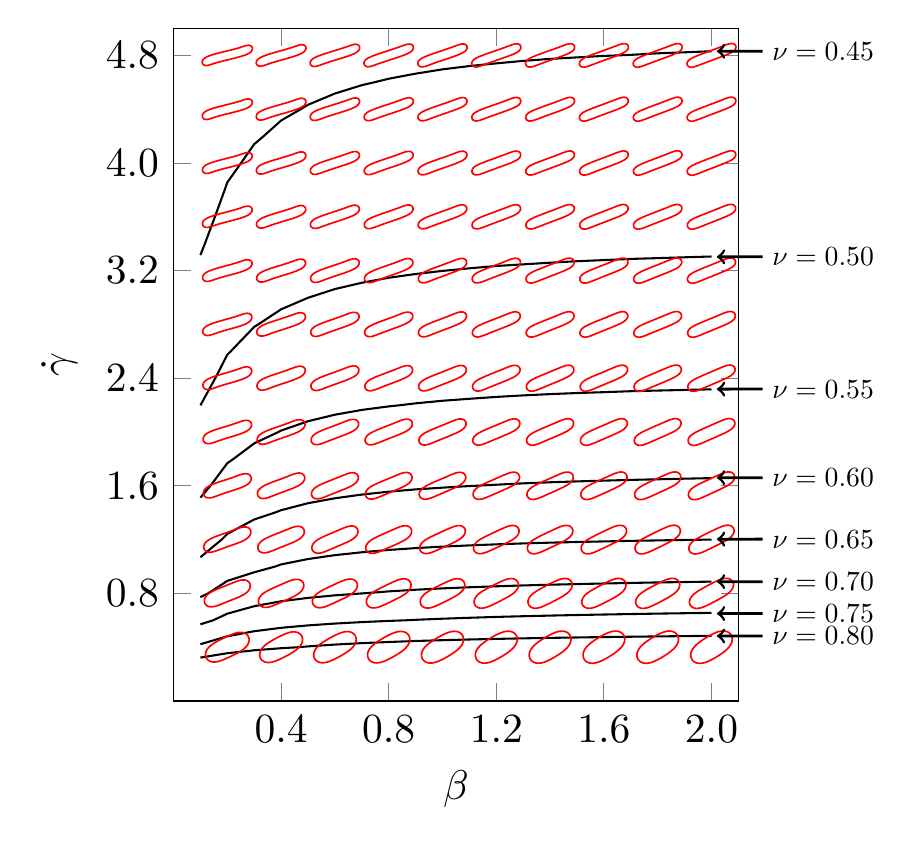
\begin{tikzpicture}[scale=1.5]

  \begin{axis}[
    axis equal image,
    xmin = 0,
    xmax = 21,
    ymin = 0,
    ymax = 25,
    xtick = {4,8,12,16,20},
    xticklabels = {$0.4$,$0.8$,$1.2$,$1.6$,$2.0$},
    xlabel = {$\beta$},
    ytick = {4,8,12,16,20,24},
    yticklabels = {$0.8$,$1.6$,$2.4$,$3.2$,$4.0$,$4.8$},
    ylabel = {$\dot{\gamma}$},
  ]


% START OF CONTOUR LINES WITH CONSTANT REDUCED AREA
% Points with Redcued area of 0.45
\addplot[black,line width=0.5pt] coordinates{
(1.0000e+00,1.6577e+01)
(1.1657e+00,1.7000e+01)
(1.5393e+00,1.8000e+01)
(1.9029e+00,1.9000e+01)
(2.0000e+00,1.9279e+01)
(2.5116e+00,2.0000e+01)
(3.0000e+00,2.0700e+01)
(3.3529e+00,2.1000e+01)
(4.0000e+00,2.1579e+01)
(4.7273e+00,2.2000e+01)
(5.0000e+00,2.2164e+01)
(6.0000e+00,2.2582e+01)
(7.0000e+00,2.2893e+01)
(7.4615e+00,2.3000e+01)
(8.0000e+00,2.3132e+01)
(9.0000e+00,2.3321e+01)
(1.0000e+01,2.3481e+01)
(1.1000e+01,2.3604e+01)
(1.2000e+01,2.3704e+01)
(1.3000e+01,2.3796e+01)
(1.4000e+01,2.3870e+01)
(1.5000e+01,2.3926e+01)
(1.6000e+01,2.3981e+01)
(1.6500e+01,2.4000e+01)
(1.7000e+01,2.4020e+01)
(1.8000e+01,2.4077e+01)
(1.9000e+01,2.4115e+01)
(2.0000e+01,2.4154e+01)
};

% Points with Redcued area of 0.50
\addplot[black,line width=0.5pt] coordinates{
(1.0000e+00,1.0991e+01)
(1.0049e+00,1.1000e+01)
(1.5522e+00,1.2000e+01)
(2.0000e+00,1.2874e+01)
(2.1287e+00,1.3000e+01)
(3.0000e+00,1.3907e+01)
(3.1500e+00,1.4000e+01)
(4.0000e+00,1.4560e+01)
(5.0000e+00,1.4989e+01)
(5.0357e+00,1.5000e+01)
(6.0000e+00,1.5314e+01)
(7.0000e+00,1.5547e+01)
(8.0000e+00,1.5733e+01)
(9.0000e+00,1.5874e+01)
(1.0000e+01,1.5989e+01)
(1.0125e+01,1.6000e+01)
(1.1000e+01,1.6085e+01)
(1.2000e+01,1.6171e+01)
(1.3000e+01,1.6232e+01)
(1.4000e+01,1.6293e+01)
(1.5000e+01,1.6349e+01)
(1.6000e+01,1.6390e+01)
(1.7000e+01,1.6434e+01)
(1.8000e+01,1.6463e+01)
(1.9000e+01,1.6494e+01)
(2.0000e+01,1.6524e+01)
};

% Points with Redcued area of 0.55
\addplot[black,line width=0.5pt] coordinates{
(1.0000e+00,7.5598e+00)
(1.3733e+00,8.0000e+00)
(2.0000e+00,8.8395e+00)
(2.2321e+00,9.0000e+00)
(3.0000e+00,9.5772e+00)
(3.9000e+00,1.0000e+01)
(4.0000e+00,1.0053e+01)
(5.0000e+00,1.0400e+01)
(6.0000e+00,1.0642e+01)
(7.0000e+00,1.0820e+01)
(8.0000e+00,1.0951e+01)
(8.4667e+00,1.1000e+01)
(9.0000e+00,1.1065e+01)
(1.0000e+01,1.1161e+01)
(1.1000e+01,1.1234e+01)
(1.2000e+01,1.1304e+01)
(1.3000e+01,1.1360e+01)
(1.4000e+01,1.1408e+01)
(1.5000e+01,1.1448e+01)
(1.6000e+01,1.1480e+01)
(1.7000e+01,1.1516e+01)
(1.8000e+01,1.1540e+01)
(1.9000e+01,1.1563e+01)
(2.0000e+01,1.1587e+01)
};

% Points with Redcued area of 0.60
\addplot[black,line width=0.5pt] coordinates{
(1.0000e+00,5.3444e+00)
(1.7902e+00,6.0000e+00)
(2.0000e+00,6.2108e+00)
(3.0000e+00,6.7478e+00)
(3.7600e+00,7.0000e+00)
(4.0000e+00,7.0928e+00)
(5.0000e+00,7.3520e+00)
(6.0000e+00,7.5354e+00)
(7.0000e+00,7.6734e+00)
(8.0000e+00,7.7800e+00)
(9.0000e+00,7.8657e+00)
(1.0000e+01,7.9307e+00)
(1.1000e+01,7.9901e+00)
(1.1222e+01,8.0000e+00)
(1.2000e+01,8.0398e+00)
(1.3000e+01,8.0904e+00)
(1.4000e+01,8.1299e+00)
(1.5000e+01,8.1629e+00)
(1.6000e+01,8.1910e+00)
(1.7000e+01,8.2191e+00)
(1.8000e+01,8.2416e+00)
(1.9000e+01,8.2640e+00)
(2.0000e+01,8.2849e+00)
};

% Points with Redcued area of 0.65
\addplot[black,line width=0.5pt] coordinates{
(1.0000e+00,3.8618e+00)
(1.2870e+00,4.0000e+00)
(2.0000e+00,4.4649e+00)
(3.0000e+00,4.7845e+00)
(3.7879e+00,5.0000e+00)
(4.0000e+00,5.0764e+00)
(5.0000e+00,5.2770e+00)
(6.0000e+00,5.4214e+00)
(7.0000e+00,5.5284e+00)
(8.0000e+00,5.6148e+00)
(9.0000e+00,5.6831e+00)
(1.0000e+01,5.7378e+00)
(1.1000e+01,5.7840e+00)
(1.2000e+01,5.8229e+00)
(1.3000e+01,5.8576e+00)
(1.4000e+01,5.8858e+00)
(1.5000e+01,5.9103e+00)
(1.6000e+01,5.9313e+00)
(1.7000e+01,5.9521e+00)
(1.8000e+01,5.9693e+00)
(1.9000e+01,5.9863e+00)
(2.0000e+01,6.0000e+00)
(2.0000e+01,6.0000e+00)
};

% Points with Redcued area of 0.70
\addplot[black,line width=0.5pt] coordinates{
(1.0000e+00,2.8504e+00)
(1.4764e+00,3.0000e+00)
(2.0000e+00,3.2456e+00)
(3.0000e+00,3.5232e+00)
(4.0000e+00,3.7064e+00)
(5.0000e+00,3.8326e+00)
(6.0000e+00,3.9275e+00)
(7.0000e+00,3.9978e+00)
(7.0370e+00,4.0000e+00)
(8.0000e+00,4.0739e+00)
(9.0000e+00,4.1356e+00)
(1.0000e+01,4.1859e+00)
(1.1000e+01,4.2275e+00)
(1.2000e+01,4.2633e+00)
(1.3000e+01,4.2953e+00)
(1.4000e+01,4.3222e+00)
(1.5000e+01,4.3463e+00)
(1.6000e+01,4.3674e+00)
(1.7000e+01,4.3884e+00)
(1.8000e+01,4.4066e+00)
(1.9000e+01,4.4219e+00)
(2.0000e+01,4.4372e+00)
};

% Points with Redcued area of 0.75
\addplot[black,line width=0.5pt] coordinates{
(1.0000e+00,2.1096e+00)
(2.0000e+00,2.4052e+00)
(3.0000e+00,2.5929e+00)
(4.0000e+00,2.7196e+00)
(5.0000e+00,2.8097e+00)
(6.0000e+00,2.8781e+00)
(7.0000e+00,2.9327e+00)
(8.0000e+00,2.9765e+00)
(8.6522e+00,3.0000e+00)
(9.0000e+00,3.0174e+00)
(1.0000e+01,3.0586e+00)
(1.1000e+01,3.0931e+00)
(1.2000e+01,3.1250e+00)
(1.3000e+01,3.1509e+00)
(1.4000e+01,3.1742e+00)
(1.5000e+01,3.1953e+00)
(1.6000e+01,3.2141e+00)
(1.7000e+01,3.2313e+00)
(1.8000e+01,3.2479e+00)
(1.9000e+01,3.2623e+00)
(2.0000e+01,3.2751e+00)
};

% Points with Redcued area of 0.80
\addplot[black,line width=0.5pt] coordinates{
(1.0000e+00,1.6134e+00)
(2.0000e+00,1.7753e+00)
(3.0000e+00,1.8847e+00)
(4.0000e+00,1.9618e+00)
(4.6667e+00,2.0000e+00)
(5.0000e+00,2.0296e+00)
(6.0000e+00,2.0969e+00)
(7.0000e+00,2.1502e+00)
(8.0000e+00,2.1928e+00)
(9.0000e+00,2.2300e+00)
(1.0000e+01,2.2598e+00)
(1.1000e+01,2.2859e+00)
(1.2000e+01,2.3083e+00)
(1.3000e+01,2.3281e+00)
(1.4000e+01,2.3463e+00)
(1.5000e+01,2.3609e+00)
(1.6000e+01,2.3760e+00)
(1.7000e+01,2.3885e+00)
(1.8000e+01,2.4000e+00)
(1.9000e+01,2.4119e+00)
(2.0000e+01,2.4212e+00)
};
% END OF CONTOUR LINES WITH CONSTANT REDUCED AREA



% beta = 0.2,shear rate = 0.4
\addplot[red] coordinates{
(1.8897e+00,2.3503e+00)
(1.8758e+00,2.3437e+00)
(1.8617e+00,2.3369e+00)
(1.8471e+00,2.3299e+00)
(1.8317e+00,2.3225e+00)
(1.8154e+00,2.3146e+00)
(1.7981e+00,2.3061e+00)
(1.7796e+00,2.2971e+00)
(1.7599e+00,2.2873e+00)
(1.7389e+00,2.2768e+00)
(1.7167e+00,2.2656e+00)
(1.6931e+00,2.2535e+00)
(1.6683e+00,2.2406e+00)
(1.6422e+00,2.2268e+00)
(1.6149e+00,2.2120e+00)
(1.5865e+00,2.1963e+00)
(1.5572e+00,2.1794e+00)
(1.5269e+00,2.1614e+00)
(1.4959e+00,2.1421e+00)
(1.4643e+00,2.1214e+00)
(1.4324e+00,2.0991e+00)
(1.4003e+00,2.0751e+00)
(1.3685e+00,2.0491e+00)
(1.3373e+00,2.0210e+00)
(1.3072e+00,1.9905e+00)
(1.2788e+00,1.9574e+00)
(1.2527e+00,1.9216e+00)
(1.2299e+00,1.8830e+00)
(1.2111e+00,1.8416e+00)
(1.1975e+00,1.7980e+00)
(1.1901e+00,1.7525e+00)
(1.1896e+00,1.7063e+00)
(1.1968e+00,1.6606e+00)
(1.2117e+00,1.6168e+00)
(1.2340e+00,1.5765e+00)
(1.2629e+00,1.5409e+00)
(1.2972e+00,1.5109e+00)
(1.3355e+00,1.4870e+00)
(1.3765e+00,1.4693e+00)
(1.4190e+00,1.4574e+00)
(1.4619e+00,1.4507e+00)
(1.5045e+00,1.4484e+00)
(1.5462e+00,1.4499e+00)
(1.5869e+00,1.4544e+00)
(1.6261e+00,1.4613e+00)
(1.6639e+00,1.4699e+00)
(1.7002e+00,1.4798e+00)
(1.7349e+00,1.4905e+00)
(1.7681e+00,1.5018e+00)
(1.7997e+00,1.5134e+00)
(1.8299e+00,1.5251e+00)
(1.8585e+00,1.5366e+00)
(1.8857e+00,1.5479e+00)
(1.9113e+00,1.5589e+00)
(1.9355e+00,1.5694e+00)
(1.9583e+00,1.5795e+00)
(1.9796e+00,1.5891e+00)
(1.9996e+00,1.5981e+00)
(2.0183e+00,1.6067e+00)
(2.0357e+00,1.6148e+00)
(2.0521e+00,1.6224e+00)
(2.0676e+00,1.6296e+00)
(2.0823e+00,1.6365e+00)
(2.0964e+00,1.6432e+00)
(2.1103e+00,1.6497e+00)
(2.1242e+00,1.6563e+00)
(2.1383e+00,1.6631e+00)
(2.1529e+00,1.6701e+00)
(2.1683e+00,1.6775e+00)
(2.1846e+00,1.6854e+00)
(2.2019e+00,1.6939e+00)
(2.2204e+00,1.7029e+00)
(2.2401e+00,1.7127e+00)
(2.2611e+00,1.7232e+00)
(2.2833e+00,1.7344e+00)
(2.3069e+00,1.7465e+00)
(2.3317e+00,1.7594e+00)
(2.3578e+00,1.7732e+00)
(2.3851e+00,1.7880e+00)
(2.4135e+00,1.8037e+00)
(2.4428e+00,1.8206e+00)
(2.4731e+00,1.8386e+00)
(2.5041e+00,1.8579e+00)
(2.5357e+00,1.8786e+00)
(2.5676e+00,1.9009e+00)
(2.5997e+00,1.9249e+00)
(2.6315e+00,1.9509e+00)
(2.6627e+00,1.9790e+00)
(2.6928e+00,2.0095e+00)
(2.7212e+00,2.0426e+00)
(2.7473e+00,2.0784e+00)
(2.7701e+00,2.1170e+00)
(2.7889e+00,2.1584e+00)
(2.8025e+00,2.2020e+00)
(2.8099e+00,2.2475e+00)
(2.8104e+00,2.2937e+00)
(2.8032e+00,2.3394e+00)
(2.7883e+00,2.3832e+00)
(2.7660e+00,2.4235e+00)
(2.7371e+00,2.4591e+00)
(2.7028e+00,2.4891e+00)
(2.6645e+00,2.5130e+00)
(2.6235e+00,2.5307e+00)
(2.5810e+00,2.5426e+00)
(2.5381e+00,2.5493e+00)
(2.4955e+00,2.5516e+00)
(2.4538e+00,2.5501e+00)
(2.4131e+00,2.5456e+00)
(2.3739e+00,2.5387e+00)
(2.3361e+00,2.5301e+00)
(2.2998e+00,2.5202e+00)
(2.2651e+00,2.5095e+00)
(2.2319e+00,2.4982e+00)
(2.2003e+00,2.4866e+00)
(2.1701e+00,2.4749e+00)
(2.1415e+00,2.4634e+00)
(2.1143e+00,2.4521e+00)
(2.0887e+00,2.4411e+00)
(2.0645e+00,2.4306e+00)
(2.0417e+00,2.4205e+00)
(2.0204e+00,2.4109e+00)
(2.0004e+00,2.4019e+00)
(1.9817e+00,2.3933e+00)
(1.9643e+00,2.3852e+00)
(1.9479e+00,2.3776e+00)
(1.9324e+00,2.3704e+00)
(1.9177e+00,2.3635e+00)
(1.9036e+00,2.3568e+00)
(1.8897e+00,2.3503e+00)
};

% beta = 0.4,shear rate = 0.4
\addplot[red] coordinates{
(4.0227e+00,2.4358e+00)
(4.0088e+00,2.4292e+00)
(3.9947e+00,2.4224e+00)
(3.9801e+00,2.4153e+00)
(3.9648e+00,2.4079e+00)
(3.9486e+00,2.3999e+00)
(3.9313e+00,2.3913e+00)
(3.9129e+00,2.3820e+00)
(3.8933e+00,2.3721e+00)
(3.8725e+00,2.3614e+00)
(3.8503e+00,2.3500e+00)
(3.8269e+00,2.3377e+00)
(3.8021e+00,2.3246e+00)
(3.7761e+00,2.3107e+00)
(3.7489e+00,2.2959e+00)
(3.7205e+00,2.2803e+00)
(3.6910e+00,2.2637e+00)
(3.6604e+00,2.2462e+00)
(3.6289e+00,2.2278e+00)
(3.5966e+00,2.2082e+00)
(3.5636e+00,2.1876e+00)
(3.5300e+00,2.1658e+00)
(3.4961e+00,2.1427e+00)
(3.4621e+00,2.1181e+00)
(3.4281e+00,2.0919e+00)
(3.3947e+00,2.0640e+00)
(3.3620e+00,2.0340e+00)
(3.3306e+00,2.0020e+00)
(3.3010e+00,1.9676e+00)
(3.2739e+00,1.9308e+00)
(3.2499e+00,1.8915e+00)
(3.2299e+00,1.8498e+00)
(3.2148e+00,1.8060e+00)
(3.2054e+00,1.7606e+00)
(3.2026e+00,1.7145e+00)
(3.2067e+00,1.6687e+00)
(3.2181e+00,1.6245e+00)
(3.2365e+00,1.5832e+00)
(3.2612e+00,1.5459e+00)
(3.2913e+00,1.5136e+00)
(3.3254e+00,1.4868e+00)
(3.3625e+00,1.4656e+00)
(3.4012e+00,1.4499e+00)
(3.4406e+00,1.4393e+00)
(3.4800e+00,1.4330e+00)
(3.5187e+00,1.4306e+00)
(3.5562e+00,1.4312e+00)
(3.5924e+00,1.4343e+00)
(3.6271e+00,1.4394e+00)
(3.6602e+00,1.4459e+00)
(3.6916e+00,1.4535e+00)
(3.7213e+00,1.4618e+00)
(3.7494e+00,1.4706e+00)
(3.7758e+00,1.4795e+00)
(3.8006e+00,1.4885e+00)
(3.8239e+00,1.4973e+00)
(3.8456e+00,1.5060e+00)
(3.8659e+00,1.5144e+00)
(3.8848e+00,1.5224e+00)
(3.9025e+00,1.5300e+00)
(3.9190e+00,1.5374e+00)
(3.9345e+00,1.5444e+00)
(3.9492e+00,1.5511e+00)
(3.9634e+00,1.5577e+00)
(3.9773e+00,1.5642e+00)
(3.9912e+00,1.5708e+00)
(4.0053e+00,1.5776e+00)
(4.0199e+00,1.5847e+00)
(4.0352e+00,1.5921e+00)
(4.0514e+00,1.6001e+00)
(4.0687e+00,1.6087e+00)
(4.0871e+00,1.6180e+00)
(4.1067e+00,1.6279e+00)
(4.1275e+00,1.6386e+00)
(4.1497e+00,1.6500e+00)
(4.1731e+00,1.6623e+00)
(4.1979e+00,1.6754e+00)
(4.2239e+00,1.6893e+00)
(4.2511e+00,1.7041e+00)
(4.2795e+00,1.7197e+00)
(4.3090e+00,1.7363e+00)
(4.3396e+00,1.7538e+00)
(4.3711e+00,1.7722e+00)
(4.4034e+00,1.7918e+00)
(4.4364e+00,1.8124e+00)
(4.4700e+00,1.8342e+00)
(4.5039e+00,1.8573e+00)
(4.5379e+00,1.8819e+00)
(4.5719e+00,1.9081e+00)
(4.6053e+00,1.9360e+00)
(4.6380e+00,1.9660e+00)
(4.6694e+00,1.9980e+00)
(4.6990e+00,2.0324e+00)
(4.7261e+00,2.0692e+00)
(4.7501e+00,2.1085e+00)
(4.7701e+00,2.1502e+00)
(4.7852e+00,2.1940e+00)
(4.7946e+00,2.2394e+00)
(4.7974e+00,2.2855e+00)
(4.7933e+00,2.3313e+00)
(4.7819e+00,2.3755e+00)
(4.7635e+00,2.4168e+00)
(4.7388e+00,2.4541e+00)
(4.7087e+00,2.4864e+00)
(4.6746e+00,2.5132e+00)
(4.6375e+00,2.5344e+00)
(4.5988e+00,2.5501e+00)
(4.5594e+00,2.5607e+00)
(4.5200e+00,2.5670e+00)
(4.4813e+00,2.5694e+00)
(4.4438e+00,2.5688e+00)
(4.4076e+00,2.5657e+00)
(4.3729e+00,2.5606e+00)
(4.3398e+00,2.5541e+00)
(4.3084e+00,2.5465e+00)
(4.2787e+00,2.5382e+00)
(4.2506e+00,2.5294e+00)
(4.2242e+00,2.5205e+00)
(4.1994e+00,2.5115e+00)
(4.1761e+00,2.5027e+00)
(4.1544e+00,2.4940e+00)
(4.1341e+00,2.4856e+00)
(4.1152e+00,2.4776e+00)
(4.0975e+00,2.4700e+00)
(4.0810e+00,2.4626e+00)
(4.0655e+00,2.4556e+00)
(4.0508e+00,2.4489e+00)
(4.0366e+00,2.4423e+00)
(4.0227e+00,2.4358e+00)
};

% beta = 0.6,shear rate = 0.4
\addplot[red] coordinates{
(6.0938e+00,2.4822e+00)
(6.0798e+00,2.4759e+00)
(6.0656e+00,2.4694e+00)
(6.0509e+00,2.4625e+00)
(6.0355e+00,2.4553e+00)
(6.0192e+00,2.4474e+00)
(6.0019e+00,2.4390e+00)
(5.9835e+00,2.4298e+00)
(5.9639e+00,2.4200e+00)
(5.9430e+00,2.4093e+00)
(5.9208e+00,2.3979e+00)
(5.8974e+00,2.3856e+00)
(5.8727e+00,2.3724e+00)
(5.8468e+00,2.3584e+00)
(5.8196e+00,2.3435e+00)
(5.7913e+00,2.3278e+00)
(5.7618e+00,2.3111e+00)
(5.7313e+00,2.2936e+00)
(5.6998e+00,2.2751e+00)
(5.6674e+00,2.2557e+00)
(5.6343e+00,2.2353e+00)
(5.6005e+00,2.2139e+00)
(5.5661e+00,2.1914e+00)
(5.5315e+00,2.1677e+00)
(5.4967e+00,2.1427e+00)
(5.4620e+00,2.1163e+00)
(5.4277e+00,2.0883e+00)
(5.3940e+00,2.0587e+00)
(5.3615e+00,2.0271e+00)
(5.3304e+00,1.9935e+00)
(5.3015e+00,1.9577e+00)
(5.2752e+00,1.9196e+00)
(5.2523e+00,1.8793e+00)
(5.2337e+00,1.8369e+00)
(5.2200e+00,1.7928e+00)
(5.2121e+00,1.7474e+00)
(5.2105e+00,1.7018e+00)
(5.2157e+00,1.6568e+00)
(5.2277e+00,1.6136e+00)
(5.2461e+00,1.5735e+00)
(5.2703e+00,1.5374e+00)
(5.2993e+00,1.5061e+00)
(5.3319e+00,1.4799e+00)
(5.3670e+00,1.4590e+00)
(5.4036e+00,1.4432e+00)
(5.4407e+00,1.4320e+00)
(5.4776e+00,1.4249e+00)
(5.5138e+00,1.4213e+00)
(5.5488e+00,1.4206e+00)
(5.5825e+00,1.4222e+00)
(5.6146e+00,1.4257e+00)
(5.6451e+00,1.4305e+00)
(5.6739e+00,1.4364e+00)
(5.7010e+00,1.4430e+00)
(5.7264e+00,1.4500e+00)
(5.7502e+00,1.4572e+00)
(5.7724e+00,1.4645e+00)
(5.7931e+00,1.4718e+00)
(5.8124e+00,1.4789e+00)
(5.8304e+00,1.4859e+00)
(5.8471e+00,1.4926e+00)
(5.8629e+00,1.4990e+00)
(5.8778e+00,1.5054e+00)
(5.8922e+00,1.5116e+00)
(5.9062e+00,1.5178e+00)
(5.9202e+00,1.5241e+00)
(5.9344e+00,1.5306e+00)
(5.9491e+00,1.5375e+00)
(5.9645e+00,1.5447e+00)
(5.9808e+00,1.5526e+00)
(5.9981e+00,1.5610e+00)
(6.0165e+00,1.5702e+00)
(6.0361e+00,1.5800e+00)
(6.0570e+00,1.5907e+00)
(6.0792e+00,1.6021e+00)
(6.1026e+00,1.6144e+00)
(6.1273e+00,1.6276e+00)
(6.1532e+00,1.6416e+00)
(6.1804e+00,1.6565e+00)
(6.2087e+00,1.6722e+00)
(6.2382e+00,1.6889e+00)
(6.2687e+00,1.7064e+00)
(6.3002e+00,1.7249e+00)
(6.3326e+00,1.7443e+00)
(6.3657e+00,1.7647e+00)
(6.3995e+00,1.7861e+00)
(6.4339e+00,1.8086e+00)
(6.4685e+00,1.8323e+00)
(6.5033e+00,1.8573e+00)
(6.5380e+00,1.8837e+00)
(6.5723e+00,1.9117e+00)
(6.6060e+00,1.9413e+00)
(6.6385e+00,1.9729e+00)
(6.6696e+00,2.0065e+00)
(6.6985e+00,2.0423e+00)
(6.7248e+00,2.0804e+00)
(6.7477e+00,2.1207e+00)
(6.7663e+00,2.1631e+00)
(6.7800e+00,2.2072e+00)
(6.7879e+00,2.2526e+00)
(6.7895e+00,2.2982e+00)
(6.7843e+00,2.3432e+00)
(6.7723e+00,2.3864e+00)
(6.7539e+00,2.4265e+00)
(6.7297e+00,2.4626e+00)
(6.7007e+00,2.4939e+00)
(6.6681e+00,2.5201e+00)
(6.6330e+00,2.5410e+00)
(6.5964e+00,2.5568e+00)
(6.5593e+00,2.5680e+00)
(6.5224e+00,2.5751e+00)
(6.4862e+00,2.5787e+00)
(6.4512e+00,2.5794e+00)
(6.4175e+00,2.5778e+00)
(6.3854e+00,2.5743e+00)
(6.3549e+00,2.5695e+00)
(6.3261e+00,2.5636e+00)
(6.2990e+00,2.5570e+00)
(6.2736e+00,2.5500e+00)
(6.2498e+00,2.5428e+00)
(6.2276e+00,2.5355e+00)
(6.2069e+00,2.5282e+00)
(6.1876e+00,2.5211e+00)
(6.1696e+00,2.5141e+00)
(6.1529e+00,2.5074e+00)
(6.1371e+00,2.5010e+00)
(6.1222e+00,2.4946e+00)
(6.1078e+00,2.4884e+00)
(6.0938e+00,2.4822e+00)
};

% beta = 0.8,shear rate = 0.4
\addplot[red] coordinates{
(8.1391e+00,2.5110e+00)
(8.1249e+00,2.5050e+00)
(8.1106e+00,2.4988e+00)
(8.0957e+00,2.4923e+00)
(8.0802e+00,2.4853e+00)
(8.0638e+00,2.4777e+00)
(8.0464e+00,2.4695e+00)
(8.0279e+00,2.4605e+00)
(8.0082e+00,2.4508e+00)
(7.9872e+00,2.4403e+00)
(7.9651e+00,2.4290e+00)
(7.9416e+00,2.4167e+00)
(7.9169e+00,2.4036e+00)
(7.8910e+00,2.3896e+00)
(7.8638e+00,2.3747e+00)
(7.8355e+00,2.3589e+00)
(7.8061e+00,2.3421e+00)
(7.7757e+00,2.3245e+00)
(7.7442e+00,2.3059e+00)
(7.7119e+00,2.2865e+00)
(7.6788e+00,2.2661e+00)
(7.6450e+00,2.2447e+00)
(7.6106e+00,2.2223e+00)
(7.5757e+00,2.1989e+00)
(7.5407e+00,2.1743e+00)
(7.5055e+00,2.1485e+00)
(7.4705e+00,2.1214e+00)
(7.4359e+00,2.0928e+00)
(7.4021e+00,2.0626e+00)
(7.3694e+00,2.0306e+00)
(7.3382e+00,1.9968e+00)
(7.3090e+00,1.9609e+00)
(7.2826e+00,1.9228e+00)
(7.2594e+00,1.8827e+00)
(7.2403e+00,1.8406e+00)
(7.2261e+00,1.7968e+00)
(7.2174e+00,1.7520e+00)
(7.2148e+00,1.7067e+00)
(7.2187e+00,1.6621e+00)
(7.2292e+00,1.6192e+00)
(7.2459e+00,1.5790e+00)
(7.2682e+00,1.5426e+00)
(7.2952e+00,1.5106e+00)
(7.3258e+00,1.4835e+00)
(7.3590e+00,1.4615e+00)
(7.3937e+00,1.4442e+00)
(7.4291e+00,1.4314e+00)
(7.4643e+00,1.4227e+00)
(7.4990e+00,1.4173e+00)
(7.5326e+00,1.4149e+00)
(7.5649e+00,1.4148e+00)
(7.5957e+00,1.4167e+00)
(7.6249e+00,1.4199e+00)
(7.6525e+00,1.4243e+00)
(7.6784e+00,1.4295e+00)
(7.7026e+00,1.4352e+00)
(7.7252e+00,1.4412e+00)
(7.7463e+00,1.4473e+00)
(7.7658e+00,1.4535e+00)
(7.7841e+00,1.4596e+00)
(7.8011e+00,1.4657e+00)
(7.8170e+00,1.4716e+00)
(7.8322e+00,1.4774e+00)
(7.8467e+00,1.4832e+00)
(7.8609e+00,1.4890e+00)
(7.8751e+00,1.4950e+00)
(7.8894e+00,1.5012e+00)
(7.9043e+00,1.5077e+00)
(7.9198e+00,1.5147e+00)
(7.9362e+00,1.5223e+00)
(7.9536e+00,1.5305e+00)
(7.9721e+00,1.5395e+00)
(7.9918e+00,1.5492e+00)
(8.0128e+00,1.5597e+00)
(8.0349e+00,1.5710e+00)
(8.0584e+00,1.5833e+00)
(8.0831e+00,1.5964e+00)
(8.1090e+00,1.6104e+00)
(8.1362e+00,1.6253e+00)
(8.1645e+00,1.6411e+00)
(8.1939e+00,1.6579e+00)
(8.2243e+00,1.6755e+00)
(8.2558e+00,1.6941e+00)
(8.2881e+00,1.7135e+00)
(8.3212e+00,1.7339e+00)
(8.3550e+00,1.7553e+00)
(8.3894e+00,1.7777e+00)
(8.4243e+00,1.8011e+00)
(8.4593e+00,1.8257e+00)
(8.4945e+00,1.8515e+00)
(8.5295e+00,1.8786e+00)
(8.5641e+00,1.9072e+00)
(8.5979e+00,1.9374e+00)
(8.6306e+00,1.9694e+00)
(8.6618e+00,2.0032e+00)
(8.6910e+00,2.0391e+00)
(8.7174e+00,2.0772e+00)
(8.7406e+00,2.1173e+00)
(8.7597e+00,2.1594e+00)
(8.7739e+00,2.2032e+00)
(8.7826e+00,2.2480e+00)
(8.7852e+00,2.2933e+00)
(8.7813e+00,2.3379e+00)
(8.7708e+00,2.3808e+00)
(8.7541e+00,2.4210e+00)
(8.7318e+00,2.4574e+00)
(8.7048e+00,2.4894e+00)
(8.6742e+00,2.5165e+00)
(8.6410e+00,2.5385e+00)
(8.6063e+00,2.5558e+00)
(8.5709e+00,2.5686e+00)
(8.5357e+00,2.5773e+00)
(8.5010e+00,2.5827e+00)
(8.4674e+00,2.5851e+00)
(8.4351e+00,2.5852e+00)
(8.4043e+00,2.5833e+00)
(8.3751e+00,2.5801e+00)
(8.3475e+00,2.5757e+00)
(8.3216e+00,2.5705e+00)
(8.2974e+00,2.5648e+00)
(8.2748e+00,2.5588e+00)
(8.2537e+00,2.5527e+00)
(8.2342e+00,2.5465e+00)
(8.2159e+00,2.5404e+00)
(8.1989e+00,2.5343e+00)
(8.1830e+00,2.5284e+00)
(8.1678e+00,2.5226e+00)
(8.1533e+00,2.5168e+00)
(8.1391e+00,2.5110e+00)
};

% beta = 1,shear rate = 0.4
\addplot[red] coordinates{
(1.0171e+01,2.5303e+00)
(1.0157e+01,2.5247e+00)
(1.0143e+01,2.5188e+00)
(1.0128e+01,2.5125e+00)
(1.0112e+01,2.5058e+00)
(1.0095e+01,2.4985e+00)
(1.0078e+01,2.4905e+00)
(1.0059e+01,2.4818e+00)
(1.0040e+01,2.4723e+00)
(1.0019e+01,2.4620e+00)
(9.9962e+00,2.4508e+00)
(9.9727e+00,2.4387e+00)
(9.9480e+00,2.4257e+00)
(9.9220e+00,2.4118e+00)
(9.8948e+00,2.3969e+00)
(9.8665e+00,2.3811e+00)
(9.8371e+00,2.3644e+00)
(9.8067e+00,2.3467e+00)
(9.7752e+00,2.3282e+00)
(9.7429e+00,2.3087e+00)
(9.7098e+00,2.2883e+00)
(9.6760e+00,2.2669e+00)
(9.6416e+00,2.2446e+00)
(9.6067e+00,2.2212e+00)
(9.5715e+00,2.1969e+00)
(9.5361e+00,2.1714e+00)
(9.5008e+00,2.1446e+00)
(9.4658e+00,2.1166e+00)
(9.4313e+00,2.0871e+00)
(9.3977e+00,2.0561e+00)
(9.3654e+00,2.0233e+00)
(9.3348e+00,1.9887e+00)
(9.3064e+00,1.9521e+00)
(9.2808e+00,1.9134e+00)
(9.2586e+00,1.8729e+00)
(9.2407e+00,1.8305e+00)
(9.2276e+00,1.7867e+00)
(9.2201e+00,1.7420e+00)
(9.2187e+00,1.6972e+00)
(9.2235e+00,1.6532e+00)
(9.2346e+00,1.6112e+00)
(9.2517e+00,1.5720e+00)
(9.2740e+00,1.5366e+00)
(9.3006e+00,1.5055e+00)
(9.3306e+00,1.4792e+00)
(9.3628e+00,1.4577e+00)
(9.3964e+00,1.4408e+00)
(9.4305e+00,1.4281e+00)
(9.4644e+00,1.4192e+00)
(9.4976e+00,1.4136e+00)
(9.5298e+00,1.4108e+00)
(9.5607e+00,1.4101e+00)
(9.5900e+00,1.4113e+00)
(9.6178e+00,1.4139e+00)
(9.6440e+00,1.4175e+00)
(9.6685e+00,1.4218e+00)
(9.6913e+00,1.4267e+00)
(9.7126e+00,1.4319e+00)
(9.7325e+00,1.4373e+00)
(9.7509e+00,1.4427e+00)
(9.7681e+00,1.4481e+00)
(9.7843e+00,1.4535e+00)
(9.7996e+00,1.4589e+00)
(9.8143e+00,1.4643e+00)
(9.8286e+00,1.4697e+00)
(9.8429e+00,1.4753e+00)
(9.8574e+00,1.4812e+00)
(9.8723e+00,1.4875e+00)
(9.8880e+00,1.4942e+00)
(9.9045e+00,1.5015e+00)
(9.9220e+00,1.5095e+00)
(9.9407e+00,1.5182e+00)
(9.9605e+00,1.5277e+00)
(9.9815e+00,1.5380e+00)
(1.0004e+01,1.5492e+00)
(1.0027e+01,1.5613e+00)
(1.0052e+01,1.5743e+00)
(1.0078e+01,1.5882e+00)
(1.0105e+01,1.6031e+00)
(1.0133e+01,1.6189e+00)
(1.0163e+01,1.6356e+00)
(1.0193e+01,1.6533e+00)
(1.0225e+01,1.6718e+00)
(1.0257e+01,1.6913e+00)
(1.0290e+01,1.7117e+00)
(1.0324e+01,1.7331e+00)
(1.0358e+01,1.7554e+00)
(1.0393e+01,1.7788e+00)
(1.0429e+01,1.8031e+00)
(1.0464e+01,1.8286e+00)
(1.0499e+01,1.8554e+00)
(1.0534e+01,1.8834e+00)
(1.0569e+01,1.9129e+00)
(1.0602e+01,1.9439e+00)
(1.0635e+01,1.9767e+00)
(1.0665e+01,2.0113e+00)
(1.0694e+01,2.0479e+00)
(1.0719e+01,2.0866e+00)
(1.0741e+01,2.1271e+00)
(1.0759e+01,2.1695e+00)
(1.0772e+01,2.2133e+00)
(1.0780e+01,2.2580e+00)
(1.0781e+01,2.3028e+00)
(1.0776e+01,2.3468e+00)
(1.0765e+01,2.3888e+00)
(1.0748e+01,2.4280e+00)
(1.0726e+01,2.4634e+00)
(1.0699e+01,2.4945e+00)
(1.0669e+01,2.5208e+00)
(1.0637e+01,2.5423e+00)
(1.0604e+01,2.5592e+00)
(1.0570e+01,2.5719e+00)
(1.0536e+01,2.5808e+00)
(1.0502e+01,2.5864e+00)
(1.0470e+01,2.5892e+00)
(1.0439e+01,2.5899e+00)
(1.0410e+01,2.5887e+00)
(1.0382e+01,2.5861e+00)
(1.0356e+01,2.5825e+00)
(1.0332e+01,2.5782e+00)
(1.0309e+01,2.5733e+00)
(1.0287e+01,2.5681e+00)
(1.0268e+01,2.5627e+00)
(1.0249e+01,2.5573e+00)
(1.0232e+01,2.5519e+00)
(1.0216e+01,2.5465e+00)
(1.0200e+01,2.5411e+00)
(1.0186e+01,2.5357e+00)
(1.0171e+01,2.5303e+00)
};

% beta = 1.2,shear rate = 0.4
\addplot[red] coordinates{
(1.2196e+01,2.5437e+00)
(1.2181e+01,2.5384e+00)
(1.2167e+01,2.5328e+00)
(1.2152e+01,2.5268e+00)
(1.2136e+01,2.5203e+00)
(1.2119e+01,2.5133e+00)
(1.2102e+01,2.5055e+00)
(1.2083e+01,2.4971e+00)
(1.2063e+01,2.4878e+00)
(1.2042e+01,2.4777e+00)
(1.2020e+01,2.4667e+00)
(1.1996e+01,2.4547e+00)
(1.1971e+01,2.4419e+00)
(1.1945e+01,2.4281e+00)
(1.1918e+01,2.4133e+00)
(1.1890e+01,2.3976e+00)
(1.1860e+01,2.3810e+00)
(1.1830e+01,2.3634e+00)
(1.1798e+01,2.3448e+00)
(1.1766e+01,2.3254e+00)
(1.1733e+01,2.3050e+00)
(1.1699e+01,2.2837e+00)
(1.1664e+01,2.2615e+00)
(1.1629e+01,2.2383e+00)
(1.1594e+01,2.2140e+00)
(1.1559e+01,2.1887e+00)
(1.1523e+01,2.1623e+00)
(1.1488e+01,2.1346e+00)
(1.1453e+01,2.1056e+00)
(1.1419e+01,2.0751e+00)
(1.1386e+01,2.0430e+00)
(1.1354e+01,2.0091e+00)
(1.1325e+01,1.9734e+00)
(1.1298e+01,1.9358e+00)
(1.1274e+01,1.8962e+00)
(1.1254e+01,1.8549e+00)
(1.1238e+01,1.8120e+00)
(1.1227e+01,1.7679e+00)
(1.1222e+01,1.7234e+00)
(1.1223e+01,1.6792e+00)
(1.1230e+01,1.6362e+00)
(1.1243e+01,1.5955e+00)
(1.1261e+01,1.5579e+00)
(1.1284e+01,1.5242e+00)
(1.1311e+01,1.4949e+00)
(1.1341e+01,1.4702e+00)
(1.1373e+01,1.4502e+00)
(1.1406e+01,1.4346e+00)
(1.1439e+01,1.4229e+00)
(1.1472e+01,1.4148e+00)
(1.1504e+01,1.4097e+00)
(1.1534e+01,1.4071e+00)
(1.1564e+01,1.4066e+00)
(1.1592e+01,1.4077e+00)
(1.1618e+01,1.4100e+00)
(1.1643e+01,1.4133e+00)
(1.1666e+01,1.4173e+00)
(1.1687e+01,1.4217e+00)
(1.1707e+01,1.4264e+00)
(1.1726e+01,1.4312e+00)
(1.1743e+01,1.4362e+00)
(1.1759e+01,1.4411e+00)
(1.1775e+01,1.4461e+00)
(1.1790e+01,1.4511e+00)
(1.1804e+01,1.4563e+00)
(1.1819e+01,1.4616e+00)
(1.1833e+01,1.4672e+00)
(1.1848e+01,1.4732e+00)
(1.1864e+01,1.4797e+00)
(1.1881e+01,1.4867e+00)
(1.1898e+01,1.4945e+00)
(1.1917e+01,1.5029e+00)
(1.1937e+01,1.5122e+00)
(1.1958e+01,1.5223e+00)
(1.1980e+01,1.5333e+00)
(1.2004e+01,1.5453e+00)
(1.2029e+01,1.5581e+00)
(1.2055e+01,1.5719e+00)
(1.2082e+01,1.5867e+00)
(1.2110e+01,1.6024e+00)
(1.2140e+01,1.6190e+00)
(1.2170e+01,1.6366e+00)
(1.2202e+01,1.6552e+00)
(1.2234e+01,1.6746e+00)
(1.2267e+01,1.6950e+00)
(1.2301e+01,1.7163e+00)
(1.2336e+01,1.7385e+00)
(1.2371e+01,1.7617e+00)
(1.2406e+01,1.7860e+00)
(1.2441e+01,1.8113e+00)
(1.2477e+01,1.8377e+00)
(1.2512e+01,1.8654e+00)
(1.2547e+01,1.8944e+00)
(1.2581e+01,1.9249e+00)
(1.2614e+01,1.9570e+00)
(1.2646e+01,1.9909e+00)
(1.2675e+01,2.0266e+00)
(1.2702e+01,2.0642e+00)
(1.2726e+01,2.1038e+00)
(1.2746e+01,2.1451e+00)
(1.2762e+01,2.1880e+00)
(1.2773e+01,2.2321e+00)
(1.2778e+01,2.2766e+00)
(1.2777e+01,2.3208e+00)
(1.2770e+01,2.3638e+00)
(1.2757e+01,2.4045e+00)
(1.2739e+01,2.4421e+00)
(1.2716e+01,2.4758e+00)
(1.2689e+01,2.5051e+00)
(1.2659e+01,2.5298e+00)
(1.2627e+01,2.5498e+00)
(1.2594e+01,2.5654e+00)
(1.2561e+01,2.5771e+00)
(1.2528e+01,2.5852e+00)
(1.2496e+01,2.5903e+00)
(1.2466e+01,2.5929e+00)
(1.2436e+01,2.5934e+00)
(1.2408e+01,2.5923e+00)
(1.2382e+01,2.5900e+00)
(1.2357e+01,2.5867e+00)
(1.2334e+01,2.5827e+00)
(1.2313e+01,2.5783e+00)
(1.2293e+01,2.5736e+00)
(1.2274e+01,2.5688e+00)
(1.2257e+01,2.5638e+00)
(1.2241e+01,2.5589e+00)
(1.2225e+01,2.5539e+00)
(1.2210e+01,2.5489e+00)
(1.2196e+01,2.5437e+00)
};

% beta = 1.4,shear rate = 0.4
\addplot[red] coordinates{
(1.4215e+01,2.5543e+00)
(1.4201e+01,2.5492e+00)
(1.4186e+01,2.5439e+00)
(1.4171e+01,2.5381e+00)
(1.4155e+01,2.5319e+00)
(1.4138e+01,2.5250e+00)
(1.4120e+01,2.5175e+00)
(1.4102e+01,2.5092e+00)
(1.4082e+01,2.5002e+00)
(1.4060e+01,2.4902e+00)
(1.4038e+01,2.4794e+00)
(1.4014e+01,2.4676e+00)
(1.3989e+01,2.4549e+00)
(1.3963e+01,2.4412e+00)
(1.3936e+01,2.4265e+00)
(1.3908e+01,2.4108e+00)
(1.3878e+01,2.3942e+00)
(1.3848e+01,2.3767e+00)
(1.3816e+01,2.3582e+00)
(1.3784e+01,2.3387e+00)
(1.3751e+01,2.3184e+00)
(1.3717e+01,2.2971e+00)
(1.3682e+01,2.2748e+00)
(1.3647e+01,2.2516e+00)
(1.3612e+01,2.2275e+00)
(1.3576e+01,2.2022e+00)
(1.3541e+01,2.1759e+00)
(1.3505e+01,2.1484e+00)
(1.3470e+01,2.1197e+00)
(1.3436e+01,2.0895e+00)
(1.3403e+01,2.0579e+00)
(1.3370e+01,2.0246e+00)
(1.3340e+01,1.9896e+00)
(1.3312e+01,1.9527e+00)
(1.3287e+01,1.9140e+00)
(1.3265e+01,1.8735e+00)
(1.3247e+01,1.8314e+00)
(1.3234e+01,1.7880e+00)
(1.3226e+01,1.7439e+00)
(1.3224e+01,1.6997e+00)
(1.3228e+01,1.6563e+00)
(1.3238e+01,1.6147e+00)
(1.3253e+01,1.5758e+00)
(1.3273e+01,1.5403e+00)
(1.3298e+01,1.5089e+00)
(1.3326e+01,1.4819e+00)
(1.3356e+01,1.4595e+00)
(1.3388e+01,1.4415e+00)
(1.3420e+01,1.4276e+00)
(1.3452e+01,1.4174e+00)
(1.3484e+01,1.4104e+00)
(1.3514e+01,1.4061e+00)
(1.3543e+01,1.4040e+00)
(1.3571e+01,1.4038e+00)
(1.3598e+01,1.4050e+00)
(1.3622e+01,1.4073e+00)
(1.3646e+01,1.4104e+00)
(1.3667e+01,1.4141e+00)
(1.3687e+01,1.4182e+00)
(1.3706e+01,1.4225e+00)
(1.3724e+01,1.4270e+00)
(1.3740e+01,1.4315e+00)
(1.3756e+01,1.4362e+00)
(1.3770e+01,1.4409e+00)
(1.3785e+01,1.4457e+00)
(1.3799e+01,1.4508e+00)
(1.3814e+01,1.4561e+00)
(1.3829e+01,1.4619e+00)
(1.3845e+01,1.4681e+00)
(1.3862e+01,1.4750e+00)
(1.3880e+01,1.4825e+00)
(1.3898e+01,1.4908e+00)
(1.3918e+01,1.4998e+00)
(1.3940e+01,1.5098e+00)
(1.3962e+01,1.5206e+00)
(1.3986e+01,1.5324e+00)
(1.4011e+01,1.5451e+00)
(1.4037e+01,1.5588e+00)
(1.4064e+01,1.5735e+00)
(1.4092e+01,1.5892e+00)
(1.4122e+01,1.6058e+00)
(1.4152e+01,1.6233e+00)
(1.4184e+01,1.6418e+00)
(1.4216e+01,1.6613e+00)
(1.4249e+01,1.6816e+00)
(1.4283e+01,1.7029e+00)
(1.4318e+01,1.7252e+00)
(1.4353e+01,1.7484e+00)
(1.4388e+01,1.7725e+00)
(1.4424e+01,1.7978e+00)
(1.4459e+01,1.8241e+00)
(1.4495e+01,1.8516e+00)
(1.4530e+01,1.8803e+00)
(1.4564e+01,1.9105e+00)
(1.4597e+01,1.9421e+00)
(1.4630e+01,1.9754e+00)
(1.4660e+01,2.0104e+00)
(1.4688e+01,2.0473e+00)
(1.4713e+01,2.0860e+00)
(1.4735e+01,2.1265e+00)
(1.4753e+01,2.1686e+00)
(1.4766e+01,2.2120e+00)
(1.4774e+01,2.2561e+00)
(1.4776e+01,2.3003e+00)
(1.4772e+01,2.3437e+00)
(1.4762e+01,2.3853e+00)
(1.4747e+01,2.4242e+00)
(1.4727e+01,2.4597e+00)
(1.4702e+01,2.4911e+00)
(1.4674e+01,2.5181e+00)
(1.4644e+01,2.5405e+00)
(1.4612e+01,2.5585e+00)
(1.4580e+01,2.5724e+00)
(1.4548e+01,2.5826e+00)
(1.4516e+01,2.5896e+00)
(1.4486e+01,2.5939e+00)
(1.4457e+01,2.5960e+00)
(1.4429e+01,2.5962e+00)
(1.4402e+01,2.5950e+00)
(1.4378e+01,2.5927e+00)
(1.4354e+01,2.5896e+00)
(1.4333e+01,2.5859e+00)
(1.4313e+01,2.5818e+00)
(1.4294e+01,2.5775e+00)
(1.4276e+01,2.5730e+00)
(1.4260e+01,2.5685e+00)
(1.4244e+01,2.5638e+00)
(1.4230e+01,2.5591e+00)
(1.4215e+01,2.5543e+00)
};

% beta = 1.6,shear rate = 0.4
\addplot[red] coordinates{
(1.6230e+01,2.5622e+00)
(1.6216e+01,2.5574e+00)
(1.6201e+01,2.5522e+00)
(1.6186e+01,2.5467e+00)
(1.6170e+01,2.5407e+00)
(1.6153e+01,2.5340e+00)
(1.6135e+01,2.5267e+00)
(1.6116e+01,2.5187e+00)
(1.6096e+01,2.5098e+00)
(1.6075e+01,2.5000e+00)
(1.6052e+01,2.4893e+00)
(1.6029e+01,2.4777e+00)
(1.6004e+01,2.4651e+00)
(1.5978e+01,2.4515e+00)
(1.5950e+01,2.4369e+00)
(1.5922e+01,2.4213e+00)
(1.5892e+01,2.4047e+00)
(1.5862e+01,2.3872e+00)
(1.5830e+01,2.3687e+00)
(1.5798e+01,2.3493e+00)
(1.5765e+01,2.3290e+00)
(1.5731e+01,2.3077e+00)
(1.5697e+01,2.2855e+00)
(1.5662e+01,2.2623e+00)
(1.5626e+01,2.2382e+00)
(1.5591e+01,2.2130e+00)
(1.5555e+01,2.1868e+00)
(1.5519e+01,2.1595e+00)
(1.5484e+01,2.1309e+00)
(1.5449e+01,2.1011e+00)
(1.5416e+01,2.0698e+00)
(1.5383e+01,2.0369e+00)
(1.5352e+01,2.0024e+00)
(1.5323e+01,1.9661e+00)
(1.5297e+01,1.9281e+00)
(1.5274e+01,1.8882e+00)
(1.5255e+01,1.8467e+00)
(1.5240e+01,1.8039e+00)
(1.5230e+01,1.7602e+00)
(1.5226e+01,1.7162e+00)
(1.5227e+01,1.6726e+00)
(1.5235e+01,1.6305e+00)
(1.5248e+01,1.5907e+00)
(1.5266e+01,1.5539e+00)
(1.5288e+01,1.5210e+00)
(1.5314e+01,1.4924e+00)
(1.5343e+01,1.4681e+00)
(1.5374e+01,1.4482e+00)
(1.5405e+01,1.4325e+00)
(1.5436e+01,1.4206e+00)
(1.5468e+01,1.4120e+00)
(1.5498e+01,1.4064e+00)
(1.5527e+01,1.4031e+00)
(1.5555e+01,1.4017e+00)
(1.5581e+01,1.4020e+00)
(1.5606e+01,1.4034e+00)
(1.5630e+01,1.4058e+00)
(1.5651e+01,1.4089e+00)
(1.5671e+01,1.4124e+00)
(1.5690e+01,1.4163e+00)
(1.5708e+01,1.4203e+00)
(1.5724e+01,1.4245e+00)
(1.5740e+01,1.4288e+00)
(1.5755e+01,1.4333e+00)
(1.5770e+01,1.4378e+00)
(1.5784e+01,1.4426e+00)
(1.5799e+01,1.4478e+00)
(1.5814e+01,1.4533e+00)
(1.5830e+01,1.4593e+00)
(1.5847e+01,1.4660e+00)
(1.5865e+01,1.4733e+00)
(1.5884e+01,1.4813e+00)
(1.5904e+01,1.4902e+00)
(1.5925e+01,1.5000e+00)
(1.5948e+01,1.5107e+00)
(1.5971e+01,1.5223e+00)
(1.5996e+01,1.5349e+00)
(1.6022e+01,1.5485e+00)
(1.6050e+01,1.5631e+00)
(1.6078e+01,1.5787e+00)
(1.6108e+01,1.5953e+00)
(1.6138e+01,1.6128e+00)
(1.6170e+01,1.6313e+00)
(1.6202e+01,1.6507e+00)
(1.6235e+01,1.6710e+00)
(1.6269e+01,1.6923e+00)
(1.6303e+01,1.7145e+00)
(1.6338e+01,1.7377e+00)
(1.6374e+01,1.7618e+00)
(1.6409e+01,1.7870e+00)
(1.6445e+01,1.8132e+00)
(1.6481e+01,1.8405e+00)
(1.6516e+01,1.8691e+00)
(1.6551e+01,1.8989e+00)
(1.6584e+01,1.9302e+00)
(1.6617e+01,1.9631e+00)
(1.6648e+01,1.9976e+00)
(1.6677e+01,2.0339e+00)
(1.6703e+01,2.0719e+00)
(1.6726e+01,2.1118e+00)
(1.6745e+01,2.1533e+00)
(1.6760e+01,2.1961e+00)
(1.6770e+01,2.2398e+00)
(1.6774e+01,2.2838e+00)
(1.6773e+01,2.3274e+00)
(1.6765e+01,2.3695e+00)
(1.6752e+01,2.4093e+00)
(1.6734e+01,2.4461e+00)
(1.6712e+01,2.4790e+00)
(1.6686e+01,2.5076e+00)
(1.6657e+01,2.5319e+00)
(1.6626e+01,2.5518e+00)
(1.6595e+01,2.5675e+00)
(1.6564e+01,2.5794e+00)
(1.6532e+01,2.5880e+00)
(1.6502e+01,2.5936e+00)
(1.6473e+01,2.5969e+00)
(1.6445e+01,2.5983e+00)
(1.6419e+01,2.5980e+00)
(1.6394e+01,2.5966e+00)
(1.6370e+01,2.5942e+00)
(1.6349e+01,2.5911e+00)
(1.6329e+01,2.5876e+00)
(1.6310e+01,2.5837e+00)
(1.6292e+01,2.5797e+00)
(1.6276e+01,2.5755e+00)
(1.6260e+01,2.5712e+00)
(1.6245e+01,2.5667e+00)
(1.6230e+01,2.5622e+00)
};

% beta = 1.8,shear rate = 0.4
\addplot[red] coordinates{
(1.8243e+01,2.5682e+00)
(1.8228e+01,2.5636e+00)
(1.8213e+01,2.5587e+00)
(1.8198e+01,2.5534e+00)
(1.8182e+01,2.5476e+00)
(1.8165e+01,2.5411e+00)
(1.8147e+01,2.5340e+00)
(1.8128e+01,2.5262e+00)
(1.8108e+01,2.5174e+00)
(1.8087e+01,2.5079e+00)
(1.8064e+01,2.4973e+00)
(1.8040e+01,2.4858e+00)
(1.8015e+01,2.4733e+00)
(1.7989e+01,2.4599e+00)
(1.7962e+01,2.4454e+00)
(1.7933e+01,2.4298e+00)
(1.7904e+01,2.4133e+00)
(1.7873e+01,2.3958e+00)
(1.7842e+01,2.3774e+00)
(1.7810e+01,2.3579e+00)
(1.7776e+01,2.3376e+00)
(1.7743e+01,2.3163e+00)
(1.7708e+01,2.2940e+00)
(1.7673e+01,2.2709e+00)
(1.7638e+01,2.2468e+00)
(1.7602e+01,2.2217e+00)
(1.7566e+01,2.1956e+00)
(1.7531e+01,2.1684e+00)
(1.7495e+01,2.1400e+00)
(1.7460e+01,2.1104e+00)
(1.7426e+01,2.0794e+00)
(1.7393e+01,2.0469e+00)
(1.7362e+01,2.0128e+00)
(1.7333e+01,1.9770e+00)
(1.7306e+01,1.9395e+00)
(1.7282e+01,1.9002e+00)
(1.7261e+01,1.8592e+00)
(1.7245e+01,1.8169e+00)
(1.7234e+01,1.7735e+00)
(1.7228e+01,1.7297e+00)
(1.7227e+01,1.6862e+00)
(1.7233e+01,1.6437e+00)
(1.7244e+01,1.6033e+00)
(1.7260e+01,1.5657e+00)
(1.7281e+01,1.5317e+00)
(1.7305e+01,1.5017e+00)
(1.7333e+01,1.4761e+00)
(1.7362e+01,1.4548e+00)
(1.7393e+01,1.4376e+00)
(1.7424e+01,1.4243e+00)
(1.7455e+01,1.4145e+00)
(1.7485e+01,1.4076e+00)
(1.7514e+01,1.4032e+00)
(1.7542e+01,1.4010e+00)
(1.7568e+01,1.4004e+00)
(1.7593e+01,1.4011e+00)
(1.7616e+01,1.4028e+00)
(1.7638e+01,1.4053e+00)
(1.7658e+01,1.4084e+00)
(1.7677e+01,1.4118e+00)
(1.7695e+01,1.4155e+00)
(1.7712e+01,1.4193e+00)
(1.7727e+01,1.4233e+00)
(1.7742e+01,1.4275e+00)
(1.7757e+01,1.4318e+00)
(1.7772e+01,1.4364e+00)
(1.7787e+01,1.4413e+00)
(1.7802e+01,1.4466e+00)
(1.7818e+01,1.4524e+00)
(1.7835e+01,1.4589e+00)
(1.7853e+01,1.4660e+00)
(1.7872e+01,1.4738e+00)
(1.7892e+01,1.4826e+00)
(1.7913e+01,1.4921e+00)
(1.7936e+01,1.5027e+00)
(1.7960e+01,1.5142e+00)
(1.7985e+01,1.5267e+00)
(1.8011e+01,1.5401e+00)
(1.8038e+01,1.5546e+00)
(1.8067e+01,1.5702e+00)
(1.8096e+01,1.5867e+00)
(1.8127e+01,1.6042e+00)
(1.8158e+01,1.6226e+00)
(1.8190e+01,1.6421e+00)
(1.8224e+01,1.6624e+00)
(1.8257e+01,1.6837e+00)
(1.8292e+01,1.7060e+00)
(1.8327e+01,1.7291e+00)
(1.8362e+01,1.7532e+00)
(1.8398e+01,1.7783e+00)
(1.8434e+01,1.8044e+00)
(1.8469e+01,1.8316e+00)
(1.8505e+01,1.8600e+00)
(1.8540e+01,1.8896e+00)
(1.8574e+01,1.9206e+00)
(1.8607e+01,1.9531e+00)
(1.8638e+01,1.9872e+00)
(1.8667e+01,2.0230e+00)
(1.8694e+01,2.0605e+00)
(1.8718e+01,2.0998e+00)
(1.8739e+01,2.1408e+00)
(1.8755e+01,2.1831e+00)
(1.8766e+01,2.2265e+00)
(1.8772e+01,2.2703e+00)
(1.8773e+01,2.3138e+00)
(1.8767e+01,2.3563e+00)
(1.8756e+01,2.3967e+00)
(1.8740e+01,2.4343e+00)
(1.8719e+01,2.4683e+00)
(1.8695e+01,2.4983e+00)
(1.8667e+01,2.5239e+00)
(1.8638e+01,2.5452e+00)
(1.8607e+01,2.5624e+00)
(1.8576e+01,2.5757e+00)
(1.8545e+01,2.5855e+00)
(1.8515e+01,2.5924e+00)
(1.8486e+01,2.5968e+00)
(1.8458e+01,2.5990e+00)
(1.8432e+01,2.5996e+00)
(1.8407e+01,2.5989e+00)
(1.8384e+01,2.5972e+00)
(1.8362e+01,2.5947e+00)
(1.8342e+01,2.5916e+00)
(1.8323e+01,2.5882e+00)
(1.8305e+01,2.5845e+00)
(1.8288e+01,2.5807e+00)
(1.8273e+01,2.5767e+00)
(1.8258e+01,2.5725e+00)
(1.8243e+01,2.5682e+00)
};

% beta = 2,shear rate = 0.4
\addplot[red] coordinates{
(2.0254e+01,2.5737e+00)
(2.0239e+01,2.5693e+00)
(2.0224e+01,2.5646e+00)
(2.0209e+01,2.5595e+00)
(2.0193e+01,2.5538e+00)
(2.0176e+01,2.5476e+00)
(2.0158e+01,2.5406e+00)
(2.0139e+01,2.5329e+00)
(2.0119e+01,2.5243e+00)
(2.0097e+01,2.5149e+00)
(2.0075e+01,2.5045e+00)
(2.0051e+01,2.4931e+00)
(2.0026e+01,2.4807e+00)
(2.0000e+01,2.4673e+00)
(1.9972e+01,2.4529e+00)
(1.9944e+01,2.4375e+00)
(1.9914e+01,2.4210e+00)
(1.9884e+01,2.4035e+00)
(1.9852e+01,2.3851e+00)
(1.9820e+01,2.3657e+00)
(1.9787e+01,2.3454e+00)
(1.9753e+01,2.3241e+00)
(1.9718e+01,2.3018e+00)
(1.9683e+01,2.2787e+00)
(1.9648e+01,2.2546e+00)
(1.9612e+01,2.2295e+00)
(1.9576e+01,2.2035e+00)
(1.9541e+01,2.1763e+00)
(1.9505e+01,2.1480e+00)
(1.9470e+01,2.1185e+00)
(1.9436e+01,2.0877e+00)
(1.9403e+01,2.0555e+00)
(1.9371e+01,2.0217e+00)
(1.9341e+01,1.9862e+00)
(1.9314e+01,1.9491e+00)
(1.9289e+01,1.9103e+00)
(1.9268e+01,1.8698e+00)
(1.9251e+01,1.8279e+00)
(1.9238e+01,1.7849e+00)
(1.9230e+01,1.7413e+00)
(1.9228e+01,1.6978e+00)
(1.9232e+01,1.6552e+00)
(1.9241e+01,1.6143e+00)
(1.9256e+01,1.5761e+00)
(1.9275e+01,1.5411e+00)
(1.9298e+01,1.5100e+00)
(1.9325e+01,1.4831e+00)
(1.9353e+01,1.4605e+00)
(1.9383e+01,1.4421e+00)
(1.9413e+01,1.4275e+00)
(1.9444e+01,1.4165e+00)
(1.9474e+01,1.4085e+00)
(1.9502e+01,1.4032e+00)
(1.9530e+01,1.4001e+00)
(1.9556e+01,1.3987e+00)
(1.9581e+01,1.3988e+00)
(1.9605e+01,1.3999e+00)
(1.9627e+01,1.4019e+00)
(1.9647e+01,1.4045e+00)
(1.9666e+01,1.4075e+00)
(1.9684e+01,1.4109e+00)
(1.9700e+01,1.4145e+00)
(1.9716e+01,1.4182e+00)
(1.9731e+01,1.4221e+00)
(1.9746e+01,1.4263e+00)
(1.9761e+01,1.4307e+00)
(1.9776e+01,1.4354e+00)
(1.9791e+01,1.4405e+00)
(1.9807e+01,1.4462e+00)
(1.9824e+01,1.4524e+00)
(1.9842e+01,1.4594e+00)
(1.9861e+01,1.4671e+00)
(1.9881e+01,1.4757e+00)
(1.9903e+01,1.4851e+00)
(1.9925e+01,1.4955e+00)
(1.9949e+01,1.5069e+00)
(1.9974e+01,1.5193e+00)
(2.0000e+01,1.5327e+00)
(2.0028e+01,1.5471e+00)
(2.0056e+01,1.5625e+00)
(2.0086e+01,1.5790e+00)
(2.0116e+01,1.5965e+00)
(2.0148e+01,1.6149e+00)
(2.0180e+01,1.6343e+00)
(2.0213e+01,1.6546e+00)
(2.0247e+01,1.6759e+00)
(2.0282e+01,1.6982e+00)
(2.0317e+01,1.7213e+00)
(2.0352e+01,1.7454e+00)
(2.0388e+01,1.7705e+00)
(2.0424e+01,1.7965e+00)
(2.0459e+01,1.8237e+00)
(2.0495e+01,1.8520e+00)
(2.0530e+01,1.8815e+00)
(2.0564e+01,1.9123e+00)
(2.0597e+01,1.9445e+00)
(2.0629e+01,1.9783e+00)
(2.0659e+01,2.0138e+00)
(2.0686e+01,2.0509e+00)
(2.0711e+01,2.0897e+00)
(2.0732e+01,2.1302e+00)
(2.0749e+01,2.1721e+00)
(2.0762e+01,2.2151e+00)
(2.0770e+01,2.2587e+00)
(2.0772e+01,2.3022e+00)
(2.0768e+01,2.3448e+00)
(2.0759e+01,2.3857e+00)
(2.0744e+01,2.4239e+00)
(2.0725e+01,2.4589e+00)
(2.0702e+01,2.4900e+00)
(2.0675e+01,2.5169e+00)
(2.0647e+01,2.5395e+00)
(2.0617e+01,2.5579e+00)
(2.0587e+01,2.5725e+00)
(2.0556e+01,2.5835e+00)
(2.0526e+01,2.5915e+00)
(2.0498e+01,2.5968e+00)
(2.0470e+01,2.5999e+00)
(2.0444e+01,2.6013e+00)
(2.0419e+01,2.6012e+00)
(2.0395e+01,2.6001e+00)
(2.0373e+01,2.5981e+00)
(2.0353e+01,2.5955e+00)
(2.0334e+01,2.5925e+00)
(2.0316e+01,2.5891e+00)
(2.0300e+01,2.5855e+00)
(2.0284e+01,2.5818e+00)
(2.0269e+01,2.5779e+00)
(2.0254e+01,2.5737e+00)
};

% beta = 0.2,shear rate = 0.8
\addplot[red] coordinates{
(1.3895e+00,3.4998e+00)
(1.4048e+00,3.4995e+00)
(1.4205e+00,3.4999e+00)
(1.4366e+00,3.5009e+00)
(1.4536e+00,3.5025e+00)
(1.4715e+00,3.5048e+00)
(1.4905e+00,3.5079e+00)
(1.5107e+00,3.5119e+00)
(1.5321e+00,3.5167e+00)
(1.5548e+00,3.5225e+00)
(1.5787e+00,3.5293e+00)
(1.6040e+00,3.5372e+00)
(1.6305e+00,3.5460e+00)
(1.6583e+00,3.5557e+00)
(1.6874e+00,3.5664e+00)
(1.7177e+00,3.5779e+00)
(1.7492e+00,3.5902e+00)
(1.7819e+00,3.6032e+00)
(1.8157e+00,3.6169e+00)
(1.8507e+00,3.6310e+00)
(1.8867e+00,3.6456e+00)
(1.9238e+00,3.6606e+00)
(1.9619e+00,3.6759e+00)
(2.0009e+00,3.6914e+00)
(2.0407e+00,3.7072e+00)
(2.0812e+00,3.7232e+00)
(2.1224e+00,3.7395e+00)
(2.1641e+00,3.7559e+00)
(2.2063e+00,3.7725e+00)
(2.2488e+00,3.7894e+00)
(2.2915e+00,3.8065e+00)
(2.3343e+00,3.8240e+00)
(2.3770e+00,3.8419e+00)
(2.4196e+00,3.8602e+00)
(2.4617e+00,3.8792e+00)
(2.5033e+00,3.8988e+00)
(2.5442e+00,3.9193e+00)
(2.5841e+00,3.9408e+00)
(2.6228e+00,3.9635e+00)
(2.6599e+00,3.9876e+00)
(2.6952e+00,4.0132e+00)
(2.7282e+00,4.0405e+00)
(2.7584e+00,4.0695e+00)
(2.7854e+00,4.1004e+00)
(2.8085e+00,4.1330e+00)
(2.8274e+00,4.1670e+00)
(2.8414e+00,4.2020e+00)
(2.8503e+00,4.2373e+00)
(2.8539e+00,4.2723e+00)
(2.8523e+00,4.3060e+00)
(2.8460e+00,4.3377e+00)
(2.8354e+00,4.3668e+00)
(2.8215e+00,4.3927e+00)
(2.8050e+00,4.4152e+00)
(2.7868e+00,4.4343e+00)
(2.7676e+00,4.4502e+00)
(2.7481e+00,4.4630e+00)
(2.7287e+00,4.4733e+00)
(2.7098e+00,4.4813e+00)
(2.6916e+00,4.4875e+00)
(2.6741e+00,4.4921e+00)
(2.6574e+00,4.4955e+00)
(2.6414e+00,4.4978e+00)
(2.6258e+00,4.4994e+00)
(2.6105e+00,4.5002e+00)
(2.5952e+00,4.5005e+00)
(2.5795e+00,4.5001e+00)
(2.5634e+00,4.4991e+00)
(2.5464e+00,4.4975e+00)
(2.5285e+00,4.4952e+00)
(2.5095e+00,4.4921e+00)
(2.4893e+00,4.4881e+00)
(2.4679e+00,4.4833e+00)
(2.4452e+00,4.4775e+00)
(2.4213e+00,4.4707e+00)
(2.3960e+00,4.4628e+00)
(2.3695e+00,4.4540e+00)
(2.3417e+00,4.4443e+00)
(2.3126e+00,4.4336e+00)
(2.2823e+00,4.4221e+00)
(2.2508e+00,4.4098e+00)
(2.2181e+00,4.3968e+00)
(2.1843e+00,4.3831e+00)
(2.1493e+00,4.3690e+00)
(2.1133e+00,4.3544e+00)
(2.0762e+00,4.3394e+00)
(2.0381e+00,4.3241e+00)
(1.9991e+00,4.3086e+00)
(1.9593e+00,4.2928e+00)
(1.9188e+00,4.2768e+00)
(1.8776e+00,4.2605e+00)
(1.8359e+00,4.2441e+00)
(1.7937e+00,4.2275e+00)
(1.7512e+00,4.2106e+00)
(1.7085e+00,4.1935e+00)
(1.6657e+00,4.1760e+00)
(1.6230e+00,4.1581e+00)
(1.5804e+00,4.1398e+00)
(1.5383e+00,4.1208e+00)
(1.4967e+00,4.1012e+00)
(1.4558e+00,4.0807e+00)
(1.4159e+00,4.0592e+00)
(1.3772e+00,4.0365e+00)
(1.3401e+00,4.0124e+00)
(1.3048e+00,3.9868e+00)
(1.2718e+00,3.9595e+00)
(1.2416e+00,3.9305e+00)
(1.2146e+00,3.8996e+00)
(1.1915e+00,3.8670e+00)
(1.1726e+00,3.8330e+00)
(1.1586e+00,3.7980e+00)
(1.1497e+00,3.7627e+00)
(1.1461e+00,3.7277e+00)
(1.1477e+00,3.6940e+00)
(1.1540e+00,3.6623e+00)
(1.1646e+00,3.6332e+00)
(1.1785e+00,3.6073e+00)
(1.1950e+00,3.5848e+00)
(1.2132e+00,3.5657e+00)
(1.2324e+00,3.5498e+00)
(1.2519e+00,3.5370e+00)
(1.2713e+00,3.5267e+00)
(1.2902e+00,3.5187e+00)
(1.3084e+00,3.5125e+00)
(1.3259e+00,3.5079e+00)
(1.3426e+00,3.5045e+00)
(1.3586e+00,3.5022e+00)
(1.3742e+00,3.5006e+00)
(1.3895e+00,3.4998e+00)
};

% beta = 0.4,shear rate = 0.8
\addplot[red] coordinates{
(3.1680e+00,3.6421e+00)
(3.1730e+00,3.6276e+00)
(3.1791e+00,3.6132e+00)
(3.1865e+00,3.5987e+00)
(3.1955e+00,3.5842e+00)
(3.2062e+00,3.5697e+00)
(3.2189e+00,3.5553e+00)
(3.2338e+00,3.5411e+00)
(3.2511e+00,3.5276e+00)
(3.2708e+00,3.5150e+00)
(3.2930e+00,3.5038e+00)
(3.3177e+00,3.4942e+00)
(3.3446e+00,3.4867e+00)
(3.3735e+00,3.4814e+00)
(3.4044e+00,3.4787e+00)
(3.4367e+00,3.4785e+00)
(3.4705e+00,3.4808e+00)
(3.5053e+00,3.4856e+00)
(3.5411e+00,3.4927e+00)
(3.5776e+00,3.5020e+00)
(3.6149e+00,3.5131e+00)
(3.6528e+00,3.5258e+00)
(3.6913e+00,3.5399e+00)
(3.7304e+00,3.5551e+00)
(3.7700e+00,3.5712e+00)
(3.8102e+00,3.5881e+00)
(3.8509e+00,3.6055e+00)
(3.8920e+00,3.6234e+00)
(3.9335e+00,3.6415e+00)
(3.9754e+00,3.6599e+00)
(4.0175e+00,3.6784e+00)
(4.0598e+00,3.6969e+00)
(4.1022e+00,3.7155e+00)
(4.1446e+00,3.7342e+00)
(4.1869e+00,3.7528e+00)
(4.2290e+00,3.7715e+00)
(4.2707e+00,3.7902e+00)
(4.3119e+00,3.8090e+00)
(4.3526e+00,3.8278e+00)
(4.3926e+00,3.8468e+00)
(4.4317e+00,3.8659e+00)
(4.4699e+00,3.8853e+00)
(4.5069e+00,3.9050e+00)
(4.5427e+00,3.9250e+00)
(4.5771e+00,3.9454e+00)
(4.6099e+00,3.9662e+00)
(4.6411e+00,3.9875e+00)
(4.6703e+00,4.0093e+00)
(4.6975e+00,4.0316e+00)
(4.7225e+00,4.0544e+00)
(4.7452e+00,4.0775e+00)
(4.7654e+00,4.1009e+00)
(4.7832e+00,4.1244e+00)
(4.7984e+00,4.1479e+00)
(4.8111e+00,4.1710e+00)
(4.8213e+00,4.1938e+00)
(4.8292e+00,4.2158e+00)
(4.8350e+00,4.2370e+00)
(4.8388e+00,4.2573e+00)
(4.8409e+00,4.2764e+00)
(4.8414e+00,4.2945e+00)
(4.8407e+00,4.3115e+00)
(4.8388e+00,4.3277e+00)
(4.8359e+00,4.3430e+00)
(4.8320e+00,4.3579e+00)
(4.8270e+00,4.3724e+00)
(4.8209e+00,4.3868e+00)
(4.8135e+00,4.4013e+00)
(4.8045e+00,4.4158e+00)
(4.7938e+00,4.4303e+00)
(4.7811e+00,4.4447e+00)
(4.7662e+00,4.4589e+00)
(4.7489e+00,4.4724e+00)
(4.7292e+00,4.4850e+00)
(4.7070e+00,4.4962e+00)
(4.6823e+00,4.5058e+00)
(4.6554e+00,4.5133e+00)
(4.6265e+00,4.5186e+00)
(4.5956e+00,4.5213e+00)
(4.5633e+00,4.5215e+00)
(4.5295e+00,4.5192e+00)
(4.4947e+00,4.5144e+00)
(4.4589e+00,4.5073e+00)
(4.4224e+00,4.4980e+00)
(4.3851e+00,4.4869e+00)
(4.3472e+00,4.4742e+00)
(4.3087e+00,4.4601e+00)
(4.2696e+00,4.4449e+00)
(4.2300e+00,4.4288e+00)
(4.1898e+00,4.4119e+00)
(4.1491e+00,4.3945e+00)
(4.1080e+00,4.3766e+00)
(4.0665e+00,4.3585e+00)
(4.0246e+00,4.3401e+00)
(3.9825e+00,4.3216e+00)
(3.9402e+00,4.3031e+00)
(3.8978e+00,4.2845e+00)
(3.8554e+00,4.2658e+00)
(3.8131e+00,4.2472e+00)
(3.7710e+00,4.2285e+00)
(3.7293e+00,4.2098e+00)
(3.6881e+00,4.1910e+00)
(3.6474e+00,4.1722e+00)
(3.6074e+00,4.1532e+00)
(3.5683e+00,4.1341e+00)
(3.5301e+00,4.1147e+00)
(3.4931e+00,4.0950e+00)
(3.4573e+00,4.0750e+00)
(3.4229e+00,4.0546e+00)
(3.3901e+00,4.0338e+00)
(3.3589e+00,4.0125e+00)
(3.3297e+00,3.9907e+00)
(3.3025e+00,3.9684e+00)
(3.2775e+00,3.9456e+00)
(3.2548e+00,3.9225e+00)
(3.2346e+00,3.8991e+00)
(3.2168e+00,3.8756e+00)
(3.2016e+00,3.8521e+00)
(3.1889e+00,3.8290e+00)
(3.1787e+00,3.8062e+00)
(3.1708e+00,3.7842e+00)
(3.1650e+00,3.7630e+00)
(3.1612e+00,3.7427e+00)
(3.1591e+00,3.7236e+00)
(3.1586e+00,3.7055e+00)
(3.1593e+00,3.6885e+00)
(3.1612e+00,3.6723e+00)
(3.1641e+00,3.6570e+00)
(3.1680e+00,3.6421e+00)
};

% beta = 0.6,shear rate = 0.8
\addplot[red] coordinates{
(5.1841e+00,3.7945e+00)
(5.1790e+00,3.7800e+00)
(5.1746e+00,3.7650e+00)
(5.1709e+00,3.7492e+00)
(5.1680e+00,3.7324e+00)
(5.1662e+00,3.7144e+00)
(5.1658e+00,3.6951e+00)
(5.1670e+00,3.6746e+00)
(5.1703e+00,3.6529e+00)
(5.1761e+00,3.6302e+00)
(5.1849e+00,3.6069e+00)
(5.1972e+00,3.5834e+00)
(5.2131e+00,3.5605e+00)
(5.2328e+00,3.5387e+00)
(5.2565e+00,3.5187e+00)
(5.2838e+00,3.5014e+00)
(5.3145e+00,3.4872e+00)
(5.3479e+00,3.4765e+00)
(5.3837e+00,3.4697e+00)
(5.4213e+00,3.4667e+00)
(5.4602e+00,3.4673e+00)
(5.4999e+00,3.4714e+00)
(5.5403e+00,3.4785e+00)
(5.5811e+00,3.4884e+00)
(5.6221e+00,3.5004e+00)
(5.6634e+00,3.5144e+00)
(5.7048e+00,3.5299e+00)
(5.7464e+00,3.5465e+00)
(5.7882e+00,3.5641e+00)
(5.8301e+00,3.5824e+00)
(5.8721e+00,3.6012e+00)
(5.9142e+00,3.6202e+00)
(5.9562e+00,3.6395e+00)
(5.9983e+00,3.6589e+00)
(6.0402e+00,3.6783e+00)
(6.0820e+00,3.6977e+00)
(6.1234e+00,3.7170e+00)
(6.1644e+00,3.7362e+00)
(6.2050e+00,3.7553e+00)
(6.2450e+00,3.7743e+00)
(6.2842e+00,3.7931e+00)
(6.3227e+00,3.8119e+00)
(6.3603e+00,3.8305e+00)
(6.3968e+00,3.8491e+00)
(6.4323e+00,3.8675e+00)
(6.4665e+00,3.8860e+00)
(6.4995e+00,3.9044e+00)
(6.5310e+00,3.9227e+00)
(6.5610e+00,3.9411e+00)
(6.5894e+00,3.9594e+00)
(6.6161e+00,3.9777e+00)
(6.6411e+00,3.9959e+00)
(6.6644e+00,4.0140e+00)
(6.6858e+00,4.0320e+00)
(6.7054e+00,4.0497e+00)
(6.7232e+00,4.0672e+00)
(6.7393e+00,4.0843e+00)
(6.7536e+00,4.1009e+00)
(6.7663e+00,4.1171e+00)
(6.7775e+00,4.1328e+00)
(6.7873e+00,4.1480e+00)
(6.7959e+00,4.1627e+00)
(6.8035e+00,4.1771e+00)
(6.8101e+00,4.1912e+00)
(6.8159e+00,4.2055e+00)
(6.8210e+00,4.2200e+00)
(6.8254e+00,4.2350e+00)
(6.8291e+00,4.2508e+00)
(6.8320e+00,4.2676e+00)
(6.8338e+00,4.2856e+00)
(6.8342e+00,4.3049e+00)
(6.8330e+00,4.3254e+00)
(6.8297e+00,4.3471e+00)
(6.8239e+00,4.3698e+00)
(6.8151e+00,4.3931e+00)
(6.8028e+00,4.4166e+00)
(6.7869e+00,4.4395e+00)
(6.7672e+00,4.4613e+00)
(6.7435e+00,4.4813e+00)
(6.7162e+00,4.4986e+00)
(6.6855e+00,4.5128e+00)
(6.6521e+00,4.5235e+00)
(6.6163e+00,4.5303e+00)
(6.5787e+00,4.5333e+00)
(6.5398e+00,4.5327e+00)
(6.5001e+00,4.5286e+00)
(6.4597e+00,4.5215e+00)
(6.4189e+00,4.5116e+00)
(6.3779e+00,4.4996e+00)
(6.3366e+00,4.4856e+00)
(6.2952e+00,4.4701e+00)
(6.2536e+00,4.4535e+00)
(6.2118e+00,4.4359e+00)
(6.1699e+00,4.4176e+00)
(6.1279e+00,4.3988e+00)
(6.0858e+00,4.3798e+00)
(6.0438e+00,4.3605e+00)
(6.0017e+00,4.3411e+00)
(5.9598e+00,4.3217e+00)
(5.9180e+00,4.3023e+00)
(5.8766e+00,4.2830e+00)
(5.8356e+00,4.2638e+00)
(5.7950e+00,4.2447e+00)
(5.7550e+00,4.2257e+00)
(5.7158e+00,4.2069e+00)
(5.6773e+00,4.1881e+00)
(5.6397e+00,4.1695e+00)
(5.6032e+00,4.1509e+00)
(5.5677e+00,4.1325e+00)
(5.5335e+00,4.1140e+00)
(5.5005e+00,4.0956e+00)
(5.4690e+00,4.0773e+00)
(5.4390e+00,4.0589e+00)
(5.4106e+00,4.0406e+00)
(5.3839e+00,4.0223e+00)
(5.3589e+00,4.0041e+00)
(5.3356e+00,3.9860e+00)
(5.3142e+00,3.9680e+00)
(5.2946e+00,3.9503e+00)
(5.2768e+00,3.9328e+00)
(5.2607e+00,3.9157e+00)
(5.2464e+00,3.8991e+00)
(5.2337e+00,3.8829e+00)
(5.2225e+00,3.8672e+00)
(5.2127e+00,3.8520e+00)
(5.2041e+00,3.8373e+00)
(5.1965e+00,3.8229e+00)
(5.1899e+00,3.8088e+00)
(5.1841e+00,3.7945e+00)
};

% beta = 0.8,shear rate = 0.8
\addplot[red] coordinates{
(7.2393e+00,3.8801e+00)
(7.2303e+00,3.8677e+00)
(7.2216e+00,3.8546e+00)
(7.2131e+00,3.8408e+00)
(7.2049e+00,3.8259e+00)
(7.1969e+00,3.8096e+00)
(7.1894e+00,3.7919e+00)
(7.1826e+00,3.7725e+00)
(7.1769e+00,3.7512e+00)
(7.1726e+00,3.7282e+00)
(7.1704e+00,3.7034e+00)
(7.1708e+00,3.6769e+00)
(7.1744e+00,3.6492e+00)
(7.1819e+00,3.6207e+00)
(7.1937e+00,3.5921e+00)
(7.2103e+00,3.5643e+00)
(7.2317e+00,3.5382e+00)
(7.2579e+00,3.5148e+00)
(7.2885e+00,3.4948e+00)
(7.3227e+00,3.4791e+00)
(7.3599e+00,3.4679e+00)
(7.3993e+00,3.4612e+00)
(7.4402e+00,3.4591e+00)
(7.4821e+00,3.4611e+00)
(7.5245e+00,3.4668e+00)
(7.5671e+00,3.4756e+00)
(7.6098e+00,3.4871e+00)
(7.6525e+00,3.5009e+00)
(7.6950e+00,3.5163e+00)
(7.7375e+00,3.5332e+00)
(7.7799e+00,3.5510e+00)
(7.8222e+00,3.5696e+00)
(7.8643e+00,3.5888e+00)
(7.9063e+00,3.6083e+00)
(7.9481e+00,3.6279e+00)
(7.9897e+00,3.6477e+00)
(8.0309e+00,3.6674e+00)
(8.0718e+00,3.6871e+00)
(8.1121e+00,3.7066e+00)
(8.1519e+00,3.7259e+00)
(8.1910e+00,3.7451e+00)
(8.2294e+00,3.7640e+00)
(8.2669e+00,3.7827e+00)
(8.3036e+00,3.8011e+00)
(8.3391e+00,3.8194e+00)
(8.3736e+00,3.8373e+00)
(8.4069e+00,3.8551e+00)
(8.4389e+00,3.8726e+00)
(8.4695e+00,3.8898e+00)
(8.4988e+00,3.9068e+00)
(8.5265e+00,3.9235e+00)
(8.5527e+00,3.9400e+00)
(8.5774e+00,3.9561e+00)
(8.6005e+00,3.9719e+00)
(8.6219e+00,3.9874e+00)
(8.6418e+00,4.0025e+00)
(8.6601e+00,4.0171e+00)
(8.6769e+00,4.0313e+00)
(8.6922e+00,4.0450e+00)
(8.7062e+00,4.0583e+00)
(8.7189e+00,4.0711e+00)
(8.7306e+00,4.0835e+00)
(8.7413e+00,4.0957e+00)
(8.7513e+00,4.1078e+00)
(8.7607e+00,4.1199e+00)
(8.7697e+00,4.1323e+00)
(8.7784e+00,4.1454e+00)
(8.7869e+00,4.1592e+00)
(8.7951e+00,4.1741e+00)
(8.8031e+00,4.1904e+00)
(8.8106e+00,4.2081e+00)
(8.8174e+00,4.2275e+00)
(8.8231e+00,4.2488e+00)
(8.8274e+00,4.2718e+00)
(8.8296e+00,4.2966e+00)
(8.8292e+00,4.3231e+00)
(8.8256e+00,4.3508e+00)
(8.8181e+00,4.3793e+00)
(8.8063e+00,4.4079e+00)
(8.7897e+00,4.4357e+00)
(8.7683e+00,4.4618e+00)
(8.7421e+00,4.4852e+00)
(8.7115e+00,4.5052e+00)
(8.6773e+00,4.5209e+00)
(8.6401e+00,4.5321e+00)
(8.6007e+00,4.5388e+00)
(8.5598e+00,4.5409e+00)
(8.5179e+00,4.5389e+00)
(8.4755e+00,4.5332e+00)
(8.4329e+00,4.5244e+00)
(8.3902e+00,4.5129e+00)
(8.3475e+00,4.4991e+00)
(8.3050e+00,4.4837e+00)
(8.2625e+00,4.4668e+00)
(8.2201e+00,4.4490e+00)
(8.1778e+00,4.4304e+00)
(8.1357e+00,4.4112e+00)
(8.0937e+00,4.3917e+00)
(8.0519e+00,4.3721e+00)
(8.0103e+00,4.3523e+00)
(7.9691e+00,4.3326e+00)
(7.9282e+00,4.3129e+00)
(7.8879e+00,4.2934e+00)
(7.8481e+00,4.2741e+00)
(7.8090e+00,4.2549e+00)
(7.7706e+00,4.2360e+00)
(7.7331e+00,4.2173e+00)
(7.6964e+00,4.1989e+00)
(7.6609e+00,4.1806e+00)
(7.6264e+00,4.1627e+00)
(7.5931e+00,4.1449e+00)
(7.5611e+00,4.1274e+00)
(7.5305e+00,4.1102e+00)
(7.5012e+00,4.0932e+00)
(7.4735e+00,4.0765e+00)
(7.4473e+00,4.0600e+00)
(7.4226e+00,4.0439e+00)
(7.3995e+00,4.0281e+00)
(7.3781e+00,4.0126e+00)
(7.3582e+00,3.9975e+00)
(7.3399e+00,3.9829e+00)
(7.3231e+00,3.9687e+00)
(7.3078e+00,3.9550e+00)
(7.2938e+00,3.9417e+00)
(7.2811e+00,3.9289e+00)
(7.2694e+00,3.9165e+00)
(7.2587e+00,3.9043e+00)
(7.2487e+00,3.8922e+00)
(7.2393e+00,3.8801e+00)
};

% beta = 1,shear rate = 0.8
\addplot[red] coordinates{
(9.2899e+00,3.9322e+00)
(9.2793e+00,3.9211e+00)
(9.2688e+00,3.9095e+00)
(9.2583e+00,3.8971e+00)
(9.2477e+00,3.8838e+00)
(9.2370e+00,3.8692e+00)
(9.2262e+00,3.8532e+00)
(9.2156e+00,3.8356e+00)
(9.2053e+00,3.8162e+00)
(9.1957e+00,3.7948e+00)
(9.1872e+00,3.7714e+00)
(9.1803e+00,3.7459e+00)
(9.1756e+00,3.7183e+00)
(9.1740e+00,3.6888e+00)
(9.1760e+00,3.6579e+00)
(9.1825e+00,3.6262e+00)
(9.1940e+00,3.5944e+00)
(9.2110e+00,3.5637e+00)
(9.2336e+00,3.5350e+00)
(9.2614e+00,3.5096e+00)
(9.2940e+00,3.4885e+00)
(9.3304e+00,3.4721e+00)
(9.3698e+00,3.4609e+00)
(9.4113e+00,3.4549e+00)
(9.4540e+00,3.4536e+00)
(9.4975e+00,3.4568e+00)
(9.5411e+00,3.4636e+00)
(9.5848e+00,3.4737e+00)
(9.6283e+00,3.4863e+00)
(9.6716e+00,3.5010e+00)
(9.7146e+00,3.5174e+00)
(9.7573e+00,3.5349e+00)
(9.7998e+00,3.5534e+00)
(9.8419e+00,3.5724e+00)
(9.8838e+00,3.5919e+00)
(9.9254e+00,3.6117e+00)
(9.9665e+00,3.6315e+00)
(1.0007e+01,3.6514e+00)
(1.0048e+01,3.6711e+00)
(1.0087e+01,3.6907e+00)
(1.0126e+01,3.7101e+00)
(1.0164e+01,3.7292e+00)
(1.0202e+01,3.7481e+00)
(1.0238e+01,3.7667e+00)
(1.0274e+01,3.7849e+00)
(1.0309e+01,3.8028e+00)
(1.0342e+01,3.8204e+00)
(1.0374e+01,3.8376e+00)
(1.0405e+01,3.8545e+00)
(1.0434e+01,3.8709e+00)
(1.0463e+01,3.8871e+00)
(1.0489e+01,3.9028e+00)
(1.0514e+01,3.9181e+00)
(1.0538e+01,3.9330e+00)
(1.0560e+01,3.9474e+00)
(1.0581e+01,3.9614e+00)
(1.0600e+01,3.9749e+00)
(1.0618e+01,3.9879e+00)
(1.0634e+01,4.0004e+00)
(1.0649e+01,4.0124e+00)
(1.0663e+01,4.0240e+00)
(1.0676e+01,4.0352e+00)
(1.0688e+01,4.0461e+00)
(1.0699e+01,4.0569e+00)
(1.0710e+01,4.0678e+00)
(1.0721e+01,4.0789e+00)
(1.0731e+01,4.0905e+00)
(1.0742e+01,4.1029e+00)
(1.0752e+01,4.1162e+00)
(1.0763e+01,4.1308e+00)
(1.0774e+01,4.1468e+00)
(1.0784e+01,4.1644e+00)
(1.0795e+01,4.1838e+00)
(1.0804e+01,4.2052e+00)
(1.0813e+01,4.2286e+00)
(1.0820e+01,4.2541e+00)
(1.0824e+01,4.2817e+00)
(1.0826e+01,4.3112e+00)
(1.0824e+01,4.3421e+00)
(1.0818e+01,4.3738e+00)
(1.0806e+01,4.4056e+00)
(1.0789e+01,4.4363e+00)
(1.0766e+01,4.4650e+00)
(1.0739e+01,4.4904e+00)
(1.0706e+01,4.5115e+00)
(1.0670e+01,4.5279e+00)
(1.0630e+01,4.5391e+00)
(1.0589e+01,4.5451e+00)
(1.0546e+01,4.5464e+00)
(1.0503e+01,4.5432e+00)
(1.0459e+01,4.5364e+00)
(1.0415e+01,4.5263e+00)
(1.0372e+01,4.5137e+00)
(1.0328e+01,4.4990e+00)
(1.0285e+01,4.4826e+00)
(1.0243e+01,4.4651e+00)
(1.0200e+01,4.4466e+00)
(1.0158e+01,4.4276e+00)
(1.0116e+01,4.4081e+00)
(1.0075e+01,4.3883e+00)
(1.0033e+01,4.3685e+00)
(9.9927e+00,4.3486e+00)
(9.9525e+00,4.3289e+00)
(9.9128e+00,4.3093e+00)
(9.8738e+00,4.2899e+00)
(9.8355e+00,4.2708e+00)
(9.7981e+00,4.2519e+00)
(9.7615e+00,4.2333e+00)
(9.7260e+00,4.2151e+00)
(9.6915e+00,4.1972e+00)
(9.6581e+00,4.1796e+00)
(9.6259e+00,4.1624e+00)
(9.5951e+00,4.1455e+00)
(9.5656e+00,4.1291e+00)
(9.5375e+00,4.1129e+00)
(9.5108e+00,4.0972e+00)
(9.4856e+00,4.0819e+00)
(9.4619e+00,4.0670e+00)
(9.4398e+00,4.0526e+00)
(9.4191e+00,4.0386e+00)
(9.4000e+00,4.0251e+00)
(9.3823e+00,4.0121e+00)
(9.3659e+00,3.9996e+00)
(9.3509e+00,3.9876e+00)
(9.3370e+00,3.9760e+00)
(9.3241e+00,3.9648e+00)
(9.3121e+00,3.9539e+00)
(9.3008e+00,3.9431e+00)
(9.2899e+00,3.9322e+00)
};

% beta = 1.2,shear rate = 0.8
\addplot[red] coordinates{
(1.1331e+01,3.9673e+00)
(1.1320e+01,3.9571e+00)
(1.1308e+01,3.9463e+00)
(1.1297e+01,3.9349e+00)
(1.1285e+01,3.9227e+00)
(1.1273e+01,3.9093e+00)
(1.1260e+01,3.8946e+00)
(1.1248e+01,3.8784e+00)
(1.1235e+01,3.8605e+00)
(1.1222e+01,3.8407e+00)
(1.1210e+01,3.8189e+00)
(1.1199e+01,3.7949e+00)
(1.1190e+01,3.7686e+00)
(1.1182e+01,3.7401e+00)
(1.1178e+01,3.7095e+00)
(1.1177e+01,3.6771e+00)
(1.1180e+01,3.6434e+00)
(1.1189e+01,3.6094e+00)
(1.1204e+01,3.5761e+00)
(1.1225e+01,3.5447e+00)
(1.1252e+01,3.5165e+00)
(1.1283e+01,3.4925e+00)
(1.1320e+01,3.4736e+00)
(1.1360e+01,3.4602e+00)
(1.1402e+01,3.4523e+00)
(1.1445e+01,3.4496e+00)
(1.1489e+01,3.4516e+00)
(1.1534e+01,3.4576e+00)
(1.1578e+01,3.4671e+00)
(1.1622e+01,3.4794e+00)
(1.1665e+01,3.4939e+00)
(1.1709e+01,3.5100e+00)
(1.1752e+01,3.5275e+00)
(1.1794e+01,3.5460e+00)
(1.1836e+01,3.5651e+00)
(1.1878e+01,3.5846e+00)
(1.1919e+01,3.6044e+00)
(1.1960e+01,3.6242e+00)
(1.2000e+01,3.6441e+00)
(1.2039e+01,3.6638e+00)
(1.2078e+01,3.6834e+00)
(1.2117e+01,3.7027e+00)
(1.2154e+01,3.7217e+00)
(1.2190e+01,3.7405e+00)
(1.2226e+01,3.7588e+00)
(1.2260e+01,3.7768e+00)
(1.2294e+01,3.7944e+00)
(1.2326e+01,3.8116e+00)
(1.2357e+01,3.8283e+00)
(1.2386e+01,3.8446e+00)
(1.2415e+01,3.8605e+00)
(1.2442e+01,3.8759e+00)
(1.2467e+01,3.8908e+00)
(1.2491e+01,3.9053e+00)
(1.2513e+01,3.9192e+00)
(1.2534e+01,3.9326e+00)
(1.2554e+01,3.9455e+00)
(1.2572e+01,3.9579e+00)
(1.2589e+01,3.9697e+00)
(1.2605e+01,3.9810e+00)
(1.2619e+01,3.9919e+00)
(1.2632e+01,4.0024e+00)
(1.2645e+01,4.0125e+00)
(1.2657e+01,4.0226e+00)
(1.2669e+01,4.0327e+00)
(1.2680e+01,4.0429e+00)
(1.2692e+01,4.0537e+00)
(1.2703e+01,4.0651e+00)
(1.2715e+01,4.0773e+00)
(1.2727e+01,4.0907e+00)
(1.2740e+01,4.1054e+00)
(1.2752e+01,4.1216e+00)
(1.2765e+01,4.1395e+00)
(1.2778e+01,4.1593e+00)
(1.2790e+01,4.1811e+00)
(1.2801e+01,4.2051e+00)
(1.2810e+01,4.2314e+00)
(1.2818e+01,4.2599e+00)
(1.2822e+01,4.2905e+00)
(1.2823e+01,4.3229e+00)
(1.2820e+01,4.3566e+00)
(1.2811e+01,4.3906e+00)
(1.2796e+01,4.4239e+00)
(1.2775e+01,4.4553e+00)
(1.2748e+01,4.4835e+00)
(1.2717e+01,4.5075e+00)
(1.2680e+01,4.5264e+00)
(1.2640e+01,4.5398e+00)
(1.2598e+01,4.5477e+00)
(1.2555e+01,4.5504e+00)
(1.2511e+01,4.5484e+00)
(1.2466e+01,4.5424e+00)
(1.2422e+01,4.5329e+00)
(1.2378e+01,4.5206e+00)
(1.2335e+01,4.5061e+00)
(1.2291e+01,4.4900e+00)
(1.2248e+01,4.4725e+00)
(1.2206e+01,4.4540e+00)
(1.2164e+01,4.4349e+00)
(1.2122e+01,4.4154e+00)
(1.2081e+01,4.3956e+00)
(1.2040e+01,4.3758e+00)
(1.2000e+01,4.3559e+00)
(1.1961e+01,4.3362e+00)
(1.1922e+01,4.3166e+00)
(1.1883e+01,4.2973e+00)
(1.1846e+01,4.2783e+00)
(1.1810e+01,4.2595e+00)
(1.1774e+01,4.2412e+00)
(1.1740e+01,4.2232e+00)
(1.1706e+01,4.2056e+00)
(1.1674e+01,4.1884e+00)
(1.1643e+01,4.1717e+00)
(1.1614e+01,4.1554e+00)
(1.1585e+01,4.1395e+00)
(1.1558e+01,4.1241e+00)
(1.1533e+01,4.1092e+00)
(1.1509e+01,4.0947e+00)
(1.1487e+01,4.0808e+00)
(1.1466e+01,4.0674e+00)
(1.1446e+01,4.0545e+00)
(1.1428e+01,4.0421e+00)
(1.1411e+01,4.0303e+00)
(1.1395e+01,4.0190e+00)
(1.1381e+01,4.0081e+00)
(1.1368e+01,3.9976e+00)
(1.1355e+01,3.9875e+00)
(1.1343e+01,3.9774e+00)
(1.1331e+01,3.9673e+00)
};

% beta = 1.4,shear rate = 0.8
\addplot[red] coordinates{
(1.3365e+01,3.9929e+00)
(1.3353e+01,3.9831e+00)
(1.3341e+01,3.9730e+00)
(1.3329e+01,3.9623e+00)
(1.3317e+01,3.9507e+00)
(1.3304e+01,3.9381e+00)
(1.3290e+01,3.9243e+00)
(1.3276e+01,3.9092e+00)
(1.3262e+01,3.8924e+00)
(1.3248e+01,3.8739e+00)
(1.3233e+01,3.8534e+00)
(1.3220e+01,3.8308e+00)
(1.3207e+01,3.8060e+00)
(1.3196e+01,3.7787e+00)
(1.3187e+01,3.7491e+00)
(1.3180e+01,3.7173e+00)
(1.3178e+01,3.6835e+00)
(1.3181e+01,3.6484e+00)
(1.3189e+01,3.6129e+00)
(1.3204e+01,3.5781e+00)
(1.3224e+01,3.5453e+00)
(1.3251e+01,3.5159e+00)
(1.3284e+01,3.4909e+00)
(1.3321e+01,3.4713e+00)
(1.3361e+01,3.4575e+00)
(1.3404e+01,3.4493e+00)
(1.3448e+01,3.4466e+00)
(1.3493e+01,3.4487e+00)
(1.3538e+01,3.4549e+00)
(1.3583e+01,3.4645e+00)
(1.3627e+01,3.4770e+00)
(1.3671e+01,3.4916e+00)
(1.3714e+01,3.5080e+00)
(1.3757e+01,3.5256e+00)
(1.3799e+01,3.5442e+00)
(1.3841e+01,3.5634e+00)
(1.3882e+01,3.5830e+00)
(1.3923e+01,3.6028e+00)
(1.3963e+01,3.6227e+00)
(1.4003e+01,3.6425e+00)
(1.4041e+01,3.6622e+00)
(1.4079e+01,3.6816e+00)
(1.4117e+01,3.7008e+00)
(1.4153e+01,3.7196e+00)
(1.4189e+01,3.7381e+00)
(1.4223e+01,3.7562e+00)
(1.4256e+01,3.7738e+00)
(1.4289e+01,3.7910e+00)
(1.4319e+01,3.8078e+00)
(1.4349e+01,3.8241e+00)
(1.4377e+01,3.8399e+00)
(1.4404e+01,3.8551e+00)
(1.4430e+01,3.8699e+00)
(1.4454e+01,3.8841e+00)
(1.4477e+01,3.8978e+00)
(1.4498e+01,3.9109e+00)
(1.4518e+01,3.9235e+00)
(1.4536e+01,3.9354e+00)
(1.4553e+01,3.9469e+00)
(1.4569e+01,3.9578e+00)
(1.4584e+01,3.9682e+00)
(1.4597e+01,3.9783e+00)
(1.4610e+01,3.9880e+00)
(1.4623e+01,3.9975e+00)
(1.4635e+01,4.0071e+00)
(1.4647e+01,4.0169e+00)
(1.4659e+01,4.0270e+00)
(1.4671e+01,4.0377e+00)
(1.4683e+01,4.0493e+00)
(1.4696e+01,4.0619e+00)
(1.4710e+01,4.0757e+00)
(1.4724e+01,4.0908e+00)
(1.4738e+01,4.1076e+00)
(1.4752e+01,4.1261e+00)
(1.4767e+01,4.1466e+00)
(1.4780e+01,4.1692e+00)
(1.4793e+01,4.1940e+00)
(1.4804e+01,4.2213e+00)
(1.4813e+01,4.2509e+00)
(1.4820e+01,4.2827e+00)
(1.4822e+01,4.3165e+00)
(1.4819e+01,4.3516e+00)
(1.4811e+01,4.3871e+00)
(1.4796e+01,4.4219e+00)
(1.4776e+01,4.4547e+00)
(1.4749e+01,4.4841e+00)
(1.4716e+01,4.5091e+00)
(1.4679e+01,4.5287e+00)
(1.4639e+01,4.5425e+00)
(1.4596e+01,4.5507e+00)
(1.4552e+01,4.5534e+00)
(1.4507e+01,4.5513e+00)
(1.4462e+01,4.5451e+00)
(1.4417e+01,4.5355e+00)
(1.4373e+01,4.5230e+00)
(1.4329e+01,4.5084e+00)
(1.4286e+01,4.4920e+00)
(1.4243e+01,4.4744e+00)
(1.4201e+01,4.4558e+00)
(1.4159e+01,4.4366e+00)
(1.4118e+01,4.4170e+00)
(1.4077e+01,4.3972e+00)
(1.4037e+01,4.3773e+00)
(1.3997e+01,4.3575e+00)
(1.3959e+01,4.3378e+00)
(1.3921e+01,4.3184e+00)
(1.3883e+01,4.2992e+00)
(1.3847e+01,4.2804e+00)
(1.3811e+01,4.2619e+00)
(1.3777e+01,4.2438e+00)
(1.3744e+01,4.2262e+00)
(1.3711e+01,4.2090e+00)
(1.3681e+01,4.1922e+00)
(1.3651e+01,4.1759e+00)
(1.3623e+01,4.1601e+00)
(1.3596e+01,4.1449e+00)
(1.3570e+01,4.1301e+00)
(1.3546e+01,4.1159e+00)
(1.3523e+01,4.1022e+00)
(1.3502e+01,4.0891e+00)
(1.3482e+01,4.0765e+00)
(1.3464e+01,4.0646e+00)
(1.3447e+01,4.0531e+00)
(1.3431e+01,4.0422e+00)
(1.3416e+01,4.0318e+00)
(1.3403e+01,4.0217e+00)
(1.3390e+01,4.0120e+00)
(1.3377e+01,4.0025e+00)
(1.3365e+01,3.9929e+00)
};

% beta = 1.6,shear rate = 0.8
\addplot[red] coordinates{
(1.5393e+01,4.0130e+00)
(1.5381e+01,4.0036e+00)
(1.5369e+01,3.9938e+00)
(1.5356e+01,3.9835e+00)
(1.5343e+01,3.9724e+00)
(1.5330e+01,3.9604e+00)
(1.5315e+01,3.9472e+00)
(1.5301e+01,3.9328e+00)
(1.5286e+01,3.9168e+00)
(1.5270e+01,3.8992e+00)
(1.5255e+01,3.8797e+00)
(1.5239e+01,3.8582e+00)
(1.5224e+01,3.8345e+00)
(1.5211e+01,3.8085e+00)
(1.5198e+01,3.7800e+00)
(1.5189e+01,3.7491e+00)
(1.5182e+01,3.7159e+00)
(1.5180e+01,3.6808e+00)
(1.5183e+01,3.6444e+00)
(1.5192e+01,3.6078e+00)
(1.5207e+01,3.5721e+00)
(1.5229e+01,3.5388e+00)
(1.5258e+01,3.5093e+00)
(1.5292e+01,3.4847e+00)
(1.5330e+01,3.4658e+00)
(1.5372e+01,3.4528e+00)
(1.5415e+01,3.4458e+00)
(1.5460e+01,3.4441e+00)
(1.5505e+01,3.4472e+00)
(1.5550e+01,3.4544e+00)
(1.5595e+01,3.4649e+00)
(1.5639e+01,3.4780e+00)
(1.5683e+01,3.4932e+00)
(1.5726e+01,3.5100e+00)
(1.5769e+01,3.5279e+00)
(1.5811e+01,3.5467e+00)
(1.5852e+01,3.5660e+00)
(1.5893e+01,3.5856e+00)
(1.5933e+01,3.6054e+00)
(1.5973e+01,3.6252e+00)
(1.6012e+01,3.6449e+00)
(1.6050e+01,3.6644e+00)
(1.6087e+01,3.6837e+00)
(1.6123e+01,3.7026e+00)
(1.6159e+01,3.7211e+00)
(1.6193e+01,3.7393e+00)
(1.6226e+01,3.7570e+00)
(1.6258e+01,3.7743e+00)
(1.6289e+01,3.7910e+00)
(1.6319e+01,3.8073e+00)
(1.6347e+01,3.8230e+00)
(1.6374e+01,3.8382e+00)
(1.6400e+01,3.8528e+00)
(1.6424e+01,3.8669e+00)
(1.6447e+01,3.8804e+00)
(1.6468e+01,3.8933e+00)
(1.6488e+01,3.9057e+00)
(1.6507e+01,3.9174e+00)
(1.6524e+01,3.9286e+00)
(1.6540e+01,3.9392e+00)
(1.6555e+01,3.9494e+00)
(1.6569e+01,3.9591e+00)
(1.6582e+01,3.9686e+00)
(1.6595e+01,3.9778e+00)
(1.6607e+01,3.9870e+00)
(1.6619e+01,3.9964e+00)
(1.6631e+01,4.0062e+00)
(1.6644e+01,4.0165e+00)
(1.6657e+01,4.0276e+00)
(1.6670e+01,4.0396e+00)
(1.6685e+01,4.0528e+00)
(1.6699e+01,4.0672e+00)
(1.6714e+01,4.0832e+00)
(1.6730e+01,4.1008e+00)
(1.6745e+01,4.1203e+00)
(1.6761e+01,4.1418e+00)
(1.6776e+01,4.1655e+00)
(1.6789e+01,4.1915e+00)
(1.6802e+01,4.2200e+00)
(1.6811e+01,4.2509e+00)
(1.6818e+01,4.2841e+00)
(1.6820e+01,4.3192e+00)
(1.6817e+01,4.3556e+00)
(1.6808e+01,4.3922e+00)
(1.6793e+01,4.4279e+00)
(1.6771e+01,4.4612e+00)
(1.6742e+01,4.4907e+00)
(1.6708e+01,4.5153e+00)
(1.6670e+01,4.5342e+00)
(1.6628e+01,4.5472e+00)
(1.6585e+01,4.5542e+00)
(1.6540e+01,4.5559e+00)
(1.6495e+01,4.5528e+00)
(1.6450e+01,4.5456e+00)
(1.6405e+01,4.5351e+00)
(1.6361e+01,4.5220e+00)
(1.6317e+01,4.5068e+00)
(1.6274e+01,4.4900e+00)
(1.6231e+01,4.4721e+00)
(1.6189e+01,4.4533e+00)
(1.6148e+01,4.4340e+00)
(1.6107e+01,4.4144e+00)
(1.6067e+01,4.3946e+00)
(1.6027e+01,4.3748e+00)
(1.5988e+01,4.3551e+00)
(1.5950e+01,4.3356e+00)
(1.5913e+01,4.3163e+00)
(1.5877e+01,4.2974e+00)
(1.5841e+01,4.2789e+00)
(1.5807e+01,4.2607e+00)
(1.5774e+01,4.2430e+00)
(1.5742e+01,4.2257e+00)
(1.5711e+01,4.2090e+00)
(1.5681e+01,4.1927e+00)
(1.5653e+01,4.1770e+00)
(1.5626e+01,4.1618e+00)
(1.5600e+01,4.1472e+00)
(1.5576e+01,4.1331e+00)
(1.5553e+01,4.1196e+00)
(1.5532e+01,4.1067e+00)
(1.5512e+01,4.0943e+00)
(1.5493e+01,4.0826e+00)
(1.5476e+01,4.0714e+00)
(1.5460e+01,4.0608e+00)
(1.5445e+01,4.0506e+00)
(1.5431e+01,4.0409e+00)
(1.5418e+01,4.0314e+00)
(1.5405e+01,4.0222e+00)
(1.5393e+01,4.0130e+00)
};

% beta = 1.8,shear rate = 0.8
\addplot[red] coordinates{
(1.7416e+01,4.0290e+00)
(1.7404e+01,4.0198e+00)
(1.7392e+01,4.0104e+00)
(1.7379e+01,4.0004e+00)
(1.7366e+01,3.9896e+00)
(1.7352e+01,3.9780e+00)
(1.7337e+01,3.9653e+00)
(1.7322e+01,3.9514e+00)
(1.7306e+01,3.9361e+00)
(1.7290e+01,3.9191e+00)
(1.7274e+01,3.9005e+00)
(1.7257e+01,3.8799e+00)
(1.7241e+01,3.8572e+00)
(1.7225e+01,3.8321e+00)
(1.7211e+01,3.8047e+00)
(1.7198e+01,3.7747e+00)
(1.7189e+01,3.7423e+00)
(1.7183e+01,3.7076e+00)
(1.7182e+01,3.6712e+00)
(1.7186e+01,3.6337e+00)
(1.7197e+01,3.5964e+00)
(1.7214e+01,3.5605e+00)
(1.7239e+01,3.5276e+00)
(1.7269e+01,3.4990e+00)
(1.7305e+01,3.4759e+00)
(1.7345e+01,3.4587e+00)
(1.7388e+01,3.4477e+00)
(1.7433e+01,3.4426e+00)
(1.7478e+01,3.4427e+00)
(1.7523e+01,3.4474e+00)
(1.7569e+01,3.4559e+00)
(1.7613e+01,3.4675e+00)
(1.7657e+01,3.4815e+00)
(1.7701e+01,3.4973e+00)
(1.7744e+01,3.5146e+00)
(1.7786e+01,3.5329e+00)
(1.7827e+01,3.5519e+00)
(1.7868e+01,3.5714e+00)
(1.7909e+01,3.5910e+00)
(1.7948e+01,3.6108e+00)
(1.7987e+01,3.6305e+00)
(1.8025e+01,3.6500e+00)
(1.8062e+01,3.6693e+00)
(1.8099e+01,3.6883e+00)
(1.8134e+01,3.7069e+00)
(1.8168e+01,3.7252e+00)
(1.8202e+01,3.7429e+00)
(1.8234e+01,3.7602e+00)
(1.8265e+01,3.7770e+00)
(1.8294e+01,3.7933e+00)
(1.8323e+01,3.8090e+00)
(1.8350e+01,3.8242e+00)
(1.8375e+01,3.8388e+00)
(1.8399e+01,3.8528e+00)
(1.8422e+01,3.8662e+00)
(1.8444e+01,3.8790e+00)
(1.8464e+01,3.8912e+00)
(1.8482e+01,3.9028e+00)
(1.8500e+01,3.9138e+00)
(1.8516e+01,3.9243e+00)
(1.8531e+01,3.9342e+00)
(1.8545e+01,3.9438e+00)
(1.8558e+01,3.9530e+00)
(1.8571e+01,3.9620e+00)
(1.8584e+01,3.9710e+00)
(1.8596e+01,3.9802e+00)
(1.8608e+01,3.9896e+00)
(1.8621e+01,3.9996e+00)
(1.8634e+01,4.0104e+00)
(1.8648e+01,4.0220e+00)
(1.8663e+01,4.0347e+00)
(1.8678e+01,4.0486e+00)
(1.8694e+01,4.0639e+00)
(1.8710e+01,4.0809e+00)
(1.8726e+01,4.0995e+00)
(1.8743e+01,4.1201e+00)
(1.8759e+01,4.1428e+00)
(1.8775e+01,4.1679e+00)
(1.8789e+01,4.1953e+00)
(1.8802e+01,4.2253e+00)
(1.8811e+01,4.2577e+00)
(1.8817e+01,4.2924e+00)
(1.8818e+01,4.3288e+00)
(1.8814e+01,4.3663e+00)
(1.8803e+01,4.4036e+00)
(1.8786e+01,4.4395e+00)
(1.8761e+01,4.4724e+00)
(1.8731e+01,4.5010e+00)
(1.8695e+01,4.5241e+00)
(1.8655e+01,4.5413e+00)
(1.8612e+01,4.5523e+00)
(1.8567e+01,4.5574e+00)
(1.8522e+01,4.5573e+00)
(1.8477e+01,4.5526e+00)
(1.8431e+01,4.5441e+00)
(1.8387e+01,4.5325e+00)
(1.8343e+01,4.5185e+00)
(1.8299e+01,4.5027e+00)
(1.8256e+01,4.4854e+00)
(1.8214e+01,4.4671e+00)
(1.8173e+01,4.4481e+00)
(1.8132e+01,4.4286e+00)
(1.8091e+01,4.4090e+00)
(1.8052e+01,4.3892e+00)
(1.8013e+01,4.3695e+00)
(1.7975e+01,4.3500e+00)
(1.7938e+01,4.3307e+00)
(1.7901e+01,4.3117e+00)
(1.7866e+01,4.2931e+00)
(1.7832e+01,4.2748e+00)
(1.7798e+01,4.2571e+00)
(1.7766e+01,4.2398e+00)
(1.7735e+01,4.2230e+00)
(1.7706e+01,4.2067e+00)
(1.7677e+01,4.1910e+00)
(1.7650e+01,4.1758e+00)
(1.7625e+01,4.1612e+00)
(1.7601e+01,4.1472e+00)
(1.7578e+01,4.1338e+00)
(1.7556e+01,4.1210e+00)
(1.7536e+01,4.1088e+00)
(1.7518e+01,4.0972e+00)
(1.7500e+01,4.0862e+00)
(1.7484e+01,4.0757e+00)
(1.7469e+01,4.0658e+00)
(1.7455e+01,4.0562e+00)
(1.7442e+01,4.0470e+00)
(1.7429e+01,4.0380e+00)
(1.7416e+01,4.0290e+00)
};

% beta = 2,shear rate = 0.8
\addplot[red] coordinates{
(1.9436e+01,4.0421e+00)
(1.9424e+01,4.0331e+00)
(1.9411e+01,4.0239e+00)
(1.9398e+01,4.0141e+00)
(1.9385e+01,4.0037e+00)
(1.9371e+01,3.9924e+00)
(1.9356e+01,3.9801e+00)
(1.9340e+01,3.9666e+00)
(1.9324e+01,3.9517e+00)
(1.9307e+01,3.9354e+00)
(1.9290e+01,3.9174e+00)
(1.9273e+01,3.8975e+00)
(1.9255e+01,3.8756e+00)
(1.9238e+01,3.8515e+00)
(1.9222e+01,3.8249e+00)
(1.9208e+01,3.7959e+00)
(1.9196e+01,3.7642e+00)
(1.9187e+01,3.7302e+00)
(1.9183e+01,3.6940e+00)
(1.9183e+01,3.6563e+00)
(1.9190e+01,3.6180e+00)
(1.9204e+01,3.5805e+00)
(1.9225e+01,3.5451e+00)
(1.9252e+01,3.5135e+00)
(1.9286e+01,3.4869e+00)
(1.9324e+01,3.4662e+00)
(1.9366e+01,3.4517e+00)
(1.9410e+01,3.4433e+00)
(1.9455e+01,3.4406e+00)
(1.9500e+01,3.4429e+00)
(1.9546e+01,3.4494e+00)
(1.9591e+01,3.4594e+00)
(1.9636e+01,3.4722e+00)
(1.9679e+01,3.4871e+00)
(1.9723e+01,3.5036e+00)
(1.9765e+01,3.5214e+00)
(1.9807e+01,3.5400e+00)
(1.9848e+01,3.5592e+00)
(1.9888e+01,3.5787e+00)
(1.9928e+01,3.5984e+00)
(1.9967e+01,3.6181e+00)
(2.0005e+01,3.6376e+00)
(2.0042e+01,3.6570e+00)
(2.0078e+01,3.6761e+00)
(2.0113e+01,3.6948e+00)
(2.0148e+01,3.7131e+00)
(2.0181e+01,3.7310e+00)
(2.0213e+01,3.7483e+00)
(2.0244e+01,3.7652e+00)
(2.0273e+01,3.7815e+00)
(2.0302e+01,3.7973e+00)
(2.0329e+01,3.8125e+00)
(2.0354e+01,3.8270e+00)
(2.0378e+01,3.8410e+00)
(2.0401e+01,3.8544e+00)
(2.0423e+01,3.8671e+00)
(2.0443e+01,3.8792e+00)
(2.0462e+01,3.8907e+00)
(2.0479e+01,3.9016e+00)
(2.0495e+01,3.9120e+00)
(2.0510e+01,3.9218e+00)
(2.0525e+01,3.9312e+00)
(2.0538e+01,3.9402e+00)
(2.0551e+01,3.9491e+00)
(2.0564e+01,3.9579e+00)
(2.0576e+01,3.9669e+00)
(2.0589e+01,3.9761e+00)
(2.0602e+01,3.9859e+00)
(2.0615e+01,3.9963e+00)
(2.0629e+01,4.0076e+00)
(2.0644e+01,4.0199e+00)
(2.0660e+01,4.0334e+00)
(2.0676e+01,4.0483e+00)
(2.0693e+01,4.0646e+00)
(2.0710e+01,4.0826e+00)
(2.0727e+01,4.1025e+00)
(2.0745e+01,4.1244e+00)
(2.0762e+01,4.1485e+00)
(2.0778e+01,4.1751e+00)
(2.0792e+01,4.2041e+00)
(2.0804e+01,4.2358e+00)
(2.0813e+01,4.2698e+00)
(2.0817e+01,4.3060e+00)
(2.0817e+01,4.3437e+00)
(2.0810e+01,4.3820e+00)
(2.0796e+01,4.4195e+00)
(2.0775e+01,4.4549e+00)
(2.0748e+01,4.4865e+00)
(2.0714e+01,4.5131e+00)
(2.0676e+01,4.5338e+00)
(2.0634e+01,4.5483e+00)
(2.0590e+01,4.5567e+00)
(2.0545e+01,4.5594e+00)
(2.0500e+01,4.5571e+00)
(2.0454e+01,4.5506e+00)
(2.0409e+01,4.5406e+00)
(2.0364e+01,4.5278e+00)
(2.0321e+01,4.5129e+00)
(2.0277e+01,4.4964e+00)
(2.0235e+01,4.4786e+00)
(2.0193e+01,4.4600e+00)
(2.0152e+01,4.4408e+00)
(2.0112e+01,4.4213e+00)
(2.0072e+01,4.4016e+00)
(2.0033e+01,4.3819e+00)
(1.9995e+01,4.3624e+00)
(1.9958e+01,4.3430e+00)
(1.9922e+01,4.3239e+00)
(1.9887e+01,4.3052e+00)
(1.9852e+01,4.2869e+00)
(1.9819e+01,4.2690e+00)
(1.9787e+01,4.2517e+00)
(1.9756e+01,4.2348e+00)
(1.9727e+01,4.2185e+00)
(1.9698e+01,4.2027e+00)
(1.9671e+01,4.1875e+00)
(1.9646e+01,4.1730e+00)
(1.9622e+01,4.1590e+00)
(1.9599e+01,4.1456e+00)
(1.9577e+01,4.1329e+00)
(1.9557e+01,4.1208e+00)
(1.9538e+01,4.1093e+00)
(1.9521e+01,4.0984e+00)
(1.9505e+01,4.0880e+00)
(1.9490e+01,4.0782e+00)
(1.9475e+01,4.0688e+00)
(1.9462e+01,4.0598e+00)
(1.9449e+01,4.0509e+00)
(1.9436e+01,4.0421e+00)
};

% beta = 0.2,shear rate = 1.2
\addplot[red] coordinates{
(2.8741e+00,6.2525e+00)
(2.8754e+00,6.2678e+00)
(2.8754e+00,6.2835e+00)
(2.8741e+00,6.2997e+00)
(2.8713e+00,6.3165e+00)
(2.8666e+00,6.3339e+00)
(2.8598e+00,6.3519e+00)
(2.8505e+00,6.3702e+00)
(2.8383e+00,6.3884e+00)
(2.8229e+00,6.4061e+00)
(2.8044e+00,6.4227e+00)
(2.7825e+00,6.4376e+00)
(2.7576e+00,6.4502e+00)
(2.7299e+00,6.4601e+00)
(2.6997e+00,6.4668e+00)
(2.6675e+00,6.4704e+00)
(2.6337e+00,6.4706e+00)
(2.5986e+00,6.4679e+00)
(2.5626e+00,6.4623e+00)
(2.5258e+00,6.4542e+00)
(2.4882e+00,6.4440e+00)
(2.4500e+00,6.4321e+00)
(2.4112e+00,6.4189e+00)
(2.3718e+00,6.4047e+00)
(2.3317e+00,6.3897e+00)
(2.2910e+00,6.3742e+00)
(2.2496e+00,6.3584e+00)
(2.2077e+00,6.3424e+00)
(2.1653e+00,6.3264e+00)
(2.1225e+00,6.3105e+00)
(2.0793e+00,6.2947e+00)
(2.0358e+00,6.2790e+00)
(1.9922e+00,6.2635e+00)
(1.9485e+00,6.2481e+00)
(1.9048e+00,6.2328e+00)
(1.8614e+00,6.2177e+00)
(1.8182e+00,6.2026e+00)
(1.7754e+00,6.1877e+00)
(1.7331e+00,6.1728e+00)
(1.6915e+00,6.1579e+00)
(1.6505e+00,6.1430e+00)
(1.6104e+00,6.1280e+00)
(1.5713e+00,6.1130e+00)
(1.5332e+00,6.0978e+00)
(1.4962e+00,6.0824e+00)
(1.4606e+00,6.0669e+00)
(1.4263e+00,6.0511e+00)
(1.3936e+00,6.0350e+00)
(1.3625e+00,6.0186e+00)
(1.3331e+00,6.0018e+00)
(1.3056e+00,5.9847e+00)
(1.2800e+00,5.9673e+00)
(1.2564e+00,5.9496e+00)
(1.2350e+00,5.9317e+00)
(1.2156e+00,5.9137e+00)
(1.1984e+00,5.8957e+00)
(1.1833e+00,5.8777e+00)
(1.1703e+00,5.8601e+00)
(1.1592e+00,5.8427e+00)
(1.1500e+00,5.8258e+00)
(1.1424e+00,5.8094e+00)
(1.1364e+00,5.7935e+00)
(1.1317e+00,5.7779e+00)
(1.1282e+00,5.7627e+00)
(1.1259e+00,5.7475e+00)
(1.1246e+00,5.7322e+00)
(1.1246e+00,5.7165e+00)
(1.1259e+00,5.7003e+00)
(1.1287e+00,5.6835e+00)
(1.1334e+00,5.6661e+00)
(1.1402e+00,5.6481e+00)
(1.1495e+00,5.6298e+00)
(1.1617e+00,5.6116e+00)
(1.1771e+00,5.5939e+00)
(1.1956e+00,5.5773e+00)
(1.2175e+00,5.5624e+00)
(1.2424e+00,5.5498e+00)
(1.2701e+00,5.5399e+00)
(1.3003e+00,5.5332e+00)
(1.3325e+00,5.5296e+00)
(1.3663e+00,5.5294e+00)
(1.4014e+00,5.5321e+00)
(1.4374e+00,5.5377e+00)
(1.4742e+00,5.5458e+00)
(1.5118e+00,5.5560e+00)
(1.5500e+00,5.5679e+00)
(1.5888e+00,5.5811e+00)
(1.6282e+00,5.5953e+00)
(1.6683e+00,5.6103e+00)
(1.7090e+00,5.6258e+00)
(1.7504e+00,5.6416e+00)
(1.7923e+00,5.6576e+00)
(1.8347e+00,5.6736e+00)
(1.8775e+00,5.6895e+00)
(1.9207e+00,5.7053e+00)
(1.9642e+00,5.7210e+00)
(2.0078e+00,5.7365e+00)
(2.0515e+00,5.7519e+00)
(2.0952e+00,5.7672e+00)
(2.1386e+00,5.7823e+00)
(2.1818e+00,5.7974e+00)
(2.2246e+00,5.8123e+00)
(2.2669e+00,5.8272e+00)
(2.3085e+00,5.8421e+00)
(2.3495e+00,5.8570e+00)
(2.3896e+00,5.8720e+00)
(2.4287e+00,5.8870e+00)
(2.4668e+00,5.9022e+00)
(2.5038e+00,5.9176e+00)
(2.5394e+00,5.9331e+00)
(2.5737e+00,5.9489e+00)
(2.6064e+00,5.9650e+00)
(2.6375e+00,5.9814e+00)
(2.6669e+00,5.9982e+00)
(2.6944e+00,6.0153e+00)
(2.7200e+00,6.0327e+00)
(2.7436e+00,6.0504e+00)
(2.7650e+00,6.0683e+00)
(2.7844e+00,6.0863e+00)
(2.8016e+00,6.1043e+00)
(2.8167e+00,6.1223e+00)
(2.8297e+00,6.1399e+00)
(2.8408e+00,6.1573e+00)
(2.8500e+00,6.1742e+00)
(2.8576e+00,6.1906e+00)
(2.8636e+00,6.2065e+00)
(2.8683e+00,6.2221e+00)
(2.8718e+00,6.2373e+00)
(2.8741e+00,6.2525e+00)
};

% beta = 0.4,shear rate = 1.2
\addplot[red] coordinates{
(4.5893e+00,5.9672e+00)
(4.6027e+00,5.9746e+00)
(4.6164e+00,5.9824e+00)
(4.6304e+00,5.9906e+00)
(4.6450e+00,5.9994e+00)
(4.6603e+00,6.0090e+00)
(4.6763e+00,6.0196e+00)
(4.6932e+00,6.0313e+00)
(4.7109e+00,6.0443e+00)
(4.7293e+00,6.0588e+00)
(4.7483e+00,6.0750e+00)
(4.7675e+00,6.0932e+00)
(4.7867e+00,6.1135e+00)
(4.8054e+00,6.1363e+00)
(4.8230e+00,6.1618e+00)
(4.8387e+00,6.1901e+00)
(4.8515e+00,6.2214e+00)
(4.8603e+00,6.2555e+00)
(4.8636e+00,6.2918e+00)
(4.8603e+00,6.3294e+00)
(4.8493e+00,6.3667e+00)
(4.8303e+00,6.4018e+00)
(4.8036e+00,6.4328e+00)
(4.7702e+00,6.4581e+00)
(4.7317e+00,6.4766e+00)
(4.6898e+00,6.4882e+00)
(4.6459e+00,6.4933e+00)
(4.6011e+00,6.4926e+00)
(4.5561e+00,6.4871e+00)
(4.5114e+00,6.4778e+00)
(4.4670e+00,6.4658e+00)
(4.4230e+00,6.4516e+00)
(4.3794e+00,6.4361e+00)
(4.3361e+00,6.4196e+00)
(4.2932e+00,6.4025e+00)
(4.2505e+00,6.3853e+00)
(4.2082e+00,6.3680e+00)
(4.1663e+00,6.3508e+00)
(4.1248e+00,6.3339e+00)
(4.0838e+00,6.3173e+00)
(4.0434e+00,6.3010e+00)
(4.0036e+00,6.2851e+00)
(3.9646e+00,6.2696e+00)
(3.9265e+00,6.2545e+00)
(3.8893e+00,6.2399e+00)
(3.8532e+00,6.2256e+00)
(3.8181e+00,6.2117e+00)
(3.7842e+00,6.1983e+00)
(3.7515e+00,6.1853e+00)
(3.7201e+00,6.1726e+00)
(3.6901e+00,6.1604e+00)
(3.6615e+00,6.1487e+00)
(3.6343e+00,6.1373e+00)
(3.6086e+00,6.1264e+00)
(3.5843e+00,6.1160e+00)
(3.5614e+00,6.1059e+00)
(3.5401e+00,6.0964e+00)
(3.5201e+00,6.0872e+00)
(3.5014e+00,6.0785e+00)
(3.4841e+00,6.0702e+00)
(3.4678e+00,6.0623e+00)
(3.4526e+00,6.0547e+00)
(3.4381e+00,6.0473e+00)
(3.4242e+00,6.0400e+00)
(3.4107e+00,6.0328e+00)
(3.3973e+00,6.0254e+00)
(3.3836e+00,6.0176e+00)
(3.3696e+00,6.0094e+00)
(3.3550e+00,6.0006e+00)
(3.3397e+00,5.9910e+00)
(3.3237e+00,5.9804e+00)
(3.3068e+00,5.9687e+00)
(3.2891e+00,5.9557e+00)
(3.2707e+00,5.9412e+00)
(3.2517e+00,5.9250e+00)
(3.2325e+00,5.9068e+00)
(3.2133e+00,5.8865e+00)
(3.1946e+00,5.8637e+00)
(3.1770e+00,5.8382e+00)
(3.1613e+00,5.8099e+00)
(3.1485e+00,5.7786e+00)
(3.1397e+00,5.7445e+00)
(3.1364e+00,5.7082e+00)
(3.1397e+00,5.6706e+00)
(3.1507e+00,5.6333e+00)
(3.1697e+00,5.5982e+00)
(3.1964e+00,5.5672e+00)
(3.2298e+00,5.5419e+00)
(3.2683e+00,5.5234e+00)
(3.3102e+00,5.5118e+00)
(3.3541e+00,5.5067e+00)
(3.3989e+00,5.5074e+00)
(3.4439e+00,5.5129e+00)
(3.4886e+00,5.5222e+00)
(3.5330e+00,5.5342e+00)
(3.5770e+00,5.5484e+00)
(3.6206e+00,5.5639e+00)
(3.6639e+00,5.5804e+00)
(3.7068e+00,5.5975e+00)
(3.7495e+00,5.6147e+00)
(3.7918e+00,5.6320e+00)
(3.8337e+00,5.6492e+00)
(3.8752e+00,5.6661e+00)
(3.9162e+00,5.6827e+00)
(3.9566e+00,5.6990e+00)
(3.9964e+00,5.7149e+00)
(4.0354e+00,5.7304e+00)
(4.0735e+00,5.7455e+00)
(4.1107e+00,5.7601e+00)
(4.1468e+00,5.7744e+00)
(4.1819e+00,5.7883e+00)
(4.2158e+00,5.8017e+00)
(4.2485e+00,5.8147e+00)
(4.2799e+00,5.8274e+00)
(4.3099e+00,5.8396e+00)
(4.3385e+00,5.8513e+00)
(4.3657e+00,5.8627e+00)
(4.3914e+00,5.8736e+00)
(4.4157e+00,5.8840e+00)
(4.4386e+00,5.8941e+00)
(4.4599e+00,5.9036e+00)
(4.4799e+00,5.9128e+00)
(4.4986e+00,5.9215e+00)
(4.5159e+00,5.9298e+00)
(4.5322e+00,5.9377e+00)
(4.5474e+00,5.9453e+00)
(4.5619e+00,5.9527e+00)
(4.5758e+00,5.9600e+00)
(4.5893e+00,5.9672e+00)
};

% beta = 0.6,shear rate = 1.2
\addplot[red] coordinates{
(6.3806e+00,5.8705e+00)
(6.3946e+00,5.8769e+00)
(6.4088e+00,5.8834e+00)
(6.4236e+00,5.8902e+00)
(6.4390e+00,5.8975e+00)
(6.4553e+00,5.9053e+00)
(6.4726e+00,5.9136e+00)
(6.4911e+00,5.9227e+00)
(6.5107e+00,5.9326e+00)
(6.5315e+00,5.9433e+00)
(6.5536e+00,5.9550e+00)
(6.5767e+00,5.9678e+00)
(6.6010e+00,5.9817e+00)
(6.6263e+00,5.9969e+00)
(6.6523e+00,6.0136e+00)
(6.6791e+00,6.0320e+00)
(6.7062e+00,6.0522e+00)
(6.7333e+00,6.0747e+00)
(6.7599e+00,6.0997e+00)
(6.7854e+00,6.1275e+00)
(6.8088e+00,6.1585e+00)
(6.8292e+00,6.1929e+00)
(6.8450e+00,6.2308e+00)
(6.8548e+00,6.2715e+00)
(6.8567e+00,6.3142e+00)
(6.8495e+00,6.3572e+00)
(6.8326e+00,6.3979e+00)
(6.8063e+00,6.4341e+00)
(6.7721e+00,6.4637e+00)
(6.7319e+00,6.4854e+00)
(6.6881e+00,6.4991e+00)
(6.6424e+00,6.5053e+00)
(6.5961e+00,6.5053e+00)
(6.5501e+00,6.5001e+00)
(6.5048e+00,6.4910e+00)
(6.4604e+00,6.4791e+00)
(6.4169e+00,6.4651e+00)
(6.3743e+00,6.4497e+00)
(6.3325e+00,6.4335e+00)
(6.2915e+00,6.4169e+00)
(6.2513e+00,6.4001e+00)
(6.2119e+00,6.3834e+00)
(6.1733e+00,6.3669e+00)
(6.1356e+00,6.3508e+00)
(6.0989e+00,6.3350e+00)
(6.0631e+00,6.3197e+00)
(6.0284e+00,6.3050e+00)
(5.9949e+00,6.2907e+00)
(5.9625e+00,6.2770e+00)
(5.9314e+00,6.2638e+00)
(5.9015e+00,6.2512e+00)
(5.8730e+00,6.2392e+00)
(5.8459e+00,6.2277e+00)
(5.8201e+00,6.2168e+00)
(5.7958e+00,6.2064e+00)
(5.7729e+00,6.1967e+00)
(5.7513e+00,6.1874e+00)
(5.7311e+00,6.1788e+00)
(5.7123e+00,6.1706e+00)
(5.6946e+00,6.1629e+00)
(5.6781e+00,6.1557e+00)
(5.6625e+00,6.1488e+00)
(5.6476e+00,6.1422e+00)
(5.6334e+00,6.1358e+00)
(5.6194e+00,6.1295e+00)
(5.6054e+00,6.1231e+00)
(5.5912e+00,6.1166e+00)
(5.5764e+00,6.1098e+00)
(5.5610e+00,6.1025e+00)
(5.5447e+00,6.0947e+00)
(5.5274e+00,6.0864e+00)
(5.5089e+00,6.0773e+00)
(5.4893e+00,6.0674e+00)
(5.4685e+00,6.0567e+00)
(5.4464e+00,6.0450e+00)
(5.4233e+00,6.0322e+00)
(5.3990e+00,6.0183e+00)
(5.3737e+00,6.0031e+00)
(5.3477e+00,5.9864e+00)
(5.3209e+00,5.9680e+00)
(5.2938e+00,5.9478e+00)
(5.2667e+00,5.9253e+00)
(5.2401e+00,5.9003e+00)
(5.2146e+00,5.8725e+00)
(5.1912e+00,5.8415e+00)
(5.1708e+00,5.8071e+00)
(5.1550e+00,5.7692e+00)
(5.1452e+00,5.7285e+00)
(5.1433e+00,5.6858e+00)
(5.1505e+00,5.6428e+00)
(5.1674e+00,5.6021e+00)
(5.1937e+00,5.5659e+00)
(5.2279e+00,5.5363e+00)
(5.2681e+00,5.5146e+00)
(5.3119e+00,5.5009e+00)
(5.3576e+00,5.4947e+00)
(5.4039e+00,5.4947e+00)
(5.4499e+00,5.4999e+00)
(5.4952e+00,5.5090e+00)
(5.5396e+00,5.5209e+00)
(5.5831e+00,5.5349e+00)
(5.6257e+00,5.5503e+00)
(5.6675e+00,5.5665e+00)
(5.7085e+00,5.5831e+00)
(5.7487e+00,5.5999e+00)
(5.7881e+00,5.6166e+00)
(5.8267e+00,5.6331e+00)
(5.8644e+00,5.6492e+00)
(5.9011e+00,5.6650e+00)
(5.9369e+00,5.6803e+00)
(5.9716e+00,5.6950e+00)
(6.0051e+00,5.7093e+00)
(6.0375e+00,5.7230e+00)
(6.0686e+00,5.7362e+00)
(6.0985e+00,5.7488e+00)
(6.1270e+00,5.7608e+00)
(6.1541e+00,5.7723e+00)
(6.1799e+00,5.7832e+00)
(6.2042e+00,5.7936e+00)
(6.2271e+00,5.8033e+00)
(6.2487e+00,5.8126e+00)
(6.2689e+00,5.8212e+00)
(6.2877e+00,5.8294e+00)
(6.3054e+00,5.8371e+00)
(6.3219e+00,5.8443e+00)
(6.3375e+00,5.8512e+00)
(6.3524e+00,5.8578e+00)
(6.3666e+00,5.8642e+00)
(6.3806e+00,5.8705e+00)
};

% beta = 0.8,shear rate = 1.2
\addplot[red] coordinates{
(8.2466e+00,5.8105e+00)
(8.2606e+00,5.8168e+00)
(8.2749e+00,5.8233e+00)
(8.2896e+00,5.8300e+00)
(8.3052e+00,5.8370e+00)
(8.3216e+00,5.8445e+00)
(8.3391e+00,5.8526e+00)
(8.3577e+00,5.8613e+00)
(8.3776e+00,5.8706e+00)
(8.3988e+00,5.8806e+00)
(8.4212e+00,5.8915e+00)
(8.4450e+00,5.9031e+00)
(8.4700e+00,5.9156e+00)
(8.4962e+00,5.9290e+00)
(8.5236e+00,5.9435e+00)
(8.5521e+00,5.9590e+00)
(8.5815e+00,5.9758e+00)
(8.6116e+00,5.9940e+00)
(8.6424e+00,6.0137e+00)
(8.6734e+00,6.0352e+00)
(8.7043e+00,6.0588e+00)
(8.7347e+00,6.0848e+00)
(8.7639e+00,6.1136e+00)
(8.7911e+00,6.1456e+00)
(8.8151e+00,6.1810e+00)
(8.8345e+00,6.2200e+00)
(8.8476e+00,6.2622e+00)
(8.8527e+00,6.3067e+00)
(8.8482e+00,6.3518e+00)
(8.8334e+00,6.3949e+00)
(8.8086e+00,6.4336e+00)
(8.7753e+00,6.4655e+00)
(8.7357e+00,6.4893e+00)
(8.6922e+00,6.5048e+00)
(8.6467e+00,6.5126e+00)
(8.6007e+00,6.5138e+00)
(8.5552e+00,6.5098e+00)
(8.5107e+00,6.5018e+00)
(8.4672e+00,6.4908e+00)
(8.4250e+00,6.4777e+00)
(8.3839e+00,6.4632e+00)
(8.3439e+00,6.4479e+00)
(8.3050e+00,6.4322e+00)
(8.2672e+00,6.4163e+00)
(8.2305e+00,6.4005e+00)
(8.1949e+00,6.3849e+00)
(8.1604e+00,6.3697e+00)
(8.1270e+00,6.3549e+00)
(8.0949e+00,6.3407e+00)
(8.0640e+00,6.3270e+00)
(8.0344e+00,6.3139e+00)
(8.0061e+00,6.3013e+00)
(7.9791e+00,6.2894e+00)
(7.9535e+00,6.2781e+00)
(7.9294e+00,6.2675e+00)
(7.9066e+00,6.2574e+00)
(7.8851e+00,6.2479e+00)
(7.8650e+00,6.2391e+00)
(7.8462e+00,6.2308e+00)
(7.8286e+00,6.2230e+00)
(7.8121e+00,6.2156e+00)
(7.7965e+00,6.2087e+00)
(7.7817e+00,6.2021e+00)
(7.7674e+00,6.1957e+00)
(7.7534e+00,6.1895e+00)
(7.7394e+00,6.1832e+00)
(7.7251e+00,6.1767e+00)
(7.7104e+00,6.1700e+00)
(7.6948e+00,6.1630e+00)
(7.6784e+00,6.1555e+00)
(7.6609e+00,6.1474e+00)
(7.6423e+00,6.1387e+00)
(7.6224e+00,6.1294e+00)
(7.6012e+00,6.1194e+00)
(7.5788e+00,6.1085e+00)
(7.5550e+00,6.0969e+00)
(7.5300e+00,6.0844e+00)
(7.5038e+00,6.0710e+00)
(7.4764e+00,6.0565e+00)
(7.4479e+00,6.0410e+00)
(7.4185e+00,6.0242e+00)
(7.3884e+00,6.0060e+00)
(7.3576e+00,5.9863e+00)
(7.3266e+00,5.9648e+00)
(7.2957e+00,5.9412e+00)
(7.2653e+00,5.9152e+00)
(7.2361e+00,5.8864e+00)
(7.2089e+00,5.8544e+00)
(7.1849e+00,5.8190e+00)
(7.1655e+00,5.7800e+00)
(7.1524e+00,5.7378e+00)
(7.1473e+00,5.6933e+00)
(7.1518e+00,5.6482e+00)
(7.1666e+00,5.6051e+00)
(7.1914e+00,5.5664e+00)
(7.2247e+00,5.5345e+00)
(7.2643e+00,5.5107e+00)
(7.3078e+00,5.4952e+00)
(7.3533e+00,5.4874e+00)
(7.3993e+00,5.4862e+00)
(7.4448e+00,5.4902e+00)
(7.4893e+00,5.4982e+00)
(7.5328e+00,5.5092e+00)
(7.5750e+00,5.5223e+00)
(7.6161e+00,5.5368e+00)
(7.6561e+00,5.5521e+00)
(7.6950e+00,5.5678e+00)
(7.7328e+00,5.5837e+00)
(7.7695e+00,5.5995e+00)
(7.8051e+00,5.6151e+00)
(7.8396e+00,5.6303e+00)
(7.8730e+00,5.6451e+00)
(7.9051e+00,5.6593e+00)
(7.9360e+00,5.6730e+00)
(7.9656e+00,5.6861e+00)
(7.9939e+00,5.6987e+00)
(8.0209e+00,5.7106e+00)
(8.0465e+00,5.7219e+00)
(8.0706e+00,5.7325e+00)
(8.0934e+00,5.7426e+00)
(8.1149e+00,5.7521e+00)
(8.1350e+00,5.7609e+00)
(8.1538e+00,5.7692e+00)
(8.1714e+00,5.7770e+00)
(8.1879e+00,5.7844e+00)
(8.2035e+00,5.7913e+00)
(8.2183e+00,5.7979e+00)
(8.2326e+00,5.8043e+00)
(8.2466e+00,5.8105e+00)
};

% beta = 1,shear rate = 1.2
\addplot[red] coordinates{
(1.0153e+01,5.7671e+00)
(1.0167e+01,5.7735e+00)
(1.0181e+01,5.7800e+00)
(1.0196e+01,5.7868e+00)
(1.0212e+01,5.7939e+00)
(1.0228e+01,5.8014e+00)
(1.0246e+01,5.8095e+00)
(1.0264e+01,5.8182e+00)
(1.0284e+01,5.8274e+00)
(1.0305e+01,5.8374e+00)
(1.0328e+01,5.8480e+00)
(1.0352e+01,5.8594e+00)
(1.0377e+01,5.8715e+00)
(1.0403e+01,5.8845e+00)
(1.0431e+01,5.8983e+00)
(1.0460e+01,5.9130e+00)
(1.0490e+01,5.9286e+00)
(1.0521e+01,5.9452e+00)
(1.0553e+01,5.9630e+00)
(1.0586e+01,5.9821e+00)
(1.0619e+01,6.0027e+00)
(1.0652e+01,6.0249e+00)
(1.0685e+01,6.0491e+00)
(1.0718e+01,6.0756e+00)
(1.0749e+01,6.1048e+00)
(1.0778e+01,6.1371e+00)
(1.0804e+01,6.1728e+00)
(1.0826e+01,6.2121e+00)
(1.0841e+01,6.2546e+00)
(1.0849e+01,6.2997e+00)
(1.0847e+01,6.3456e+00)
(1.0835e+01,6.3900e+00)
(1.0812e+01,6.4304e+00)
(1.0781e+01,6.4642e+00)
(1.0742e+01,6.4900e+00)
(1.0700e+01,6.5075e+00)
(1.0655e+01,6.5170e+00)
(1.0610e+01,6.5199e+00)
(1.0565e+01,6.5173e+00)
(1.0522e+01,6.5105e+00)
(1.0479e+01,6.5007e+00)
(1.0438e+01,6.4887e+00)
(1.0398e+01,6.4753e+00)
(1.0360e+01,6.4610e+00)
(1.0323e+01,6.4462e+00)
(1.0287e+01,6.4313e+00)
(1.0252e+01,6.4164e+00)
(1.0219e+01,6.4017e+00)
(1.0187e+01,6.3874e+00)
(1.0156e+01,6.3735e+00)
(1.0126e+01,6.3601e+00)
(1.0098e+01,6.3474e+00)
(1.0071e+01,6.3352e+00)
(1.0046e+01,6.3236e+00)
(1.0022e+01,6.3126e+00)
(9.9992e+00,6.3023e+00)
(9.9779e+00,6.2926e+00)
(9.9579e+00,6.2835e+00)
(9.9392e+00,6.2750e+00)
(9.9216e+00,6.2670e+00)
(9.9052e+00,6.2595e+00)
(9.8897e+00,6.2525e+00)
(9.8749e+00,6.2458e+00)
(9.8607e+00,6.2393e+00)
(9.8467e+00,6.2329e+00)
(9.8327e+00,6.2265e+00)
(9.8185e+00,6.2200e+00)
(9.8038e+00,6.2132e+00)
(9.7883e+00,6.2061e+00)
(9.7719e+00,6.1986e+00)
(9.7544e+00,6.1905e+00)
(9.7358e+00,6.1818e+00)
(9.7159e+00,6.1726e+00)
(9.6947e+00,6.1626e+00)
(9.6721e+00,6.1520e+00)
(9.6482e+00,6.1406e+00)
(9.6231e+00,6.1285e+00)
(9.5966e+00,6.1155e+00)
(9.5688e+00,6.1017e+00)
(9.5399e+00,6.0870e+00)
(9.5099e+00,6.0714e+00)
(9.4789e+00,6.0548e+00)
(9.4470e+00,6.0370e+00)
(9.4145e+00,6.0179e+00)
(9.3814e+00,5.9973e+00)
(9.3481e+00,5.9751e+00)
(9.3150e+00,5.9509e+00)
(9.2825e+00,5.9244e+00)
(9.2512e+00,5.8952e+00)
(9.2219e+00,5.8629e+00)
(9.1958e+00,5.8272e+00)
(9.1742e+00,5.7879e+00)
(9.1587e+00,5.7454e+00)
(9.1512e+00,5.7003e+00)
(9.1531e+00,5.6544e+00)
(9.1654e+00,5.6100e+00)
(9.1880e+00,5.5696e+00)
(9.2195e+00,5.5358e+00)
(9.2577e+00,5.5100e+00)
(9.3002e+00,5.4925e+00)
(9.3448e+00,5.4830e+00)
(9.3900e+00,5.4801e+00)
(9.4347e+00,5.4827e+00)
(9.4784e+00,5.4895e+00)
(9.5208e+00,5.4993e+00)
(9.5619e+00,5.5113e+00)
(9.6017e+00,5.5247e+00)
(9.6401e+00,5.5390e+00)
(9.6772e+00,5.5538e+00)
(9.7131e+00,5.5687e+00)
(9.7477e+00,5.5836e+00)
(9.7811e+00,5.5983e+00)
(9.8133e+00,5.6126e+00)
(9.8441e+00,5.6265e+00)
(9.8736e+00,5.6399e+00)
(9.9018e+00,5.6526e+00)
(9.9286e+00,5.6648e+00)
(9.9541e+00,5.6764e+00)
(9.9781e+00,5.6874e+00)
(1.0001e+01,5.6977e+00)
(1.0022e+01,5.7074e+00)
(1.0042e+01,5.7165e+00)
(1.0061e+01,5.7250e+00)
(1.0078e+01,5.7330e+00)
(1.0095e+01,5.7405e+00)
(1.0110e+01,5.7475e+00)
(1.0125e+01,5.7542e+00)
(1.0139e+01,5.7607e+00)
(1.0153e+01,5.7671e+00)
};

% beta = 1.2,shear rate = 1.2
\addplot[red] coordinates{
(1.2084e+01,5.7336e+00)
(1.2098e+01,5.7401e+00)
(1.2113e+01,5.7467e+00)
(1.2127e+01,5.7536e+00)
(1.2143e+01,5.7608e+00)
(1.2159e+01,5.7684e+00)
(1.2177e+01,5.7766e+00)
(1.2195e+01,5.7853e+00)
(1.2215e+01,5.7947e+00)
(1.2236e+01,5.8047e+00)
(1.2259e+01,5.8153e+00)
(1.2283e+01,5.8267e+00)
(1.2308e+01,5.8388e+00)
(1.2334e+01,5.8517e+00)
(1.2362e+01,5.8653e+00)
(1.2391e+01,5.8797e+00)
(1.2421e+01,5.8949e+00)
(1.2453e+01,5.9110e+00)
(1.2485e+01,5.9280e+00)
(1.2518e+01,5.9461e+00)
(1.2552e+01,5.9653e+00)
(1.2586e+01,5.9858e+00)
(1.2621e+01,6.0078e+00)
(1.2656e+01,6.0315e+00)
(1.2690e+01,6.0572e+00)
(1.2723e+01,6.0854e+00)
(1.2755e+01,6.1163e+00)
(1.2784e+01,6.1504e+00)
(1.2809e+01,6.1880e+00)
(1.2829e+01,6.2290e+00)
(1.2842e+01,6.2731e+00)
(1.2847e+01,6.3190e+00)
(1.2841e+01,6.3649e+00)
(1.2826e+01,6.4083e+00)
(1.2800e+01,6.4466e+00)
(1.2766e+01,6.4777e+00)
(1.2727e+01,6.5006e+00)
(1.2684e+01,6.5153e+00)
(1.2640e+01,6.5227e+00)
(1.2595e+01,6.5239e+00)
(1.2552e+01,6.5203e+00)
(1.2510e+01,6.5130e+00)
(1.2469e+01,6.5030e+00)
(1.2430e+01,6.4912e+00)
(1.2392e+01,6.4782e+00)
(1.2356e+01,6.4645e+00)
(1.2321e+01,6.4505e+00)
(1.2287e+01,6.4363e+00)
(1.2255e+01,6.4223e+00)
(1.2224e+01,6.4086e+00)
(1.2194e+01,6.3953e+00)
(1.2166e+01,6.3825e+00)
(1.2139e+01,6.3702e+00)
(1.2114e+01,6.3585e+00)
(1.2090e+01,6.3474e+00)
(1.2067e+01,6.3370e+00)
(1.2046e+01,6.3271e+00)
(1.2026e+01,6.3179e+00)
(1.2008e+01,6.3092e+00)
(1.1990e+01,6.3011e+00)
(1.1974e+01,6.2935e+00)
(1.1958e+01,6.2863e+00)
(1.1944e+01,6.2794e+00)
(1.1929e+01,6.2728e+00)
(1.1916e+01,6.2664e+00)
(1.1902e+01,6.2599e+00)
(1.1887e+01,6.2533e+00)
(1.1873e+01,6.2464e+00)
(1.1857e+01,6.2392e+00)
(1.1841e+01,6.2316e+00)
(1.1823e+01,6.2234e+00)
(1.1805e+01,6.2147e+00)
(1.1785e+01,6.2053e+00)
(1.1764e+01,6.1953e+00)
(1.1741e+01,6.1847e+00)
(1.1717e+01,6.1733e+00)
(1.1692e+01,6.1612e+00)
(1.1666e+01,6.1483e+00)
(1.1638e+01,6.1347e+00)
(1.1609e+01,6.1203e+00)
(1.1579e+01,6.1051e+00)
(1.1547e+01,6.0890e+00)
(1.1515e+01,6.0720e+00)
(1.1482e+01,6.0539e+00)
(1.1448e+01,6.0347e+00)
(1.1414e+01,6.0142e+00)
(1.1379e+01,5.9922e+00)
(1.1344e+01,5.9685e+00)
(1.1310e+01,5.9428e+00)
(1.1277e+01,5.9146e+00)
(1.1245e+01,5.8837e+00)
(1.1216e+01,5.8496e+00)
(1.1191e+01,5.8120e+00)
(1.1171e+01,5.7710e+00)
(1.1158e+01,5.7269e+00)
(1.1153e+01,5.6810e+00)
(1.1159e+01,5.6351e+00)
(1.1174e+01,5.5917e+00)
(1.1200e+01,5.5534e+00)
(1.1234e+01,5.5223e+00)
(1.1273e+01,5.4994e+00)
(1.1316e+01,5.4847e+00)
(1.1360e+01,5.4773e+00)
(1.1405e+01,5.4761e+00)
(1.1448e+01,5.4797e+00)
(1.1490e+01,5.4870e+00)
(1.1531e+01,5.4970e+00)
(1.1570e+01,5.5088e+00)
(1.1608e+01,5.5218e+00)
(1.1644e+01,5.5355e+00)
(1.1679e+01,5.5495e+00)
(1.1713e+01,5.5637e+00)
(1.1745e+01,5.5777e+00)
(1.1776e+01,5.5914e+00)
(1.1806e+01,5.6047e+00)
(1.1834e+01,5.6175e+00)
(1.1861e+01,5.6298e+00)
(1.1886e+01,5.6415e+00)
(1.1910e+01,5.6526e+00)
(1.1933e+01,5.6630e+00)
(1.1954e+01,5.6729e+00)
(1.1974e+01,5.6821e+00)
(1.1992e+01,5.6908e+00)
(1.2010e+01,5.6989e+00)
(1.2026e+01,5.7065e+00)
(1.2042e+01,5.7137e+00)
(1.2056e+01,5.7206e+00)
(1.2071e+01,5.7272e+00)
(1.2084e+01,5.7336e+00)
};

% beta = 1.4,shear rate = 1.2
\addplot[red] coordinates{
(1.4031e+01,5.7069e+00)
(1.4045e+01,5.7134e+00)
(1.4059e+01,5.7201e+00)
(1.4074e+01,5.7271e+00)
(1.4089e+01,5.7344e+00)
(1.4106e+01,5.7421e+00)
(1.4123e+01,5.7504e+00)
(1.4142e+01,5.7592e+00)
(1.4161e+01,5.7686e+00)
(1.4183e+01,5.7787e+00)
(1.4205e+01,5.7894e+00)
(1.4229e+01,5.8009e+00)
(1.4254e+01,5.8130e+00)
(1.4281e+01,5.8259e+00)
(1.4308e+01,5.8394e+00)
(1.4338e+01,5.8538e+00)
(1.4368e+01,5.8689e+00)
(1.4399e+01,5.8847e+00)
(1.4432e+01,5.9014e+00)
(1.4465e+01,5.9190e+00)
(1.4499e+01,5.9376e+00)
(1.4534e+01,5.9572e+00)
(1.4570e+01,5.9780e+00)
(1.4605e+01,6.0002e+00)
(1.4641e+01,6.0240e+00)
(1.4676e+01,6.0498e+00)
(1.4710e+01,6.0777e+00)
(1.4743e+01,6.1084e+00)
(1.4773e+01,6.1420e+00)
(1.4800e+01,6.1790e+00)
(1.4822e+01,6.2194e+00)
(1.4838e+01,6.2629e+00)
(1.4845e+01,6.3086e+00)
(1.4842e+01,6.3548e+00)
(1.4829e+01,6.3991e+00)
(1.4806e+01,6.4389e+00)
(1.4775e+01,6.4721e+00)
(1.4738e+01,6.4974e+00)
(1.4696e+01,6.5146e+00)
(1.4653e+01,6.5242e+00)
(1.4610e+01,6.5275e+00)
(1.4567e+01,6.5256e+00)
(1.4526e+01,6.5198e+00)
(1.4486e+01,6.5112e+00)
(1.4447e+01,6.5005e+00)
(1.4410e+01,6.4885e+00)
(1.4375e+01,6.4757e+00)
(1.4341e+01,6.4625e+00)
(1.4308e+01,6.4491e+00)
(1.4277e+01,6.4358e+00)
(1.4247e+01,6.4227e+00)
(1.4219e+01,6.4100e+00)
(1.4192e+01,6.3978e+00)
(1.4167e+01,6.3861e+00)
(1.4143e+01,6.3750e+00)
(1.4120e+01,6.3645e+00)
(1.4099e+01,6.3545e+00)
(1.4079e+01,6.3452e+00)
(1.4061e+01,6.3365e+00)
(1.4043e+01,6.3283e+00)
(1.4027e+01,6.3206e+00)
(1.4011e+01,6.3133e+00)
(1.3997e+01,6.3064e+00)
(1.3983e+01,6.2997e+00)
(1.3969e+01,6.2931e+00)
(1.3955e+01,6.2866e+00)
(1.3941e+01,6.2799e+00)
(1.3926e+01,6.2729e+00)
(1.3911e+01,6.2656e+00)
(1.3894e+01,6.2579e+00)
(1.3877e+01,6.2496e+00)
(1.3858e+01,6.2408e+00)
(1.3839e+01,6.2314e+00)
(1.3817e+01,6.2213e+00)
(1.3795e+01,6.2106e+00)
(1.3771e+01,6.1991e+00)
(1.3746e+01,6.1870e+00)
(1.3719e+01,6.1741e+00)
(1.3692e+01,6.1606e+00)
(1.3662e+01,6.1462e+00)
(1.3632e+01,6.1311e+00)
(1.3601e+01,6.1153e+00)
(1.3568e+01,6.0986e+00)
(1.3535e+01,6.0810e+00)
(1.3501e+01,6.0624e+00)
(1.3466e+01,6.0428e+00)
(1.3430e+01,6.0220e+00)
(1.3395e+01,5.9998e+00)
(1.3359e+01,5.9760e+00)
(1.3324e+01,5.9502e+00)
(1.3290e+01,5.9223e+00)
(1.3257e+01,5.8916e+00)
(1.3227e+01,5.8580e+00)
(1.3200e+01,5.8210e+00)
(1.3178e+01,5.7806e+00)
(1.3162e+01,5.7371e+00)
(1.3155e+01,5.6914e+00)
(1.3158e+01,5.6452e+00)
(1.3171e+01,5.6009e+00)
(1.3194e+01,5.5611e+00)
(1.3225e+01,5.5279e+00)
(1.3262e+01,5.5026e+00)
(1.3304e+01,5.4854e+00)
(1.3347e+01,5.4758e+00)
(1.3390e+01,5.4725e+00)
(1.3433e+01,5.4744e+00)
(1.3474e+01,5.4802e+00)
(1.3514e+01,5.4888e+00)
(1.3553e+01,5.4995e+00)
(1.3590e+01,5.5115e+00)
(1.3625e+01,5.5243e+00)
(1.3659e+01,5.5375e+00)
(1.3692e+01,5.5509e+00)
(1.3723e+01,5.5642e+00)
(1.3753e+01,5.5773e+00)
(1.3781e+01,5.5900e+00)
(1.3808e+01,5.6022e+00)
(1.3833e+01,5.6139e+00)
(1.3857e+01,5.6250e+00)
(1.3880e+01,5.6355e+00)
(1.3901e+01,5.6455e+00)
(1.3921e+01,5.6548e+00)
(1.3939e+01,5.6635e+00)
(1.3957e+01,5.6717e+00)
(1.3973e+01,5.6794e+00)
(1.3989e+01,5.6867e+00)
(1.4003e+01,5.6936e+00)
(1.4017e+01,5.7003e+00)
(1.4031e+01,5.7069e+00)
};

% beta = 1.6,shear rate = 1.2
\addplot[red] coordinates{
(1.5989e+01,5.6850e+00)
(1.6003e+01,5.6916e+00)
(1.6017e+01,5.6984e+00)
(1.6032e+01,5.7054e+00)
(1.6047e+01,5.7128e+00)
(1.6063e+01,5.7206e+00)
(1.6081e+01,5.7289e+00)
(1.6099e+01,5.7378e+00)
(1.6119e+01,5.7473e+00)
(1.6140e+01,5.7575e+00)
(1.6162e+01,5.7683e+00)
(1.6186e+01,5.7798e+00)
(1.6211e+01,5.7920e+00)
(1.6238e+01,5.8049e+00)
(1.6266e+01,5.8185e+00)
(1.6295e+01,5.8329e+00)
(1.6325e+01,5.8479e+00)
(1.6356e+01,5.8637e+00)
(1.6389e+01,5.8803e+00)
(1.6422e+01,5.8977e+00)
(1.6457e+01,5.9159e+00)
(1.6492e+01,5.9351e+00)
(1.6528e+01,5.9553e+00)
(1.6564e+01,5.9766e+00)
(1.6600e+01,5.9993e+00)
(1.6636e+01,6.0236e+00)
(1.6672e+01,6.0497e+00)
(1.6707e+01,6.0780e+00)
(1.6740e+01,6.1089e+00)
(1.6771e+01,6.1427e+00)
(1.6798e+01,6.1799e+00)
(1.6820e+01,6.2204e+00)
(1.6836e+01,6.2639e+00)
(1.6843e+01,6.3096e+00)
(1.6841e+01,6.3557e+00)
(1.6829e+01,6.3999e+00)
(1.6806e+01,6.4397e+00)
(1.6776e+01,6.4729e+00)
(1.6739e+01,6.4985e+00)
(1.6698e+01,6.5160e+00)
(1.6656e+01,6.5261e+00)
(1.6613e+01,6.5300e+00)
(1.6571e+01,6.5288e+00)
(1.6531e+01,6.5237e+00)
(1.6492e+01,6.5158e+00)
(1.6454e+01,6.5058e+00)
(1.6418e+01,6.4945e+00)
(1.6384e+01,6.4824e+00)
(1.6351e+01,6.4698e+00)
(1.6320e+01,6.4571e+00)
(1.6290e+01,6.4444e+00)
(1.6261e+01,6.4320e+00)
(1.6234e+01,6.4199e+00)
(1.6209e+01,6.4084e+00)
(1.6185e+01,6.3973e+00)
(1.6162e+01,6.3868e+00)
(1.6141e+01,6.3768e+00)
(1.6121e+01,6.3674e+00)
(1.6103e+01,6.3586e+00)
(1.6085e+01,6.3504e+00)
(1.6069e+01,6.3426e+00)
(1.6054e+01,6.3353e+00)
(1.6039e+01,6.3283e+00)
(1.6025e+01,6.3216e+00)
(1.6011e+01,6.3150e+00)
(1.5997e+01,6.3084e+00)
(1.5983e+01,6.3016e+00)
(1.5968e+01,6.2946e+00)
(1.5953e+01,6.2872e+00)
(1.5937e+01,6.2794e+00)
(1.5919e+01,6.2711e+00)
(1.5901e+01,6.2622e+00)
(1.5881e+01,6.2527e+00)
(1.5860e+01,6.2425e+00)
(1.5838e+01,6.2317e+00)
(1.5814e+01,6.2202e+00)
(1.5789e+01,6.2080e+00)
(1.5762e+01,6.1951e+00)
(1.5734e+01,6.1815e+00)
(1.5705e+01,6.1671e+00)
(1.5675e+01,6.1521e+00)
(1.5644e+01,6.1363e+00)
(1.5611e+01,6.1197e+00)
(1.5578e+01,6.1023e+00)
(1.5543e+01,6.0841e+00)
(1.5508e+01,6.0649e+00)
(1.5472e+01,6.0447e+00)
(1.5436e+01,6.0234e+00)
(1.5400e+01,6.0007e+00)
(1.5364e+01,5.9764e+00)
(1.5328e+01,5.9503e+00)
(1.5293e+01,5.9220e+00)
(1.5260e+01,5.8911e+00)
(1.5229e+01,5.8573e+00)
(1.5202e+01,5.8201e+00)
(1.5180e+01,5.7796e+00)
(1.5164e+01,5.7361e+00)
(1.5157e+01,5.6904e+00)
(1.5159e+01,5.6443e+00)
(1.5171e+01,5.6001e+00)
(1.5194e+01,5.5603e+00)
(1.5224e+01,5.5271e+00)
(1.5261e+01,5.5015e+00)
(1.5302e+01,5.4840e+00)
(1.5344e+01,5.4739e+00)
(1.5387e+01,5.4700e+00)
(1.5429e+01,5.4712e+00)
(1.5469e+01,5.4763e+00)
(1.5508e+01,5.4842e+00)
(1.5546e+01,5.4942e+00)
(1.5582e+01,5.5055e+00)
(1.5616e+01,5.5176e+00)
(1.5649e+01,5.5302e+00)
(1.5680e+01,5.5429e+00)
(1.5710e+01,5.5556e+00)
(1.5739e+01,5.5680e+00)
(1.5766e+01,5.5801e+00)
(1.5791e+01,5.5916e+00)
(1.5815e+01,5.6027e+00)
(1.5838e+01,5.6132e+00)
(1.5859e+01,5.6232e+00)
(1.5879e+01,5.6326e+00)
(1.5897e+01,5.6414e+00)
(1.5915e+01,5.6496e+00)
(1.5931e+01,5.6574e+00)
(1.5946e+01,5.6647e+00)
(1.5961e+01,5.6717e+00)
(1.5975e+01,5.6784e+00)
(1.5989e+01,5.6850e+00)
};

% beta = 1.8,shear rate = 1.2
\addplot[red] coordinates{
(1.7954e+01,5.6668e+00)
(1.7968e+01,5.6734e+00)
(1.7982e+01,5.6802e+00)
(1.7997e+01,5.6873e+00)
(1.8012e+01,5.6947e+00)
(1.8028e+01,5.7026e+00)
(1.8046e+01,5.7110e+00)
(1.8064e+01,5.7199e+00)
(1.8084e+01,5.7295e+00)
(1.8105e+01,5.7398e+00)
(1.8127e+01,5.7507e+00)
(1.8151e+01,5.7623e+00)
(1.8176e+01,5.7745e+00)
(1.8203e+01,5.7875e+00)
(1.8231e+01,5.8012e+00)
(1.8260e+01,5.8156e+00)
(1.8290e+01,5.8306e+00)
(1.8321e+01,5.8464e+00)
(1.8354e+01,5.8630e+00)
(1.8387e+01,5.8802e+00)
(1.8422e+01,5.8983e+00)
(1.8457e+01,5.9172e+00)
(1.8493e+01,5.9370e+00)
(1.8530e+01,5.9578e+00)
(1.8566e+01,5.9797e+00)
(1.8603e+01,6.0031e+00)
(1.8640e+01,6.0279e+00)
(1.8676e+01,6.0547e+00)
(1.8711e+01,6.0837e+00)
(1.8744e+01,6.1153e+00)
(1.8774e+01,6.1499e+00)
(1.8801e+01,6.1877e+00)
(1.8822e+01,6.2288e+00)
(1.8836e+01,6.2728e+00)
(1.8842e+01,6.3185e+00)
(1.8839e+01,6.3643e+00)
(1.8825e+01,6.4078e+00)
(1.8801e+01,6.4465e+00)
(1.8770e+01,6.4786e+00)
(1.8733e+01,6.5029e+00)
(1.8693e+01,6.5194e+00)
(1.8651e+01,6.5288e+00)
(1.8610e+01,6.5322e+00)
(1.8569e+01,6.5309e+00)
(1.8529e+01,6.5258e+00)
(1.8491e+01,6.5181e+00)
(1.8454e+01,6.5085e+00)
(1.8420e+01,6.4976e+00)
(1.8386e+01,6.4859e+00)
(1.8355e+01,6.4739e+00)
(1.8325e+01,6.4618e+00)
(1.8296e+01,6.4497e+00)
(1.8269e+01,6.4379e+00)
(1.8244e+01,6.4265e+00)
(1.8220e+01,6.4156e+00)
(1.8197e+01,6.4051e+00)
(1.8176e+01,6.3952e+00)
(1.8156e+01,6.3859e+00)
(1.8137e+01,6.3771e+00)
(1.8120e+01,6.3688e+00)
(1.8104e+01,6.3610e+00)
(1.8088e+01,6.3537e+00)
(1.8074e+01,6.3467e+00)
(1.8060e+01,6.3399e+00)
(1.8046e+01,6.3332e+00)
(1.8032e+01,6.3266e+00)
(1.8018e+01,6.3198e+00)
(1.8003e+01,6.3127e+00)
(1.7988e+01,6.3053e+00)
(1.7972e+01,6.2974e+00)
(1.7954e+01,6.2890e+00)
(1.7936e+01,6.2801e+00)
(1.7916e+01,6.2705e+00)
(1.7895e+01,6.2602e+00)
(1.7873e+01,6.2493e+00)
(1.7849e+01,6.2377e+00)
(1.7824e+01,6.2255e+00)
(1.7797e+01,6.2125e+00)
(1.7769e+01,6.1988e+00)
(1.7740e+01,6.1844e+00)
(1.7710e+01,6.1694e+00)
(1.7679e+01,6.1536e+00)
(1.7646e+01,6.1370e+00)
(1.7613e+01,6.1198e+00)
(1.7578e+01,6.1017e+00)
(1.7543e+01,6.0828e+00)
(1.7507e+01,6.0630e+00)
(1.7470e+01,6.0422e+00)
(1.7434e+01,6.0203e+00)
(1.7397e+01,5.9969e+00)
(1.7360e+01,5.9721e+00)
(1.7324e+01,5.9453e+00)
(1.7289e+01,5.9163e+00)
(1.7256e+01,5.8847e+00)
(1.7226e+01,5.8501e+00)
(1.7199e+01,5.8123e+00)
(1.7178e+01,5.7712e+00)
(1.7164e+01,5.7272e+00)
(1.7158e+01,5.6815e+00)
(1.7161e+01,5.6357e+00)
(1.7175e+01,5.5922e+00)
(1.7199e+01,5.5535e+00)
(1.7230e+01,5.5214e+00)
(1.7267e+01,5.4971e+00)
(1.7307e+01,5.4806e+00)
(1.7349e+01,5.4712e+00)
(1.7390e+01,5.4678e+00)
(1.7431e+01,5.4691e+00)
(1.7471e+01,5.4742e+00)
(1.7509e+01,5.4819e+00)
(1.7546e+01,5.4915e+00)
(1.7580e+01,5.5024e+00)
(1.7614e+01,5.5141e+00)
(1.7645e+01,5.5261e+00)
(1.7675e+01,5.5382e+00)
(1.7704e+01,5.5503e+00)
(1.7731e+01,5.5621e+00)
(1.7756e+01,5.5735e+00)
(1.7780e+01,5.5844e+00)
(1.7803e+01,5.5949e+00)
(1.7824e+01,5.6048e+00)
(1.7844e+01,5.6141e+00)
(1.7863e+01,5.6229e+00)
(1.7880e+01,5.6312e+00)
(1.7896e+01,5.6390e+00)
(1.7912e+01,5.6463e+00)
(1.7926e+01,5.6533e+00)
(1.7940e+01,5.6601e+00)
(1.7954e+01,5.6668e+00)
};

% beta = 2,shear rate = 1.2
\addplot[red] coordinates{
(1.9925e+01,5.6513e+00)
(1.9939e+01,5.6580e+00)
(1.9953e+01,5.6648e+00)
(1.9968e+01,5.6719e+00)
(1.9983e+01,5.6794e+00)
(1.9999e+01,5.6873e+00)
(2.0017e+01,5.6957e+00)
(2.0035e+01,5.7047e+00)
(2.0055e+01,5.7144e+00)
(2.0076e+01,5.7247e+00)
(2.0098e+01,5.7357e+00)
(2.0122e+01,5.7473e+00)
(2.0147e+01,5.7597e+00)
(2.0174e+01,5.7727e+00)
(2.0201e+01,5.7865e+00)
(2.0230e+01,5.8009e+00)
(2.0261e+01,5.8160e+00)
(2.0292e+01,5.8319e+00)
(2.0325e+01,5.8484e+00)
(2.0358e+01,5.8656e+00)
(2.0393e+01,5.8836e+00)
(2.0428e+01,5.9023e+00)
(2.0464e+01,5.9219e+00)
(2.0501e+01,5.9424e+00)
(2.0538e+01,5.9639e+00)
(2.0575e+01,5.9865e+00)
(2.0612e+01,6.0106e+00)
(2.0649e+01,6.0363e+00)
(2.0685e+01,6.0639e+00)
(2.0719e+01,6.0938e+00)
(2.0752e+01,6.1264e+00)
(2.0781e+01,6.1620e+00)
(2.0806e+01,6.2009e+00)
(2.0826e+01,6.2429e+00)
(2.0838e+01,6.2875e+00)
(2.0841e+01,6.3333e+00)
(2.0835e+01,6.3785e+00)
(2.0818e+01,6.4206e+00)
(2.0793e+01,6.4574e+00)
(2.0760e+01,6.4872e+00)
(2.0723e+01,6.5093e+00)
(2.0682e+01,6.5239e+00)
(2.0641e+01,6.5317e+00)
(2.0600e+01,6.5340e+00)
(2.0560e+01,6.5320e+00)
(2.0522e+01,6.5265e+00)
(2.0485e+01,6.5187e+00)
(2.0450e+01,6.5092e+00)
(2.0416e+01,6.4987e+00)
(2.0384e+01,6.4874e+00)
(2.0354e+01,6.4759e+00)
(2.0326e+01,6.4643e+00)
(2.0298e+01,6.4528e+00)
(2.0273e+01,6.4416e+00)
(2.0249e+01,6.4308e+00)
(2.0226e+01,6.4205e+00)
(2.0205e+01,6.4107e+00)
(2.0185e+01,6.4014e+00)
(2.0166e+01,6.3926e+00)
(2.0149e+01,6.3844e+00)
(2.0132e+01,6.3766e+00)
(2.0117e+01,6.3692e+00)
(2.0102e+01,6.3622e+00)
(2.0088e+01,6.3554e+00)
(2.0075e+01,6.3487e+00)
(2.0061e+01,6.3420e+00)
(2.0047e+01,6.3352e+00)
(2.0032e+01,6.3281e+00)
(2.0017e+01,6.3206e+00)
(2.0001e+01,6.3127e+00)
(1.9983e+01,6.3043e+00)
(1.9965e+01,6.2953e+00)
(1.9945e+01,6.2856e+00)
(1.9924e+01,6.2753e+00)
(1.9902e+01,6.2643e+00)
(1.9878e+01,6.2527e+00)
(1.9853e+01,6.2403e+00)
(1.9826e+01,6.2273e+00)
(1.9799e+01,6.2135e+00)
(1.9770e+01,6.1991e+00)
(1.9739e+01,6.1840e+00)
(1.9708e+01,6.1681e+00)
(1.9675e+01,6.1516e+00)
(1.9642e+01,6.1344e+00)
(1.9607e+01,6.1164e+00)
(1.9572e+01,6.0977e+00)
(1.9536e+01,6.0781e+00)
(1.9499e+01,6.0576e+00)
(1.9462e+01,6.0361e+00)
(1.9425e+01,6.0135e+00)
(1.9388e+01,5.9894e+00)
(1.9351e+01,5.9637e+00)
(1.9315e+01,5.9361e+00)
(1.9281e+01,5.9062e+00)
(1.9248e+01,5.8736e+00)
(1.9219e+01,5.8380e+00)
(1.9194e+01,5.7991e+00)
(1.9174e+01,5.7571e+00)
(1.9162e+01,5.7125e+00)
(1.9159e+01,5.6667e+00)
(1.9165e+01,5.6215e+00)
(1.9182e+01,5.5794e+00)
(1.9207e+01,5.5426e+00)
(1.9240e+01,5.5128e+00)
(1.9277e+01,5.4907e+00)
(1.9318e+01,5.4761e+00)
(1.9359e+01,5.4683e+00)
(1.9400e+01,5.4660e+00)
(1.9440e+01,5.4680e+00)
(1.9478e+01,5.4735e+00)
(1.9515e+01,5.4813e+00)
(1.9550e+01,5.4908e+00)
(1.9584e+01,5.5013e+00)
(1.9616e+01,5.5126e+00)
(1.9646e+01,5.5241e+00)
(1.9674e+01,5.5357e+00)
(1.9702e+01,5.5472e+00)
(1.9727e+01,5.5584e+00)
(1.9751e+01,5.5692e+00)
(1.9774e+01,5.5795e+00)
(1.9795e+01,5.5893e+00)
(1.9815e+01,5.5986e+00)
(1.9834e+01,5.6074e+00)
(1.9851e+01,5.6156e+00)
(1.9868e+01,5.6234e+00)
(1.9883e+01,5.6308e+00)
(1.9898e+01,5.6378e+00)
(1.9912e+01,5.6446e+00)
(1.9925e+01,5.6513e+00)
};

% beta = 0.2,shear rate = 1.6
\addplot[red] coordinates{
(1.1963e+00,7.9024e+00)
(1.1854e+00,7.8916e+00)
(1.1749e+00,7.8800e+00)
(1.1645e+00,7.8675e+00)
(1.1543e+00,7.8539e+00)
(1.1444e+00,7.8388e+00)
(1.1350e+00,7.8220e+00)
(1.1264e+00,7.8033e+00)
(1.1191e+00,7.7826e+00)
(1.1137e+00,7.7598e+00)
(1.1110e+00,7.7350e+00)
(1.1118e+00,7.7086e+00)
(1.1169e+00,7.6812e+00)
(1.1272e+00,7.6536e+00)
(1.1431e+00,7.6270e+00)
(1.1647e+00,7.6029e+00)
(1.1915e+00,7.5824e+00)
(1.2229e+00,7.5666e+00)
(1.2577e+00,7.5559e+00)
(1.2950e+00,7.5504e+00)
(1.3338e+00,7.5498e+00)
(1.3736e+00,7.5535e+00)
(1.4140e+00,7.5608e+00)
(1.4547e+00,7.5708e+00)
(1.4958e+00,7.5830e+00)
(1.5371e+00,7.5967e+00)
(1.5789e+00,7.6114e+00)
(1.6210e+00,7.6268e+00)
(1.6635e+00,7.6424e+00)
(1.7064e+00,7.6582e+00)
(1.7497e+00,7.6739e+00)
(1.7932e+00,7.6894e+00)
(1.8369e+00,7.7047e+00)
(1.8807e+00,7.7197e+00)
(1.9245e+00,7.7345e+00)
(1.9682e+00,7.7489e+00)
(2.0117e+00,7.7631e+00)
(2.0548e+00,7.7771e+00)
(2.0975e+00,7.7908e+00)
(2.1396e+00,7.8043e+00)
(2.1811e+00,7.8176e+00)
(2.2219e+00,7.8308e+00)
(2.2617e+00,7.8438e+00)
(2.3007e+00,7.8566e+00)
(2.3386e+00,7.8694e+00)
(2.3754e+00,7.8820e+00)
(2.4110e+00,7.8945e+00)
(2.4453e+00,7.9068e+00)
(2.4783e+00,7.9191e+00)
(2.5098e+00,7.9313e+00)
(2.5399e+00,7.9434e+00)
(2.5684e+00,7.9553e+00)
(2.5954e+00,7.9672e+00)
(2.6208e+00,7.9789e+00)
(2.6446e+00,7.9906e+00)
(2.6667e+00,8.0020e+00)
(2.6872e+00,8.0133e+00)
(2.7062e+00,8.0244e+00)
(2.7237e+00,8.0352e+00)
(2.7397e+00,8.0459e+00)
(2.7545e+00,8.0563e+00)
(2.7681e+00,8.0666e+00)
(2.7807e+00,8.0768e+00)
(2.7925e+00,8.0871e+00)
(2.8037e+00,8.0976e+00)
(2.8146e+00,8.1084e+00)
(2.8251e+00,8.1200e+00)
(2.8355e+00,8.1325e+00)
(2.8457e+00,8.1461e+00)
(2.8556e+00,8.1612e+00)
(2.8650e+00,8.1780e+00)
(2.8736e+00,8.1967e+00)
(2.8809e+00,8.2174e+00)
(2.8863e+00,8.2402e+00)
(2.8890e+00,8.2650e+00)
(2.8882e+00,8.2914e+00)
(2.8831e+00,8.3188e+00)
(2.8728e+00,8.3464e+00)
(2.8569e+00,8.3730e+00)
(2.8353e+00,8.3971e+00)
(2.8085e+00,8.4176e+00)
(2.7771e+00,8.4334e+00)
(2.7423e+00,8.4441e+00)
(2.7050e+00,8.4496e+00)
(2.6662e+00,8.4502e+00)
(2.6264e+00,8.4465e+00)
(2.5860e+00,8.4392e+00)
(2.5453e+00,8.4292e+00)
(2.5042e+00,8.4170e+00)
(2.4629e+00,8.4033e+00)
(2.4211e+00,8.3886e+00)
(2.3790e+00,8.3732e+00)
(2.3365e+00,8.3576e+00)
(2.2936e+00,8.3418e+00)
(2.2503e+00,8.3261e+00)
(2.2068e+00,8.3106e+00)
(2.1631e+00,8.2953e+00)
(2.1193e+00,8.2803e+00)
(2.0755e+00,8.2655e+00)
(2.0318e+00,8.2511e+00)
(1.9883e+00,8.2369e+00)
(1.9452e+00,8.2229e+00)
(1.9025e+00,8.2092e+00)
(1.8604e+00,8.1957e+00)
(1.8189e+00,8.1824e+00)
(1.7781e+00,8.1692e+00)
(1.7383e+00,8.1562e+00)
(1.6993e+00,8.1434e+00)
(1.6614e+00,8.1306e+00)
(1.6246e+00,8.1180e+00)
(1.5890e+00,8.1055e+00)
(1.5547e+00,8.0932e+00)
(1.5217e+00,8.0809e+00)
(1.4902e+00,8.0687e+00)
(1.4601e+00,8.0566e+00)
(1.4316e+00,8.0447e+00)
(1.4046e+00,8.0328e+00)
(1.3792e+00,8.0211e+00)
(1.3554e+00,8.0094e+00)
(1.3333e+00,7.9980e+00)
(1.3128e+00,7.9867e+00)
(1.2938e+00,7.9756e+00)
(1.2763e+00,7.9648e+00)
(1.2603e+00,7.9541e+00)
(1.2455e+00,7.9437e+00)
(1.2319e+00,7.9334e+00)
(1.2193e+00,7.9232e+00)
(1.2075e+00,7.9129e+00)
(1.1963e+00,7.9024e+00)
};

% beta = 0.4,shear rate = 1.6
\addplot[red] coordinates{
(3.6617e+00,8.1307e+00)
(3.6474e+00,8.1251e+00)
(3.6328e+00,8.1195e+00)
(3.6177e+00,8.1136e+00)
(3.6019e+00,8.1073e+00)
(3.5851e+00,8.1006e+00)
(3.5672e+00,8.0934e+00)
(3.5482e+00,8.0856e+00)
(3.5280e+00,8.0771e+00)
(3.5064e+00,8.0679e+00)
(3.4836e+00,8.0579e+00)
(3.4594e+00,8.0470e+00)
(3.4341e+00,8.0352e+00)
(3.4076e+00,8.0223e+00)
(3.3800e+00,8.0083e+00)
(3.3515e+00,7.9928e+00)
(3.3222e+00,7.9758e+00)
(3.2925e+00,7.9569e+00)
(3.2627e+00,7.9359e+00)
(3.2332e+00,7.9123e+00)
(3.2048e+00,7.8858e+00)
(3.1783e+00,7.8558e+00)
(3.1551e+00,7.8220e+00)
(3.1366e+00,7.7843e+00)
(3.1250e+00,7.7432e+00)
(3.1222e+00,7.6997e+00)
(3.1299e+00,7.6563e+00)
(3.1487e+00,7.6157e+00)
(3.1776e+00,7.5810e+00)
(3.2147e+00,7.5544e+00)
(3.2572e+00,7.5369e+00)
(3.3025e+00,7.5280e+00)
(3.3487e+00,7.5265e+00)
(3.3948e+00,7.5308e+00)
(3.4401e+00,7.5395e+00)
(3.4846e+00,7.5512e+00)
(3.5282e+00,7.5649e+00)
(3.5710e+00,7.5799e+00)
(3.6130e+00,7.5955e+00)
(3.6543e+00,7.6114e+00)
(3.6949e+00,7.6273e+00)
(3.7347e+00,7.6429e+00)
(3.7737e+00,7.6582e+00)
(3.8120e+00,7.6731e+00)
(3.8493e+00,7.6875e+00)
(3.8856e+00,7.7013e+00)
(3.9209e+00,7.7147e+00)
(3.9550e+00,7.7275e+00)
(3.9880e+00,7.7397e+00)
(4.0197e+00,7.7514e+00)
(4.0501e+00,7.7626e+00)
(4.0792e+00,7.7733e+00)
(4.1068e+00,7.7834e+00)
(4.1331e+00,7.7930e+00)
(4.1579e+00,7.8021e+00)
(4.1813e+00,7.8107e+00)
(4.2033e+00,7.8188e+00)
(4.2239e+00,7.8264e+00)
(4.2432e+00,7.8335e+00)
(4.2613e+00,7.8402e+00)
(4.2782e+00,7.8466e+00)
(4.2941e+00,7.8526e+00)
(4.3093e+00,7.8583e+00)
(4.3239e+00,7.8639e+00)
(4.3383e+00,7.8693e+00)
(4.3526e+00,7.8749e+00)
(4.3672e+00,7.8805e+00)
(4.3823e+00,7.8864e+00)
(4.3981e+00,7.8927e+00)
(4.4149e+00,7.8994e+00)
(4.4328e+00,7.9066e+00)
(4.4518e+00,7.9144e+00)
(4.4720e+00,7.9229e+00)
(4.4936e+00,7.9321e+00)
(4.5164e+00,7.9421e+00)
(4.5406e+00,7.9530e+00)
(4.5659e+00,7.9648e+00)
(4.5924e+00,7.9777e+00)
(4.6200e+00,7.9917e+00)
(4.6485e+00,8.0072e+00)
(4.6778e+00,8.0242e+00)
(4.7075e+00,8.0431e+00)
(4.7373e+00,8.0641e+00)
(4.7668e+00,8.0877e+00)
(4.7952e+00,8.1142e+00)
(4.8217e+00,8.1442e+00)
(4.8449e+00,8.1780e+00)
(4.8634e+00,8.2157e+00)
(4.8750e+00,8.2568e+00)
(4.8778e+00,8.3003e+00)
(4.8701e+00,8.3437e+00)
(4.8513e+00,8.3843e+00)
(4.8224e+00,8.4190e+00)
(4.7853e+00,8.4456e+00)
(4.7428e+00,8.4631e+00)
(4.6975e+00,8.4720e+00)
(4.6513e+00,8.4735e+00)
(4.6052e+00,8.4692e+00)
(4.5599e+00,8.4605e+00)
(4.5154e+00,8.4488e+00)
(4.4718e+00,8.4351e+00)
(4.4290e+00,8.4201e+00)
(4.3870e+00,8.4045e+00)
(4.3457e+00,8.3886e+00)
(4.3051e+00,8.3727e+00)
(4.2653e+00,8.3571e+00)
(4.2263e+00,8.3418e+00)
(4.1880e+00,8.3269e+00)
(4.1507e+00,8.3125e+00)
(4.1144e+00,8.2987e+00)
(4.0791e+00,8.2853e+00)
(4.0450e+00,8.2725e+00)
(4.0120e+00,8.2603e+00)
(3.9803e+00,8.2486e+00)
(3.9499e+00,8.2374e+00)
(3.9208e+00,8.2267e+00)
(3.8932e+00,8.2166e+00)
(3.8669e+00,8.2070e+00)
(3.8421e+00,8.1979e+00)
(3.8187e+00,8.1893e+00)
(3.7967e+00,8.1812e+00)
(3.7761e+00,8.1736e+00)
(3.7568e+00,8.1665e+00)
(3.7387e+00,8.1598e+00)
(3.7218e+00,8.1534e+00)
(3.7059e+00,8.1474e+00)
(3.6907e+00,8.1417e+00)
(3.6761e+00,8.1361e+00)
(3.6617e+00,8.1307e+00)
};

% beta = 0.6,shear rate = 1.6
\addplot[red] coordinates{
(5.9234e+00,8.2335e+00)
(5.9091e+00,8.2278e+00)
(5.8945e+00,8.2221e+00)
(5.8794e+00,8.2162e+00)
(5.8636e+00,8.2099e+00)
(5.8468e+00,8.2033e+00)
(5.8289e+00,8.1963e+00)
(5.8098e+00,8.1887e+00)
(5.7893e+00,8.1806e+00)
(5.7676e+00,8.1720e+00)
(5.7444e+00,8.1627e+00)
(5.7199e+00,8.1529e+00)
(5.6940e+00,8.1424e+00)
(5.6667e+00,8.1313e+00)
(5.6380e+00,8.1194e+00)
(5.6081e+00,8.1069e+00)
(5.5770e+00,8.0936e+00)
(5.5448e+00,8.0795e+00)
(5.5115e+00,8.0645e+00)
(5.4772e+00,8.0486e+00)
(5.4422e+00,8.0317e+00)
(5.4066e+00,8.0135e+00)
(5.3705e+00,7.9939e+00)
(5.3343e+00,7.9726e+00)
(5.2984e+00,7.9493e+00)
(5.2632e+00,7.9236e+00)
(5.2294e+00,7.8950e+00)
(5.1980e+00,7.8630e+00)
(5.1704e+00,7.8271e+00)
(5.1481e+00,7.7872e+00)
(5.1334e+00,7.7437e+00)
(5.1282e+00,7.6978e+00)
(5.1342e+00,7.6520e+00)
(5.1520e+00,7.6094e+00)
(5.1803e+00,7.5730e+00)
(5.2167e+00,7.5451e+00)
(5.2584e+00,7.5264e+00)
(5.3025e+00,7.5164e+00)
(5.3472e+00,7.5136e+00)
(5.3913e+00,7.5165e+00)
(5.4343e+00,7.5235e+00)
(5.4759e+00,7.5335e+00)
(5.5161e+00,7.5454e+00)
(5.5550e+00,7.5585e+00)
(5.5925e+00,7.5722e+00)
(5.6288e+00,7.5861e+00)
(5.6638e+00,7.6001e+00)
(5.6976e+00,7.6138e+00)
(5.7302e+00,7.6271e+00)
(5.7615e+00,7.6399e+00)
(5.7914e+00,7.6522e+00)
(5.8201e+00,7.6639e+00)
(5.8474e+00,7.6750e+00)
(5.8733e+00,7.6856e+00)
(5.8978e+00,7.6955e+00)
(5.9209e+00,7.7048e+00)
(5.9426e+00,7.7135e+00)
(5.9630e+00,7.7216e+00)
(5.9822e+00,7.7292e+00)
(6.0000e+00,7.7363e+00)
(6.0168e+00,7.7430e+00)
(6.0327e+00,7.7492e+00)
(6.0478e+00,7.7552e+00)
(6.0623e+00,7.7609e+00)
(6.0766e+00,7.7665e+00)
(6.0909e+00,7.7722e+00)
(6.1055e+00,7.7779e+00)
(6.1206e+00,7.7838e+00)
(6.1364e+00,7.7901e+00)
(6.1532e+00,7.7967e+00)
(6.1711e+00,7.8037e+00)
(6.1902e+00,7.8113e+00)
(6.2107e+00,7.8194e+00)
(6.2324e+00,7.8280e+00)
(6.2556e+00,7.8373e+00)
(6.2801e+00,7.8471e+00)
(6.3060e+00,7.8576e+00)
(6.3333e+00,7.8687e+00)
(6.3620e+00,7.8806e+00)
(6.3919e+00,7.8931e+00)
(6.4230e+00,7.9064e+00)
(6.4552e+00,7.9205e+00)
(6.4885e+00,7.9355e+00)
(6.5228e+00,7.9514e+00)
(6.5578e+00,7.9683e+00)
(6.5934e+00,7.9865e+00)
(6.6295e+00,8.0061e+00)
(6.6657e+00,8.0274e+00)
(6.7016e+00,8.0507e+00)
(6.7368e+00,8.0764e+00)
(6.7706e+00,8.1050e+00)
(6.8020e+00,8.1370e+00)
(6.8296e+00,8.1729e+00)
(6.8519e+00,8.2128e+00)
(6.8666e+00,8.2563e+00)
(6.8718e+00,8.3022e+00)
(6.8658e+00,8.3480e+00)
(6.8480e+00,8.3906e+00)
(6.8197e+00,8.4270e+00)
(6.7833e+00,8.4549e+00)
(6.7416e+00,8.4736e+00)
(6.6975e+00,8.4836e+00)
(6.6528e+00,8.4864e+00)
(6.6087e+00,8.4835e+00)
(6.5657e+00,8.4765e+00)
(6.5241e+00,8.4665e+00)
(6.4839e+00,8.4546e+00)
(6.4450e+00,8.4415e+00)
(6.4075e+00,8.4278e+00)
(6.3712e+00,8.4139e+00)
(6.3362e+00,8.3999e+00)
(6.3024e+00,8.3862e+00)
(6.2698e+00,8.3729e+00)
(6.2385e+00,8.3601e+00)
(6.2086e+00,8.3478e+00)
(6.1799e+00,8.3361e+00)
(6.1526e+00,8.3250e+00)
(6.1267e+00,8.3144e+00)
(6.1022e+00,8.3045e+00)
(6.0791e+00,8.2952e+00)
(6.0574e+00,8.2865e+00)
(6.0370e+00,8.2784e+00)
(6.0178e+00,8.2708e+00)
(6.0000e+00,8.2637e+00)
(5.9832e+00,8.2570e+00)
(5.9673e+00,8.2508e+00)
(5.9522e+00,8.2448e+00)
(5.9377e+00,8.2391e+00)
(5.9234e+00,8.2335e+00)
};

% beta = 0.8,shear rate = 1.6
\addplot[red] coordinates{
(8.0873e+00,8.3050e+00)
(8.0731e+00,8.2991e+00)
(8.0587e+00,8.2931e+00)
(8.0437e+00,8.2868e+00)
(8.0280e+00,8.2803e+00)
(8.0113e+00,8.2733e+00)
(7.9935e+00,8.2660e+00)
(7.9745e+00,8.2581e+00)
(7.9543e+00,8.2497e+00)
(7.9326e+00,8.2408e+00)
(7.9096e+00,8.2313e+00)
(7.8851e+00,8.2212e+00)
(7.8593e+00,8.2105e+00)
(7.8320e+00,8.1992e+00)
(7.8034e+00,8.1874e+00)
(7.7735e+00,8.1749e+00)
(7.7423e+00,8.1619e+00)
(7.7098e+00,8.1482e+00)
(7.6762e+00,8.1340e+00)
(7.6416e+00,8.1190e+00)
(7.6059e+00,8.1034e+00)
(7.5694e+00,8.0871e+00)
(7.5321e+00,8.0701e+00)
(7.4941e+00,8.0521e+00)
(7.4557e+00,8.0333e+00)
(7.4170e+00,8.0132e+00)
(7.3782e+00,7.9919e+00)
(7.3397e+00,7.9689e+00)
(7.3018e+00,7.9439e+00)
(7.2652e+00,7.9166e+00)
(7.2305e+00,7.8863e+00)
(7.1987e+00,7.8528e+00)
(7.1713e+00,7.8155e+00)
(7.1498e+00,7.7745e+00)
(7.1363e+00,7.7303e+00)
(7.1326e+00,7.6846e+00)
(7.1399e+00,7.6395e+00)
(7.1584e+00,7.5983e+00)
(7.1864e+00,7.5634e+00)
(7.2216e+00,7.5368e+00)
(7.2612e+00,7.5188e+00)
(7.3027e+00,7.5087e+00)
(7.3445e+00,7.5052e+00)
(7.3854e+00,7.5069e+00)
(7.4250e+00,7.5124e+00)
(7.4630e+00,7.5205e+00)
(7.4994e+00,7.5304e+00)
(7.5342e+00,7.5414e+00)
(7.5674e+00,7.5530e+00)
(7.5991e+00,7.5648e+00)
(7.6293e+00,7.5766e+00)
(7.6580e+00,7.5881e+00)
(7.6852e+00,7.5993e+00)
(7.7110e+00,7.6100e+00)
(7.7354e+00,7.6202e+00)
(7.7584e+00,7.6299e+00)
(7.7800e+00,7.6390e+00)
(7.8002e+00,7.6476e+00)
(7.8191e+00,7.6556e+00)
(7.8369e+00,7.6631e+00)
(7.8535e+00,7.6701e+00)
(7.8692e+00,7.6767e+00)
(7.8842e+00,7.6830e+00)
(7.8986e+00,7.6891e+00)
(7.9127e+00,7.6950e+00)
(7.9269e+00,7.7009e+00)
(7.9413e+00,7.7069e+00)
(7.9563e+00,7.7132e+00)
(7.9720e+00,7.7197e+00)
(7.9887e+00,7.7267e+00)
(8.0065e+00,7.7340e+00)
(8.0255e+00,7.7419e+00)
(8.0457e+00,7.7503e+00)
(8.0674e+00,7.7592e+00)
(8.0904e+00,7.7687e+00)
(8.1149e+00,7.7788e+00)
(8.1407e+00,7.7895e+00)
(8.1680e+00,7.8008e+00)
(8.1966e+00,7.8126e+00)
(8.2265e+00,7.8251e+00)
(8.2577e+00,7.8381e+00)
(8.2902e+00,7.8518e+00)
(8.3238e+00,7.8660e+00)
(8.3584e+00,7.8810e+00)
(8.3941e+00,7.8966e+00)
(8.4306e+00,7.9129e+00)
(8.4679e+00,7.9299e+00)
(8.5059e+00,7.9479e+00)
(8.5443e+00,7.9667e+00)
(8.5830e+00,7.9868e+00)
(8.6218e+00,8.0081e+00)
(8.6603e+00,8.0311e+00)
(8.6982e+00,8.0561e+00)
(8.7348e+00,8.0834e+00)
(8.7695e+00,8.1137e+00)
(8.8013e+00,8.1472e+00)
(8.8287e+00,8.1845e+00)
(8.8502e+00,8.2255e+00)
(8.8637e+00,8.2697e+00)
(8.8674e+00,8.3154e+00)
(8.8601e+00,8.3605e+00)
(8.8416e+00,8.4017e+00)
(8.8136e+00,8.4366e+00)
(8.7784e+00,8.4632e+00)
(8.7388e+00,8.4812e+00)
(8.6973e+00,8.4913e+00)
(8.6555e+00,8.4948e+00)
(8.6146e+00,8.4931e+00)
(8.5750e+00,8.4876e+00)
(8.5370e+00,8.4795e+00)
(8.5006e+00,8.4696e+00)
(8.4658e+00,8.4586e+00)
(8.4326e+00,8.4470e+00)
(8.4009e+00,8.4352e+00)
(8.3707e+00,8.4234e+00)
(8.3420e+00,8.4119e+00)
(8.3148e+00,8.4007e+00)
(8.2890e+00,8.3900e+00)
(8.2646e+00,8.3798e+00)
(8.2416e+00,8.3701e+00)
(8.2200e+00,8.3610e+00)
(8.1998e+00,8.3524e+00)
(8.1809e+00,8.3444e+00)
(8.1631e+00,8.3369e+00)
(8.1465e+00,8.3299e+00)
(8.1308e+00,8.3233e+00)
(8.1158e+00,8.3170e+00)
(8.1014e+00,8.3109e+00)
(8.0873e+00,8.3050e+00)
};

% beta = 1,shear rate = 1.6
\addplot[red] coordinates{
(1.0200e+01,8.3583e+00)
(1.0186e+01,8.3522e+00)
(1.0172e+01,8.3460e+00)
(1.0157e+01,8.3395e+00)
(1.0141e+01,8.3328e+00)
(1.0125e+01,8.3256e+00)
(1.0107e+01,8.3180e+00)
(1.0088e+01,8.3098e+00)
(1.0068e+01,8.3012e+00)
(1.0046e+01,8.2919e+00)
(1.0024e+01,8.2821e+00)
(9.9992e+00,8.2717e+00)
(9.9735e+00,8.2607e+00)
(9.9464e+00,8.2491e+00)
(9.9179e+00,8.2370e+00)
(9.8881e+00,8.2243e+00)
(9.8570e+00,8.2110e+00)
(9.8246e+00,8.1972e+00)
(9.7911e+00,8.1828e+00)
(9.7564e+00,8.1679e+00)
(9.7207e+00,8.1524e+00)
(9.6840e+00,8.1364e+00)
(9.6465e+00,8.1198e+00)
(9.6083e+00,8.1025e+00)
(9.5693e+00,8.0847e+00)
(9.5299e+00,8.0661e+00)
(9.4901e+00,8.0467e+00)
(9.4501e+00,8.0264e+00)
(9.4101e+00,8.0050e+00)
(9.3704e+00,7.9823e+00)
(9.3313e+00,7.9580e+00)
(9.2933e+00,7.9317e+00)
(9.2569e+00,7.9031e+00)
(9.2229e+00,7.8716e+00)
(9.1924e+00,7.8368e+00)
(9.1668e+00,7.7986e+00)
(9.1478e+00,7.7571e+00)
(9.1370e+00,7.7131e+00)
(9.1361e+00,7.6684e+00)
(9.1458e+00,7.6253e+00)
(9.1654e+00,7.5866e+00)
(9.1935e+00,7.5543e+00)
(9.2274e+00,7.5298e+00)
(9.2648e+00,7.5131e+00)
(9.3035e+00,7.5035e+00)
(9.3422e+00,7.4996e+00)
(9.3799e+00,7.5003e+00)
(9.4161e+00,7.5044e+00)
(9.4507e+00,7.5108e+00)
(9.4835e+00,7.5189e+00)
(9.5146e+00,7.5280e+00)
(9.5440e+00,7.5376e+00)
(9.5718e+00,7.5474e+00)
(9.5980e+00,7.5573e+00)
(9.6226e+00,7.5669e+00)
(9.6457e+00,7.5762e+00)
(9.6673e+00,7.5851e+00)
(9.6876e+00,7.5936e+00)
(9.7065e+00,7.6016e+00)
(9.7243e+00,7.6091e+00)
(9.7409e+00,7.6162e+00)
(9.7565e+00,7.6230e+00)
(9.7714e+00,7.6294e+00)
(9.7858e+00,7.6356e+00)
(9.7998e+00,7.6417e+00)
(9.8139e+00,7.6478e+00)
(9.8283e+00,7.6540e+00)
(9.8431e+00,7.6605e+00)
(9.8588e+00,7.6672e+00)
(9.8754e+00,7.6744e+00)
(9.8930e+00,7.6820e+00)
(9.9119e+00,7.6902e+00)
(9.9321e+00,7.6988e+00)
(9.9536e+00,7.7081e+00)
(9.9765e+00,7.7179e+00)
(1.0001e+01,7.7283e+00)
(1.0026e+01,7.7393e+00)
(1.0054e+01,7.7509e+00)
(1.0082e+01,7.7630e+00)
(1.0112e+01,7.7757e+00)
(1.0143e+01,7.7890e+00)
(1.0175e+01,7.8028e+00)
(1.0209e+01,7.8172e+00)
(1.0244e+01,7.8321e+00)
(1.0279e+01,7.8476e+00)
(1.0316e+01,7.8636e+00)
(1.0353e+01,7.8802e+00)
(1.0392e+01,7.8975e+00)
(1.0431e+01,7.9153e+00)
(1.0470e+01,7.9339e+00)
(1.0510e+01,7.9533e+00)
(1.0550e+01,7.9736e+00)
(1.0590e+01,7.9950e+00)
(1.0630e+01,8.0177e+00)
(1.0669e+01,8.0420e+00)
(1.0707e+01,8.0683e+00)
(1.0743e+01,8.0969e+00)
(1.0777e+01,8.1284e+00)
(1.0808e+01,8.1632e+00)
(1.0833e+01,8.2014e+00)
(1.0852e+01,8.2429e+00)
(1.0863e+01,8.2869e+00)
(1.0864e+01,8.3316e+00)
(1.0854e+01,8.3747e+00)
(1.0835e+01,8.4134e+00)
(1.0807e+01,8.4457e+00)
(1.0773e+01,8.4702e+00)
(1.0735e+01,8.4869e+00)
(1.0696e+01,8.4965e+00)
(1.0658e+01,8.5004e+00)
(1.0620e+01,8.4997e+00)
(1.0584e+01,8.4956e+00)
(1.0549e+01,8.4892e+00)
(1.0516e+01,8.4811e+00)
(1.0485e+01,8.4720e+00)
(1.0456e+01,8.4624e+00)
(1.0428e+01,8.4526e+00)
(1.0402e+01,8.4427e+00)
(1.0377e+01,8.4331e+00)
(1.0354e+01,8.4238e+00)
(1.0333e+01,8.4149e+00)
(1.0312e+01,8.4064e+00)
(1.0293e+01,8.3984e+00)
(1.0276e+01,8.3909e+00)
(1.0259e+01,8.3838e+00)
(1.0243e+01,8.3770e+00)
(1.0229e+01,8.3706e+00)
(1.0214e+01,8.3644e+00)
(1.0200e+01,8.3583e+00)
};

% beta = 1.2,shear rate = 1.6
\addplot[red] coordinates{
(1.2283e+01,8.3989e+00)
(1.2269e+01,8.3928e+00)
(1.2255e+01,8.3866e+00)
(1.2240e+01,8.3801e+00)
(1.2224e+01,8.3732e+00)
(1.2208e+01,8.3660e+00)
(1.2190e+01,8.3582e+00)
(1.2171e+01,8.3499e+00)
(1.2151e+01,8.3411e+00)
(1.2130e+01,8.3316e+00)
(1.2107e+01,8.3216e+00)
(1.2083e+01,8.3109e+00)
(1.2057e+01,8.2997e+00)
(1.2030e+01,8.2878e+00)
(1.2002e+01,8.2754e+00)
(1.1972e+01,8.2624e+00)
(1.1941e+01,8.2488e+00)
(1.1909e+01,8.2348e+00)
(1.1876e+01,8.2201e+00)
(1.1841e+01,8.2050e+00)
(1.1805e+01,8.1894e+00)
(1.1769e+01,8.1733e+00)
(1.1731e+01,8.1567e+00)
(1.1693e+01,8.1395e+00)
(1.1654e+01,8.1219e+00)
(1.1614e+01,8.1037e+00)
(1.1574e+01,8.0850e+00)
(1.1534e+01,8.0656e+00)
(1.1493e+01,8.0455e+00)
(1.1452e+01,8.0245e+00)
(1.1412e+01,8.0026e+00)
(1.1372e+01,7.9794e+00)
(1.1333e+01,7.9547e+00)
(1.1295e+01,7.9282e+00)
(1.1259e+01,7.8995e+00)
(1.1225e+01,7.8681e+00)
(1.1195e+01,7.8336e+00)
(1.1170e+01,7.7960e+00)
(1.1151e+01,7.7554e+00)
(1.1140e+01,7.7126e+00)
(1.1138e+01,7.6691e+00)
(1.1146e+01,7.6272e+00)
(1.1163e+01,7.5891e+00)
(1.1189e+01,7.5569e+00)
(1.1220e+01,7.5317e+00)
(1.1254e+01,7.5137e+00)
(1.1290e+01,7.5023e+00)
(1.1326e+01,7.4965e+00)
(1.1361e+01,7.4950e+00)
(1.1395e+01,7.4970e+00)
(1.1427e+01,7.5013e+00)
(1.1457e+01,7.5073e+00)
(1.1486e+01,7.5145e+00)
(1.1513e+01,7.5222e+00)
(1.1538e+01,7.5303e+00)
(1.1561e+01,7.5385e+00)
(1.1583e+01,7.5465e+00)
(1.1604e+01,7.5544e+00)
(1.1623e+01,7.5619e+00)
(1.1641e+01,7.5691e+00)
(1.1658e+01,7.5760e+00)
(1.1673e+01,7.5826e+00)
(1.1688e+01,7.5889e+00)
(1.1703e+01,7.5951e+00)
(1.1717e+01,7.6011e+00)
(1.1731e+01,7.6072e+00)
(1.1745e+01,7.6134e+00)
(1.1760e+01,7.6199e+00)
(1.1776e+01,7.6268e+00)
(1.1792e+01,7.6340e+00)
(1.1810e+01,7.6418e+00)
(1.1829e+01,7.6501e+00)
(1.1849e+01,7.6589e+00)
(1.1870e+01,7.6684e+00)
(1.1893e+01,7.6784e+00)
(1.1917e+01,7.6891e+00)
(1.1943e+01,7.7003e+00)
(1.1970e+01,7.7122e+00)
(1.1998e+01,7.7246e+00)
(1.2028e+01,7.7376e+00)
(1.2059e+01,7.7512e+00)
(1.2091e+01,7.7652e+00)
(1.2124e+01,7.7799e+00)
(1.2159e+01,7.7950e+00)
(1.2195e+01,7.8106e+00)
(1.2231e+01,7.8267e+00)
(1.2269e+01,7.8433e+00)
(1.2307e+01,7.8605e+00)
(1.2346e+01,7.8781e+00)
(1.2386e+01,7.8963e+00)
(1.2426e+01,7.9150e+00)
(1.2466e+01,7.9344e+00)
(1.2507e+01,7.9545e+00)
(1.2548e+01,7.9755e+00)
(1.2588e+01,7.9974e+00)
(1.2628e+01,8.0206e+00)
(1.2667e+01,8.0453e+00)
(1.2705e+01,8.0718e+00)
(1.2741e+01,8.1005e+00)
(1.2775e+01,8.1319e+00)
(1.2805e+01,8.1664e+00)
(1.2830e+01,8.2040e+00)
(1.2849e+01,8.2446e+00)
(1.2860e+01,8.2874e+00)
(1.2862e+01,8.3309e+00)
(1.2854e+01,8.3728e+00)
(1.2837e+01,8.4109e+00)
(1.2811e+01,8.4431e+00)
(1.2780e+01,8.4683e+00)
(1.2746e+01,8.4863e+00)
(1.2710e+01,8.4977e+00)
(1.2674e+01,8.5035e+00)
(1.2639e+01,8.5050e+00)
(1.2605e+01,8.5030e+00)
(1.2573e+01,8.4987e+00)
(1.2543e+01,8.4927e+00)
(1.2514e+01,8.4855e+00)
(1.2487e+01,8.4778e+00)
(1.2462e+01,8.4697e+00)
(1.2439e+01,8.4615e+00)
(1.2417e+01,8.4535e+00)
(1.2396e+01,8.4456e+00)
(1.2377e+01,8.4381e+00)
(1.2359e+01,8.4309e+00)
(1.2342e+01,8.4240e+00)
(1.2327e+01,8.4174e+00)
(1.2312e+01,8.4111e+00)
(1.2297e+01,8.4049e+00)
(1.2283e+01,8.3989e+00)
};

% beta = 1.4,shear rate = 1.6
\addplot[red] coordinates{
(1.4348e+01,8.4301e+00)
(1.4333e+01,8.4241e+00)
(1.4319e+01,8.4180e+00)
(1.4304e+01,8.4116e+00)
(1.4289e+01,8.4049e+00)
(1.4272e+01,8.3977e+00)
(1.4254e+01,8.3899e+00)
(1.4236e+01,8.3816e+00)
(1.4216e+01,8.3727e+00)
(1.4194e+01,8.3632e+00)
(1.4171e+01,8.3531e+00)
(1.4147e+01,8.3423e+00)
(1.4122e+01,8.3308e+00)
(1.4095e+01,8.3188e+00)
(1.4067e+01,8.3061e+00)
(1.4037e+01,8.2929e+00)
(1.4006e+01,8.2791e+00)
(1.3974e+01,8.2648e+00)
(1.3941e+01,8.2500e+00)
(1.3906e+01,8.2346e+00)
(1.3871e+01,8.2188e+00)
(1.3834e+01,8.2025e+00)
(1.3797e+01,8.1857e+00)
(1.3758e+01,8.1685e+00)
(1.3719e+01,8.1509e+00)
(1.3680e+01,8.1328e+00)
(1.3639e+01,8.1142e+00)
(1.3599e+01,8.0951e+00)
(1.3558e+01,8.0755e+00)
(1.3517e+01,8.0553e+00)
(1.3476e+01,8.0344e+00)
(1.3435e+01,8.0127e+00)
(1.3395e+01,7.9899e+00)
(1.3355e+01,7.9659e+00)
(1.3317e+01,7.9404e+00)
(1.3280e+01,7.9129e+00)
(1.3245e+01,7.8832e+00)
(1.3213e+01,7.8508e+00)
(1.3185e+01,7.8156e+00)
(1.3163e+01,7.7774e+00)
(1.3147e+01,7.7368e+00)
(1.3140e+01,7.6948e+00)
(1.3141e+01,7.6529e+00)
(1.3152e+01,7.6133e+00)
(1.3170e+01,7.5781e+00)
(1.3196e+01,7.5487e+00)
(1.3226e+01,7.5258e+00)
(1.3258e+01,7.5095e+00)
(1.3292e+01,7.4990e+00)
(1.3325e+01,7.4934e+00)
(1.3357e+01,7.4916e+00)
(1.3388e+01,7.4928e+00)
(1.3418e+01,7.4961e+00)
(1.3445e+01,7.5009e+00)
(1.3471e+01,7.5067e+00)
(1.3495e+01,7.5130e+00)
(1.3517e+01,7.5197e+00)
(1.3538e+01,7.5265e+00)
(1.3558e+01,7.5332e+00)
(1.3576e+01,7.5397e+00)
(1.3593e+01,7.5461e+00)
(1.3609e+01,7.5522e+00)
(1.3624e+01,7.5582e+00)
(1.3638e+01,7.5641e+00)
(1.3652e+01,7.5699e+00)
(1.3667e+01,7.5759e+00)
(1.3681e+01,7.5820e+00)
(1.3696e+01,7.5884e+00)
(1.3711e+01,7.5951e+00)
(1.3728e+01,7.6023e+00)
(1.3746e+01,7.6101e+00)
(1.3764e+01,7.6184e+00)
(1.3784e+01,7.6273e+00)
(1.3806e+01,7.6368e+00)
(1.3829e+01,7.6469e+00)
(1.3853e+01,7.6577e+00)
(1.3878e+01,7.6692e+00)
(1.3905e+01,7.6812e+00)
(1.3933e+01,7.6939e+00)
(1.3963e+01,7.7071e+00)
(1.3994e+01,7.7209e+00)
(1.4026e+01,7.7352e+00)
(1.4059e+01,7.7500e+00)
(1.4094e+01,7.7654e+00)
(1.4129e+01,7.7812e+00)
(1.4166e+01,7.7975e+00)
(1.4203e+01,7.8143e+00)
(1.4242e+01,7.8315e+00)
(1.4281e+01,7.8491e+00)
(1.4320e+01,7.8672e+00)
(1.4361e+01,7.8858e+00)
(1.4401e+01,7.9049e+00)
(1.4442e+01,7.9245e+00)
(1.4483e+01,7.9447e+00)
(1.4524e+01,7.9656e+00)
(1.4565e+01,7.9873e+00)
(1.4605e+01,8.0101e+00)
(1.4645e+01,8.0341e+00)
(1.4683e+01,8.0596e+00)
(1.4720e+01,8.0871e+00)
(1.4755e+01,8.1168e+00)
(1.4787e+01,8.1492e+00)
(1.4815e+01,8.1844e+00)
(1.4837e+01,8.2226e+00)
(1.4853e+01,8.2632e+00)
(1.4860e+01,8.3052e+00)
(1.4859e+01,8.3471e+00)
(1.4848e+01,8.3867e+00)
(1.4830e+01,8.4219e+00)
(1.4804e+01,8.4513e+00)
(1.4774e+01,8.4742e+00)
(1.4742e+01,8.4905e+00)
(1.4708e+01,8.5010e+00)
(1.4675e+01,8.5066e+00)
(1.4643e+01,8.5084e+00)
(1.4612e+01,8.5072e+00)
(1.4582e+01,8.5039e+00)
(1.4555e+01,8.4991e+00)
(1.4529e+01,8.4933e+00)
(1.4505e+01,8.4870e+00)
(1.4483e+01,8.4803e+00)
(1.4462e+01,8.4735e+00)
(1.4442e+01,8.4668e+00)
(1.4424e+01,8.4603e+00)
(1.4407e+01,8.4539e+00)
(1.4391e+01,8.4478e+00)
(1.4376e+01,8.4418e+00)
(1.4362e+01,8.4359e+00)
(1.4348e+01,8.4301e+00)
};

% beta = 1.6,shear rate = 1.6
\addplot[red] coordinates{
(1.6399e+01,8.4541e+00)
(1.6385e+01,8.4485e+00)
(1.6371e+01,8.4426e+00)
(1.6356e+01,8.4365e+00)
(1.6340e+01,8.4299e+00)
(1.6323e+01,8.4229e+00)
(1.6306e+01,8.4153e+00)
(1.6287e+01,8.4071e+00)
(1.6267e+01,8.3983e+00)
(1.6245e+01,8.3888e+00)
(1.6222e+01,8.3786e+00)
(1.6198e+01,8.3678e+00)
(1.6173e+01,8.3563e+00)
(1.6146e+01,8.3441e+00)
(1.6118e+01,8.3313e+00)
(1.6088e+01,8.3180e+00)
(1.6058e+01,8.3040e+00)
(1.6025e+01,8.2895e+00)
(1.5992e+01,8.2744e+00)
(1.5958e+01,8.2589e+00)
(1.5922e+01,8.2429e+00)
(1.5886e+01,8.2264e+00)
(1.5849e+01,8.2095e+00)
(1.5810e+01,8.1921e+00)
(1.5771e+01,8.1744e+00)
(1.5732e+01,8.1562e+00)
(1.5692e+01,8.1376e+00)
(1.5651e+01,8.1187e+00)
(1.5610e+01,8.0992e+00)
(1.5569e+01,8.0793e+00)
(1.5527e+01,8.0589e+00)
(1.5486e+01,8.0379e+00)
(1.5445e+01,8.0161e+00)
(1.5405e+01,7.9935e+00)
(1.5365e+01,7.9697e+00)
(1.5327e+01,7.9446e+00)
(1.5290e+01,7.9178e+00)
(1.5255e+01,7.8889e+00)
(1.5223e+01,7.8576e+00)
(1.5194e+01,7.8237e+00)
(1.5171e+01,7.7871e+00)
(1.5153e+01,7.7480e+00)
(1.5143e+01,7.7074e+00)
(1.5141e+01,7.6665e+00)
(1.5148e+01,7.6271e+00)
(1.5162e+01,7.5912e+00)
(1.5184e+01,7.5602e+00)
(1.5210e+01,7.5351e+00)
(1.5239e+01,7.5161e+00)
(1.5271e+01,7.5028e+00)
(1.5302e+01,7.4944e+00)
(1.5332e+01,7.4901e+00)
(1.5362e+01,7.4889e+00)
(1.5390e+01,7.4901e+00)
(1.5416e+01,7.4930e+00)
(1.5441e+01,7.4971e+00)
(1.5464e+01,7.5019e+00)
(1.5485e+01,7.5072e+00)
(1.5505e+01,7.5127e+00)
(1.5523e+01,7.5184e+00)
(1.5540e+01,7.5240e+00)
(1.5556e+01,7.5295e+00)
(1.5572e+01,7.5350e+00)
(1.5586e+01,7.5404e+00)
(1.5601e+01,7.5459e+00)
(1.5615e+01,7.5515e+00)
(1.5629e+01,7.5574e+00)
(1.5644e+01,7.5635e+00)
(1.5660e+01,7.5701e+00)
(1.5677e+01,7.5771e+00)
(1.5694e+01,7.5847e+00)
(1.5713e+01,7.5929e+00)
(1.5733e+01,7.6017e+00)
(1.5755e+01,7.6112e+00)
(1.5778e+01,7.6214e+00)
(1.5802e+01,7.6322e+00)
(1.5827e+01,7.6437e+00)
(1.5854e+01,7.6559e+00)
(1.5882e+01,7.6687e+00)
(1.5912e+01,7.6820e+00)
(1.5942e+01,7.6960e+00)
(1.5975e+01,7.7105e+00)
(1.6008e+01,7.7256e+00)
(1.6042e+01,7.7411e+00)
(1.6078e+01,7.7571e+00)
(1.6114e+01,7.7736e+00)
(1.6151e+01,7.7905e+00)
(1.6190e+01,7.8079e+00)
(1.6229e+01,7.8256e+00)
(1.6268e+01,7.8438e+00)
(1.6308e+01,7.8624e+00)
(1.6349e+01,7.8813e+00)
(1.6390e+01,7.9008e+00)
(1.6431e+01,7.9207e+00)
(1.6473e+01,7.9411e+00)
(1.6514e+01,7.9621e+00)
(1.6555e+01,7.9839e+00)
(1.6595e+01,8.0065e+00)
(1.6635e+01,8.0303e+00)
(1.6673e+01,8.0554e+00)
(1.6710e+01,8.0822e+00)
(1.6745e+01,8.1111e+00)
(1.6777e+01,8.1424e+00)
(1.6806e+01,8.1763e+00)
(1.6829e+01,8.2129e+00)
(1.6847e+01,8.2520e+00)
(1.6857e+01,8.2926e+00)
(1.6859e+01,8.3335e+00)
(1.6852e+01,8.3729e+00)
(1.6838e+01,8.4088e+00)
(1.6816e+01,8.4398e+00)
(1.6790e+01,8.4649e+00)
(1.6761e+01,8.4839e+00)
(1.6729e+01,8.4972e+00)
(1.6698e+01,8.5056e+00)
(1.6668e+01,8.5099e+00)
(1.6638e+01,8.5111e+00)
(1.6610e+01,8.5099e+00)
(1.6584e+01,8.5070e+00)
(1.6559e+01,8.5029e+00)
(1.6536e+01,8.4981e+00)
(1.6515e+01,8.4928e+00)
(1.6495e+01,8.4873e+00)
(1.6477e+01,8.4816e+00)
(1.6460e+01,8.4760e+00)
(1.6444e+01,8.4705e+00)
(1.6428e+01,8.4650e+00)
(1.6414e+01,8.4596e+00)
(1.6399e+01,8.4541e+00)
};

% beta = 1.8,shear rate = 1.6
\addplot[red] coordinates{
(1.8442e+01,8.4726e+00)
(1.8428e+01,8.4674e+00)
(1.8413e+01,8.4619e+00)
(1.8398e+01,8.4561e+00)
(1.8382e+01,8.4498e+00)
(1.8365e+01,8.4431e+00)
(1.8348e+01,8.4357e+00)
(1.8329e+01,8.4277e+00)
(1.8308e+01,8.4190e+00)
(1.8287e+01,8.4097e+00)
(1.8264e+01,8.3996e+00)
(1.8240e+01,8.3888e+00)
(1.8215e+01,8.3773e+00)
(1.8188e+01,8.3651e+00)
(1.8160e+01,8.3523e+00)
(1.8130e+01,8.3388e+00)
(1.8099e+01,8.3247e+00)
(1.8067e+01,8.3101e+00)
(1.8034e+01,8.2949e+00)
(1.8000e+01,8.2792e+00)
(1.7965e+01,8.2630e+00)
(1.7928e+01,8.2463e+00)
(1.7891e+01,8.2292e+00)
(1.7853e+01,8.2117e+00)
(1.7814e+01,8.1939e+00)
(1.7774e+01,8.1756e+00)
(1.7734e+01,8.1570e+00)
(1.7693e+01,8.1380e+00)
(1.7652e+01,8.1186e+00)
(1.7611e+01,8.0989e+00)
(1.7570e+01,8.0787e+00)
(1.7528e+01,8.0581e+00)
(1.7487e+01,8.0368e+00)
(1.7446e+01,8.0149e+00)
(1.7406e+01,7.9922e+00)
(1.7367e+01,7.9685e+00)
(1.7328e+01,7.9434e+00)
(1.7292e+01,7.9168e+00)
(1.7257e+01,7.8883e+00)
(1.7225e+01,7.8575e+00)
(1.7197e+01,7.8242e+00)
(1.7174e+01,7.7885e+00)
(1.7156e+01,7.7505e+00)
(1.7145e+01,7.7110e+00)
(1.7142e+01,7.6712e+00)
(1.7147e+01,7.6327e+00)
(1.7159e+01,7.5971e+00)
(1.7178e+01,7.5661e+00)
(1.7202e+01,7.5403e+00)
(1.7229e+01,7.5203e+00)
(1.7258e+01,7.5057e+00)
(1.7288e+01,7.4958e+00)
(1.7316e+01,7.4899e+00)
(1.7344e+01,7.4871e+00)
(1.7371e+01,7.4868e+00)
(1.7395e+01,7.4883e+00)
(1.7419e+01,7.4910e+00)
(1.7440e+01,7.4946e+00)
(1.7461e+01,7.4987e+00)
(1.7479e+01,7.5032e+00)
(1.7497e+01,7.5079e+00)
(1.7513e+01,7.5127e+00)
(1.7529e+01,7.5175e+00)
(1.7543e+01,7.5224e+00)
(1.7558e+01,7.5274e+00)
(1.7572e+01,7.5326e+00)
(1.7587e+01,7.5381e+00)
(1.7602e+01,7.5439e+00)
(1.7618e+01,7.5502e+00)
(1.7635e+01,7.5569e+00)
(1.7652e+01,7.5643e+00)
(1.7671e+01,7.5723e+00)
(1.7692e+01,7.5810e+00)
(1.7713e+01,7.5903e+00)
(1.7736e+01,7.6004e+00)
(1.7760e+01,7.6112e+00)
(1.7785e+01,7.6227e+00)
(1.7812e+01,7.6349e+00)
(1.7840e+01,7.6477e+00)
(1.7870e+01,7.6612e+00)
(1.7901e+01,7.6753e+00)
(1.7933e+01,7.6899e+00)
(1.7966e+01,7.7051e+00)
(1.8000e+01,7.7208e+00)
(1.8035e+01,7.7370e+00)
(1.8072e+01,7.7537e+00)
(1.8109e+01,7.7708e+00)
(1.8147e+01,7.7883e+00)
(1.8186e+01,7.8061e+00)
(1.8226e+01,7.8244e+00)
(1.8266e+01,7.8430e+00)
(1.8307e+01,7.8620e+00)
(1.8348e+01,7.8814e+00)
(1.8389e+01,7.9011e+00)
(1.8430e+01,7.9213e+00)
(1.8472e+01,7.9419e+00)
(1.8513e+01,7.9632e+00)
(1.8554e+01,7.9851e+00)
(1.8594e+01,8.0078e+00)
(1.8633e+01,8.0315e+00)
(1.8672e+01,8.0566e+00)
(1.8708e+01,8.0832e+00)
(1.8743e+01,8.1117e+00)
(1.8775e+01,8.1425e+00)
(1.8803e+01,8.1758e+00)
(1.8826e+01,8.2115e+00)
(1.8844e+01,8.2495e+00)
(1.8855e+01,8.2890e+00)
(1.8858e+01,8.3288e+00)
(1.8853e+01,8.3673e+00)
(1.8841e+01,8.4029e+00)
(1.8822e+01,8.4339e+00)
(1.8798e+01,8.4597e+00)
(1.8771e+01,8.4797e+00)
(1.8742e+01,8.4943e+00)
(1.8712e+01,8.5042e+00)
(1.8684e+01,8.5101e+00)
(1.8656e+01,8.5129e+00)
(1.8629e+01,8.5132e+00)
(1.8605e+01,8.5117e+00)
(1.8581e+01,8.5090e+00)
(1.8560e+01,8.5054e+00)
(1.8539e+01,8.5013e+00)
(1.8521e+01,8.4968e+00)
(1.8503e+01,8.4921e+00)
(1.8487e+01,8.4873e+00)
(1.8471e+01,8.4825e+00)
(1.8457e+01,8.4776e+00)
(1.8442e+01,8.4726e+00)
};

% beta = 2,shear rate = 1.6
\addplot[red] coordinates{
(2.0478e+01,8.4868e+00)
(2.0464e+01,8.4821e+00)
(2.0449e+01,8.4771e+00)
(2.0434e+01,8.4717e+00)
(2.0418e+01,8.4658e+00)
(2.0401e+01,8.4594e+00)
(2.0383e+01,8.4523e+00)
(2.0364e+01,8.4446e+00)
(2.0343e+01,8.4361e+00)
(2.0322e+01,8.4269e+00)
(2.0299e+01,8.4170e+00)
(2.0275e+01,8.4063e+00)
(2.0249e+01,8.3949e+00)
(2.0223e+01,8.3827e+00)
(2.0194e+01,8.3699e+00)
(2.0165e+01,8.3564e+00)
(2.0134e+01,8.3422e+00)
(2.0102e+01,8.3275e+00)
(2.0069e+01,8.3122e+00)
(2.0035e+01,8.2963e+00)
(2.0000e+01,8.2800e+00)
(1.9963e+01,8.2632e+00)
(1.9926e+01,8.2460e+00)
(1.9888e+01,8.2284e+00)
(1.9849e+01,8.2104e+00)
(1.9810e+01,8.1920e+00)
(1.9769e+01,8.1733e+00)
(1.9729e+01,8.1543e+00)
(1.9688e+01,8.1349e+00)
(1.9647e+01,8.1152e+00)
(1.9605e+01,8.0951e+00)
(1.9564e+01,8.0747e+00)
(1.9522e+01,8.0538e+00)
(1.9481e+01,8.0323e+00)
(1.9441e+01,8.0103e+00)
(1.9401e+01,7.9874e+00)
(1.9362e+01,7.9635e+00)
(1.9324e+01,7.9383e+00)
(1.9288e+01,7.9117e+00)
(1.9254e+01,7.8831e+00)
(1.9223e+01,7.8525e+00)
(1.9196e+01,7.8195e+00)
(1.9173e+01,7.7842e+00)
(1.9156e+01,7.7469e+00)
(1.9146e+01,7.7083e+00)
(1.9143e+01,7.6696e+00)
(1.9147e+01,7.6322e+00)
(1.9159e+01,7.5977e+00)
(1.9177e+01,7.5674e+00)
(1.9199e+01,7.5421e+00)
(1.9225e+01,7.5221e+00)
(1.9252e+01,7.5071e+00)
(1.9279e+01,7.4966e+00)
(1.9306e+01,7.4899e+00)
(1.9333e+01,7.4862e+00)
(1.9357e+01,7.4849e+00)
(1.9381e+01,7.4853e+00)
(1.9403e+01,7.4870e+00)
(1.9423e+01,7.4896e+00)
(1.9442e+01,7.4928e+00)
(1.9460e+01,7.4964e+00)
(1.9476e+01,7.5003e+00)
(1.9492e+01,7.5044e+00)
(1.9507e+01,7.5087e+00)
(1.9522e+01,7.5132e+00)
(1.9536e+01,7.5179e+00)
(1.9551e+01,7.5229e+00)
(1.9566e+01,7.5283e+00)
(1.9582e+01,7.5342e+00)
(1.9599e+01,7.5406e+00)
(1.9617e+01,7.5477e+00)
(1.9636e+01,7.5554e+00)
(1.9657e+01,7.5639e+00)
(1.9678e+01,7.5731e+00)
(1.9701e+01,7.5830e+00)
(1.9725e+01,7.5937e+00)
(1.9751e+01,7.6051e+00)
(1.9777e+01,7.6173e+00)
(1.9806e+01,7.6301e+00)
(1.9835e+01,7.6436e+00)
(1.9866e+01,7.6578e+00)
(1.9898e+01,7.6725e+00)
(1.9931e+01,7.6878e+00)
(1.9965e+01,7.7037e+00)
(2.0000e+01,7.7200e+00)
(2.0037e+01,7.7368e+00)
(2.0074e+01,7.7540e+00)
(2.0112e+01,7.7716e+00)
(2.0151e+01,7.7896e+00)
(2.0190e+01,7.8080e+00)
(2.0231e+01,7.8267e+00)
(2.0271e+01,7.8457e+00)
(2.0312e+01,7.8651e+00)
(2.0353e+01,7.8848e+00)
(2.0395e+01,7.9049e+00)
(2.0436e+01,7.9253e+00)
(2.0478e+01,7.9462e+00)
(2.0519e+01,7.9677e+00)
(2.0559e+01,7.9897e+00)
(2.0599e+01,8.0126e+00)
(2.0638e+01,8.0365e+00)
(2.0676e+01,8.0617e+00)
(2.0712e+01,8.0883e+00)
(2.0746e+01,8.1169e+00)
(2.0777e+01,8.1475e+00)
(2.0804e+01,8.1805e+00)
(2.0827e+01,8.2158e+00)
(2.0844e+01,8.2531e+00)
(2.0854e+01,8.2917e+00)
(2.0857e+01,8.3304e+00)
(2.0853e+01,8.3678e+00)
(2.0841e+01,8.4023e+00)
(2.0823e+01,8.4326e+00)
(2.0801e+01,8.4579e+00)
(2.0775e+01,8.4779e+00)
(2.0748e+01,8.4929e+00)
(2.0721e+01,8.5034e+00)
(2.0694e+01,8.5101e+00)
(2.0667e+01,8.5138e+00)
(2.0643e+01,8.5151e+00)
(2.0619e+01,8.5147e+00)
(2.0597e+01,8.5130e+00)
(2.0577e+01,8.5104e+00)
(2.0558e+01,8.5072e+00)
(2.0540e+01,8.5036e+00)
(2.0524e+01,8.4997e+00)
(2.0508e+01,8.4956e+00)
(2.0493e+01,8.4913e+00)
(2.0478e+01,8.4868e+00)
};

% beta = 0.2,shear rate = 2
\addplot[red] coordinates{
(1.1990e+00,9.5851e+00)
(1.2133e+00,9.5795e+00)
(1.2282e+00,9.5750e+00)
(1.2440e+00,9.5713e+00)
(1.2608e+00,9.5687e+00)
(1.2788e+00,9.5671e+00)
(1.2980e+00,9.5667e+00)
(1.3186e+00,9.5674e+00)
(1.3404e+00,9.5695e+00)
(1.3636e+00,9.5730e+00)
(1.3880e+00,9.5777e+00)
(1.4137e+00,9.5839e+00)
(1.4407e+00,9.5913e+00)
(1.4689e+00,9.5998e+00)
(1.4983e+00,9.6094e+00)
(1.5290e+00,9.6199e+00)
(1.5609e+00,9.6311e+00)
(1.5940e+00,9.6429e+00)
(1.6284e+00,9.6552e+00)
(1.6639e+00,9.6678e+00)
(1.7006e+00,9.6807e+00)
(1.7384e+00,9.6937e+00)
(1.7773e+00,9.7068e+00)
(1.8171e+00,9.7200e+00)
(1.8579e+00,9.7331e+00)
(1.8994e+00,9.7463e+00)
(1.9417e+00,9.7595e+00)
(1.9845e+00,9.7726e+00)
(2.0279e+00,9.7858e+00)
(2.0717e+00,9.7990e+00)
(2.1157e+00,9.8123e+00)
(2.1600e+00,9.8256e+00)
(2.2043e+00,9.8391e+00)
(2.2486e+00,9.8527e+00)
(2.2927e+00,9.8664e+00)
(2.3366e+00,9.8802e+00)
(2.3801e+00,9.8943e+00)
(2.4231e+00,9.9086e+00)
(2.4655e+00,9.9232e+00)
(2.5072e+00,9.9381e+00)
(2.5480e+00,9.9535e+00)
(2.5878e+00,9.9694e+00)
(2.6263e+00,9.9859e+00)
(2.6635e+00,1.0003e+01)
(2.6992e+00,1.0021e+01)
(2.7330e+00,1.0041e+01)
(2.7647e+00,1.0061e+01)
(2.7939e+00,1.0083e+01)
(2.8204e+00,1.0106e+01)
(2.8436e+00,1.0130e+01)
(2.8632e+00,1.0156e+01)
(2.8788e+00,1.0183e+01)
(2.8902e+00,1.0210e+01)
(2.8972e+00,1.0237e+01)
(2.8999e+00,1.0263e+01)
(2.8987e+00,1.0288e+01)
(2.8941e+00,1.0311e+01)
(2.8867e+00,1.0332e+01)
(2.8772e+00,1.0350e+01)
(2.8661e+00,1.0366e+01)
(2.8540e+00,1.0379e+01)
(2.8413e+00,1.0391e+01)
(2.8282e+00,1.0400e+01)
(2.8148e+00,1.0408e+01)
(2.8010e+00,1.0415e+01)
(2.7867e+00,1.0420e+01)
(2.7718e+00,1.0425e+01)
(2.7560e+00,1.0429e+01)
(2.7392e+00,1.0431e+01)
(2.7212e+00,1.0433e+01)
(2.7020e+00,1.0433e+01)
(2.6814e+00,1.0433e+01)
(2.6596e+00,1.0430e+01)
(2.6364e+00,1.0427e+01)
(2.6120e+00,1.0422e+01)
(2.5863e+00,1.0416e+01)
(2.5593e+00,1.0409e+01)
(2.5311e+00,1.0400e+01)
(2.5017e+00,1.0391e+01)
(2.4710e+00,1.0380e+01)
(2.4391e+00,1.0369e+01)
(2.4060e+00,1.0357e+01)
(2.3716e+00,1.0345e+01)
(2.3361e+00,1.0332e+01)
(2.2994e+00,1.0319e+01)
(2.2616e+00,1.0306e+01)
(2.2227e+00,1.0293e+01)
(2.1829e+00,1.0280e+01)
(2.1421e+00,1.0267e+01)
(2.1006e+00,1.0254e+01)
(2.0583e+00,1.0241e+01)
(2.0155e+00,1.0227e+01)
(1.9721e+00,1.0214e+01)
(1.9283e+00,1.0201e+01)
(1.8843e+00,1.0188e+01)
(1.8400e+00,1.0174e+01)
(1.7957e+00,1.0161e+01)
(1.7514e+00,1.0147e+01)
(1.7073e+00,1.0134e+01)
(1.6634e+00,1.0120e+01)
(1.6199e+00,1.0106e+01)
(1.5769e+00,1.0091e+01)
(1.5345e+00,1.0077e+01)
(1.4928e+00,1.0062e+01)
(1.4520e+00,1.0046e+01)
(1.4122e+00,1.0031e+01)
(1.3737e+00,1.0014e+01)
(1.3365e+00,9.9969e+00)
(1.3008e+00,9.9787e+00)
(1.2670e+00,9.9595e+00)
(1.2353e+00,9.9390e+00)
(1.2061e+00,9.9173e+00)
(1.1796e+00,9.8941e+00)
(1.1564e+00,9.8695e+00)
(1.1368e+00,9.8438e+00)
(1.1212e+00,9.8171e+00)
(1.1098e+00,9.7899e+00)
(1.1028e+00,9.7628e+00)
(1.1001e+00,9.7366e+00)
(1.1013e+00,9.7117e+00)
(1.1059e+00,9.6888e+00)
(1.1133e+00,9.6681e+00)
(1.1228e+00,9.6499e+00)
(1.1339e+00,9.6342e+00)
(1.1460e+00,9.6207e+00)
(1.1587e+00,9.6094e+00)
(1.1718e+00,9.5998e+00)
(1.1852e+00,9.5918e+00)
(1.1990e+00,9.5851e+00)
};

% beta = 0.4,shear rate = 2
\addplot[red] coordinates{
(3.1402e+00,9.8156e+00)
(3.1329e+00,9.8021e+00)
(3.1263e+00,9.7879e+00)
(3.1206e+00,9.7727e+00)
(3.1159e+00,9.7564e+00)
(3.1125e+00,9.7386e+00)
(3.1108e+00,9.7194e+00)
(3.1113e+00,9.6989e+00)
(3.1146e+00,9.6772e+00)
(3.1214e+00,9.6548e+00)
(3.1321e+00,9.6323e+00)
(3.1472e+00,9.6107e+00)
(3.1668e+00,9.5907e+00)
(3.1906e+00,9.5735e+00)
(3.2183e+00,9.5598e+00)
(3.2492e+00,9.5500e+00)
(3.2825e+00,9.5446e+00)
(3.3177e+00,9.5432e+00)
(3.3541e+00,9.5457e+00)
(3.3913e+00,9.5515e+00)
(3.4292e+00,9.5600e+00)
(3.4677e+00,9.5709e+00)
(3.5068e+00,9.5834e+00)
(3.5463e+00,9.5973e+00)
(3.5865e+00,9.6120e+00)
(3.6273e+00,9.6274e+00)
(3.6686e+00,9.6431e+00)
(3.7105e+00,9.6590e+00)
(3.7529e+00,9.6750e+00)
(3.7958e+00,9.6909e+00)
(3.8390e+00,9.7067e+00)
(3.8825e+00,9.7223e+00)
(3.9261e+00,9.7378e+00)
(3.9698e+00,9.7531e+00)
(4.0135e+00,9.7683e+00)
(4.0570e+00,9.7833e+00)
(4.1002e+00,9.7982e+00)
(4.1430e+00,9.8130e+00)
(4.1854e+00,9.8276e+00)
(4.2272e+00,9.8422e+00)
(4.2683e+00,9.8566e+00)
(4.3086e+00,9.8709e+00)
(4.3481e+00,9.8852e+00)
(4.3866e+00,9.8993e+00)
(4.4240e+00,9.9134e+00)
(4.4603e+00,9.9274e+00)
(4.4953e+00,9.9414e+00)
(4.5290e+00,9.9554e+00)
(4.5613e+00,9.9693e+00)
(4.5922e+00,9.9831e+00)
(4.6215e+00,9.9970e+00)
(4.6491e+00,1.0011e+01)
(4.6752e+00,1.0025e+01)
(4.6994e+00,1.0039e+01)
(4.7220e+00,1.0052e+01)
(4.7428e+00,1.0066e+01)
(4.7618e+00,1.0080e+01)
(4.7791e+00,1.0093e+01)
(4.7947e+00,1.0107e+01)
(4.8088e+00,1.0120e+01)
(4.8213e+00,1.0133e+01)
(4.8326e+00,1.0146e+01)
(4.8426e+00,1.0159e+01)
(4.8517e+00,1.0171e+01)
(4.8598e+00,1.0184e+01)
(4.8671e+00,1.0198e+01)
(4.8737e+00,1.0212e+01)
(4.8794e+00,1.0227e+01)
(4.8841e+00,1.0244e+01)
(4.8875e+00,1.0261e+01)
(4.8892e+00,1.0281e+01)
(4.8887e+00,1.0301e+01)
(4.8854e+00,1.0323e+01)
(4.8786e+00,1.0345e+01)
(4.8679e+00,1.0368e+01)
(4.8528e+00,1.0389e+01)
(4.8332e+00,1.0409e+01)
(4.8094e+00,1.0427e+01)
(4.7817e+00,1.0440e+01)
(4.7508e+00,1.0450e+01)
(4.7175e+00,1.0455e+01)
(4.6823e+00,1.0457e+01)
(4.6459e+00,1.0454e+01)
(4.6087e+00,1.0449e+01)
(4.5708e+00,1.0440e+01)
(4.5323e+00,1.0429e+01)
(4.4932e+00,1.0417e+01)
(4.4537e+00,1.0403e+01)
(4.4135e+00,1.0388e+01)
(4.3727e+00,1.0373e+01)
(4.3314e+00,1.0357e+01)
(4.2895e+00,1.0341e+01)
(4.2471e+00,1.0325e+01)
(4.2042e+00,1.0309e+01)
(4.1610e+00,1.0293e+01)
(4.1175e+00,1.0278e+01)
(4.0739e+00,1.0262e+01)
(4.0302e+00,1.0247e+01)
(3.9865e+00,1.0232e+01)
(3.9430e+00,1.0217e+01)
(3.8998e+00,1.0202e+01)
(3.8570e+00,1.0187e+01)
(3.8146e+00,1.0172e+01)
(3.7728e+00,1.0158e+01)
(3.7317e+00,1.0143e+01)
(3.6914e+00,1.0129e+01)
(3.6519e+00,1.0115e+01)
(3.6134e+00,1.0101e+01)
(3.5760e+00,1.0087e+01)
(3.5397e+00,1.0073e+01)
(3.5047e+00,1.0059e+01)
(3.4710e+00,1.0045e+01)
(3.4387e+00,1.0031e+01)
(3.4078e+00,1.0017e+01)
(3.3785e+00,1.0003e+01)
(3.3509e+00,9.9891e+00)
(3.3248e+00,9.9752e+00)
(3.3006e+00,9.9614e+00)
(3.2780e+00,9.9476e+00)
(3.2572e+00,9.9338e+00)
(3.2382e+00,9.9201e+00)
(3.2209e+00,9.9066e+00)
(3.2053e+00,9.8932e+00)
(3.1912e+00,9.8800e+00)
(3.1787e+00,9.8670e+00)
(3.1674e+00,9.8542e+00)
(3.1574e+00,9.8415e+00)
(3.1483e+00,9.8287e+00)
(3.1402e+00,9.8156e+00)
};

% beta = 0.6,shear rate = 2
\addplot[red] coordinates{
(5.2597e+00,9.9230e+00)
(5.2473e+00,9.9139e+00)
(5.2350e+00,9.9043e+00)
(5.2225e+00,9.8940e+00)
(5.2097e+00,9.8827e+00)
(5.1967e+00,9.8702e+00)
(5.1834e+00,9.8562e+00)
(5.1701e+00,9.8406e+00)
(5.1571e+00,9.8229e+00)
(5.1447e+00,9.8030e+00)
(5.1336e+00,9.7807e+00)
(5.1245e+00,9.7559e+00)
(5.1185e+00,9.7286e+00)
(5.1167e+00,9.6992e+00)
(5.1201e+00,9.6684e+00)
(5.1298e+00,9.6375e+00)
(5.1463e+00,9.6081e+00)
(5.1696e+00,9.5818e+00)
(5.1989e+00,9.5602e+00)
(5.2330e+00,9.5442e+00)
(5.2706e+00,9.5344e+00)
(5.3103e+00,9.5303e+00)
(5.3513e+00,9.5315e+00)
(5.3928e+00,9.5371e+00)
(5.4346e+00,9.5462e+00)
(5.4766e+00,9.5580e+00)
(5.5186e+00,9.5717e+00)
(5.5608e+00,9.5868e+00)
(5.6032e+00,9.6029e+00)
(5.6458e+00,9.6195e+00)
(5.6885e+00,9.6364e+00)
(5.7315e+00,9.6534e+00)
(5.7746e+00,9.6704e+00)
(5.8177e+00,9.6872e+00)
(5.8608e+00,9.7039e+00)
(5.9038e+00,9.7203e+00)
(5.9465e+00,9.7365e+00)
(5.9889e+00,9.7524e+00)
(6.0309e+00,9.7681e+00)
(6.0724e+00,9.7835e+00)
(6.1133e+00,9.7987e+00)
(6.1534e+00,9.8136e+00)
(6.1927e+00,9.8282e+00)
(6.2311e+00,9.8426e+00)
(6.2685e+00,9.8567e+00)
(6.3048e+00,9.8706e+00)
(6.3400e+00,9.8842e+00)
(6.3740e+00,9.8975e+00)
(6.4066e+00,9.9105e+00)
(6.4380e+00,9.9233e+00)
(6.4679e+00,9.9357e+00)
(6.4964e+00,9.9478e+00)
(6.5234e+00,9.9596e+00)
(6.5489e+00,9.9711e+00)
(6.5729e+00,9.9823e+00)
(6.5954e+00,9.9931e+00)
(6.6163e+00,1.0004e+01)
(6.6359e+00,1.0014e+01)
(6.6540e+00,1.0023e+01)
(6.6708e+00,1.0033e+01)
(6.6864e+00,1.0042e+01)
(6.7010e+00,1.0051e+01)
(6.7147e+00,1.0060e+01)
(6.7277e+00,1.0068e+01)
(6.7403e+00,1.0077e+01)
(6.7527e+00,1.0086e+01)
(6.7650e+00,1.0096e+01)
(6.7775e+00,1.0106e+01)
(6.7903e+00,1.0117e+01)
(6.8033e+00,1.0130e+01)
(6.8166e+00,1.0144e+01)
(6.8299e+00,1.0159e+01)
(6.8429e+00,1.0177e+01)
(6.8553e+00,1.0197e+01)
(6.8664e+00,1.0219e+01)
(6.8755e+00,1.0244e+01)
(6.8815e+00,1.0271e+01)
(6.8833e+00,1.0301e+01)
(6.8799e+00,1.0332e+01)
(6.8702e+00,1.0362e+01)
(6.8537e+00,1.0392e+01)
(6.8304e+00,1.0418e+01)
(6.8011e+00,1.0440e+01)
(6.7670e+00,1.0456e+01)
(6.7294e+00,1.0466e+01)
(6.6897e+00,1.0470e+01)
(6.6487e+00,1.0468e+01)
(6.6072e+00,1.0463e+01)
(6.5654e+00,1.0454e+01)
(6.5234e+00,1.0442e+01)
(6.4814e+00,1.0428e+01)
(6.4392e+00,1.0413e+01)
(6.3968e+00,1.0397e+01)
(6.3542e+00,1.0380e+01)
(6.3115e+00,1.0364e+01)
(6.2685e+00,1.0347e+01)
(6.2254e+00,1.0330e+01)
(6.1823e+00,1.0313e+01)
(6.1392e+00,1.0296e+01)
(6.0962e+00,1.0280e+01)
(6.0535e+00,1.0263e+01)
(6.0111e+00,1.0248e+01)
(5.9691e+00,1.0232e+01)
(5.9276e+00,1.0216e+01)
(5.8867e+00,1.0201e+01)
(5.8466e+00,1.0186e+01)
(5.8073e+00,1.0172e+01)
(5.7689e+00,1.0157e+01)
(5.7315e+00,1.0143e+01)
(5.6952e+00,1.0129e+01)
(5.6600e+00,1.0116e+01)
(5.6260e+00,1.0102e+01)
(5.5934e+00,1.0089e+01)
(5.5620e+00,1.0077e+01)
(5.5321e+00,1.0064e+01)
(5.5036e+00,1.0052e+01)
(5.4766e+00,1.0040e+01)
(5.4511e+00,1.0029e+01)
(5.4271e+00,1.0018e+01)
(5.4046e+00,1.0007e+01)
(5.3837e+00,9.9965e+00)
(5.3641e+00,9.9864e+00)
(5.3460e+00,9.9766e+00)
(5.3292e+00,9.9672e+00)
(5.3136e+00,9.9581e+00)
(5.2990e+00,9.9492e+00)
(5.2853e+00,9.9405e+00)
(5.2723e+00,9.9318e+00)
(5.2597e+00,9.9230e+00)
};

% beta = 0.8,shear rate = 2
\addplot[red] coordinates{
(7.3528e+00,9.9735e+00)
(7.3394e+00,9.9660e+00)
(7.3259e+00,9.9581e+00)
(7.3120e+00,9.9497e+00)
(7.2976e+00,9.9406e+00)
(7.2825e+00,9.9306e+00)
(7.2667e+00,9.9196e+00)
(7.2502e+00,9.9074e+00)
(7.2331e+00,9.8936e+00)
(7.2154e+00,9.8782e+00)
(7.1976e+00,9.8608e+00)
(7.1799e+00,9.8411e+00)
(7.1630e+00,9.8189e+00)
(7.1475e+00,9.7938e+00)
(7.1345e+00,9.7657e+00)
(7.1251e+00,9.7347e+00)
(7.1209e+00,9.7012e+00)
(7.1233e+00,9.6661e+00)
(7.1334e+00,9.6311e+00)
(7.1518e+00,9.5983e+00)
(7.1782e+00,9.5698e+00)
(7.2112e+00,9.5474e+00)
(7.2491e+00,9.5320e+00)
(7.2901e+00,9.5236e+00)
(7.3328e+00,9.5217e+00)
(7.3762e+00,9.5252e+00)
(7.4198e+00,9.5330e+00)
(7.4632e+00,9.5441e+00)
(7.5064e+00,9.5575e+00)
(7.5496e+00,9.5727e+00)
(7.5926e+00,9.5889e+00)
(7.6356e+00,9.6059e+00)
(7.6785e+00,9.6232e+00)
(7.7214e+00,9.6406e+00)
(7.7642e+00,9.6580e+00)
(7.8068e+00,9.6753e+00)
(7.8492e+00,9.6924e+00)
(7.8913e+00,9.7092e+00)
(7.9330e+00,9.7258e+00)
(7.9741e+00,9.7420e+00)
(8.0147e+00,9.7579e+00)
(8.0546e+00,9.7735e+00)
(8.0936e+00,9.7887e+00)
(8.1318e+00,9.8036e+00)
(8.1691e+00,9.8182e+00)
(8.2053e+00,9.8324e+00)
(8.2404e+00,9.8462e+00)
(8.2743e+00,9.8597e+00)
(8.3069e+00,9.8727e+00)
(8.3383e+00,9.8854e+00)
(8.3683e+00,9.8976e+00)
(8.3969e+00,9.9095e+00)
(8.4241e+00,9.9209e+00)
(8.4498e+00,9.9319e+00)
(8.4741e+00,9.9424e+00)
(8.4969e+00,9.9525e+00)
(8.5182e+00,9.9622e+00)
(8.5382e+00,9.9714e+00)
(8.5568e+00,9.9801e+00)
(8.5741e+00,9.9885e+00)
(8.5903e+00,9.9965e+00)
(8.6056e+00,1.0004e+01)
(8.6200e+00,1.0012e+01)
(8.6338e+00,1.0019e+01)
(8.6472e+00,1.0026e+01)
(8.6606e+00,1.0034e+01)
(8.6741e+00,1.0042e+01)
(8.6880e+00,1.0050e+01)
(8.7024e+00,1.0059e+01)
(8.7175e+00,1.0069e+01)
(8.7333e+00,1.0080e+01)
(8.7498e+00,1.0093e+01)
(8.7669e+00,1.0106e+01)
(8.7846e+00,1.0122e+01)
(8.8024e+00,1.0139e+01)
(8.8201e+00,1.0159e+01)
(8.8370e+00,1.0181e+01)
(8.8525e+00,1.0206e+01)
(8.8655e+00,1.0234e+01)
(8.8749e+00,1.0265e+01)
(8.8791e+00,1.0299e+01)
(8.8767e+00,1.0334e+01)
(8.8666e+00,1.0369e+01)
(8.8482e+00,1.0402e+01)
(8.8218e+00,1.0430e+01)
(8.7888e+00,1.0453e+01)
(8.7509e+00,1.0468e+01)
(8.7099e+00,1.0476e+01)
(8.6672e+00,1.0478e+01)
(8.6238e+00,1.0475e+01)
(8.5802e+00,1.0467e+01)
(8.5368e+00,1.0456e+01)
(8.4936e+00,1.0442e+01)
(8.4504e+00,1.0427e+01)
(8.4074e+00,1.0411e+01)
(8.3644e+00,1.0394e+01)
(8.3215e+00,1.0377e+01)
(8.2786e+00,1.0359e+01)
(8.2358e+00,1.0342e+01)
(8.1932e+00,1.0325e+01)
(8.1508e+00,1.0308e+01)
(8.1087e+00,1.0291e+01)
(8.0670e+00,1.0274e+01)
(8.0259e+00,1.0258e+01)
(7.9853e+00,1.0242e+01)
(7.9454e+00,1.0227e+01)
(7.9064e+00,1.0211e+01)
(7.8682e+00,1.0196e+01)
(7.8309e+00,1.0182e+01)
(7.7947e+00,1.0168e+01)
(7.7596e+00,1.0154e+01)
(7.7257e+00,1.0140e+01)
(7.6931e+00,1.0127e+01)
(7.6617e+00,1.0115e+01)
(7.6317e+00,1.0102e+01)
(7.6031e+00,1.0091e+01)
(7.5759e+00,1.0079e+01)
(7.5502e+00,1.0068e+01)
(7.5259e+00,1.0058e+01)
(7.5031e+00,1.0047e+01)
(7.4818e+00,1.0038e+01)
(7.4618e+00,1.0029e+01)
(7.4432e+00,1.0020e+01)
(7.4259e+00,1.0011e+01)
(7.4097e+00,1.0003e+01)
(7.3944e+00,9.9958e+00)
(7.3800e+00,9.9883e+00)
(7.3662e+00,9.9809e+00)
(7.3528e+00,9.9735e+00)
};

% beta = 1,shear rate = 2
\addplot[red] coordinates{
(9.4208e+00,1.0005e+01)
(9.4071e+00,9.9976e+00)
(9.3932e+00,9.9904e+00)
(9.3789e+00,9.9828e+00)
(9.3639e+00,9.9746e+00)
(9.3482e+00,9.9658e+00)
(9.3315e+00,9.9561e+00)
(9.3140e+00,9.9453e+00)
(9.2955e+00,9.9335e+00)
(9.2762e+00,9.9203e+00)
(9.2561e+00,9.9055e+00)
(9.2355e+00,9.8889e+00)
(9.2146e+00,9.8703e+00)
(9.1940e+00,9.8493e+00)
(9.1741e+00,9.8255e+00)
(9.1560e+00,9.7987e+00)
(9.1406e+00,9.7686e+00)
(9.1293e+00,9.7352e+00)
(9.1240e+00,9.6992e+00)
(9.1260e+00,9.6616e+00)
(9.1369e+00,9.6243e+00)
(9.1569e+00,9.5898e+00)
(9.1854e+00,9.5605e+00)
(9.2208e+00,9.5382e+00)
(9.2610e+00,9.5236e+00)
(9.3039e+00,9.5166e+00)
(9.3481e+00,9.5162e+00)
(9.3926e+00,9.5212e+00)
(9.4370e+00,9.5303e+00)
(9.4811e+00,9.5424e+00)
(9.5248e+00,9.5568e+00)
(9.5682e+00,9.5726e+00)
(9.6113e+00,9.5894e+00)
(9.6543e+00,9.6067e+00)
(9.6970e+00,9.6243e+00)
(9.7395e+00,9.6419e+00)
(9.7817e+00,9.6594e+00)
(9.8235e+00,9.6768e+00)
(9.8650e+00,9.6939e+00)
(9.9059e+00,9.7107e+00)
(9.9462e+00,9.7272e+00)
(9.9859e+00,9.7434e+00)
(1.0025e+01,9.7591e+00)
(1.0063e+01,9.7745e+00)
(1.0100e+01,9.7895e+00)
(1.0136e+01,9.8040e+00)
(1.0171e+01,9.8182e+00)
(1.0205e+01,9.8319e+00)
(1.0237e+01,9.8452e+00)
(1.0269e+01,9.8580e+00)
(1.0298e+01,9.8704e+00)
(1.0327e+01,9.8823e+00)
(1.0354e+01,9.8937e+00)
(1.0380e+01,9.9046e+00)
(1.0404e+01,9.9150e+00)
(1.0427e+01,9.9249e+00)
(1.0449e+01,9.9343e+00)
(1.0469e+01,9.9433e+00)
(1.0487e+01,9.9517e+00)
(1.0505e+01,9.9597e+00)
(1.0521e+01,9.9674e+00)
(1.0537e+01,9.9747e+00)
(1.0551e+01,9.9817e+00)
(1.0565e+01,9.9886e+00)
(1.0579e+01,9.9954e+00)
(1.0593e+01,1.0002e+01)
(1.0607e+01,1.0010e+01)
(1.0621e+01,1.0017e+01)
(1.0636e+01,1.0025e+01)
(1.0652e+01,1.0034e+01)
(1.0668e+01,1.0044e+01)
(1.0686e+01,1.0055e+01)
(1.0704e+01,1.0067e+01)
(1.0724e+01,1.0080e+01)
(1.0744e+01,1.0095e+01)
(1.0765e+01,1.0111e+01)
(1.0785e+01,1.0130e+01)
(1.0806e+01,1.0151e+01)
(1.0826e+01,1.0174e+01)
(1.0844e+01,1.0201e+01)
(1.0859e+01,1.0231e+01)
(1.0871e+01,1.0265e+01)
(1.0876e+01,1.0301e+01)
(1.0874e+01,1.0338e+01)
(1.0863e+01,1.0376e+01)
(1.0843e+01,1.0410e+01)
(1.0815e+01,1.0440e+01)
(1.0779e+01,1.0462e+01)
(1.0739e+01,1.0476e+01)
(1.0696e+01,1.0483e+01)
(1.0652e+01,1.0484e+01)
(1.0607e+01,1.0479e+01)
(1.0563e+01,1.0470e+01)
(1.0519e+01,1.0458e+01)
(1.0475e+01,1.0443e+01)
(1.0432e+01,1.0427e+01)
(1.0389e+01,1.0411e+01)
(1.0346e+01,1.0393e+01)
(1.0303e+01,1.0376e+01)
(1.0261e+01,1.0358e+01)
(1.0218e+01,1.0341e+01)
(1.0176e+01,1.0323e+01)
(1.0135e+01,1.0306e+01)
(1.0094e+01,1.0289e+01)
(1.0054e+01,1.0273e+01)
(1.0014e+01,1.0257e+01)
(9.9753e+00,1.0241e+01)
(9.9372e+00,1.0226e+01)
(9.9002e+00,1.0211e+01)
(9.8641e+00,1.0196e+01)
(9.8292e+00,1.0182e+01)
(9.7954e+00,1.0168e+01)
(9.7628e+00,1.0155e+01)
(9.7315e+00,1.0142e+01)
(9.7015e+00,1.0130e+01)
(9.6729e+00,1.0118e+01)
(9.6458e+00,1.0106e+01)
(9.6200e+00,1.0095e+01)
(9.5957e+00,1.0085e+01)
(9.5728e+00,1.0075e+01)
(9.5514e+00,1.0066e+01)
(9.5313e+00,1.0057e+01)
(9.5126e+00,1.0048e+01)
(9.4950e+00,1.0040e+01)
(9.4786e+00,1.0033e+01)
(9.4632e+00,1.0025e+01)
(9.4486e+00,1.0018e+01)
(9.4345e+00,1.0011e+01)
(9.4208e+00,1.0005e+01)
};

% beta = 1.2,shear rate = 2
\addplot[red] coordinates{
(1.1472e+01,1.0027e+01)
(1.1458e+01,1.0020e+01)
(1.1444e+01,1.0013e+01)
(1.1430e+01,1.0006e+01)
(1.1415e+01,9.9978e+00)
(1.1399e+01,9.9895e+00)
(1.1382e+01,9.9803e+00)
(1.1364e+01,9.9704e+00)
(1.1345e+01,9.9594e+00)
(1.1325e+01,9.9473e+00)
(1.1304e+01,9.9340e+00)
(1.1282e+01,9.9191e+00)
(1.1259e+01,9.9026e+00)
(1.1236e+01,9.8841e+00)
(1.1213e+01,9.8633e+00)
(1.1191e+01,9.8398e+00)
(1.1170e+01,9.8133e+00)
(1.1151e+01,9.7834e+00)
(1.1137e+01,9.7500e+00)
(1.1128e+01,9.7134e+00)
(1.1126e+01,9.6746e+00)
(1.1133e+01,9.6354e+00)
(1.1150e+01,9.5982e+00)
(1.1177e+01,9.5659e+00)
(1.1211e+01,9.5404e+00)
(1.1251e+01,9.5230e+00)
(1.1294e+01,9.5136e+00)
(1.1339e+01,9.5113e+00)
(1.1384e+01,9.5150e+00)
(1.1429e+01,9.5232e+00)
(1.1474e+01,9.5348e+00)
(1.1518e+01,9.5488e+00)
(1.1561e+01,9.5645e+00)
(1.1604e+01,9.5813e+00)
(1.1647e+01,9.5986e+00)
(1.1690e+01,9.6163e+00)
(1.1732e+01,9.6341e+00)
(1.1773e+01,9.6518e+00)
(1.1815e+01,9.6692e+00)
(1.1855e+01,9.6865e+00)
(1.1896e+01,9.7033e+00)
(1.1935e+01,9.7199e+00)
(1.1974e+01,9.7360e+00)
(1.2012e+01,9.7518e+00)
(1.2049e+01,9.7671e+00)
(1.2085e+01,9.7819e+00)
(1.2119e+01,9.7964e+00)
(1.2153e+01,9.8103e+00)
(1.2186e+01,9.8238e+00)
(1.2217e+01,9.8368e+00)
(1.2247e+01,9.8493e+00)
(1.2275e+01,9.8613e+00)
(1.2302e+01,9.8728e+00)
(1.2328e+01,9.8837e+00)
(1.2352e+01,9.8942e+00)
(1.2375e+01,9.9041e+00)
(1.2397e+01,9.9135e+00)
(1.2417e+01,9.9224e+00)
(1.2436e+01,9.9307e+00)
(1.2453e+01,9.9387e+00)
(1.2470e+01,9.9462e+00)
(1.2485e+01,9.9533e+00)
(1.2500e+01,9.9602e+00)
(1.2514e+01,9.9669e+00)
(1.2528e+01,9.9735e+00)
(1.2542e+01,9.9802e+00)
(1.2556e+01,9.9871e+00)
(1.2570e+01,9.9944e+00)
(1.2585e+01,1.0002e+01)
(1.2601e+01,1.0011e+01)
(1.2618e+01,1.0020e+01)
(1.2636e+01,1.0030e+01)
(1.2655e+01,1.0041e+01)
(1.2675e+01,1.0053e+01)
(1.2696e+01,1.0066e+01)
(1.2718e+01,1.0081e+01)
(1.2741e+01,1.0097e+01)
(1.2764e+01,1.0116e+01)
(1.2787e+01,1.0137e+01)
(1.2809e+01,1.0160e+01)
(1.2830e+01,1.0187e+01)
(1.2849e+01,1.0217e+01)
(1.2863e+01,1.0250e+01)
(1.2872e+01,1.0287e+01)
(1.2874e+01,1.0325e+01)
(1.2867e+01,1.0365e+01)
(1.2850e+01,1.0402e+01)
(1.2823e+01,1.0434e+01)
(1.2789e+01,1.0460e+01)
(1.2749e+01,1.0477e+01)
(1.2706e+01,1.0486e+01)
(1.2661e+01,1.0489e+01)
(1.2616e+01,1.0485e+01)
(1.2571e+01,1.0477e+01)
(1.2526e+01,1.0465e+01)
(1.2482e+01,1.0451e+01)
(1.2439e+01,1.0435e+01)
(1.2396e+01,1.0419e+01)
(1.2353e+01,1.0401e+01)
(1.2310e+01,1.0384e+01)
(1.2268e+01,1.0366e+01)
(1.2227e+01,1.0348e+01)
(1.2185e+01,1.0331e+01)
(1.2145e+01,1.0314e+01)
(1.2104e+01,1.0297e+01)
(1.2065e+01,1.0280e+01)
(1.2026e+01,1.0264e+01)
(1.1988e+01,1.0248e+01)
(1.1951e+01,1.0233e+01)
(1.1915e+01,1.0218e+01)
(1.1881e+01,1.0204e+01)
(1.1847e+01,1.0190e+01)
(1.1814e+01,1.0176e+01)
(1.1783e+01,1.0163e+01)
(1.1753e+01,1.0151e+01)
(1.1725e+01,1.0139e+01)
(1.1698e+01,1.0127e+01)
(1.1672e+01,1.0116e+01)
(1.1648e+01,1.0106e+01)
(1.1625e+01,1.0096e+01)
(1.1603e+01,1.0087e+01)
(1.1583e+01,1.0078e+01)
(1.1564e+01,1.0069e+01)
(1.1547e+01,1.0061e+01)
(1.1530e+01,1.0054e+01)
(1.1515e+01,1.0047e+01)
(1.1500e+01,1.0040e+01)
(1.1486e+01,1.0033e+01)
(1.1472e+01,1.0027e+01)
};

% beta = 1.4,shear rate = 2
\addplot[red] coordinates{
(1.3512e+01,1.0043e+01)
(1.3498e+01,1.0037e+01)
(1.3484e+01,1.0030e+01)
(1.3470e+01,1.0023e+01)
(1.3454e+01,1.0015e+01)
(1.3438e+01,1.0007e+01)
(1.3421e+01,9.9984e+00)
(1.3403e+01,9.9889e+00)
(1.3384e+01,9.9784e+00)
(1.3363e+01,9.9670e+00)
(1.3342e+01,9.9544e+00)
(1.3319e+01,9.9405e+00)
(1.3296e+01,9.9252e+00)
(1.3272e+01,9.9082e+00)
(1.3247e+01,9.8892e+00)
(1.3223e+01,9.8679e+00)
(1.3199e+01,9.8440e+00)
(1.3176e+01,9.8169e+00)
(1.3156e+01,9.7864e+00)
(1.3140e+01,9.7522e+00)
(1.3130e+01,9.7148e+00)
(1.3128e+01,9.6749e+00)
(1.3134e+01,9.6346e+00)
(1.3151e+01,9.5963e+00)
(1.3178e+01,9.5630e+00)
(1.3213e+01,9.5370e+00)
(1.3253e+01,9.5193e+00)
(1.3297e+01,9.5099e+00)
(1.3342e+01,9.5078e+00)
(1.3388e+01,9.5117e+00)
(1.3433e+01,9.5202e+00)
(1.3478e+01,9.5320e+00)
(1.3522e+01,9.5462e+00)
(1.3565e+01,9.5620e+00)
(1.3608e+01,9.5789e+00)
(1.3651e+01,9.5963e+00)
(1.3693e+01,9.6140e+00)
(1.3735e+01,9.6318e+00)
(1.3776e+01,9.6495e+00)
(1.3817e+01,9.6669e+00)
(1.3857e+01,9.6841e+00)
(1.3896e+01,9.7009e+00)
(1.3934e+01,9.7174e+00)
(1.3972e+01,9.7334e+00)
(1.4009e+01,9.7490e+00)
(1.4045e+01,9.7642e+00)
(1.4080e+01,9.7789e+00)
(1.4113e+01,9.7931e+00)
(1.4146e+01,9.8068e+00)
(1.4177e+01,9.8199e+00)
(1.4207e+01,9.8326e+00)
(1.4235e+01,9.8447e+00)
(1.4262e+01,9.8563e+00)
(1.4288e+01,9.8674e+00)
(1.4312e+01,9.8779e+00)
(1.4335e+01,9.8878e+00)
(1.4356e+01,9.8972e+00)
(1.4377e+01,9.9061e+00)
(1.4395e+01,9.9144e+00)
(1.4413e+01,9.9223e+00)
(1.4429e+01,9.9297e+00)
(1.4445e+01,9.9368e+00)
(1.4460e+01,9.9436e+00)
(1.4474e+01,9.9502e+00)
(1.4488e+01,9.9567e+00)
(1.4502e+01,9.9633e+00)
(1.4516e+01,9.9700e+00)
(1.4530e+01,9.9771e+00)
(1.4546e+01,9.9847e+00)
(1.4562e+01,9.9928e+00)
(1.4579e+01,1.0002e+01)
(1.4597e+01,1.0011e+01)
(1.4616e+01,1.0022e+01)
(1.4637e+01,1.0033e+01)
(1.4658e+01,1.0046e+01)
(1.4681e+01,1.0059e+01)
(1.4704e+01,1.0075e+01)
(1.4728e+01,1.0092e+01)
(1.4753e+01,1.0111e+01)
(1.4777e+01,1.0132e+01)
(1.4801e+01,1.0156e+01)
(1.4824e+01,1.0183e+01)
(1.4844e+01,1.0214e+01)
(1.4860e+01,1.0248e+01)
(1.4870e+01,1.0285e+01)
(1.4872e+01,1.0325e+01)
(1.4866e+01,1.0365e+01)
(1.4849e+01,1.0404e+01)
(1.4822e+01,1.0437e+01)
(1.4787e+01,1.0463e+01)
(1.4747e+01,1.0481e+01)
(1.4703e+01,1.0490e+01)
(1.4658e+01,1.0492e+01)
(1.4612e+01,1.0488e+01)
(1.4567e+01,1.0480e+01)
(1.4522e+01,1.0468e+01)
(1.4478e+01,1.0454e+01)
(1.4435e+01,1.0438e+01)
(1.4392e+01,1.0421e+01)
(1.4349e+01,1.0404e+01)
(1.4307e+01,1.0386e+01)
(1.4265e+01,1.0368e+01)
(1.4224e+01,1.0351e+01)
(1.4183e+01,1.0333e+01)
(1.4143e+01,1.0316e+01)
(1.4104e+01,1.0299e+01)
(1.4066e+01,1.0283e+01)
(1.4028e+01,1.0267e+01)
(1.3991e+01,1.0251e+01)
(1.3955e+01,1.0236e+01)
(1.3920e+01,1.0221e+01)
(1.3887e+01,1.0207e+01)
(1.3854e+01,1.0193e+01)
(1.3823e+01,1.0180e+01)
(1.3793e+01,1.0167e+01)
(1.3765e+01,1.0155e+01)
(1.3738e+01,1.0144e+01)
(1.3712e+01,1.0133e+01)
(1.3688e+01,1.0122e+01)
(1.3665e+01,1.0112e+01)
(1.3644e+01,1.0103e+01)
(1.3623e+01,1.0094e+01)
(1.3605e+01,1.0086e+01)
(1.3587e+01,1.0078e+01)
(1.3571e+01,1.0070e+01)
(1.3555e+01,1.0063e+01)
(1.3540e+01,1.0056e+01)
(1.3526e+01,1.0050e+01)
(1.3512e+01,1.0043e+01)
};

% beta = 1.6,shear rate = 2
\addplot[red] coordinates{
(1.5544e+01,1.0057e+01)
(1.5531e+01,1.0050e+01)
(1.5516e+01,1.0043e+01)
(1.5502e+01,1.0036e+01)
(1.5486e+01,1.0029e+01)
(1.5470e+01,1.0021e+01)
(1.5453e+01,1.0013e+01)
(1.5435e+01,1.0003e+01)
(1.5415e+01,9.9931e+00)
(1.5394e+01,9.9820e+00)
(1.5373e+01,9.9699e+00)
(1.5350e+01,9.9567e+00)
(1.5326e+01,9.9421e+00)
(1.5301e+01,9.9261e+00)
(1.5276e+01,9.9083e+00)
(1.5250e+01,9.8885e+00)
(1.5225e+01,9.8663e+00)
(1.5200e+01,9.8413e+00)
(1.5177e+01,9.8131e+00)
(1.5156e+01,9.7813e+00)
(1.5140e+01,9.7459e+00)
(1.5131e+01,9.7071e+00)
(1.5129e+01,9.6662e+00)
(1.5138e+01,9.6252e+00)
(1.5157e+01,9.5870e+00)
(1.5186e+01,9.5545e+00)
(1.5222e+01,9.5298e+00)
(1.5264e+01,9.5137e+00)
(1.5309e+01,9.5060e+00)
(1.5354e+01,9.5055e+00)
(1.5400e+01,9.5106e+00)
(1.5445e+01,9.5200e+00)
(1.5490e+01,9.5326e+00)
(1.5534e+01,9.5473e+00)
(1.5577e+01,9.5634e+00)
(1.5620e+01,9.5804e+00)
(1.5662e+01,9.5979e+00)
(1.5704e+01,9.6156e+00)
(1.5745e+01,9.6333e+00)
(1.5785e+01,9.6509e+00)
(1.5825e+01,9.6683e+00)
(1.5865e+01,9.6853e+00)
(1.5903e+01,9.7020e+00)
(1.5941e+01,9.7183e+00)
(1.5978e+01,9.7341e+00)
(1.6013e+01,9.7495e+00)
(1.6048e+01,9.7644e+00)
(1.6081e+01,9.7788e+00)
(1.6114e+01,9.7927e+00)
(1.6145e+01,9.8061e+00)
(1.6175e+01,9.8189e+00)
(1.6203e+01,9.8311e+00)
(1.6230e+01,9.8429e+00)
(1.6256e+01,9.8540e+00)
(1.6280e+01,9.8646e+00)
(1.6303e+01,9.8746e+00)
(1.6324e+01,9.8840e+00)
(1.6344e+01,9.8929e+00)
(1.6363e+01,9.9013e+00)
(1.6381e+01,9.9091e+00)
(1.6397e+01,9.9166e+00)
(1.6413e+01,9.9236e+00)
(1.6427e+01,9.9304e+00)
(1.6442e+01,9.9369e+00)
(1.6456e+01,9.9434e+00)
(1.6469e+01,9.9499e+00)
(1.6484e+01,9.9566e+00)
(1.6498e+01,9.9635e+00)
(1.6514e+01,9.9710e+00)
(1.6530e+01,9.9789e+00)
(1.6547e+01,9.9875e+00)
(1.6565e+01,9.9968e+00)
(1.6585e+01,1.0007e+01)
(1.6606e+01,1.0018e+01)
(1.6627e+01,1.0030e+01)
(1.6650e+01,1.0043e+01)
(1.6674e+01,1.0058e+01)
(1.6699e+01,1.0074e+01)
(1.6724e+01,1.0092e+01)
(1.6750e+01,1.0111e+01)
(1.6775e+01,1.0134e+01)
(1.6800e+01,1.0159e+01)
(1.6823e+01,1.0187e+01)
(1.6844e+01,1.0219e+01)
(1.6860e+01,1.0254e+01)
(1.6869e+01,1.0293e+01)
(1.6871e+01,1.0334e+01)
(1.6862e+01,1.0375e+01)
(1.6843e+01,1.0413e+01)
(1.6814e+01,1.0446e+01)
(1.6778e+01,1.0470e+01)
(1.6736e+01,1.0486e+01)
(1.6691e+01,1.0494e+01)
(1.6646e+01,1.0495e+01)
(1.6600e+01,1.0489e+01)
(1.6555e+01,1.0480e+01)
(1.6510e+01,1.0467e+01)
(1.6466e+01,1.0453e+01)
(1.6423e+01,1.0437e+01)
(1.6380e+01,1.0420e+01)
(1.6338e+01,1.0402e+01)
(1.6296e+01,1.0384e+01)
(1.6255e+01,1.0367e+01)
(1.6215e+01,1.0349e+01)
(1.6175e+01,1.0332e+01)
(1.6135e+01,1.0315e+01)
(1.6097e+01,1.0298e+01)
(1.6059e+01,1.0282e+01)
(1.6022e+01,1.0266e+01)
(1.5987e+01,1.0250e+01)
(1.5952e+01,1.0236e+01)
(1.5919e+01,1.0221e+01)
(1.5886e+01,1.0207e+01)
(1.5855e+01,1.0194e+01)
(1.5825e+01,1.0181e+01)
(1.5797e+01,1.0169e+01)
(1.5770e+01,1.0157e+01)
(1.5744e+01,1.0146e+01)
(1.5720e+01,1.0135e+01)
(1.5697e+01,1.0125e+01)
(1.5676e+01,1.0116e+01)
(1.5656e+01,1.0107e+01)
(1.5637e+01,1.0099e+01)
(1.5619e+01,1.0091e+01)
(1.5603e+01,1.0083e+01)
(1.5587e+01,1.0076e+01)
(1.5573e+01,1.0070e+01)
(1.5558e+01,1.0063e+01)
(1.5544e+01,1.0057e+01)
};

% beta = 1.8,shear rate = 2
\addplot[red] coordinates{
(1.7571e+01,1.0068e+01)
(1.7557e+01,1.0061e+01)
(1.7543e+01,1.0054e+01)
(1.7528e+01,1.0048e+01)
(1.7513e+01,1.0040e+01)
(1.7496e+01,1.0032e+01)
(1.7479e+01,1.0024e+01)
(1.7461e+01,1.0015e+01)
(1.7441e+01,1.0005e+01)
(1.7420e+01,9.9938e+00)
(1.7398e+01,9.9820e+00)
(1.7375e+01,9.9692e+00)
(1.7351e+01,9.9551e+00)
(1.7326e+01,9.9397e+00)
(1.7300e+01,9.9228e+00)
(1.7274e+01,9.9040e+00)
(1.7247e+01,9.8831e+00)
(1.7221e+01,9.8597e+00)
(1.7196e+01,9.8333e+00)
(1.7172e+01,9.8036e+00)
(1.7153e+01,9.7701e+00)
(1.7138e+01,9.7330e+00)
(1.7130e+01,9.6927e+00)
(1.7132e+01,9.6509e+00)
(1.7144e+01,9.6100e+00)
(1.7167e+01,9.5730e+00)
(1.7199e+01,9.5427e+00)
(1.7238e+01,9.5209e+00)
(1.7281e+01,9.5078e+00)
(1.7327e+01,9.5028e+00)
(1.7373e+01,9.5045e+00)
(1.7418e+01,9.5114e+00)
(1.7463e+01,9.5221e+00)
(1.7508e+01,9.5356e+00)
(1.7551e+01,9.5509e+00)
(1.7594e+01,9.5674e+00)
(1.7637e+01,9.5847e+00)
(1.7678e+01,9.6023e+00)
(1.7720e+01,9.6201e+00)
(1.7760e+01,9.6378e+00)
(1.7800e+01,9.6552e+00)
(1.7839e+01,9.6725e+00)
(1.7878e+01,9.6893e+00)
(1.7915e+01,9.7058e+00)
(1.7952e+01,9.7218e+00)
(1.7987e+01,9.7373e+00)
(1.8022e+01,9.7524e+00)
(1.8056e+01,9.7669e+00)
(1.8088e+01,9.7810e+00)
(1.8119e+01,9.7944e+00)
(1.8149e+01,9.8074e+00)
(1.8177e+01,9.8197e+00)
(1.8204e+01,9.8315e+00)
(1.8230e+01,9.8427e+00)
(1.8254e+01,9.8534e+00)
(1.8277e+01,9.8634e+00)
(1.8298e+01,9.8729e+00)
(1.8318e+01,9.8818e+00)
(1.8337e+01,9.8902e+00)
(1.8354e+01,9.8981e+00)
(1.8371e+01,9.9056e+00)
(1.8386e+01,9.9126e+00)
(1.8401e+01,9.9194e+00)
(1.8415e+01,9.9259e+00)
(1.8429e+01,9.9324e+00)
(1.8443e+01,9.9389e+00)
(1.8457e+01,9.9455e+00)
(1.8472e+01,9.9525e+00)
(1.8487e+01,9.9598e+00)
(1.8504e+01,9.9677e+00)
(1.8521e+01,9.9762e+00)
(1.8539e+01,9.9854e+00)
(1.8559e+01,9.9953e+00)
(1.8580e+01,1.0006e+01)
(1.8602e+01,1.0018e+01)
(1.8625e+01,1.0031e+01)
(1.8649e+01,1.0045e+01)
(1.8674e+01,1.0060e+01)
(1.8700e+01,1.0077e+01)
(1.8726e+01,1.0096e+01)
(1.8753e+01,1.0117e+01)
(1.8779e+01,1.0140e+01)
(1.8804e+01,1.0167e+01)
(1.8828e+01,1.0196e+01)
(1.8847e+01,1.0230e+01)
(1.8862e+01,1.0267e+01)
(1.8870e+01,1.0307e+01)
(1.8868e+01,1.0349e+01)
(1.8856e+01,1.0390e+01)
(1.8833e+01,1.0427e+01)
(1.8801e+01,1.0457e+01)
(1.8762e+01,1.0479e+01)
(1.8719e+01,1.0492e+01)
(1.8673e+01,1.0497e+01)
(1.8627e+01,1.0495e+01)
(1.8582e+01,1.0489e+01)
(1.8537e+01,1.0478e+01)
(1.8492e+01,1.0464e+01)
(1.8449e+01,1.0449e+01)
(1.8406e+01,1.0433e+01)
(1.8363e+01,1.0415e+01)
(1.8322e+01,1.0398e+01)
(1.8280e+01,1.0380e+01)
(1.8240e+01,1.0362e+01)
(1.8200e+01,1.0345e+01)
(1.8161e+01,1.0328e+01)
(1.8122e+01,1.0311e+01)
(1.8085e+01,1.0294e+01)
(1.8048e+01,1.0278e+01)
(1.8013e+01,1.0263e+01)
(1.7978e+01,1.0248e+01)
(1.7944e+01,1.0233e+01)
(1.7912e+01,1.0219e+01)
(1.7881e+01,1.0206e+01)
(1.7851e+01,1.0193e+01)
(1.7823e+01,1.0180e+01)
(1.7796e+01,1.0168e+01)
(1.7770e+01,1.0157e+01)
(1.7746e+01,1.0147e+01)
(1.7723e+01,1.0137e+01)
(1.7702e+01,1.0127e+01)
(1.7682e+01,1.0118e+01)
(1.7663e+01,1.0110e+01)
(1.7646e+01,1.0102e+01)
(1.7629e+01,1.0094e+01)
(1.7614e+01,1.0087e+01)
(1.7599e+01,1.0081e+01)
(1.7585e+01,1.0074e+01)
(1.7571e+01,1.0068e+01)
};

% beta = 2,shear rate = 2
\addplot[red] coordinates{
(1.9593e+01,1.0077e+01)
(1.9579e+01,1.0070e+01)
(1.9565e+01,1.0064e+01)
(1.9550e+01,1.0057e+01)
(1.9535e+01,1.0049e+01)
(1.9518e+01,1.0042e+01)
(1.9501e+01,1.0033e+01)
(1.9483e+01,1.0024e+01)
(1.9463e+01,1.0014e+01)
(1.9442e+01,1.0004e+01)
(1.9420e+01,9.9921e+00)
(1.9397e+01,9.9795e+00)
(1.9373e+01,9.9659e+00)
(1.9347e+01,9.9509e+00)
(1.9321e+01,9.9345e+00)
(1.9294e+01,9.9165e+00)
(1.9267e+01,9.8965e+00)
(1.9239e+01,9.8742e+00)
(1.9213e+01,9.8493e+00)
(1.9188e+01,9.8211e+00)
(1.9165e+01,9.7893e+00)
(1.9147e+01,9.7538e+00)
(1.9135e+01,9.7147e+00)
(1.9131e+01,9.6730e+00)
(1.9137e+01,9.6307e+00)
(1.9154e+01,9.5908e+00)
(1.9182e+01,9.5562e+00)
(1.9217e+01,9.5295e+00)
(1.9259e+01,9.5117e+00)
(1.9304e+01,9.5026e+00)
(1.9350e+01,9.5010e+00)
(1.9396e+01,9.5053e+00)
(1.9441e+01,9.5143e+00)
(1.9486e+01,9.5264e+00)
(1.9530e+01,9.5409e+00)
(1.9573e+01,9.5569e+00)
(1.9615e+01,9.5738e+00)
(1.9657e+01,9.5912e+00)
(1.9698e+01,9.6088e+00)
(1.9739e+01,9.6265e+00)
(1.9779e+01,9.6441e+00)
(1.9818e+01,9.6614e+00)
(1.9856e+01,9.6783e+00)
(1.9894e+01,9.6949e+00)
(1.9930e+01,9.7111e+00)
(1.9966e+01,9.7268e+00)
(2.0000e+01,9.7420e+00)
(2.0034e+01,9.7567e+00)
(2.0066e+01,9.7709e+00)
(2.0097e+01,9.7845e+00)
(2.0127e+01,9.7976e+00)
(2.0155e+01,9.8100e+00)
(2.0182e+01,9.8219e+00)
(2.0208e+01,9.8332e+00)
(2.0232e+01,9.8440e+00)
(2.0254e+01,9.8541e+00)
(2.0276e+01,9.8636e+00)
(2.0296e+01,9.8726e+00)
(2.0315e+01,9.8810e+00)
(2.0332e+01,9.8889e+00)
(2.0349e+01,9.8964e+00)
(2.0364e+01,9.9034e+00)
(2.0379e+01,9.9102e+00)
(2.0393e+01,9.9167e+00)
(2.0407e+01,9.9232e+00)
(2.0421e+01,9.9296e+00)
(2.0435e+01,9.9363e+00)
(2.0450e+01,9.9432e+00)
(2.0465e+01,9.9505e+00)
(2.0482e+01,9.9583e+00)
(2.0499e+01,9.9667e+00)
(2.0517e+01,9.9758e+00)
(2.0537e+01,9.9857e+00)
(2.0558e+01,9.9963e+00)
(2.0580e+01,1.0008e+01)
(2.0603e+01,1.0020e+01)
(2.0627e+01,1.0034e+01)
(2.0653e+01,1.0049e+01)
(2.0679e+01,1.0065e+01)
(2.0706e+01,1.0083e+01)
(2.0733e+01,1.0103e+01)
(2.0761e+01,1.0126e+01)
(2.0787e+01,1.0151e+01)
(2.0812e+01,1.0179e+01)
(2.0835e+01,1.0211e+01)
(2.0853e+01,1.0246e+01)
(2.0865e+01,1.0285e+01)
(2.0869e+01,1.0327e+01)
(2.0863e+01,1.0369e+01)
(2.0846e+01,1.0409e+01)
(2.0818e+01,1.0444e+01)
(2.0783e+01,1.0470e+01)
(2.0741e+01,1.0488e+01)
(2.0696e+01,1.0497e+01)
(2.0650e+01,1.0499e+01)
(2.0604e+01,1.0495e+01)
(2.0559e+01,1.0486e+01)
(2.0514e+01,1.0474e+01)
(2.0470e+01,1.0459e+01)
(2.0427e+01,1.0443e+01)
(2.0385e+01,1.0426e+01)
(2.0343e+01,1.0409e+01)
(2.0302e+01,1.0391e+01)
(2.0261e+01,1.0373e+01)
(2.0221e+01,1.0356e+01)
(2.0182e+01,1.0339e+01)
(2.0144e+01,1.0322e+01)
(2.0106e+01,1.0305e+01)
(2.0070e+01,1.0289e+01)
(2.0034e+01,1.0273e+01)
(2.0000e+01,1.0258e+01)
(1.9966e+01,1.0243e+01)
(1.9934e+01,1.0229e+01)
(1.9903e+01,1.0215e+01)
(1.9873e+01,1.0202e+01)
(1.9845e+01,1.0190e+01)
(1.9818e+01,1.0178e+01)
(1.9792e+01,1.0167e+01)
(1.9768e+01,1.0156e+01)
(1.9746e+01,1.0146e+01)
(1.9724e+01,1.0136e+01)
(1.9704e+01,1.0127e+01)
(1.9685e+01,1.0119e+01)
(1.9668e+01,1.0111e+01)
(1.9651e+01,1.0104e+01)
(1.9636e+01,1.0097e+01)
(1.9621e+01,1.0090e+01)
(1.9607e+01,1.0083e+01)
(1.9593e+01,1.0077e+01)
};

% beta = 0.2,shear rate = 2.4
\addplot[red] coordinates{
(1.1462e+00,1.1864e+01)
(1.1366e+00,1.1852e+01)
(1.1275e+00,1.1839e+01)
(1.1189e+00,1.1825e+01)
(1.1110e+00,1.1810e+01)
(1.1040e+00,1.1794e+01)
(1.0982e+00,1.1775e+01)
(1.0943e+00,1.1755e+01)
(1.0929e+00,1.1733e+01)
(1.0947e+00,1.1710e+01)
(1.1006e+00,1.1686e+01)
(1.1113e+00,1.1662e+01)
(1.1271e+00,1.1639e+01)
(1.1481e+00,1.1618e+01)
(1.1740e+00,1.1601e+01)
(1.2038e+00,1.1589e+01)
(1.2367e+00,1.1581e+01)
(1.2717e+00,1.1578e+01)
(1.3081e+00,1.1579e+01)
(1.3455e+00,1.1584e+01)
(1.3835e+00,1.1593e+01)
(1.4221e+00,1.1603e+01)
(1.4612e+00,1.1615e+01)
(1.5010e+00,1.1629e+01)
(1.5414e+00,1.1643e+01)
(1.5825e+00,1.1658e+01)
(1.6242e+00,1.1672e+01)
(1.6666e+00,1.1687e+01)
(1.7096e+00,1.1701e+01)
(1.7531e+00,1.1715e+01)
(1.7970e+00,1.1729e+01)
(1.8411e+00,1.1743e+01)
(1.8855e+00,1.1756e+01)
(1.9299e+00,1.1770e+01)
(1.9742e+00,1.1783e+01)
(2.0184e+00,1.1795e+01)
(2.0624e+00,1.1808e+01)
(2.1059e+00,1.1821e+01)
(2.1490e+00,1.1833e+01)
(2.1915e+00,1.1845e+01)
(2.2334e+00,1.1858e+01)
(2.2744e+00,1.1870e+01)
(2.3146e+00,1.1882e+01)
(2.3538e+00,1.1894e+01)
(2.3920e+00,1.1906e+01)
(2.4290e+00,1.1918e+01)
(2.4648e+00,1.1930e+01)
(2.4993e+00,1.1941e+01)
(2.5325e+00,1.1953e+01)
(2.5642e+00,1.1965e+01)
(2.5944e+00,1.1977e+01)
(2.6231e+00,1.1988e+01)
(2.6501e+00,1.2000e+01)
(2.6756e+00,1.2012e+01)
(2.6993e+00,1.2023e+01)
(2.7214e+00,1.2035e+01)
(2.7418e+00,1.2046e+01)
(2.7605e+00,1.2058e+01)
(2.7777e+00,1.2069e+01)
(2.7933e+00,1.2080e+01)
(2.8076e+00,1.2092e+01)
(2.8206e+00,1.2103e+01)
(2.8326e+00,1.2114e+01)
(2.8436e+00,1.2125e+01)
(2.8538e+00,1.2136e+01)
(2.8634e+00,1.2148e+01)
(2.8725e+00,1.2161e+01)
(2.8811e+00,1.2175e+01)
(2.8890e+00,1.2190e+01)
(2.8960e+00,1.2206e+01)
(2.9018e+00,1.2225e+01)
(2.9057e+00,1.2245e+01)
(2.9071e+00,1.2267e+01)
(2.9053e+00,1.2290e+01)
(2.8994e+00,1.2314e+01)
(2.8887e+00,1.2338e+01)
(2.8729e+00,1.2361e+01)
(2.8519e+00,1.2382e+01)
(2.8260e+00,1.2399e+01)
(2.7962e+00,1.2411e+01)
(2.7633e+00,1.2419e+01)
(2.7283e+00,1.2422e+01)
(2.6919e+00,1.2421e+01)
(2.6545e+00,1.2416e+01)
(2.6165e+00,1.2407e+01)
(2.5779e+00,1.2397e+01)
(2.5388e+00,1.2385e+01)
(2.4990e+00,1.2371e+01)
(2.4586e+00,1.2357e+01)
(2.4175e+00,1.2342e+01)
(2.3758e+00,1.2328e+01)
(2.3334e+00,1.2313e+01)
(2.2904e+00,1.2299e+01)
(2.2469e+00,1.2285e+01)
(2.2030e+00,1.2271e+01)
(2.1589e+00,1.2257e+01)
(2.1145e+00,1.2244e+01)
(2.0701e+00,1.2230e+01)
(2.0258e+00,1.2217e+01)
(1.9816e+00,1.2205e+01)
(1.9376e+00,1.2192e+01)
(1.8941e+00,1.2179e+01)
(1.8510e+00,1.2167e+01)
(1.8085e+00,1.2155e+01)
(1.7666e+00,1.2142e+01)
(1.7256e+00,1.2130e+01)
(1.6854e+00,1.2118e+01)
(1.6462e+00,1.2106e+01)
(1.6080e+00,1.2094e+01)
(1.5710e+00,1.2082e+01)
(1.5352e+00,1.2070e+01)
(1.5007e+00,1.2059e+01)
(1.4675e+00,1.2047e+01)
(1.4358e+00,1.2035e+01)
(1.4056e+00,1.2023e+01)
(1.3769e+00,1.2012e+01)
(1.3499e+00,1.2000e+01)
(1.3244e+00,1.1988e+01)
(1.3007e+00,1.1977e+01)
(1.2786e+00,1.1965e+01)
(1.2582e+00,1.1954e+01)
(1.2395e+00,1.1942e+01)
(1.2223e+00,1.1931e+01)
(1.2067e+00,1.1920e+01)
(1.1924e+00,1.1908e+01)
(1.1794e+00,1.1897e+01)
(1.1674e+00,1.1886e+01)
(1.1564e+00,1.1875e+01)
(1.1462e+00,1.1864e+01)
};

% beta = 0.4,shear rate = 2.4
\addplot[red] coordinates{
(3.7611e+00,1.2143e+01)
(3.7466e+00,1.2138e+01)
(3.7318e+00,1.2133e+01)
(3.7164e+00,1.2128e+01)
(3.7003e+00,1.2122e+01)
(3.6832e+00,1.2116e+01)
(3.6650e+00,1.2110e+01)
(3.6456e+00,1.2103e+01)
(3.6249e+00,1.2096e+01)
(3.6029e+00,1.2088e+01)
(3.5794e+00,1.2079e+01)
(3.5546e+00,1.2070e+01)
(3.5284e+00,1.2060e+01)
(3.5009e+00,1.2050e+01)
(3.4721e+00,1.2038e+01)
(3.4421e+00,1.2026e+01)
(3.4110e+00,1.2013e+01)
(3.3788e+00,1.1998e+01)
(3.3459e+00,1.1983e+01)
(3.3123e+00,1.1966e+01)
(3.2784e+00,1.1946e+01)
(3.2447e+00,1.1925e+01)
(3.2116e+00,1.1901e+01)
(3.1801e+00,1.1873e+01)
(3.1515e+00,1.1841e+01)
(3.1275e+00,1.1805e+01)
(3.1105e+00,1.1764e+01)
(3.1033e+00,1.1720e+01)
(3.1082e+00,1.1675e+01)
(3.1263e+00,1.1633e+01)
(3.1563e+00,1.1598e+01)
(3.1952e+00,1.1574e+01)
(3.2391e+00,1.1559e+01)
(3.2851e+00,1.1554e+01)
(3.3312e+00,1.1556e+01)
(3.3766e+00,1.1564e+01)
(3.4209e+00,1.1575e+01)
(3.4643e+00,1.1588e+01)
(3.5067e+00,1.1602e+01)
(3.5484e+00,1.1617e+01)
(3.5892e+00,1.1633e+01)
(3.6293e+00,1.1648e+01)
(3.6686e+00,1.1662e+01)
(3.7071e+00,1.1676e+01)
(3.7447e+00,1.1690e+01)
(3.7813e+00,1.1703e+01)
(3.8168e+00,1.1716e+01)
(3.8513e+00,1.1728e+01)
(3.8846e+00,1.1739e+01)
(3.9166e+00,1.1750e+01)
(3.9473e+00,1.1760e+01)
(3.9766e+00,1.1770e+01)
(4.0046e+00,1.1780e+01)
(4.0311e+00,1.1788e+01)
(4.0562e+00,1.1797e+01)
(4.0799e+00,1.1804e+01)
(4.1021e+00,1.1812e+01)
(4.1230e+00,1.1819e+01)
(4.1425e+00,1.1825e+01)
(4.1608e+00,1.1831e+01)
(4.1779e+00,1.1837e+01)
(4.1941e+00,1.1842e+01)
(4.2095e+00,1.1847e+01)
(4.2243e+00,1.1852e+01)
(4.2389e+00,1.1857e+01)
(4.2534e+00,1.1862e+01)
(4.2682e+00,1.1867e+01)
(4.2836e+00,1.1872e+01)
(4.2997e+00,1.1878e+01)
(4.3168e+00,1.1884e+01)
(4.3350e+00,1.1890e+01)
(4.3544e+00,1.1897e+01)
(4.3751e+00,1.1904e+01)
(4.3971e+00,1.1912e+01)
(4.4206e+00,1.1921e+01)
(4.4454e+00,1.1930e+01)
(4.4716e+00,1.1940e+01)
(4.4991e+00,1.1950e+01)
(4.5279e+00,1.1962e+01)
(4.5579e+00,1.1974e+01)
(4.5890e+00,1.1987e+01)
(4.6212e+00,1.2002e+01)
(4.6541e+00,1.2017e+01)
(4.6877e+00,1.2034e+01)
(4.7216e+00,1.2054e+01)
(4.7553e+00,1.2075e+01)
(4.7884e+00,1.2099e+01)
(4.8199e+00,1.2127e+01)
(4.8485e+00,1.2159e+01)
(4.8725e+00,1.2195e+01)
(4.8895e+00,1.2236e+01)
(4.8967e+00,1.2280e+01)
(4.8918e+00,1.2325e+01)
(4.8737e+00,1.2367e+01)
(4.8437e+00,1.2402e+01)
(4.8048e+00,1.2426e+01)
(4.7609e+00,1.2441e+01)
(4.7149e+00,1.2446e+01)
(4.6688e+00,1.2444e+01)
(4.6234e+00,1.2436e+01)
(4.5791e+00,1.2425e+01)
(4.5357e+00,1.2412e+01)
(4.4933e+00,1.2398e+01)
(4.4516e+00,1.2383e+01)
(4.4108e+00,1.2367e+01)
(4.3707e+00,1.2352e+01)
(4.3314e+00,1.2338e+01)
(4.2929e+00,1.2324e+01)
(4.2553e+00,1.2310e+01)
(4.2187e+00,1.2297e+01)
(4.1832e+00,1.2284e+01)
(4.1487e+00,1.2272e+01)
(4.1154e+00,1.2261e+01)
(4.0834e+00,1.2250e+01)
(4.0527e+00,1.2240e+01)
(4.0234e+00,1.2230e+01)
(3.9954e+00,1.2220e+01)
(3.9689e+00,1.2212e+01)
(3.9438e+00,1.2203e+01)
(3.9201e+00,1.2196e+01)
(3.8979e+00,1.2188e+01)
(3.8770e+00,1.2181e+01)
(3.8575e+00,1.2175e+01)
(3.8392e+00,1.2169e+01)
(3.8221e+00,1.2163e+01)
(3.8059e+00,1.2158e+01)
(3.7905e+00,1.2153e+01)
(3.7757e+00,1.2148e+01)
(3.7611e+00,1.2143e+01)
};

% beta = 0.6,shear rate = 2.4
\addplot[red] coordinates{
(6.1018e+00,1.2265e+01)
(6.0874e+00,1.2260e+01)
(6.0727e+00,1.2254e+01)
(6.0574e+00,1.2249e+01)
(6.0414e+00,1.2243e+01)
(6.0244e+00,1.2237e+01)
(6.0063e+00,1.2230e+01)
(5.9870e+00,1.2223e+01)
(5.9663e+00,1.2216e+01)
(5.9443e+00,1.2208e+01)
(5.9208e+00,1.2200e+01)
(5.8959e+00,1.2191e+01)
(5.8695e+00,1.2182e+01)
(5.8418e+00,1.2172e+01)
(5.8126e+00,1.2161e+01)
(5.7821e+00,1.2150e+01)
(5.7503e+00,1.2139e+01)
(5.7173e+00,1.2127e+01)
(5.6830e+00,1.2114e+01)
(5.6477e+00,1.2101e+01)
(5.6113e+00,1.2087e+01)
(5.5740e+00,1.2072e+01)
(5.5358e+00,1.2057e+01)
(5.4969e+00,1.2042e+01)
(5.4575e+00,1.2025e+01)
(5.4176e+00,1.2007e+01)
(5.3775e+00,1.1988e+01)
(5.3375e+00,1.1968e+01)
(5.2978e+00,1.1946e+01)
(5.2591e+00,1.1922e+01)
(5.2218e+00,1.1895e+01)
(5.1871e+00,1.1864e+01)
(5.1563e+00,1.1830e+01)
(5.1314e+00,1.1791e+01)
(5.1147e+00,1.1748e+01)
(5.1089e+00,1.1702e+01)
(5.1157e+00,1.1657e+01)
(5.1352e+00,1.1616e+01)
(5.1655e+00,1.1584e+01)
(5.2030e+00,1.1560e+01)
(5.2443e+00,1.1547e+01)
(5.2867e+00,1.1541e+01)
(5.3286e+00,1.1542e+01)
(5.3692e+00,1.1548e+01)
(5.4083e+00,1.1556e+01)
(5.4458e+00,1.1567e+01)
(5.4817e+00,1.1578e+01)
(5.5161e+00,1.1590e+01)
(5.5491e+00,1.1602e+01)
(5.5808e+00,1.1614e+01)
(5.6110e+00,1.1626e+01)
(5.6399e+00,1.1637e+01)
(5.6673e+00,1.1648e+01)
(5.6934e+00,1.1658e+01)
(5.7181e+00,1.1667e+01)
(5.7413e+00,1.1676e+01)
(5.7632e+00,1.1685e+01)
(5.7838e+00,1.1692e+01)
(5.8030e+00,1.1700e+01)
(5.8210e+00,1.1706e+01)
(5.8379e+00,1.1713e+01)
(5.8539e+00,1.1719e+01)
(5.8691e+00,1.1724e+01)
(5.8838e+00,1.1730e+01)
(5.8982e+00,1.1735e+01)
(5.9126e+00,1.1740e+01)
(5.9273e+00,1.1746e+01)
(5.9426e+00,1.1751e+01)
(5.9586e+00,1.1757e+01)
(5.9756e+00,1.1763e+01)
(5.9937e+00,1.1770e+01)
(6.0130e+00,1.1777e+01)
(6.0337e+00,1.1784e+01)
(6.0557e+00,1.1792e+01)
(6.0792e+00,1.1800e+01)
(6.1041e+00,1.1809e+01)
(6.1305e+00,1.1818e+01)
(6.1582e+00,1.1828e+01)
(6.1874e+00,1.1839e+01)
(6.2179e+00,1.1850e+01)
(6.2497e+00,1.1861e+01)
(6.2827e+00,1.1873e+01)
(6.3170e+00,1.1886e+01)
(6.3523e+00,1.1899e+01)
(6.3887e+00,1.1913e+01)
(6.4260e+00,1.1928e+01)
(6.4642e+00,1.1943e+01)
(6.5031e+00,1.1958e+01)
(6.5425e+00,1.1975e+01)
(6.5824e+00,1.1993e+01)
(6.6225e+00,1.2012e+01)
(6.6625e+00,1.2032e+01)
(6.7022e+00,1.2054e+01)
(6.7409e+00,1.2078e+01)
(6.7782e+00,1.2105e+01)
(6.8129e+00,1.2136e+01)
(6.8437e+00,1.2170e+01)
(6.8686e+00,1.2209e+01)
(6.8853e+00,1.2252e+01)
(6.8911e+00,1.2298e+01)
(6.8843e+00,1.2343e+01)
(6.8648e+00,1.2384e+01)
(6.8345e+00,1.2416e+01)
(6.7970e+00,1.2440e+01)
(6.7557e+00,1.2453e+01)
(6.7133e+00,1.2459e+01)
(6.6714e+00,1.2458e+01)
(6.6308e+00,1.2452e+01)
(6.5917e+00,1.2444e+01)
(6.5542e+00,1.2433e+01)
(6.5183e+00,1.2422e+01)
(6.4839e+00,1.2410e+01)
(6.4509e+00,1.2398e+01)
(6.4192e+00,1.2386e+01)
(6.3890e+00,1.2374e+01)
(6.3601e+00,1.2363e+01)
(6.3327e+00,1.2352e+01)
(6.3066e+00,1.2342e+01)
(6.2819e+00,1.2333e+01)
(6.2587e+00,1.2324e+01)
(6.2368e+00,1.2315e+01)
(6.2162e+00,1.2308e+01)
(6.1970e+00,1.2300e+01)
(6.1790e+00,1.2294e+01)
(6.1621e+00,1.2287e+01)
(6.1461e+00,1.2281e+01)
(6.1309e+00,1.2276e+01)
(6.1162e+00,1.2270e+01)
(6.1018e+00,1.2265e+01)
};

% beta = 0.8,shear rate = 2.4
\addplot[red] coordinates{
(8.3122e+00,1.2353e+01)
(8.2979e+00,1.2347e+01)
(8.2834e+00,1.2342e+01)
(8.2683e+00,1.2336e+01)
(8.2525e+00,1.2329e+01)
(8.2357e+00,1.2323e+01)
(8.2178e+00,1.2316e+01)
(8.1987e+00,1.2308e+01)
(8.1782e+00,1.2300e+01)
(8.1564e+00,1.2292e+01)
(8.1332e+00,1.2283e+01)
(8.1085e+00,1.2273e+01)
(8.0824e+00,1.2263e+01)
(8.0548e+00,1.2253e+01)
(8.0259e+00,1.2242e+01)
(7.9955e+00,1.2230e+01)
(7.9639e+00,1.2218e+01)
(7.9309e+00,1.2206e+01)
(7.8968e+00,1.2193e+01)
(7.8614e+00,1.2180e+01)
(7.8250e+00,1.2166e+01)
(7.7876e+00,1.2152e+01)
(7.7493e+00,1.2137e+01)
(7.7101e+00,1.2122e+01)
(7.6701e+00,1.2107e+01)
(7.6296e+00,1.2091e+01)
(7.5885e+00,1.2075e+01)
(7.5469e+00,1.2058e+01)
(7.5051e+00,1.2040e+01)
(7.4632e+00,1.2022e+01)
(7.4213e+00,1.2003e+01)
(7.3797e+00,1.1983e+01)
(7.3385e+00,1.1961e+01)
(7.2983e+00,1.1938e+01)
(7.2593e+00,1.1913e+01)
(7.2224e+00,1.1886e+01)
(7.1884e+00,1.1855e+01)
(7.1587e+00,1.1821e+01)
(7.1348e+00,1.1783e+01)
(7.1187e+00,1.1742e+01)
(7.1125e+00,1.1699e+01)
(7.1174e+00,1.1657e+01)
(7.1332e+00,1.1618e+01)
(7.1583e+00,1.1586e+01)
(7.1899e+00,1.1561e+01)
(7.2252e+00,1.1545e+01)
(7.2618e+00,1.1536e+01)
(7.2981e+00,1.1533e+01)
(7.3332e+00,1.1534e+01)
(7.3668e+00,1.1538e+01)
(7.3986e+00,1.1544e+01)
(7.4286e+00,1.1552e+01)
(7.4569e+00,1.1560e+01)
(7.4835e+00,1.1569e+01)
(7.5084e+00,1.1577e+01)
(7.5319e+00,1.1586e+01)
(7.5538e+00,1.1594e+01)
(7.5743e+00,1.1602e+01)
(7.5935e+00,1.1609e+01)
(7.6114e+00,1.1616e+01)
(7.6282e+00,1.1623e+01)
(7.6440e+00,1.1629e+01)
(7.6590e+00,1.1635e+01)
(7.6736e+00,1.1641e+01)
(7.6878e+00,1.1647e+01)
(7.7021e+00,1.1653e+01)
(7.7166e+00,1.1658e+01)
(7.7317e+00,1.1664e+01)
(7.7475e+00,1.1671e+01)
(7.7643e+00,1.1677e+01)
(7.7822e+00,1.1684e+01)
(7.8013e+00,1.1692e+01)
(7.8218e+00,1.1700e+01)
(7.8436e+00,1.1708e+01)
(7.8668e+00,1.1717e+01)
(7.8915e+00,1.1727e+01)
(7.9176e+00,1.1737e+01)
(7.9452e+00,1.1747e+01)
(7.9741e+00,1.1758e+01)
(8.0045e+00,1.1770e+01)
(8.0361e+00,1.1782e+01)
(8.0691e+00,1.1794e+01)
(8.1032e+00,1.1807e+01)
(8.1386e+00,1.1820e+01)
(8.1750e+00,1.1834e+01)
(8.2124e+00,1.1848e+01)
(8.2507e+00,1.1863e+01)
(8.2899e+00,1.1878e+01)
(8.3299e+00,1.1893e+01)
(8.3704e+00,1.1909e+01)
(8.4115e+00,1.1925e+01)
(8.4531e+00,1.1942e+01)
(8.4949e+00,1.1960e+01)
(8.5368e+00,1.1978e+01)
(8.5787e+00,1.1997e+01)
(8.6203e+00,1.2017e+01)
(8.6615e+00,1.2039e+01)
(8.7017e+00,1.2062e+01)
(8.7407e+00,1.2087e+01)
(8.7776e+00,1.2114e+01)
(8.8116e+00,1.2145e+01)
(8.8413e+00,1.2179e+01)
(8.8652e+00,1.2217e+01)
(8.8813e+00,1.2258e+01)
(8.8875e+00,1.2301e+01)
(8.8826e+00,1.2343e+01)
(8.8668e+00,1.2382e+01)
(8.8417e+00,1.2414e+01)
(8.8101e+00,1.2439e+01)
(8.7748e+00,1.2455e+01)
(8.7382e+00,1.2464e+01)
(8.7019e+00,1.2467e+01)
(8.6668e+00,1.2466e+01)
(8.6332e+00,1.2462e+01)
(8.6014e+00,1.2456e+01)
(8.5714e+00,1.2448e+01)
(8.5431e+00,1.2440e+01)
(8.5165e+00,1.2431e+01)
(8.4916e+00,1.2423e+01)
(8.4681e+00,1.2414e+01)
(8.4462e+00,1.2406e+01)
(8.4257e+00,1.2398e+01)
(8.4065e+00,1.2391e+01)
(8.3886e+00,1.2384e+01)
(8.3718e+00,1.2377e+01)
(8.3560e+00,1.2371e+01)
(8.3410e+00,1.2365e+01)
(8.3264e+00,1.2359e+01)
(8.3122e+00,1.2353e+01)
};

% beta = 1,shear rate = 2.4
\addplot[red] coordinates{
(1.0457e+01,1.2417e+01)
(1.0442e+01,1.2411e+01)
(1.0428e+01,1.2406e+01)
(1.0413e+01,1.2400e+01)
(1.0397e+01,1.2394e+01)
(1.0380e+01,1.2387e+01)
(1.0362e+01,1.2380e+01)
(1.0343e+01,1.2372e+01)
(1.0323e+01,1.2364e+01)
(1.0301e+01,1.2355e+01)
(1.0278e+01,1.2346e+01)
(1.0254e+01,1.2336e+01)
(1.0228e+01,1.2325e+01)
(1.0200e+01,1.2314e+01)
(1.0172e+01,1.2302e+01)
(1.0142e+01,1.2290e+01)
(1.0110e+01,1.2278e+01)
(1.0077e+01,1.2265e+01)
(1.0043e+01,1.2252e+01)
(1.0008e+01,1.2238e+01)
(9.9721e+00,1.2224e+01)
(9.9348e+00,1.2209e+01)
(9.8966e+00,1.2194e+01)
(9.8575e+00,1.2179e+01)
(9.8176e+00,1.2164e+01)
(9.7770e+00,1.2148e+01)
(9.7358e+00,1.2131e+01)
(9.6942e+00,1.2115e+01)
(9.6521e+00,1.2098e+01)
(9.6097e+00,1.2081e+01)
(9.5672e+00,1.2063e+01)
(9.5247e+00,1.2045e+01)
(9.4823e+00,1.2026e+01)
(9.4401e+00,1.2007e+01)
(9.3984e+00,1.1987e+01)
(9.3574e+00,1.1966e+01)
(9.3174e+00,1.1944e+01)
(9.2788e+00,1.1920e+01)
(9.2420e+00,1.1894e+01)
(9.2078e+00,1.1866e+01)
(9.1771e+00,1.1835e+01)
(9.1511e+00,1.1801e+01)
(9.1312e+00,1.1765e+01)
(9.1188e+00,1.1726e+01)
(9.1153e+00,1.1686e+01)
(9.1211e+00,1.1647e+01)
(9.1357e+00,1.1613e+01)
(9.1575e+00,1.1584e+01)
(9.1843e+00,1.1561e+01)
(9.2139e+00,1.1545e+01)
(9.2446e+00,1.1534e+01)
(9.2750e+00,1.1529e+01)
(9.3044e+00,1.1527e+01)
(9.3323e+00,1.1528e+01)
(9.3586e+00,1.1530e+01)
(9.3832e+00,1.1534e+01)
(9.4061e+00,1.1539e+01)
(9.4274e+00,1.1545e+01)
(9.4472e+00,1.1550e+01)
(9.4656e+00,1.1556e+01)
(9.4827e+00,1.1561e+01)
(9.4988e+00,1.1567e+01)
(9.5141e+00,1.1572e+01)
(9.5288e+00,1.1578e+01)
(9.5432e+00,1.1583e+01)
(9.5575e+00,1.1589e+01)
(9.5721e+00,1.1594e+01)
(9.5872e+00,1.1600e+01)
(9.6030e+00,1.1606e+01)
(9.6198e+00,1.1613e+01)
(9.6377e+00,1.1620e+01)
(9.6567e+00,1.1628e+01)
(9.6770e+00,1.1636e+01)
(9.6987e+00,1.1645e+01)
(9.7218e+00,1.1654e+01)
(9.7463e+00,1.1664e+01)
(9.7722e+00,1.1675e+01)
(9.7996e+00,1.1686e+01)
(9.8283e+00,1.1698e+01)
(9.8584e+00,1.1710e+01)
(9.8898e+00,1.1722e+01)
(9.9226e+00,1.1735e+01)
(9.9565e+00,1.1748e+01)
(9.9916e+00,1.1762e+01)
(1.0028e+01,1.1776e+01)
(1.0065e+01,1.1791e+01)
(1.0103e+01,1.1806e+01)
(1.0142e+01,1.1821e+01)
(1.0182e+01,1.1836e+01)
(1.0223e+01,1.1852e+01)
(1.0264e+01,1.1869e+01)
(1.0306e+01,1.1885e+01)
(1.0348e+01,1.1902e+01)
(1.0390e+01,1.1919e+01)
(1.0433e+01,1.1937e+01)
(1.0475e+01,1.1955e+01)
(1.0518e+01,1.1974e+01)
(1.0560e+01,1.1993e+01)
(1.0602e+01,1.2013e+01)
(1.0643e+01,1.2034e+01)
(1.0683e+01,1.2056e+01)
(1.0721e+01,1.2080e+01)
(1.0758e+01,1.2106e+01)
(1.0792e+01,1.2134e+01)
(1.0823e+01,1.2165e+01)
(1.0849e+01,1.2199e+01)
(1.0869e+01,1.2235e+01)
(1.0881e+01,1.2274e+01)
(1.0885e+01,1.2314e+01)
(1.0879e+01,1.2353e+01)
(1.0864e+01,1.2387e+01)
(1.0843e+01,1.2416e+01)
(1.0816e+01,1.2439e+01)
(1.0786e+01,1.2455e+01)
(1.0755e+01,1.2466e+01)
(1.0725e+01,1.2471e+01)
(1.0696e+01,1.2473e+01)
(1.0668e+01,1.2472e+01)
(1.0641e+01,1.2470e+01)
(1.0617e+01,1.2466e+01)
(1.0594e+01,1.2461e+01)
(1.0573e+01,1.2455e+01)
(1.0553e+01,1.2450e+01)
(1.0534e+01,1.2444e+01)
(1.0517e+01,1.2439e+01)
(1.0501e+01,1.2433e+01)
(1.0486e+01,1.2428e+01)
(1.0471e+01,1.2422e+01)
(1.0457e+01,1.2417e+01)
};

% beta = 1.2,shear rate = 2.4
\addplot[red] coordinates{
(1.2565e+01,1.2458e+01)
(1.2550e+01,1.2454e+01)
(1.2536e+01,1.2450e+01)
(1.2520e+01,1.2445e+01)
(1.2504e+01,1.2439e+01)
(1.2487e+01,1.2433e+01)
(1.2469e+01,1.2427e+01)
(1.2450e+01,1.2419e+01)
(1.2429e+01,1.2411e+01)
(1.2407e+01,1.2403e+01)
(1.2384e+01,1.2394e+01)
(1.2360e+01,1.2384e+01)
(1.2334e+01,1.2373e+01)
(1.2307e+01,1.2362e+01)
(1.2278e+01,1.2350e+01)
(1.2248e+01,1.2338e+01)
(1.2217e+01,1.2325e+01)
(1.2184e+01,1.2311e+01)
(1.2150e+01,1.2297e+01)
(1.2116e+01,1.2283e+01)
(1.2080e+01,1.2269e+01)
(1.2042e+01,1.2254e+01)
(1.2004e+01,1.2238e+01)
(1.1965e+01,1.2223e+01)
(1.1926e+01,1.2207e+01)
(1.1885e+01,1.2191e+01)
(1.1844e+01,1.2174e+01)
(1.1802e+01,1.2157e+01)
(1.1760e+01,1.2141e+01)
(1.1718e+01,1.2123e+01)
(1.1675e+01,1.2106e+01)
(1.1633e+01,1.2088e+01)
(1.1590e+01,1.2070e+01)
(1.1547e+01,1.2052e+01)
(1.1505e+01,1.2033e+01)
(1.1463e+01,1.2014e+01)
(1.1422e+01,1.1995e+01)
(1.1381e+01,1.1974e+01)
(1.1342e+01,1.1953e+01)
(1.1303e+01,1.1931e+01)
(1.1267e+01,1.1907e+01)
(1.1232e+01,1.1882e+01)
(1.1201e+01,1.1854e+01)
(1.1173e+01,1.1824e+01)
(1.1149e+01,1.1792e+01)
(1.1132e+01,1.1757e+01)
(1.1121e+01,1.1721e+01)
(1.1117e+01,1.1685e+01)
(1.1121e+01,1.1650e+01)
(1.1133e+01,1.1618e+01)
(1.1150e+01,1.1591e+01)
(1.1171e+01,1.1568e+01)
(1.1195e+01,1.1551e+01)
(1.1220e+01,1.1539e+01)
(1.1245e+01,1.1530e+01)
(1.1269e+01,1.1525e+01)
(1.1293e+01,1.1523e+01)
(1.1315e+01,1.1522e+01)
(1.1335e+01,1.1523e+01)
(1.1354e+01,1.1525e+01)
(1.1372e+01,1.1528e+01)
(1.1389e+01,1.1531e+01)
(1.1405e+01,1.1534e+01)
(1.1420e+01,1.1538e+01)
(1.1435e+01,1.1542e+01)
(1.1450e+01,1.1546e+01)
(1.1464e+01,1.1550e+01)
(1.1480e+01,1.1555e+01)
(1.1496e+01,1.1561e+01)
(1.1513e+01,1.1567e+01)
(1.1531e+01,1.1573e+01)
(1.1550e+01,1.1581e+01)
(1.1571e+01,1.1589e+01)
(1.1593e+01,1.1597e+01)
(1.1616e+01,1.1606e+01)
(1.1640e+01,1.1616e+01)
(1.1666e+01,1.1627e+01)
(1.1693e+01,1.1638e+01)
(1.1722e+01,1.1650e+01)
(1.1752e+01,1.1662e+01)
(1.1783e+01,1.1675e+01)
(1.1816e+01,1.1689e+01)
(1.1850e+01,1.1703e+01)
(1.1884e+01,1.1717e+01)
(1.1920e+01,1.1731e+01)
(1.1958e+01,1.1746e+01)
(1.1996e+01,1.1762e+01)
(1.2035e+01,1.1777e+01)
(1.2074e+01,1.1793e+01)
(1.2115e+01,1.1809e+01)
(1.2156e+01,1.1826e+01)
(1.2198e+01,1.1843e+01)
(1.2240e+01,1.1859e+01)
(1.2282e+01,1.1877e+01)
(1.2325e+01,1.1894e+01)
(1.2367e+01,1.1912e+01)
(1.2410e+01,1.1930e+01)
(1.2453e+01,1.1948e+01)
(1.2495e+01,1.1967e+01)
(1.2537e+01,1.1986e+01)
(1.2578e+01,1.2005e+01)
(1.2619e+01,1.2026e+01)
(1.2658e+01,1.2047e+01)
(1.2697e+01,1.2069e+01)
(1.2733e+01,1.2093e+01)
(1.2768e+01,1.2118e+01)
(1.2799e+01,1.2146e+01)
(1.2827e+01,1.2176e+01)
(1.2851e+01,1.2208e+01)
(1.2868e+01,1.2243e+01)
(1.2879e+01,1.2279e+01)
(1.2883e+01,1.2315e+01)
(1.2879e+01,1.2350e+01)
(1.2867e+01,1.2382e+01)
(1.2850e+01,1.2409e+01)
(1.2829e+01,1.2432e+01)
(1.2805e+01,1.2449e+01)
(1.2780e+01,1.2461e+01)
(1.2755e+01,1.2470e+01)
(1.2731e+01,1.2475e+01)
(1.2707e+01,1.2477e+01)
(1.2685e+01,1.2478e+01)
(1.2665e+01,1.2477e+01)
(1.2646e+01,1.2475e+01)
(1.2628e+01,1.2472e+01)
(1.2611e+01,1.2469e+01)
(1.2595e+01,1.2466e+01)
(1.2580e+01,1.2462e+01)
(1.2565e+01,1.2458e+01)
};

% beta = 1.4,shear rate = 2.4
\addplot[red] coordinates{
(1.4652e+01,1.2479e+01)
(1.4636e+01,1.2477e+01)
(1.4621e+01,1.2475e+01)
(1.4605e+01,1.2472e+01)
(1.4588e+01,1.2468e+01)
(1.4571e+01,1.2464e+01)
(1.4552e+01,1.2459e+01)
(1.4533e+01,1.2453e+01)
(1.4512e+01,1.2446e+01)
(1.4490e+01,1.2438e+01)
(1.4466e+01,1.2430e+01)
(1.4441e+01,1.2420e+01)
(1.4415e+01,1.2410e+01)
(1.4388e+01,1.2399e+01)
(1.4359e+01,1.2387e+01)
(1.4330e+01,1.2375e+01)
(1.4298e+01,1.2362e+01)
(1.4266e+01,1.2348e+01)
(1.4232e+01,1.2334e+01)
(1.4197e+01,1.2320e+01)
(1.4162e+01,1.2305e+01)
(1.4125e+01,1.2289e+01)
(1.4087e+01,1.2274e+01)
(1.4048e+01,1.2258e+01)
(1.4008e+01,1.2241e+01)
(1.3968e+01,1.2225e+01)
(1.3927e+01,1.2208e+01)
(1.3885e+01,1.2191e+01)
(1.3843e+01,1.2174e+01)
(1.3801e+01,1.2157e+01)
(1.3758e+01,1.2139e+01)
(1.3716e+01,1.2122e+01)
(1.3673e+01,1.2104e+01)
(1.3630e+01,1.2086e+01)
(1.3588e+01,1.2067e+01)
(1.3546e+01,1.2049e+01)
(1.3504e+01,1.2030e+01)
(1.3463e+01,1.2011e+01)
(1.3422e+01,1.1992e+01)
(1.3383e+01,1.1972e+01)
(1.3344e+01,1.1951e+01)
(1.3307e+01,1.1930e+01)
(1.3272e+01,1.1907e+01)
(1.3239e+01,1.1883e+01)
(1.3208e+01,1.1857e+01)
(1.3181e+01,1.1829e+01)
(1.3158e+01,1.1800e+01)
(1.3139e+01,1.1768e+01)
(1.3127e+01,1.1735e+01)
(1.3120e+01,1.1702e+01)
(1.3119e+01,1.1670e+01)
(1.3125e+01,1.1640e+01)
(1.3136e+01,1.1612e+01)
(1.3151e+01,1.1589e+01)
(1.3168e+01,1.1569e+01)
(1.3188e+01,1.1554e+01)
(1.3208e+01,1.1542e+01)
(1.3228e+01,1.1533e+01)
(1.3248e+01,1.1527e+01)
(1.3266e+01,1.1523e+01)
(1.3284e+01,1.1520e+01)
(1.3301e+01,1.1519e+01)
(1.3318e+01,1.1519e+01)
(1.3333e+01,1.1520e+01)
(1.3348e+01,1.1521e+01)
(1.3364e+01,1.1523e+01)
(1.3379e+01,1.1525e+01)
(1.3395e+01,1.1528e+01)
(1.3412e+01,1.1532e+01)
(1.3429e+01,1.1536e+01)
(1.3448e+01,1.1541e+01)
(1.3467e+01,1.1547e+01)
(1.3488e+01,1.1554e+01)
(1.3510e+01,1.1562e+01)
(1.3534e+01,1.1570e+01)
(1.3559e+01,1.1580e+01)
(1.3585e+01,1.1590e+01)
(1.3612e+01,1.1601e+01)
(1.3641e+01,1.1613e+01)
(1.3670e+01,1.1625e+01)
(1.3702e+01,1.1638e+01)
(1.3734e+01,1.1652e+01)
(1.3768e+01,1.1666e+01)
(1.3803e+01,1.1680e+01)
(1.3838e+01,1.1695e+01)
(1.3875e+01,1.1711e+01)
(1.3913e+01,1.1726e+01)
(1.3952e+01,1.1742e+01)
(1.3992e+01,1.1759e+01)
(1.4032e+01,1.1775e+01)
(1.4073e+01,1.1792e+01)
(1.4115e+01,1.1809e+01)
(1.4157e+01,1.1826e+01)
(1.4199e+01,1.1843e+01)
(1.4242e+01,1.1861e+01)
(1.4284e+01,1.1878e+01)
(1.4327e+01,1.1896e+01)
(1.4370e+01,1.1914e+01)
(1.4412e+01,1.1933e+01)
(1.4454e+01,1.1951e+01)
(1.4496e+01,1.1970e+01)
(1.4537e+01,1.1989e+01)
(1.4578e+01,1.2008e+01)
(1.4617e+01,1.2028e+01)
(1.4656e+01,1.2049e+01)
(1.4693e+01,1.2070e+01)
(1.4728e+01,1.2093e+01)
(1.4761e+01,1.2117e+01)
(1.4792e+01,1.2143e+01)
(1.4819e+01,1.2171e+01)
(1.4842e+01,1.2200e+01)
(1.4861e+01,1.2232e+01)
(1.4873e+01,1.2265e+01)
(1.4880e+01,1.2298e+01)
(1.4881e+01,1.2330e+01)
(1.4875e+01,1.2360e+01)
(1.4864e+01,1.2388e+01)
(1.4849e+01,1.2411e+01)
(1.4832e+01,1.2431e+01)
(1.4812e+01,1.2446e+01)
(1.4792e+01,1.2458e+01)
(1.4772e+01,1.2467e+01)
(1.4752e+01,1.2473e+01)
(1.4734e+01,1.2477e+01)
(1.4716e+01,1.2480e+01)
(1.4699e+01,1.2481e+01)
(1.4682e+01,1.2481e+01)
(1.4667e+01,1.2480e+01)
(1.4652e+01,1.2479e+01)
};

% beta = 1.6,shear rate = 2.4
\addplot[red] coordinates{
(1.6721e+01,1.2482e+01)
(1.6706e+01,1.2483e+01)
(1.6690e+01,1.2484e+01)
(1.6674e+01,1.2484e+01)
(1.6657e+01,1.2483e+01)
(1.6639e+01,1.2481e+01)
(1.6620e+01,1.2478e+01)
(1.6600e+01,1.2474e+01)
(1.6579e+01,1.2469e+01)
(1.6556e+01,1.2463e+01)
(1.6532e+01,1.2456e+01)
(1.6507e+01,1.2448e+01)
(1.6481e+01,1.2438e+01)
(1.6453e+01,1.2428e+01)
(1.6424e+01,1.2417e+01)
(1.6394e+01,1.2405e+01)
(1.6363e+01,1.2392e+01)
(1.6330e+01,1.2378e+01)
(1.6297e+01,1.2364e+01)
(1.6262e+01,1.2349e+01)
(1.6226e+01,1.2334e+01)
(1.6189e+01,1.2319e+01)
(1.6152e+01,1.2303e+01)
(1.6113e+01,1.2286e+01)
(1.6073e+01,1.2270e+01)
(1.6033e+01,1.2253e+01)
(1.5992e+01,1.2236e+01)
(1.5951e+01,1.2219e+01)
(1.5909e+01,1.2201e+01)
(1.5867e+01,1.2184e+01)
(1.5824e+01,1.2166e+01)
(1.5782e+01,1.2148e+01)
(1.5739e+01,1.2131e+01)
(1.5696e+01,1.2113e+01)
(1.5654e+01,1.2094e+01)
(1.5611e+01,1.2076e+01)
(1.5569e+01,1.2058e+01)
(1.5528e+01,1.2039e+01)
(1.5487e+01,1.2021e+01)
(1.5447e+01,1.2002e+01)
(1.5408e+01,1.1983e+01)
(1.5370e+01,1.1963e+01)
(1.5333e+01,1.1942e+01)
(1.5298e+01,1.1921e+01)
(1.5265e+01,1.1899e+01)
(1.5234e+01,1.1876e+01)
(1.5206e+01,1.1851e+01)
(1.5180e+01,1.1825e+01)
(1.5159e+01,1.1797e+01)
(1.5142e+01,1.1768e+01)
(1.5129e+01,1.1738e+01)
(1.5122e+01,1.1708e+01)
(1.5120e+01,1.1678e+01)
(1.5123e+01,1.1650e+01)
(1.5130e+01,1.1625e+01)
(1.5141e+01,1.1602e+01)
(1.5154e+01,1.1583e+01)
(1.5169e+01,1.1567e+01)
(1.5185e+01,1.1554e+01)
(1.5201e+01,1.1543e+01)
(1.5217e+01,1.1535e+01)
(1.5233e+01,1.1529e+01)
(1.5248e+01,1.1524e+01)
(1.5263e+01,1.1521e+01)
(1.5279e+01,1.1518e+01)
(1.5294e+01,1.1517e+01)
(1.5310e+01,1.1516e+01)
(1.5326e+01,1.1516e+01)
(1.5343e+01,1.1517e+01)
(1.5361e+01,1.1519e+01)
(1.5380e+01,1.1522e+01)
(1.5400e+01,1.1526e+01)
(1.5421e+01,1.1531e+01)
(1.5444e+01,1.1537e+01)
(1.5468e+01,1.1544e+01)
(1.5493e+01,1.1552e+01)
(1.5519e+01,1.1562e+01)
(1.5547e+01,1.1572e+01)
(1.5576e+01,1.1583e+01)
(1.5606e+01,1.1595e+01)
(1.5637e+01,1.1608e+01)
(1.5670e+01,1.1622e+01)
(1.5703e+01,1.1636e+01)
(1.5738e+01,1.1651e+01)
(1.5774e+01,1.1666e+01)
(1.5811e+01,1.1681e+01)
(1.5848e+01,1.1697e+01)
(1.5887e+01,1.1714e+01)
(1.5927e+01,1.1730e+01)
(1.5967e+01,1.1747e+01)
(1.6008e+01,1.1764e+01)
(1.6049e+01,1.1781e+01)
(1.6091e+01,1.1799e+01)
(1.6133e+01,1.1816e+01)
(1.6176e+01,1.1834e+01)
(1.6218e+01,1.1852e+01)
(1.6261e+01,1.1869e+01)
(1.6304e+01,1.1887e+01)
(1.6346e+01,1.1906e+01)
(1.6389e+01,1.1924e+01)
(1.6431e+01,1.1942e+01)
(1.6472e+01,1.1961e+01)
(1.6513e+01,1.1979e+01)
(1.6553e+01,1.1998e+01)
(1.6592e+01,1.2017e+01)
(1.6630e+01,1.2037e+01)
(1.6667e+01,1.2058e+01)
(1.6702e+01,1.2079e+01)
(1.6735e+01,1.2101e+01)
(1.6766e+01,1.2124e+01)
(1.6794e+01,1.2149e+01)
(1.6820e+01,1.2175e+01)
(1.6841e+01,1.2203e+01)
(1.6858e+01,1.2232e+01)
(1.6871e+01,1.2262e+01)
(1.6878e+01,1.2292e+01)
(1.6880e+01,1.2322e+01)
(1.6877e+01,1.2350e+01)
(1.6870e+01,1.2375e+01)
(1.6859e+01,1.2398e+01)
(1.6846e+01,1.2417e+01)
(1.6831e+01,1.2433e+01)
(1.6815e+01,1.2446e+01)
(1.6799e+01,1.2457e+01)
(1.6783e+01,1.2465e+01)
(1.6767e+01,1.2471e+01)
(1.6752e+01,1.2476e+01)
(1.6737e+01,1.2479e+01)
(1.6721e+01,1.2482e+01)
};

% beta = 1.8,shear rate = 2.4
\addplot[red] coordinates{
(1.8776e+01,1.2469e+01)
(1.8762e+01,1.2475e+01)
(1.8747e+01,1.2479e+01)
(1.8731e+01,1.2482e+01)
(1.8714e+01,1.2484e+01)
(1.8696e+01,1.2486e+01)
(1.8677e+01,1.2486e+01)
(1.8657e+01,1.2485e+01)
(1.8635e+01,1.2482e+01)
(1.8612e+01,1.2479e+01)
(1.8587e+01,1.2474e+01)
(1.8562e+01,1.2467e+01)
(1.8535e+01,1.2459e+01)
(1.8507e+01,1.2450e+01)
(1.8478e+01,1.2440e+01)
(1.8447e+01,1.2428e+01)
(1.8416e+01,1.2416e+01)
(1.8383e+01,1.2403e+01)
(1.8350e+01,1.2389e+01)
(1.8315e+01,1.2374e+01)
(1.8279e+01,1.2359e+01)
(1.8242e+01,1.2343e+01)
(1.8204e+01,1.2327e+01)
(1.8166e+01,1.2310e+01)
(1.8126e+01,1.2294e+01)
(1.8086e+01,1.2277e+01)
(1.8046e+01,1.2259e+01)
(1.8004e+01,1.2242e+01)
(1.7962e+01,1.2224e+01)
(1.7920e+01,1.2207e+01)
(1.7878e+01,1.2189e+01)
(1.7835e+01,1.2171e+01)
(1.7793e+01,1.2153e+01)
(1.7750e+01,1.2135e+01)
(1.7707e+01,1.2117e+01)
(1.7665e+01,1.2098e+01)
(1.7623e+01,1.2080e+01)
(1.7582e+01,1.2062e+01)
(1.7541e+01,1.2044e+01)
(1.7500e+01,1.2025e+01)
(1.7461e+01,1.2007e+01)
(1.7423e+01,1.1988e+01)
(1.7385e+01,1.1969e+01)
(1.7349e+01,1.1949e+01)
(1.7315e+01,1.1929e+01)
(1.7282e+01,1.1908e+01)
(1.7251e+01,1.1886e+01)
(1.7223e+01,1.1863e+01)
(1.7197e+01,1.1839e+01)
(1.7174e+01,1.1814e+01)
(1.7155e+01,1.1788e+01)
(1.7140e+01,1.1761e+01)
(1.7130e+01,1.1733e+01)
(1.7123e+01,1.1706e+01)
(1.7121e+01,1.1680e+01)
(1.7123e+01,1.1655e+01)
(1.7128e+01,1.1632e+01)
(1.7136e+01,1.1612e+01)
(1.7146e+01,1.1594e+01)
(1.7157e+01,1.1578e+01)
(1.7170e+01,1.1565e+01)
(1.7183e+01,1.1554e+01)
(1.7196e+01,1.1545e+01)
(1.7210e+01,1.1537e+01)
(1.7224e+01,1.1531e+01)
(1.7238e+01,1.1525e+01)
(1.7253e+01,1.1521e+01)
(1.7269e+01,1.1518e+01)
(1.7286e+01,1.1516e+01)
(1.7304e+01,1.1514e+01)
(1.7323e+01,1.1514e+01)
(1.7343e+01,1.1515e+01)
(1.7365e+01,1.1518e+01)
(1.7388e+01,1.1521e+01)
(1.7413e+01,1.1526e+01)
(1.7438e+01,1.1533e+01)
(1.7465e+01,1.1541e+01)
(1.7493e+01,1.1550e+01)
(1.7522e+01,1.1560e+01)
(1.7553e+01,1.1572e+01)
(1.7584e+01,1.1584e+01)
(1.7617e+01,1.1597e+01)
(1.7650e+01,1.1611e+01)
(1.7685e+01,1.1626e+01)
(1.7721e+01,1.1641e+01)
(1.7758e+01,1.1657e+01)
(1.7796e+01,1.1673e+01)
(1.7834e+01,1.1690e+01)
(1.7874e+01,1.1706e+01)
(1.7914e+01,1.1723e+01)
(1.7954e+01,1.1741e+01)
(1.7996e+01,1.1758e+01)
(1.8038e+01,1.1776e+01)
(1.8080e+01,1.1793e+01)
(1.8122e+01,1.1811e+01)
(1.8165e+01,1.1829e+01)
(1.8207e+01,1.1847e+01)
(1.8250e+01,1.1865e+01)
(1.8293e+01,1.1883e+01)
(1.8335e+01,1.1902e+01)
(1.8377e+01,1.1920e+01)
(1.8418e+01,1.1938e+01)
(1.8459e+01,1.1956e+01)
(1.8500e+01,1.1975e+01)
(1.8539e+01,1.1993e+01)
(1.8577e+01,1.2012e+01)
(1.8615e+01,1.2031e+01)
(1.8651e+01,1.2051e+01)
(1.8685e+01,1.2071e+01)
(1.8718e+01,1.2092e+01)
(1.8749e+01,1.2114e+01)
(1.8777e+01,1.2137e+01)
(1.8803e+01,1.2161e+01)
(1.8826e+01,1.2186e+01)
(1.8845e+01,1.2212e+01)
(1.8860e+01,1.2239e+01)
(1.8870e+01,1.2267e+01)
(1.8877e+01,1.2294e+01)
(1.8879e+01,1.2320e+01)
(1.8877e+01,1.2345e+01)
(1.8872e+01,1.2368e+01)
(1.8864e+01,1.2388e+01)
(1.8854e+01,1.2406e+01)
(1.8843e+01,1.2422e+01)
(1.8830e+01,1.2435e+01)
(1.8817e+01,1.2446e+01)
(1.8804e+01,1.2455e+01)
(1.8790e+01,1.2463e+01)
(1.8776e+01,1.2469e+01)
};

% beta = 2,shear rate = 2.4
\addplot[red] coordinates{
(2.0817e+01,1.2447e+01)
(2.0805e+01,1.2456e+01)
(2.0791e+01,1.2464e+01)
(2.0777e+01,1.2471e+01)
(2.0761e+01,1.2477e+01)
(2.0743e+01,1.2481e+01)
(2.0724e+01,1.2485e+01)
(2.0704e+01,1.2487e+01)
(2.0682e+01,1.2488e+01)
(2.0659e+01,1.2487e+01)
(2.0634e+01,1.2484e+01)
(2.0608e+01,1.2480e+01)
(2.0580e+01,1.2474e+01)
(2.0552e+01,1.2467e+01)
(2.0522e+01,1.2457e+01)
(2.0492e+01,1.2447e+01)
(2.0460e+01,1.2435e+01)
(2.0427e+01,1.2423e+01)
(2.0393e+01,1.2409e+01)
(2.0359e+01,1.2394e+01)
(2.0323e+01,1.2379e+01)
(2.0286e+01,1.2364e+01)
(2.0248e+01,1.2347e+01)
(2.0210e+01,1.2331e+01)
(2.0170e+01,1.2314e+01)
(2.0130e+01,1.2297e+01)
(2.0090e+01,1.2279e+01)
(2.0048e+01,1.2262e+01)
(2.0007e+01,1.2244e+01)
(1.9965e+01,1.2226e+01)
(1.9922e+01,1.2208e+01)
(1.9880e+01,1.2190e+01)
(1.9837e+01,1.2172e+01)
(1.9794e+01,1.2153e+01)
(1.9752e+01,1.2135e+01)
(1.9710e+01,1.2117e+01)
(1.9668e+01,1.2099e+01)
(1.9626e+01,1.2081e+01)
(1.9585e+01,1.2062e+01)
(1.9545e+01,1.2044e+01)
(1.9505e+01,1.2026e+01)
(1.9466e+01,1.2008e+01)
(1.9429e+01,1.1989e+01)
(1.9392e+01,1.1971e+01)
(1.9357e+01,1.1952e+01)
(1.9323e+01,1.1932e+01)
(1.9291e+01,1.1912e+01)
(1.9261e+01,1.1892e+01)
(1.9233e+01,1.1870e+01)
(1.9208e+01,1.1848e+01)
(1.9185e+01,1.1824e+01)
(1.9166e+01,1.1800e+01)
(1.9150e+01,1.1776e+01)
(1.9138e+01,1.1751e+01)
(1.9129e+01,1.1726e+01)
(1.9124e+01,1.1701e+01)
(1.9122e+01,1.1678e+01)
(1.9123e+01,1.1656e+01)
(1.9127e+01,1.1636e+01)
(1.9133e+01,1.1618e+01)
(1.9141e+01,1.1601e+01)
(1.9150e+01,1.1587e+01)
(1.9160e+01,1.1574e+01)
(1.9171e+01,1.1563e+01)
(1.9183e+01,1.1553e+01)
(1.9195e+01,1.1544e+01)
(1.9209e+01,1.1536e+01)
(1.9223e+01,1.1529e+01)
(1.9239e+01,1.1523e+01)
(1.9257e+01,1.1519e+01)
(1.9276e+01,1.1515e+01)
(1.9296e+01,1.1513e+01)
(1.9318e+01,1.1512e+01)
(1.9341e+01,1.1513e+01)
(1.9366e+01,1.1516e+01)
(1.9392e+01,1.1520e+01)
(1.9420e+01,1.1526e+01)
(1.9448e+01,1.1533e+01)
(1.9478e+01,1.1543e+01)
(1.9508e+01,1.1553e+01)
(1.9540e+01,1.1565e+01)
(1.9573e+01,1.1577e+01)
(1.9607e+01,1.1591e+01)
(1.9641e+01,1.1606e+01)
(1.9677e+01,1.1621e+01)
(1.9714e+01,1.1636e+01)
(1.9752e+01,1.1653e+01)
(1.9790e+01,1.1669e+01)
(1.9830e+01,1.1686e+01)
(1.9870e+01,1.1703e+01)
(1.9910e+01,1.1721e+01)
(1.9952e+01,1.1738e+01)
(1.9993e+01,1.1756e+01)
(2.0035e+01,1.1774e+01)
(2.0078e+01,1.1792e+01)
(2.0120e+01,1.1810e+01)
(2.0163e+01,1.1828e+01)
(2.0206e+01,1.1847e+01)
(2.0248e+01,1.1865e+01)
(2.0290e+01,1.1883e+01)
(2.0332e+01,1.1901e+01)
(2.0374e+01,1.1919e+01)
(2.0415e+01,1.1938e+01)
(2.0455e+01,1.1956e+01)
(2.0495e+01,1.1974e+01)
(2.0534e+01,1.1992e+01)
(2.0571e+01,1.2011e+01)
(2.0608e+01,1.2029e+01)
(2.0643e+01,1.2048e+01)
(2.0677e+01,1.2068e+01)
(2.0709e+01,1.2088e+01)
(2.0739e+01,1.2108e+01)
(2.0767e+01,1.2130e+01)
(2.0792e+01,1.2152e+01)
(2.0815e+01,1.2176e+01)
(2.0834e+01,1.2200e+01)
(2.0850e+01,1.2224e+01)
(2.0862e+01,1.2249e+01)
(2.0871e+01,1.2274e+01)
(2.0876e+01,1.2299e+01)
(2.0878e+01,1.2322e+01)
(2.0877e+01,1.2344e+01)
(2.0873e+01,1.2364e+01)
(2.0867e+01,1.2382e+01)
(2.0859e+01,1.2399e+01)
(2.0850e+01,1.2413e+01)
(2.0840e+01,1.2426e+01)
(2.0829e+01,1.2437e+01)
(2.0817e+01,1.2447e+01)
};

% beta = 0.2,shear rate = 2.8
\addplot[red] coordinates{
(2.9100e+00,1.4295e+01)
(2.9058e+00,1.4310e+01)
(2.8999e+00,1.4324e+01)
(2.8922e+00,1.4338e+01)
(2.8823e+00,1.4352e+01)
(2.8700e+00,1.4365e+01)
(2.8553e+00,1.4378e+01)
(2.8379e+00,1.4389e+01)
(2.8180e+00,1.4398e+01)
(2.7958e+00,1.4405e+01)
(2.7713e+00,1.4410e+01)
(2.7449e+00,1.4412e+01)
(2.7170e+00,1.4411e+01)
(2.6877e+00,1.4408e+01)
(2.6572e+00,1.4402e+01)
(2.6257e+00,1.4395e+01)
(2.5932e+00,1.4386e+01)
(2.5596e+00,1.4375e+01)
(2.5250e+00,1.4364e+01)
(2.4893e+00,1.4351e+01)
(2.4526e+00,1.4339e+01)
(2.4148e+00,1.4326e+01)
(2.3759e+00,1.4312e+01)
(2.3361e+00,1.4299e+01)
(2.2954e+00,1.4286e+01)
(2.2538e+00,1.4273e+01)
(2.2114e+00,1.4260e+01)
(2.1684e+00,1.4247e+01)
(2.1249e+00,1.4235e+01)
(2.0809e+00,1.4222e+01)
(2.0366e+00,1.4210e+01)
(1.9920e+00,1.4197e+01)
(1.9474e+00,1.4185e+01)
(1.9027e+00,1.4173e+01)
(1.8582e+00,1.4160e+01)
(1.8138e+00,1.4148e+01)
(1.7698e+00,1.4136e+01)
(1.7262e+00,1.4123e+01)
(1.6831e+00,1.4111e+01)
(1.6407e+00,1.4098e+01)
(1.5990e+00,1.4085e+01)
(1.5581e+00,1.4073e+01)
(1.5182e+00,1.4060e+01)
(1.4793e+00,1.4047e+01)
(1.4416e+00,1.4033e+01)
(1.4051e+00,1.4020e+01)
(1.3700e+00,1.4006e+01)
(1.3364e+00,1.3992e+01)
(1.3043e+00,1.3977e+01)
(1.2741e+00,1.3962e+01)
(1.2457e+00,1.3947e+01)
(1.2193e+00,1.3930e+01)
(1.1951e+00,1.3914e+01)
(1.1732e+00,1.3896e+01)
(1.1538e+00,1.3878e+01)
(1.1369e+00,1.3860e+01)
(1.1225e+00,1.3841e+01)
(1.1108e+00,1.3823e+01)
(1.1016e+00,1.3804e+01)
(1.0947e+00,1.3786e+01)
(1.0901e+00,1.3769e+01)
(1.0874e+00,1.3752e+01)
(1.0866e+00,1.3736e+01)
(1.0875e+00,1.3720e+01)
(1.0900e+00,1.3705e+01)
(1.0942e+00,1.3690e+01)
(1.1001e+00,1.3676e+01)
(1.1078e+00,1.3662e+01)
(1.1177e+00,1.3648e+01)
(1.1300e+00,1.3635e+01)
(1.1447e+00,1.3622e+01)
(1.1621e+00,1.3611e+01)
(1.1820e+00,1.3602e+01)
(1.2042e+00,1.3595e+01)
(1.2287e+00,1.3590e+01)
(1.2551e+00,1.3588e+01)
(1.2830e+00,1.3589e+01)
(1.3123e+00,1.3592e+01)
(1.3428e+00,1.3598e+01)
(1.3743e+00,1.3605e+01)
(1.4068e+00,1.3614e+01)
(1.4404e+00,1.3625e+01)
(1.4750e+00,1.3636e+01)
(1.5107e+00,1.3649e+01)
(1.5474e+00,1.3661e+01)
(1.5852e+00,1.3674e+01)
(1.6241e+00,1.3688e+01)
(1.6639e+00,1.3701e+01)
(1.7046e+00,1.3714e+01)
(1.7462e+00,1.3727e+01)
(1.7886e+00,1.3740e+01)
(1.8316e+00,1.3753e+01)
(1.8751e+00,1.3765e+01)
(1.9191e+00,1.3778e+01)
(1.9634e+00,1.3790e+01)
(2.0080e+00,1.3803e+01)
(2.0526e+00,1.3815e+01)
(2.0973e+00,1.3827e+01)
(2.1418e+00,1.3840e+01)
(2.1862e+00,1.3852e+01)
(2.2302e+00,1.3864e+01)
(2.2738e+00,1.3877e+01)
(2.3169e+00,1.3889e+01)
(2.3593e+00,1.3902e+01)
(2.4010e+00,1.3915e+01)
(2.4419e+00,1.3927e+01)
(2.4818e+00,1.3940e+01)
(2.5207e+00,1.3953e+01)
(2.5584e+00,1.3967e+01)
(2.5949e+00,1.3980e+01)
(2.6300e+00,1.3994e+01)
(2.6636e+00,1.4008e+01)
(2.6957e+00,1.4023e+01)
(2.7259e+00,1.4038e+01)
(2.7543e+00,1.4053e+01)
(2.7807e+00,1.4070e+01)
(2.8049e+00,1.4086e+01)
(2.8268e+00,1.4104e+01)
(2.8462e+00,1.4122e+01)
(2.8631e+00,1.4140e+01)
(2.8775e+00,1.4159e+01)
(2.8892e+00,1.4177e+01)
(2.8984e+00,1.4196e+01)
(2.9053e+00,1.4214e+01)
(2.9099e+00,1.4231e+01)
(2.9126e+00,1.4248e+01)
(2.9134e+00,1.4264e+01)
(2.9125e+00,1.4280e+01)
(2.9100e+00,1.4295e+01)
};

% beta = 0.4,shear rate = 2.8
\addplot[red] coordinates{
(4.3389e+00,1.3899e+01)
(4.3534e+00,1.3904e+01)
(4.3682e+00,1.3909e+01)
(4.3836e+00,1.3914e+01)
(4.3997e+00,1.3920e+01)
(4.4167e+00,1.3926e+01)
(4.4349e+00,1.3932e+01)
(4.4542e+00,1.3939e+01)
(4.4749e+00,1.3946e+01)
(4.4968e+00,1.3955e+01)
(4.5201e+00,1.3963e+01)
(4.5448e+00,1.3973e+01)
(4.5708e+00,1.3983e+01)
(4.5980e+00,1.3995e+01)
(4.6264e+00,1.4007e+01)
(4.6559e+00,1.4020e+01)
(4.6863e+00,1.4035e+01)
(4.7174e+00,1.4052e+01)
(4.7489e+00,1.4070e+01)
(4.7804e+00,1.4091e+01)
(4.8111e+00,1.4115e+01)
(4.8402e+00,1.4142e+01)
(4.8662e+00,1.4174e+01)
(4.8871e+00,1.4210e+01)
(4.9003e+00,1.4251e+01)
(4.9031e+00,1.4294e+01)
(4.8932e+00,1.4337e+01)
(4.8702e+00,1.4376e+01)
(4.8363e+00,1.4406e+01)
(4.7950e+00,1.4425e+01)
(4.7500e+00,1.4434e+01)
(4.7038e+00,1.4435e+01)
(4.6579e+00,1.4429e+01)
(4.6127e+00,1.4419e+01)
(4.5683e+00,1.4406e+01)
(4.5246e+00,1.4392e+01)
(4.4815e+00,1.4377e+01)
(4.4389e+00,1.4361e+01)
(4.3968e+00,1.4346e+01)
(4.3553e+00,1.4330e+01)
(4.3143e+00,1.4316e+01)
(4.2739e+00,1.4301e+01)
(4.2343e+00,1.4288e+01)
(4.1955e+00,1.4274e+01)
(4.1575e+00,1.4262e+01)
(4.1206e+00,1.4250e+01)
(4.0848e+00,1.4238e+01)
(4.0501e+00,1.4227e+01)
(4.0166e+00,1.4216e+01)
(3.9843e+00,1.4206e+01)
(3.9535e+00,1.4196e+01)
(3.9240e+00,1.4186e+01)
(3.8959e+00,1.4177e+01)
(3.8692e+00,1.4169e+01)
(3.8440e+00,1.4161e+01)
(3.8203e+00,1.4153e+01)
(3.7980e+00,1.4146e+01)
(3.7771e+00,1.4139e+01)
(3.7575e+00,1.4133e+01)
(3.7392e+00,1.4127e+01)
(3.7221e+00,1.4121e+01)
(3.7059e+00,1.4116e+01)
(3.6905e+00,1.4111e+01)
(3.6757e+00,1.4106e+01)
(3.6611e+00,1.4101e+01)
(3.6466e+00,1.4096e+01)
(3.6318e+00,1.4091e+01)
(3.6164e+00,1.4086e+01)
(3.6003e+00,1.4080e+01)
(3.5833e+00,1.4074e+01)
(3.5651e+00,1.4068e+01)
(3.5458e+00,1.4061e+01)
(3.5251e+00,1.4054e+01)
(3.5032e+00,1.4045e+01)
(3.4799e+00,1.4037e+01)
(3.4552e+00,1.4027e+01)
(3.4292e+00,1.4017e+01)
(3.4020e+00,1.4005e+01)
(3.3736e+00,1.3993e+01)
(3.3441e+00,1.3980e+01)
(3.3137e+00,1.3965e+01)
(3.2826e+00,1.3948e+01)
(3.2511e+00,1.3930e+01)
(3.2196e+00,1.3909e+01)
(3.1889e+00,1.3885e+01)
(3.1598e+00,1.3858e+01)
(3.1338e+00,1.3826e+01)
(3.1129e+00,1.3790e+01)
(3.0997e+00,1.3749e+01)
(3.0969e+00,1.3706e+01)
(3.1068e+00,1.3663e+01)
(3.1298e+00,1.3624e+01)
(3.1637e+00,1.3594e+01)
(3.2050e+00,1.3575e+01)
(3.2500e+00,1.3566e+01)
(3.2962e+00,1.3565e+01)
(3.3421e+00,1.3571e+01)
(3.3873e+00,1.3581e+01)
(3.4317e+00,1.3594e+01)
(3.4754e+00,1.3608e+01)
(3.5185e+00,1.3623e+01)
(3.5611e+00,1.3639e+01)
(3.6032e+00,1.3654e+01)
(3.6447e+00,1.3670e+01)
(3.6857e+00,1.3684e+01)
(3.7261e+00,1.3699e+01)
(3.7657e+00,1.3712e+01)
(3.8045e+00,1.3726e+01)
(3.8425e+00,1.3738e+01)
(3.8794e+00,1.3750e+01)
(3.9152e+00,1.3762e+01)
(3.9499e+00,1.3773e+01)
(3.9834e+00,1.3784e+01)
(4.0157e+00,1.3794e+01)
(4.0465e+00,1.3804e+01)
(4.0760e+00,1.3814e+01)
(4.1041e+00,1.3823e+01)
(4.1308e+00,1.3831e+01)
(4.1560e+00,1.3839e+01)
(4.1797e+00,1.3847e+01)
(4.2020e+00,1.3854e+01)
(4.2229e+00,1.3861e+01)
(4.2425e+00,1.3867e+01)
(4.2608e+00,1.3873e+01)
(4.2779e+00,1.3879e+01)
(4.2941e+00,1.3884e+01)
(4.3095e+00,1.3889e+01)
(4.3243e+00,1.3894e+01)
(4.3389e+00,1.3899e+01)
};

% beta = 0.6,shear rate = 2.8
\addplot[red] coordinates{
(5.9655e+00,1.3772e+01)
(5.9800e+00,1.3777e+01)
(5.9948e+00,1.3782e+01)
(6.0102e+00,1.3787e+01)
(6.0264e+00,1.3793e+01)
(6.0436e+00,1.3799e+01)
(6.0619e+00,1.3805e+01)
(6.0815e+00,1.3812e+01)
(6.1023e+00,1.3819e+01)
(6.1246e+00,1.3827e+01)
(6.1482e+00,1.3835e+01)
(6.1732e+00,1.3844e+01)
(6.1997e+00,1.3853e+01)
(6.2275e+00,1.3863e+01)
(6.2567e+00,1.3873e+01)
(6.2873e+00,1.3884e+01)
(6.3192e+00,1.3895e+01)
(6.3523e+00,1.3907e+01)
(6.3866e+00,1.3919e+01)
(6.4219e+00,1.3933e+01)
(6.4583e+00,1.3946e+01)
(6.4956e+00,1.3961e+01)
(6.5336e+00,1.3976e+01)
(6.5723e+00,1.3993e+01)
(6.6115e+00,1.4010e+01)
(6.6509e+00,1.4028e+01)
(6.6903e+00,1.4049e+01)
(6.7292e+00,1.4071e+01)
(6.7672e+00,1.4095e+01)
(6.8035e+00,1.4123e+01)
(6.8367e+00,1.4155e+01)
(6.8651e+00,1.4191e+01)
(6.8863e+00,1.4232e+01)
(6.8972e+00,1.4277e+01)
(6.8954e+00,1.4323e+01)
(6.8796e+00,1.4366e+01)
(6.8514e+00,1.4402e+01)
(6.8143e+00,1.4427e+01)
(6.7723e+00,1.4442e+01)
(6.7286e+00,1.4448e+01)
(6.6853e+00,1.4447e+01)
(6.6431e+00,1.4441e+01)
(6.6024e+00,1.4432e+01)
(6.5631e+00,1.4420e+01)
(6.5253e+00,1.4408e+01)
(6.4887e+00,1.4395e+01)
(6.4534e+00,1.4382e+01)
(6.4193e+00,1.4369e+01)
(6.3864e+00,1.4356e+01)
(6.3548e+00,1.4344e+01)
(6.3245e+00,1.4333e+01)
(6.2956e+00,1.4322e+01)
(6.2679e+00,1.4312e+01)
(6.2417e+00,1.4302e+01)
(6.2168e+00,1.4293e+01)
(6.1933e+00,1.4284e+01)
(6.1712e+00,1.4276e+01)
(6.1504e+00,1.4269e+01)
(6.1308e+00,1.4262e+01)
(6.1125e+00,1.4255e+01)
(6.0953e+00,1.4249e+01)
(6.0792e+00,1.4244e+01)
(6.0638e+00,1.4238e+01)
(6.0490e+00,1.4233e+01)
(6.0345e+00,1.4228e+01)
(6.0200e+00,1.4223e+01)
(6.0052e+00,1.4218e+01)
(5.9898e+00,1.4213e+01)
(5.9736e+00,1.4207e+01)
(5.9564e+00,1.4201e+01)
(5.9381e+00,1.4195e+01)
(5.9185e+00,1.4188e+01)
(5.8977e+00,1.4181e+01)
(5.8754e+00,1.4173e+01)
(5.8518e+00,1.4165e+01)
(5.8268e+00,1.4156e+01)
(5.8003e+00,1.4147e+01)
(5.7725e+00,1.4137e+01)
(5.7433e+00,1.4127e+01)
(5.7127e+00,1.4116e+01)
(5.6808e+00,1.4105e+01)
(5.6477e+00,1.4093e+01)
(5.6134e+00,1.4081e+01)
(5.5781e+00,1.4067e+01)
(5.5417e+00,1.4054e+01)
(5.5044e+00,1.4039e+01)
(5.4664e+00,1.4024e+01)
(5.4277e+00,1.4007e+01)
(5.3885e+00,1.3990e+01)
(5.3491e+00,1.3972e+01)
(5.3097e+00,1.3951e+01)
(5.2708e+00,1.3929e+01)
(5.2328e+00,1.3905e+01)
(5.1965e+00,1.3877e+01)
(5.1633e+00,1.3845e+01)
(5.1349e+00,1.3809e+01)
(5.1137e+00,1.3768e+01)
(5.1028e+00,1.3723e+01)
(5.1046e+00,1.3677e+01)
(5.1204e+00,1.3634e+01)
(5.1486e+00,1.3598e+01)
(5.1857e+00,1.3573e+01)
(5.2277e+00,1.3558e+01)
(5.2714e+00,1.3552e+01)
(5.3147e+00,1.3553e+01)
(5.3569e+00,1.3559e+01)
(5.3976e+00,1.3568e+01)
(5.4369e+00,1.3580e+01)
(5.4747e+00,1.3592e+01)
(5.5113e+00,1.3605e+01)
(5.5466e+00,1.3618e+01)
(5.5807e+00,1.3631e+01)
(5.6136e+00,1.3644e+01)
(5.6452e+00,1.3656e+01)
(5.6755e+00,1.3667e+01)
(5.7044e+00,1.3678e+01)
(5.7321e+00,1.3688e+01)
(5.7583e+00,1.3698e+01)
(5.7832e+00,1.3707e+01)
(5.8067e+00,1.3716e+01)
(5.8288e+00,1.3724e+01)
(5.8496e+00,1.3731e+01)
(5.8692e+00,1.3738e+01)
(5.8875e+00,1.3745e+01)
(5.9047e+00,1.3751e+01)
(5.9208e+00,1.3756e+01)
(5.9362e+00,1.3762e+01)
(5.9510e+00,1.3767e+01)
(5.9655e+00,1.3772e+01)
};

% beta = 0.8,shear rate = 2.8
\addplot[red] coordinates{
(7.7322e+00,1.3680e+01)
(7.7465e+00,1.3686e+01)
(7.7611e+00,1.3692e+01)
(7.7762e+00,1.3697e+01)
(7.7921e+00,1.3703e+01)
(7.8090e+00,1.3710e+01)
(7.8270e+00,1.3717e+01)
(7.8463e+00,1.3724e+01)
(7.8668e+00,1.3731e+01)
(7.8888e+00,1.3740e+01)
(7.9122e+00,1.3748e+01)
(7.9370e+00,1.3757e+01)
(7.9632e+00,1.3767e+01)
(7.9909e+00,1.3777e+01)
(8.0200e+00,1.3788e+01)
(8.0505e+00,1.3799e+01)
(8.0823e+00,1.3810e+01)
(8.1154e+00,1.3822e+01)
(8.1497e+00,1.3835e+01)
(8.1851e+00,1.3848e+01)
(8.2217e+00,1.3861e+01)
(8.2592e+00,1.3875e+01)
(8.2977e+00,1.3889e+01)
(8.3370e+00,1.3904e+01)
(8.3770e+00,1.3919e+01)
(8.4177e+00,1.3935e+01)
(8.4588e+00,1.3951e+01)
(8.5004e+00,1.3968e+01)
(8.5422e+00,1.3986e+01)
(8.5841e+00,1.4004e+01)
(8.6258e+00,1.4023e+01)
(8.6672e+00,1.4044e+01)
(8.7079e+00,1.4066e+01)
(8.7473e+00,1.4091e+01)
(8.7849e+00,1.4118e+01)
(8.8196e+00,1.4148e+01)
(8.8499e+00,1.4182e+01)
(8.8741e+00,1.4220e+01)
(8.8897e+00,1.4262e+01)
(8.8944e+00,1.4306e+01)
(8.8870e+00,1.4349e+01)
(8.8677e+00,1.4387e+01)
(8.8389e+00,1.4417e+01)
(8.8039e+00,1.4439e+01)
(8.7661e+00,1.4451e+01)
(8.7276e+00,1.4456e+01)
(8.6899e+00,1.4456e+01)
(8.6537e+00,1.4452e+01)
(8.6191e+00,1.4445e+01)
(8.5864e+00,1.4437e+01)
(8.5553e+00,1.4428e+01)
(8.5259e+00,1.4418e+01)
(8.4982e+00,1.4408e+01)
(8.4719e+00,1.4399e+01)
(8.4472e+00,1.4389e+01)
(8.4239e+00,1.4380e+01)
(8.4021e+00,1.4372e+01)
(8.3816e+00,1.4364e+01)
(8.3625e+00,1.4356e+01)
(8.3446e+00,1.4349e+01)
(8.3277e+00,1.4343e+01)
(8.3119e+00,1.4337e+01)
(8.2967e+00,1.4331e+01)
(8.2822e+00,1.4325e+01)
(8.2678e+00,1.4320e+01)
(8.2535e+00,1.4314e+01)
(8.2389e+00,1.4308e+01)
(8.2238e+00,1.4303e+01)
(8.2079e+00,1.4297e+01)
(8.1910e+00,1.4290e+01)
(8.1730e+00,1.4283e+01)
(8.1537e+00,1.4276e+01)
(8.1332e+00,1.4269e+01)
(8.1112e+00,1.4260e+01)
(8.0878e+00,1.4252e+01)
(8.0630e+00,1.4243e+01)
(8.0368e+00,1.4233e+01)
(8.0091e+00,1.4223e+01)
(7.9800e+00,1.4212e+01)
(7.9495e+00,1.4201e+01)
(7.9177e+00,1.4190e+01)
(7.8846e+00,1.4178e+01)
(7.8503e+00,1.4165e+01)
(7.8149e+00,1.4152e+01)
(7.7783e+00,1.4139e+01)
(7.7408e+00,1.4125e+01)
(7.7023e+00,1.4111e+01)
(7.6630e+00,1.4096e+01)
(7.6230e+00,1.4081e+01)
(7.5823e+00,1.4065e+01)
(7.5412e+00,1.4049e+01)
(7.4996e+00,1.4032e+01)
(7.4578e+00,1.4014e+01)
(7.4159e+00,1.3996e+01)
(7.3742e+00,1.3977e+01)
(7.3328e+00,1.3956e+01)
(7.2921e+00,1.3934e+01)
(7.2527e+00,1.3909e+01)
(7.2151e+00,1.3882e+01)
(7.1804e+00,1.3852e+01)
(7.1501e+00,1.3818e+01)
(7.1259e+00,1.3780e+01)
(7.1103e+00,1.3738e+01)
(7.1056e+00,1.3694e+01)
(7.1130e+00,1.3651e+01)
(7.1323e+00,1.3613e+01)
(7.1611e+00,1.3583e+01)
(7.1961e+00,1.3561e+01)
(7.2339e+00,1.3549e+01)
(7.2724e+00,1.3544e+01)
(7.3101e+00,1.3544e+01)
(7.3463e+00,1.3548e+01)
(7.3809e+00,1.3555e+01)
(7.4136e+00,1.3563e+01)
(7.4447e+00,1.3572e+01)
(7.4741e+00,1.3582e+01)
(7.5018e+00,1.3592e+01)
(7.5281e+00,1.3601e+01)
(7.5528e+00,1.3611e+01)
(7.5761e+00,1.3620e+01)
(7.5979e+00,1.3628e+01)
(7.6184e+00,1.3636e+01)
(7.6375e+00,1.3644e+01)
(7.6554e+00,1.3651e+01)
(7.6723e+00,1.3657e+01)
(7.6881e+00,1.3663e+01)
(7.7033e+00,1.3669e+01)
(7.7178e+00,1.3675e+01)
(7.7322e+00,1.3680e+01)
};

% beta = 1,shear rate = 2.8
\addplot[red] coordinates{
(9.5744e+00,1.3612e+01)
(9.5887e+00,1.3618e+01)
(9.6032e+00,1.3624e+01)
(9.6183e+00,1.3630e+01)
(9.6341e+00,1.3636e+01)
(9.6509e+00,1.3643e+01)
(9.6688e+00,1.3650e+01)
(9.6879e+00,1.3657e+01)
(9.7083e+00,1.3665e+01)
(9.7300e+00,1.3674e+01)
(9.7532e+00,1.3683e+01)
(9.7778e+00,1.3693e+01)
(9.8039e+00,1.3703e+01)
(9.8313e+00,1.3714e+01)
(9.8602e+00,1.3725e+01)
(9.8905e+00,1.3736e+01)
(9.9221e+00,1.3748e+01)
(9.9550e+00,1.3761e+01)
(9.9891e+00,1.3774e+01)
(1.0024e+01,1.3787e+01)
(1.0061e+01,1.3801e+01)
(1.0098e+01,1.3815e+01)
(1.0137e+01,1.3830e+01)
(1.0176e+01,1.3844e+01)
(1.0216e+01,1.3860e+01)
(1.0257e+01,1.3875e+01)
(1.0298e+01,1.3891e+01)
(1.0340e+01,1.3907e+01)
(1.0382e+01,1.3924e+01)
(1.0425e+01,1.3941e+01)
(1.0467e+01,1.3958e+01)
(1.0510e+01,1.3976e+01)
(1.0552e+01,1.3995e+01)
(1.0594e+01,1.4014e+01)
(1.0636e+01,1.4034e+01)
(1.0677e+01,1.4055e+01)
(1.0717e+01,1.4078e+01)
(1.0755e+01,1.4102e+01)
(1.0791e+01,1.4129e+01)
(1.0823e+01,1.4159e+01)
(1.0851e+01,1.4192e+01)
(1.0873e+01,1.4229e+01)
(1.0887e+01,1.4269e+01)
(1.0892e+01,1.4309e+01)
(1.0886e+01,1.4349e+01)
(1.0871e+01,1.4384e+01)
(1.0847e+01,1.4413e+01)
(1.0818e+01,1.4436e+01)
(1.0786e+01,1.4450e+01)
(1.0754e+01,1.4459e+01)
(1.0721e+01,1.4463e+01)
(1.0690e+01,1.4462e+01)
(1.0661e+01,1.4460e+01)
(1.0634e+01,1.4455e+01)
(1.0608e+01,1.4449e+01)
(1.0584e+01,1.4443e+01)
(1.0561e+01,1.4436e+01)
(1.0540e+01,1.4430e+01)
(1.0521e+01,1.4423e+01)
(1.0503e+01,1.4417e+01)
(1.0486e+01,1.4411e+01)
(1.0470e+01,1.4405e+01)
(1.0455e+01,1.4399e+01)
(1.0440e+01,1.4393e+01)
(1.0426e+01,1.4388e+01)
(1.0411e+01,1.4382e+01)
(1.0397e+01,1.4376e+01)
(1.0382e+01,1.4370e+01)
(1.0366e+01,1.4364e+01)
(1.0349e+01,1.4357e+01)
(1.0331e+01,1.4350e+01)
(1.0312e+01,1.4343e+01)
(1.0292e+01,1.4335e+01)
(1.0270e+01,1.4326e+01)
(1.0247e+01,1.4317e+01)
(1.0222e+01,1.4307e+01)
(1.0196e+01,1.4297e+01)
(1.0169e+01,1.4286e+01)
(1.0140e+01,1.4275e+01)
(1.0110e+01,1.4264e+01)
(1.0078e+01,1.4252e+01)
(1.0045e+01,1.4239e+01)
(1.0011e+01,1.4226e+01)
(9.9756e+00,1.4213e+01)
(9.9392e+00,1.4199e+01)
(9.9017e+00,1.4185e+01)
(9.8633e+00,1.4170e+01)
(9.8241e+00,1.4156e+01)
(9.7840e+00,1.4140e+01)
(9.7433e+00,1.4125e+01)
(9.7020e+00,1.4109e+01)
(9.6601e+00,1.4093e+01)
(9.6179e+00,1.4076e+01)
(9.5755e+00,1.4059e+01)
(9.5329e+00,1.4042e+01)
(9.4902e+00,1.4024e+01)
(9.4477e+00,1.4005e+01)
(9.4055e+00,1.3986e+01)
(9.3639e+00,1.3966e+01)
(9.3230e+00,1.3945e+01)
(9.2833e+00,1.3922e+01)
(9.2452e+00,1.3898e+01)
(9.2094e+00,1.3871e+01)
(9.1768e+00,1.3841e+01)
(9.1487e+00,1.3808e+01)
(9.1268e+00,1.3771e+01)
(9.1127e+00,1.3731e+01)
(9.1081e+00,1.3691e+01)
(9.1138e+00,1.3651e+01)
(9.1294e+00,1.3616e+01)
(9.1530e+00,1.3587e+01)
(9.1819e+00,1.3564e+01)
(9.2138e+00,1.3550e+01)
(9.2464e+00,1.3541e+01)
(9.2786e+00,1.3537e+01)
(9.3096e+00,1.3538e+01)
(9.3389e+00,1.3540e+01)
(9.3665e+00,1.3545e+01)
(9.3923e+00,1.3551e+01)
(9.4164e+00,1.3557e+01)
(9.4389e+00,1.3564e+01)
(9.4598e+00,1.3570e+01)
(9.4793e+00,1.3577e+01)
(9.4974e+00,1.3583e+01)
(9.5144e+00,1.3589e+01)
(9.5303e+00,1.3595e+01)
(9.5455e+00,1.3601e+01)
(9.5601e+00,1.3607e+01)
(9.5744e+00,1.3612e+01)
};

% beta = 1.2,shear rate = 2.8
\addplot[red] coordinates{
(1.1458e+01,1.3564e+01)
(1.1472e+01,1.3569e+01)
(1.1487e+01,1.3574e+01)
(1.1502e+01,1.3580e+01)
(1.1518e+01,1.3586e+01)
(1.1535e+01,1.3592e+01)
(1.1553e+01,1.3599e+01)
(1.1572e+01,1.3606e+01)
(1.1593e+01,1.3614e+01)
(1.1614e+01,1.3623e+01)
(1.1638e+01,1.3632e+01)
(1.1662e+01,1.3642e+01)
(1.1688e+01,1.3653e+01)
(1.1715e+01,1.3664e+01)
(1.1744e+01,1.3675e+01)
(1.1774e+01,1.3687e+01)
(1.1806e+01,1.3700e+01)
(1.1838e+01,1.3713e+01)
(1.1872e+01,1.3726e+01)
(1.1907e+01,1.3740e+01)
(1.1944e+01,1.3754e+01)
(1.1981e+01,1.3769e+01)
(1.2019e+01,1.3784e+01)
(1.2058e+01,1.3799e+01)
(1.2098e+01,1.3814e+01)
(1.2139e+01,1.3830e+01)
(1.2180e+01,1.3846e+01)
(1.2222e+01,1.3862e+01)
(1.2264e+01,1.3879e+01)
(1.2307e+01,1.3896e+01)
(1.2349e+01,1.3913e+01)
(1.2392e+01,1.3930e+01)
(1.2435e+01,1.3948e+01)
(1.2478e+01,1.3966e+01)
(1.2520e+01,1.3984e+01)
(1.2562e+01,1.4003e+01)
(1.2604e+01,1.4022e+01)
(1.2645e+01,1.4042e+01)
(1.2684e+01,1.4063e+01)
(1.2722e+01,1.4086e+01)
(1.2759e+01,1.4110e+01)
(1.2792e+01,1.4136e+01)
(1.2823e+01,1.4165e+01)
(1.2849e+01,1.4196e+01)
(1.2870e+01,1.4230e+01)
(1.2884e+01,1.4267e+01)
(1.2890e+01,1.4304e+01)
(1.2887e+01,1.4340e+01)
(1.2877e+01,1.4373e+01)
(1.2859e+01,1.4402e+01)
(1.2836e+01,1.4425e+01)
(1.2811e+01,1.4443e+01)
(1.2784e+01,1.4455e+01)
(1.2757e+01,1.4462e+01)
(1.2731e+01,1.4466e+01)
(1.2706e+01,1.4467e+01)
(1.2683e+01,1.4466e+01)
(1.2661e+01,1.4464e+01)
(1.2640e+01,1.4461e+01)
(1.2622e+01,1.4458e+01)
(1.2604e+01,1.4454e+01)
(1.2587e+01,1.4449e+01)
(1.2572e+01,1.4445e+01)
(1.2557e+01,1.4440e+01)
(1.2542e+01,1.4436e+01)
(1.2528e+01,1.4431e+01)
(1.2513e+01,1.4426e+01)
(1.2498e+01,1.4420e+01)
(1.2482e+01,1.4414e+01)
(1.2465e+01,1.4408e+01)
(1.2447e+01,1.4401e+01)
(1.2428e+01,1.4394e+01)
(1.2407e+01,1.4386e+01)
(1.2386e+01,1.4377e+01)
(1.2362e+01,1.4368e+01)
(1.2338e+01,1.4358e+01)
(1.2312e+01,1.4347e+01)
(1.2285e+01,1.4336e+01)
(1.2256e+01,1.4325e+01)
(1.2226e+01,1.4313e+01)
(1.2194e+01,1.4300e+01)
(1.2162e+01,1.4287e+01)
(1.2128e+01,1.4274e+01)
(1.2093e+01,1.4260e+01)
(1.2056e+01,1.4246e+01)
(1.2019e+01,1.4231e+01)
(1.1981e+01,1.4216e+01)
(1.1942e+01,1.4201e+01)
(1.1902e+01,1.4186e+01)
(1.1861e+01,1.4170e+01)
(1.1820e+01,1.4154e+01)
(1.1778e+01,1.4138e+01)
(1.1736e+01,1.4121e+01)
(1.1693e+01,1.4104e+01)
(1.1651e+01,1.4087e+01)
(1.1608e+01,1.4070e+01)
(1.1565e+01,1.4052e+01)
(1.1522e+01,1.4034e+01)
(1.1480e+01,1.4016e+01)
(1.1438e+01,1.3997e+01)
(1.1396e+01,1.3978e+01)
(1.1355e+01,1.3958e+01)
(1.1316e+01,1.3937e+01)
(1.1278e+01,1.3914e+01)
(1.1241e+01,1.3890e+01)
(1.1208e+01,1.3864e+01)
(1.1177e+01,1.3835e+01)
(1.1151e+01,1.3804e+01)
(1.1130e+01,1.3770e+01)
(1.1116e+01,1.3733e+01)
(1.1110e+01,1.3696e+01)
(1.1113e+01,1.3660e+01)
(1.1123e+01,1.3627e+01)
(1.1141e+01,1.3598e+01)
(1.1164e+01,1.3575e+01)
(1.1189e+01,1.3557e+01)
(1.1216e+01,1.3545e+01)
(1.1243e+01,1.3538e+01)
(1.1269e+01,1.3534e+01)
(1.1294e+01,1.3533e+01)
(1.1317e+01,1.3534e+01)
(1.1339e+01,1.3536e+01)
(1.1360e+01,1.3539e+01)
(1.1378e+01,1.3542e+01)
(1.1396e+01,1.3546e+01)
(1.1413e+01,1.3551e+01)
(1.1428e+01,1.3555e+01)
(1.1443e+01,1.3560e+01)
(1.1458e+01,1.3564e+01)
};

% beta = 1.4,shear rate = 2.8
\addplot[red] coordinates{
(1.3366e+01,1.3536e+01)
(1.3381e+01,1.3539e+01)
(1.3396e+01,1.3543e+01)
(1.3412e+01,1.3547e+01)
(1.3428e+01,1.3551e+01)
(1.3445e+01,1.3556e+01)
(1.3464e+01,1.3562e+01)
(1.3483e+01,1.3569e+01)
(1.3504e+01,1.3576e+01)
(1.3526e+01,1.3584e+01)
(1.3549e+01,1.3593e+01)
(1.3574e+01,1.3603e+01)
(1.3600e+01,1.3613e+01)
(1.3627e+01,1.3624e+01)
(1.3656e+01,1.3636e+01)
(1.3686e+01,1.3648e+01)
(1.3717e+01,1.3661e+01)
(1.3749e+01,1.3674e+01)
(1.3783e+01,1.3688e+01)
(1.3818e+01,1.3702e+01)
(1.3854e+01,1.3717e+01)
(1.3891e+01,1.3732e+01)
(1.3929e+01,1.3747e+01)
(1.3968e+01,1.3762e+01)
(1.4008e+01,1.3778e+01)
(1.4049e+01,1.3794e+01)
(1.4090e+01,1.3811e+01)
(1.4132e+01,1.3827e+01)
(1.4174e+01,1.3844e+01)
(1.4216e+01,1.3861e+01)
(1.4259e+01,1.3878e+01)
(1.4302e+01,1.3895e+01)
(1.4345e+01,1.3912e+01)
(1.4388e+01,1.3930e+01)
(1.4431e+01,1.3948e+01)
(1.4473e+01,1.3966e+01)
(1.4515e+01,1.3984e+01)
(1.4556e+01,1.4003e+01)
(1.4597e+01,1.4022e+01)
(1.4636e+01,1.4041e+01)
(1.4675e+01,1.4062e+01)
(1.4712e+01,1.4083e+01)
(1.4747e+01,1.4106e+01)
(1.4780e+01,1.4130e+01)
(1.4810e+01,1.4157e+01)
(1.4837e+01,1.4185e+01)
(1.4859e+01,1.4216e+01)
(1.4875e+01,1.4248e+01)
(1.4885e+01,1.4282e+01)
(1.4889e+01,1.4316e+01)
(1.4885e+01,1.4348e+01)
(1.4875e+01,1.4377e+01)
(1.4860e+01,1.4402e+01)
(1.4841e+01,1.4423e+01)
(1.4821e+01,1.4439e+01)
(1.4799e+01,1.4451e+01)
(1.4777e+01,1.4460e+01)
(1.4756e+01,1.4466e+01)
(1.4735e+01,1.4469e+01)
(1.4716e+01,1.4470e+01)
(1.4698e+01,1.4471e+01)
(1.4681e+01,1.4470e+01)
(1.4665e+01,1.4468e+01)
(1.4650e+01,1.4466e+01)
(1.4634e+01,1.4464e+01)
(1.4619e+01,1.4461e+01)
(1.4604e+01,1.4457e+01)
(1.4588e+01,1.4453e+01)
(1.4572e+01,1.4449e+01)
(1.4555e+01,1.4444e+01)
(1.4536e+01,1.4438e+01)
(1.4517e+01,1.4431e+01)
(1.4496e+01,1.4424e+01)
(1.4474e+01,1.4416e+01)
(1.4451e+01,1.4407e+01)
(1.4426e+01,1.4397e+01)
(1.4400e+01,1.4387e+01)
(1.4373e+01,1.4376e+01)
(1.4344e+01,1.4364e+01)
(1.4314e+01,1.4352e+01)
(1.4283e+01,1.4339e+01)
(1.4251e+01,1.4326e+01)
(1.4217e+01,1.4312e+01)
(1.4182e+01,1.4298e+01)
(1.4146e+01,1.4283e+01)
(1.4109e+01,1.4268e+01)
(1.4071e+01,1.4253e+01)
(1.4032e+01,1.4238e+01)
(1.3992e+01,1.4222e+01)
(1.3951e+01,1.4206e+01)
(1.3910e+01,1.4189e+01)
(1.3868e+01,1.4173e+01)
(1.3826e+01,1.4156e+01)
(1.3784e+01,1.4139e+01)
(1.3741e+01,1.4122e+01)
(1.3698e+01,1.4105e+01)
(1.3655e+01,1.4088e+01)
(1.3612e+01,1.4070e+01)
(1.3569e+01,1.4052e+01)
(1.3527e+01,1.4034e+01)
(1.3485e+01,1.4016e+01)
(1.3444e+01,1.3997e+01)
(1.3403e+01,1.3978e+01)
(1.3364e+01,1.3959e+01)
(1.3325e+01,1.3938e+01)
(1.3288e+01,1.3917e+01)
(1.3253e+01,1.3894e+01)
(1.3220e+01,1.3870e+01)
(1.3190e+01,1.3843e+01)
(1.3163e+01,1.3815e+01)
(1.3141e+01,1.3784e+01)
(1.3125e+01,1.3752e+01)
(1.3115e+01,1.3718e+01)
(1.3111e+01,1.3684e+01)
(1.3115e+01,1.3652e+01)
(1.3125e+01,1.3623e+01)
(1.3140e+01,1.3598e+01)
(1.3159e+01,1.3577e+01)
(1.3179e+01,1.3561e+01)
(1.3201e+01,1.3549e+01)
(1.3223e+01,1.3540e+01)
(1.3244e+01,1.3534e+01)
(1.3265e+01,1.3531e+01)
(1.3284e+01,1.3530e+01)
(1.3302e+01,1.3529e+01)
(1.3319e+01,1.3530e+01)
(1.3335e+01,1.3532e+01)
(1.3350e+01,1.3534e+01)
(1.3366e+01,1.3536e+01)
};

% beta = 1.6,shear rate = 2.8
\addplot[red] coordinates{
(1.5290e+01,1.3527e+01)
(1.5306e+01,1.3527e+01)
(1.5321e+01,1.3527e+01)
(1.5337e+01,1.3529e+01)
(1.5354e+01,1.3531e+01)
(1.5372e+01,1.3534e+01)
(1.5391e+01,1.3538e+01)
(1.5411e+01,1.3543e+01)
(1.5432e+01,1.3549e+01)
(1.5454e+01,1.3556e+01)
(1.5478e+01,1.3564e+01)
(1.5503e+01,1.3573e+01)
(1.5529e+01,1.3582e+01)
(1.5557e+01,1.3593e+01)
(1.5585e+01,1.3604e+01)
(1.5615e+01,1.3617e+01)
(1.5647e+01,1.3629e+01)
(1.5679e+01,1.3643e+01)
(1.5713e+01,1.3657e+01)
(1.5748e+01,1.3671e+01)
(1.5784e+01,1.3686e+01)
(1.5821e+01,1.3701e+01)
(1.5859e+01,1.3717e+01)
(1.5898e+01,1.3733e+01)
(1.5937e+01,1.3749e+01)
(1.5978e+01,1.3765e+01)
(1.6019e+01,1.3781e+01)
(1.6060e+01,1.3798e+01)
(1.6102e+01,1.3815e+01)
(1.6145e+01,1.3832e+01)
(1.6188e+01,1.3849e+01)
(1.6231e+01,1.3867e+01)
(1.6273e+01,1.3884e+01)
(1.6316e+01,1.3902e+01)
(1.6359e+01,1.3919e+01)
(1.6402e+01,1.3937e+01)
(1.6444e+01,1.3955e+01)
(1.6485e+01,1.3973e+01)
(1.6526e+01,1.3991e+01)
(1.6566e+01,1.4010e+01)
(1.6606e+01,1.4029e+01)
(1.6644e+01,1.4048e+01)
(1.6681e+01,1.4068e+01)
(1.6716e+01,1.4089e+01)
(1.6750e+01,1.4111e+01)
(1.6781e+01,1.4134e+01)
(1.6809e+01,1.4159e+01)
(1.6834e+01,1.4186e+01)
(1.6855e+01,1.4214e+01)
(1.6871e+01,1.4244e+01)
(1.6882e+01,1.4274e+01)
(1.6887e+01,1.4305e+01)
(1.6886e+01,1.4334e+01)
(1.6881e+01,1.4361e+01)
(1.6871e+01,1.4386e+01)
(1.6857e+01,1.4407e+01)
(1.6842e+01,1.4424e+01)
(1.6825e+01,1.4438e+01)
(1.6807e+01,1.4449e+01)
(1.6790e+01,1.4457e+01)
(1.6773e+01,1.4463e+01)
(1.6757e+01,1.4468e+01)
(1.6741e+01,1.4471e+01)
(1.6725e+01,1.4472e+01)
(1.6710e+01,1.4473e+01)
(1.6694e+01,1.4473e+01)
(1.6679e+01,1.4473e+01)
(1.6663e+01,1.4471e+01)
(1.6646e+01,1.4469e+01)
(1.6628e+01,1.4466e+01)
(1.6609e+01,1.4462e+01)
(1.6589e+01,1.4457e+01)
(1.6568e+01,1.4451e+01)
(1.6546e+01,1.4444e+01)
(1.6522e+01,1.4436e+01)
(1.6497e+01,1.4427e+01)
(1.6471e+01,1.4418e+01)
(1.6443e+01,1.4407e+01)
(1.6415e+01,1.4396e+01)
(1.6385e+01,1.4383e+01)
(1.6353e+01,1.4371e+01)
(1.6321e+01,1.4357e+01)
(1.6287e+01,1.4343e+01)
(1.6252e+01,1.4329e+01)
(1.6216e+01,1.4314e+01)
(1.6179e+01,1.4299e+01)
(1.6141e+01,1.4283e+01)
(1.6102e+01,1.4267e+01)
(1.6063e+01,1.4251e+01)
(1.6022e+01,1.4235e+01)
(1.5981e+01,1.4219e+01)
(1.5940e+01,1.4202e+01)
(1.5898e+01,1.4185e+01)
(1.5855e+01,1.4168e+01)
(1.5812e+01,1.4151e+01)
(1.5769e+01,1.4133e+01)
(1.5727e+01,1.4116e+01)
(1.5684e+01,1.4098e+01)
(1.5641e+01,1.4081e+01)
(1.5598e+01,1.4063e+01)
(1.5556e+01,1.4045e+01)
(1.5515e+01,1.4027e+01)
(1.5474e+01,1.4009e+01)
(1.5434e+01,1.3990e+01)
(1.5394e+01,1.3971e+01)
(1.5356e+01,1.3952e+01)
(1.5319e+01,1.3932e+01)
(1.5284e+01,1.3911e+01)
(1.5250e+01,1.3889e+01)
(1.5219e+01,1.3866e+01)
(1.5191e+01,1.3841e+01)
(1.5166e+01,1.3814e+01)
(1.5145e+01,1.3786e+01)
(1.5129e+01,1.3756e+01)
(1.5118e+01,1.3726e+01)
(1.5113e+01,1.3695e+01)
(1.5114e+01,1.3666e+01)
(1.5119e+01,1.3639e+01)
(1.5129e+01,1.3614e+01)
(1.5143e+01,1.3593e+01)
(1.5158e+01,1.3576e+01)
(1.5175e+01,1.3562e+01)
(1.5193e+01,1.3551e+01)
(1.5210e+01,1.3543e+01)
(1.5227e+01,1.3537e+01)
(1.5243e+01,1.3532e+01)
(1.5259e+01,1.3529e+01)
(1.5275e+01,1.3528e+01)
(1.5290e+01,1.3527e+01)
};

% beta = 1.8,shear rate = 2.8
\addplot[red] coordinates{
(1.7230e+01,1.3534e+01)
(1.7244e+01,1.3530e+01)
(1.7260e+01,1.3527e+01)
(1.7276e+01,1.3525e+01)
(1.7293e+01,1.3524e+01)
(1.7311e+01,1.3525e+01)
(1.7330e+01,1.3526e+01)
(1.7350e+01,1.3528e+01)
(1.7372e+01,1.3532e+01)
(1.7395e+01,1.3537e+01)
(1.7419e+01,1.3543e+01)
(1.7445e+01,1.3550e+01)
(1.7471e+01,1.3559e+01)
(1.7499e+01,1.3569e+01)
(1.7528e+01,1.3579e+01)
(1.7558e+01,1.3591e+01)
(1.7590e+01,1.3604e+01)
(1.7622e+01,1.3617e+01)
(1.7656e+01,1.3631e+01)
(1.7691e+01,1.3645e+01)
(1.7727e+01,1.3660e+01)
(1.7764e+01,1.3676e+01)
(1.7801e+01,1.3691e+01)
(1.7840e+01,1.3707e+01)
(1.7880e+01,1.3724e+01)
(1.7920e+01,1.3740e+01)
(1.7961e+01,1.3757e+01)
(1.8003e+01,1.3774e+01)
(1.8045e+01,1.3791e+01)
(1.8087e+01,1.3808e+01)
(1.8130e+01,1.3826e+01)
(1.8172e+01,1.3843e+01)
(1.8215e+01,1.3861e+01)
(1.8258e+01,1.3878e+01)
(1.8301e+01,1.3896e+01)
(1.8343e+01,1.3914e+01)
(1.8386e+01,1.3932e+01)
(1.8427e+01,1.3949e+01)
(1.8468e+01,1.3967e+01)
(1.8509e+01,1.3985e+01)
(1.8549e+01,1.4003e+01)
(1.8587e+01,1.4022e+01)
(1.8625e+01,1.4040e+01)
(1.8661e+01,1.4059e+01)
(1.8696e+01,1.4079e+01)
(1.8729e+01,1.4099e+01)
(1.8760e+01,1.4121e+01)
(1.8789e+01,1.4143e+01)
(1.8815e+01,1.4167e+01)
(1.8837e+01,1.4193e+01)
(1.8856e+01,1.4219e+01)
(1.8870e+01,1.4246e+01)
(1.8880e+01,1.4274e+01)
(1.8885e+01,1.4302e+01)
(1.8886e+01,1.4328e+01)
(1.8883e+01,1.4353e+01)
(1.8876e+01,1.4375e+01)
(1.8866e+01,1.4395e+01)
(1.8854e+01,1.4411e+01)
(1.8841e+01,1.4426e+01)
(1.8828e+01,1.4437e+01)
(1.8814e+01,1.4447e+01)
(1.8799e+01,1.4455e+01)
(1.8785e+01,1.4461e+01)
(1.8770e+01,1.4466e+01)
(1.8756e+01,1.4470e+01)
(1.8740e+01,1.4473e+01)
(1.8724e+01,1.4475e+01)
(1.8707e+01,1.4476e+01)
(1.8689e+01,1.4475e+01)
(1.8670e+01,1.4474e+01)
(1.8650e+01,1.4472e+01)
(1.8628e+01,1.4468e+01)
(1.8605e+01,1.4463e+01)
(1.8581e+01,1.4457e+01)
(1.8555e+01,1.4450e+01)
(1.8529e+01,1.4441e+01)
(1.8501e+01,1.4431e+01)
(1.8472e+01,1.4421e+01)
(1.8442e+01,1.4409e+01)
(1.8410e+01,1.4396e+01)
(1.8378e+01,1.4383e+01)
(1.8344e+01,1.4369e+01)
(1.8309e+01,1.4355e+01)
(1.8273e+01,1.4340e+01)
(1.8236e+01,1.4324e+01)
(1.8199e+01,1.4309e+01)
(1.8160e+01,1.4293e+01)
(1.8120e+01,1.4276e+01)
(1.8080e+01,1.4260e+01)
(1.8039e+01,1.4243e+01)
(1.7997e+01,1.4226e+01)
(1.7955e+01,1.4209e+01)
(1.7913e+01,1.4192e+01)
(1.7870e+01,1.4174e+01)
(1.7828e+01,1.4157e+01)
(1.7785e+01,1.4139e+01)
(1.7742e+01,1.4122e+01)
(1.7699e+01,1.4104e+01)
(1.7657e+01,1.4086e+01)
(1.7614e+01,1.4068e+01)
(1.7573e+01,1.4051e+01)
(1.7532e+01,1.4033e+01)
(1.7491e+01,1.4015e+01)
(1.7451e+01,1.3997e+01)
(1.7413e+01,1.3978e+01)
(1.7375e+01,1.3960e+01)
(1.7339e+01,1.3941e+01)
(1.7304e+01,1.3921e+01)
(1.7271e+01,1.3901e+01)
(1.7240e+01,1.3879e+01)
(1.7211e+01,1.3857e+01)
(1.7185e+01,1.3833e+01)
(1.7163e+01,1.3807e+01)
(1.7144e+01,1.3781e+01)
(1.7130e+01,1.3754e+01)
(1.7120e+01,1.3726e+01)
(1.7115e+01,1.3698e+01)
(1.7114e+01,1.3672e+01)
(1.7117e+01,1.3647e+01)
(1.7124e+01,1.3625e+01)
(1.7134e+01,1.3605e+01)
(1.7146e+01,1.3589e+01)
(1.7159e+01,1.3574e+01)
(1.7172e+01,1.3563e+01)
(1.7186e+01,1.3553e+01)
(1.7201e+01,1.3545e+01)
(1.7215e+01,1.3539e+01)
(1.7230e+01,1.3534e+01)
};

% beta = 2,shear rate = 2.8
\addplot[red] coordinates{
(1.9183e+01,1.3554e+01)
(1.9196e+01,1.3546e+01)
(1.9211e+01,1.3539e+01)
(1.9226e+01,1.3534e+01)
(1.9242e+01,1.3529e+01)
(1.9260e+01,1.3525e+01)
(1.9279e+01,1.3523e+01)
(1.9299e+01,1.3522e+01)
(1.9321e+01,1.3523e+01)
(1.9345e+01,1.3525e+01)
(1.9369e+01,1.3529e+01)
(1.9395e+01,1.3535e+01)
(1.9422e+01,1.3542e+01)
(1.9451e+01,1.3550e+01)
(1.9480e+01,1.3560e+01)
(1.9510e+01,1.3571e+01)
(1.9542e+01,1.3583e+01)
(1.9575e+01,1.3595e+01)
(1.9609e+01,1.3609e+01)
(1.9643e+01,1.3624e+01)
(1.9679e+01,1.3639e+01)
(1.9716e+01,1.3654e+01)
(1.9754e+01,1.3670e+01)
(1.9793e+01,1.3686e+01)
(1.9832e+01,1.3703e+01)
(1.9872e+01,1.3720e+01)
(1.9913e+01,1.3737e+01)
(1.9955e+01,1.3754e+01)
(1.9997e+01,1.3771e+01)
(2.0039e+01,1.3788e+01)
(2.0082e+01,1.3806e+01)
(2.0124e+01,1.3824e+01)
(2.0167e+01,1.3841e+01)
(2.0210e+01,1.3859e+01)
(2.0253e+01,1.3877e+01)
(2.0295e+01,1.3894e+01)
(2.0337e+01,1.3912e+01)
(2.0379e+01,1.3930e+01)
(2.0420e+01,1.3948e+01)
(2.0461e+01,1.3965e+01)
(2.0501e+01,1.3983e+01)
(2.0540e+01,1.4001e+01)
(2.0578e+01,1.4019e+01)
(2.0614e+01,1.4037e+01)
(2.0650e+01,1.4055e+01)
(2.0684e+01,1.4074e+01)
(2.0716e+01,1.4093e+01)
(2.0747e+01,1.4113e+01)
(2.0775e+01,1.4134e+01)
(2.0801e+01,1.4156e+01)
(2.0824e+01,1.4179e+01)
(2.0843e+01,1.4203e+01)
(2.0859e+01,1.4228e+01)
(2.0872e+01,1.4253e+01)
(2.0880e+01,1.4278e+01)
(2.0884e+01,1.4303e+01)
(2.0885e+01,1.4326e+01)
(2.0883e+01,1.4348e+01)
(2.0878e+01,1.4368e+01)
(2.0871e+01,1.4386e+01)
(2.0862e+01,1.4401e+01)
(2.0852e+01,1.4415e+01)
(2.0841e+01,1.4427e+01)
(2.0829e+01,1.4437e+01)
(2.0817e+01,1.4446e+01)
(2.0804e+01,1.4454e+01)
(2.0789e+01,1.4461e+01)
(2.0774e+01,1.4466e+01)
(2.0758e+01,1.4471e+01)
(2.0740e+01,1.4475e+01)
(2.0721e+01,1.4477e+01)
(2.0701e+01,1.4478e+01)
(2.0679e+01,1.4477e+01)
(2.0655e+01,1.4475e+01)
(2.0631e+01,1.4471e+01)
(2.0605e+01,1.4465e+01)
(2.0578e+01,1.4458e+01)
(2.0549e+01,1.4450e+01)
(2.0520e+01,1.4440e+01)
(2.0490e+01,1.4429e+01)
(2.0458e+01,1.4417e+01)
(2.0425e+01,1.4405e+01)
(2.0391e+01,1.4391e+01)
(2.0357e+01,1.4376e+01)
(2.0321e+01,1.4361e+01)
(2.0284e+01,1.4346e+01)
(2.0246e+01,1.4330e+01)
(2.0207e+01,1.4314e+01)
(2.0168e+01,1.4297e+01)
(2.0128e+01,1.4280e+01)
(2.0087e+01,1.4263e+01)
(2.0045e+01,1.4246e+01)
(2.0003e+01,1.4229e+01)
(1.9961e+01,1.4212e+01)
(1.9918e+01,1.4194e+01)
(1.9876e+01,1.4176e+01)
(1.9833e+01,1.4159e+01)
(1.9790e+01,1.4141e+01)
(1.9747e+01,1.4123e+01)
(1.9705e+01,1.4106e+01)
(1.9663e+01,1.4088e+01)
(1.9621e+01,1.4070e+01)
(1.9580e+01,1.4052e+01)
(1.9539e+01,1.4035e+01)
(1.9499e+01,1.4017e+01)
(1.9460e+01,1.3999e+01)
(1.9422e+01,1.3981e+01)
(1.9386e+01,1.3963e+01)
(1.9350e+01,1.3945e+01)
(1.9316e+01,1.3926e+01)
(1.9284e+01,1.3907e+01)
(1.9253e+01,1.3887e+01)
(1.9225e+01,1.3866e+01)
(1.9199e+01,1.3844e+01)
(1.9176e+01,1.3821e+01)
(1.9157e+01,1.3797e+01)
(1.9141e+01,1.3772e+01)
(1.9128e+01,1.3747e+01)
(1.9120e+01,1.3722e+01)
(1.9116e+01,1.3697e+01)
(1.9115e+01,1.3674e+01)
(1.9117e+01,1.3652e+01)
(1.9122e+01,1.3632e+01)
(1.9129e+01,1.3614e+01)
(1.9138e+01,1.3599e+01)
(1.9148e+01,1.3585e+01)
(1.9159e+01,1.3573e+01)
(1.9171e+01,1.3563e+01)
(1.9183e+01,1.3554e+01)
};

% beta = 0.2,shear rate = 3.2
\addplot[red] coordinates{
(1.2852e+00,1.5599e+01)
(1.3004e+00,1.5601e+01)
(1.3159e+00,1.5604e+01)
(1.3317e+00,1.5607e+01)
(1.3483e+00,1.5611e+01)
(1.3658e+00,1.5615e+01)
(1.3843e+00,1.5621e+01)
(1.4040e+00,1.5627e+01)
(1.4249e+00,1.5633e+01)
(1.4471e+00,1.5641e+01)
(1.4707e+00,1.5649e+01)
(1.4957e+00,1.5657e+01)
(1.5222e+00,1.5666e+01)
(1.5501e+00,1.5676e+01)
(1.5794e+00,1.5686e+01)
(1.6102e+00,1.5696e+01)
(1.6424e+00,1.5706e+01)
(1.6759e+00,1.5717e+01)
(1.7108e+00,1.5728e+01)
(1.7469e+00,1.5739e+01)
(1.7843e+00,1.5749e+01)
(1.8227e+00,1.5760e+01)
(1.8622e+00,1.5771e+01)
(1.9027e+00,1.5783e+01)
(1.9440e+00,1.5794e+01)
(1.9861e+00,1.5805e+01)
(2.0289e+00,1.5817e+01)
(2.0722e+00,1.5828e+01)
(2.1160e+00,1.5840e+01)
(2.1602e+00,1.5852e+01)
(2.2046e+00,1.5864e+01)
(2.2492e+00,1.5876e+01)
(2.2938e+00,1.5889e+01)
(2.3384e+00,1.5901e+01)
(2.3828e+00,1.5914e+01)
(2.4269e+00,1.5927e+01)
(2.4706e+00,1.5941e+01)
(2.5137e+00,1.5955e+01)
(2.5562e+00,1.5969e+01)
(2.5979e+00,1.5984e+01)
(2.6386e+00,1.6000e+01)
(2.6782e+00,1.6016e+01)
(2.7164e+00,1.6034e+01)
(2.7528e+00,1.6052e+01)
(2.7873e+00,1.6073e+01)
(2.8192e+00,1.6095e+01)
(2.8481e+00,1.6119e+01)
(2.8730e+00,1.6146e+01)
(2.8934e+00,1.6174e+01)
(2.9081e+00,1.6205e+01)
(2.9166e+00,1.6236e+01)
(2.9186e+00,1.6267e+01)
(2.9142e+00,1.6296e+01)
(2.9042e+00,1.6322e+01)
(2.8899e+00,1.6344e+01)
(2.8727e+00,1.6362e+01)
(2.8539e+00,1.6376e+01)
(2.8346e+00,1.6386e+01)
(2.8153e+00,1.6394e+01)
(2.7967e+00,1.6398e+01)
(2.7789e+00,1.6401e+01)
(2.7619e+00,1.6402e+01)
(2.7457e+00,1.6403e+01)
(2.7300e+00,1.6402e+01)
(2.7148e+00,1.6401e+01)
(2.6996e+00,1.6399e+01)
(2.6841e+00,1.6396e+01)
(2.6683e+00,1.6393e+01)
(2.6517e+00,1.6389e+01)
(2.6342e+00,1.6385e+01)
(2.6157e+00,1.6379e+01)
(2.5960e+00,1.6373e+01)
(2.5751e+00,1.6367e+01)
(2.5529e+00,1.6359e+01)
(2.5293e+00,1.6351e+01)
(2.5043e+00,1.6343e+01)
(2.4778e+00,1.6334e+01)
(2.4499e+00,1.6324e+01)
(2.4206e+00,1.6314e+01)
(2.3898e+00,1.6304e+01)
(2.3576e+00,1.6294e+01)
(2.3241e+00,1.6283e+01)
(2.2892e+00,1.6272e+01)
(2.2531e+00,1.6261e+01)
(2.2157e+00,1.6251e+01)
(2.1773e+00,1.6240e+01)
(2.1378e+00,1.6229e+01)
(2.0973e+00,1.6217e+01)
(2.0560e+00,1.6206e+01)
(2.0139e+00,1.6195e+01)
(1.9711e+00,1.6183e+01)
(1.9278e+00,1.6172e+01)
(1.8840e+00,1.6160e+01)
(1.8398e+00,1.6148e+01)
(1.7954e+00,1.6136e+01)
(1.7508e+00,1.6124e+01)
(1.7062e+00,1.6111e+01)
(1.6616e+00,1.6099e+01)
(1.6172e+00,1.6086e+01)
(1.5731e+00,1.6073e+01)
(1.5294e+00,1.6059e+01)
(1.4863e+00,1.6045e+01)
(1.4438e+00,1.6031e+01)
(1.4021e+00,1.6016e+01)
(1.3614e+00,1.6000e+01)
(1.3218e+00,1.5984e+01)
(1.2836e+00,1.5966e+01)
(1.2472e+00,1.5948e+01)
(1.2127e+00,1.5927e+01)
(1.1808e+00,1.5905e+01)
(1.1519e+00,1.5881e+01)
(1.1270e+00,1.5854e+01)
(1.1066e+00,1.5826e+01)
(1.0919e+00,1.5795e+01)
(1.0834e+00,1.5764e+01)
(1.0814e+00,1.5733e+01)
(1.0858e+00,1.5704e+01)
(1.0958e+00,1.5678e+01)
(1.1101e+00,1.5656e+01)
(1.1273e+00,1.5638e+01)
(1.1461e+00,1.5624e+01)
(1.1654e+00,1.5614e+01)
(1.1847e+00,1.5606e+01)
(1.2033e+00,1.5602e+01)
(1.2211e+00,1.5599e+01)
(1.2381e+00,1.5598e+01)
(1.2543e+00,1.5597e+01)
(1.2700e+00,1.5598e+01)
(1.2852e+00,1.5599e+01)
};

% beta = 0.4,shear rate = 3.2
\addplot[red] coordinates{
(3.4849e+00,1.6034e+01)
(3.4705e+00,1.6029e+01)
(3.4559e+00,1.6024e+01)
(3.4407e+00,1.6018e+01)
(3.4249e+00,1.6012e+01)
(3.4081e+00,1.6005e+01)
(3.3903e+00,1.5998e+01)
(3.3714e+00,1.5990e+01)
(3.3512e+00,1.5981e+01)
(3.3299e+00,1.5971e+01)
(3.3074e+00,1.5960e+01)
(3.2839e+00,1.5948e+01)
(3.2593e+00,1.5935e+01)
(3.2341e+00,1.5920e+01)
(3.2083e+00,1.5902e+01)
(3.1826e+00,1.5883e+01)
(3.1575e+00,1.5860e+01)
(3.1342e+00,1.5834e+01)
(3.1139e+00,1.5803e+01)
(3.0988e+00,1.5769e+01)
(3.0912e+00,1.5731e+01)
(3.0937e+00,1.5691e+01)
(3.1078e+00,1.5653e+01)
(3.1333e+00,1.5620e+01)
(3.1681e+00,1.5595e+01)
(3.2089e+00,1.5580e+01)
(3.2527e+00,1.5574e+01)
(3.2975e+00,1.5575e+01)
(3.3422e+00,1.5583e+01)
(3.3866e+00,1.5594e+01)
(3.4306e+00,1.5607e+01)
(3.4744e+00,1.5622e+01)
(3.5180e+00,1.5637e+01)
(3.5616e+00,1.5653e+01)
(3.6050e+00,1.5669e+01)
(3.6484e+00,1.5684e+01)
(3.6916e+00,1.5699e+01)
(3.7345e+00,1.5714e+01)
(3.7770e+00,1.5728e+01)
(3.8191e+00,1.5742e+01)
(3.8606e+00,1.5755e+01)
(3.9014e+00,1.5768e+01)
(3.9414e+00,1.5781e+01)
(3.9806e+00,1.5793e+01)
(4.0188e+00,1.5805e+01)
(4.0560e+00,1.5816e+01)
(4.0920e+00,1.5827e+01)
(4.1269e+00,1.5838e+01)
(4.1605e+00,1.5848e+01)
(4.1928e+00,1.5858e+01)
(4.2237e+00,1.5868e+01)
(4.2532e+00,1.5877e+01)
(4.2813e+00,1.5886e+01)
(4.3080e+00,1.5895e+01)
(4.3331e+00,1.5903e+01)
(4.3568e+00,1.5911e+01)
(4.3790e+00,1.5918e+01)
(4.3999e+00,1.5925e+01)
(4.4193e+00,1.5932e+01)
(4.4375e+00,1.5938e+01)
(4.4546e+00,1.5944e+01)
(4.4707e+00,1.5950e+01)
(4.4860e+00,1.5955e+01)
(4.5007e+00,1.5960e+01)
(4.5151e+00,1.5966e+01)
(4.5295e+00,1.5971e+01)
(4.5441e+00,1.5976e+01)
(4.5593e+00,1.5982e+01)
(4.5751e+00,1.5988e+01)
(4.5919e+00,1.5995e+01)
(4.6097e+00,1.6002e+01)
(4.6286e+00,1.6010e+01)
(4.6488e+00,1.6019e+01)
(4.6701e+00,1.6029e+01)
(4.6926e+00,1.6040e+01)
(4.7161e+00,1.6052e+01)
(4.7407e+00,1.6065e+01)
(4.7659e+00,1.6080e+01)
(4.7917e+00,1.6098e+01)
(4.8174e+00,1.6117e+01)
(4.8425e+00,1.6140e+01)
(4.8658e+00,1.6166e+01)
(4.8861e+00,1.6197e+01)
(4.9012e+00,1.6231e+01)
(4.9088e+00,1.6269e+01)
(4.9063e+00,1.6309e+01)
(4.8922e+00,1.6347e+01)
(4.8667e+00,1.6380e+01)
(4.8319e+00,1.6405e+01)
(4.7911e+00,1.6420e+01)
(4.7473e+00,1.6426e+01)
(4.7025e+00,1.6425e+01)
(4.6578e+00,1.6417e+01)
(4.6134e+00,1.6406e+01)
(4.5694e+00,1.6393e+01)
(4.5256e+00,1.6378e+01)
(4.4820e+00,1.6363e+01)
(4.4384e+00,1.6347e+01)
(4.3950e+00,1.6331e+01)
(4.3516e+00,1.6316e+01)
(4.3084e+00,1.6301e+01)
(4.2655e+00,1.6286e+01)
(4.2230e+00,1.6272e+01)
(4.1809e+00,1.6258e+01)
(4.1394e+00,1.6245e+01)
(4.0986e+00,1.6232e+01)
(4.0586e+00,1.6219e+01)
(4.0194e+00,1.6207e+01)
(3.9812e+00,1.6195e+01)
(3.9440e+00,1.6184e+01)
(3.9080e+00,1.6173e+01)
(3.8731e+00,1.6162e+01)
(3.8395e+00,1.6152e+01)
(3.8072e+00,1.6142e+01)
(3.7763e+00,1.6132e+01)
(3.7468e+00,1.6123e+01)
(3.7187e+00,1.6114e+01)
(3.6920e+00,1.6105e+01)
(3.6669e+00,1.6097e+01)
(3.6432e+00,1.6089e+01)
(3.6210e+00,1.6082e+01)
(3.6001e+00,1.6075e+01)
(3.5807e+00,1.6068e+01)
(3.5625e+00,1.6062e+01)
(3.5454e+00,1.6056e+01)
(3.5293e+00,1.6050e+01)
(3.5140e+00,1.6045e+01)
(3.4993e+00,1.6040e+01)
(3.4849e+00,1.6034e+01)
};

% beta = 0.6,shear rate = 3.2
\addplot[red] coordinates{
(5.8912e+00,1.6170e+01)
(5.8766e+00,1.6165e+01)
(5.8618e+00,1.6160e+01)
(5.8464e+00,1.6155e+01)
(5.8303e+00,1.6149e+01)
(5.8132e+00,1.6144e+01)
(5.7949e+00,1.6138e+01)
(5.7754e+00,1.6131e+01)
(5.7547e+00,1.6124e+01)
(5.7325e+00,1.6116e+01)
(5.7089e+00,1.6108e+01)
(5.6839e+00,1.6100e+01)
(5.6575e+00,1.6090e+01)
(5.6297e+00,1.6080e+01)
(5.6006e+00,1.6070e+01)
(5.5701e+00,1.6059e+01)
(5.5384e+00,1.6047e+01)
(5.5054e+00,1.6035e+01)
(5.4714e+00,1.6022e+01)
(5.4364e+00,1.6007e+01)
(5.4005e+00,1.5992e+01)
(5.3639e+00,1.5976e+01)
(5.3268e+00,1.5959e+01)
(5.2895e+00,1.5940e+01)
(5.2523e+00,1.5918e+01)
(5.2159e+00,1.5894e+01)
(5.1812e+00,1.5867e+01)
(5.1495e+00,1.5835e+01)
(5.1228e+00,1.5799e+01)
(5.1039e+00,1.5757e+01)
(5.0962e+00,1.5712e+01)
(5.1024e+00,1.5666e+01)
(5.1232e+00,1.5625e+01)
(5.1562e+00,1.5593e+01)
(5.1973e+00,1.5572e+01)
(5.2422e+00,1.5562e+01)
(5.2878e+00,1.5561e+01)
(5.3328e+00,1.5566e+01)
(5.3766e+00,1.5576e+01)
(5.4192e+00,1.5588e+01)
(5.4606e+00,1.5601e+01)
(5.5009e+00,1.5616e+01)
(5.5403e+00,1.5630e+01)
(5.5787e+00,1.5645e+01)
(5.6161e+00,1.5659e+01)
(5.6526e+00,1.5672e+01)
(5.6880e+00,1.5685e+01)
(5.7222e+00,1.5698e+01)
(5.7553e+00,1.5710e+01)
(5.7872e+00,1.5721e+01)
(5.8178e+00,1.5732e+01)
(5.8470e+00,1.5742e+01)
(5.8749e+00,1.5751e+01)
(5.9014e+00,1.5760e+01)
(5.9264e+00,1.5769e+01)
(5.9500e+00,1.5777e+01)
(5.9722e+00,1.5784e+01)
(5.9930e+00,1.5791e+01)
(6.0125e+00,1.5798e+01)
(6.0308e+00,1.5804e+01)
(6.0479e+00,1.5810e+01)
(6.0641e+00,1.5815e+01)
(6.0794e+00,1.5820e+01)
(6.0943e+00,1.5825e+01)
(6.1088e+00,1.5830e+01)
(6.1234e+00,1.5835e+01)
(6.1382e+00,1.5840e+01)
(6.1536e+00,1.5845e+01)
(6.1697e+00,1.5851e+01)
(6.1868e+00,1.5856e+01)
(6.2051e+00,1.5862e+01)
(6.2246e+00,1.5869e+01)
(6.2453e+00,1.5876e+01)
(6.2675e+00,1.5884e+01)
(6.2911e+00,1.5892e+01)
(6.3161e+00,1.5900e+01)
(6.3425e+00,1.5910e+01)
(6.3703e+00,1.5920e+01)
(6.3994e+00,1.5930e+01)
(6.4299e+00,1.5941e+01)
(6.4616e+00,1.5953e+01)
(6.4946e+00,1.5965e+01)
(6.5286e+00,1.5978e+01)
(6.5636e+00,1.5993e+01)
(6.5995e+00,1.6008e+01)
(6.6361e+00,1.6024e+01)
(6.6732e+00,1.6041e+01)
(6.7105e+00,1.6060e+01)
(6.7477e+00,1.6082e+01)
(6.7841e+00,1.6106e+01)
(6.8188e+00,1.6133e+01)
(6.8505e+00,1.6165e+01)
(6.8772e+00,1.6201e+01)
(6.8961e+00,1.6243e+01)
(6.9038e+00,1.6288e+01)
(6.8976e+00,1.6334e+01)
(6.8768e+00,1.6375e+01)
(6.8438e+00,1.6407e+01)
(6.8027e+00,1.6428e+01)
(6.7578e+00,1.6438e+01)
(6.7122e+00,1.6439e+01)
(6.6672e+00,1.6434e+01)
(6.6234e+00,1.6424e+01)
(6.5808e+00,1.6412e+01)
(6.5394e+00,1.6399e+01)
(6.4991e+00,1.6384e+01)
(6.4597e+00,1.6370e+01)
(6.4213e+00,1.6355e+01)
(6.3839e+00,1.6341e+01)
(6.3474e+00,1.6328e+01)
(6.3120e+00,1.6315e+01)
(6.2778e+00,1.6302e+01)
(6.2447e+00,1.6290e+01)
(6.2128e+00,1.6279e+01)
(6.1822e+00,1.6268e+01)
(6.1530e+00,1.6258e+01)
(6.1251e+00,1.6249e+01)
(6.0986e+00,1.6240e+01)
(6.0736e+00,1.6231e+01)
(6.0500e+00,1.6223e+01)
(6.0278e+00,1.6216e+01)
(6.0070e+00,1.6209e+01)
(5.9875e+00,1.6202e+01)
(5.9692e+00,1.6196e+01)
(5.9521e+00,1.6190e+01)
(5.9359e+00,1.6185e+01)
(5.9206e+00,1.6180e+01)
(5.9057e+00,1.6175e+01)
(5.8912e+00,1.6170e+01)
};

% beta = 0.8,shear rate = 3.2
\addplot[red] coordinates{
(8.1430e+00,1.6260e+01)
(8.1286e+00,1.6255e+01)
(8.1139e+00,1.6250e+01)
(8.0986e+00,1.6244e+01)
(8.0826e+00,1.6239e+01)
(8.0656e+00,1.6233e+01)
(8.0474e+00,1.6226e+01)
(8.0281e+00,1.6219e+01)
(8.0074e+00,1.6212e+01)
(7.9853e+00,1.6204e+01)
(7.9618e+00,1.6196e+01)
(7.9368e+00,1.6187e+01)
(7.9105e+00,1.6178e+01)
(7.8826e+00,1.6168e+01)
(7.8534e+00,1.6158e+01)
(7.8229e+00,1.6147e+01)
(7.7910e+00,1.6136e+01)
(7.7579e+00,1.6124e+01)
(7.7235e+00,1.6111e+01)
(7.6880e+00,1.6099e+01)
(7.6515e+00,1.6085e+01)
(7.6140e+00,1.6071e+01)
(7.5756e+00,1.6057e+01)
(7.5364e+00,1.6042e+01)
(7.4966e+00,1.6026e+01)
(7.4562e+00,1.6010e+01)
(7.4154e+00,1.5992e+01)
(7.3745e+00,1.5974e+01)
(7.3335e+00,1.5954e+01)
(7.2930e+00,1.5933e+01)
(7.2532e+00,1.5910e+01)
(7.2149e+00,1.5884e+01)
(7.1791e+00,1.5855e+01)
(7.1472e+00,1.5821e+01)
(7.1215e+00,1.5783e+01)
(7.1047e+00,1.5740e+01)
(7.0997e+00,1.5695e+01)
(7.1085e+00,1.5651e+01)
(7.1307e+00,1.5612e+01)
(7.1635e+00,1.5582e+01)
(7.2025e+00,1.5563e+01)
(7.2442e+00,1.5554e+01)
(7.2861e+00,1.5552e+01)
(7.3269e+00,1.5556e+01)
(7.3662e+00,1.5564e+01)
(7.4038e+00,1.5573e+01)
(7.4398e+00,1.5584e+01)
(7.4743e+00,1.5596e+01)
(7.5074e+00,1.5608e+01)
(7.5391e+00,1.5620e+01)
(7.5694e+00,1.5632e+01)
(7.5983e+00,1.5643e+01)
(7.6258e+00,1.5653e+01)
(7.6519e+00,1.5663e+01)
(7.6766e+00,1.5673e+01)
(7.6999e+00,1.5681e+01)
(7.7218e+00,1.5690e+01)
(7.7424e+00,1.5697e+01)
(7.7617e+00,1.5705e+01)
(7.7797e+00,1.5711e+01)
(7.7966e+00,1.5718e+01)
(7.8126e+00,1.5723e+01)
(7.8279e+00,1.5729e+01)
(7.8426e+00,1.5734e+01)
(7.8570e+00,1.5740e+01)
(7.8714e+00,1.5745e+01)
(7.8861e+00,1.5750e+01)
(7.9014e+00,1.5756e+01)
(7.9174e+00,1.5761e+01)
(7.9344e+00,1.5767e+01)
(7.9526e+00,1.5774e+01)
(7.9719e+00,1.5781e+01)
(7.9926e+00,1.5788e+01)
(8.0147e+00,1.5796e+01)
(8.0382e+00,1.5804e+01)
(8.0632e+00,1.5813e+01)
(8.0895e+00,1.5822e+01)
(8.1174e+00,1.5832e+01)
(8.1466e+00,1.5842e+01)
(8.1771e+00,1.5853e+01)
(8.2090e+00,1.5864e+01)
(8.2421e+00,1.5876e+01)
(8.2765e+00,1.5889e+01)
(8.3120e+00,1.5901e+01)
(8.3485e+00,1.5915e+01)
(8.3860e+00,1.5929e+01)
(8.4244e+00,1.5943e+01)
(8.4636e+00,1.5958e+01)
(8.5034e+00,1.5974e+01)
(8.5438e+00,1.5990e+01)
(8.5846e+00,1.6008e+01)
(8.6255e+00,1.6026e+01)
(8.6665e+00,1.6046e+01)
(8.7070e+00,1.6067e+01)
(8.7468e+00,1.6090e+01)
(8.7851e+00,1.6116e+01)
(8.8209e+00,1.6145e+01)
(8.8528e+00,1.6179e+01)
(8.8785e+00,1.6217e+01)
(8.8953e+00,1.6260e+01)
(8.9003e+00,1.6305e+01)
(8.8915e+00,1.6349e+01)
(8.8693e+00,1.6388e+01)
(8.8365e+00,1.6418e+01)
(8.7975e+00,1.6437e+01)
(8.7558e+00,1.6446e+01)
(8.7139e+00,1.6448e+01)
(8.6731e+00,1.6444e+01)
(8.6338e+00,1.6436e+01)
(8.5962e+00,1.6427e+01)
(8.5602e+00,1.6416e+01)
(8.5257e+00,1.6404e+01)
(8.4926e+00,1.6392e+01)
(8.4609e+00,1.6380e+01)
(8.4306e+00,1.6368e+01)
(8.4017e+00,1.6357e+01)
(8.3742e+00,1.6347e+01)
(8.3481e+00,1.6337e+01)
(8.3234e+00,1.6327e+01)
(8.3001e+00,1.6319e+01)
(8.2782e+00,1.6310e+01)
(8.2576e+00,1.6303e+01)
(8.2383e+00,1.6295e+01)
(8.2203e+00,1.6289e+01)
(8.2034e+00,1.6282e+01)
(8.1874e+00,1.6277e+01)
(8.1721e+00,1.6271e+01)
(8.1574e+00,1.6266e+01)
(8.1430e+00,1.6260e+01)
};

% beta = 1,shear rate = 3.2
\addplot[red] coordinates{
(1.0314e+01,1.6330e+01)
(1.0300e+01,1.6324e+01)
(1.0285e+01,1.6319e+01)
(1.0270e+01,1.6313e+01)
(1.0254e+01,1.6307e+01)
(1.0237e+01,1.6300e+01)
(1.0219e+01,1.6293e+01)
(1.0200e+01,1.6286e+01)
(1.0179e+01,1.6278e+01)
(1.0158e+01,1.6270e+01)
(1.0134e+01,1.6261e+01)
(1.0109e+01,1.6252e+01)
(1.0083e+01,1.6242e+01)
(1.0056e+01,1.6232e+01)
(1.0026e+01,1.6221e+01)
(9.9960e+00,1.6210e+01)
(9.9643e+00,1.6199e+01)
(9.9312e+00,1.6186e+01)
(9.8969e+00,1.6174e+01)
(9.8615e+00,1.6161e+01)
(9.8250e+00,1.6148e+01)
(9.7874e+00,1.6134e+01)
(9.7490e+00,1.6119e+01)
(9.7096e+00,1.6105e+01)
(9.6695e+00,1.6090e+01)
(9.6288e+00,1.6074e+01)
(9.5875e+00,1.6058e+01)
(9.5458e+00,1.6042e+01)
(9.5037e+00,1.6025e+01)
(9.4615e+00,1.6007e+01)
(9.4192e+00,1.5989e+01)
(9.3771e+00,1.5970e+01)
(9.3354e+00,1.5950e+01)
(9.2944e+00,1.5928e+01)
(9.2546e+00,1.5905e+01)
(9.2166e+00,1.5879e+01)
(9.1813e+00,1.5850e+01)
(9.1502e+00,1.5817e+01)
(9.1250e+00,1.5780e+01)
(9.1082e+00,1.5739e+01)
(9.1021e+00,1.5696e+01)
(9.1081e+00,1.5654e+01)
(9.1262e+00,1.5616e+01)
(9.1538e+00,1.5586e+01)
(9.1876e+00,1.5565e+01)
(9.2244e+00,1.5552e+01)
(9.2617e+00,1.5547e+01)
(9.2981e+00,1.5547e+01)
(9.3331e+00,1.5551e+01)
(9.3663e+00,1.5557e+01)
(9.3977e+00,1.5565e+01)
(9.4274e+00,1.5574e+01)
(9.4554e+00,1.5583e+01)
(9.4818e+00,1.5592e+01)
(9.5067e+00,1.5601e+01)
(9.5300e+00,1.5610e+01)
(9.5519e+00,1.5618e+01)
(9.5723e+00,1.5626e+01)
(9.5915e+00,1.5633e+01)
(9.6094e+00,1.5640e+01)
(9.6263e+00,1.5647e+01)
(9.6421e+00,1.5653e+01)
(9.6572e+00,1.5659e+01)
(9.6718e+00,1.5665e+01)
(9.6861e+00,1.5670e+01)
(9.7004e+00,1.5676e+01)
(9.7150e+00,1.5681e+01)
(9.7301e+00,1.5687e+01)
(9.7460e+00,1.5693e+01)
(9.7628e+00,1.5700e+01)
(9.7808e+00,1.5707e+01)
(9.8000e+00,1.5714e+01)
(9.8206e+00,1.5722e+01)
(9.8425e+00,1.5730e+01)
(9.8658e+00,1.5739e+01)
(9.8906e+00,1.5748e+01)
(9.9168e+00,1.5758e+01)
(9.9445e+00,1.5768e+01)
(9.9735e+00,1.5779e+01)
(1.0004e+01,1.5790e+01)
(1.0036e+01,1.5801e+01)
(1.0069e+01,1.5814e+01)
(1.0103e+01,1.5826e+01)
(1.0138e+01,1.5839e+01)
(1.0175e+01,1.5852e+01)
(1.0213e+01,1.5866e+01)
(1.0251e+01,1.5881e+01)
(1.0290e+01,1.5895e+01)
(1.0330e+01,1.5910e+01)
(1.0371e+01,1.5926e+01)
(1.0412e+01,1.5942e+01)
(1.0454e+01,1.5958e+01)
(1.0496e+01,1.5975e+01)
(1.0539e+01,1.5993e+01)
(1.0581e+01,1.6011e+01)
(1.0623e+01,1.6030e+01)
(1.0665e+01,1.6050e+01)
(1.0706e+01,1.6072e+01)
(1.0745e+01,1.6095e+01)
(1.0783e+01,1.6121e+01)
(1.0819e+01,1.6150e+01)
(1.0850e+01,1.6183e+01)
(1.0875e+01,1.6220e+01)
(1.0892e+01,1.6261e+01)
(1.0898e+01,1.6304e+01)
(1.0892e+01,1.6346e+01)
(1.0874e+01,1.6384e+01)
(1.0846e+01,1.6414e+01)
(1.0812e+01,1.6435e+01)
(1.0776e+01,1.6448e+01)
(1.0738e+01,1.6453e+01)
(1.0702e+01,1.6453e+01)
(1.0667e+01,1.6449e+01)
(1.0634e+01,1.6443e+01)
(1.0602e+01,1.6435e+01)
(1.0573e+01,1.6426e+01)
(1.0545e+01,1.6417e+01)
(1.0518e+01,1.6408e+01)
(1.0493e+01,1.6399e+01)
(1.0470e+01,1.6390e+01)
(1.0448e+01,1.6382e+01)
(1.0428e+01,1.6374e+01)
(1.0408e+01,1.6367e+01)
(1.0391e+01,1.6360e+01)
(1.0374e+01,1.6353e+01)
(1.0358e+01,1.6347e+01)
(1.0343e+01,1.6341e+01)
(1.0328e+01,1.6335e+01)
(1.0314e+01,1.6330e+01)
};

% beta = 1.2,shear rate = 3.2
\addplot[red] coordinates{
(1.2438e+01,1.6383e+01)
(1.2424e+01,1.6378e+01)
(1.2409e+01,1.6372e+01)
(1.2394e+01,1.6366e+01)
(1.2378e+01,1.6360e+01)
(1.2362e+01,1.6353e+01)
(1.2344e+01,1.6346e+01)
(1.2325e+01,1.6338e+01)
(1.2304e+01,1.6330e+01)
(1.2282e+01,1.6322e+01)
(1.2259e+01,1.6313e+01)
(1.2235e+01,1.6303e+01)
(1.2208e+01,1.6293e+01)
(1.2181e+01,1.6282e+01)
(1.2152e+01,1.6271e+01)
(1.2122e+01,1.6259e+01)
(1.2090e+01,1.6247e+01)
(1.2057e+01,1.6235e+01)
(1.2023e+01,1.6222e+01)
(1.1988e+01,1.6209e+01)
(1.1951e+01,1.6195e+01)
(1.1914e+01,1.6181e+01)
(1.1876e+01,1.6166e+01)
(1.1836e+01,1.6152e+01)
(1.1796e+01,1.6136e+01)
(1.1756e+01,1.6121e+01)
(1.1714e+01,1.6105e+01)
(1.1672e+01,1.6089e+01)
(1.1630e+01,1.6073e+01)
(1.1588e+01,1.6056e+01)
(1.1545e+01,1.6039e+01)
(1.1502e+01,1.6021e+01)
(1.1459e+01,1.6003e+01)
(1.1417e+01,1.5984e+01)
(1.1375e+01,1.5965e+01)
(1.1334e+01,1.5945e+01)
(1.1293e+01,1.5923e+01)
(1.1254e+01,1.5900e+01)
(1.1218e+01,1.5874e+01)
(1.1183e+01,1.5846e+01)
(1.1153e+01,1.5814e+01)
(1.1129e+01,1.5779e+01)
(1.1112e+01,1.5741e+01)
(1.1104e+01,1.5701e+01)
(1.1107e+01,1.5661e+01)
(1.1120e+01,1.5625e+01)
(1.1142e+01,1.5594e+01)
(1.1170e+01,1.5571e+01)
(1.1202e+01,1.5555e+01)
(1.1234e+01,1.5546e+01)
(1.1266e+01,1.5542e+01)
(1.1297e+01,1.5542e+01)
(1.1326e+01,1.5545e+01)
(1.1354e+01,1.5549e+01)
(1.1380e+01,1.5555e+01)
(1.1404e+01,1.5561e+01)
(1.1426e+01,1.5568e+01)
(1.1447e+01,1.5575e+01)
(1.1467e+01,1.5581e+01)
(1.1485e+01,1.5588e+01)
(1.1502e+01,1.5594e+01)
(1.1518e+01,1.5600e+01)
(1.1533e+01,1.5606e+01)
(1.1548e+01,1.5611e+01)
(1.1562e+01,1.5617e+01)
(1.1576e+01,1.5622e+01)
(1.1591e+01,1.5628e+01)
(1.1606e+01,1.5634e+01)
(1.1622e+01,1.5640e+01)
(1.1638e+01,1.5647e+01)
(1.1656e+01,1.5654e+01)
(1.1675e+01,1.5662e+01)
(1.1696e+01,1.5670e+01)
(1.1718e+01,1.5678e+01)
(1.1741e+01,1.5687e+01)
(1.1765e+01,1.5697e+01)
(1.1792e+01,1.5707e+01)
(1.1819e+01,1.5718e+01)
(1.1848e+01,1.5729e+01)
(1.1878e+01,1.5741e+01)
(1.1910e+01,1.5753e+01)
(1.1943e+01,1.5765e+01)
(1.1977e+01,1.5778e+01)
(1.2012e+01,1.5791e+01)
(1.2049e+01,1.5805e+01)
(1.2086e+01,1.5819e+01)
(1.2124e+01,1.5834e+01)
(1.2164e+01,1.5848e+01)
(1.2204e+01,1.5864e+01)
(1.2244e+01,1.5879e+01)
(1.2286e+01,1.5895e+01)
(1.2328e+01,1.5911e+01)
(1.2370e+01,1.5927e+01)
(1.2412e+01,1.5944e+01)
(1.2455e+01,1.5961e+01)
(1.2498e+01,1.5979e+01)
(1.2541e+01,1.5997e+01)
(1.2583e+01,1.6016e+01)
(1.2625e+01,1.6035e+01)
(1.2666e+01,1.6055e+01)
(1.2707e+01,1.6077e+01)
(1.2746e+01,1.6100e+01)
(1.2782e+01,1.6126e+01)
(1.2817e+01,1.6154e+01)
(1.2847e+01,1.6186e+01)
(1.2871e+01,1.6221e+01)
(1.2888e+01,1.6259e+01)
(1.2896e+01,1.6299e+01)
(1.2893e+01,1.6339e+01)
(1.2880e+01,1.6375e+01)
(1.2858e+01,1.6406e+01)
(1.2830e+01,1.6429e+01)
(1.2798e+01,1.6445e+01)
(1.2766e+01,1.6454e+01)
(1.2734e+01,1.6458e+01)
(1.2703e+01,1.6458e+01)
(1.2674e+01,1.6455e+01)
(1.2646e+01,1.6451e+01)
(1.2620e+01,1.6445e+01)
(1.2596e+01,1.6439e+01)
(1.2574e+01,1.6432e+01)
(1.2553e+01,1.6425e+01)
(1.2533e+01,1.6419e+01)
(1.2515e+01,1.6412e+01)
(1.2498e+01,1.6406e+01)
(1.2482e+01,1.6400e+01)
(1.2467e+01,1.6394e+01)
(1.2452e+01,1.6389e+01)
(1.2438e+01,1.6383e+01)
};

% beta = 1.4,shear rate = 3.2
\addplot[red] coordinates{
(1.4534e+01,1.6423e+01)
(1.4519e+01,1.6418e+01)
(1.4504e+01,1.6412e+01)
(1.4489e+01,1.6407e+01)
(1.4473e+01,1.6401e+01)
(1.4457e+01,1.6394e+01)
(1.4439e+01,1.6387e+01)
(1.4419e+01,1.6380e+01)
(1.4399e+01,1.6372e+01)
(1.4377e+01,1.6363e+01)
(1.4354e+01,1.6354e+01)
(1.4330e+01,1.6344e+01)
(1.4304e+01,1.6333e+01)
(1.4276e+01,1.6323e+01)
(1.4248e+01,1.6311e+01)
(1.4217e+01,1.6299e+01)
(1.4186e+01,1.6287e+01)
(1.4153e+01,1.6274e+01)
(1.4119e+01,1.6261e+01)
(1.4084e+01,1.6247e+01)
(1.4048e+01,1.6233e+01)
(1.4010e+01,1.6218e+01)
(1.3972e+01,1.6204e+01)
(1.3933e+01,1.6189e+01)
(1.3893e+01,1.6173e+01)
(1.3852e+01,1.6158e+01)
(1.3811e+01,1.6142e+01)
(1.3769e+01,1.6126e+01)
(1.3727e+01,1.6109e+01)
(1.3684e+01,1.6092e+01)
(1.3642e+01,1.6075e+01)
(1.3599e+01,1.6058e+01)
(1.3556e+01,1.6041e+01)
(1.3513e+01,1.6023e+01)
(1.3470e+01,1.6005e+01)
(1.3428e+01,1.5986e+01)
(1.3387e+01,1.5967e+01)
(1.3346e+01,1.5947e+01)
(1.3306e+01,1.5926e+01)
(1.3268e+01,1.5904e+01)
(1.3231e+01,1.5880e+01)
(1.3198e+01,1.5854e+01)
(1.3167e+01,1.5825e+01)
(1.3141e+01,1.5794e+01)
(1.3121e+01,1.5759e+01)
(1.3109e+01,1.5722e+01)
(1.3105e+01,1.5685e+01)
(1.3111e+01,1.5649e+01)
(1.3124e+01,1.5616e+01)
(1.3145e+01,1.5589e+01)
(1.3170e+01,1.5569e+01)
(1.3197e+01,1.5554e+01)
(1.3225e+01,1.5545e+01)
(1.3253e+01,1.5540e+01)
(1.3279e+01,1.5538e+01)
(1.3304e+01,1.5539e+01)
(1.3327e+01,1.5541e+01)
(1.3349e+01,1.5545e+01)
(1.3369e+01,1.5549e+01)
(1.3388e+01,1.5553e+01)
(1.3405e+01,1.5558e+01)
(1.3421e+01,1.5562e+01)
(1.3437e+01,1.5567e+01)
(1.3452e+01,1.5572e+01)
(1.3466e+01,1.5577e+01)
(1.3481e+01,1.5582e+01)
(1.3496e+01,1.5588e+01)
(1.3511e+01,1.5593e+01)
(1.3527e+01,1.5599e+01)
(1.3543e+01,1.5606e+01)
(1.3561e+01,1.5613e+01)
(1.3581e+01,1.5620e+01)
(1.3601e+01,1.5628e+01)
(1.3623e+01,1.5637e+01)
(1.3646e+01,1.5646e+01)
(1.3670e+01,1.5656e+01)
(1.3696e+01,1.5667e+01)
(1.3724e+01,1.5677e+01)
(1.3752e+01,1.5689e+01)
(1.3783e+01,1.5701e+01)
(1.3814e+01,1.5713e+01)
(1.3847e+01,1.5726e+01)
(1.3881e+01,1.5739e+01)
(1.3916e+01,1.5753e+01)
(1.3952e+01,1.5767e+01)
(1.3990e+01,1.5782e+01)
(1.4028e+01,1.5796e+01)
(1.4067e+01,1.5811e+01)
(1.4107e+01,1.5827e+01)
(1.4148e+01,1.5842e+01)
(1.4189e+01,1.5858e+01)
(1.4231e+01,1.5874e+01)
(1.4273e+01,1.5891e+01)
(1.4316e+01,1.5908e+01)
(1.4358e+01,1.5925e+01)
(1.4401e+01,1.5942e+01)
(1.4444e+01,1.5959e+01)
(1.4487e+01,1.5977e+01)
(1.4530e+01,1.5995e+01)
(1.4572e+01,1.6014e+01)
(1.4613e+01,1.6033e+01)
(1.4654e+01,1.6053e+01)
(1.4694e+01,1.6074e+01)
(1.4732e+01,1.6096e+01)
(1.4769e+01,1.6120e+01)
(1.4802e+01,1.6146e+01)
(1.4833e+01,1.6175e+01)
(1.4859e+01,1.6206e+01)
(1.4879e+01,1.6241e+01)
(1.4891e+01,1.6278e+01)
(1.4895e+01,1.6315e+01)
(1.4889e+01,1.6351e+01)
(1.4876e+01,1.6384e+01)
(1.4855e+01,1.6411e+01)
(1.4830e+01,1.6431e+01)
(1.4803e+01,1.6446e+01)
(1.4775e+01,1.6455e+01)
(1.4747e+01,1.6460e+01)
(1.4721e+01,1.6462e+01)
(1.4696e+01,1.6461e+01)
(1.4673e+01,1.6459e+01)
(1.4651e+01,1.6455e+01)
(1.4631e+01,1.6451e+01)
(1.4612e+01,1.6447e+01)
(1.4595e+01,1.6442e+01)
(1.4579e+01,1.6438e+01)
(1.4563e+01,1.6433e+01)
(1.4548e+01,1.6428e+01)
(1.4534e+01,1.6423e+01)
};

% beta = 1.6,shear rate = 3.2
\addplot[red] coordinates{
(1.6611e+01,1.6450e+01)
(1.6596e+01,1.6446e+01)
(1.6581e+01,1.6441e+01)
(1.6566e+01,1.6437e+01)
(1.6549e+01,1.6431e+01)
(1.6532e+01,1.6426e+01)
(1.6514e+01,1.6419e+01)
(1.6495e+01,1.6412e+01)
(1.6474e+01,1.6404e+01)
(1.6452e+01,1.6396e+01)
(1.6429e+01,1.6387e+01)
(1.6405e+01,1.6377e+01)
(1.6379e+01,1.6367e+01)
(1.6351e+01,1.6356e+01)
(1.6323e+01,1.6344e+01)
(1.6293e+01,1.6332e+01)
(1.6261e+01,1.6319e+01)
(1.6229e+01,1.6306e+01)
(1.6195e+01,1.6292e+01)
(1.6160e+01,1.6278e+01)
(1.6124e+01,1.6264e+01)
(1.6086e+01,1.6249e+01)
(1.6048e+01,1.6234e+01)
(1.6009e+01,1.6219e+01)
(1.5969e+01,1.6203e+01)
(1.5929e+01,1.6187e+01)
(1.5887e+01,1.6171e+01)
(1.5846e+01,1.6155e+01)
(1.5803e+01,1.6138e+01)
(1.5761e+01,1.6122e+01)
(1.5718e+01,1.6105e+01)
(1.5675e+01,1.6088e+01)
(1.5632e+01,1.6070e+01)
(1.5589e+01,1.6053e+01)
(1.5547e+01,1.6035e+01)
(1.5504e+01,1.6017e+01)
(1.5462e+01,1.5999e+01)
(1.5421e+01,1.5981e+01)
(1.5380e+01,1.5962e+01)
(1.5340e+01,1.5942e+01)
(1.5302e+01,1.5921e+01)
(1.5265e+01,1.5900e+01)
(1.5230e+01,1.5876e+01)
(1.5198e+01,1.5851e+01)
(1.5169e+01,1.5823e+01)
(1.5144e+01,1.5793e+01)
(1.5125e+01,1.5761e+01)
(1.5112e+01,1.5727e+01)
(1.5107e+01,1.5692e+01)
(1.5109e+01,1.5659e+01)
(1.5118e+01,1.5628e+01)
(1.5134e+01,1.5601e+01)
(1.5154e+01,1.5579e+01)
(1.5176e+01,1.5563e+01)
(1.5200e+01,1.5551e+01)
(1.5224e+01,1.5543e+01)
(1.5246e+01,1.5538e+01)
(1.5268e+01,1.5536e+01)
(1.5289e+01,1.5536e+01)
(1.5308e+01,1.5536e+01)
(1.5326e+01,1.5538e+01)
(1.5343e+01,1.5541e+01)
(1.5359e+01,1.5543e+01)
(1.5374e+01,1.5547e+01)
(1.5389e+01,1.5550e+01)
(1.5404e+01,1.5554e+01)
(1.5419e+01,1.5559e+01)
(1.5434e+01,1.5563e+01)
(1.5451e+01,1.5569e+01)
(1.5468e+01,1.5574e+01)
(1.5486e+01,1.5581e+01)
(1.5505e+01,1.5588e+01)
(1.5526e+01,1.5596e+01)
(1.5548e+01,1.5604e+01)
(1.5571e+01,1.5613e+01)
(1.5595e+01,1.5623e+01)
(1.5621e+01,1.5633e+01)
(1.5649e+01,1.5644e+01)
(1.5677e+01,1.5656e+01)
(1.5707e+01,1.5668e+01)
(1.5739e+01,1.5681e+01)
(1.5771e+01,1.5694e+01)
(1.5805e+01,1.5708e+01)
(1.5840e+01,1.5722e+01)
(1.5876e+01,1.5736e+01)
(1.5914e+01,1.5751e+01)
(1.5952e+01,1.5766e+01)
(1.5991e+01,1.5781e+01)
(1.6031e+01,1.5797e+01)
(1.6071e+01,1.5813e+01)
(1.6113e+01,1.5829e+01)
(1.6154e+01,1.5845e+01)
(1.6197e+01,1.5862e+01)
(1.6239e+01,1.5878e+01)
(1.6282e+01,1.5895e+01)
(1.6325e+01,1.5912e+01)
(1.6368e+01,1.5930e+01)
(1.6411e+01,1.5947e+01)
(1.6453e+01,1.5965e+01)
(1.6496e+01,1.5983e+01)
(1.6538e+01,1.6001e+01)
(1.6579e+01,1.6019e+01)
(1.6620e+01,1.6038e+01)
(1.6660e+01,1.6058e+01)
(1.6698e+01,1.6079e+01)
(1.6735e+01,1.6100e+01)
(1.6770e+01,1.6124e+01)
(1.6802e+01,1.6149e+01)
(1.6831e+01,1.6177e+01)
(1.6856e+01,1.6207e+01)
(1.6875e+01,1.6239e+01)
(1.6888e+01,1.6273e+01)
(1.6893e+01,1.6308e+01)
(1.6891e+01,1.6341e+01)
(1.6882e+01,1.6372e+01)
(1.6866e+01,1.6399e+01)
(1.6846e+01,1.6421e+01)
(1.6824e+01,1.6437e+01)
(1.6800e+01,1.6449e+01)
(1.6776e+01,1.6457e+01)
(1.6754e+01,1.6462e+01)
(1.6732e+01,1.6464e+01)
(1.6711e+01,1.6464e+01)
(1.6692e+01,1.6464e+01)
(1.6674e+01,1.6462e+01)
(1.6657e+01,1.6459e+01)
(1.6641e+01,1.6457e+01)
(1.6626e+01,1.6453e+01)
(1.6611e+01,1.6450e+01)
};

% beta = 1.8,shear rate = 3.2
\addplot[red] coordinates{
(1.8675e+01,1.6464e+01)
(1.8660e+01,1.6462e+01)
(1.8645e+01,1.6460e+01)
(1.8629e+01,1.6456e+01)
(1.8612e+01,1.6453e+01)
(1.8595e+01,1.6448e+01)
(1.8576e+01,1.6443e+01)
(1.8557e+01,1.6437e+01)
(1.8536e+01,1.6430e+01)
(1.8514e+01,1.6422e+01)
(1.8490e+01,1.6413e+01)
(1.8466e+01,1.6404e+01)
(1.8440e+01,1.6394e+01)
(1.8412e+01,1.6383e+01)
(1.8384e+01,1.6371e+01)
(1.8354e+01,1.6359e+01)
(1.8322e+01,1.6346e+01)
(1.8290e+01,1.6333e+01)
(1.8256e+01,1.6319e+01)
(1.8221e+01,1.6305e+01)
(1.8185e+01,1.6290e+01)
(1.8148e+01,1.6275e+01)
(1.8110e+01,1.6260e+01)
(1.8071e+01,1.6244e+01)
(1.8031e+01,1.6228e+01)
(1.7991e+01,1.6212e+01)
(1.7949e+01,1.6196e+01)
(1.7908e+01,1.6180e+01)
(1.7866e+01,1.6163e+01)
(1.7823e+01,1.6146e+01)
(1.7780e+01,1.6129e+01)
(1.7737e+01,1.6112e+01)
(1.7694e+01,1.6094e+01)
(1.7651e+01,1.6077e+01)
(1.7609e+01,1.6060e+01)
(1.7566e+01,1.6042e+01)
(1.7524e+01,1.6024e+01)
(1.7482e+01,1.6006e+01)
(1.7441e+01,1.5988e+01)
(1.7401e+01,1.5969e+01)
(1.7362e+01,1.5950e+01)
(1.7324e+01,1.5931e+01)
(1.7287e+01,1.5910e+01)
(1.7252e+01,1.5889e+01)
(1.7220e+01,1.5866e+01)
(1.7190e+01,1.5841e+01)
(1.7163e+01,1.5814e+01)
(1.7141e+01,1.5785e+01)
(1.7124e+01,1.5754e+01)
(1.7112e+01,1.5723e+01)
(1.7108e+01,1.5691e+01)
(1.7109e+01,1.5660e+01)
(1.7117e+01,1.5631e+01)
(1.7130e+01,1.5607e+01)
(1.7146e+01,1.5586e+01)
(1.7165e+01,1.5569e+01)
(1.7184e+01,1.5557e+01)
(1.7204e+01,1.5547e+01)
(1.7224e+01,1.5541e+01)
(1.7243e+01,1.5537e+01)
(1.7261e+01,1.5535e+01)
(1.7278e+01,1.5533e+01)
(1.7294e+01,1.5533e+01)
(1.7309e+01,1.5534e+01)
(1.7325e+01,1.5536e+01)
(1.7340e+01,1.5538e+01)
(1.7355e+01,1.5540e+01)
(1.7371e+01,1.5544e+01)
(1.7388e+01,1.5547e+01)
(1.7405e+01,1.5552e+01)
(1.7424e+01,1.5557e+01)
(1.7443e+01,1.5563e+01)
(1.7464e+01,1.5570e+01)
(1.7486e+01,1.5578e+01)
(1.7510e+01,1.5587e+01)
(1.7534e+01,1.5596e+01)
(1.7560e+01,1.5606e+01)
(1.7588e+01,1.5617e+01)
(1.7616e+01,1.5629e+01)
(1.7646e+01,1.5641e+01)
(1.7678e+01,1.5654e+01)
(1.7710e+01,1.5667e+01)
(1.7744e+01,1.5681e+01)
(1.7779e+01,1.5695e+01)
(1.7815e+01,1.5710e+01)
(1.7852e+01,1.5725e+01)
(1.7890e+01,1.5740e+01)
(1.7929e+01,1.5756e+01)
(1.7969e+01,1.5772e+01)
(1.8009e+01,1.5788e+01)
(1.8051e+01,1.5804e+01)
(1.8092e+01,1.5820e+01)
(1.8134e+01,1.5837e+01)
(1.8177e+01,1.5854e+01)
(1.8220e+01,1.5871e+01)
(1.8263e+01,1.5888e+01)
(1.8306e+01,1.5906e+01)
(1.8349e+01,1.5923e+01)
(1.8391e+01,1.5940e+01)
(1.8434e+01,1.5958e+01)
(1.8476e+01,1.5976e+01)
(1.8518e+01,1.5994e+01)
(1.8559e+01,1.6012e+01)
(1.8599e+01,1.6031e+01)
(1.8638e+01,1.6050e+01)
(1.8676e+01,1.6069e+01)
(1.8713e+01,1.6090e+01)
(1.8748e+01,1.6111e+01)
(1.8780e+01,1.6134e+01)
(1.8810e+01,1.6159e+01)
(1.8837e+01,1.6186e+01)
(1.8859e+01,1.6215e+01)
(1.8876e+01,1.6246e+01)
(1.8888e+01,1.6277e+01)
(1.8892e+01,1.6309e+01)
(1.8891e+01,1.6340e+01)
(1.8883e+01,1.6369e+01)
(1.8870e+01,1.6393e+01)
(1.8854e+01,1.6414e+01)
(1.8835e+01,1.6431e+01)
(1.8816e+01,1.6443e+01)
(1.8796e+01,1.6453e+01)
(1.8776e+01,1.6459e+01)
(1.8757e+01,1.6463e+01)
(1.8739e+01,1.6465e+01)
(1.8722e+01,1.6467e+01)
(1.8706e+01,1.6467e+01)
(1.8691e+01,1.6466e+01)
(1.8675e+01,1.6464e+01)
};

% beta = 2,shear rate = 3.2
\addplot[red] coordinates{
(2.0730e+01,1.6468e+01)
(2.0715e+01,1.6469e+01)
(2.0699e+01,1.6468e+01)
(2.0683e+01,1.6467e+01)
(2.0666e+01,1.6465e+01)
(2.0648e+01,1.6462e+01)
(2.0629e+01,1.6459e+01)
(2.0609e+01,1.6454e+01)
(2.0588e+01,1.6448e+01)
(2.0565e+01,1.6441e+01)
(2.0542e+01,1.6434e+01)
(2.0517e+01,1.6425e+01)
(2.0491e+01,1.6415e+01)
(2.0463e+01,1.6405e+01)
(2.0434e+01,1.6393e+01)
(2.0404e+01,1.6381e+01)
(2.0373e+01,1.6369e+01)
(2.0340e+01,1.6355e+01)
(2.0307e+01,1.6341e+01)
(2.0272e+01,1.6327e+01)
(2.0236e+01,1.6312e+01)
(2.0199e+01,1.6297e+01)
(2.0161e+01,1.6282e+01)
(2.0122e+01,1.6266e+01)
(2.0082e+01,1.6250e+01)
(2.0042e+01,1.6234e+01)
(2.0001e+01,1.6217e+01)
(1.9959e+01,1.6200e+01)
(1.9917e+01,1.6183e+01)
(1.9874e+01,1.6166e+01)
(1.9832e+01,1.6149e+01)
(1.9789e+01,1.6132e+01)
(1.9746e+01,1.6115e+01)
(1.9703e+01,1.6097e+01)
(1.9660e+01,1.6080e+01)
(1.9618e+01,1.6062e+01)
(1.9575e+01,1.6045e+01)
(1.9534e+01,1.6027e+01)
(1.9492e+01,1.6009e+01)
(1.9452e+01,1.5991e+01)
(1.9412e+01,1.5973e+01)
(1.9374e+01,1.5954e+01)
(1.9336e+01,1.5935e+01)
(1.9300e+01,1.5916e+01)
(1.9266e+01,1.5895e+01)
(1.9234e+01,1.5874e+01)
(1.9204e+01,1.5851e+01)
(1.9177e+01,1.5826e+01)
(1.9153e+01,1.5800e+01)
(1.9134e+01,1.5772e+01)
(1.9120e+01,1.5743e+01)
(1.9111e+01,1.5713e+01)
(1.9108e+01,1.5684e+01)
(1.9110e+01,1.5656e+01)
(1.9118e+01,1.5630e+01)
(1.9128e+01,1.5608e+01)
(1.9142e+01,1.5589e+01)
(1.9158e+01,1.5574e+01)
(1.9174e+01,1.5561e+01)
(1.9191e+01,1.5552e+01)
(1.9207e+01,1.5545e+01)
(1.9224e+01,1.5539e+01)
(1.9239e+01,1.5536e+01)
(1.9255e+01,1.5533e+01)
(1.9270e+01,1.5532e+01)
(1.9285e+01,1.5531e+01)
(1.9301e+01,1.5532e+01)
(1.9317e+01,1.5533e+01)
(1.9334e+01,1.5535e+01)
(1.9352e+01,1.5538e+01)
(1.9371e+01,1.5541e+01)
(1.9391e+01,1.5546e+01)
(1.9412e+01,1.5552e+01)
(1.9435e+01,1.5559e+01)
(1.9458e+01,1.5566e+01)
(1.9483e+01,1.5575e+01)
(1.9509e+01,1.5585e+01)
(1.9537e+01,1.5595e+01)
(1.9566e+01,1.5607e+01)
(1.9596e+01,1.5619e+01)
(1.9627e+01,1.5631e+01)
(1.9660e+01,1.5645e+01)
(1.9693e+01,1.5659e+01)
(1.9728e+01,1.5673e+01)
(1.9764e+01,1.5688e+01)
(1.9801e+01,1.5703e+01)
(1.9839e+01,1.5718e+01)
(1.9878e+01,1.5734e+01)
(1.9918e+01,1.5750e+01)
(1.9958e+01,1.5766e+01)
(1.9999e+01,1.5783e+01)
(2.0041e+01,1.5800e+01)
(2.0083e+01,1.5817e+01)
(2.0126e+01,1.5834e+01)
(2.0168e+01,1.5851e+01)
(2.0211e+01,1.5868e+01)
(2.0254e+01,1.5885e+01)
(2.0297e+01,1.5903e+01)
(2.0340e+01,1.5920e+01)
(2.0382e+01,1.5938e+01)
(2.0425e+01,1.5955e+01)
(2.0466e+01,1.5973e+01)
(2.0508e+01,1.5991e+01)
(2.0548e+01,1.6009e+01)
(2.0588e+01,1.6027e+01)
(2.0626e+01,1.6046e+01)
(2.0664e+01,1.6065e+01)
(2.0700e+01,1.6084e+01)
(2.0734e+01,1.6105e+01)
(2.0766e+01,1.6126e+01)
(2.0796e+01,1.6149e+01)
(2.0823e+01,1.6174e+01)
(2.0847e+01,1.6200e+01)
(2.0866e+01,1.6228e+01)
(2.0880e+01,1.6257e+01)
(2.0889e+01,1.6287e+01)
(2.0892e+01,1.6316e+01)
(2.0890e+01,1.6344e+01)
(2.0882e+01,1.6370e+01)
(2.0872e+01,1.6392e+01)
(2.0858e+01,1.6411e+01)
(2.0842e+01,1.6426e+01)
(2.0826e+01,1.6439e+01)
(2.0809e+01,1.6448e+01)
(2.0793e+01,1.6455e+01)
(2.0776e+01,1.6461e+01)
(2.0761e+01,1.6464e+01)
(2.0745e+01,1.6467e+01)
(2.0730e+01,1.6468e+01)
};

% beta = 0.2,shear rate = 3.6
\addplot[red] coordinates{
(2.4148e+00,1.8301e+01)
(2.4002e+00,1.8296e+01)
(2.3853e+00,1.8292e+01)
(2.3698e+00,1.8287e+01)
(2.3535e+00,1.8282e+01)
(2.3363e+00,1.8276e+01)
(2.3179e+00,1.8271e+01)
(2.2982e+00,1.8265e+01)
(2.2771e+00,1.8259e+01)
(2.2546e+00,1.8252e+01)
(2.2306e+00,1.8246e+01)
(2.2051e+00,1.8239e+01)
(2.1782e+00,1.8231e+01)
(2.1497e+00,1.8223e+01)
(2.1198e+00,1.8215e+01)
(2.0885e+00,1.8207e+01)
(2.0557e+00,1.8199e+01)
(2.0217e+00,1.8190e+01)
(1.9864e+00,1.8180e+01)
(1.9498e+00,1.8171e+01)
(1.9122e+00,1.8161e+01)
(1.8735e+00,1.8151e+01)
(1.8338e+00,1.8141e+01)
(1.7932e+00,1.8130e+01)
(1.7518e+00,1.8119e+01)
(1.7098e+00,1.8107e+01)
(1.6671e+00,1.8096e+01)
(1.6239e+00,1.8083e+01)
(1.5804e+00,1.8071e+01)
(1.5366e+00,1.8058e+01)
(1.4926e+00,1.8044e+01)
(1.4486e+00,1.8030e+01)
(1.4048e+00,1.8014e+01)
(1.3613e+00,1.7998e+01)
(1.3184e+00,1.7981e+01)
(1.2764e+00,1.7963e+01)
(1.2356e+00,1.7942e+01)
(1.1967e+00,1.7918e+01)
(1.1606e+00,1.7892e+01)
(1.1285e+00,1.7861e+01)
(1.1023e+00,1.7827e+01)
(1.0844e+00,1.7788e+01)
(1.0770e+00,1.7747e+01)
(1.0817e+00,1.7706e+01)
(1.0983e+00,1.7670e+01)
(1.1244e+00,1.7641e+01)
(1.1563e+00,1.7621e+01)
(1.1909e+00,1.7610e+01)
(1.2257e+00,1.7605e+01)
(1.2595e+00,1.7606e+01)
(1.2917e+00,1.7610e+01)
(1.3220e+00,1.7615e+01)
(1.3506e+00,1.7622e+01)
(1.3775e+00,1.7630e+01)
(1.4028e+00,1.7638e+01)
(1.4265e+00,1.7646e+01)
(1.4487e+00,1.7653e+01)
(1.4695e+00,1.7660e+01)
(1.4889e+00,1.7667e+01)
(1.5071e+00,1.7673e+01)
(1.5242e+00,1.7679e+01)
(1.5404e+00,1.7684e+01)
(1.5558e+00,1.7689e+01)
(1.5706e+00,1.7694e+01)
(1.5852e+00,1.7699e+01)
(1.5998e+00,1.7704e+01)
(1.6147e+00,1.7708e+01)
(1.6302e+00,1.7713e+01)
(1.6465e+00,1.7718e+01)
(1.6637e+00,1.7724e+01)
(1.6821e+00,1.7729e+01)
(1.7018e+00,1.7735e+01)
(1.7229e+00,1.7741e+01)
(1.7454e+00,1.7748e+01)
(1.7694e+00,1.7754e+01)
(1.7949e+00,1.7761e+01)
(1.8218e+00,1.7769e+01)
(1.8503e+00,1.7777e+01)
(1.8802e+00,1.7785e+01)
(1.9115e+00,1.7793e+01)
(1.9443e+00,1.7801e+01)
(1.9783e+00,1.7810e+01)
(2.0136e+00,1.7820e+01)
(2.0502e+00,1.7829e+01)
(2.0878e+00,1.7839e+01)
(2.1265e+00,1.7849e+01)
(2.1662e+00,1.7859e+01)
(2.2068e+00,1.7870e+01)
(2.2482e+00,1.7881e+01)
(2.2902e+00,1.7893e+01)
(2.3329e+00,1.7904e+01)
(2.3761e+00,1.7917e+01)
(2.4196e+00,1.7929e+01)
(2.4634e+00,1.7942e+01)
(2.5074e+00,1.7956e+01)
(2.5514e+00,1.7970e+01)
(2.5952e+00,1.7986e+01)
(2.6387e+00,1.8002e+01)
(2.6816e+00,1.8019e+01)
(2.7236e+00,1.8037e+01)
(2.7644e+00,1.8058e+01)
(2.8033e+00,1.8082e+01)
(2.8394e+00,1.8108e+01)
(2.8715e+00,1.8139e+01)
(2.8977e+00,1.8173e+01)
(2.9156e+00,1.8212e+01)
(2.9230e+00,1.8253e+01)
(2.9183e+00,1.8294e+01)
(2.9017e+00,1.8330e+01)
(2.8756e+00,1.8359e+01)
(2.8437e+00,1.8379e+01)
(2.8091e+00,1.8390e+01)
(2.7743e+00,1.8395e+01)
(2.7405e+00,1.8394e+01)
(2.7083e+00,1.8390e+01)
(2.6780e+00,1.8385e+01)
(2.6494e+00,1.8378e+01)
(2.6225e+00,1.8370e+01)
(2.5972e+00,1.8362e+01)
(2.5735e+00,1.8354e+01)
(2.5513e+00,1.8347e+01)
(2.5305e+00,1.8340e+01)
(2.5111e+00,1.8333e+01)
(2.4929e+00,1.8327e+01)
(2.4758e+00,1.8321e+01)
(2.4596e+00,1.8316e+01)
(2.4442e+00,1.8311e+01)
(2.4294e+00,1.8306e+01)
(2.4148e+00,1.8301e+01)
};

% beta = 0.4,shear rate = 3.6
\addplot[red] coordinates{
(4.7497e+00,1.8070e+01)
(4.7629e+00,1.8078e+01)
(4.7763e+00,1.8086e+01)
(4.7899e+00,1.8095e+01)
(4.8039e+00,1.8105e+01)
(4.8183e+00,1.8115e+01)
(4.8331e+00,1.8128e+01)
(4.8482e+00,1.8142e+01)
(4.8633e+00,1.8158e+01)
(4.8779e+00,1.8176e+01)
(4.8913e+00,1.8197e+01)
(4.9027e+00,1.8221e+01)
(4.9107e+00,1.8247e+01)
(4.9139e+00,1.8277e+01)
(4.9108e+00,1.8307e+01)
(4.9000e+00,1.8338e+01)
(4.8811e+00,1.8366e+01)
(4.8548e+00,1.8389e+01)
(4.8224e+00,1.8406e+01)
(4.7860e+00,1.8416e+01)
(4.7473e+00,1.8419e+01)
(4.7074e+00,1.8416e+01)
(4.6670e+00,1.8409e+01)
(4.6263e+00,1.8399e+01)
(4.5854e+00,1.8386e+01)
(4.5441e+00,1.8372e+01)
(4.5023e+00,1.8358e+01)
(4.4601e+00,1.8343e+01)
(4.4174e+00,1.8327e+01)
(4.3742e+00,1.8312e+01)
(4.3307e+00,1.8297e+01)
(4.2869e+00,1.8283e+01)
(4.2428e+00,1.8268e+01)
(4.1987e+00,1.8254e+01)
(4.1546e+00,1.8240e+01)
(4.1106e+00,1.8227e+01)
(4.0669e+00,1.8213e+01)
(4.0235e+00,1.8200e+01)
(3.9805e+00,1.8187e+01)
(3.9381e+00,1.8175e+01)
(3.8964e+00,1.8162e+01)
(3.8554e+00,1.8150e+01)
(3.8152e+00,1.8138e+01)
(3.7759e+00,1.8126e+01)
(3.7377e+00,1.8114e+01)
(3.7006e+00,1.8102e+01)
(3.6646e+00,1.8091e+01)
(3.6299e+00,1.8080e+01)
(3.5964e+00,1.8069e+01)
(3.5643e+00,1.8058e+01)
(3.5336e+00,1.8048e+01)
(3.5044e+00,1.8038e+01)
(3.4766e+00,1.8028e+01)
(3.4503e+00,1.8018e+01)
(3.4256e+00,1.8009e+01)
(3.4023e+00,1.8000e+01)
(3.3806e+00,1.7991e+01)
(3.3603e+00,1.7983e+01)
(3.3414e+00,1.7975e+01)
(3.3238e+00,1.7967e+01)
(3.3075e+00,1.7959e+01)
(3.2921e+00,1.7952e+01)
(3.2776e+00,1.7945e+01)
(3.2638e+00,1.7937e+01)
(3.2503e+00,1.7930e+01)
(3.2371e+00,1.7922e+01)
(3.2237e+00,1.7914e+01)
(3.2101e+00,1.7905e+01)
(3.1961e+00,1.7895e+01)
(3.1817e+00,1.7885e+01)
(3.1669e+00,1.7872e+01)
(3.1518e+00,1.7858e+01)
(3.1367e+00,1.7842e+01)
(3.1221e+00,1.7824e+01)
(3.1087e+00,1.7803e+01)
(3.0973e+00,1.7779e+01)
(3.0893e+00,1.7753e+01)
(3.0861e+00,1.7723e+01)
(3.0892e+00,1.7693e+01)
(3.1000e+00,1.7662e+01)
(3.1189e+00,1.7634e+01)
(3.1452e+00,1.7611e+01)
(3.1776e+00,1.7594e+01)
(3.2140e+00,1.7584e+01)
(3.2527e+00,1.7581e+01)
(3.2926e+00,1.7584e+01)
(3.3330e+00,1.7591e+01)
(3.3737e+00,1.7601e+01)
(3.4146e+00,1.7614e+01)
(3.4559e+00,1.7628e+01)
(3.4977e+00,1.7642e+01)
(3.5399e+00,1.7657e+01)
(3.5826e+00,1.7673e+01)
(3.6258e+00,1.7688e+01)
(3.6693e+00,1.7703e+01)
(3.7131e+00,1.7717e+01)
(3.7572e+00,1.7732e+01)
(3.8013e+00,1.7746e+01)
(3.8454e+00,1.7760e+01)
(3.8894e+00,1.7773e+01)
(3.9331e+00,1.7787e+01)
(3.9765e+00,1.7800e+01)
(4.0195e+00,1.7813e+01)
(4.0619e+00,1.7825e+01)
(4.1036e+00,1.7838e+01)
(4.1446e+00,1.7850e+01)
(4.1848e+00,1.7862e+01)
(4.2241e+00,1.7874e+01)
(4.2623e+00,1.7886e+01)
(4.2994e+00,1.7898e+01)
(4.3354e+00,1.7909e+01)
(4.3701e+00,1.7920e+01)
(4.4036e+00,1.7931e+01)
(4.4357e+00,1.7942e+01)
(4.4664e+00,1.7952e+01)
(4.4956e+00,1.7962e+01)
(4.5234e+00,1.7972e+01)
(4.5497e+00,1.7982e+01)
(4.5744e+00,1.7991e+01)
(4.5977e+00,1.8000e+01)
(4.6194e+00,1.8009e+01)
(4.6397e+00,1.8017e+01)
(4.6586e+00,1.8025e+01)
(4.6762e+00,1.8033e+01)
(4.6925e+00,1.8041e+01)
(4.7079e+00,1.8048e+01)
(4.7224e+00,1.8055e+01)
(4.7362e+00,1.8063e+01)
(4.7497e+00,1.8070e+01)
};

% beta = 0.6,shear rate = 3.6
\addplot[red] coordinates{
(6.3221e+00,1.7908e+01)
(6.3366e+00,1.7913e+01)
(6.3514e+00,1.7918e+01)
(6.3667e+00,1.7923e+01)
(6.3828e+00,1.7929e+01)
(6.3999e+00,1.7935e+01)
(6.4180e+00,1.7941e+01)
(6.4374e+00,1.7948e+01)
(6.4580e+00,1.7956e+01)
(6.4800e+00,1.7964e+01)
(6.5034e+00,1.7972e+01)
(6.5281e+00,1.7982e+01)
(6.5542e+00,1.7992e+01)
(6.5816e+00,1.8003e+01)
(6.6102e+00,1.8015e+01)
(6.6400e+00,1.8028e+01)
(6.6708e+00,1.8042e+01)
(6.7024e+00,1.8057e+01)
(6.7346e+00,1.8074e+01)
(6.7671e+00,1.8093e+01)
(6.7993e+00,1.8115e+01)
(6.8304e+00,1.8140e+01)
(6.8592e+00,1.8169e+01)
(6.8837e+00,1.8204e+01)
(6.9013e+00,1.8242e+01)
(6.9088e+00,1.8285e+01)
(6.9031e+00,1.8329e+01)
(6.8832e+00,1.8369e+01)
(6.8509e+00,1.8400e+01)
(6.8102e+00,1.8421e+01)
(6.7653e+00,1.8430e+01)
(6.7191e+00,1.8431e+01)
(6.6732e+00,1.8425e+01)
(6.6281e+00,1.8414e+01)
(6.5838e+00,1.8401e+01)
(6.5402e+00,1.8387e+01)
(6.4971e+00,1.8371e+01)
(6.4546e+00,1.8355e+01)
(6.4125e+00,1.8340e+01)
(6.3710e+00,1.8325e+01)
(6.3300e+00,1.8310e+01)
(6.2897e+00,1.8295e+01)
(6.2501e+00,1.8282e+01)
(6.2113e+00,1.8268e+01)
(6.1735e+00,1.8255e+01)
(6.1366e+00,1.8243e+01)
(6.1008e+00,1.8231e+01)
(6.0662e+00,1.8220e+01)
(6.0327e+00,1.8209e+01)
(6.0006e+00,1.8198e+01)
(5.9698e+00,1.8188e+01)
(5.9403e+00,1.8179e+01)
(5.9123e+00,1.8169e+01)
(5.8857e+00,1.8161e+01)
(5.8606e+00,1.8153e+01)
(5.8369e+00,1.8145e+01)
(5.8146e+00,1.8138e+01)
(5.7937e+00,1.8131e+01)
(5.7742e+00,1.8124e+01)
(5.7559e+00,1.8118e+01)
(5.7388e+00,1.8112e+01)
(5.7226e+00,1.8107e+01)
(5.7073e+00,1.8102e+01)
(5.6925e+00,1.8097e+01)
(5.6779e+00,1.8092e+01)
(5.6634e+00,1.8087e+01)
(5.6486e+00,1.8082e+01)
(5.6333e+00,1.8077e+01)
(5.6172e+00,1.8071e+01)
(5.6001e+00,1.8065e+01)
(5.5820e+00,1.8059e+01)
(5.5626e+00,1.8052e+01)
(5.5420e+00,1.8044e+01)
(5.5200e+00,1.8036e+01)
(5.4966e+00,1.8028e+01)
(5.4719e+00,1.8018e+01)
(5.4458e+00,1.8008e+01)
(5.4184e+00,1.7997e+01)
(5.3898e+00,1.7985e+01)
(5.3600e+00,1.7972e+01)
(5.3292e+00,1.7958e+01)
(5.2976e+00,1.7943e+01)
(5.2654e+00,1.7926e+01)
(5.2329e+00,1.7907e+01)
(5.2007e+00,1.7885e+01)
(5.1696e+00,1.7860e+01)
(5.1408e+00,1.7831e+01)
(5.1163e+00,1.7796e+01)
(5.0987e+00,1.7758e+01)
(5.0912e+00,1.7715e+01)
(5.0969e+00,1.7671e+01)
(5.1168e+00,1.7631e+01)
(5.1491e+00,1.7600e+01)
(5.1898e+00,1.7579e+01)
(5.2347e+00,1.7570e+01)
(5.2809e+00,1.7569e+01)
(5.3268e+00,1.7575e+01)
(5.3719e+00,1.7586e+01)
(5.4162e+00,1.7599e+01)
(5.4598e+00,1.7613e+01)
(5.5029e+00,1.7629e+01)
(5.5454e+00,1.7645e+01)
(5.5875e+00,1.7660e+01)
(5.6290e+00,1.7675e+01)
(5.6700e+00,1.7690e+01)
(5.7103e+00,1.7705e+01)
(5.7499e+00,1.7718e+01)
(5.7887e+00,1.7732e+01)
(5.8265e+00,1.7745e+01)
(5.8634e+00,1.7757e+01)
(5.8992e+00,1.7769e+01)
(5.9338e+00,1.7780e+01)
(5.9673e+00,1.7791e+01)
(5.9994e+00,1.7802e+01)
(6.0302e+00,1.7812e+01)
(6.0597e+00,1.7821e+01)
(6.0877e+00,1.7831e+01)
(6.1143e+00,1.7839e+01)
(6.1394e+00,1.7847e+01)
(6.1631e+00,1.7855e+01)
(6.1854e+00,1.7862e+01)
(6.2063e+00,1.7869e+01)
(6.2258e+00,1.7876e+01)
(6.2441e+00,1.7882e+01)
(6.2612e+00,1.7888e+01)
(6.2774e+00,1.7893e+01)
(6.2927e+00,1.7898e+01)
(6.3075e+00,1.7903e+01)
(6.3221e+00,1.7908e+01)
};

% beta = 0.8,shear rate = 3.6
\addplot[red] coordinates{
(8.0516e+00,1.7817e+01)
(8.0661e+00,1.7822e+01)
(8.0809e+00,1.7827e+01)
(8.0962e+00,1.7832e+01)
(8.1123e+00,1.7838e+01)
(8.1294e+00,1.7844e+01)
(8.1476e+00,1.7850e+01)
(8.1670e+00,1.7857e+01)
(8.1878e+00,1.7864e+01)
(8.2099e+00,1.7871e+01)
(8.2334e+00,1.7880e+01)
(8.2584e+00,1.7888e+01)
(8.2848e+00,1.7898e+01)
(8.3126e+00,1.7907e+01)
(8.3418e+00,1.7918e+01)
(8.3723e+00,1.7929e+01)
(8.4040e+00,1.7940e+01)
(8.4371e+00,1.7953e+01)
(8.4712e+00,1.7965e+01)
(8.5064e+00,1.7979e+01)
(8.5426e+00,1.7993e+01)
(8.5796e+00,1.8009e+01)
(8.6173e+00,1.8025e+01)
(8.6556e+00,1.8042e+01)
(8.6941e+00,1.8061e+01)
(8.7325e+00,1.8081e+01)
(8.7704e+00,1.8104e+01)
(8.8069e+00,1.8130e+01)
(8.8408e+00,1.8160e+01)
(8.8703e+00,1.8195e+01)
(8.8927e+00,1.8235e+01)
(8.9045e+00,1.8280e+01)
(8.9025e+00,1.8326e+01)
(8.8853e+00,1.8369e+01)
(8.8546e+00,1.8403e+01)
(8.8149e+00,1.8426e+01)
(8.7708e+00,1.8438e+01)
(8.7255e+00,1.8440e+01)
(8.6810e+00,1.8435e+01)
(8.6376e+00,1.8427e+01)
(8.5956e+00,1.8415e+01)
(8.5549e+00,1.8402e+01)
(8.5154e+00,1.8388e+01)
(8.4769e+00,1.8374e+01)
(8.4395e+00,1.8359e+01)
(8.4031e+00,1.8346e+01)
(8.3678e+00,1.8332e+01)
(8.3336e+00,1.8320e+01)
(8.3007e+00,1.8307e+01)
(8.2689e+00,1.8296e+01)
(8.2385e+00,1.8285e+01)
(8.2093e+00,1.8274e+01)
(8.1816e+00,1.8264e+01)
(8.1552e+00,1.8255e+01)
(8.1303e+00,1.8246e+01)
(8.1067e+00,1.8238e+01)
(8.0846e+00,1.8230e+01)
(8.0639e+00,1.8223e+01)
(8.0445e+00,1.8216e+01)
(8.0263e+00,1.8210e+01)
(8.0092e+00,1.8204e+01)
(7.9931e+00,1.8198e+01)
(7.9777e+00,1.8193e+01)
(7.9630e+00,1.8188e+01)
(7.9484e+00,1.8183e+01)
(7.9339e+00,1.8178e+01)
(7.9191e+00,1.8173e+01)
(7.9038e+00,1.8168e+01)
(7.8877e+00,1.8162e+01)
(7.8706e+00,1.8156e+01)
(7.8524e+00,1.8150e+01)
(7.8330e+00,1.8143e+01)
(7.8122e+00,1.8136e+01)
(7.7901e+00,1.8129e+01)
(7.7666e+00,1.8120e+01)
(7.7416e+00,1.8112e+01)
(7.7152e+00,1.8102e+01)
(7.6874e+00,1.8093e+01)
(7.6582e+00,1.8082e+01)
(7.6277e+00,1.8071e+01)
(7.5960e+00,1.8060e+01)
(7.5629e+00,1.8047e+01)
(7.5288e+00,1.8035e+01)
(7.4936e+00,1.8021e+01)
(7.4574e+00,1.8007e+01)
(7.4204e+00,1.7991e+01)
(7.3827e+00,1.7975e+01)
(7.3444e+00,1.7958e+01)
(7.3059e+00,1.7939e+01)
(7.2675e+00,1.7919e+01)
(7.2296e+00,1.7896e+01)
(7.1931e+00,1.7870e+01)
(7.1592e+00,1.7840e+01)
(7.1297e+00,1.7805e+01)
(7.1073e+00,1.7765e+01)
(7.0955e+00,1.7720e+01)
(7.0975e+00,1.7674e+01)
(7.1147e+00,1.7631e+01)
(7.1454e+00,1.7597e+01)
(7.1851e+00,1.7574e+01)
(7.2292e+00,1.7562e+01)
(7.2745e+00,1.7560e+01)
(7.3190e+00,1.7565e+01)
(7.3624e+00,1.7573e+01)
(7.4044e+00,1.7585e+01)
(7.4451e+00,1.7598e+01)
(7.4846e+00,1.7612e+01)
(7.5231e+00,1.7626e+01)
(7.5605e+00,1.7641e+01)
(7.5969e+00,1.7654e+01)
(7.6322e+00,1.7668e+01)
(7.6664e+00,1.7680e+01)
(7.6993e+00,1.7693e+01)
(7.7311e+00,1.7704e+01)
(7.7615e+00,1.7715e+01)
(7.7907e+00,1.7726e+01)
(7.8184e+00,1.7736e+01)
(7.8448e+00,1.7745e+01)
(7.8697e+00,1.7754e+01)
(7.8933e+00,1.7762e+01)
(7.9154e+00,1.7770e+01)
(7.9361e+00,1.7777e+01)
(7.9555e+00,1.7784e+01)
(7.9737e+00,1.7790e+01)
(7.9908e+00,1.7796e+01)
(8.0069e+00,1.7802e+01)
(8.0223e+00,1.7807e+01)
(8.0370e+00,1.7812e+01)
(8.0516e+00,1.7817e+01)
};

% beta = 1,shear rate = 3.6
\addplot[red] coordinates{
(9.8674e+00,1.7749e+01)
(9.8818e+00,1.7755e+01)
(9.8965e+00,1.7760e+01)
(9.9118e+00,1.7765e+01)
(9.9278e+00,1.7771e+01)
(9.9448e+00,1.7777e+01)
(9.9629e+00,1.7784e+01)
(9.9823e+00,1.7791e+01)
(1.0003e+01,1.7798e+01)
(1.0025e+01,1.7806e+01)
(1.0048e+01,1.7814e+01)
(1.0073e+01,1.7823e+01)
(1.0100e+01,1.7833e+01)
(1.0127e+01,1.7843e+01)
(1.0157e+01,1.7853e+01)
(1.0187e+01,1.7864e+01)
(1.0219e+01,1.7875e+01)
(1.0252e+01,1.7887e+01)
(1.0286e+01,1.7900e+01)
(1.0322e+01,1.7913e+01)
(1.0358e+01,1.7926e+01)
(1.0396e+01,1.7940e+01)
(1.0434e+01,1.7955e+01)
(1.0473e+01,1.7970e+01)
(1.0513e+01,1.7986e+01)
(1.0553e+01,1.8002e+01)
(1.0594e+01,1.8020e+01)
(1.0635e+01,1.8038e+01)
(1.0676e+01,1.8058e+01)
(1.0717e+01,1.8079e+01)
(1.0756e+01,1.8102e+01)
(1.0795e+01,1.8128e+01)
(1.0830e+01,1.8158e+01)
(1.0861e+01,1.8192e+01)
(1.0886e+01,1.8231e+01)
(1.0900e+01,1.8274e+01)
(1.0902e+01,1.8320e+01)
(1.0889e+01,1.8363e+01)
(1.0863e+01,1.8399e+01)
(1.0827e+01,1.8425e+01)
(1.0786e+01,1.8440e+01)
(1.0744e+01,1.8446e+01)
(1.0702e+01,1.8445e+01)
(1.0661e+01,1.8439e+01)
(1.0622e+01,1.8430e+01)
(1.0585e+01,1.8419e+01)
(1.0549e+01,1.8407e+01)
(1.0515e+01,1.8395e+01)
(1.0482e+01,1.8382e+01)
(1.0450e+01,1.8370e+01)
(1.0420e+01,1.8359e+01)
(1.0391e+01,1.8348e+01)
(1.0364e+01,1.8337e+01)
(1.0338e+01,1.8327e+01)
(1.0313e+01,1.8318e+01)
(1.0290e+01,1.8309e+01)
(1.0268e+01,1.8301e+01)
(1.0247e+01,1.8293e+01)
(1.0228e+01,1.8286e+01)
(1.0210e+01,1.8279e+01)
(1.0193e+01,1.8273e+01)
(1.0177e+01,1.8267e+01)
(1.0162e+01,1.8261e+01)
(1.0147e+01,1.8256e+01)
(1.0133e+01,1.8251e+01)
(1.0118e+01,1.8245e+01)
(1.0103e+01,1.8240e+01)
(1.0088e+01,1.8235e+01)
(1.0072e+01,1.8229e+01)
(1.0055e+01,1.8223e+01)
(1.0037e+01,1.8216e+01)
(1.0018e+01,1.8209e+01)
(9.9971e+00,1.8202e+01)
(9.9750e+00,1.8194e+01)
(9.9515e+00,1.8186e+01)
(9.9266e+00,1.8177e+01)
(9.9003e+00,1.8167e+01)
(9.8725e+00,1.8157e+01)
(9.8433e+00,1.8147e+01)
(9.8128e+00,1.8136e+01)
(9.7810e+00,1.8125e+01)
(9.7479e+00,1.8113e+01)
(9.7136e+00,1.8100e+01)
(9.6782e+00,1.8087e+01)
(9.6417e+00,1.8074e+01)
(9.6042e+00,1.8060e+01)
(9.5658e+00,1.8045e+01)
(9.5267e+00,1.8030e+01)
(9.4869e+00,1.8014e+01)
(9.4465e+00,1.7998e+01)
(9.4058e+00,1.7980e+01)
(9.3648e+00,1.7962e+01)
(9.3239e+00,1.7942e+01)
(9.2833e+00,1.7921e+01)
(9.2436e+00,1.7898e+01)
(9.2054e+00,1.7872e+01)
(9.1698e+00,1.7842e+01)
(9.1386e+00,1.7808e+01)
(9.1141e+00,1.7769e+01)
(9.0995e+00,1.7726e+01)
(9.0979e+00,1.7680e+01)
(9.1109e+00,1.7637e+01)
(9.1371e+00,1.7601e+01)
(9.1729e+00,1.7575e+01)
(9.2137e+00,1.7560e+01)
(9.2561e+00,1.7554e+01)
(9.2980e+00,1.7555e+01)
(9.3386e+00,1.7561e+01)
(9.3775e+00,1.7570e+01)
(9.4148e+00,1.7581e+01)
(9.4507e+00,1.7593e+01)
(9.4850e+00,1.7605e+01)
(9.5180e+00,1.7618e+01)
(9.5496e+00,1.7630e+01)
(9.5799e+00,1.7641e+01)
(9.6088e+00,1.7652e+01)
(9.6363e+00,1.7663e+01)
(9.6624e+00,1.7673e+01)
(9.6871e+00,1.7682e+01)
(9.7104e+00,1.7691e+01)
(9.7323e+00,1.7699e+01)
(9.7529e+00,1.7707e+01)
(9.7721e+00,1.7714e+01)
(9.7902e+00,1.7721e+01)
(9.8071e+00,1.7727e+01)
(9.8231e+00,1.7733e+01)
(9.8383e+00,1.7739e+01)
(9.8530e+00,1.7744e+01)
(9.8674e+00,1.7749e+01)
};

% beta = 1.2,shear rate = 3.6
\addplot[red] coordinates{
(1.1734e+01,1.7696e+01)
(1.1749e+01,1.7702e+01)
(1.1763e+01,1.7707e+01)
(1.1778e+01,1.7713e+01)
(1.1794e+01,1.7719e+01)
(1.1811e+01,1.7725e+01)
(1.1829e+01,1.7732e+01)
(1.1848e+01,1.7739e+01)
(1.1869e+01,1.7747e+01)
(1.1891e+01,1.7755e+01)
(1.1914e+01,1.7764e+01)
(1.1939e+01,1.7773e+01)
(1.1965e+01,1.7783e+01)
(1.1993e+01,1.7793e+01)
(1.2022e+01,1.7804e+01)
(1.2052e+01,1.7815e+01)
(1.2084e+01,1.7827e+01)
(1.2117e+01,1.7839e+01)
(1.2151e+01,1.7851e+01)
(1.2187e+01,1.7864e+01)
(1.2223e+01,1.7878e+01)
(1.2261e+01,1.7892e+01)
(1.2299e+01,1.7906e+01)
(1.2339e+01,1.7921e+01)
(1.2379e+01,1.7936e+01)
(1.2419e+01,1.7952e+01)
(1.2460e+01,1.7968e+01)
(1.2502e+01,1.7985e+01)
(1.2544e+01,1.8002e+01)
(1.2586e+01,1.8020e+01)
(1.2628e+01,1.8039e+01)
(1.2670e+01,1.8059e+01)
(1.2711e+01,1.8080e+01)
(1.2751e+01,1.8103e+01)
(1.2789e+01,1.8129e+01)
(1.2825e+01,1.8158e+01)
(1.2856e+01,1.8192e+01)
(1.2881e+01,1.8229e+01)
(1.2897e+01,1.8271e+01)
(1.2901e+01,1.8315e+01)
(1.2892e+01,1.8358e+01)
(1.2870e+01,1.8394e+01)
(1.2838e+01,1.8422e+01)
(1.2801e+01,1.8439e+01)
(1.2763e+01,1.8448e+01)
(1.2724e+01,1.8450e+01)
(1.2686e+01,1.8447e+01)
(1.2650e+01,1.8441e+01)
(1.2616e+01,1.8433e+01)
(1.2584e+01,1.8423e+01)
(1.2553e+01,1.8413e+01)
(1.2524e+01,1.8403e+01)
(1.2496e+01,1.8393e+01)
(1.2470e+01,1.8383e+01)
(1.2445e+01,1.8373e+01)
(1.2422e+01,1.8364e+01)
(1.2400e+01,1.8356e+01)
(1.2380e+01,1.8348e+01)
(1.2360e+01,1.8340e+01)
(1.2343e+01,1.8333e+01)
(1.2326e+01,1.8327e+01)
(1.2310e+01,1.8321e+01)
(1.2295e+01,1.8315e+01)
(1.2280e+01,1.8309e+01)
(1.2266e+01,1.8304e+01)
(1.2251e+01,1.8298e+01)
(1.2237e+01,1.8293e+01)
(1.2222e+01,1.8287e+01)
(1.2206e+01,1.8281e+01)
(1.2189e+01,1.8275e+01)
(1.2171e+01,1.8268e+01)
(1.2152e+01,1.8261e+01)
(1.2131e+01,1.8253e+01)
(1.2109e+01,1.8245e+01)
(1.2086e+01,1.8236e+01)
(1.2061e+01,1.8227e+01)
(1.2035e+01,1.8217e+01)
(1.2007e+01,1.8207e+01)
(1.1978e+01,1.8196e+01)
(1.1948e+01,1.8185e+01)
(1.1916e+01,1.8173e+01)
(1.1883e+01,1.8161e+01)
(1.1849e+01,1.8149e+01)
(1.1813e+01,1.8136e+01)
(1.1777e+01,1.8122e+01)
(1.1739e+01,1.8108e+01)
(1.1701e+01,1.8094e+01)
(1.1661e+01,1.8079e+01)
(1.1621e+01,1.8064e+01)
(1.1581e+01,1.8048e+01)
(1.1540e+01,1.8032e+01)
(1.1498e+01,1.8015e+01)
(1.1456e+01,1.7998e+01)
(1.1414e+01,1.7980e+01)
(1.1372e+01,1.7961e+01)
(1.1330e+01,1.7941e+01)
(1.1289e+01,1.7920e+01)
(1.1249e+01,1.7897e+01)
(1.1211e+01,1.7871e+01)
(1.1175e+01,1.7842e+01)
(1.1144e+01,1.7808e+01)
(1.1119e+01,1.7771e+01)
(1.1103e+01,1.7729e+01)
(1.1099e+01,1.7685e+01)
(1.1108e+01,1.7642e+01)
(1.1130e+01,1.7606e+01)
(1.1162e+01,1.7578e+01)
(1.1199e+01,1.7561e+01)
(1.1237e+01,1.7552e+01)
(1.1276e+01,1.7550e+01)
(1.1314e+01,1.7553e+01)
(1.1350e+01,1.7559e+01)
(1.1384e+01,1.7567e+01)
(1.1416e+01,1.7577e+01)
(1.1447e+01,1.7587e+01)
(1.1476e+01,1.7597e+01)
(1.1504e+01,1.7607e+01)
(1.1530e+01,1.7617e+01)
(1.1555e+01,1.7627e+01)
(1.1578e+01,1.7636e+01)
(1.1600e+01,1.7644e+01)
(1.1620e+01,1.7652e+01)
(1.1640e+01,1.7660e+01)
(1.1657e+01,1.7667e+01)
(1.1674e+01,1.7673e+01)
(1.1690e+01,1.7679e+01)
(1.1705e+01,1.7685e+01)
(1.1720e+01,1.7691e+01)
(1.1734e+01,1.7696e+01)
};

% beta = 1.4,shear rate = 3.6
\addplot[red] coordinates{
(1.3633e+01,1.7653e+01)
(1.3647e+01,1.7659e+01)
(1.3662e+01,1.7665e+01)
(1.3677e+01,1.7671e+01)
(1.3693e+01,1.7677e+01)
(1.3710e+01,1.7684e+01)
(1.3728e+01,1.7691e+01)
(1.3747e+01,1.7698e+01)
(1.3767e+01,1.7706e+01)
(1.3789e+01,1.7714e+01)
(1.3812e+01,1.7723e+01)
(1.3837e+01,1.7733e+01)
(1.3863e+01,1.7743e+01)
(1.3891e+01,1.7753e+01)
(1.3920e+01,1.7764e+01)
(1.3950e+01,1.7776e+01)
(1.3982e+01,1.7788e+01)
(1.4015e+01,1.7800e+01)
(1.4049e+01,1.7813e+01)
(1.4084e+01,1.7826e+01)
(1.4121e+01,1.7840e+01)
(1.4158e+01,1.7854e+01)
(1.4196e+01,1.7868e+01)
(1.4236e+01,1.7883e+01)
(1.4276e+01,1.7898e+01)
(1.4316e+01,1.7914e+01)
(1.4358e+01,1.7930e+01)
(1.4400e+01,1.7946e+01)
(1.4442e+01,1.7963e+01)
(1.4484e+01,1.7980e+01)
(1.4527e+01,1.7998e+01)
(1.4569e+01,1.8016e+01)
(1.4612e+01,1.8034e+01)
(1.4653e+01,1.8054e+01)
(1.4695e+01,1.8075e+01)
(1.4735e+01,1.8097e+01)
(1.4774e+01,1.8122e+01)
(1.4810e+01,1.8149e+01)
(1.4842e+01,1.8180e+01)
(1.4870e+01,1.8215e+01)
(1.4889e+01,1.8254e+01)
(1.4899e+01,1.8295e+01)
(1.4897e+01,1.8337e+01)
(1.4883e+01,1.8375e+01)
(1.4859e+01,1.8407e+01)
(1.4828e+01,1.8430e+01)
(1.4793e+01,1.8445e+01)
(1.4758e+01,1.8452e+01)
(1.4723e+01,1.8454e+01)
(1.4689e+01,1.8451e+01)
(1.4657e+01,1.8446e+01)
(1.4627e+01,1.8440e+01)
(1.4598e+01,1.8432e+01)
(1.4572e+01,1.8423e+01)
(1.4547e+01,1.8415e+01)
(1.4523e+01,1.8407e+01)
(1.4501e+01,1.8399e+01)
(1.4481e+01,1.8391e+01)
(1.4461e+01,1.8384e+01)
(1.4443e+01,1.8377e+01)
(1.4427e+01,1.8370e+01)
(1.4411e+01,1.8364e+01)
(1.4396e+01,1.8358e+01)
(1.4381e+01,1.8352e+01)
(1.4367e+01,1.8347e+01)
(1.4353e+01,1.8341e+01)
(1.4338e+01,1.8335e+01)
(1.4323e+01,1.8329e+01)
(1.4307e+01,1.8323e+01)
(1.4290e+01,1.8316e+01)
(1.4272e+01,1.8309e+01)
(1.4253e+01,1.8302e+01)
(1.4233e+01,1.8294e+01)
(1.4211e+01,1.8286e+01)
(1.4188e+01,1.8277e+01)
(1.4163e+01,1.8267e+01)
(1.4137e+01,1.8257e+01)
(1.4109e+01,1.8247e+01)
(1.4080e+01,1.8236e+01)
(1.4050e+01,1.8224e+01)
(1.4018e+01,1.8212e+01)
(1.3985e+01,1.8200e+01)
(1.3951e+01,1.8187e+01)
(1.3916e+01,1.8174e+01)
(1.3879e+01,1.8160e+01)
(1.3842e+01,1.8146e+01)
(1.3804e+01,1.8132e+01)
(1.3764e+01,1.8117e+01)
(1.3724e+01,1.8102e+01)
(1.3684e+01,1.8086e+01)
(1.3642e+01,1.8070e+01)
(1.3600e+01,1.8054e+01)
(1.3558e+01,1.8037e+01)
(1.3516e+01,1.8020e+01)
(1.3473e+01,1.8002e+01)
(1.3431e+01,1.7984e+01)
(1.3388e+01,1.7966e+01)
(1.3347e+01,1.7946e+01)
(1.3305e+01,1.7925e+01)
(1.3265e+01,1.7903e+01)
(1.3226e+01,1.7878e+01)
(1.3190e+01,1.7851e+01)
(1.3158e+01,1.7820e+01)
(1.3130e+01,1.7785e+01)
(1.3111e+01,1.7746e+01)
(1.3101e+01,1.7705e+01)
(1.3103e+01,1.7663e+01)
(1.3117e+01,1.7625e+01)
(1.3141e+01,1.7593e+01)
(1.3172e+01,1.7570e+01)
(1.3207e+01,1.7555e+01)
(1.3242e+01,1.7548e+01)
(1.3277e+01,1.7546e+01)
(1.3311e+01,1.7549e+01)
(1.3343e+01,1.7554e+01)
(1.3373e+01,1.7560e+01)
(1.3402e+01,1.7568e+01)
(1.3428e+01,1.7577e+01)
(1.3453e+01,1.7585e+01)
(1.3477e+01,1.7593e+01)
(1.3499e+01,1.7601e+01)
(1.3519e+01,1.7609e+01)
(1.3539e+01,1.7616e+01)
(1.3557e+01,1.7623e+01)
(1.3573e+01,1.7630e+01)
(1.3589e+01,1.7636e+01)
(1.3604e+01,1.7642e+01)
(1.3619e+01,1.7648e+01)
(1.3633e+01,1.7653e+01)
};

% beta = 1.6,shear rate = 3.6
\addplot[red] coordinates{
(1.5554e+01,1.7619e+01)
(1.5568e+01,1.7625e+01)
(1.5582e+01,1.7630e+01)
(1.5597e+01,1.7636e+01)
(1.5613e+01,1.7643e+01)
(1.5630e+01,1.7649e+01)
(1.5648e+01,1.7656e+01)
(1.5667e+01,1.7664e+01)
(1.5687e+01,1.7672e+01)
(1.5709e+01,1.7681e+01)
(1.5732e+01,1.7690e+01)
(1.5757e+01,1.7700e+01)
(1.5783e+01,1.7710e+01)
(1.5810e+01,1.7721e+01)
(1.5839e+01,1.7732e+01)
(1.5870e+01,1.7744e+01)
(1.5901e+01,1.7756e+01)
(1.5934e+01,1.7768e+01)
(1.5968e+01,1.7781e+01)
(1.6003e+01,1.7795e+01)
(1.6040e+01,1.7809e+01)
(1.6077e+01,1.7823e+01)
(1.6115e+01,1.7838e+01)
(1.6155e+01,1.7853e+01)
(1.6194e+01,1.7868e+01)
(1.6235e+01,1.7884e+01)
(1.6276e+01,1.7899e+01)
(1.6318e+01,1.7916e+01)
(1.6361e+01,1.7932e+01)
(1.6403e+01,1.7949e+01)
(1.6446e+01,1.7966e+01)
(1.6489e+01,1.7984e+01)
(1.6531e+01,1.8002e+01)
(1.6574e+01,1.8020e+01)
(1.6616e+01,1.8039e+01)
(1.6658e+01,1.8059e+01)
(1.6698e+01,1.8080e+01)
(1.6738e+01,1.8102e+01)
(1.6775e+01,1.8126e+01)
(1.6811e+01,1.8153e+01)
(1.6842e+01,1.8183e+01)
(1.6868e+01,1.8217e+01)
(1.6888e+01,1.8254e+01)
(1.6898e+01,1.8294e+01)
(1.6897e+01,1.8334e+01)
(1.6886e+01,1.8371e+01)
(1.6865e+01,1.8402e+01)
(1.6838e+01,1.8426e+01)
(1.6807e+01,1.8443e+01)
(1.6774e+01,1.8452e+01)
(1.6742e+01,1.8456e+01)
(1.6711e+01,1.8456e+01)
(1.6682e+01,1.8453e+01)
(1.6654e+01,1.8449e+01)
(1.6628e+01,1.8443e+01)
(1.6604e+01,1.8437e+01)
(1.6582e+01,1.8430e+01)
(1.6561e+01,1.8423e+01)
(1.6542e+01,1.8417e+01)
(1.6523e+01,1.8410e+01)
(1.6506e+01,1.8404e+01)
(1.6490e+01,1.8398e+01)
(1.6475e+01,1.8392e+01)
(1.6461e+01,1.8387e+01)
(1.6446e+01,1.8381e+01)
(1.6432e+01,1.8375e+01)
(1.6418e+01,1.8370e+01)
(1.6403e+01,1.8364e+01)
(1.6387e+01,1.8357e+01)
(1.6370e+01,1.8351e+01)
(1.6352e+01,1.8344e+01)
(1.6333e+01,1.8336e+01)
(1.6313e+01,1.8328e+01)
(1.6291e+01,1.8319e+01)
(1.6268e+01,1.8310e+01)
(1.6243e+01,1.8300e+01)
(1.6217e+01,1.8290e+01)
(1.6190e+01,1.8279e+01)
(1.6161e+01,1.8268e+01)
(1.6130e+01,1.8256e+01)
(1.6099e+01,1.8244e+01)
(1.6066e+01,1.8232e+01)
(1.6032e+01,1.8219e+01)
(1.5997e+01,1.8205e+01)
(1.5960e+01,1.8191e+01)
(1.5923e+01,1.8177e+01)
(1.5885e+01,1.8162e+01)
(1.5845e+01,1.8147e+01)
(1.5806e+01,1.8132e+01)
(1.5765e+01,1.8116e+01)
(1.5724e+01,1.8101e+01)
(1.5682e+01,1.8084e+01)
(1.5639e+01,1.8068e+01)
(1.5597e+01,1.8051e+01)
(1.5554e+01,1.8034e+01)
(1.5511e+01,1.8016e+01)
(1.5469e+01,1.7998e+01)
(1.5426e+01,1.7980e+01)
(1.5384e+01,1.7961e+01)
(1.5342e+01,1.7941e+01)
(1.5302e+01,1.7920e+01)
(1.5262e+01,1.7898e+01)
(1.5225e+01,1.7874e+01)
(1.5189e+01,1.7847e+01)
(1.5158e+01,1.7817e+01)
(1.5132e+01,1.7783e+01)
(1.5112e+01,1.7746e+01)
(1.5102e+01,1.7706e+01)
(1.5103e+01,1.7666e+01)
(1.5114e+01,1.7629e+01)
(1.5135e+01,1.7598e+01)
(1.5162e+01,1.7574e+01)
(1.5193e+01,1.7557e+01)
(1.5226e+01,1.7548e+01)
(1.5258e+01,1.7544e+01)
(1.5289e+01,1.7544e+01)
(1.5318e+01,1.7547e+01)
(1.5346e+01,1.7551e+01)
(1.5372e+01,1.7557e+01)
(1.5396e+01,1.7563e+01)
(1.5418e+01,1.7570e+01)
(1.5439e+01,1.7577e+01)
(1.5458e+01,1.7583e+01)
(1.5477e+01,1.7590e+01)
(1.5494e+01,1.7596e+01)
(1.5510e+01,1.7602e+01)
(1.5525e+01,1.7608e+01)
(1.5539e+01,1.7613e+01)
(1.5554e+01,1.7619e+01)
};

% beta = 1.8,shear rate = 3.6
\addplot[red] coordinates{
(1.7489e+01,1.7592e+01)
(1.7503e+01,1.7597e+01)
(1.7518e+01,1.7603e+01)
(1.7533e+01,1.7608e+01)
(1.7549e+01,1.7615e+01)
(1.7566e+01,1.7621e+01)
(1.7583e+01,1.7628e+01)
(1.7603e+01,1.7636e+01)
(1.7623e+01,1.7644e+01)
(1.7645e+01,1.7653e+01)
(1.7668e+01,1.7662e+01)
(1.7692e+01,1.7672e+01)
(1.7718e+01,1.7682e+01)
(1.7746e+01,1.7693e+01)
(1.7774e+01,1.7705e+01)
(1.7805e+01,1.7717e+01)
(1.7836e+01,1.7729e+01)
(1.7869e+01,1.7742e+01)
(1.7903e+01,1.7755e+01)
(1.7938e+01,1.7769e+01)
(1.7974e+01,1.7783e+01)
(1.8011e+01,1.7797e+01)
(1.8050e+01,1.7812e+01)
(1.8089e+01,1.7827e+01)
(1.8129e+01,1.7843e+01)
(1.8169e+01,1.7859e+01)
(1.8211e+01,1.7875e+01)
(1.8253e+01,1.7891e+01)
(1.8295e+01,1.7907e+01)
(1.8337e+01,1.7924e+01)
(1.8380e+01,1.7941e+01)
(1.8423e+01,1.7959e+01)
(1.8466e+01,1.7976e+01)
(1.8509e+01,1.7994e+01)
(1.8551e+01,1.8012e+01)
(1.8593e+01,1.8031e+01)
(1.8635e+01,1.8050e+01)
(1.8675e+01,1.8070e+01)
(1.8715e+01,1.8091e+01)
(1.8753e+01,1.8114e+01)
(1.8789e+01,1.8139e+01)
(1.8822e+01,1.8166e+01)
(1.8851e+01,1.8196e+01)
(1.8874e+01,1.8230e+01)
(1.8890e+01,1.8267e+01)
(1.8898e+01,1.8305e+01)
(1.8895e+01,1.8342e+01)
(1.8883e+01,1.8377e+01)
(1.8863e+01,1.8405e+01)
(1.8838e+01,1.8428e+01)
(1.8809e+01,1.8443e+01)
(1.8780e+01,1.8453e+01)
(1.8751e+01,1.8458e+01)
(1.8723e+01,1.8459e+01)
(1.8697e+01,1.8457e+01)
(1.8672e+01,1.8454e+01)
(1.8649e+01,1.8450e+01)
(1.8628e+01,1.8445e+01)
(1.8608e+01,1.8440e+01)
(1.8589e+01,1.8435e+01)
(1.8572e+01,1.8429e+01)
(1.8556e+01,1.8424e+01)
(1.8540e+01,1.8419e+01)
(1.8526e+01,1.8414e+01)
(1.8511e+01,1.8408e+01)
(1.8497e+01,1.8403e+01)
(1.8482e+01,1.8397e+01)
(1.8467e+01,1.8392e+01)
(1.8451e+01,1.8385e+01)
(1.8434e+01,1.8379e+01)
(1.8417e+01,1.8372e+01)
(1.8397e+01,1.8364e+01)
(1.8377e+01,1.8356e+01)
(1.8355e+01,1.8347e+01)
(1.8332e+01,1.8338e+01)
(1.8308e+01,1.8328e+01)
(1.8282e+01,1.8318e+01)
(1.8254e+01,1.8307e+01)
(1.8226e+01,1.8295e+01)
(1.8195e+01,1.8283e+01)
(1.8164e+01,1.8271e+01)
(1.8131e+01,1.8258e+01)
(1.8097e+01,1.8245e+01)
(1.8062e+01,1.8231e+01)
(1.8026e+01,1.8217e+01)
(1.7989e+01,1.8203e+01)
(1.7950e+01,1.8188e+01)
(1.7911e+01,1.8173e+01)
(1.7871e+01,1.8157e+01)
(1.7831e+01,1.8141e+01)
(1.7789e+01,1.8125e+01)
(1.7747e+01,1.8109e+01)
(1.7705e+01,1.8093e+01)
(1.7663e+01,1.8076e+01)
(1.7620e+01,1.8059e+01)
(1.7577e+01,1.8041e+01)
(1.7534e+01,1.8024e+01)
(1.7491e+01,1.8006e+01)
(1.7449e+01,1.7988e+01)
(1.7407e+01,1.7969e+01)
(1.7365e+01,1.7950e+01)
(1.7325e+01,1.7930e+01)
(1.7285e+01,1.7909e+01)
(1.7247e+01,1.7886e+01)
(1.7211e+01,1.7861e+01)
(1.7178e+01,1.7834e+01)
(1.7149e+01,1.7804e+01)
(1.7126e+01,1.7770e+01)
(1.7110e+01,1.7733e+01)
(1.7102e+01,1.7695e+01)
(1.7105e+01,1.7658e+01)
(1.7117e+01,1.7623e+01)
(1.7137e+01,1.7595e+01)
(1.7162e+01,1.7572e+01)
(1.7191e+01,1.7557e+01)
(1.7220e+01,1.7547e+01)
(1.7249e+01,1.7542e+01)
(1.7277e+01,1.7541e+01)
(1.7303e+01,1.7543e+01)
(1.7328e+01,1.7546e+01)
(1.7351e+01,1.7550e+01)
(1.7372e+01,1.7555e+01)
(1.7392e+01,1.7560e+01)
(1.7411e+01,1.7565e+01)
(1.7428e+01,1.7571e+01)
(1.7444e+01,1.7576e+01)
(1.7460e+01,1.7581e+01)
(1.7474e+01,1.7586e+01)
(1.7489e+01,1.7592e+01)
};

% beta = 2,shear rate = 3.6
\addplot[red] coordinates{
(1.9434e+01,1.7571e+01)
(1.9449e+01,1.7575e+01)
(1.9464e+01,1.7581e+01)
(1.9479e+01,1.7586e+01)
(1.9495e+01,1.7592e+01)
(1.9512e+01,1.7598e+01)
(1.9530e+01,1.7605e+01)
(1.9549e+01,1.7613e+01)
(1.9569e+01,1.7621e+01)
(1.9591e+01,1.7629e+01)
(1.9614e+01,1.7639e+01)
(1.9639e+01,1.7648e+01)
(1.9665e+01,1.7659e+01)
(1.9692e+01,1.7670e+01)
(1.9721e+01,1.7682e+01)
(1.9751e+01,1.7694e+01)
(1.9782e+01,1.7706e+01)
(1.9815e+01,1.7719e+01)
(1.9849e+01,1.7733e+01)
(1.9884e+01,1.7747e+01)
(1.9920e+01,1.7761e+01)
(1.9957e+01,1.7776e+01)
(1.9996e+01,1.7791e+01)
(2.0035e+01,1.7806e+01)
(2.0075e+01,1.7822e+01)
(2.0115e+01,1.7837e+01)
(2.0156e+01,1.7854e+01)
(2.0198e+01,1.7870e+01)
(2.0240e+01,1.7887e+01)
(2.0283e+01,1.7903e+01)
(2.0326e+01,1.7920e+01)
(2.0369e+01,1.7938e+01)
(2.0411e+01,1.7955e+01)
(2.0454e+01,1.7973e+01)
(2.0497e+01,1.7991e+01)
(2.0539e+01,1.8009e+01)
(2.0581e+01,1.8027e+01)
(2.0622e+01,1.8046e+01)
(2.0663e+01,1.8066e+01)
(2.0702e+01,1.8086e+01)
(2.0740e+01,1.8108e+01)
(2.0776e+01,1.8131e+01)
(2.0809e+01,1.8157e+01)
(2.0838e+01,1.8185e+01)
(2.0864e+01,1.8216e+01)
(2.0883e+01,1.8250e+01)
(2.0894e+01,1.8286e+01)
(2.0897e+01,1.8322e+01)
(2.0891e+01,1.8357e+01)
(2.0877e+01,1.8388e+01)
(2.0857e+01,1.8413e+01)
(2.0833e+01,1.8432e+01)
(2.0807e+01,1.8446e+01)
(2.0780e+01,1.8454e+01)
(2.0754e+01,1.8459e+01)
(2.0729e+01,1.8461e+01)
(2.0706e+01,1.8460e+01)
(2.0684e+01,1.8458e+01)
(2.0664e+01,1.8455e+01)
(2.0645e+01,1.8451e+01)
(2.0627e+01,1.8447e+01)
(2.0611e+01,1.8443e+01)
(2.0595e+01,1.8439e+01)
(2.0580e+01,1.8434e+01)
(2.0566e+01,1.8429e+01)
(2.0551e+01,1.8425e+01)
(2.0536e+01,1.8419e+01)
(2.0521e+01,1.8414e+01)
(2.0505e+01,1.8408e+01)
(2.0488e+01,1.8402e+01)
(2.0470e+01,1.8395e+01)
(2.0451e+01,1.8387e+01)
(2.0431e+01,1.8379e+01)
(2.0409e+01,1.8371e+01)
(2.0386e+01,1.8361e+01)
(2.0361e+01,1.8352e+01)
(2.0335e+01,1.8341e+01)
(2.0308e+01,1.8330e+01)
(2.0279e+01,1.8318e+01)
(2.0249e+01,1.8306e+01)
(2.0218e+01,1.8294e+01)
(2.0185e+01,1.8281e+01)
(2.0151e+01,1.8267e+01)
(2.0116e+01,1.8253e+01)
(2.0080e+01,1.8239e+01)
(2.0043e+01,1.8224e+01)
(2.0004e+01,1.8209e+01)
(1.9965e+01,1.8194e+01)
(1.9925e+01,1.8178e+01)
(1.9885e+01,1.8163e+01)
(1.9844e+01,1.8146e+01)
(1.9802e+01,1.8130e+01)
(1.9760e+01,1.8113e+01)
(1.9717e+01,1.8097e+01)
(1.9674e+01,1.8080e+01)
(1.9631e+01,1.8062e+01)
(1.9589e+01,1.8045e+01)
(1.9546e+01,1.8027e+01)
(1.9503e+01,1.8009e+01)
(1.9461e+01,1.7991e+01)
(1.9419e+01,1.7973e+01)
(1.9378e+01,1.7954e+01)
(1.9337e+01,1.7934e+01)
(1.9298e+01,1.7914e+01)
(1.9260e+01,1.7892e+01)
(1.9224e+01,1.7869e+01)
(1.9191e+01,1.7843e+01)
(1.9162e+01,1.7815e+01)
(1.9136e+01,1.7784e+01)
(1.9117e+01,1.7750e+01)
(1.9106e+01,1.7714e+01)
(1.9103e+01,1.7678e+01)
(1.9109e+01,1.7643e+01)
(1.9123e+01,1.7612e+01)
(1.9143e+01,1.7587e+01)
(1.9167e+01,1.7568e+01)
(1.9193e+01,1.7554e+01)
(1.9220e+01,1.7546e+01)
(1.9246e+01,1.7541e+01)
(1.9271e+01,1.7539e+01)
(1.9294e+01,1.7540e+01)
(1.9316e+01,1.7542e+01)
(1.9336e+01,1.7545e+01)
(1.9355e+01,1.7549e+01)
(1.9373e+01,1.7553e+01)
(1.9389e+01,1.7557e+01)
(1.9405e+01,1.7561e+01)
(1.9420e+01,1.7566e+01)
(1.9434e+01,1.7571e+01)
};

% beta = 0.2,shear rate = 4
\addplot[red] coordinates{
(1.9415e+00,1.9807e+01)
(1.9564e+00,1.9811e+01)
(1.9716e+00,1.9815e+01)
(1.9873e+00,1.9819e+01)
(2.0038e+00,1.9823e+01)
(2.0213e+00,1.9828e+01)
(2.0400e+00,1.9832e+01)
(2.0599e+00,1.9837e+01)
(2.0812e+00,1.9843e+01)
(2.1039e+00,1.9848e+01)
(2.1280e+00,1.9855e+01)
(2.1537e+00,1.9861e+01)
(2.1808e+00,1.9868e+01)
(2.2093e+00,1.9875e+01)
(2.2393e+00,1.9883e+01)
(2.2706e+00,1.9892e+01)
(2.3033e+00,1.9900e+01)
(2.3372e+00,1.9910e+01)
(2.3724e+00,1.9919e+01)
(2.4087e+00,1.9930e+01)
(2.4461e+00,1.9940e+01)
(2.4845e+00,1.9952e+01)
(2.5237e+00,1.9964e+01)
(2.5636e+00,1.9977e+01)
(2.6042e+00,1.9991e+01)
(2.6451e+00,2.0006e+01)
(2.6863e+00,2.0022e+01)
(2.7275e+00,2.0040e+01)
(2.7681e+00,2.0060e+01)
(2.8076e+00,2.0083e+01)
(2.8449e+00,2.0110e+01)
(2.8784e+00,2.0142e+01)
(2.9055e+00,2.0179e+01)
(2.9228e+00,2.0222e+01)
(2.9265e+00,2.0268e+01)
(2.9140e+00,2.0312e+01)
(2.8866e+00,2.0348e+01)
(2.8488e+00,2.0373e+01)
(2.8059e+00,2.0385e+01)
(2.7618e+00,2.0388e+01)
(2.7184e+00,2.0384e+01)
(2.6765e+00,2.0375e+01)
(2.6361e+00,2.0364e+01)
(2.5970e+00,2.0352e+01)
(2.5590e+00,2.0339e+01)
(2.5222e+00,2.0327e+01)
(2.4864e+00,2.0315e+01)
(2.4517e+00,2.0303e+01)
(2.4183e+00,2.0292e+01)
(2.3860e+00,2.0282e+01)
(2.3550e+00,2.0273e+01)
(2.3253e+00,2.0264e+01)
(2.2970e+00,2.0256e+01)
(2.2700e+00,2.0248e+01)
(2.2446e+00,2.0241e+01)
(2.2205e+00,2.0235e+01)
(2.1979e+00,2.0229e+01)
(2.1767e+00,2.0223e+01)
(2.1568e+00,2.0218e+01)
(2.1382e+00,2.0213e+01)
(2.1207e+00,2.0209e+01)
(2.1042e+00,2.0204e+01)
(2.0885e+00,2.0200e+01)
(2.0733e+00,2.0196e+01)
(2.0585e+00,2.0193e+01)
(2.0436e+00,2.0189e+01)
(2.0284e+00,2.0185e+01)
(2.0127e+00,2.0181e+01)
(1.9962e+00,2.0177e+01)
(1.9787e+00,2.0172e+01)
(1.9600e+00,2.0168e+01)
(1.9401e+00,2.0163e+01)
(1.9188e+00,2.0157e+01)
(1.8961e+00,2.0152e+01)
(1.8720e+00,2.0145e+01)
(1.8463e+00,2.0139e+01)
(1.8192e+00,2.0132e+01)
(1.7907e+00,2.0125e+01)
(1.7607e+00,2.0117e+01)
(1.7294e+00,2.0108e+01)
(1.6967e+00,2.0100e+01)
(1.6628e+00,2.0090e+01)
(1.6276e+00,2.0081e+01)
(1.5913e+00,2.0070e+01)
(1.5539e+00,2.0060e+01)
(1.5155e+00,2.0048e+01)
(1.4763e+00,2.0036e+01)
(1.4364e+00,2.0023e+01)
(1.3958e+00,2.0009e+01)
(1.3549e+00,1.9994e+01)
(1.3137e+00,1.9978e+01)
(1.2725e+00,1.9960e+01)
(1.2319e+00,1.9940e+01)
(1.1924e+00,1.9917e+01)
(1.1551e+00,1.9890e+01)
(1.1216e+00,1.9858e+01)
(1.0945e+00,1.9821e+01)
(1.0772e+00,1.9778e+01)
(1.0735e+00,1.9732e+01)
(1.0860e+00,1.9688e+01)
(1.1134e+00,1.9652e+01)
(1.1512e+00,1.9627e+01)
(1.1941e+00,1.9615e+01)
(1.2382e+00,1.9612e+01)
(1.2816e+00,1.9616e+01)
(1.3235e+00,1.9625e+01)
(1.3639e+00,1.9636e+01)
(1.4030e+00,1.9648e+01)
(1.4410e+00,1.9661e+01)
(1.4778e+00,1.9673e+01)
(1.5136e+00,1.9685e+01)
(1.5483e+00,1.9697e+01)
(1.5817e+00,1.9708e+01)
(1.6140e+00,1.9718e+01)
(1.6450e+00,1.9727e+01)
(1.6747e+00,1.9736e+01)
(1.7030e+00,1.9744e+01)
(1.7300e+00,1.9752e+01)
(1.7554e+00,1.9759e+01)
(1.7795e+00,1.9765e+01)
(1.8021e+00,1.9771e+01)
(1.8233e+00,1.9777e+01)
(1.8432e+00,1.9782e+01)
(1.8618e+00,1.9787e+01)
(1.8793e+00,1.9791e+01)
(1.8958e+00,1.9796e+01)
(1.9115e+00,1.9800e+01)
(1.9267e+00,1.9804e+01)
(1.9415e+00,1.9807e+01)
};

% beta = 0.4,shear rate = 4
\addplot[red] coordinates{
(3.0871e+00,1.9687e+01)
(3.0923e+00,1.9673e+01)
(3.0994e+00,1.9659e+01)
(3.1085e+00,1.9646e+01)
(3.1198e+00,1.9633e+01)
(3.1334e+00,1.9621e+01)
(3.1496e+00,1.9611e+01)
(3.1681e+00,1.9602e+01)
(3.1890e+00,1.9595e+01)
(3.2119e+00,1.9590e+01)
(3.2368e+00,1.9589e+01)
(3.2632e+00,1.9589e+01)
(3.2910e+00,1.9592e+01)
(3.3200e+00,1.9597e+01)
(3.3501e+00,1.9605e+01)
(3.3812e+00,1.9614e+01)
(3.4135e+00,1.9624e+01)
(3.4468e+00,1.9635e+01)
(3.4812e+00,1.9647e+01)
(3.5168e+00,1.9660e+01)
(3.5534e+00,1.9673e+01)
(3.5912e+00,1.9686e+01)
(3.6300e+00,1.9699e+01)
(3.6698e+00,1.9712e+01)
(3.7105e+00,1.9726e+01)
(3.7521e+00,1.9739e+01)
(3.7943e+00,1.9752e+01)
(3.8372e+00,1.9765e+01)
(3.8807e+00,1.9778e+01)
(3.9245e+00,1.9791e+01)
(3.9687e+00,1.9804e+01)
(4.0130e+00,1.9817e+01)
(4.0575e+00,1.9830e+01)
(4.1020e+00,1.9843e+01)
(4.1463e+00,1.9856e+01)
(4.1905e+00,1.9869e+01)
(4.2343e+00,1.9882e+01)
(4.2777e+00,1.9896e+01)
(4.3206e+00,1.9909e+01)
(4.3629e+00,1.9922e+01)
(4.4044e+00,1.9935e+01)
(4.4451e+00,1.9948e+01)
(4.4849e+00,1.9962e+01)
(4.5237e+00,1.9975e+01)
(4.5613e+00,1.9989e+01)
(4.5978e+00,2.0002e+01)
(4.6329e+00,2.0016e+01)
(4.6665e+00,2.0030e+01)
(4.6987e+00,2.0044e+01)
(4.7291e+00,2.0059e+01)
(4.7577e+00,2.0074e+01)
(4.7844e+00,2.0090e+01)
(4.8090e+00,2.0106e+01)
(4.8312e+00,2.0123e+01)
(4.8511e+00,2.0141e+01)
(4.8684e+00,2.0159e+01)
(4.8831e+00,2.0177e+01)
(4.8951e+00,2.0195e+01)
(4.9045e+00,2.0214e+01)
(4.9113e+00,2.0232e+01)
(4.9157e+00,2.0249e+01)
(4.9179e+00,2.0266e+01)
(4.9180e+00,2.0282e+01)
(4.9164e+00,2.0298e+01)
(4.9129e+00,2.0313e+01)
(4.9077e+00,2.0327e+01)
(4.9006e+00,2.0341e+01)
(4.8915e+00,2.0354e+01)
(4.8802e+00,2.0367e+01)
(4.8666e+00,2.0379e+01)
(4.8504e+00,2.0389e+01)
(4.8319e+00,2.0398e+01)
(4.8110e+00,2.0405e+01)
(4.7881e+00,2.0410e+01)
(4.7632e+00,2.0411e+01)
(4.7368e+00,2.0411e+01)
(4.7090e+00,2.0408e+01)
(4.6800e+00,2.0403e+01)
(4.6499e+00,2.0395e+01)
(4.6188e+00,2.0386e+01)
(4.5865e+00,2.0376e+01)
(4.5532e+00,2.0365e+01)
(4.5188e+00,2.0353e+01)
(4.4832e+00,2.0340e+01)
(4.4466e+00,2.0327e+01)
(4.4088e+00,2.0314e+01)
(4.3700e+00,2.0301e+01)
(4.3302e+00,2.0288e+01)
(4.2895e+00,2.0274e+01)
(4.2479e+00,2.0261e+01)
(4.2057e+00,2.0248e+01)
(4.1628e+00,2.0235e+01)
(4.1193e+00,2.0222e+01)
(4.0755e+00,2.0209e+01)
(4.0313e+00,2.0196e+01)
(3.9870e+00,2.0183e+01)
(3.9425e+00,2.0170e+01)
(3.8980e+00,2.0157e+01)
(3.8537e+00,2.0144e+01)
(3.8095e+00,2.0131e+01)
(3.7657e+00,2.0118e+01)
(3.7223e+00,2.0104e+01)
(3.6794e+00,2.0091e+01)
(3.6371e+00,2.0078e+01)
(3.5956e+00,2.0065e+01)
(3.5549e+00,2.0052e+01)
(3.5151e+00,2.0038e+01)
(3.4763e+00,2.0025e+01)
(3.4387e+00,2.0011e+01)
(3.4022e+00,1.9998e+01)
(3.3671e+00,1.9984e+01)
(3.3335e+00,1.9970e+01)
(3.3013e+00,1.9956e+01)
(3.2709e+00,1.9941e+01)
(3.2423e+00,1.9926e+01)
(3.2156e+00,1.9910e+01)
(3.1910e+00,1.9894e+01)
(3.1688e+00,1.9877e+01)
(3.1489e+00,1.9859e+01)
(3.1316e+00,1.9841e+01)
(3.1169e+00,1.9823e+01)
(3.1049e+00,1.9805e+01)
(3.0955e+00,1.9786e+01)
(3.0887e+00,1.9768e+01)
(3.0843e+00,1.9751e+01)
(3.0821e+00,1.9734e+01)
(3.0820e+00,1.9718e+01)
(3.0836e+00,1.9702e+01)
(3.0871e+00,1.9687e+01)
};

% beta = 0.6,shear rate = 4
\addplot[red] coordinates{
(5.4081e+00,1.9991e+01)
(5.3939e+00,1.9985e+01)
(5.3794e+00,1.9979e+01)
(5.3645e+00,1.9973e+01)
(5.3488e+00,1.9966e+01)
(5.3323e+00,1.9959e+01)
(5.3149e+00,1.9951e+01)
(5.2963e+00,1.9942e+01)
(5.2767e+00,1.9932e+01)
(5.2560e+00,1.9921e+01)
(5.2344e+00,1.9908e+01)
(5.2120e+00,1.9894e+01)
(5.1891e+00,1.9878e+01)
(5.1662e+00,1.9860e+01)
(5.1438e+00,1.9838e+01)
(5.1230e+00,1.9814e+01)
(5.1051e+00,1.9785e+01)
(5.0923e+00,1.9752e+01)
(5.0869e+00,1.9716e+01)
(5.0912e+00,1.9679e+01)
(5.1067e+00,1.9643e+01)
(5.1329e+00,1.9613e+01)
(5.1676e+00,1.9592e+01)
(5.2076e+00,1.9579e+01)
(5.2501e+00,1.9575e+01)
(5.2936e+00,1.9578e+01)
(5.3371e+00,1.9587e+01)
(5.3804e+00,1.9598e+01)
(5.4236e+00,1.9612e+01)
(5.4668e+00,1.9627e+01)
(5.5101e+00,1.9642e+01)
(5.5535e+00,1.9658e+01)
(5.5971e+00,1.9674e+01)
(5.6407e+00,1.9690e+01)
(5.6843e+00,1.9705e+01)
(5.7278e+00,1.9720e+01)
(5.7711e+00,1.9735e+01)
(5.8141e+00,1.9749e+01)
(5.8567e+00,1.9763e+01)
(5.8988e+00,1.9777e+01)
(5.9403e+00,1.9790e+01)
(5.9811e+00,1.9803e+01)
(6.0211e+00,1.9816e+01)
(6.0602e+00,1.9828e+01)
(6.0983e+00,1.9840e+01)
(6.1353e+00,1.9852e+01)
(6.1713e+00,1.9864e+01)
(6.2060e+00,1.9875e+01)
(6.2395e+00,1.9886e+01)
(6.2717e+00,1.9896e+01)
(6.3025e+00,1.9906e+01)
(6.3318e+00,1.9916e+01)
(6.3598e+00,1.9925e+01)
(6.3863e+00,1.9934e+01)
(6.4113e+00,1.9943e+01)
(6.4348e+00,1.9951e+01)
(6.4569e+00,1.9959e+01)
(6.4776e+00,1.9966e+01)
(6.4970e+00,1.9973e+01)
(6.5150e+00,1.9980e+01)
(6.5320e+00,1.9986e+01)
(6.5479e+00,1.9992e+01)
(6.5630e+00,1.9998e+01)
(6.5776e+00,2.0004e+01)
(6.5919e+00,2.0009e+01)
(6.6061e+00,2.0015e+01)
(6.6206e+00,2.0021e+01)
(6.6355e+00,2.0027e+01)
(6.6512e+00,2.0034e+01)
(6.6677e+00,2.0041e+01)
(6.6851e+00,2.0049e+01)
(6.7037e+00,2.0058e+01)
(6.7233e+00,2.0068e+01)
(6.7440e+00,2.0079e+01)
(6.7656e+00,2.0092e+01)
(6.7880e+00,2.0106e+01)
(6.8109e+00,2.0122e+01)
(6.8338e+00,2.0140e+01)
(6.8562e+00,2.0162e+01)
(6.8770e+00,2.0186e+01)
(6.8949e+00,2.0215e+01)
(6.9077e+00,2.0248e+01)
(6.9131e+00,2.0284e+01)
(6.9088e+00,2.0321e+01)
(6.8933e+00,2.0357e+01)
(6.8671e+00,2.0387e+01)
(6.8324e+00,2.0408e+01)
(6.7924e+00,2.0421e+01)
(6.7499e+00,2.0425e+01)
(6.7064e+00,2.0422e+01)
(6.6629e+00,2.0413e+01)
(6.6196e+00,2.0402e+01)
(6.5764e+00,2.0388e+01)
(6.5332e+00,2.0373e+01)
(6.4899e+00,2.0358e+01)
(6.4465e+00,2.0342e+01)
(6.4029e+00,2.0326e+01)
(6.3593e+00,2.0310e+01)
(6.3157e+00,2.0295e+01)
(6.2722e+00,2.0280e+01)
(6.2289e+00,2.0265e+01)
(6.1859e+00,2.0251e+01)
(6.1433e+00,2.0237e+01)
(6.1012e+00,2.0223e+01)
(6.0597e+00,2.0210e+01)
(6.0189e+00,2.0197e+01)
(5.9789e+00,2.0184e+01)
(5.9398e+00,2.0172e+01)
(5.9017e+00,2.0160e+01)
(5.8647e+00,2.0148e+01)
(5.8287e+00,2.0136e+01)
(5.7940e+00,2.0125e+01)
(5.7605e+00,2.0114e+01)
(5.7283e+00,2.0104e+01)
(5.6975e+00,2.0094e+01)
(5.6682e+00,2.0084e+01)
(5.6402e+00,2.0075e+01)
(5.6137e+00,2.0066e+01)
(5.5887e+00,2.0057e+01)
(5.5652e+00,2.0049e+01)
(5.5431e+00,2.0041e+01)
(5.5224e+00,2.0034e+01)
(5.5030e+00,2.0027e+01)
(5.4850e+00,2.0020e+01)
(5.4680e+00,2.0014e+01)
(5.4521e+00,2.0008e+01)
(5.4370e+00,2.0002e+01)
(5.4224e+00,1.9996e+01)
(5.4081e+00,1.9991e+01)
};

% beta = 0.8,shear rate = 4
\addplot[red] coordinates{
(7.6937e+00,2.0090e+01)
(7.6792e+00,2.0085e+01)
(7.6644e+00,2.0080e+01)
(7.6491e+00,2.0074e+01)
(7.6331e+00,2.0069e+01)
(7.6161e+00,2.0063e+01)
(7.5979e+00,2.0056e+01)
(7.5786e+00,2.0049e+01)
(7.5580e+00,2.0042e+01)
(7.5360e+00,2.0034e+01)
(7.5126e+00,2.0025e+01)
(7.4879e+00,2.0016e+01)
(7.4618e+00,2.0005e+01)
(7.4344e+00,1.9995e+01)
(7.4057e+00,1.9983e+01)
(7.3758e+00,1.9970e+01)
(7.3449e+00,1.9957e+01)
(7.3130e+00,1.9942e+01)
(7.2803e+00,1.9925e+01)
(7.2473e+00,1.9907e+01)
(7.2143e+00,1.9887e+01)
(7.1820e+00,1.9863e+01)
(7.1515e+00,1.9836e+01)
(7.1244e+00,1.9804e+01)
(7.1033e+00,1.9766e+01)
(7.0915e+00,1.9725e+01)
(7.0923e+00,1.9681e+01)
(7.1079e+00,1.9639e+01)
(7.1372e+00,1.9604e+01)
(7.1763e+00,1.9581e+01)
(7.2207e+00,1.9569e+01)
(7.2668e+00,1.9567e+01)
(7.3128e+00,1.9572e+01)
(7.3580e+00,1.9582e+01)
(7.4024e+00,1.9595e+01)
(7.4461e+00,1.9609e+01)
(7.4891e+00,1.9625e+01)
(7.5317e+00,1.9641e+01)
(7.5737e+00,1.9656e+01)
(7.6151e+00,1.9672e+01)
(7.6560e+00,1.9687e+01)
(7.6963e+00,1.9701e+01)
(7.7358e+00,1.9716e+01)
(7.7744e+00,1.9729e+01)
(7.8122e+00,1.9742e+01)
(7.8489e+00,1.9755e+01)
(7.8846e+00,1.9767e+01)
(7.9192e+00,1.9779e+01)
(7.9525e+00,1.9790e+01)
(7.9845e+00,1.9801e+01)
(8.0153e+00,1.9812e+01)
(8.0446e+00,1.9821e+01)
(8.0726e+00,1.9831e+01)
(8.0991e+00,1.9840e+01)
(8.1241e+00,1.9848e+01)
(8.1478e+00,1.9856e+01)
(8.1700e+00,1.9864e+01)
(8.1908e+00,1.9871e+01)
(8.2102e+00,1.9877e+01)
(8.2285e+00,1.9883e+01)
(8.2456e+00,1.9889e+01)
(8.2617e+00,1.9895e+01)
(8.2770e+00,1.9900e+01)
(8.2918e+00,1.9905e+01)
(8.3063e+00,1.9910e+01)
(8.3208e+00,1.9915e+01)
(8.3356e+00,1.9920e+01)
(8.3509e+00,1.9926e+01)
(8.3669e+00,1.9931e+01)
(8.3839e+00,1.9937e+01)
(8.4021e+00,1.9944e+01)
(8.4214e+00,1.9951e+01)
(8.4420e+00,1.9958e+01)
(8.4640e+00,1.9966e+01)
(8.4874e+00,1.9975e+01)
(8.5121e+00,1.9984e+01)
(8.5382e+00,1.9995e+01)
(8.5656e+00,2.0005e+01)
(8.5943e+00,2.0017e+01)
(8.6242e+00,2.0030e+01)
(8.6551e+00,2.0043e+01)
(8.6870e+00,2.0058e+01)
(8.7197e+00,2.0075e+01)
(8.7527e+00,2.0093e+01)
(8.7857e+00,2.0113e+01)
(8.8180e+00,2.0137e+01)
(8.8485e+00,2.0164e+01)
(8.8756e+00,2.0196e+01)
(8.8967e+00,2.0234e+01)
(8.9085e+00,2.0275e+01)
(8.9077e+00,2.0319e+01)
(8.8921e+00,2.0361e+01)
(8.8628e+00,2.0396e+01)
(8.8237e+00,2.0419e+01)
(8.7793e+00,2.0431e+01)
(8.7332e+00,2.0433e+01)
(8.6872e+00,2.0428e+01)
(8.6420e+00,2.0418e+01)
(8.5976e+00,2.0405e+01)
(8.5539e+00,2.0391e+01)
(8.5109e+00,2.0375e+01)
(8.4683e+00,2.0359e+01)
(8.4263e+00,2.0344e+01)
(8.3849e+00,2.0328e+01)
(8.3440e+00,2.0313e+01)
(8.3037e+00,2.0299e+01)
(8.2642e+00,2.0284e+01)
(8.2256e+00,2.0271e+01)
(8.1878e+00,2.0258e+01)
(8.1511e+00,2.0245e+01)
(8.1154e+00,2.0233e+01)
(8.0808e+00,2.0221e+01)
(8.0475e+00,2.0210e+01)
(8.0155e+00,2.0199e+01)
(7.9847e+00,2.0188e+01)
(7.9554e+00,2.0179e+01)
(7.9274e+00,2.0169e+01)
(7.9009e+00,2.0160e+01)
(7.8759e+00,2.0152e+01)
(7.8522e+00,2.0144e+01)
(7.8300e+00,2.0136e+01)
(7.8092e+00,2.0129e+01)
(7.7898e+00,2.0123e+01)
(7.7715e+00,2.0117e+01)
(7.7544e+00,2.0111e+01)
(7.7383e+00,2.0105e+01)
(7.7230e+00,2.0100e+01)
(7.7082e+00,2.0095e+01)
(7.6937e+00,2.0090e+01)
};

% beta = 1,shear rate = 4
\addplot[red] coordinates{
(9.8897e+00,2.0157e+01)
(9.8752e+00,2.0152e+01)
(9.8604e+00,2.0147e+01)
(9.8451e+00,2.0141e+01)
(9.8291e+00,2.0136e+01)
(9.8120e+00,2.0130e+01)
(9.7939e+00,2.0123e+01)
(9.7745e+00,2.0117e+01)
(9.7538e+00,2.0109e+01)
(9.7317e+00,2.0101e+01)
(9.7082e+00,2.0093e+01)
(9.6833e+00,2.0084e+01)
(9.6570e+00,2.0075e+01)
(9.6293e+00,2.0065e+01)
(9.6002e+00,2.0054e+01)
(9.5699e+00,2.0043e+01)
(9.5382e+00,2.0031e+01)
(9.5053e+00,2.0018e+01)
(9.4714e+00,2.0005e+01)
(9.4364e+00,1.9991e+01)
(9.4004e+00,1.9976e+01)
(9.3638e+00,1.9960e+01)
(9.3265e+00,1.9943e+01)
(9.2889e+00,1.9924e+01)
(9.2514e+00,1.9903e+01)
(9.2144e+00,1.9880e+01)
(9.1790e+00,1.9854e+01)
(9.1465e+00,1.9823e+01)
(9.1190e+00,1.9787e+01)
(9.0997e+00,1.9745e+01)
(9.0924e+00,1.9700e+01)
(9.1001e+00,1.9655e+01)
(9.1232e+00,1.9615e+01)
(9.1586e+00,1.9585e+01)
(9.2013e+00,1.9568e+01)
(9.2467e+00,1.9561e+01)
(9.2924e+00,1.9563e+01)
(9.3371e+00,1.9570e+01)
(9.3805e+00,1.9581e+01)
(9.4228e+00,1.9594e+01)
(9.4640e+00,1.9609e+01)
(9.5042e+00,1.9623e+01)
(9.5435e+00,1.9638e+01)
(9.5818e+00,1.9653e+01)
(9.6192e+00,1.9667e+01)
(9.6556e+00,1.9681e+01)
(9.6909e+00,1.9694e+01)
(9.7251e+00,1.9707e+01)
(9.7582e+00,1.9719e+01)
(9.7899e+00,1.9730e+01)
(9.8204e+00,1.9741e+01)
(9.8496e+00,1.9752e+01)
(9.8774e+00,1.9761e+01)
(9.9037e+00,1.9771e+01)
(9.9287e+00,1.9780e+01)
(9.9522e+00,1.9788e+01)
(9.9743e+00,1.9796e+01)
(9.9950e+00,1.9803e+01)
(1.0014e+01,1.9810e+01)
(1.0033e+01,1.9816e+01)
(1.0050e+01,1.9822e+01)
(1.0066e+01,1.9827e+01)
(1.0081e+01,1.9833e+01)
(1.0096e+01,1.9838e+01)
(1.0110e+01,1.9843e+01)
(1.0125e+01,1.9848e+01)
(1.0140e+01,1.9853e+01)
(1.0155e+01,1.9859e+01)
(1.0171e+01,1.9864e+01)
(1.0188e+01,1.9870e+01)
(1.0206e+01,1.9877e+01)
(1.0226e+01,1.9883e+01)
(1.0246e+01,1.9891e+01)
(1.0268e+01,1.9899e+01)
(1.0292e+01,1.9907e+01)
(1.0317e+01,1.9916e+01)
(1.0343e+01,1.9925e+01)
(1.0371e+01,1.9935e+01)
(1.0400e+01,1.9946e+01)
(1.0430e+01,1.9957e+01)
(1.0462e+01,1.9969e+01)
(1.0495e+01,1.9982e+01)
(1.0529e+01,1.9995e+01)
(1.0564e+01,2.0009e+01)
(1.0600e+01,2.0024e+01)
(1.0636e+01,2.0040e+01)
(1.0674e+01,2.0057e+01)
(1.0711e+01,2.0076e+01)
(1.0749e+01,2.0097e+01)
(1.0786e+01,2.0120e+01)
(1.0821e+01,2.0146e+01)
(1.0854e+01,2.0177e+01)
(1.0881e+01,2.0213e+01)
(1.0900e+01,2.0255e+01)
(1.0908e+01,2.0300e+01)
(1.0900e+01,2.0345e+01)
(1.0877e+01,2.0385e+01)
(1.0841e+01,2.0415e+01)
(1.0799e+01,2.0432e+01)
(1.0753e+01,2.0439e+01)
(1.0708e+01,2.0437e+01)
(1.0663e+01,2.0430e+01)
(1.0619e+01,2.0419e+01)
(1.0577e+01,2.0406e+01)
(1.0536e+01,2.0391e+01)
(1.0496e+01,2.0377e+01)
(1.0457e+01,2.0362e+01)
(1.0418e+01,2.0347e+01)
(1.0381e+01,2.0333e+01)
(1.0344e+01,2.0319e+01)
(1.0309e+01,2.0306e+01)
(1.0275e+01,2.0293e+01)
(1.0242e+01,2.0281e+01)
(1.0210e+01,2.0270e+01)
(1.0180e+01,2.0259e+01)
(1.0150e+01,2.0248e+01)
(1.0123e+01,2.0239e+01)
(1.0096e+01,2.0229e+01)
(1.0071e+01,2.0220e+01)
(1.0048e+01,2.0212e+01)
(1.0026e+01,2.0204e+01)
(1.0005e+01,2.0197e+01)
(9.9856e+00,2.0190e+01)
(9.9674e+00,2.0184e+01)
(9.9503e+00,2.0178e+01)
(9.9343e+00,2.0173e+01)
(9.9190e+00,2.0167e+01)
(9.9042e+00,2.0162e+01)
(9.8897e+00,2.0157e+01)
};

% beta = 1.2,shear rate = 4
\addplot[red] coordinates{
(1.2032e+01,2.0208e+01)
(1.2017e+01,2.0203e+01)
(1.2003e+01,2.0198e+01)
(1.1987e+01,2.0192e+01)
(1.1971e+01,2.0187e+01)
(1.1954e+01,2.0180e+01)
(1.1936e+01,2.0174e+01)
(1.1917e+01,2.0167e+01)
(1.1896e+01,2.0160e+01)
(1.1874e+01,2.0152e+01)
(1.1851e+01,2.0143e+01)
(1.1826e+01,2.0134e+01)
(1.1800e+01,2.0125e+01)
(1.1772e+01,2.0115e+01)
(1.1743e+01,2.0104e+01)
(1.1712e+01,2.0093e+01)
(1.1681e+01,2.0081e+01)
(1.1648e+01,2.0069e+01)
(1.1613e+01,2.0056e+01)
(1.1578e+01,2.0043e+01)
(1.1542e+01,2.0029e+01)
(1.1505e+01,2.0014e+01)
(1.1466e+01,1.9999e+01)
(1.1428e+01,1.9983e+01)
(1.1388e+01,1.9966e+01)
(1.1348e+01,1.9949e+01)
(1.1309e+01,1.9929e+01)
(1.1269e+01,1.9908e+01)
(1.1230e+01,1.9885e+01)
(1.1192e+01,1.9859e+01)
(1.1158e+01,1.9829e+01)
(1.1128e+01,1.9794e+01)
(1.1106e+01,1.9753e+01)
(1.1095e+01,1.9708e+01)
(1.1098e+01,1.9662e+01)
(1.1117e+01,1.9621e+01)
(1.1149e+01,1.9588e+01)
(1.1189e+01,1.9568e+01)
(1.1233e+01,1.9558e+01)
(1.1277e+01,1.9557e+01)
(1.1321e+01,1.9562e+01)
(1.1362e+01,1.9571e+01)
(1.1403e+01,1.9583e+01)
(1.1442e+01,1.9596e+01)
(1.1479e+01,1.9609e+01)
(1.1516e+01,1.9623e+01)
(1.1551e+01,1.9636e+01)
(1.1585e+01,1.9649e+01)
(1.1618e+01,1.9662e+01)
(1.1650e+01,1.9674e+01)
(1.1680e+01,1.9685e+01)
(1.1709e+01,1.9696e+01)
(1.1736e+01,1.9707e+01)
(1.1763e+01,1.9717e+01)
(1.1787e+01,1.9726e+01)
(1.1811e+01,1.9734e+01)
(1.1833e+01,1.9743e+01)
(1.1853e+01,1.9750e+01)
(1.1873e+01,1.9757e+01)
(1.1891e+01,1.9764e+01)
(1.1908e+01,1.9770e+01)
(1.1924e+01,1.9776e+01)
(1.1939e+01,1.9781e+01)
(1.1954e+01,1.9787e+01)
(1.1968e+01,1.9792e+01)
(1.1983e+01,1.9797e+01)
(1.1997e+01,1.9802e+01)
(1.2013e+01,1.9808e+01)
(1.2029e+01,1.9813e+01)
(1.2046e+01,1.9820e+01)
(1.2064e+01,1.9826e+01)
(1.2083e+01,1.9833e+01)
(1.2104e+01,1.9840e+01)
(1.2126e+01,1.9848e+01)
(1.2149e+01,1.9857e+01)
(1.2174e+01,1.9866e+01)
(1.2200e+01,1.9875e+01)
(1.2228e+01,1.9885e+01)
(1.2257e+01,1.9896e+01)
(1.2288e+01,1.9907e+01)
(1.2319e+01,1.9919e+01)
(1.2352e+01,1.9931e+01)
(1.2387e+01,1.9944e+01)
(1.2422e+01,1.9957e+01)
(1.2458e+01,1.9971e+01)
(1.2495e+01,1.9986e+01)
(1.2534e+01,2.0001e+01)
(1.2572e+01,2.0017e+01)
(1.2612e+01,2.0034e+01)
(1.2652e+01,2.0051e+01)
(1.2691e+01,2.0071e+01)
(1.2731e+01,2.0092e+01)
(1.2770e+01,2.0115e+01)
(1.2808e+01,2.0141e+01)
(1.2842e+01,2.0171e+01)
(1.2872e+01,2.0206e+01)
(1.2894e+01,2.0247e+01)
(1.2905e+01,2.0292e+01)
(1.2902e+01,2.0338e+01)
(1.2883e+01,2.0379e+01)
(1.2851e+01,2.0412e+01)
(1.2811e+01,2.0432e+01)
(1.2767e+01,2.0442e+01)
(1.2723e+01,2.0443e+01)
(1.2679e+01,2.0438e+01)
(1.2638e+01,2.0429e+01)
(1.2597e+01,2.0417e+01)
(1.2558e+01,2.0404e+01)
(1.2521e+01,2.0391e+01)
(1.2484e+01,2.0377e+01)
(1.2449e+01,2.0364e+01)
(1.2415e+01,2.0351e+01)
(1.2382e+01,2.0338e+01)
(1.2350e+01,2.0326e+01)
(1.2320e+01,2.0315e+01)
(1.2291e+01,2.0304e+01)
(1.2264e+01,2.0293e+01)
(1.2237e+01,2.0283e+01)
(1.2213e+01,2.0274e+01)
(1.2189e+01,2.0266e+01)
(1.2167e+01,2.0257e+01)
(1.2147e+01,2.0250e+01)
(1.2127e+01,2.0243e+01)
(1.2109e+01,2.0236e+01)
(1.2092e+01,2.0230e+01)
(1.2076e+01,2.0224e+01)
(1.2061e+01,2.0219e+01)
(1.2046e+01,2.0213e+01)
(1.2032e+01,2.0208e+01)
};

% beta = 1.4,shear rate = 4
\addplot[red] coordinates{
(1.4140e+01,2.0249e+01)
(1.4125e+01,2.0244e+01)
(1.4111e+01,2.0239e+01)
(1.4095e+01,2.0233e+01)
(1.4079e+01,2.0227e+01)
(1.4063e+01,2.0221e+01)
(1.4044e+01,2.0214e+01)
(1.4025e+01,2.0207e+01)
(1.4005e+01,2.0200e+01)
(1.3983e+01,2.0191e+01)
(1.3959e+01,2.0183e+01)
(1.3934e+01,2.0174e+01)
(1.3908e+01,2.0164e+01)
(1.3880e+01,2.0154e+01)
(1.3851e+01,2.0143e+01)
(1.3821e+01,2.0132e+01)
(1.3789e+01,2.0120e+01)
(1.3756e+01,2.0108e+01)
(1.3722e+01,2.0095e+01)
(1.3687e+01,2.0082e+01)
(1.3650e+01,2.0068e+01)
(1.3613e+01,2.0054e+01)
(1.3575e+01,2.0039e+01)
(1.3535e+01,2.0024e+01)
(1.3496e+01,2.0008e+01)
(1.3455e+01,1.9992e+01)
(1.3415e+01,1.9975e+01)
(1.3373e+01,1.9957e+01)
(1.3332e+01,1.9938e+01)
(1.3291e+01,1.9917e+01)
(1.3251e+01,1.9895e+01)
(1.3212e+01,1.9870e+01)
(1.3176e+01,1.9841e+01)
(1.3143e+01,1.9808e+01)
(1.3117e+01,1.9770e+01)
(1.3100e+01,1.9728e+01)
(1.3096e+01,1.9682e+01)
(1.3107e+01,1.9639e+01)
(1.3132e+01,1.9602e+01)
(1.3167e+01,1.9575e+01)
(1.3207e+01,1.9559e+01)
(1.3250e+01,1.9553e+01)
(1.3292e+01,1.9555e+01)
(1.3332e+01,1.9561e+01)
(1.3371e+01,1.9570e+01)
(1.3408e+01,1.9581e+01)
(1.3444e+01,1.9593e+01)
(1.3479e+01,1.9605e+01)
(1.3512e+01,1.9617e+01)
(1.3543e+01,1.9629e+01)
(1.3573e+01,1.9641e+01)
(1.3602e+01,1.9652e+01)
(1.3630e+01,1.9663e+01)
(1.3656e+01,1.9673e+01)
(1.3680e+01,1.9682e+01)
(1.3704e+01,1.9691e+01)
(1.3726e+01,1.9700e+01)
(1.3746e+01,1.9708e+01)
(1.3765e+01,1.9715e+01)
(1.3783e+01,1.9722e+01)
(1.3800e+01,1.9728e+01)
(1.3816e+01,1.9734e+01)
(1.3831e+01,1.9740e+01)
(1.3846e+01,1.9745e+01)
(1.3860e+01,1.9751e+01)
(1.3875e+01,1.9756e+01)
(1.3889e+01,1.9761e+01)
(1.3905e+01,1.9767e+01)
(1.3921e+01,1.9773e+01)
(1.3937e+01,1.9779e+01)
(1.3956e+01,1.9786e+01)
(1.3975e+01,1.9793e+01)
(1.3995e+01,1.9800e+01)
(1.4017e+01,1.9809e+01)
(1.4041e+01,1.9817e+01)
(1.4066e+01,1.9826e+01)
(1.4092e+01,1.9836e+01)
(1.4120e+01,1.9846e+01)
(1.4149e+01,1.9857e+01)
(1.4179e+01,1.9868e+01)
(1.4211e+01,1.9880e+01)
(1.4244e+01,1.9892e+01)
(1.4278e+01,1.9905e+01)
(1.4313e+01,1.9918e+01)
(1.4350e+01,1.9932e+01)
(1.4387e+01,1.9946e+01)
(1.4425e+01,1.9961e+01)
(1.4465e+01,1.9976e+01)
(1.4504e+01,1.9992e+01)
(1.4545e+01,2.0008e+01)
(1.4585e+01,2.0025e+01)
(1.4627e+01,2.0043e+01)
(1.4668e+01,2.0062e+01)
(1.4709e+01,2.0083e+01)
(1.4749e+01,2.0105e+01)
(1.4788e+01,2.0130e+01)
(1.4824e+01,2.0159e+01)
(1.4857e+01,2.0192e+01)
(1.4883e+01,2.0230e+01)
(1.4900e+01,2.0272e+01)
(1.4904e+01,2.0318e+01)
(1.4893e+01,2.0361e+01)
(1.4868e+01,2.0398e+01)
(1.4833e+01,2.0425e+01)
(1.4793e+01,2.0441e+01)
(1.4750e+01,2.0447e+01)
(1.4708e+01,2.0445e+01)
(1.4668e+01,2.0439e+01)
(1.4629e+01,2.0430e+01)
(1.4592e+01,2.0419e+01)
(1.4556e+01,2.0407e+01)
(1.4521e+01,2.0395e+01)
(1.4488e+01,2.0383e+01)
(1.4457e+01,2.0371e+01)
(1.4427e+01,2.0359e+01)
(1.4398e+01,2.0348e+01)
(1.4370e+01,2.0337e+01)
(1.4344e+01,2.0327e+01)
(1.4320e+01,2.0318e+01)
(1.4296e+01,2.0309e+01)
(1.4274e+01,2.0300e+01)
(1.4254e+01,2.0292e+01)
(1.4235e+01,2.0285e+01)
(1.4217e+01,2.0278e+01)
(1.4200e+01,2.0272e+01)
(1.4184e+01,2.0266e+01)
(1.4169e+01,2.0260e+01)
(1.4154e+01,2.0255e+01)
(1.4140e+01,2.0249e+01)
};

% beta = 1.6,shear rate = 4
\addplot[red] coordinates{
(1.6224e+01,2.0283e+01)
(1.6210e+01,2.0278e+01)
(1.6195e+01,2.0272e+01)
(1.6180e+01,2.0267e+01)
(1.6164e+01,2.0260e+01)
(1.6147e+01,2.0254e+01)
(1.6129e+01,2.0247e+01)
(1.6110e+01,2.0240e+01)
(1.6090e+01,2.0232e+01)
(1.6068e+01,2.0224e+01)
(1.6044e+01,2.0215e+01)
(1.6020e+01,2.0206e+01)
(1.5993e+01,2.0196e+01)
(1.5966e+01,2.0186e+01)
(1.5937e+01,2.0175e+01)
(1.5906e+01,2.0164e+01)
(1.5875e+01,2.0152e+01)
(1.5842e+01,2.0140e+01)
(1.5808e+01,2.0127e+01)
(1.5772e+01,2.0113e+01)
(1.5736e+01,2.0100e+01)
(1.5698e+01,2.0086e+01)
(1.5660e+01,2.0071e+01)
(1.5621e+01,2.0056e+01)
(1.5581e+01,2.0040e+01)
(1.5540e+01,2.0024e+01)
(1.5499e+01,2.0008e+01)
(1.5458e+01,1.9991e+01)
(1.5416e+01,1.9973e+01)
(1.5374e+01,1.9954e+01)
(1.5333e+01,1.9935e+01)
(1.5291e+01,1.9914e+01)
(1.5251e+01,1.9891e+01)
(1.5212e+01,1.9866e+01)
(1.5176e+01,1.9838e+01)
(1.5143e+01,1.9805e+01)
(1.5118e+01,1.9767e+01)
(1.5101e+01,1.9725e+01)
(1.5097e+01,1.9681e+01)
(1.5107e+01,1.9638e+01)
(1.5131e+01,1.9601e+01)
(1.5164e+01,1.9575e+01)
(1.5202e+01,1.9558e+01)
(1.5243e+01,1.9551e+01)
(1.5283e+01,1.9551e+01)
(1.5321e+01,1.9556e+01)
(1.5358e+01,1.9563e+01)
(1.5393e+01,1.9573e+01)
(1.5427e+01,1.9583e+01)
(1.5459e+01,1.9594e+01)
(1.5489e+01,1.9606e+01)
(1.5518e+01,1.9616e+01)
(1.5546e+01,1.9627e+01)
(1.5572e+01,1.9637e+01)
(1.5597e+01,1.9647e+01)
(1.5620e+01,1.9656e+01)
(1.5642e+01,1.9664e+01)
(1.5662e+01,1.9672e+01)
(1.5681e+01,1.9680e+01)
(1.5699e+01,1.9687e+01)
(1.5716e+01,1.9693e+01)
(1.5732e+01,1.9700e+01)
(1.5747e+01,1.9705e+01)
(1.5761e+01,1.9711e+01)
(1.5776e+01,1.9717e+01)
(1.5790e+01,1.9722e+01)
(1.5805e+01,1.9728e+01)
(1.5820e+01,1.9733e+01)
(1.5836e+01,1.9740e+01)
(1.5853e+01,1.9746e+01)
(1.5871e+01,1.9753e+01)
(1.5890e+01,1.9760e+01)
(1.5910e+01,1.9768e+01)
(1.5932e+01,1.9776e+01)
(1.5956e+01,1.9785e+01)
(1.5980e+01,1.9794e+01)
(1.6007e+01,1.9804e+01)
(1.6034e+01,1.9814e+01)
(1.6063e+01,1.9825e+01)
(1.6094e+01,1.9836e+01)
(1.6125e+01,1.9848e+01)
(1.6158e+01,1.9860e+01)
(1.6192e+01,1.9873e+01)
(1.6228e+01,1.9887e+01)
(1.6264e+01,1.9900e+01)
(1.6302e+01,1.9914e+01)
(1.6340e+01,1.9929e+01)
(1.6379e+01,1.9944e+01)
(1.6419e+01,1.9960e+01)
(1.6460e+01,1.9976e+01)
(1.6501e+01,1.9992e+01)
(1.6542e+01,2.0009e+01)
(1.6584e+01,2.0027e+01)
(1.6626e+01,2.0046e+01)
(1.6667e+01,2.0065e+01)
(1.6709e+01,2.0086e+01)
(1.6749e+01,2.0109e+01)
(1.6788e+01,2.0134e+01)
(1.6824e+01,2.0162e+01)
(1.6857e+01,2.0195e+01)
(1.6882e+01,2.0233e+01)
(1.6899e+01,2.0275e+01)
(1.6903e+01,2.0319e+01)
(1.6893e+01,2.0362e+01)
(1.6869e+01,2.0399e+01)
(1.6836e+01,2.0425e+01)
(1.6798e+01,2.0442e+01)
(1.6757e+01,2.0449e+01)
(1.6717e+01,2.0449e+01)
(1.6679e+01,2.0444e+01)
(1.6642e+01,2.0437e+01)
(1.6607e+01,2.0427e+01)
(1.6573e+01,2.0417e+01)
(1.6541e+01,2.0406e+01)
(1.6511e+01,2.0394e+01)
(1.6482e+01,2.0384e+01)
(1.6454e+01,2.0373e+01)
(1.6428e+01,2.0363e+01)
(1.6403e+01,2.0353e+01)
(1.6380e+01,2.0344e+01)
(1.6358e+01,2.0336e+01)
(1.6338e+01,2.0328e+01)
(1.6319e+01,2.0320e+01)
(1.6301e+01,2.0313e+01)
(1.6284e+01,2.0307e+01)
(1.6268e+01,2.0300e+01)
(1.6253e+01,2.0295e+01)
(1.6239e+01,2.0289e+01)
(1.6224e+01,2.0283e+01)
};

% beta = 1.8,shear rate = 4
\addplot[red] coordinates{
(1.8292e+01,2.0312e+01)
(1.8278e+01,2.0306e+01)
(1.8264e+01,2.0300e+01)
(1.8248e+01,2.0295e+01)
(1.8233e+01,2.0288e+01)
(1.8216e+01,2.0282e+01)
(1.8198e+01,2.0275e+01)
(1.8179e+01,2.0268e+01)
(1.8158e+01,2.0260e+01)
(1.8136e+01,2.0251e+01)
(1.8113e+01,2.0242e+01)
(1.8088e+01,2.0233e+01)
(1.8062e+01,2.0223e+01)
(1.8035e+01,2.0212e+01)
(1.8006e+01,2.0201e+01)
(1.7975e+01,2.0190e+01)
(1.7944e+01,2.0178e+01)
(1.7911e+01,2.0166e+01)
(1.7877e+01,2.0153e+01)
(1.7841e+01,2.0139e+01)
(1.7805e+01,2.0125e+01)
(1.7768e+01,2.0111e+01)
(1.7729e+01,2.0096e+01)
(1.7690e+01,2.0081e+01)
(1.7650e+01,2.0066e+01)
(1.7610e+01,2.0050e+01)
(1.7568e+01,2.0034e+01)
(1.7527e+01,2.0017e+01)
(1.7485e+01,2.0000e+01)
(1.7443e+01,1.9982e+01)
(1.7400e+01,1.9964e+01)
(1.7358e+01,1.9945e+01)
(1.7317e+01,1.9925e+01)
(1.7276e+01,1.9903e+01)
(1.7236e+01,1.9879e+01)
(1.7198e+01,1.9853e+01)
(1.7163e+01,1.9823e+01)
(1.7134e+01,1.9789e+01)
(1.7111e+01,1.9750e+01)
(1.7099e+01,1.9708e+01)
(1.7099e+01,1.9665e+01)
(1.7113e+01,1.9624e+01)
(1.7139e+01,1.9591e+01)
(1.7173e+01,1.9568e+01)
(1.7210e+01,1.9554e+01)
(1.7249e+01,1.9549e+01)
(1.7286e+01,1.9549e+01)
(1.7323e+01,1.9553e+01)
(1.7357e+01,1.9561e+01)
(1.7390e+01,1.9569e+01)
(1.7421e+01,1.9579e+01)
(1.7450e+01,1.9589e+01)
(1.7478e+01,1.9599e+01)
(1.7504e+01,1.9608e+01)
(1.7529e+01,1.9618e+01)
(1.7552e+01,1.9627e+01)
(1.7574e+01,1.9635e+01)
(1.7594e+01,1.9643e+01)
(1.7613e+01,1.9651e+01)
(1.7631e+01,1.9658e+01)
(1.7648e+01,1.9665e+01)
(1.7664e+01,1.9671e+01)
(1.7679e+01,1.9677e+01)
(1.7693e+01,1.9683e+01)
(1.7708e+01,1.9688e+01)
(1.7722e+01,1.9694e+01)
(1.7736e+01,1.9700e+01)
(1.7752e+01,1.9705e+01)
(1.7767e+01,1.9712e+01)
(1.7784e+01,1.9718e+01)
(1.7802e+01,1.9725e+01)
(1.7821e+01,1.9732e+01)
(1.7842e+01,1.9740e+01)
(1.7864e+01,1.9749e+01)
(1.7887e+01,1.9758e+01)
(1.7912e+01,1.9767e+01)
(1.7938e+01,1.9777e+01)
(1.7965e+01,1.9788e+01)
(1.7994e+01,1.9799e+01)
(1.8025e+01,1.9810e+01)
(1.8056e+01,1.9822e+01)
(1.8089e+01,1.9834e+01)
(1.8123e+01,1.9847e+01)
(1.8159e+01,1.9861e+01)
(1.8195e+01,1.9875e+01)
(1.8232e+01,1.9889e+01)
(1.8271e+01,1.9904e+01)
(1.8310e+01,1.9919e+01)
(1.8350e+01,1.9934e+01)
(1.8390e+01,1.9950e+01)
(1.8432e+01,1.9966e+01)
(1.8473e+01,1.9983e+01)
(1.8515e+01,2.0000e+01)
(1.8557e+01,2.0018e+01)
(1.8600e+01,2.0036e+01)
(1.8642e+01,2.0055e+01)
(1.8683e+01,2.0075e+01)
(1.8724e+01,2.0097e+01)
(1.8764e+01,2.0121e+01)
(1.8802e+01,2.0147e+01)
(1.8837e+01,2.0177e+01)
(1.8866e+01,2.0211e+01)
(1.8889e+01,2.0250e+01)
(1.8901e+01,2.0292e+01)
(1.8901e+01,2.0335e+01)
(1.8887e+01,2.0376e+01)
(1.8861e+01,2.0409e+01)
(1.8827e+01,2.0432e+01)
(1.8790e+01,2.0446e+01)
(1.8751e+01,2.0451e+01)
(1.8714e+01,2.0451e+01)
(1.8677e+01,2.0447e+01)
(1.8643e+01,2.0439e+01)
(1.8610e+01,2.0431e+01)
(1.8579e+01,2.0421e+01)
(1.8550e+01,2.0411e+01)
(1.8522e+01,2.0401e+01)
(1.8496e+01,2.0392e+01)
(1.8471e+01,2.0382e+01)
(1.8448e+01,2.0373e+01)
(1.8426e+01,2.0365e+01)
(1.8406e+01,2.0357e+01)
(1.8387e+01,2.0349e+01)
(1.8369e+01,2.0342e+01)
(1.8352e+01,2.0335e+01)
(1.8336e+01,2.0329e+01)
(1.8321e+01,2.0323e+01)
(1.8307e+01,2.0317e+01)
(1.8292e+01,2.0312e+01)
};

% beta = 2,shear rate = 4
\addplot[red] coordinates{
(2.0349e+01,2.0336e+01)
(2.0334e+01,2.0330e+01)
(2.0320e+01,2.0324e+01)
(2.0305e+01,2.0318e+01)
(2.0289e+01,2.0312e+01)
(2.0272e+01,2.0306e+01)
(2.0254e+01,2.0298e+01)
(2.0235e+01,2.0291e+01)
(2.0215e+01,2.0283e+01)
(2.0193e+01,2.0274e+01)
(2.0170e+01,2.0265e+01)
(2.0145e+01,2.0256e+01)
(2.0119e+01,2.0246e+01)
(2.0091e+01,2.0235e+01)
(2.0062e+01,2.0224e+01)
(2.0032e+01,2.0212e+01)
(2.0001e+01,2.0200e+01)
(1.9968e+01,2.0188e+01)
(1.9934e+01,2.0174e+01)
(1.9898e+01,2.0161e+01)
(1.9862e+01,2.0147e+01)
(1.9825e+01,2.0133e+01)
(1.9786e+01,2.0118e+01)
(1.9747e+01,2.0103e+01)
(1.9707e+01,2.0087e+01)
(1.9667e+01,2.0071e+01)
(1.9626e+01,2.0055e+01)
(1.9584e+01,2.0039e+01)
(1.9542e+01,2.0022e+01)
(1.9499e+01,2.0004e+01)
(1.9457e+01,1.9987e+01)
(1.9415e+01,1.9968e+01)
(1.9372e+01,1.9949e+01)
(1.9330e+01,1.9929e+01)
(1.9289e+01,1.9908e+01)
(1.9249e+01,1.9886e+01)
(1.9211e+01,1.9860e+01)
(1.9176e+01,1.9832e+01)
(1.9144e+01,1.9800e+01)
(1.9119e+01,1.9764e+01)
(1.9103e+01,1.9723e+01)
(1.9098e+01,1.9681e+01)
(1.9106e+01,1.9640e+01)
(1.9126e+01,1.9604e+01)
(1.9155e+01,1.9577e+01)
(1.9190e+01,1.9559e+01)
(1.9226e+01,1.9549e+01)
(1.9263e+01,1.9546e+01)
(1.9298e+01,1.9548e+01)
(1.9331e+01,1.9553e+01)
(1.9363e+01,1.9560e+01)
(1.9393e+01,1.9568e+01)
(1.9421e+01,1.9577e+01)
(1.9447e+01,1.9586e+01)
(1.9472e+01,1.9594e+01)
(1.9496e+01,1.9603e+01)
(1.9517e+01,1.9611e+01)
(1.9538e+01,1.9619e+01)
(1.9557e+01,1.9627e+01)
(1.9575e+01,1.9634e+01)
(1.9592e+01,1.9640e+01)
(1.9608e+01,1.9647e+01)
(1.9623e+01,1.9653e+01)
(1.9637e+01,1.9659e+01)
(1.9651e+01,1.9664e+01)
(1.9666e+01,1.9670e+01)
(1.9680e+01,1.9676e+01)
(1.9695e+01,1.9682e+01)
(1.9711e+01,1.9688e+01)
(1.9728e+01,1.9694e+01)
(1.9746e+01,1.9702e+01)
(1.9765e+01,1.9709e+01)
(1.9785e+01,1.9717e+01)
(1.9807e+01,1.9726e+01)
(1.9830e+01,1.9735e+01)
(1.9855e+01,1.9744e+01)
(1.9881e+01,1.9754e+01)
(1.9909e+01,1.9765e+01)
(1.9938e+01,1.9776e+01)
(1.9968e+01,1.9788e+01)
(1.9999e+01,1.9800e+01)
(2.0032e+01,1.9812e+01)
(2.0066e+01,1.9826e+01)
(2.0102e+01,1.9839e+01)
(2.0138e+01,1.9853e+01)
(2.0175e+01,1.9867e+01)
(2.0214e+01,1.9882e+01)
(2.0253e+01,1.9897e+01)
(2.0293e+01,1.9913e+01)
(2.0333e+01,1.9929e+01)
(2.0374e+01,1.9945e+01)
(2.0416e+01,1.9961e+01)
(2.0458e+01,1.9978e+01)
(2.0501e+01,1.9996e+01)
(2.0543e+01,2.0013e+01)
(2.0585e+01,2.0032e+01)
(2.0628e+01,2.0051e+01)
(2.0670e+01,2.0071e+01)
(2.0711e+01,2.0092e+01)
(2.0751e+01,2.0114e+01)
(2.0789e+01,2.0140e+01)
(2.0824e+01,2.0168e+01)
(2.0856e+01,2.0200e+01)
(2.0881e+01,2.0236e+01)
(2.0897e+01,2.0277e+01)
(2.0902e+01,2.0319e+01)
(2.0894e+01,2.0360e+01)
(2.0874e+01,2.0396e+01)
(2.0845e+01,2.0423e+01)
(2.0810e+01,2.0441e+01)
(2.0774e+01,2.0451e+01)
(2.0737e+01,2.0454e+01)
(2.0702e+01,2.0452e+01)
(2.0669e+01,2.0447e+01)
(2.0637e+01,2.0440e+01)
(2.0607e+01,2.0432e+01)
(2.0579e+01,2.0423e+01)
(2.0553e+01,2.0414e+01)
(2.0528e+01,2.0406e+01)
(2.0504e+01,2.0397e+01)
(2.0483e+01,2.0389e+01)
(2.0462e+01,2.0381e+01)
(2.0443e+01,2.0373e+01)
(2.0425e+01,2.0366e+01)
(2.0408e+01,2.0360e+01)
(2.0392e+01,2.0353e+01)
(2.0377e+01,2.0347e+01)
(2.0363e+01,2.0341e+01)
(2.0349e+01,2.0336e+01)
};

% beta = 0.2,shear rate = 4.4
\addplot[red] coordinates{
(1.6507e+00,2.2084e+01)
(1.6359e+00,2.2080e+01)
(1.6208e+00,2.2076e+01)
(1.6052e+00,2.2071e+01)
(1.5887e+00,2.2067e+01)
(1.5713e+00,2.2062e+01)
(1.5528e+00,2.2056e+01)
(1.5330e+00,2.2051e+01)
(1.5119e+00,2.2045e+01)
(1.4895e+00,2.2038e+01)
(1.4656e+00,2.2030e+01)
(1.4404e+00,2.2022e+01)
(1.4138e+00,2.2014e+01)
(1.3859e+00,2.2004e+01)
(1.3567e+00,2.1994e+01)
(1.3264e+00,2.1982e+01)
(1.2950e+00,2.1970e+01)
(1.2628e+00,2.1956e+01)
(1.2300e+00,2.1940e+01)
(1.1970e+00,2.1921e+01)
(1.1646e+00,2.1900e+01)
(1.1337e+00,2.1874e+01)
(1.1060e+00,2.1844e+01)
(1.0840e+00,2.1809e+01)
(1.0712e+00,2.1768e+01)
(1.0715e+00,2.1724e+01)
(1.0870e+00,2.1683e+01)
(1.1167e+00,2.1650e+01)
(1.1564e+00,2.1629e+01)
(1.2010e+00,2.1619e+01)
(1.2470e+00,2.1619e+01)
(1.2926e+00,2.1626e+01)
(1.3376e+00,2.1637e+01)
(1.3819e+00,2.1651e+01)
(1.4258e+00,2.1665e+01)
(1.4694e+00,2.1680e+01)
(1.5128e+00,2.1694e+01)
(1.5559e+00,2.1708e+01)
(1.5988e+00,2.1721e+01)
(1.6412e+00,2.1734e+01)
(1.6831e+00,2.1746e+01)
(1.7243e+00,2.1757e+01)
(1.7648e+00,2.1768e+01)
(1.8045e+00,2.1778e+01)
(1.8432e+00,2.1788e+01)
(1.8808e+00,2.1798e+01)
(1.9174e+00,2.1807e+01)
(1.9528e+00,2.1816e+01)
(1.9869e+00,2.1824e+01)
(2.0198e+00,2.1832e+01)
(2.0512e+00,2.1840e+01)
(2.0813e+00,2.1848e+01)
(2.1099e+00,2.1855e+01)
(2.1371e+00,2.1861e+01)
(2.1627e+00,2.1868e+01)
(2.1869e+00,2.1874e+01)
(2.2096e+00,2.1880e+01)
(2.2309e+00,2.1885e+01)
(2.2508e+00,2.1890e+01)
(2.2695e+00,2.1895e+01)
(2.2871e+00,2.1900e+01)
(2.3036e+00,2.1904e+01)
(2.3193e+00,2.1908e+01)
(2.3345e+00,2.1912e+01)
(2.3493e+00,2.1916e+01)
(2.3641e+00,2.1920e+01)
(2.3792e+00,2.1924e+01)
(2.3948e+00,2.1929e+01)
(2.4113e+00,2.1933e+01)
(2.4287e+00,2.1938e+01)
(2.4472e+00,2.1944e+01)
(2.4670e+00,2.1949e+01)
(2.4881e+00,2.1955e+01)
(2.5105e+00,2.1962e+01)
(2.5344e+00,2.1970e+01)
(2.5596e+00,2.1978e+01)
(2.5862e+00,2.1986e+01)
(2.6141e+00,2.1996e+01)
(2.6433e+00,2.2006e+01)
(2.6736e+00,2.2018e+01)
(2.7050e+00,2.2030e+01)
(2.7372e+00,2.2044e+01)
(2.7700e+00,2.2060e+01)
(2.8030e+00,2.2079e+01)
(2.8354e+00,2.2100e+01)
(2.8663e+00,2.2126e+01)
(2.8940e+00,2.2156e+01)
(2.9160e+00,2.2191e+01)
(2.9288e+00,2.2232e+01)
(2.9285e+00,2.2276e+01)
(2.9130e+00,2.2317e+01)
(2.8833e+00,2.2350e+01)
(2.8436e+00,2.2371e+01)
(2.7990e+00,2.2381e+01)
(2.7530e+00,2.2381e+01)
(2.7074e+00,2.2374e+01)
(2.6624e+00,2.2363e+01)
(2.6181e+00,2.2349e+01)
(2.5742e+00,2.2335e+01)
(2.5306e+00,2.2320e+01)
(2.4872e+00,2.2306e+01)
(2.4441e+00,2.2292e+01)
(2.4012e+00,2.2279e+01)
(2.3588e+00,2.2266e+01)
(2.3169e+00,2.2254e+01)
(2.2757e+00,2.2243e+01)
(2.2352e+00,2.2232e+01)
(2.1955e+00,2.2222e+01)
(2.1568e+00,2.2212e+01)
(2.1192e+00,2.2202e+01)
(2.0826e+00,2.2193e+01)
(2.0472e+00,2.2184e+01)
(2.0131e+00,2.2176e+01)
(1.9802e+00,2.2168e+01)
(1.9488e+00,2.2160e+01)
(1.9187e+00,2.2152e+01)
(1.8901e+00,2.2145e+01)
(1.8629e+00,2.2139e+01)
(1.8373e+00,2.2132e+01)
(1.8131e+00,2.2126e+01)
(1.7904e+00,2.2120e+01)
(1.7691e+00,2.2115e+01)
(1.7492e+00,2.2110e+01)
(1.7305e+00,2.2105e+01)
(1.7129e+00,2.2100e+01)
(1.6964e+00,2.2096e+01)
(1.6807e+00,2.2092e+01)
(1.6655e+00,2.2088e+01)
(1.6507e+00,2.2084e+01)
};

% beta = 0.4,shear rate = 4.4
\addplot[red] coordinates{
(4.5942e+00,2.2369e+01)
(4.5796e+00,2.2364e+01)
(4.5648e+00,2.2359e+01)
(4.5495e+00,2.2354e+01)
(4.5334e+00,2.2348e+01)
(4.5164e+00,2.2342e+01)
(4.4982e+00,2.2336e+01)
(4.4789e+00,2.2329e+01)
(4.4581e+00,2.2322e+01)
(4.4360e+00,2.2314e+01)
(4.4124e+00,2.2306e+01)
(4.3874e+00,2.2298e+01)
(4.3608e+00,2.2289e+01)
(4.3328e+00,2.2280e+01)
(4.3033e+00,2.2271e+01)
(4.2724e+00,2.2261e+01)
(4.2400e+00,2.2251e+01)
(4.2064e+00,2.2241e+01)
(4.1714e+00,2.2230e+01)
(4.1352e+00,2.2220e+01)
(4.0979e+00,2.2209e+01)
(4.0594e+00,2.2198e+01)
(4.0200e+00,2.2186e+01)
(3.9796e+00,2.2175e+01)
(3.9384e+00,2.2163e+01)
(3.8965e+00,2.2151e+01)
(3.8540e+00,2.2139e+01)
(3.8109e+00,2.2126e+01)
(3.7673e+00,2.2114e+01)
(3.7235e+00,2.2101e+01)
(3.6794e+00,2.2087e+01)
(3.6351e+00,2.2074e+01)
(3.5909e+00,2.2060e+01)
(3.5468e+00,2.2046e+01)
(3.5029e+00,2.2031e+01)
(3.4593e+00,2.2017e+01)
(3.4163e+00,2.2001e+01)
(3.3738e+00,2.1985e+01)
(3.3323e+00,2.1968e+01)
(3.2917e+00,2.1950e+01)
(3.2526e+00,2.1931e+01)
(3.2152e+00,2.1911e+01)
(3.1801e+00,2.1888e+01)
(3.1482e+00,2.1862e+01)
(3.1205e+00,2.1833e+01)
(3.0986e+00,2.1801e+01)
(3.0840e+00,2.1766e+01)
(3.0783e+00,2.1730e+01)
(3.0820e+00,2.1695e+01)
(3.0946e+00,2.1664e+01)
(3.1142e+00,2.1638e+01)
(3.1385e+00,2.1619e+01)
(3.1649e+00,2.1606e+01)
(3.1918e+00,2.1599e+01)
(3.2180e+00,2.1595e+01)
(3.2429e+00,2.1595e+01)
(3.2662e+00,2.1596e+01)
(3.2880e+00,2.1599e+01)
(3.3082e+00,2.1603e+01)
(3.3269e+00,2.1607e+01)
(3.3444e+00,2.1612e+01)
(3.3608e+00,2.1617e+01)
(3.3763e+00,2.1621e+01)
(3.3913e+00,2.1626e+01)
(3.4058e+00,2.1631e+01)
(3.4204e+00,2.1636e+01)
(3.4352e+00,2.1641e+01)
(3.4505e+00,2.1646e+01)
(3.4666e+00,2.1652e+01)
(3.4836e+00,2.1658e+01)
(3.5018e+00,2.1664e+01)
(3.5211e+00,2.1671e+01)
(3.5419e+00,2.1678e+01)
(3.5640e+00,2.1686e+01)
(3.5876e+00,2.1694e+01)
(3.6126e+00,2.1702e+01)
(3.6392e+00,2.1711e+01)
(3.6672e+00,2.1720e+01)
(3.6967e+00,2.1729e+01)
(3.7276e+00,2.1739e+01)
(3.7600e+00,2.1749e+01)
(3.7936e+00,2.1759e+01)
(3.8286e+00,2.1770e+01)
(3.8648e+00,2.1780e+01)
(3.9021e+00,2.1791e+01)
(3.9406e+00,2.1802e+01)
(3.9800e+00,2.1814e+01)
(4.0204e+00,2.1825e+01)
(4.0616e+00,2.1837e+01)
(4.1035e+00,2.1849e+01)
(4.1460e+00,2.1861e+01)
(4.1891e+00,2.1874e+01)
(4.2327e+00,2.1886e+01)
(4.2765e+00,2.1899e+01)
(4.3206e+00,2.1913e+01)
(4.3649e+00,2.1926e+01)
(4.4091e+00,2.1940e+01)
(4.4532e+00,2.1954e+01)
(4.4971e+00,2.1969e+01)
(4.5407e+00,2.1983e+01)
(4.5837e+00,2.1999e+01)
(4.6262e+00,2.2015e+01)
(4.6677e+00,2.2032e+01)
(4.7083e+00,2.2050e+01)
(4.7474e+00,2.2069e+01)
(4.7848e+00,2.2089e+01)
(4.8199e+00,2.2112e+01)
(4.8518e+00,2.2138e+01)
(4.8795e+00,2.2167e+01)
(4.9014e+00,2.2199e+01)
(4.9160e+00,2.2234e+01)
(4.9217e+00,2.2270e+01)
(4.9180e+00,2.2305e+01)
(4.9054e+00,2.2336e+01)
(4.8858e+00,2.2362e+01)
(4.8615e+00,2.2381e+01)
(4.8351e+00,2.2394e+01)
(4.8082e+00,2.2401e+01)
(4.7820e+00,2.2405e+01)
(4.7571e+00,2.2405e+01)
(4.7338e+00,2.2404e+01)
(4.7120e+00,2.2401e+01)
(4.6918e+00,2.2397e+01)
(4.6731e+00,2.2393e+01)
(4.6556e+00,2.2388e+01)
(4.6392e+00,2.2383e+01)
(4.6237e+00,2.2379e+01)
(4.6087e+00,2.2374e+01)
(4.5942e+00,2.2369e+01)
};

% beta = 0.6,shear rate = 4.4
\addplot[red] coordinates{
(6.8805e+00,2.2186e+01)
(6.8893e+00,2.2198e+01)
(6.8973e+00,2.2212e+01)
(6.9044e+00,2.2226e+01)
(6.9103e+00,2.2242e+01)
(6.9146e+00,2.2260e+01)
(6.9169e+00,2.2279e+01)
(6.9163e+00,2.2299e+01)
(6.9120e+00,2.2321e+01)
(6.9034e+00,2.2343e+01)
(6.8899e+00,2.2364e+01)
(6.8714e+00,2.2382e+01)
(6.8483e+00,2.2398e+01)
(6.8211e+00,2.2409e+01)
(6.7910e+00,2.2416e+01)
(6.7586e+00,2.2418e+01)
(6.7249e+00,2.2416e+01)
(6.6901e+00,2.2411e+01)
(6.6546e+00,2.2403e+01)
(6.6183e+00,2.2392e+01)
(6.5813e+00,2.2380e+01)
(6.5435e+00,2.2367e+01)
(6.5049e+00,2.2353e+01)
(6.4655e+00,2.2339e+01)
(6.4252e+00,2.2325e+01)
(6.3841e+00,2.2310e+01)
(6.3423e+00,2.2295e+01)
(6.2999e+00,2.2281e+01)
(6.2569e+00,2.2267e+01)
(6.2134e+00,2.2252e+01)
(6.1697e+00,2.2238e+01)
(6.1256e+00,2.2224e+01)
(6.0814e+00,2.2210e+01)
(6.0372e+00,2.2196e+01)
(5.9931e+00,2.2182e+01)
(5.9491e+00,2.2169e+01)
(5.9054e+00,2.2155e+01)
(5.8622e+00,2.2142e+01)
(5.8194e+00,2.2128e+01)
(5.7771e+00,2.2115e+01)
(5.7356e+00,2.2102e+01)
(5.6948e+00,2.2089e+01)
(5.6549e+00,2.2076e+01)
(5.6160e+00,2.2063e+01)
(5.5781e+00,2.2050e+01)
(5.5413e+00,2.2037e+01)
(5.5057e+00,2.2025e+01)
(5.4714e+00,2.2013e+01)
(5.4384e+00,2.2000e+01)
(5.4068e+00,2.1988e+01)
(5.3767e+00,2.1976e+01)
(5.3481e+00,2.1964e+01)
(5.3211e+00,2.1952e+01)
(5.2957e+00,2.1941e+01)
(5.2720e+00,2.1929e+01)
(5.2499e+00,2.1917e+01)
(5.2295e+00,2.1906e+01)
(5.2108e+00,2.1895e+01)
(5.1936e+00,2.1883e+01)
(5.1781e+00,2.1872e+01)
(5.1640e+00,2.1861e+01)
(5.1512e+00,2.1849e+01)
(5.1396e+00,2.1838e+01)
(5.1291e+00,2.1826e+01)
(5.1195e+00,2.1814e+01)
(5.1107e+00,2.1802e+01)
(5.1027e+00,2.1788e+01)
(5.0956e+00,2.1774e+01)
(5.0897e+00,2.1758e+01)
(5.0854e+00,2.1740e+01)
(5.0831e+00,2.1721e+01)
(5.0837e+00,2.1701e+01)
(5.0880e+00,2.1679e+01)
(5.0966e+00,2.1657e+01)
(5.1101e+00,2.1636e+01)
(5.1286e+00,2.1618e+01)
(5.1517e+00,2.1602e+01)
(5.1789e+00,2.1591e+01)
(5.2090e+00,2.1584e+01)
(5.2414e+00,2.1582e+01)
(5.2751e+00,2.1584e+01)
(5.3099e+00,2.1589e+01)
(5.3454e+00,2.1597e+01)
(5.3817e+00,2.1608e+01)
(5.4187e+00,2.1620e+01)
(5.4565e+00,2.1633e+01)
(5.4951e+00,2.1647e+01)
(5.5345e+00,2.1661e+01)
(5.5748e+00,2.1675e+01)
(5.6159e+00,2.1690e+01)
(5.6577e+00,2.1705e+01)
(5.7001e+00,2.1719e+01)
(5.7431e+00,2.1733e+01)
(5.7866e+00,2.1748e+01)
(5.8303e+00,2.1762e+01)
(5.8744e+00,2.1776e+01)
(5.9186e+00,2.1790e+01)
(5.9628e+00,2.1804e+01)
(6.0069e+00,2.1818e+01)
(6.0509e+00,2.1831e+01)
(6.0946e+00,2.1845e+01)
(6.1378e+00,2.1858e+01)
(6.1806e+00,2.1872e+01)
(6.2229e+00,2.1885e+01)
(6.2644e+00,2.1898e+01)
(6.3052e+00,2.1911e+01)
(6.3451e+00,2.1924e+01)
(6.3840e+00,2.1937e+01)
(6.4219e+00,2.1950e+01)
(6.4587e+00,2.1963e+01)
(6.4943e+00,2.1975e+01)
(6.5286e+00,2.1987e+01)
(6.5616e+00,2.2000e+01)
(6.5932e+00,2.2012e+01)
(6.6233e+00,2.2024e+01)
(6.6519e+00,2.2036e+01)
(6.6789e+00,2.2048e+01)
(6.7043e+00,2.2059e+01)
(6.7280e+00,2.2071e+01)
(6.7501e+00,2.2083e+01)
(6.7705e+00,2.2094e+01)
(6.7892e+00,2.2105e+01)
(6.8064e+00,2.2117e+01)
(6.8219e+00,2.2128e+01)
(6.8360e+00,2.2139e+01)
(6.8488e+00,2.2151e+01)
(6.8604e+00,2.2162e+01)
(6.8709e+00,2.2174e+01)
(6.8805e+00,2.2186e+01)
};

% beta = 0.8,shear rate = 4.4
\addplot[red] coordinates{
(8.6109e+00,2.2026e+01)
(8.6251e+00,2.2032e+01)
(8.6395e+00,2.2038e+01)
(8.6544e+00,2.2044e+01)
(8.6699e+00,2.2051e+01)
(8.6863e+00,2.2059e+01)
(8.7037e+00,2.2067e+01)
(8.7221e+00,2.2076e+01)
(8.7416e+00,2.2086e+01)
(8.7620e+00,2.2098e+01)
(8.7833e+00,2.2111e+01)
(8.8053e+00,2.2125e+01)
(8.8276e+00,2.2142e+01)
(8.8496e+00,2.2162e+01)
(8.8707e+00,2.2185e+01)
(8.8894e+00,2.2211e+01)
(8.9042e+00,2.2241e+01)
(8.9127e+00,2.2275e+01)
(8.9124e+00,2.2312e+01)
(8.9015e+00,2.2348e+01)
(8.8795e+00,2.2380e+01)
(8.8481e+00,2.2404e+01)
(8.8103e+00,2.2420e+01)
(8.7689e+00,2.2426e+01)
(8.7261e+00,2.2425e+01)
(8.6830e+00,2.2419e+01)
(8.6400e+00,2.2409e+01)
(8.5971e+00,2.2396e+01)
(8.5542e+00,2.2381e+01)
(8.5112e+00,2.2366e+01)
(8.4680e+00,2.2350e+01)
(8.4246e+00,2.2334e+01)
(8.3811e+00,2.2318e+01)
(8.3375e+00,2.2302e+01)
(8.2940e+00,2.2286e+01)
(8.2505e+00,2.2271e+01)
(8.2073e+00,2.2256e+01)
(8.1643e+00,2.2242e+01)
(8.1218e+00,2.2228e+01)
(8.0798e+00,2.2214e+01)
(8.0385e+00,2.2200e+01)
(7.9978e+00,2.2186e+01)
(7.9579e+00,2.2173e+01)
(7.9190e+00,2.2161e+01)
(7.8810e+00,2.2148e+01)
(7.8440e+00,2.2136e+01)
(7.8082e+00,2.2124e+01)
(7.7736e+00,2.2113e+01)
(7.7402e+00,2.2101e+01)
(7.7082e+00,2.2091e+01)
(7.6775e+00,2.2080e+01)
(7.6482e+00,2.2070e+01)
(7.6203e+00,2.2060e+01)
(7.5939e+00,2.2051e+01)
(7.5690e+00,2.2042e+01)
(7.5455e+00,2.2034e+01)
(7.5235e+00,2.2026e+01)
(7.5029e+00,2.2018e+01)
(7.4836e+00,2.2011e+01)
(7.4656e+00,2.2004e+01)
(7.4488e+00,2.1998e+01)
(7.4329e+00,2.1992e+01)
(7.4178e+00,2.1986e+01)
(7.4033e+00,2.1980e+01)
(7.3891e+00,2.1974e+01)
(7.3749e+00,2.1968e+01)
(7.3605e+00,2.1962e+01)
(7.3456e+00,2.1956e+01)
(7.3301e+00,2.1949e+01)
(7.3137e+00,2.1941e+01)
(7.2963e+00,2.1933e+01)
(7.2779e+00,2.1924e+01)
(7.2584e+00,2.1914e+01)
(7.2380e+00,2.1902e+01)
(7.2167e+00,2.1889e+01)
(7.1947e+00,2.1875e+01)
(7.1724e+00,2.1858e+01)
(7.1504e+00,2.1838e+01)
(7.1293e+00,2.1815e+01)
(7.1106e+00,2.1789e+01)
(7.0958e+00,2.1759e+01)
(7.0873e+00,2.1725e+01)
(7.0876e+00,2.1688e+01)
(7.0985e+00,2.1652e+01)
(7.1205e+00,2.1620e+01)
(7.1519e+00,2.1596e+01)
(7.1897e+00,2.1580e+01)
(7.2311e+00,2.1574e+01)
(7.2739e+00,2.1575e+01)
(7.3170e+00,2.1581e+01)
(7.3600e+00,2.1591e+01)
(7.4029e+00,2.1604e+01)
(7.4458e+00,2.1619e+01)
(7.4888e+00,2.1634e+01)
(7.5320e+00,2.1650e+01)
(7.5754e+00,2.1666e+01)
(7.6189e+00,2.1682e+01)
(7.6625e+00,2.1698e+01)
(7.7060e+00,2.1714e+01)
(7.7495e+00,2.1729e+01)
(7.7927e+00,2.1744e+01)
(7.8357e+00,2.1758e+01)
(7.8782e+00,2.1772e+01)
(7.9202e+00,2.1786e+01)
(7.9615e+00,2.1800e+01)
(8.0022e+00,2.1814e+01)
(8.0421e+00,2.1827e+01)
(8.0810e+00,2.1839e+01)
(8.1190e+00,2.1852e+01)
(8.1560e+00,2.1864e+01)
(8.1918e+00,2.1876e+01)
(8.2264e+00,2.1887e+01)
(8.2598e+00,2.1899e+01)
(8.2918e+00,2.1909e+01)
(8.3225e+00,2.1920e+01)
(8.3518e+00,2.1930e+01)
(8.3797e+00,2.1940e+01)
(8.4061e+00,2.1949e+01)
(8.4310e+00,2.1958e+01)
(8.4545e+00,2.1966e+01)
(8.4765e+00,2.1974e+01)
(8.4971e+00,2.1982e+01)
(8.5164e+00,2.1989e+01)
(8.5344e+00,2.1996e+01)
(8.5512e+00,2.2002e+01)
(8.5671e+00,2.2008e+01)
(8.5822e+00,2.2014e+01)
(8.5967e+00,2.2020e+01)
(8.6109e+00,2.2026e+01)
};

% beta = 1,shear rate = 4.4
\addplot[red] coordinates{
(1.0406e+01,2.1952e+01)
(1.0421e+01,2.1957e+01)
(1.0435e+01,2.1963e+01)
(1.0451e+01,2.1968e+01)
(1.0466e+01,2.1974e+01)
(1.0483e+01,2.1981e+01)
(1.0501e+01,2.1987e+01)
(1.0521e+01,2.1995e+01)
(1.0541e+01,2.2003e+01)
(1.0563e+01,2.2011e+01)
(1.0586e+01,2.2021e+01)
(1.0610e+01,2.2031e+01)
(1.0636e+01,2.2042e+01)
(1.0663e+01,2.2054e+01)
(1.0691e+01,2.2067e+01)
(1.0720e+01,2.2081e+01)
(1.0750e+01,2.2097e+01)
(1.0780e+01,2.2115e+01)
(1.0810e+01,2.2136e+01)
(1.0840e+01,2.2160e+01)
(1.0867e+01,2.2188e+01)
(1.0890e+01,2.2220e+01)
(1.0906e+01,2.2258e+01)
(1.0912e+01,2.2299e+01)
(1.0904e+01,2.2341e+01)
(1.0883e+01,2.2379e+01)
(1.0849e+01,2.2408e+01)
(1.0808e+01,2.2425e+01)
(1.0764e+01,2.2432e+01)
(1.0718e+01,2.2431e+01)
(1.0672e+01,2.2423e+01)
(1.0628e+01,2.2412e+01)
(1.0583e+01,2.2398e+01)
(1.0540e+01,2.2383e+01)
(1.0496e+01,2.2367e+01)
(1.0453e+01,2.2351e+01)
(1.0410e+01,2.2335e+01)
(1.0368e+01,2.2319e+01)
(1.0326e+01,2.2303e+01)
(1.0284e+01,2.2288e+01)
(1.0243e+01,2.2274e+01)
(1.0203e+01,2.2259e+01)
(1.0163e+01,2.2245e+01)
(1.0125e+01,2.2232e+01)
(1.0087e+01,2.2219e+01)
(1.0050e+01,2.2206e+01)
(1.0014e+01,2.2194e+01)
(9.9798e+00,2.2182e+01)
(9.9465e+00,2.2171e+01)
(9.9145e+00,2.2160e+01)
(9.8838e+00,2.2149e+01)
(9.8545e+00,2.2139e+01)
(9.8267e+00,2.2130e+01)
(9.8002e+00,2.2121e+01)
(9.7752e+00,2.2112e+01)
(9.7517e+00,2.2104e+01)
(9.7295e+00,2.2096e+01)
(9.7088e+00,2.2089e+01)
(9.6894e+00,2.2082e+01)
(9.6713e+00,2.2076e+01)
(9.6542e+00,2.2070e+01)
(9.6382e+00,2.2064e+01)
(9.6229e+00,2.2058e+01)
(9.6082e+00,2.2053e+01)
(9.5938e+00,2.2048e+01)
(9.5794e+00,2.2043e+01)
(9.5647e+00,2.2037e+01)
(9.5495e+00,2.2032e+01)
(9.5335e+00,2.2026e+01)
(9.5166e+00,2.2019e+01)
(9.4986e+00,2.2013e+01)
(9.4794e+00,2.2005e+01)
(9.4589e+00,2.1997e+01)
(9.4371e+00,2.1989e+01)
(9.4140e+00,2.1979e+01)
(9.3896e+00,2.1969e+01)
(9.3639e+00,2.1958e+01)
(9.3369e+00,2.1946e+01)
(9.3088e+00,2.1933e+01)
(9.2798e+00,2.1919e+01)
(9.2500e+00,2.1903e+01)
(9.2198e+00,2.1885e+01)
(9.1897e+00,2.1864e+01)
(9.1605e+00,2.1840e+01)
(9.1334e+00,2.1812e+01)
(9.1104e+00,2.1780e+01)
(9.0943e+00,2.1742e+01)
(9.0884e+00,2.1701e+01)
(9.0958e+00,2.1659e+01)
(9.1172e+00,2.1621e+01)
(9.1507e+00,2.1592e+01)
(9.1918e+00,2.1575e+01)
(9.2365e+00,2.1568e+01)
(9.2821e+00,2.1569e+01)
(9.3275e+00,2.1577e+01)
(9.3723e+00,2.1588e+01)
(9.4165e+00,2.1602e+01)
(9.4603e+00,2.1617e+01)
(9.5037e+00,2.1633e+01)
(9.5468e+00,2.1649e+01)
(9.5896e+00,2.1665e+01)
(9.6321e+00,2.1681e+01)
(9.6742e+00,2.1697e+01)
(9.7157e+00,2.1712e+01)
(9.7568e+00,2.1726e+01)
(9.7971e+00,2.1741e+01)
(9.8367e+00,2.1755e+01)
(9.8754e+00,2.1768e+01)
(9.9132e+00,2.1781e+01)
(9.9500e+00,2.1794e+01)
(9.9857e+00,2.1806e+01)
(1.0020e+01,2.1818e+01)
(1.0053e+01,2.1829e+01)
(1.0085e+01,2.1840e+01)
(1.0116e+01,2.1851e+01)
(1.0145e+01,2.1861e+01)
(1.0173e+01,2.1870e+01)
(1.0200e+01,2.1879e+01)
(1.0225e+01,2.1888e+01)
(1.0248e+01,2.1896e+01)
(1.0270e+01,2.1904e+01)
(1.0291e+01,2.1911e+01)
(1.0311e+01,2.1918e+01)
(1.0329e+01,2.1924e+01)
(1.0346e+01,2.1930e+01)
(1.0362e+01,2.1936e+01)
(1.0377e+01,2.1942e+01)
(1.0392e+01,2.1947e+01)
(1.0406e+01,2.1952e+01)
};

% beta = 1.2,shear rate = 4.4
\addplot[red] coordinates{
(1.2256e+01,2.1900e+01)
(1.2271e+01,2.1905e+01)
(1.2286e+01,2.1911e+01)
(1.2301e+01,2.1916e+01)
(1.2317e+01,2.1922e+01)
(1.2334e+01,2.1928e+01)
(1.2352e+01,2.1935e+01)
(1.2371e+01,2.1942e+01)
(1.2392e+01,2.1949e+01)
(1.2414e+01,2.1958e+01)
(1.2437e+01,2.1966e+01)
(1.2462e+01,2.1976e+01)
(1.2488e+01,2.1986e+01)
(1.2515e+01,2.1996e+01)
(1.2544e+01,2.2008e+01)
(1.2574e+01,2.2020e+01)
(1.2606e+01,2.2033e+01)
(1.2638e+01,2.2047e+01)
(1.2671e+01,2.2062e+01)
(1.2705e+01,2.2078e+01)
(1.2740e+01,2.2096e+01)
(1.2774e+01,2.2116e+01)
(1.2808e+01,2.2139e+01)
(1.2840e+01,2.2166e+01)
(1.2870e+01,2.2198e+01)
(1.2893e+01,2.2234e+01)
(1.2907e+01,2.2276e+01)
(1.2909e+01,2.2321e+01)
(1.2895e+01,2.2363e+01)
(1.2866e+01,2.2399e+01)
(1.2827e+01,2.2423e+01)
(1.2782e+01,2.2435e+01)
(1.2736e+01,2.2437e+01)
(1.2690e+01,2.2432e+01)
(1.2645e+01,2.2422e+01)
(1.2601e+01,2.2409e+01)
(1.2557e+01,2.2394e+01)
(1.2515e+01,2.2379e+01)
(1.2473e+01,2.2363e+01)
(1.2431e+01,2.2348e+01)
(1.2391e+01,2.2332e+01)
(1.2351e+01,2.2317e+01)
(1.2311e+01,2.2302e+01)
(1.2273e+01,2.2288e+01)
(1.2235e+01,2.2274e+01)
(1.2199e+01,2.2261e+01)
(1.2163e+01,2.2248e+01)
(1.2129e+01,2.2236e+01)
(1.2096e+01,2.2224e+01)
(1.2064e+01,2.2213e+01)
(1.2033e+01,2.2202e+01)
(1.2004e+01,2.2192e+01)
(1.1976e+01,2.2182e+01)
(1.1950e+01,2.2173e+01)
(1.1925e+01,2.2164e+01)
(1.1901e+01,2.2156e+01)
(1.1879e+01,2.2148e+01)
(1.1859e+01,2.2141e+01)
(1.1839e+01,2.2134e+01)
(1.1821e+01,2.2127e+01)
(1.1804e+01,2.2121e+01)
(1.1788e+01,2.2116e+01)
(1.1773e+01,2.2110e+01)
(1.1758e+01,2.2105e+01)
(1.1744e+01,2.2100e+01)
(1.1729e+01,2.2095e+01)
(1.1714e+01,2.2089e+01)
(1.1699e+01,2.2084e+01)
(1.1683e+01,2.2078e+01)
(1.1666e+01,2.2072e+01)
(1.1648e+01,2.2065e+01)
(1.1629e+01,2.2058e+01)
(1.1608e+01,2.2051e+01)
(1.1586e+01,2.2042e+01)
(1.1563e+01,2.2034e+01)
(1.1538e+01,2.2024e+01)
(1.1512e+01,2.2014e+01)
(1.1485e+01,2.2004e+01)
(1.1456e+01,2.1992e+01)
(1.1426e+01,2.1980e+01)
(1.1394e+01,2.1967e+01)
(1.1362e+01,2.1953e+01)
(1.1329e+01,2.1938e+01)
(1.1295e+01,2.1922e+01)
(1.1260e+01,2.1904e+01)
(1.1226e+01,2.1884e+01)
(1.1192e+01,2.1861e+01)
(1.1160e+01,2.1834e+01)
(1.1130e+01,2.1802e+01)
(1.1107e+01,2.1766e+01)
(1.1093e+01,2.1724e+01)
(1.1091e+01,2.1679e+01)
(1.1105e+01,2.1637e+01)
(1.1134e+01,2.1601e+01)
(1.1173e+01,2.1577e+01)
(1.1218e+01,2.1565e+01)
(1.1264e+01,2.1563e+01)
(1.1310e+01,2.1568e+01)
(1.1355e+01,2.1578e+01)
(1.1399e+01,2.1591e+01)
(1.1443e+01,2.1606e+01)
(1.1485e+01,2.1621e+01)
(1.1527e+01,2.1637e+01)
(1.1569e+01,2.1652e+01)
(1.1609e+01,2.1668e+01)
(1.1649e+01,2.1683e+01)
(1.1689e+01,2.1698e+01)
(1.1727e+01,2.1712e+01)
(1.1765e+01,2.1726e+01)
(1.1801e+01,2.1739e+01)
(1.1837e+01,2.1752e+01)
(1.1871e+01,2.1764e+01)
(1.1904e+01,2.1776e+01)
(1.1936e+01,2.1787e+01)
(1.1967e+01,2.1798e+01)
(1.1996e+01,2.1808e+01)
(1.2024e+01,2.1818e+01)
(1.2050e+01,2.1827e+01)
(1.2075e+01,2.1836e+01)
(1.2099e+01,2.1844e+01)
(1.2121e+01,2.1852e+01)
(1.2141e+01,2.1859e+01)
(1.2161e+01,2.1866e+01)
(1.2179e+01,2.1873e+01)
(1.2196e+01,2.1879e+01)
(1.2212e+01,2.1884e+01)
(1.2227e+01,2.1890e+01)
(1.2242e+01,2.1895e+01)
(1.2256e+01,2.1900e+01)
};

% beta = 1.4,shear rate = 4.4
\addplot[red] coordinates{
(1.4142e+01,2.1860e+01)
(1.4157e+01,2.1865e+01)
(1.4172e+01,2.1871e+01)
(1.4187e+01,2.1876e+01)
(1.4203e+01,2.1882e+01)
(1.4220e+01,2.1888e+01)
(1.4238e+01,2.1895e+01)
(1.4257e+01,2.1902e+01)
(1.4278e+01,2.1909e+01)
(1.4300e+01,2.1917e+01)
(1.4323e+01,2.1926e+01)
(1.4348e+01,2.1935e+01)
(1.4374e+01,2.1945e+01)
(1.4402e+01,2.1955e+01)
(1.4431e+01,2.1966e+01)
(1.4461e+01,2.1978e+01)
(1.4493e+01,2.1990e+01)
(1.4525e+01,2.2003e+01)
(1.4559e+01,2.2017e+01)
(1.4594e+01,2.2031e+01)
(1.4630e+01,2.2047e+01)
(1.4666e+01,2.2063e+01)
(1.4703e+01,2.2081e+01)
(1.4740e+01,2.2100e+01)
(1.4777e+01,2.2122e+01)
(1.4813e+01,2.2147e+01)
(1.4846e+01,2.2176e+01)
(1.4875e+01,2.2210e+01)
(1.4897e+01,2.2250e+01)
(1.4908e+01,2.2294e+01)
(1.4904e+01,2.2340e+01)
(1.4884e+01,2.2381e+01)
(1.4850e+01,2.2413e+01)
(1.4809e+01,2.2432e+01)
(1.4763e+01,2.2440e+01)
(1.4717e+01,2.2439e+01)
(1.4672e+01,2.2432e+01)
(1.4628e+01,2.2421e+01)
(1.4585e+01,2.2408e+01)
(1.4543e+01,2.2393e+01)
(1.4502e+01,2.2378e+01)
(1.4462e+01,2.2363e+01)
(1.4423e+01,2.2348e+01)
(1.4385e+01,2.2334e+01)
(1.4347e+01,2.2319e+01)
(1.4311e+01,2.2305e+01)
(1.4276e+01,2.2292e+01)
(1.4242e+01,2.2279e+01)
(1.4209e+01,2.2267e+01)
(1.4177e+01,2.2255e+01)
(1.4146e+01,2.2244e+01)
(1.4117e+01,2.2234e+01)
(1.4090e+01,2.2224e+01)
(1.4063e+01,2.2214e+01)
(1.4039e+01,2.2205e+01)
(1.4015e+01,2.2197e+01)
(1.3993e+01,2.2189e+01)
(1.3972e+01,2.2181e+01)
(1.3953e+01,2.2174e+01)
(1.3935e+01,2.2168e+01)
(1.3918e+01,2.2162e+01)
(1.3902e+01,2.2156e+01)
(1.3887e+01,2.2150e+01)
(1.3872e+01,2.2145e+01)
(1.3858e+01,2.2140e+01)
(1.3843e+01,2.2135e+01)
(1.3828e+01,2.2129e+01)
(1.3813e+01,2.2124e+01)
(1.3797e+01,2.2118e+01)
(1.3780e+01,2.2112e+01)
(1.3762e+01,2.2105e+01)
(1.3743e+01,2.2098e+01)
(1.3722e+01,2.2091e+01)
(1.3700e+01,2.2083e+01)
(1.3677e+01,2.2074e+01)
(1.3652e+01,2.2065e+01)
(1.3626e+01,2.2055e+01)
(1.3598e+01,2.2045e+01)
(1.3569e+01,2.2034e+01)
(1.3539e+01,2.2022e+01)
(1.3507e+01,2.2010e+01)
(1.3475e+01,2.1997e+01)
(1.3441e+01,2.1983e+01)
(1.3406e+01,2.1969e+01)
(1.3370e+01,2.1953e+01)
(1.3334e+01,2.1937e+01)
(1.3297e+01,2.1919e+01)
(1.3260e+01,2.1900e+01)
(1.3223e+01,2.1878e+01)
(1.3187e+01,2.1853e+01)
(1.3154e+01,2.1824e+01)
(1.3125e+01,2.1790e+01)
(1.3103e+01,2.1750e+01)
(1.3092e+01,2.1706e+01)
(1.3096e+01,2.1660e+01)
(1.3116e+01,2.1619e+01)
(1.3150e+01,2.1587e+01)
(1.3191e+01,2.1568e+01)
(1.3237e+01,2.1560e+01)
(1.3283e+01,2.1561e+01)
(1.3328e+01,2.1568e+01)
(1.3372e+01,2.1579e+01)
(1.3415e+01,2.1592e+01)
(1.3457e+01,2.1607e+01)
(1.3498e+01,2.1622e+01)
(1.3538e+01,2.1637e+01)
(1.3577e+01,2.1652e+01)
(1.3615e+01,2.1666e+01)
(1.3653e+01,2.1681e+01)
(1.3689e+01,2.1695e+01)
(1.3724e+01,2.1708e+01)
(1.3758e+01,2.1721e+01)
(1.3791e+01,2.1733e+01)
(1.3823e+01,2.1745e+01)
(1.3854e+01,2.1756e+01)
(1.3883e+01,2.1766e+01)
(1.3910e+01,2.1776e+01)
(1.3937e+01,2.1786e+01)
(1.3961e+01,2.1795e+01)
(1.3985e+01,2.1803e+01)
(1.4007e+01,2.1811e+01)
(1.4028e+01,2.1819e+01)
(1.4047e+01,2.1826e+01)
(1.4065e+01,2.1832e+01)
(1.4082e+01,2.1838e+01)
(1.4098e+01,2.1844e+01)
(1.4113e+01,2.1850e+01)
(1.4128e+01,2.1855e+01)
(1.4142e+01,2.1860e+01)
};

% beta = 1.6,shear rate = 4.4
\addplot[red] coordinates{
(1.6053e+01,2.1827e+01)
(1.6067e+01,2.1833e+01)
(1.6082e+01,2.1838e+01)
(1.6097e+01,2.1844e+01)
(1.6113e+01,2.1850e+01)
(1.6130e+01,2.1856e+01)
(1.6148e+01,2.1862e+01)
(1.6168e+01,2.1869e+01)
(1.6188e+01,2.1877e+01)
(1.6210e+01,2.1885e+01)
(1.6234e+01,2.1894e+01)
(1.6258e+01,2.1903e+01)
(1.6285e+01,2.1913e+01)
(1.6312e+01,2.1923e+01)
(1.6341e+01,2.1934e+01)
(1.6372e+01,2.1945e+01)
(1.6403e+01,2.1957e+01)
(1.6436e+01,2.1970e+01)
(1.6470e+01,2.1983e+01)
(1.6505e+01,2.1997e+01)
(1.6541e+01,2.2012e+01)
(1.6578e+01,2.2027e+01)
(1.6616e+01,2.2043e+01)
(1.6654e+01,2.2060e+01)
(1.6693e+01,2.2079e+01)
(1.6732e+01,2.2099e+01)
(1.6770e+01,2.2121e+01)
(1.6807e+01,2.2146e+01)
(1.6842e+01,2.2175e+01)
(1.6872e+01,2.2210e+01)
(1.6895e+01,2.2249e+01)
(1.6907e+01,2.2294e+01)
(1.6904e+01,2.2340e+01)
(1.6884e+01,2.2382e+01)
(1.6852e+01,2.2414e+01)
(1.6810e+01,2.2434e+01)
(1.6765e+01,2.2442e+01)
(1.6720e+01,2.2442e+01)
(1.6676e+01,2.2436e+01)
(1.6633e+01,2.2426e+01)
(1.6591e+01,2.2413e+01)
(1.6550e+01,2.2399e+01)
(1.6511e+01,2.2385e+01)
(1.6473e+01,2.2370e+01)
(1.6435e+01,2.2356e+01)
(1.6399e+01,2.2342e+01)
(1.6364e+01,2.2328e+01)
(1.6330e+01,2.2315e+01)
(1.6297e+01,2.2303e+01)
(1.6265e+01,2.2291e+01)
(1.6235e+01,2.2279e+01)
(1.6206e+01,2.2268e+01)
(1.6178e+01,2.2258e+01)
(1.6152e+01,2.2248e+01)
(1.6128e+01,2.2239e+01)
(1.6104e+01,2.2230e+01)
(1.6082e+01,2.2222e+01)
(1.6062e+01,2.2215e+01)
(1.6042e+01,2.2207e+01)
(1.6024e+01,2.2201e+01)
(1.6007e+01,2.2195e+01)
(1.5991e+01,2.2189e+01)
(1.5976e+01,2.2183e+01)
(1.5961e+01,2.2178e+01)
(1.5947e+01,2.2173e+01)
(1.5933e+01,2.2167e+01)
(1.5918e+01,2.2162e+01)
(1.5903e+01,2.2156e+01)
(1.5887e+01,2.2150e+01)
(1.5870e+01,2.2144e+01)
(1.5852e+01,2.2138e+01)
(1.5832e+01,2.2131e+01)
(1.5812e+01,2.2123e+01)
(1.5790e+01,2.2115e+01)
(1.5766e+01,2.2106e+01)
(1.5742e+01,2.2097e+01)
(1.5715e+01,2.2087e+01)
(1.5688e+01,2.2077e+01)
(1.5659e+01,2.2066e+01)
(1.5628e+01,2.2055e+01)
(1.5597e+01,2.2043e+01)
(1.5564e+01,2.2030e+01)
(1.5530e+01,2.2017e+01)
(1.5495e+01,2.2003e+01)
(1.5459e+01,2.1988e+01)
(1.5422e+01,2.1973e+01)
(1.5384e+01,2.1957e+01)
(1.5346e+01,2.1940e+01)
(1.5307e+01,2.1921e+01)
(1.5268e+01,2.1901e+01)
(1.5230e+01,2.1879e+01)
(1.5193e+01,2.1854e+01)
(1.5158e+01,2.1825e+01)
(1.5128e+01,2.1790e+01)
(1.5105e+01,2.1751e+01)
(1.5093e+01,2.1706e+01)
(1.5096e+01,2.1660e+01)
(1.5116e+01,2.1618e+01)
(1.5148e+01,2.1586e+01)
(1.5190e+01,2.1566e+01)
(1.5235e+01,2.1558e+01)
(1.5280e+01,2.1558e+01)
(1.5324e+01,2.1564e+01)
(1.5367e+01,2.1574e+01)
(1.5409e+01,2.1587e+01)
(1.5450e+01,2.1601e+01)
(1.5489e+01,2.1615e+01)
(1.5527e+01,2.1630e+01)
(1.5565e+01,2.1644e+01)
(1.5601e+01,2.1658e+01)
(1.5636e+01,2.1672e+01)
(1.5670e+01,2.1685e+01)
(1.5703e+01,2.1697e+01)
(1.5735e+01,2.1709e+01)
(1.5765e+01,2.1721e+01)
(1.5794e+01,2.1732e+01)
(1.5822e+01,2.1742e+01)
(1.5848e+01,2.1752e+01)
(1.5872e+01,2.1761e+01)
(1.5896e+01,2.1770e+01)
(1.5918e+01,2.1778e+01)
(1.5938e+01,2.1785e+01)
(1.5958e+01,2.1793e+01)
(1.5976e+01,2.1799e+01)
(1.5993e+01,2.1805e+01)
(1.6009e+01,2.1811e+01)
(1.6024e+01,2.1817e+01)
(1.6039e+01,2.1822e+01)
(1.6053e+01,2.1827e+01)
};

% beta = 1.8,shear rate = 4.4
\addplot[red] coordinates{
(1.7981e+01,2.1800e+01)
(1.7995e+01,2.1806e+01)
(1.8010e+01,2.1811e+01)
(1.8025e+01,2.1817e+01)
(1.8041e+01,2.1823e+01)
(1.8058e+01,2.1829e+01)
(1.8076e+01,2.1836e+01)
(1.8095e+01,2.1843e+01)
(1.8116e+01,2.1850e+01)
(1.8138e+01,2.1859e+01)
(1.8161e+01,2.1867e+01)
(1.8186e+01,2.1877e+01)
(1.8212e+01,2.1886e+01)
(1.8240e+01,2.1897e+01)
(1.8269e+01,2.1908e+01)
(1.8299e+01,2.1919e+01)
(1.8331e+01,2.1931e+01)
(1.8364e+01,2.1944e+01)
(1.8398e+01,2.1957e+01)
(1.8433e+01,2.1970e+01)
(1.8469e+01,2.1985e+01)
(1.8506e+01,2.1999e+01)
(1.8544e+01,2.2015e+01)
(1.8583e+01,2.2031e+01)
(1.8622e+01,2.2048e+01)
(1.8662e+01,2.2066e+01)
(1.8702e+01,2.2085e+01)
(1.8741e+01,2.2107e+01)
(1.8780e+01,2.2130e+01)
(1.8817e+01,2.2157e+01)
(1.8851e+01,2.2188e+01)
(1.8880e+01,2.2224e+01)
(1.8900e+01,2.2266e+01)
(1.8907e+01,2.2312e+01)
(1.8898e+01,2.2357e+01)
(1.8874e+01,2.2396e+01)
(1.8838e+01,2.2424e+01)
(1.8796e+01,2.2440e+01)
(1.8751e+01,2.2445e+01)
(1.8707e+01,2.2443e+01)
(1.8664e+01,2.2436e+01)
(1.8623e+01,2.2425e+01)
(1.8583e+01,2.2413e+01)
(1.8544e+01,2.2399e+01)
(1.8507e+01,2.2386e+01)
(1.8470e+01,2.2372e+01)
(1.8435e+01,2.2358e+01)
(1.8401e+01,2.2345e+01)
(1.8368e+01,2.2332e+01)
(1.8337e+01,2.2320e+01)
(1.8306e+01,2.2308e+01)
(1.8278e+01,2.2297e+01)
(1.8250e+01,2.2287e+01)
(1.8224e+01,2.2277e+01)
(1.8199e+01,2.2267e+01)
(1.8176e+01,2.2258e+01)
(1.8154e+01,2.2250e+01)
(1.8133e+01,2.2242e+01)
(1.8114e+01,2.2235e+01)
(1.8096e+01,2.2228e+01)
(1.8079e+01,2.2222e+01)
(1.8063e+01,2.2216e+01)
(1.8048e+01,2.2210e+01)
(1.8033e+01,2.2205e+01)
(1.8019e+01,2.2200e+01)
(1.8005e+01,2.2194e+01)
(1.7990e+01,2.2189e+01)
(1.7975e+01,2.2183e+01)
(1.7959e+01,2.2177e+01)
(1.7942e+01,2.2171e+01)
(1.7924e+01,2.2164e+01)
(1.7905e+01,2.2157e+01)
(1.7884e+01,2.2150e+01)
(1.7862e+01,2.2141e+01)
(1.7839e+01,2.2133e+01)
(1.7814e+01,2.2123e+01)
(1.7788e+01,2.2114e+01)
(1.7760e+01,2.2103e+01)
(1.7731e+01,2.2092e+01)
(1.7701e+01,2.2081e+01)
(1.7669e+01,2.2069e+01)
(1.7636e+01,2.2056e+01)
(1.7602e+01,2.2043e+01)
(1.7567e+01,2.2030e+01)
(1.7531e+01,2.2015e+01)
(1.7494e+01,2.2001e+01)
(1.7456e+01,2.1985e+01)
(1.7417e+01,2.1969e+01)
(1.7378e+01,2.1952e+01)
(1.7338e+01,2.1934e+01)
(1.7298e+01,2.1915e+01)
(1.7259e+01,2.1893e+01)
(1.7220e+01,2.1870e+01)
(1.7183e+01,2.1843e+01)
(1.7149e+01,2.1812e+01)
(1.7120e+01,2.1776e+01)
(1.7100e+01,2.1734e+01)
(1.7093e+01,2.1688e+01)
(1.7102e+01,2.1643e+01)
(1.7126e+01,2.1604e+01)
(1.7162e+01,2.1576e+01)
(1.7204e+01,2.1560e+01)
(1.7249e+01,2.1555e+01)
(1.7293e+01,2.1557e+01)
(1.7336e+01,2.1564e+01)
(1.7377e+01,2.1575e+01)
(1.7417e+01,2.1587e+01)
(1.7456e+01,2.1601e+01)
(1.7493e+01,2.1614e+01)
(1.7530e+01,2.1628e+01)
(1.7565e+01,2.1642e+01)
(1.7599e+01,2.1655e+01)
(1.7632e+01,2.1668e+01)
(1.7663e+01,2.1680e+01)
(1.7694e+01,2.1692e+01)
(1.7722e+01,2.1703e+01)
(1.7750e+01,2.1713e+01)
(1.7776e+01,2.1723e+01)
(1.7801e+01,2.1733e+01)
(1.7824e+01,2.1742e+01)
(1.7846e+01,2.1750e+01)
(1.7867e+01,2.1758e+01)
(1.7886e+01,2.1765e+01)
(1.7904e+01,2.1772e+01)
(1.7921e+01,2.1778e+01)
(1.7937e+01,2.1784e+01)
(1.7952e+01,2.1790e+01)
(1.7967e+01,2.1795e+01)
(1.7981e+01,2.1800e+01)
};

% beta = 2,shear rate = 4.4
\addplot[red] coordinates{
(1.9922e+01,2.1777e+01)
(1.9936e+01,2.1783e+01)
(1.9951e+01,2.1788e+01)
(1.9966e+01,2.1794e+01)
(1.9982e+01,2.1800e+01)
(1.9999e+01,2.1806e+01)
(2.0017e+01,2.1813e+01)
(2.0036e+01,2.1820e+01)
(2.0056e+01,2.1828e+01)
(2.0078e+01,2.1836e+01)
(2.0102e+01,2.1845e+01)
(2.0126e+01,2.1854e+01)
(2.0153e+01,2.1864e+01)
(2.0180e+01,2.1875e+01)
(2.0209e+01,2.1886e+01)
(2.0239e+01,2.1897e+01)
(2.0271e+01,2.1909e+01)
(2.0304e+01,2.1922e+01)
(2.0338e+01,2.1935e+01)
(2.0373e+01,2.1948e+01)
(2.0409e+01,2.1962e+01)
(2.0447e+01,2.1977e+01)
(2.0485e+01,2.1992e+01)
(2.0524e+01,2.2008e+01)
(2.0563e+01,2.2024e+01)
(2.0603e+01,2.2042e+01)
(2.0644e+01,2.2060e+01)
(2.0684e+01,2.2079e+01)
(2.0725e+01,2.2099e+01)
(2.0764e+01,2.2122e+01)
(2.0803e+01,2.2148e+01)
(2.0838e+01,2.2177e+01)
(2.0869e+01,2.2212e+01)
(2.0893e+01,2.2251e+01)
(2.0905e+01,2.2296e+01)
(2.0903e+01,2.2342e+01)
(2.0884e+01,2.2383e+01)
(2.0853e+01,2.2416e+01)
(2.0813e+01,2.2436e+01)
(2.0770e+01,2.2446e+01)
(2.0727e+01,2.2447e+01)
(2.0684e+01,2.2442e+01)
(2.0643e+01,2.2433e+01)
(2.0604e+01,2.2422e+01)
(2.0566e+01,2.2409e+01)
(2.0529e+01,2.2396e+01)
(2.0494e+01,2.2383e+01)
(2.0460e+01,2.2370e+01)
(2.0427e+01,2.2357e+01)
(2.0395e+01,2.2345e+01)
(2.0365e+01,2.2333e+01)
(2.0336e+01,2.2322e+01)
(2.0309e+01,2.2311e+01)
(2.0283e+01,2.2301e+01)
(2.0258e+01,2.2291e+01)
(2.0235e+01,2.2282e+01)
(2.0213e+01,2.2274e+01)
(2.0193e+01,2.2266e+01)
(2.0173e+01,2.2259e+01)
(2.0155e+01,2.2252e+01)
(2.0138e+01,2.2245e+01)
(2.0123e+01,2.2239e+01)
(2.0107e+01,2.2234e+01)
(2.0093e+01,2.2228e+01)
(2.0078e+01,2.2223e+01)
(2.0064e+01,2.2217e+01)
(2.0049e+01,2.2212e+01)
(2.0034e+01,2.2206e+01)
(2.0018e+01,2.2200e+01)
(2.0001e+01,2.2194e+01)
(1.9983e+01,2.2187e+01)
(1.9964e+01,2.2180e+01)
(1.9944e+01,2.2172e+01)
(1.9922e+01,2.2164e+01)
(1.9898e+01,2.2155e+01)
(1.9874e+01,2.2146e+01)
(1.9847e+01,2.2136e+01)
(1.9820e+01,2.2125e+01)
(1.9791e+01,2.2114e+01)
(1.9761e+01,2.2103e+01)
(1.9729e+01,2.2091e+01)
(1.9696e+01,2.2078e+01)
(1.9662e+01,2.2065e+01)
(1.9627e+01,2.2052e+01)
(1.9591e+01,2.2038e+01)
(1.9553e+01,2.2023e+01)
(1.9515e+01,2.2008e+01)
(1.9476e+01,2.1992e+01)
(1.9437e+01,2.1976e+01)
(1.9397e+01,2.1958e+01)
(1.9356e+01,2.1940e+01)
(1.9316e+01,2.1921e+01)
(1.9275e+01,2.1901e+01)
(1.9236e+01,2.1878e+01)
(1.9197e+01,2.1852e+01)
(1.9162e+01,2.1823e+01)
(1.9131e+01,2.1788e+01)
(1.9107e+01,2.1749e+01)
(1.9095e+01,2.1704e+01)
(1.9097e+01,2.1658e+01)
(1.9116e+01,2.1617e+01)
(1.9147e+01,2.1584e+01)
(1.9187e+01,2.1564e+01)
(1.9230e+01,2.1554e+01)
(1.9273e+01,2.1553e+01)
(1.9316e+01,2.1558e+01)
(1.9357e+01,2.1567e+01)
(1.9396e+01,2.1578e+01)
(1.9434e+01,2.1591e+01)
(1.9471e+01,2.1604e+01)
(1.9506e+01,2.1617e+01)
(1.9540e+01,2.1630e+01)
(1.9573e+01,2.1643e+01)
(1.9605e+01,2.1655e+01)
(1.9635e+01,2.1667e+01)
(1.9664e+01,2.1678e+01)
(1.9691e+01,2.1689e+01)
(1.9717e+01,2.1699e+01)
(1.9742e+01,2.1709e+01)
(1.9765e+01,2.1718e+01)
(1.9787e+01,2.1726e+01)
(1.9807e+01,2.1734e+01)
(1.9827e+01,2.1741e+01)
(1.9845e+01,2.1748e+01)
(1.9862e+01,2.1755e+01)
(1.9877e+01,2.1761e+01)
(1.9893e+01,2.1766e+01)
(1.9907e+01,2.1772e+01)
(1.9922e+01,2.1777e+01)
};

% beta = 0.2,shear rate = 4.8
\addplot[red] coordinates{
(2.7880e+00,2.4069e+01)
(2.8014e+00,2.4077e+01)
(2.8148e+00,2.4085e+01)
(2.8284e+00,2.4094e+01)
(2.8424e+00,2.4103e+01)
(2.8567e+00,2.4115e+01)
(2.8712e+00,2.4127e+01)
(2.8856e+00,2.4142e+01)
(2.8997e+00,2.4159e+01)
(2.9126e+00,2.4178e+01)
(2.9235e+00,2.4201e+01)
(2.9310e+00,2.4226e+01)
(2.9335e+00,2.4254e+01)
(2.9294e+00,2.4283e+01)
(2.9175e+00,2.4311e+01)
(2.8975e+00,2.4337e+01)
(2.8703e+00,2.4356e+01)
(2.8377e+00,2.4370e+01)
(2.8017e+00,2.4376e+01)
(2.7641e+00,2.4375e+01)
(2.7255e+00,2.4370e+01)
(2.6865e+00,2.4361e+01)
(2.6471e+00,2.4350e+01)
(2.6071e+00,2.4337e+01)
(2.5664e+00,2.4324e+01)
(2.5251e+00,2.4310e+01)
(2.4830e+00,2.4296e+01)
(2.4402e+00,2.4283e+01)
(2.3967e+00,2.4270e+01)
(2.3528e+00,2.4257e+01)
(2.3084e+00,2.4245e+01)
(2.2638e+00,2.4233e+01)
(2.2189e+00,2.4222e+01)
(2.1740e+00,2.4210e+01)
(2.1291e+00,2.4199e+01)
(2.0844e+00,2.4188e+01)
(2.0399e+00,2.4177e+01)
(1.9959e+00,2.4167e+01)
(1.9523e+00,2.4156e+01)
(1.9093e+00,2.4146e+01)
(1.8669e+00,2.4135e+01)
(1.8253e+00,2.4125e+01)
(1.7846e+00,2.4115e+01)
(1.7448e+00,2.4105e+01)
(1.7061e+00,2.4095e+01)
(1.6684e+00,2.4085e+01)
(1.6320e+00,2.4076e+01)
(1.5967e+00,2.4066e+01)
(1.5628e+00,2.4057e+01)
(1.5303e+00,2.4048e+01)
(1.4992e+00,2.4039e+01)
(1.4695e+00,2.4030e+01)
(1.4414e+00,2.4021e+01)
(1.4147e+00,2.4012e+01)
(1.3896e+00,2.4004e+01)
(1.3660e+00,2.3996e+01)
(1.3440e+00,2.3988e+01)
(1.3234e+00,2.3980e+01)
(1.3042e+00,2.3973e+01)
(1.2864e+00,2.3966e+01)
(1.2698e+00,2.3959e+01)
(1.2542e+00,2.3952e+01)
(1.2396e+00,2.3945e+01)
(1.2256e+00,2.3938e+01)
(1.2120e+00,2.3931e+01)
(1.1986e+00,2.3923e+01)
(1.1852e+00,2.3915e+01)
(1.1716e+00,2.3906e+01)
(1.1576e+00,2.3897e+01)
(1.1433e+00,2.3885e+01)
(1.1288e+00,2.3873e+01)
(1.1144e+00,2.3858e+01)
(1.1003e+00,2.3841e+01)
(1.0874e+00,2.3822e+01)
(1.0765e+00,2.3799e+01)
(1.0690e+00,2.3774e+01)
(1.0665e+00,2.3746e+01)
(1.0706e+00,2.3717e+01)
(1.0825e+00,2.3689e+01)
(1.1025e+00,2.3663e+01)
(1.1297e+00,2.3644e+01)
(1.1623e+00,2.3630e+01)
(1.1983e+00,2.3624e+01)
(1.2359e+00,2.3625e+01)
(1.2745e+00,2.3630e+01)
(1.3135e+00,2.3639e+01)
(1.3529e+00,2.3650e+01)
(1.3929e+00,2.3663e+01)
(1.4336e+00,2.3676e+01)
(1.4749e+00,2.3690e+01)
(1.5170e+00,2.3704e+01)
(1.5598e+00,2.3717e+01)
(1.6033e+00,2.3730e+01)
(1.6472e+00,2.3743e+01)
(1.6916e+00,2.3755e+01)
(1.7362e+00,2.3767e+01)
(1.7811e+00,2.3778e+01)
(1.8260e+00,2.3790e+01)
(1.8709e+00,2.3801e+01)
(1.9156e+00,2.3812e+01)
(1.9601e+00,2.3823e+01)
(2.0041e+00,2.3833e+01)
(2.0477e+00,2.3844e+01)
(2.0907e+00,2.3854e+01)
(2.1331e+00,2.3865e+01)
(2.1747e+00,2.3875e+01)
(2.2154e+00,2.3885e+01)
(2.2552e+00,2.3895e+01)
(2.2939e+00,2.3905e+01)
(2.3316e+00,2.3915e+01)
(2.3680e+00,2.3924e+01)
(2.4033e+00,2.3934e+01)
(2.4372e+00,2.3943e+01)
(2.4697e+00,2.3952e+01)
(2.5008e+00,2.3961e+01)
(2.5305e+00,2.3970e+01)
(2.5586e+00,2.3979e+01)
(2.5853e+00,2.3988e+01)
(2.6104e+00,2.3996e+01)
(2.6340e+00,2.4004e+01)
(2.6560e+00,2.4012e+01)
(2.6766e+00,2.4020e+01)
(2.6958e+00,2.4027e+01)
(2.7136e+00,2.4034e+01)
(2.7302e+00,2.4041e+01)
(2.7458e+00,2.4048e+01)
(2.7604e+00,2.4055e+01)
(2.7744e+00,2.4062e+01)
(2.7880e+00,2.4069e+01)
};

% beta = 0.4,shear rate = 4.8
\addplot[red] coordinates{
(3.7976e+00,2.3767e+01)
(3.8123e+00,2.3771e+01)
(3.8273e+00,2.3776e+01)
(3.8429e+00,2.3780e+01)
(3.8593e+00,2.3785e+01)
(3.8766e+00,2.3790e+01)
(3.8951e+00,2.3795e+01)
(3.9149e+00,2.3801e+01)
(3.9360e+00,2.3807e+01)
(3.9586e+00,2.3813e+01)
(3.9826e+00,2.3820e+01)
(4.0080e+00,2.3827e+01)
(4.0350e+00,2.3834e+01)
(4.0634e+00,2.3842e+01)
(4.0932e+00,2.3851e+01)
(4.1244e+00,2.3860e+01)
(4.1570e+00,2.3869e+01)
(4.1908e+00,2.3878e+01)
(4.2259e+00,2.3888e+01)
(4.2622e+00,2.3899e+01)
(4.2995e+00,2.3910e+01)
(4.3379e+00,2.3921e+01)
(4.3771e+00,2.3933e+01)
(4.4173e+00,2.3945e+01)
(4.4581e+00,2.3958e+01)
(4.4996e+00,2.3972e+01)
(4.5415e+00,2.3986e+01)
(4.5839e+00,2.4001e+01)
(4.6264e+00,2.4016e+01)
(4.6690e+00,2.4033e+01)
(4.7113e+00,2.4051e+01)
(4.7530e+00,2.4071e+01)
(4.7935e+00,2.4094e+01)
(4.8320e+00,2.4120e+01)
(4.8670e+00,2.4150e+01)
(4.8965e+00,2.4185e+01)
(4.9171e+00,2.4226e+01)
(4.9251e+00,2.4270e+01)
(4.9176e+00,2.4314e+01)
(4.8950e+00,2.4352e+01)
(4.8611e+00,2.4379e+01)
(4.8213e+00,2.4394e+01)
(4.7798e+00,2.4399e+01)
(4.7388e+00,2.4398e+01)
(4.6994e+00,2.4391e+01)
(4.6616e+00,2.4382e+01)
(4.6255e+00,2.4371e+01)
(4.5908e+00,2.4360e+01)
(4.5575e+00,2.4348e+01)
(4.5256e+00,2.4337e+01)
(4.4950e+00,2.4326e+01)
(4.4658e+00,2.4316e+01)
(4.4379e+00,2.4307e+01)
(4.4114e+00,2.4298e+01)
(4.3862e+00,2.4290e+01)
(4.3625e+00,2.4282e+01)
(4.3402e+00,2.4275e+01)
(4.3193e+00,2.4268e+01)
(4.2997e+00,2.4262e+01)
(4.2813e+00,2.4257e+01)
(4.2640e+00,2.4251e+01)
(4.2477e+00,2.4246e+01)
(4.2321e+00,2.4242e+01)
(4.2171e+00,2.4237e+01)
(4.2024e+00,2.4233e+01)
(4.1877e+00,2.4229e+01)
(4.1727e+00,2.4224e+01)
(4.1571e+00,2.4220e+01)
(4.1407e+00,2.4215e+01)
(4.1234e+00,2.4210e+01)
(4.1049e+00,2.4205e+01)
(4.0851e+00,2.4199e+01)
(4.0640e+00,2.4193e+01)
(4.0414e+00,2.4187e+01)
(4.0174e+00,2.4180e+01)
(3.9920e+00,2.4173e+01)
(3.9650e+00,2.4166e+01)
(3.9366e+00,2.4158e+01)
(3.9068e+00,2.4149e+01)
(3.8756e+00,2.4140e+01)
(3.8430e+00,2.4131e+01)
(3.8092e+00,2.4122e+01)
(3.7741e+00,2.4112e+01)
(3.7378e+00,2.4101e+01)
(3.7005e+00,2.4090e+01)
(3.6621e+00,2.4079e+01)
(3.6229e+00,2.4067e+01)
(3.5827e+00,2.4055e+01)
(3.5419e+00,2.4042e+01)
(3.5004e+00,2.4028e+01)
(3.4585e+00,2.4014e+01)
(3.4161e+00,2.3999e+01)
(3.3736e+00,2.3984e+01)
(3.3310e+00,2.3967e+01)
(3.2887e+00,2.3949e+01)
(3.2470e+00,2.3929e+01)
(3.2065e+00,2.3906e+01)
(3.1680e+00,2.3880e+01)
(3.1330e+00,2.3850e+01)
(3.1035e+00,2.3815e+01)
(3.0829e+00,2.3774e+01)
(3.0749e+00,2.3730e+01)
(3.0824e+00,2.3686e+01)
(3.1050e+00,2.3648e+01)
(3.1389e+00,2.3621e+01)
(3.1787e+00,2.3606e+01)
(3.2202e+00,2.3601e+01)
(3.2612e+00,2.3602e+01)
(3.3006e+00,2.3609e+01)
(3.3384e+00,2.3618e+01)
(3.3745e+00,2.3629e+01)
(3.4092e+00,2.3640e+01)
(3.4425e+00,2.3652e+01)
(3.4744e+00,2.3663e+01)
(3.5050e+00,2.3674e+01)
(3.5342e+00,2.3684e+01)
(3.5621e+00,2.3693e+01)
(3.5886e+00,2.3702e+01)
(3.6138e+00,2.3710e+01)
(3.6375e+00,2.3718e+01)
(3.6598e+00,2.3725e+01)
(3.6807e+00,2.3732e+01)
(3.7003e+00,2.3738e+01)
(3.7187e+00,2.3743e+01)
(3.7360e+00,2.3749e+01)
(3.7523e+00,2.3754e+01)
(3.7679e+00,2.3758e+01)
(3.7829e+00,2.3763e+01)
(3.7976e+00,2.3767e+01)
};

% beta = 0.6,shear rate = 4.8
\addplot[red] coordinates{
(5.2896e+00,2.3592e+01)
(5.3047e+00,2.3595e+01)
(5.3200e+00,2.3599e+01)
(5.3358e+00,2.3603e+01)
(5.3522e+00,2.3607e+01)
(5.3696e+00,2.3612e+01)
(5.3881e+00,2.3618e+01)
(5.4077e+00,2.3624e+01)
(5.4285e+00,2.3632e+01)
(5.4506e+00,2.3639e+01)
(5.4741e+00,2.3648e+01)
(5.4990e+00,2.3657e+01)
(5.5253e+00,2.3666e+01)
(5.5531e+00,2.3676e+01)
(5.5823e+00,2.3686e+01)
(5.6129e+00,2.3697e+01)
(5.6449e+00,2.3708e+01)
(5.6782e+00,2.3719e+01)
(5.7129e+00,2.3731e+01)
(5.7487e+00,2.3742e+01)
(5.7858e+00,2.3754e+01)
(5.8239e+00,2.3766e+01)
(5.8630e+00,2.3779e+01)
(5.9031e+00,2.3791e+01)
(5.9440e+00,2.3804e+01)
(5.9857e+00,2.3816e+01)
(6.0280e+00,2.3829e+01)
(6.0709e+00,2.3842e+01)
(6.1142e+00,2.3856e+01)
(6.1579e+00,2.3869e+01)
(6.2019e+00,2.3883e+01)
(6.2460e+00,2.3896e+01)
(6.2902e+00,2.3910e+01)
(6.3343e+00,2.3924e+01)
(6.3783e+00,2.3938e+01)
(6.4220e+00,2.3953e+01)
(6.4653e+00,2.3968e+01)
(6.5081e+00,2.3982e+01)
(6.5503e+00,2.3998e+01)
(6.5917e+00,2.4013e+01)
(6.6323e+00,2.4029e+01)
(6.6718e+00,2.4045e+01)
(6.7100e+00,2.4062e+01)
(6.7468e+00,2.4081e+01)
(6.7817e+00,2.4100e+01)
(6.8144e+00,2.4121e+01)
(6.8442e+00,2.4144e+01)
(6.8704e+00,2.4169e+01)
(6.8921e+00,2.4197e+01)
(6.9083e+00,2.4226e+01)
(6.9178e+00,2.4257e+01)
(6.9203e+00,2.4288e+01)
(6.9157e+00,2.4317e+01)
(6.9051e+00,2.4343e+01)
(6.8897e+00,2.4364e+01)
(6.8714e+00,2.4381e+01)
(6.8516e+00,2.4394e+01)
(6.8313e+00,2.4402e+01)
(6.8115e+00,2.4408e+01)
(6.7924e+00,2.4411e+01)
(6.7744e+00,2.4412e+01)
(6.7573e+00,2.4413e+01)
(6.7411e+00,2.4412e+01)
(6.7255e+00,2.4410e+01)
(6.7104e+00,2.4408e+01)
(6.6953e+00,2.4405e+01)
(6.6800e+00,2.4401e+01)
(6.6642e+00,2.4397e+01)
(6.6478e+00,2.4393e+01)
(6.6304e+00,2.4388e+01)
(6.6119e+00,2.4382e+01)
(6.5923e+00,2.4376e+01)
(6.5715e+00,2.4368e+01)
(6.5494e+00,2.4361e+01)
(6.5259e+00,2.4352e+01)
(6.5010e+00,2.4343e+01)
(6.4747e+00,2.4334e+01)
(6.4469e+00,2.4324e+01)
(6.4177e+00,2.4314e+01)
(6.3871e+00,2.4303e+01)
(6.3551e+00,2.4292e+01)
(6.3218e+00,2.4281e+01)
(6.2871e+00,2.4269e+01)
(6.2513e+00,2.4258e+01)
(6.2142e+00,2.4246e+01)
(6.1761e+00,2.4234e+01)
(6.1370e+00,2.4221e+01)
(6.0969e+00,2.4209e+01)
(6.0560e+00,2.4196e+01)
(6.0143e+00,2.4184e+01)
(5.9720e+00,2.4171e+01)
(5.9291e+00,2.4158e+01)
(5.8858e+00,2.4144e+01)
(5.8421e+00,2.4131e+01)
(5.7981e+00,2.4117e+01)
(5.7540e+00,2.4104e+01)
(5.7098e+00,2.4090e+01)
(5.6657e+00,2.4076e+01)
(5.6217e+00,2.4062e+01)
(5.5780e+00,2.4047e+01)
(5.5347e+00,2.4032e+01)
(5.4919e+00,2.4018e+01)
(5.4497e+00,2.4002e+01)
(5.4083e+00,2.3987e+01)
(5.3677e+00,2.3971e+01)
(5.3282e+00,2.3955e+01)
(5.2900e+00,2.3938e+01)
(5.2532e+00,2.3919e+01)
(5.2183e+00,2.3900e+01)
(5.1856e+00,2.3879e+01)
(5.1558e+00,2.3856e+01)
(5.1296e+00,2.3831e+01)
(5.1079e+00,2.3803e+01)
(5.0917e+00,2.3774e+01)
(5.0822e+00,2.3743e+01)
(5.0797e+00,2.3712e+01)
(5.0843e+00,2.3683e+01)
(5.0949e+00,2.3657e+01)
(5.1103e+00,2.3636e+01)
(5.1286e+00,2.3619e+01)
(5.1484e+00,2.3606e+01)
(5.1687e+00,2.3598e+01)
(5.1885e+00,2.3592e+01)
(5.2076e+00,2.3589e+01)
(5.2256e+00,2.3588e+01)
(5.2427e+00,2.3587e+01)
(5.2589e+00,2.3588e+01)
(5.2745e+00,2.3590e+01)
(5.2896e+00,2.3592e+01)
};

% beta = 0.8,shear rate = 4.8
\addplot[red] coordinates{
(7.0927e+00,2.3761e+01)
(7.0878e+00,2.3746e+01)
(7.0845e+00,2.3731e+01)
(7.0828e+00,2.3715e+01)
(7.0832e+00,2.3698e+01)
(7.0861e+00,2.3680e+01)
(7.0920e+00,2.3662e+01)
(7.1014e+00,2.3643e+01)
(7.1148e+00,2.3626e+01)
(7.1321e+00,2.3610e+01)
(7.1533e+00,2.3597e+01)
(7.1778e+00,2.3587e+01)
(7.2051e+00,2.3581e+01)
(7.2344e+00,2.3579e+01)
(7.2654e+00,2.3580e+01)
(7.2975e+00,2.3585e+01)
(7.3305e+00,2.3592e+01)
(7.3645e+00,2.3601e+01)
(7.3993e+00,2.3612e+01)
(7.4350e+00,2.3624e+01)
(7.4717e+00,2.3637e+01)
(7.5092e+00,2.3651e+01)
(7.5478e+00,2.3665e+01)
(7.5872e+00,2.3679e+01)
(7.6275e+00,2.3694e+01)
(7.6686e+00,2.3708e+01)
(7.7104e+00,2.3723e+01)
(7.7529e+00,2.3737e+01)
(7.7958e+00,2.3752e+01)
(7.8392e+00,2.3766e+01)
(7.8830e+00,2.3780e+01)
(7.9269e+00,2.3795e+01)
(7.9710e+00,2.3809e+01)
(8.0151e+00,2.3823e+01)
(8.0591e+00,2.3837e+01)
(8.1029e+00,2.3852e+01)
(8.1464e+00,2.3866e+01)
(8.1895e+00,2.3880e+01)
(8.2322e+00,2.3894e+01)
(8.2742e+00,2.3907e+01)
(8.3156e+00,2.3921e+01)
(8.3562e+00,2.3935e+01)
(8.3959e+00,2.3948e+01)
(8.4346e+00,2.3962e+01)
(8.4723e+00,2.3975e+01)
(8.5089e+00,2.3988e+01)
(8.5443e+00,2.4002e+01)
(8.5784e+00,2.4015e+01)
(8.6111e+00,2.4027e+01)
(8.6424e+00,2.4040e+01)
(8.6722e+00,2.4053e+01)
(8.7004e+00,2.4066e+01)
(8.7269e+00,2.4079e+01)
(8.7517e+00,2.4092e+01)
(8.7748e+00,2.4105e+01)
(8.7960e+00,2.4118e+01)
(8.8153e+00,2.4131e+01)
(8.8328e+00,2.4144e+01)
(8.8484e+00,2.4158e+01)
(8.8622e+00,2.4171e+01)
(8.8743e+00,2.4185e+01)
(8.8847e+00,2.4198e+01)
(8.8937e+00,2.4212e+01)
(8.9012e+00,2.4225e+01)
(8.9073e+00,2.4239e+01)
(8.9122e+00,2.4254e+01)
(8.9155e+00,2.4269e+01)
(8.9172e+00,2.4285e+01)
(8.9168e+00,2.4302e+01)
(8.9139e+00,2.4320e+01)
(8.9080e+00,2.4338e+01)
(8.8986e+00,2.4357e+01)
(8.8852e+00,2.4374e+01)
(8.8679e+00,2.4390e+01)
(8.8467e+00,2.4403e+01)
(8.8222e+00,2.4413e+01)
(8.7949e+00,2.4419e+01)
(8.7656e+00,2.4421e+01)
(8.7346e+00,2.4420e+01)
(8.7025e+00,2.4415e+01)
(8.6695e+00,2.4408e+01)
(8.6355e+00,2.4399e+01)
(8.6007e+00,2.4388e+01)
(8.5650e+00,2.4376e+01)
(8.5283e+00,2.4363e+01)
(8.4908e+00,2.4349e+01)
(8.4522e+00,2.4335e+01)
(8.4128e+00,2.4321e+01)
(8.3725e+00,2.4306e+01)
(8.3314e+00,2.4292e+01)
(8.2896e+00,2.4277e+01)
(8.2471e+00,2.4263e+01)
(8.2042e+00,2.4248e+01)
(8.1608e+00,2.4234e+01)
(8.1170e+00,2.4220e+01)
(8.0731e+00,2.4205e+01)
(8.0290e+00,2.4191e+01)
(7.9849e+00,2.4177e+01)
(7.9409e+00,2.4163e+01)
(7.8971e+00,2.4148e+01)
(7.8536e+00,2.4134e+01)
(7.8105e+00,2.4120e+01)
(7.7678e+00,2.4106e+01)
(7.7258e+00,2.4093e+01)
(7.6844e+00,2.4079e+01)
(7.6438e+00,2.4065e+01)
(7.6041e+00,2.4052e+01)
(7.5654e+00,2.4038e+01)
(7.5277e+00,2.4025e+01)
(7.4911e+00,2.4012e+01)
(7.4557e+00,2.3998e+01)
(7.4216e+00,2.3985e+01)
(7.3889e+00,2.3973e+01)
(7.3576e+00,2.3960e+01)
(7.3278e+00,2.3947e+01)
(7.2996e+00,2.3934e+01)
(7.2731e+00,2.3921e+01)
(7.2483e+00,2.3908e+01)
(7.2252e+00,2.3895e+01)
(7.2040e+00,2.3882e+01)
(7.1847e+00,2.3869e+01)
(7.1672e+00,2.3856e+01)
(7.1516e+00,2.3842e+01)
(7.1378e+00,2.3829e+01)
(7.1257e+00,2.3815e+01)
(7.1153e+00,2.3802e+01)
(7.1063e+00,2.3788e+01)
(7.0988e+00,2.3775e+01)
(7.0927e+00,2.3761e+01)
};

% beta = 1,shear rate = 4.8
\addplot[red] coordinates{
(9.2579e+00,2.3907e+01)
(9.2444e+00,2.3900e+01)
(9.2308e+00,2.3892e+01)
(9.2169e+00,2.3884e+01)
(9.2026e+00,2.3875e+01)
(9.1877e+00,2.3864e+01)
(9.1723e+00,2.3853e+01)
(9.1566e+00,2.3839e+01)
(9.1407e+00,2.3824e+01)
(9.1252e+00,2.3807e+01)
(9.1107e+00,2.3787e+01)
(9.0982e+00,2.3763e+01)
(9.0890e+00,2.3737e+01)
(9.0849e+00,2.3708e+01)
(9.0877e+00,2.3677e+01)
(9.0986e+00,2.3647e+01)
(9.1182e+00,2.3619e+01)
(9.1456e+00,2.3597e+01)
(9.1787e+00,2.3582e+01)
(9.2156e+00,2.3574e+01)
(9.2544e+00,2.3573e+01)
(9.2942e+00,2.3578e+01)
(9.3344e+00,2.3586e+01)
(9.3748e+00,2.3597e+01)
(9.4155e+00,2.3610e+01)
(9.4567e+00,2.3625e+01)
(9.4983e+00,2.3640e+01)
(9.5403e+00,2.3655e+01)
(9.5828e+00,2.3671e+01)
(9.6258e+00,2.3687e+01)
(9.6690e+00,2.3703e+01)
(9.7126e+00,2.3718e+01)
(9.7563e+00,2.3734e+01)
(9.8000e+00,2.3749e+01)
(9.8437e+00,2.3764e+01)
(9.8873e+00,2.3779e+01)
(9.9306e+00,2.3793e+01)
(9.9736e+00,2.3808e+01)
(1.0016e+01,2.3822e+01)
(1.0058e+01,2.3836e+01)
(1.0099e+01,2.3850e+01)
(1.0140e+01,2.3864e+01)
(1.0180e+01,2.3877e+01)
(1.0219e+01,2.3890e+01)
(1.0256e+01,2.3903e+01)
(1.0293e+01,2.3916e+01)
(1.0329e+01,2.3928e+01)
(1.0363e+01,2.3940e+01)
(1.0397e+01,2.3952e+01)
(1.0428e+01,2.3963e+01)
(1.0459e+01,2.3974e+01)
(1.0488e+01,2.3985e+01)
(1.0516e+01,2.3995e+01)
(1.0542e+01,2.4005e+01)
(1.0566e+01,2.4015e+01)
(1.0590e+01,2.4024e+01)
(1.0611e+01,2.4033e+01)
(1.0632e+01,2.4041e+01)
(1.0650e+01,2.4049e+01)
(1.0668e+01,2.4057e+01)
(1.0685e+01,2.4064e+01)
(1.0700e+01,2.4072e+01)
(1.0715e+01,2.4079e+01)
(1.0729e+01,2.4086e+01)
(1.0742e+01,2.4093e+01)
(1.0756e+01,2.4100e+01)
(1.0769e+01,2.4108e+01)
(1.0783e+01,2.4116e+01)
(1.0797e+01,2.4125e+01)
(1.0812e+01,2.4136e+01)
(1.0828e+01,2.4147e+01)
(1.0843e+01,2.4161e+01)
(1.0859e+01,2.4176e+01)
(1.0875e+01,2.4193e+01)
(1.0889e+01,2.4213e+01)
(1.0902e+01,2.4237e+01)
(1.0911e+01,2.4263e+01)
(1.0915e+01,2.4292e+01)
(1.0912e+01,2.4323e+01)
(1.0901e+01,2.4353e+01)
(1.0882e+01,2.4381e+01)
(1.0854e+01,2.4403e+01)
(1.0821e+01,2.4418e+01)
(1.0784e+01,2.4426e+01)
(1.0746e+01,2.4427e+01)
(1.0706e+01,2.4422e+01)
(1.0666e+01,2.4414e+01)
(1.0625e+01,2.4403e+01)
(1.0584e+01,2.4390e+01)
(1.0543e+01,2.4375e+01)
(1.0502e+01,2.4360e+01)
(1.0460e+01,2.4345e+01)
(1.0417e+01,2.4329e+01)
(1.0374e+01,2.4313e+01)
(1.0331e+01,2.4297e+01)
(1.0287e+01,2.4282e+01)
(1.0244e+01,2.4266e+01)
(1.0200e+01,2.4251e+01)
(1.0156e+01,2.4236e+01)
(1.0113e+01,2.4221e+01)
(1.0069e+01,2.4207e+01)
(1.0026e+01,2.4192e+01)
(9.9839e+00,2.4178e+01)
(9.9420e+00,2.4164e+01)
(9.9006e+00,2.4150e+01)
(9.8600e+00,2.4136e+01)
(9.8203e+00,2.4123e+01)
(9.7814e+00,2.4110e+01)
(9.7436e+00,2.4097e+01)
(9.7068e+00,2.4084e+01)
(9.6711e+00,2.4072e+01)
(9.6367e+00,2.4060e+01)
(9.6035e+00,2.4048e+01)
(9.5716e+00,2.4037e+01)
(9.5411e+00,2.4026e+01)
(9.5121e+00,2.4015e+01)
(9.4845e+00,2.4005e+01)
(9.4583e+00,2.3995e+01)
(9.4337e+00,2.3985e+01)
(9.4105e+00,2.3976e+01)
(9.3888e+00,2.3967e+01)
(9.3685e+00,2.3959e+01)
(9.3496e+00,2.3951e+01)
(9.3320e+00,2.3943e+01)
(9.3155e+00,2.3936e+01)
(9.3001e+00,2.3928e+01)
(9.2855e+00,2.3921e+01)
(9.2715e+00,2.3914e+01)
(9.2579e+00,2.3907e+01)
};

% beta = 1.2,shear rate = 4.8
\addplot[red] coordinates{
(1.1410e+01,2.3972e+01)
(1.1396e+01,2.3966e+01)
(1.1381e+01,2.3960e+01)
(1.1366e+01,2.3954e+01)
(1.1351e+01,2.3947e+01)
(1.1334e+01,2.3940e+01)
(1.1317e+01,2.3932e+01)
(1.1298e+01,2.3923e+01)
(1.1278e+01,2.3913e+01)
(1.1258e+01,2.3902e+01)
(1.1236e+01,2.3890e+01)
(1.1213e+01,2.3876e+01)
(1.1190e+01,2.3861e+01)
(1.1167e+01,2.3843e+01)
(1.1144e+01,2.3822e+01)
(1.1123e+01,2.3797e+01)
(1.1105e+01,2.3769e+01)
(1.1092e+01,2.3736e+01)
(1.1087e+01,2.3700e+01)
(1.1092e+01,2.3663e+01)
(1.1109e+01,2.3628e+01)
(1.1137e+01,2.3600e+01)
(1.1173e+01,2.3580e+01)
(1.1214e+01,2.3571e+01)
(1.1256e+01,2.3569e+01)
(1.1300e+01,2.3574e+01)
(1.1343e+01,2.3583e+01)
(1.1386e+01,2.3595e+01)
(1.1429e+01,2.3610e+01)
(1.1472e+01,2.3625e+01)
(1.1515e+01,2.3641e+01)
(1.1559e+01,2.3657e+01)
(1.1602e+01,2.3673e+01)
(1.1645e+01,2.3690e+01)
(1.1689e+01,2.3706e+01)
(1.1732e+01,2.3721e+01)
(1.1775e+01,2.3737e+01)
(1.1818e+01,2.3752e+01)
(1.1860e+01,2.3767e+01)
(1.1902e+01,2.3782e+01)
(1.1943e+01,2.3796e+01)
(1.1983e+01,2.3810e+01)
(1.2023e+01,2.3824e+01)
(1.2062e+01,2.3837e+01)
(1.2100e+01,2.3850e+01)
(1.2136e+01,2.3863e+01)
(1.2172e+01,2.3875e+01)
(1.2207e+01,2.3887e+01)
(1.2240e+01,2.3899e+01)
(1.2272e+01,2.3910e+01)
(1.2302e+01,2.3921e+01)
(1.2331e+01,2.3931e+01)
(1.2359e+01,2.3941e+01)
(1.2386e+01,2.3950e+01)
(1.2410e+01,2.3959e+01)
(1.2434e+01,2.3968e+01)
(1.2456e+01,2.3976e+01)
(1.2476e+01,2.3984e+01)
(1.2496e+01,2.3991e+01)
(1.2514e+01,2.3998e+01)
(1.2530e+01,2.4004e+01)
(1.2546e+01,2.4011e+01)
(1.2561e+01,2.4017e+01)
(1.2576e+01,2.4022e+01)
(1.2590e+01,2.4028e+01)
(1.2604e+01,2.4034e+01)
(1.2619e+01,2.4040e+01)
(1.2634e+01,2.4046e+01)
(1.2649e+01,2.4053e+01)
(1.2666e+01,2.4060e+01)
(1.2683e+01,2.4068e+01)
(1.2702e+01,2.4077e+01)
(1.2722e+01,2.4087e+01)
(1.2742e+01,2.4098e+01)
(1.2764e+01,2.4110e+01)
(1.2787e+01,2.4124e+01)
(1.2810e+01,2.4139e+01)
(1.2833e+01,2.4157e+01)
(1.2856e+01,2.4178e+01)
(1.2877e+01,2.4203e+01)
(1.2895e+01,2.4231e+01)
(1.2908e+01,2.4264e+01)
(1.2913e+01,2.4300e+01)
(1.2908e+01,2.4337e+01)
(1.2891e+01,2.4372e+01)
(1.2863e+01,2.4400e+01)
(1.2827e+01,2.4420e+01)
(1.2786e+01,2.4429e+01)
(1.2744e+01,2.4431e+01)
(1.2700e+01,2.4426e+01)
(1.2657e+01,2.4417e+01)
(1.2614e+01,2.4405e+01)
(1.2571e+01,2.4390e+01)
(1.2528e+01,2.4375e+01)
(1.2485e+01,2.4359e+01)
(1.2441e+01,2.4343e+01)
(1.2398e+01,2.4327e+01)
(1.2355e+01,2.4310e+01)
(1.2311e+01,2.4294e+01)
(1.2268e+01,2.4279e+01)
(1.2225e+01,2.4263e+01)
(1.2182e+01,2.4248e+01)
(1.2140e+01,2.4233e+01)
(1.2098e+01,2.4218e+01)
(1.2057e+01,2.4204e+01)
(1.2017e+01,2.4190e+01)
(1.1977e+01,2.4176e+01)
(1.1938e+01,2.4163e+01)
(1.1900e+01,2.4150e+01)
(1.1864e+01,2.4137e+01)
(1.1828e+01,2.4125e+01)
(1.1793e+01,2.4113e+01)
(1.1760e+01,2.4101e+01)
(1.1728e+01,2.4090e+01)
(1.1698e+01,2.4079e+01)
(1.1669e+01,2.4069e+01)
(1.1641e+01,2.4059e+01)
(1.1614e+01,2.4050e+01)
(1.1590e+01,2.4041e+01)
(1.1566e+01,2.4032e+01)
(1.1544e+01,2.4024e+01)
(1.1524e+01,2.4016e+01)
(1.1504e+01,2.4009e+01)
(1.1486e+01,2.4002e+01)
(1.1470e+01,2.3996e+01)
(1.1454e+01,2.3989e+01)
(1.1439e+01,2.3983e+01)
(1.1424e+01,2.3978e+01)
(1.1410e+01,2.3972e+01)
};

% beta = 1.4,shear rate = 4.8
\addplot[red] coordinates{
(1.3528e+01,2.4015e+01)
(1.3514e+01,2.4010e+01)
(1.3499e+01,2.4004e+01)
(1.3484e+01,2.3998e+01)
(1.3468e+01,2.3992e+01)
(1.3451e+01,2.3985e+01)
(1.3434e+01,2.3978e+01)
(1.3414e+01,2.3971e+01)
(1.3394e+01,2.3962e+01)
(1.3373e+01,2.3953e+01)
(1.3350e+01,2.3943e+01)
(1.3326e+01,2.3932e+01)
(1.3300e+01,2.3920e+01)
(1.3274e+01,2.3907e+01)
(1.3247e+01,2.3893e+01)
(1.3219e+01,2.3876e+01)
(1.3191e+01,2.3857e+01)
(1.3163e+01,2.3835e+01)
(1.3137e+01,2.3810e+01)
(1.3114e+01,2.3780e+01)
(1.3097e+01,2.3745e+01)
(1.3088e+01,2.3706e+01)
(1.3092e+01,2.3666e+01)
(1.3109e+01,2.3627e+01)
(1.3138e+01,2.3597e+01)
(1.3176e+01,2.3576e+01)
(1.3220e+01,2.3567e+01)
(1.3264e+01,2.3566e+01)
(1.3309e+01,2.3572e+01)
(1.3354e+01,2.3582e+01)
(1.3398e+01,2.3595e+01)
(1.3442e+01,2.3610e+01)
(1.3485e+01,2.3626e+01)
(1.3529e+01,2.3642e+01)
(1.3572e+01,2.3658e+01)
(1.3615e+01,2.3675e+01)
(1.3658e+01,2.3691e+01)
(1.3700e+01,2.3707e+01)
(1.3742e+01,2.3722e+01)
(1.3784e+01,2.3737e+01)
(1.3825e+01,2.3752e+01)
(1.3865e+01,2.3767e+01)
(1.3905e+01,2.3781e+01)
(1.3943e+01,2.3795e+01)
(1.3981e+01,2.3808e+01)
(1.4018e+01,2.3821e+01)
(1.4053e+01,2.3833e+01)
(1.4088e+01,2.3846e+01)
(1.4121e+01,2.3857e+01)
(1.4153e+01,2.3869e+01)
(1.4183e+01,2.3879e+01)
(1.4212e+01,2.3890e+01)
(1.4240e+01,2.3900e+01)
(1.4267e+01,2.3909e+01)
(1.4291e+01,2.3918e+01)
(1.4315e+01,2.3927e+01)
(1.4337e+01,2.3935e+01)
(1.4357e+01,2.3942e+01)
(1.4377e+01,2.3949e+01)
(1.4395e+01,2.3956e+01)
(1.4412e+01,2.3962e+01)
(1.4428e+01,2.3968e+01)
(1.4443e+01,2.3974e+01)
(1.4458e+01,2.3979e+01)
(1.4472e+01,2.3985e+01)
(1.4486e+01,2.3990e+01)
(1.4501e+01,2.3996e+01)
(1.4516e+01,2.4002e+01)
(1.4532e+01,2.4008e+01)
(1.4549e+01,2.4015e+01)
(1.4566e+01,2.4022e+01)
(1.4586e+01,2.4029e+01)
(1.4606e+01,2.4038e+01)
(1.4627e+01,2.4047e+01)
(1.4650e+01,2.4057e+01)
(1.4674e+01,2.4068e+01)
(1.4700e+01,2.4080e+01)
(1.4726e+01,2.4093e+01)
(1.4753e+01,2.4107e+01)
(1.4781e+01,2.4124e+01)
(1.4809e+01,2.4143e+01)
(1.4837e+01,2.4165e+01)
(1.4863e+01,2.4190e+01)
(1.4886e+01,2.4220e+01)
(1.4903e+01,2.4255e+01)
(1.4912e+01,2.4294e+01)
(1.4908e+01,2.4334e+01)
(1.4891e+01,2.4373e+01)
(1.4862e+01,2.4403e+01)
(1.4824e+01,2.4424e+01)
(1.4780e+01,2.4433e+01)
(1.4736e+01,2.4434e+01)
(1.4691e+01,2.4428e+01)
(1.4646e+01,2.4418e+01)
(1.4602e+01,2.4405e+01)
(1.4558e+01,2.4390e+01)
(1.4515e+01,2.4374e+01)
(1.4471e+01,2.4358e+01)
(1.4428e+01,2.4342e+01)
(1.4385e+01,2.4325e+01)
(1.4342e+01,2.4309e+01)
(1.4300e+01,2.4293e+01)
(1.4258e+01,2.4278e+01)
(1.4216e+01,2.4263e+01)
(1.4175e+01,2.4248e+01)
(1.4135e+01,2.4233e+01)
(1.4095e+01,2.4219e+01)
(1.4057e+01,2.4205e+01)
(1.4019e+01,2.4192e+01)
(1.3982e+01,2.4179e+01)
(1.3947e+01,2.4167e+01)
(1.3912e+01,2.4154e+01)
(1.3879e+01,2.4143e+01)
(1.3847e+01,2.4131e+01)
(1.3817e+01,2.4121e+01)
(1.3788e+01,2.4110e+01)
(1.3760e+01,2.4100e+01)
(1.3733e+01,2.4091e+01)
(1.3709e+01,2.4082e+01)
(1.3685e+01,2.4073e+01)
(1.3663e+01,2.4065e+01)
(1.3643e+01,2.4058e+01)
(1.3623e+01,2.4051e+01)
(1.3605e+01,2.4044e+01)
(1.3588e+01,2.4038e+01)
(1.3572e+01,2.4032e+01)
(1.3557e+01,2.4026e+01)
(1.3542e+01,2.4021e+01)
(1.3528e+01,2.4015e+01)
};

% beta = 1.6,shear rate = 4.8
\addplot[red] coordinates{
(1.5621e+01,2.4049e+01)
(1.5607e+01,2.4043e+01)
(1.5592e+01,2.4038e+01)
(1.5577e+01,2.4032e+01)
(1.5561e+01,2.4026e+01)
(1.5544e+01,2.4019e+01)
(1.5526e+01,2.4013e+01)
(1.5507e+01,2.4005e+01)
(1.5487e+01,2.3997e+01)
(1.5465e+01,2.3989e+01)
(1.5442e+01,2.3979e+01)
(1.5417e+01,2.3969e+01)
(1.5392e+01,2.3959e+01)
(1.5365e+01,2.3947e+01)
(1.5336e+01,2.3934e+01)
(1.5307e+01,2.3921e+01)
(1.5277e+01,2.3906e+01)
(1.5246e+01,2.3889e+01)
(1.5214e+01,2.3870e+01)
(1.5183e+01,2.3848e+01)
(1.5154e+01,2.3823e+01)
(1.5127e+01,2.3794e+01)
(1.5105e+01,2.3759e+01)
(1.5091e+01,2.3720e+01)
(1.5090e+01,2.3677e+01)
(1.5103e+01,2.3636e+01)
(1.5130e+01,2.3601e+01)
(1.5168e+01,2.3577e+01)
(1.5212e+01,2.3565e+01)
(1.5257e+01,2.3563e+01)
(1.5303e+01,2.3568e+01)
(1.5348e+01,2.3577e+01)
(1.5393e+01,2.3590e+01)
(1.5437e+01,2.3605e+01)
(1.5480e+01,2.3621e+01)
(1.5523e+01,2.3637e+01)
(1.5566e+01,2.3653e+01)
(1.5608e+01,2.3669e+01)
(1.5650e+01,2.3685e+01)
(1.5692e+01,2.3701e+01)
(1.5732e+01,2.3716e+01)
(1.5773e+01,2.3731e+01)
(1.5812e+01,2.3746e+01)
(1.5851e+01,2.3760e+01)
(1.5888e+01,2.3773e+01)
(1.5925e+01,2.3787e+01)
(1.5960e+01,2.3800e+01)
(1.5994e+01,2.3812e+01)
(1.6028e+01,2.3824e+01)
(1.6059e+01,2.3835e+01)
(1.6090e+01,2.3846e+01)
(1.6119e+01,2.3857e+01)
(1.6147e+01,2.3867e+01)
(1.6173e+01,2.3876e+01)
(1.6198e+01,2.3885e+01)
(1.6221e+01,2.3894e+01)
(1.6243e+01,2.3902e+01)
(1.6264e+01,2.3909e+01)
(1.6283e+01,2.3916e+01)
(1.6301e+01,2.3923e+01)
(1.6318e+01,2.3929e+01)
(1.6334e+01,2.3935e+01)
(1.6350e+01,2.3941e+01)
(1.6364e+01,2.3946e+01)
(1.6379e+01,2.3951e+01)
(1.6393e+01,2.3957e+01)
(1.6408e+01,2.3962e+01)
(1.6423e+01,2.3968e+01)
(1.6439e+01,2.3974e+01)
(1.6456e+01,2.3981e+01)
(1.6474e+01,2.3987e+01)
(1.6493e+01,2.3995e+01)
(1.6513e+01,2.4003e+01)
(1.6535e+01,2.4011e+01)
(1.6558e+01,2.4021e+01)
(1.6583e+01,2.4031e+01)
(1.6608e+01,2.4041e+01)
(1.6635e+01,2.4053e+01)
(1.6664e+01,2.4066e+01)
(1.6693e+01,2.4079e+01)
(1.6723e+01,2.4094e+01)
(1.6754e+01,2.4111e+01)
(1.6786e+01,2.4130e+01)
(1.6817e+01,2.4152e+01)
(1.6846e+01,2.4177e+01)
(1.6873e+01,2.4206e+01)
(1.6895e+01,2.4241e+01)
(1.6909e+01,2.4280e+01)
(1.6910e+01,2.4323e+01)
(1.6897e+01,2.4364e+01)
(1.6870e+01,2.4399e+01)
(1.6832e+01,2.4423e+01)
(1.6788e+01,2.4435e+01)
(1.6743e+01,2.4437e+01)
(1.6697e+01,2.4432e+01)
(1.6652e+01,2.4423e+01)
(1.6607e+01,2.4410e+01)
(1.6563e+01,2.4395e+01)
(1.6520e+01,2.4379e+01)
(1.6477e+01,2.4363e+01)
(1.6434e+01,2.4347e+01)
(1.6392e+01,2.4331e+01)
(1.6350e+01,2.4315e+01)
(1.6308e+01,2.4299e+01)
(1.6268e+01,2.4284e+01)
(1.6227e+01,2.4269e+01)
(1.6188e+01,2.4254e+01)
(1.6149e+01,2.4240e+01)
(1.6112e+01,2.4227e+01)
(1.6075e+01,2.4213e+01)
(1.6040e+01,2.4200e+01)
(1.6006e+01,2.4188e+01)
(1.5972e+01,2.4176e+01)
(1.5941e+01,2.4165e+01)
(1.5910e+01,2.4154e+01)
(1.5881e+01,2.4143e+01)
(1.5853e+01,2.4133e+01)
(1.5827e+01,2.4124e+01)
(1.5802e+01,2.4115e+01)
(1.5779e+01,2.4106e+01)
(1.5757e+01,2.4098e+01)
(1.5736e+01,2.4091e+01)
(1.5717e+01,2.4084e+01)
(1.5699e+01,2.4077e+01)
(1.5682e+01,2.4071e+01)
(1.5666e+01,2.4065e+01)
(1.5650e+01,2.4059e+01)
(1.5636e+01,2.4054e+01)
(1.5621e+01,2.4049e+01)
};

% beta = 1.8,shear rate = 4.8
\addplot[red] coordinates{
(1.7697e+01,2.4075e+01)
(1.7683e+01,2.4070e+01)
(1.7668e+01,2.4065e+01)
(1.7653e+01,2.4059e+01)
(1.7637e+01,2.4053e+01)
(1.7620e+01,2.4047e+01)
(1.7602e+01,2.4040e+01)
(1.7583e+01,2.4032e+01)
(1.7562e+01,2.4025e+01)
(1.7540e+01,2.4016e+01)
(1.7517e+01,2.4007e+01)
(1.7492e+01,2.3997e+01)
(1.7466e+01,2.3987e+01)
(1.7439e+01,2.3976e+01)
(1.7410e+01,2.3964e+01)
(1.7381e+01,2.3952e+01)
(1.7350e+01,2.3938e+01)
(1.7318e+01,2.3923e+01)
(1.7285e+01,2.3907e+01)
(1.7252e+01,2.3890e+01)
(1.7218e+01,2.3870e+01)
(1.7185e+01,2.3847e+01)
(1.7154e+01,2.3821e+01)
(1.7126e+01,2.3789e+01)
(1.7104e+01,2.3753e+01)
(1.7091e+01,2.3711e+01)
(1.7092e+01,2.3667e+01)
(1.7109e+01,2.3626e+01)
(1.7139e+01,2.3593e+01)
(1.7179e+01,2.3571e+01)
(1.7224e+01,2.3561e+01)
(1.7270e+01,2.3561e+01)
(1.7316e+01,2.3568e+01)
(1.7361e+01,2.3578e+01)
(1.7405e+01,2.3592e+01)
(1.7449e+01,2.3607e+01)
(1.7492e+01,2.3623e+01)
(1.7534e+01,2.3639e+01)
(1.7576e+01,2.3655e+01)
(1.7618e+01,2.3671e+01)
(1.7658e+01,2.3686e+01)
(1.7698e+01,2.3701e+01)
(1.7737e+01,2.3716e+01)
(1.7776e+01,2.3731e+01)
(1.7813e+01,2.3745e+01)
(1.7850e+01,2.3758e+01)
(1.7885e+01,2.3771e+01)
(1.7919e+01,2.3784e+01)
(1.7952e+01,2.3796e+01)
(1.7984e+01,2.3808e+01)
(1.8015e+01,2.3819e+01)
(1.8044e+01,2.3829e+01)
(1.8071e+01,2.3839e+01)
(1.8098e+01,2.3849e+01)
(1.8123e+01,2.3858e+01)
(1.8146e+01,2.3867e+01)
(1.8168e+01,2.3875e+01)
(1.8189e+01,2.3882e+01)
(1.8208e+01,2.3889e+01)
(1.8226e+01,2.3896e+01)
(1.8243e+01,2.3902e+01)
(1.8259e+01,2.3908e+01)
(1.8274e+01,2.3914e+01)
(1.8289e+01,2.3919e+01)
(1.8303e+01,2.3925e+01)
(1.8317e+01,2.3930e+01)
(1.8332e+01,2.3935e+01)
(1.8347e+01,2.3941e+01)
(1.8363e+01,2.3947e+01)
(1.8380e+01,2.3953e+01)
(1.8398e+01,2.3960e+01)
(1.8417e+01,2.3968e+01)
(1.8438e+01,2.3975e+01)
(1.8460e+01,2.3984e+01)
(1.8483e+01,2.3993e+01)
(1.8508e+01,2.4003e+01)
(1.8534e+01,2.4013e+01)
(1.8561e+01,2.4024e+01)
(1.8590e+01,2.4036e+01)
(1.8619e+01,2.4048e+01)
(1.8650e+01,2.4062e+01)
(1.8682e+01,2.4077e+01)
(1.8715e+01,2.4093e+01)
(1.8748e+01,2.4110e+01)
(1.8782e+01,2.4130e+01)
(1.8815e+01,2.4153e+01)
(1.8846e+01,2.4179e+01)
(1.8874e+01,2.4211e+01)
(1.8896e+01,2.4247e+01)
(1.8909e+01,2.4289e+01)
(1.8908e+01,2.4333e+01)
(1.8891e+01,2.4374e+01)
(1.8861e+01,2.4407e+01)
(1.8821e+01,2.4429e+01)
(1.8776e+01,2.4439e+01)
(1.8730e+01,2.4439e+01)
(1.8684e+01,2.4432e+01)
(1.8639e+01,2.4422e+01)
(1.8595e+01,2.4408e+01)
(1.8551e+01,2.4393e+01)
(1.8508e+01,2.4377e+01)
(1.8466e+01,2.4361e+01)
(1.8424e+01,2.4345e+01)
(1.8382e+01,2.4329e+01)
(1.8342e+01,2.4314e+01)
(1.8302e+01,2.4299e+01)
(1.8263e+01,2.4284e+01)
(1.8224e+01,2.4269e+01)
(1.8187e+01,2.4255e+01)
(1.8150e+01,2.4242e+01)
(1.8115e+01,2.4229e+01)
(1.8081e+01,2.4216e+01)
(1.8048e+01,2.4204e+01)
(1.8016e+01,2.4192e+01)
(1.7985e+01,2.4181e+01)
(1.7956e+01,2.4171e+01)
(1.7929e+01,2.4161e+01)
(1.7902e+01,2.4151e+01)
(1.7877e+01,2.4142e+01)
(1.7854e+01,2.4133e+01)
(1.7832e+01,2.4125e+01)
(1.7811e+01,2.4118e+01)
(1.7792e+01,2.4111e+01)
(1.7774e+01,2.4104e+01)
(1.7757e+01,2.4098e+01)
(1.7741e+01,2.4092e+01)
(1.7726e+01,2.4086e+01)
(1.7711e+01,2.4081e+01)
(1.7697e+01,2.4075e+01)
};

% beta = 2,shear rate = 4.8
\addplot[red] coordinates{
(1.9759e+01,2.4098e+01)
(1.9745e+01,2.4093e+01)
(1.9730e+01,2.4087e+01)
(1.9715e+01,2.4081e+01)
(1.9699e+01,2.4075e+01)
(1.9682e+01,2.4069e+01)
(1.9664e+01,2.4062e+01)
(1.9645e+01,2.4055e+01)
(1.9624e+01,2.4047e+01)
(1.9602e+01,2.4039e+01)
(1.9579e+01,2.4030e+01)
(1.9554e+01,2.4020e+01)
(1.9528e+01,2.4010e+01)
(1.9501e+01,2.3999e+01)
(1.9472e+01,2.3988e+01)
(1.9442e+01,2.3976e+01)
(1.9411e+01,2.3963e+01)
(1.9379e+01,2.3949e+01)
(1.9345e+01,2.3934e+01)
(1.9311e+01,2.3918e+01)
(1.9276e+01,2.3901e+01)
(1.9241e+01,2.3882e+01)
(1.9206e+01,2.3860e+01)
(1.9173e+01,2.3835e+01)
(1.9141e+01,2.3806e+01)
(1.9115e+01,2.3771e+01)
(1.9097e+01,2.3731e+01)
(1.9090e+01,2.3687e+01)
(1.9100e+01,2.3642e+01)
(1.9125e+01,2.3604e+01)
(1.9162e+01,2.3577e+01)
(1.9205e+01,2.3563e+01)
(1.9251e+01,2.3558e+01)
(1.9297e+01,2.3562e+01)
(1.9343e+01,2.3571e+01)
(1.9387e+01,2.3584e+01)
(1.9430e+01,2.3598e+01)
(1.9473e+01,2.3613e+01)
(1.9515e+01,2.3629e+01)
(1.9556e+01,2.3645e+01)
(1.9597e+01,2.3661e+01)
(1.9637e+01,2.3676e+01)
(1.9676e+01,2.3691e+01)
(1.9715e+01,2.3706e+01)
(1.9752e+01,2.3720e+01)
(1.9788e+01,2.3734e+01)
(1.9824e+01,2.3747e+01)
(1.9858e+01,2.3760e+01)
(1.9891e+01,2.3772e+01)
(1.9922e+01,2.3784e+01)
(1.9953e+01,2.3795e+01)
(1.9982e+01,2.3806e+01)
(2.0009e+01,2.3816e+01)
(2.0036e+01,2.3826e+01)
(2.0061e+01,2.3835e+01)
(2.0084e+01,2.3844e+01)
(2.0106e+01,2.3852e+01)
(2.0126e+01,2.3860e+01)
(2.0146e+01,2.3867e+01)
(2.0164e+01,2.3873e+01)
(2.0181e+01,2.3880e+01)
(2.0197e+01,2.3886e+01)
(2.0212e+01,2.3891e+01)
(2.0227e+01,2.3897e+01)
(2.0241e+01,2.3902e+01)
(2.0255e+01,2.3907e+01)
(2.0270e+01,2.3913e+01)
(2.0285e+01,2.3919e+01)
(2.0301e+01,2.3925e+01)
(2.0318e+01,2.3931e+01)
(2.0336e+01,2.3938e+01)
(2.0355e+01,2.3945e+01)
(2.0376e+01,2.3953e+01)
(2.0398e+01,2.3961e+01)
(2.0421e+01,2.3970e+01)
(2.0446e+01,2.3980e+01)
(2.0472e+01,2.3990e+01)
(2.0499e+01,2.4001e+01)
(2.0528e+01,2.4012e+01)
(2.0558e+01,2.4024e+01)
(2.0589e+01,2.4037e+01)
(2.0621e+01,2.4051e+01)
(2.0655e+01,2.4066e+01)
(2.0689e+01,2.4082e+01)
(2.0724e+01,2.4099e+01)
(2.0759e+01,2.4118e+01)
(2.0794e+01,2.4140e+01)
(2.0827e+01,2.4165e+01)
(2.0859e+01,2.4194e+01)
(2.0885e+01,2.4229e+01)
(2.0903e+01,2.4269e+01)
(2.0910e+01,2.4313e+01)
(2.0900e+01,2.4358e+01)
(2.0875e+01,2.4396e+01)
(2.0838e+01,2.4423e+01)
(2.0795e+01,2.4437e+01)
(2.0749e+01,2.4442e+01)
(2.0703e+01,2.4438e+01)
(2.0657e+01,2.4429e+01)
(2.0613e+01,2.4416e+01)
(2.0570e+01,2.4402e+01)
(2.0527e+01,2.4387e+01)
(2.0485e+01,2.4371e+01)
(2.0444e+01,2.4355e+01)
(2.0403e+01,2.4339e+01)
(2.0363e+01,2.4324e+01)
(2.0324e+01,2.4309e+01)
(2.0285e+01,2.4294e+01)
(2.0248e+01,2.4280e+01)
(2.0212e+01,2.4266e+01)
(2.0176e+01,2.4253e+01)
(2.0142e+01,2.4240e+01)
(2.0109e+01,2.4228e+01)
(2.0078e+01,2.4216e+01)
(2.0047e+01,2.4205e+01)
(2.0018e+01,2.4194e+01)
(1.9991e+01,2.4184e+01)
(1.9964e+01,2.4174e+01)
(1.9939e+01,2.4165e+01)
(1.9916e+01,2.4156e+01)
(1.9894e+01,2.4148e+01)
(1.9874e+01,2.4140e+01)
(1.9854e+01,2.4133e+01)
(1.9836e+01,2.4127e+01)
(1.9819e+01,2.4120e+01)
(1.9803e+01,2.4114e+01)
(1.9788e+01,2.4109e+01)
(1.9773e+01,2.4103e+01)
(1.9759e+01,2.4098e+01)
};


%HERE



%% START OF VARIABLE BETA RUNS
%% beta = 0.2,shear rate = 0.4
%\addplot[blue,line width=0.2pt] coordinates{
%(2.0228e+00,1.7190e+00)
%(2.0371e+00,1.7241e+00)
%(2.0517e+00,1.7292e+00)
%(2.0669e+00,1.7345e+00)
%(2.0829e+00,1.7400e+00)
%(2.0998e+00,1.7458e+00)
%(2.1179e+00,1.7519e+00)
%(2.1372e+00,1.7583e+00)
%(2.1578e+00,1.7652e+00)
%(2.1799e+00,1.7724e+00)
%(2.2034e+00,1.7800e+00)
%(2.2283e+00,1.7881e+00)
%(2.2547e+00,1.7966e+00)
%(2.2825e+00,1.8056e+00)
%(2.3117e+00,1.8150e+00)
%(2.3422e+00,1.8250e+00)
%(2.3740e+00,1.8357e+00)
%(2.4069e+00,1.8470e+00)
%(2.4410e+00,1.8592e+00)
%(2.4760e+00,1.8724e+00)
%(2.5118e+00,1.8867e+00)
%(2.5482e+00,1.9024e+00)
%(2.5849e+00,1.9198e+00)
%(2.6218e+00,1.9391e+00)
%(2.6583e+00,1.9606e+00)
%(2.6941e+00,1.9848e+00)
%(2.7285e+00,2.0120e+00)
%(2.7608e+00,2.0426e+00)
%(2.7901e+00,2.0766e+00)
%(2.8152e+00,2.1143e+00)
%(2.8350e+00,2.1554e+00)
%(2.8479e+00,2.1993e+00)
%(2.8529e+00,2.2449e+00)
%(2.8490e+00,2.2906e+00)
%(2.8359e+00,2.3344e+00)
%(2.8140e+00,2.3743e+00)
%(2.7844e+00,2.4086e+00)
%(2.7489e+00,2.4360e+00)
%(2.7093e+00,2.4561e+00)
%(2.6675e+00,2.4692e+00)
%(2.6248e+00,2.4759e+00)
%(2.5824e+00,2.4774e+00)
%(2.5410e+00,2.4745e+00)
%(2.5008e+00,2.4684e+00)
%(2.4620e+00,2.4599e+00)
%(2.4248e+00,2.4498e+00)
%(2.3892e+00,2.4386e+00)
%(2.3550e+00,2.4268e+00)
%(2.3223e+00,2.4147e+00)
%(2.2910e+00,2.4027e+00)
%(2.2611e+00,2.3909e+00)
%(2.2326e+00,2.3796e+00)
%(2.2055e+00,2.3687e+00)
%(2.1798e+00,2.3584e+00)
%(2.1554e+00,2.3487e+00)
%(2.1325e+00,2.3396e+00)
%(2.1109e+00,2.3311e+00)
%(2.0906e+00,2.3232e+00)
%(2.0716e+00,2.3159e+00)
%(2.0537e+00,2.3091e+00)
%(2.0370e+00,2.3029e+00)
%(2.0212e+00,2.2970e+00)
%(2.0061e+00,2.2915e+00)
%(1.9915e+00,2.2862e+00)
%(1.9772e+00,2.2810e+00)
%(1.9629e+00,2.2759e+00)
%(1.9483e+00,2.2708e+00)
%(1.9331e+00,2.2655e+00)
%(1.9171e+00,2.2600e+00)
%(1.9002e+00,2.2542e+00)
%(1.8821e+00,2.2481e+00)
%(1.8628e+00,2.2417e+00)
%(1.8422e+00,2.2348e+00)
%(1.8201e+00,2.2276e+00)
%(1.7966e+00,2.2200e+00)
%(1.7717e+00,2.2119e+00)
%(1.7453e+00,2.2034e+00)
%(1.7175e+00,2.1944e+00)
%(1.6883e+00,2.1850e+00)
%(1.6578e+00,2.1750e+00)
%(1.6260e+00,2.1643e+00)
%(1.5931e+00,2.1530e+00)
%(1.5590e+00,2.1408e+00)
%(1.5240e+00,2.1276e+00)
%(1.4882e+00,2.1133e+00)
%(1.4518e+00,2.0976e+00)
%(1.4151e+00,2.0802e+00)
%(1.3782e+00,2.0609e+00)
%(1.3417e+00,2.0394e+00)
%(1.3059e+00,2.0152e+00)
%(1.2715e+00,1.9880e+00)
%(1.2392e+00,1.9574e+00)
%(1.2099e+00,1.9234e+00)
%(1.1848e+00,1.8857e+00)
%(1.1650e+00,1.8446e+00)
%(1.1521e+00,1.8007e+00)
%(1.1471e+00,1.7551e+00)
%(1.1510e+00,1.7094e+00)
%(1.1641e+00,1.6656e+00)
%(1.1860e+00,1.6257e+00)
%(1.2156e+00,1.5914e+00)
%(1.2511e+00,1.5640e+00)
%(1.2907e+00,1.5439e+00)
%(1.3325e+00,1.5308e+00)
%(1.3752e+00,1.5241e+00)
%(1.4176e+00,1.5226e+00)
%(1.4590e+00,1.5255e+00)
%(1.4992e+00,1.5316e+00)
%(1.5380e+00,1.5401e+00)
%(1.5752e+00,1.5502e+00)
%(1.6108e+00,1.5614e+00)
%(1.6450e+00,1.5732e+00)
%(1.6777e+00,1.5853e+00)
%(1.7090e+00,1.5973e+00)
%(1.7389e+00,1.6091e+00)
%(1.7674e+00,1.6204e+00)
%(1.7945e+00,1.6313e+00)
%(1.8202e+00,1.6416e+00)
%(1.8446e+00,1.6513e+00)
%(1.8675e+00,1.6604e+00)
%(1.8891e+00,1.6689e+00)
%(1.9094e+00,1.6768e+00)
%(1.9284e+00,1.6841e+00)
%(1.9463e+00,1.6909e+00)
%(1.9630e+00,1.6971e+00)
%(1.9788e+00,1.7030e+00)
%(1.9939e+00,1.7085e+00)
%(2.0085e+00,1.7138e+00)
%(2.0228e+00,1.7190e+00)
%};
%
%% beta = 0.4,shear rate = 0.4
%\addplot[blue,line width=0.2pt] coordinates{
%(4.0229e+00,1.7190e+00)
%(4.0372e+00,1.7241e+00)
%(4.0518e+00,1.7293e+00)
%(4.0670e+00,1.7346e+00)
%(4.0829e+00,1.7401e+00)
%(4.0999e+00,1.7458e+00)
%(4.1179e+00,1.7519e+00)
%(4.1372e+00,1.7584e+00)
%(4.1579e+00,1.7652e+00)
%(4.1799e+00,1.7725e+00)
%(4.2034e+00,1.7801e+00)
%(4.2284e+00,1.7882e+00)
%(4.2547e+00,1.7966e+00)
%(4.2825e+00,1.8056e+00)
%(4.3117e+00,1.8151e+00)
%(4.3423e+00,1.8251e+00)
%(4.3740e+00,1.8357e+00)
%(4.4070e+00,1.8471e+00)
%(4.4411e+00,1.8593e+00)
%(4.4761e+00,1.8724e+00)
%(4.5119e+00,1.8868e+00)
%(4.5483e+00,1.9025e+00)
%(4.5850e+00,1.9198e+00)
%(4.6219e+00,1.9391e+00)
%(4.6584e+00,1.9607e+00)
%(4.6942e+00,1.9849e+00)
%(4.7286e+00,2.0121e+00)
%(4.7609e+00,2.0426e+00)
%(4.7902e+00,2.0767e+00)
%(4.8153e+00,2.1144e+00)
%(4.8350e+00,2.1555e+00)
%(4.8480e+00,2.1994e+00)
%(4.8530e+00,2.2450e+00)
%(4.8490e+00,2.2907e+00)
%(4.8359e+00,2.3345e+00)
%(4.8140e+00,2.3744e+00)
%(4.7844e+00,2.4086e+00)
%(4.7488e+00,2.4360e+00)
%(4.7092e+00,2.4561e+00)
%(4.6674e+00,2.4692e+00)
%(4.6248e+00,2.4759e+00)
%(4.5824e+00,2.4773e+00)
%(4.5409e+00,2.4745e+00)
%(4.5007e+00,2.4684e+00)
%(4.4620e+00,2.4599e+00)
%(4.4248e+00,2.4497e+00)
%(4.3891e+00,2.4385e+00)
%(4.3549e+00,2.4267e+00)
%(4.3222e+00,2.4147e+00)
%(4.2909e+00,2.4026e+00)
%(4.2610e+00,2.3909e+00)
%(4.2325e+00,2.3795e+00)
%(4.2054e+00,2.3686e+00)
%(4.1797e+00,2.3583e+00)
%(4.1554e+00,2.3486e+00)
%(4.1324e+00,2.3395e+00)
%(4.1108e+00,2.3310e+00)
%(4.0905e+00,2.3231e+00)
%(4.0715e+00,2.3158e+00)
%(4.0537e+00,2.3091e+00)
%(4.0369e+00,2.3028e+00)
%(4.0211e+00,2.2969e+00)
%(4.0060e+00,2.2914e+00)
%(3.9914e+00,2.2861e+00)
%(3.9771e+00,2.2810e+00)
%(3.9628e+00,2.2759e+00)
%(3.9482e+00,2.2707e+00)
%(3.9330e+00,2.2654e+00)
%(3.9171e+00,2.2599e+00)
%(3.9001e+00,2.2542e+00)
%(3.8821e+00,2.2481e+00)
%(3.8628e+00,2.2416e+00)
%(3.8421e+00,2.2348e+00)
%(3.8201e+00,2.2275e+00)
%(3.7966e+00,2.2199e+00)
%(3.7716e+00,2.2118e+00)
%(3.7453e+00,2.2034e+00)
%(3.7175e+00,2.1944e+00)
%(3.6883e+00,2.1849e+00)
%(3.6577e+00,2.1749e+00)
%(3.6260e+00,2.1643e+00)
%(3.5930e+00,2.1529e+00)
%(3.5589e+00,2.1407e+00)
%(3.5239e+00,2.1276e+00)
%(3.4881e+00,2.1132e+00)
%(3.4517e+00,2.0975e+00)
%(3.4150e+00,2.0802e+00)
%(3.3781e+00,2.0609e+00)
%(3.3416e+00,2.0393e+00)
%(3.3058e+00,2.0151e+00)
%(3.2714e+00,1.9879e+00)
%(3.2391e+00,1.9574e+00)
%(3.2098e+00,1.9233e+00)
%(3.1847e+00,1.8856e+00)
%(3.1650e+00,1.8445e+00)
%(3.1520e+00,1.8006e+00)
%(3.1470e+00,1.7550e+00)
%(3.1510e+00,1.7093e+00)
%(3.1641e+00,1.6655e+00)
%(3.1860e+00,1.6256e+00)
%(3.2156e+00,1.5914e+00)
%(3.2512e+00,1.5640e+00)
%(3.2908e+00,1.5439e+00)
%(3.3326e+00,1.5308e+00)
%(3.3752e+00,1.5241e+00)
%(3.4176e+00,1.5227e+00)
%(3.4591e+00,1.5255e+00)
%(3.4993e+00,1.5316e+00)
%(3.5380e+00,1.5401e+00)
%(3.5752e+00,1.5503e+00)
%(3.6109e+00,1.5615e+00)
%(3.6451e+00,1.5733e+00)
%(3.6778e+00,1.5853e+00)
%(3.7091e+00,1.5974e+00)
%(3.7390e+00,1.6091e+00)
%(3.7675e+00,1.6205e+00)
%(3.7946e+00,1.6314e+00)
%(3.8203e+00,1.6417e+00)
%(3.8446e+00,1.6514e+00)
%(3.8676e+00,1.6605e+00)
%(3.8892e+00,1.6690e+00)
%(3.9095e+00,1.6769e+00)
%(3.9285e+00,1.6842e+00)
%(3.9463e+00,1.6909e+00)
%(3.9631e+00,1.6972e+00)
%(3.9789e+00,1.7031e+00)
%(3.9940e+00,1.7086e+00)
%(4.0086e+00,1.7139e+00)
%(4.0229e+00,1.7190e+00)
%};
%
%% beta = 0.6,shear rate = 0.4
%\addplot[blue,line width=0.2pt] coordinates{
%(6.0229e+00,1.7190e+00)
%(6.0372e+00,1.7241e+00)
%(6.0518e+00,1.7293e+00)
%(6.0670e+00,1.7346e+00)
%(6.0829e+00,1.7401e+00)
%(6.0999e+00,1.7459e+00)
%(6.1179e+00,1.7520e+00)
%(6.1372e+00,1.7584e+00)
%(6.1579e+00,1.7652e+00)
%(6.1800e+00,1.7725e+00)
%(6.2034e+00,1.7801e+00)
%(6.2284e+00,1.7882e+00)
%(6.2547e+00,1.7966e+00)
%(6.2825e+00,1.8056e+00)
%(6.3117e+00,1.8151e+00)
%(6.3423e+00,1.8251e+00)
%(6.3740e+00,1.8357e+00)
%(6.4070e+00,1.8471e+00)
%(6.4411e+00,1.8593e+00)
%(6.4761e+00,1.8724e+00)
%(6.5119e+00,1.8868e+00)
%(6.5483e+00,1.9025e+00)
%(6.5850e+00,1.9198e+00)
%(6.6219e+00,1.9391e+00)
%(6.6584e+00,1.9607e+00)
%(6.6942e+00,1.9849e+00)
%(6.7286e+00,2.0121e+00)
%(6.7609e+00,2.0426e+00)
%(6.7902e+00,2.0767e+00)
%(6.8153e+00,2.1144e+00)
%(6.8350e+00,2.1555e+00)
%(6.8480e+00,2.1994e+00)
%(6.8530e+00,2.2450e+00)
%(6.8490e+00,2.2907e+00)
%(6.8359e+00,2.3345e+00)
%(6.8140e+00,2.3744e+00)
%(6.7844e+00,2.4086e+00)
%(6.7488e+00,2.4360e+00)
%(6.7092e+00,2.4561e+00)
%(6.6674e+00,2.4692e+00)
%(6.6248e+00,2.4759e+00)
%(6.5824e+00,2.4773e+00)
%(6.5409e+00,2.4745e+00)
%(6.5007e+00,2.4684e+00)
%(6.4620e+00,2.4599e+00)
%(6.4248e+00,2.4497e+00)
%(6.3891e+00,2.4385e+00)
%(6.3549e+00,2.4267e+00)
%(6.3222e+00,2.4147e+00)
%(6.2909e+00,2.4026e+00)
%(6.2610e+00,2.3909e+00)
%(6.2325e+00,2.3795e+00)
%(6.2054e+00,2.3686e+00)
%(6.1797e+00,2.3583e+00)
%(6.1554e+00,2.3486e+00)
%(6.1324e+00,2.3395e+00)
%(6.1108e+00,2.3310e+00)
%(6.0905e+00,2.3231e+00)
%(6.0715e+00,2.3158e+00)
%(6.0537e+00,2.3091e+00)
%(6.0369e+00,2.3028e+00)
%(6.0211e+00,2.2969e+00)
%(6.0060e+00,2.2914e+00)
%(5.9914e+00,2.2861e+00)
%(5.9771e+00,2.2810e+00)
%(5.9628e+00,2.2759e+00)
%(5.9482e+00,2.2707e+00)
%(5.9330e+00,2.2654e+00)
%(5.9171e+00,2.2599e+00)
%(5.9001e+00,2.2541e+00)
%(5.8821e+00,2.2480e+00)
%(5.8628e+00,2.2416e+00)
%(5.8421e+00,2.2348e+00)
%(5.8200e+00,2.2275e+00)
%(5.7966e+00,2.2199e+00)
%(5.7716e+00,2.2118e+00)
%(5.7453e+00,2.2034e+00)
%(5.7175e+00,2.1944e+00)
%(5.6883e+00,2.1849e+00)
%(5.6577e+00,2.1749e+00)
%(5.6260e+00,2.1643e+00)
%(5.5930e+00,2.1529e+00)
%(5.5589e+00,2.1407e+00)
%(5.5239e+00,2.1276e+00)
%(5.4881e+00,2.1132e+00)
%(5.4517e+00,2.0975e+00)
%(5.4150e+00,2.0802e+00)
%(5.3781e+00,2.0609e+00)
%(5.3416e+00,2.0393e+00)
%(5.3058e+00,2.0151e+00)
%(5.2714e+00,1.9879e+00)
%(5.2391e+00,1.9574e+00)
%(5.2098e+00,1.9233e+00)
%(5.1847e+00,1.8856e+00)
%(5.1650e+00,1.8445e+00)
%(5.1520e+00,1.8006e+00)
%(5.1470e+00,1.7550e+00)
%(5.1510e+00,1.7093e+00)
%(5.1641e+00,1.6655e+00)
%(5.1860e+00,1.6256e+00)
%(5.2156e+00,1.5914e+00)
%(5.2512e+00,1.5640e+00)
%(5.2908e+00,1.5439e+00)
%(5.3326e+00,1.5308e+00)
%(5.3752e+00,1.5241e+00)
%(5.4176e+00,1.5227e+00)
%(5.4591e+00,1.5255e+00)
%(5.4993e+00,1.5316e+00)
%(5.5380e+00,1.5401e+00)
%(5.5752e+00,1.5503e+00)
%(5.6109e+00,1.5615e+00)
%(5.6451e+00,1.5733e+00)
%(5.6778e+00,1.5853e+00)
%(5.7091e+00,1.5974e+00)
%(5.7390e+00,1.6091e+00)
%(5.7675e+00,1.6205e+00)
%(5.7946e+00,1.6314e+00)
%(5.8203e+00,1.6417e+00)
%(5.8446e+00,1.6514e+00)
%(5.8676e+00,1.6605e+00)
%(5.8892e+00,1.6690e+00)
%(5.9095e+00,1.6769e+00)
%(5.9285e+00,1.6842e+00)
%(5.9463e+00,1.6909e+00)
%(5.9631e+00,1.6972e+00)
%(5.9789e+00,1.7031e+00)
%(5.9940e+00,1.7086e+00)
%(6.0086e+00,1.7139e+00)
%(6.0229e+00,1.7190e+00)
%};
%
%% beta = 0.8,shear rate = 0.4
%\addplot[blue,line width=0.2pt] coordinates{
%(8.0229e+00,1.7190e+00)
%(8.0372e+00,1.7241e+00)
%(8.0518e+00,1.7293e+00)
%(8.0670e+00,1.7346e+00)
%(8.0829e+00,1.7401e+00)
%(8.0999e+00,1.7459e+00)
%(8.1179e+00,1.7520e+00)
%(8.1372e+00,1.7584e+00)
%(8.1579e+00,1.7652e+00)
%(8.1800e+00,1.7725e+00)
%(8.2034e+00,1.7801e+00)
%(8.2284e+00,1.7882e+00)
%(8.2547e+00,1.7966e+00)
%(8.2825e+00,1.8056e+00)
%(8.3117e+00,1.8151e+00)
%(8.3423e+00,1.8251e+00)
%(8.3740e+00,1.8357e+00)
%(8.4070e+00,1.8471e+00)
%(8.4411e+00,1.8593e+00)
%(8.4761e+00,1.8724e+00)
%(8.5119e+00,1.8868e+00)
%(8.5483e+00,1.9025e+00)
%(8.5850e+00,1.9198e+00)
%(8.6219e+00,1.9391e+00)
%(8.6584e+00,1.9607e+00)
%(8.6942e+00,1.9849e+00)
%(8.7286e+00,2.0121e+00)
%(8.7609e+00,2.0426e+00)
%(8.7902e+00,2.0767e+00)
%(8.8153e+00,2.1144e+00)
%(8.8350e+00,2.1555e+00)
%(8.8480e+00,2.1994e+00)
%(8.8530e+00,2.2450e+00)
%(8.8490e+00,2.2907e+00)
%(8.8359e+00,2.3345e+00)
%(8.8140e+00,2.3744e+00)
%(8.7844e+00,2.4086e+00)
%(8.7488e+00,2.4360e+00)
%(8.7092e+00,2.4561e+00)
%(8.6674e+00,2.4692e+00)
%(8.6248e+00,2.4759e+00)
%(8.5824e+00,2.4773e+00)
%(8.5409e+00,2.4745e+00)
%(8.5007e+00,2.4684e+00)
%(8.4620e+00,2.4599e+00)
%(8.4248e+00,2.4497e+00)
%(8.3891e+00,2.4385e+00)
%(8.3549e+00,2.4267e+00)
%(8.3222e+00,2.4147e+00)
%(8.2909e+00,2.4026e+00)
%(8.2610e+00,2.3909e+00)
%(8.2325e+00,2.3795e+00)
%(8.2054e+00,2.3686e+00)
%(8.1797e+00,2.3583e+00)
%(8.1554e+00,2.3486e+00)
%(8.1324e+00,2.3395e+00)
%(8.1108e+00,2.3310e+00)
%(8.0905e+00,2.3231e+00)
%(8.0715e+00,2.3158e+00)
%(8.0537e+00,2.3091e+00)
%(8.0369e+00,2.3028e+00)
%(8.0211e+00,2.2969e+00)
%(8.0060e+00,2.2914e+00)
%(7.9914e+00,2.2861e+00)
%(7.9771e+00,2.2810e+00)
%(7.9628e+00,2.2759e+00)
%(7.9482e+00,2.2707e+00)
%(7.9330e+00,2.2654e+00)
%(7.9171e+00,2.2599e+00)
%(7.9001e+00,2.2541e+00)
%(7.8821e+00,2.2480e+00)
%(7.8628e+00,2.2416e+00)
%(7.8421e+00,2.2348e+00)
%(7.8200e+00,2.2275e+00)
%(7.7966e+00,2.2199e+00)
%(7.7716e+00,2.2118e+00)
%(7.7453e+00,2.2034e+00)
%(7.7175e+00,2.1944e+00)
%(7.6883e+00,2.1849e+00)
%(7.6577e+00,2.1749e+00)
%(7.6260e+00,2.1643e+00)
%(7.5930e+00,2.1529e+00)
%(7.5589e+00,2.1407e+00)
%(7.5239e+00,2.1276e+00)
%(7.4881e+00,2.1132e+00)
%(7.4517e+00,2.0975e+00)
%(7.4150e+00,2.0802e+00)
%(7.3781e+00,2.0609e+00)
%(7.3416e+00,2.0393e+00)
%(7.3058e+00,2.0151e+00)
%(7.2714e+00,1.9879e+00)
%(7.2391e+00,1.9574e+00)
%(7.2098e+00,1.9233e+00)
%(7.1847e+00,1.8856e+00)
%(7.1650e+00,1.8445e+00)
%(7.1520e+00,1.8006e+00)
%(7.1470e+00,1.7550e+00)
%(7.1510e+00,1.7093e+00)
%(7.1641e+00,1.6655e+00)
%(7.1860e+00,1.6256e+00)
%(7.2156e+00,1.5914e+00)
%(7.2512e+00,1.5640e+00)
%(7.2908e+00,1.5439e+00)
%(7.3326e+00,1.5308e+00)
%(7.3752e+00,1.5241e+00)
%(7.4176e+00,1.5227e+00)
%(7.4591e+00,1.5255e+00)
%(7.4993e+00,1.5316e+00)
%(7.5380e+00,1.5401e+00)
%(7.5752e+00,1.5503e+00)
%(7.6109e+00,1.5615e+00)
%(7.6451e+00,1.5733e+00)
%(7.6778e+00,1.5853e+00)
%(7.7091e+00,1.5974e+00)
%(7.7390e+00,1.6091e+00)
%(7.7675e+00,1.6205e+00)
%(7.7946e+00,1.6314e+00)
%(7.8203e+00,1.6417e+00)
%(7.8446e+00,1.6514e+00)
%(7.8676e+00,1.6605e+00)
%(7.8892e+00,1.6690e+00)
%(7.9095e+00,1.6769e+00)
%(7.9285e+00,1.6842e+00)
%(7.9463e+00,1.6909e+00)
%(7.9631e+00,1.6972e+00)
%(7.9789e+00,1.7031e+00)
%(7.9940e+00,1.7086e+00)
%(8.0086e+00,1.7139e+00)
%(8.0229e+00,1.7190e+00)
%};
%
%% beta = 1,shear rate = 0.4
%\addplot[blue,line width=0.2pt] coordinates{
%(1.0023e+01,1.7190e+00)
%(1.0037e+01,1.7241e+00)
%(1.0052e+01,1.7293e+00)
%(1.0067e+01,1.7346e+00)
%(1.0083e+01,1.7401e+00)
%(1.0100e+01,1.7459e+00)
%(1.0118e+01,1.7520e+00)
%(1.0137e+01,1.7584e+00)
%(1.0158e+01,1.7652e+00)
%(1.0180e+01,1.7725e+00)
%(1.0203e+01,1.7801e+00)
%(1.0228e+01,1.7882e+00)
%(1.0255e+01,1.7966e+00)
%(1.0283e+01,1.8056e+00)
%(1.0312e+01,1.8151e+00)
%(1.0342e+01,1.8251e+00)
%(1.0374e+01,1.8357e+00)
%(1.0407e+01,1.8471e+00)
%(1.0441e+01,1.8593e+00)
%(1.0476e+01,1.8724e+00)
%(1.0512e+01,1.8868e+00)
%(1.0548e+01,1.9025e+00)
%(1.0585e+01,1.9198e+00)
%(1.0622e+01,1.9391e+00)
%(1.0658e+01,1.9607e+00)
%(1.0694e+01,1.9849e+00)
%(1.0729e+01,2.0121e+00)
%(1.0761e+01,2.0426e+00)
%(1.0790e+01,2.0767e+00)
%(1.0815e+01,2.1144e+00)
%(1.0835e+01,2.1555e+00)
%(1.0848e+01,2.1994e+00)
%(1.0853e+01,2.2450e+00)
%(1.0849e+01,2.2907e+00)
%(1.0836e+01,2.3345e+00)
%(1.0814e+01,2.3744e+00)
%(1.0784e+01,2.4086e+00)
%(1.0749e+01,2.4360e+00)
%(1.0709e+01,2.4561e+00)
%(1.0667e+01,2.4692e+00)
%(1.0625e+01,2.4759e+00)
%(1.0582e+01,2.4773e+00)
%(1.0541e+01,2.4745e+00)
%(1.0501e+01,2.4684e+00)
%(1.0462e+01,2.4599e+00)
%(1.0425e+01,2.4497e+00)
%(1.0389e+01,2.4385e+00)
%(1.0355e+01,2.4267e+00)
%(1.0322e+01,2.4147e+00)
%(1.0291e+01,2.4026e+00)
%(1.0261e+01,2.3909e+00)
%(1.0233e+01,2.3795e+00)
%(1.0205e+01,2.3686e+00)
%(1.0180e+01,2.3583e+00)
%(1.0155e+01,2.3486e+00)
%(1.0132e+01,2.3395e+00)
%(1.0111e+01,2.3310e+00)
%(1.0091e+01,2.3231e+00)
%(1.0071e+01,2.3158e+00)
%(1.0054e+01,2.3091e+00)
%(1.0037e+01,2.3028e+00)
%(1.0021e+01,2.2969e+00)
%(1.0006e+01,2.2914e+00)
%(9.9914e+00,2.2861e+00)
%(9.9771e+00,2.2810e+00)
%(9.9628e+00,2.2759e+00)
%(9.9482e+00,2.2707e+00)
%(9.9330e+00,2.2654e+00)
%(9.9171e+00,2.2599e+00)
%(9.9001e+00,2.2541e+00)
%(9.8821e+00,2.2480e+00)
%(9.8628e+00,2.2416e+00)
%(9.8421e+00,2.2348e+00)
%(9.8200e+00,2.2275e+00)
%(9.7966e+00,2.2199e+00)
%(9.7716e+00,2.2118e+00)
%(9.7453e+00,2.2034e+00)
%(9.7175e+00,2.1944e+00)
%(9.6883e+00,2.1849e+00)
%(9.6577e+00,2.1749e+00)
%(9.6260e+00,2.1643e+00)
%(9.5930e+00,2.1529e+00)
%(9.5589e+00,2.1407e+00)
%(9.5239e+00,2.1276e+00)
%(9.4881e+00,2.1132e+00)
%(9.4517e+00,2.0975e+00)
%(9.4150e+00,2.0802e+00)
%(9.3781e+00,2.0609e+00)
%(9.3416e+00,2.0393e+00)
%(9.3058e+00,2.0151e+00)
%(9.2714e+00,1.9879e+00)
%(9.2391e+00,1.9574e+00)
%(9.2098e+00,1.9233e+00)
%(9.1847e+00,1.8856e+00)
%(9.1650e+00,1.8445e+00)
%(9.1520e+00,1.8006e+00)
%(9.1470e+00,1.7550e+00)
%(9.1510e+00,1.7093e+00)
%(9.1641e+00,1.6655e+00)
%(9.1860e+00,1.6256e+00)
%(9.2156e+00,1.5914e+00)
%(9.2512e+00,1.5640e+00)
%(9.2908e+00,1.5439e+00)
%(9.3326e+00,1.5308e+00)
%(9.3752e+00,1.5241e+00)
%(9.4176e+00,1.5227e+00)
%(9.4591e+00,1.5255e+00)
%(9.4993e+00,1.5316e+00)
%(9.5380e+00,1.5401e+00)
%(9.5752e+00,1.5503e+00)
%(9.6109e+00,1.5615e+00)
%(9.6451e+00,1.5733e+00)
%(9.6778e+00,1.5853e+00)
%(9.7091e+00,1.5974e+00)
%(9.7390e+00,1.6091e+00)
%(9.7675e+00,1.6205e+00)
%(9.7946e+00,1.6314e+00)
%(9.8203e+00,1.6417e+00)
%(9.8446e+00,1.6514e+00)
%(9.8676e+00,1.6605e+00)
%(9.8892e+00,1.6690e+00)
%(9.9095e+00,1.6769e+00)
%(9.9285e+00,1.6842e+00)
%(9.9463e+00,1.6909e+00)
%(9.9631e+00,1.6972e+00)
%(9.9789e+00,1.7031e+00)
%(9.9940e+00,1.7086e+00)
%(1.0009e+01,1.7139e+00)
%(1.0023e+01,1.7190e+00)
%};
%
%% beta = 1.2,shear rate = 0.4
%\addplot[blue,line width=0.2pt] coordinates{
%(1.2023e+01,1.7190e+00)
%(1.2037e+01,1.7241e+00)
%(1.2052e+01,1.7293e+00)
%(1.2067e+01,1.7346e+00)
%(1.2083e+01,1.7401e+00)
%(1.2100e+01,1.7458e+00)
%(1.2118e+01,1.7519e+00)
%(1.2137e+01,1.7584e+00)
%(1.2158e+01,1.7652e+00)
%(1.2180e+01,1.7725e+00)
%(1.2203e+01,1.7801e+00)
%(1.2228e+01,1.7881e+00)
%(1.2255e+01,1.7966e+00)
%(1.2283e+01,1.8056e+00)
%(1.2312e+01,1.8151e+00)
%(1.2342e+01,1.8251e+00)
%(1.2374e+01,1.8357e+00)
%(1.2407e+01,1.8471e+00)
%(1.2441e+01,1.8593e+00)
%(1.2476e+01,1.8724e+00)
%(1.2512e+01,1.8868e+00)
%(1.2548e+01,1.9025e+00)
%(1.2585e+01,1.9198e+00)
%(1.2622e+01,1.9391e+00)
%(1.2658e+01,1.9607e+00)
%(1.2694e+01,1.9849e+00)
%(1.2729e+01,2.0121e+00)
%(1.2761e+01,2.0426e+00)
%(1.2790e+01,2.0767e+00)
%(1.2815e+01,2.1144e+00)
%(1.2835e+01,2.1555e+00)
%(1.2848e+01,2.1994e+00)
%(1.2853e+01,2.2450e+00)
%(1.2849e+01,2.2907e+00)
%(1.2836e+01,2.3345e+00)
%(1.2814e+01,2.3744e+00)
%(1.2784e+01,2.4086e+00)
%(1.2749e+01,2.4360e+00)
%(1.2709e+01,2.4561e+00)
%(1.2667e+01,2.4692e+00)
%(1.2625e+01,2.4759e+00)
%(1.2582e+01,2.4773e+00)
%(1.2541e+01,2.4745e+00)
%(1.2501e+01,2.4684e+00)
%(1.2462e+01,2.4599e+00)
%(1.2425e+01,2.4497e+00)
%(1.2389e+01,2.4385e+00)
%(1.2355e+01,2.4267e+00)
%(1.2322e+01,2.4147e+00)
%(1.2291e+01,2.4026e+00)
%(1.2261e+01,2.3909e+00)
%(1.2233e+01,2.3795e+00)
%(1.2205e+01,2.3686e+00)
%(1.2180e+01,2.3583e+00)
%(1.2155e+01,2.3486e+00)
%(1.2132e+01,2.3395e+00)
%(1.2111e+01,2.3310e+00)
%(1.2091e+01,2.3231e+00)
%(1.2071e+01,2.3158e+00)
%(1.2054e+01,2.3091e+00)
%(1.2037e+01,2.3028e+00)
%(1.2021e+01,2.2969e+00)
%(1.2006e+01,2.2914e+00)
%(1.1991e+01,2.2861e+00)
%(1.1977e+01,2.2810e+00)
%(1.1963e+01,2.2759e+00)
%(1.1948e+01,2.2707e+00)
%(1.1933e+01,2.2654e+00)
%(1.1917e+01,2.2599e+00)
%(1.1900e+01,2.2542e+00)
%(1.1882e+01,2.2481e+00)
%(1.1863e+01,2.2416e+00)
%(1.1842e+01,2.2348e+00)
%(1.1820e+01,2.2275e+00)
%(1.1797e+01,2.2199e+00)
%(1.1772e+01,2.2119e+00)
%(1.1745e+01,2.2034e+00)
%(1.1717e+01,2.1944e+00)
%(1.1688e+01,2.1849e+00)
%(1.1658e+01,2.1749e+00)
%(1.1626e+01,2.1643e+00)
%(1.1593e+01,2.1529e+00)
%(1.1559e+01,2.1407e+00)
%(1.1524e+01,2.1276e+00)
%(1.1488e+01,2.1132e+00)
%(1.1452e+01,2.0975e+00)
%(1.1415e+01,2.0802e+00)
%(1.1378e+01,2.0609e+00)
%(1.1342e+01,2.0393e+00)
%(1.1306e+01,2.0151e+00)
%(1.1271e+01,1.9879e+00)
%(1.1239e+01,1.9574e+00)
%(1.1210e+01,1.9233e+00)
%(1.1185e+01,1.8856e+00)
%(1.1165e+01,1.8445e+00)
%(1.1152e+01,1.8006e+00)
%(1.1147e+01,1.7550e+00)
%(1.1151e+01,1.7093e+00)
%(1.1164e+01,1.6655e+00)
%(1.1186e+01,1.6256e+00)
%(1.1216e+01,1.5914e+00)
%(1.1251e+01,1.5640e+00)
%(1.1291e+01,1.5439e+00)
%(1.1333e+01,1.5308e+00)
%(1.1375e+01,1.5241e+00)
%(1.1418e+01,1.5227e+00)
%(1.1459e+01,1.5255e+00)
%(1.1499e+01,1.5316e+00)
%(1.1538e+01,1.5401e+00)
%(1.1575e+01,1.5503e+00)
%(1.1611e+01,1.5615e+00)
%(1.1645e+01,1.5733e+00)
%(1.1678e+01,1.5853e+00)
%(1.1709e+01,1.5974e+00)
%(1.1739e+01,1.6091e+00)
%(1.1767e+01,1.6205e+00)
%(1.1795e+01,1.6314e+00)
%(1.1820e+01,1.6417e+00)
%(1.1845e+01,1.6514e+00)
%(1.1868e+01,1.6605e+00)
%(1.1889e+01,1.6690e+00)
%(1.1909e+01,1.6769e+00)
%(1.1929e+01,1.6842e+00)
%(1.1946e+01,1.6909e+00)
%(1.1963e+01,1.6972e+00)
%(1.1979e+01,1.7031e+00)
%(1.1994e+01,1.7086e+00)
%(1.2009e+01,1.7139e+00)
%(1.2023e+01,1.7190e+00)
%};
%
%% beta = 1.4,shear rate = 0.4
%\addplot[blue,line width=0.2pt] coordinates{
%(1.4023e+01,1.7190e+00)
%(1.4037e+01,1.7241e+00)
%(1.4052e+01,1.7293e+00)
%(1.4067e+01,1.7346e+00)
%(1.4083e+01,1.7401e+00)
%(1.4100e+01,1.7458e+00)
%(1.4118e+01,1.7519e+00)
%(1.4137e+01,1.7584e+00)
%(1.4158e+01,1.7652e+00)
%(1.4180e+01,1.7725e+00)
%(1.4203e+01,1.7801e+00)
%(1.4228e+01,1.7881e+00)
%(1.4255e+01,1.7966e+00)
%(1.4283e+01,1.8056e+00)
%(1.4312e+01,1.8151e+00)
%(1.4342e+01,1.8251e+00)
%(1.4374e+01,1.8357e+00)
%(1.4407e+01,1.8471e+00)
%(1.4441e+01,1.8593e+00)
%(1.4476e+01,1.8724e+00)
%(1.4512e+01,1.8868e+00)
%(1.4548e+01,1.9025e+00)
%(1.4585e+01,1.9198e+00)
%(1.4622e+01,1.9391e+00)
%(1.4658e+01,1.9607e+00)
%(1.4694e+01,1.9849e+00)
%(1.4729e+01,2.0121e+00)
%(1.4761e+01,2.0426e+00)
%(1.4790e+01,2.0767e+00)
%(1.4815e+01,2.1144e+00)
%(1.4835e+01,2.1555e+00)
%(1.4848e+01,2.1994e+00)
%(1.4853e+01,2.2450e+00)
%(1.4849e+01,2.2907e+00)
%(1.4836e+01,2.3345e+00)
%(1.4814e+01,2.3744e+00)
%(1.4784e+01,2.4086e+00)
%(1.4749e+01,2.4360e+00)
%(1.4709e+01,2.4561e+00)
%(1.4667e+01,2.4692e+00)
%(1.4625e+01,2.4759e+00)
%(1.4582e+01,2.4773e+00)
%(1.4541e+01,2.4745e+00)
%(1.4501e+01,2.4684e+00)
%(1.4462e+01,2.4599e+00)
%(1.4425e+01,2.4497e+00)
%(1.4389e+01,2.4385e+00)
%(1.4355e+01,2.4267e+00)
%(1.4322e+01,2.4147e+00)
%(1.4291e+01,2.4026e+00)
%(1.4261e+01,2.3909e+00)
%(1.4233e+01,2.3795e+00)
%(1.4205e+01,2.3686e+00)
%(1.4180e+01,2.3583e+00)
%(1.4155e+01,2.3486e+00)
%(1.4132e+01,2.3395e+00)
%(1.4111e+01,2.3310e+00)
%(1.4091e+01,2.3231e+00)
%(1.4072e+01,2.3158e+00)
%(1.4054e+01,2.3091e+00)
%(1.4037e+01,2.3028e+00)
%(1.4021e+01,2.2969e+00)
%(1.4006e+01,2.2914e+00)
%(1.3991e+01,2.2861e+00)
%(1.3977e+01,2.2810e+00)
%(1.3963e+01,2.2759e+00)
%(1.3948e+01,2.2707e+00)
%(1.3933e+01,2.2654e+00)
%(1.3917e+01,2.2599e+00)
%(1.3900e+01,2.2542e+00)
%(1.3882e+01,2.2481e+00)
%(1.3863e+01,2.2416e+00)
%(1.3842e+01,2.2348e+00)
%(1.3820e+01,2.2275e+00)
%(1.3797e+01,2.2199e+00)
%(1.3772e+01,2.2119e+00)
%(1.3745e+01,2.2034e+00)
%(1.3717e+01,2.1944e+00)
%(1.3688e+01,2.1849e+00)
%(1.3658e+01,2.1749e+00)
%(1.3626e+01,2.1643e+00)
%(1.3593e+01,2.1529e+00)
%(1.3559e+01,2.1407e+00)
%(1.3524e+01,2.1276e+00)
%(1.3488e+01,2.1132e+00)
%(1.3452e+01,2.0975e+00)
%(1.3415e+01,2.0802e+00)
%(1.3378e+01,2.0609e+00)
%(1.3342e+01,2.0393e+00)
%(1.3306e+01,2.0151e+00)
%(1.3271e+01,1.9879e+00)
%(1.3239e+01,1.9574e+00)
%(1.3210e+01,1.9233e+00)
%(1.3185e+01,1.8856e+00)
%(1.3165e+01,1.8445e+00)
%(1.3152e+01,1.8006e+00)
%(1.3147e+01,1.7550e+00)
%(1.3151e+01,1.7093e+00)
%(1.3164e+01,1.6655e+00)
%(1.3186e+01,1.6256e+00)
%(1.3216e+01,1.5914e+00)
%(1.3251e+01,1.5640e+00)
%(1.3291e+01,1.5439e+00)
%(1.3333e+01,1.5308e+00)
%(1.3375e+01,1.5241e+00)
%(1.3418e+01,1.5227e+00)
%(1.3459e+01,1.5255e+00)
%(1.3499e+01,1.5316e+00)
%(1.3538e+01,1.5401e+00)
%(1.3575e+01,1.5503e+00)
%(1.3611e+01,1.5615e+00)
%(1.3645e+01,1.5733e+00)
%(1.3678e+01,1.5853e+00)
%(1.3709e+01,1.5974e+00)
%(1.3739e+01,1.6091e+00)
%(1.3767e+01,1.6205e+00)
%(1.3795e+01,1.6314e+00)
%(1.3820e+01,1.6417e+00)
%(1.3845e+01,1.6514e+00)
%(1.3868e+01,1.6605e+00)
%(1.3889e+01,1.6690e+00)
%(1.3909e+01,1.6769e+00)
%(1.3928e+01,1.6842e+00)
%(1.3946e+01,1.6909e+00)
%(1.3963e+01,1.6972e+00)
%(1.3979e+01,1.7031e+00)
%(1.3994e+01,1.7086e+00)
%(1.4009e+01,1.7139e+00)
%(1.4023e+01,1.7190e+00)
%};
%
%% beta = 1.6,shear rate = 0.4
%\addplot[blue,line width=0.2pt] coordinates{
%(1.6023e+01,1.7190e+00)
%(1.6037e+01,1.7241e+00)
%(1.6052e+01,1.7293e+00)
%(1.6067e+01,1.7346e+00)
%(1.6083e+01,1.7401e+00)
%(1.6100e+01,1.7458e+00)
%(1.6118e+01,1.7519e+00)
%(1.6137e+01,1.7584e+00)
%(1.6158e+01,1.7652e+00)
%(1.6180e+01,1.7725e+00)
%(1.6203e+01,1.7801e+00)
%(1.6228e+01,1.7881e+00)
%(1.6255e+01,1.7966e+00)
%(1.6283e+01,1.8056e+00)
%(1.6312e+01,1.8151e+00)
%(1.6342e+01,1.8251e+00)
%(1.6374e+01,1.8357e+00)
%(1.6407e+01,1.8471e+00)
%(1.6441e+01,1.8593e+00)
%(1.6476e+01,1.8724e+00)
%(1.6512e+01,1.8868e+00)
%(1.6548e+01,1.9025e+00)
%(1.6585e+01,1.9198e+00)
%(1.6622e+01,1.9391e+00)
%(1.6658e+01,1.9607e+00)
%(1.6694e+01,1.9849e+00)
%(1.6729e+01,2.0121e+00)
%(1.6761e+01,2.0426e+00)
%(1.6790e+01,2.0767e+00)
%(1.6815e+01,2.1144e+00)
%(1.6835e+01,2.1555e+00)
%(1.6848e+01,2.1994e+00)
%(1.6853e+01,2.2450e+00)
%(1.6849e+01,2.2907e+00)
%(1.6836e+01,2.3345e+00)
%(1.6814e+01,2.3744e+00)
%(1.6784e+01,2.4086e+00)
%(1.6749e+01,2.4360e+00)
%(1.6709e+01,2.4561e+00)
%(1.6667e+01,2.4692e+00)
%(1.6625e+01,2.4759e+00)
%(1.6582e+01,2.4773e+00)
%(1.6541e+01,2.4745e+00)
%(1.6501e+01,2.4684e+00)
%(1.6462e+01,2.4599e+00)
%(1.6425e+01,2.4497e+00)
%(1.6389e+01,2.4385e+00)
%(1.6355e+01,2.4267e+00)
%(1.6322e+01,2.4147e+00)
%(1.6291e+01,2.4027e+00)
%(1.6261e+01,2.3909e+00)
%(1.6233e+01,2.3795e+00)
%(1.6205e+01,2.3686e+00)
%(1.6180e+01,2.3583e+00)
%(1.6155e+01,2.3486e+00)
%(1.6132e+01,2.3395e+00)
%(1.6111e+01,2.3310e+00)
%(1.6091e+01,2.3231e+00)
%(1.6072e+01,2.3158e+00)
%(1.6054e+01,2.3091e+00)
%(1.6037e+01,2.3028e+00)
%(1.6021e+01,2.2969e+00)
%(1.6006e+01,2.2914e+00)
%(1.5991e+01,2.2861e+00)
%(1.5977e+01,2.2810e+00)
%(1.5963e+01,2.2759e+00)
%(1.5948e+01,2.2707e+00)
%(1.5933e+01,2.2654e+00)
%(1.5917e+01,2.2599e+00)
%(1.5900e+01,2.2542e+00)
%(1.5882e+01,2.2481e+00)
%(1.5863e+01,2.2416e+00)
%(1.5842e+01,2.2348e+00)
%(1.5820e+01,2.2275e+00)
%(1.5797e+01,2.2199e+00)
%(1.5772e+01,2.2119e+00)
%(1.5745e+01,2.2034e+00)
%(1.5717e+01,2.1944e+00)
%(1.5688e+01,2.1849e+00)
%(1.5658e+01,2.1749e+00)
%(1.5626e+01,2.1643e+00)
%(1.5593e+01,2.1529e+00)
%(1.5559e+01,2.1407e+00)
%(1.5524e+01,2.1276e+00)
%(1.5488e+01,2.1132e+00)
%(1.5452e+01,2.0975e+00)
%(1.5415e+01,2.0802e+00)
%(1.5378e+01,2.0609e+00)
%(1.5342e+01,2.0393e+00)
%(1.5306e+01,2.0151e+00)
%(1.5271e+01,1.9879e+00)
%(1.5239e+01,1.9574e+00)
%(1.5210e+01,1.9233e+00)
%(1.5185e+01,1.8856e+00)
%(1.5165e+01,1.8445e+00)
%(1.5152e+01,1.8006e+00)
%(1.5147e+01,1.7550e+00)
%(1.5151e+01,1.7093e+00)
%(1.5164e+01,1.6655e+00)
%(1.5186e+01,1.6256e+00)
%(1.5216e+01,1.5914e+00)
%(1.5251e+01,1.5640e+00)
%(1.5291e+01,1.5439e+00)
%(1.5333e+01,1.5308e+00)
%(1.5375e+01,1.5241e+00)
%(1.5418e+01,1.5227e+00)
%(1.5459e+01,1.5255e+00)
%(1.5499e+01,1.5316e+00)
%(1.5538e+01,1.5401e+00)
%(1.5575e+01,1.5503e+00)
%(1.5611e+01,1.5615e+00)
%(1.5645e+01,1.5733e+00)
%(1.5678e+01,1.5853e+00)
%(1.5709e+01,1.5973e+00)
%(1.5739e+01,1.6091e+00)
%(1.5767e+01,1.6205e+00)
%(1.5795e+01,1.6314e+00)
%(1.5820e+01,1.6417e+00)
%(1.5845e+01,1.6514e+00)
%(1.5868e+01,1.6605e+00)
%(1.5889e+01,1.6690e+00)
%(1.5909e+01,1.6769e+00)
%(1.5928e+01,1.6842e+00)
%(1.5946e+01,1.6909e+00)
%(1.5963e+01,1.6972e+00)
%(1.5979e+01,1.7031e+00)
%(1.5994e+01,1.7086e+00)
%(1.6009e+01,1.7139e+00)
%(1.6023e+01,1.7190e+00)
%};
%
%% beta = 1.8,shear rate = 0.4
%\addplot[blue,line width=0.2pt] coordinates{
%(1.8023e+01,1.7190e+00)
%(1.8037e+01,1.7241e+00)
%(1.8052e+01,1.7293e+00)
%(1.8067e+01,1.7346e+00)
%(1.8083e+01,1.7401e+00)
%(1.8100e+01,1.7458e+00)
%(1.8118e+01,1.7519e+00)
%(1.8137e+01,1.7584e+00)
%(1.8158e+01,1.7652e+00)
%(1.8180e+01,1.7725e+00)
%(1.8203e+01,1.7801e+00)
%(1.8228e+01,1.7881e+00)
%(1.8255e+01,1.7966e+00)
%(1.8283e+01,1.8056e+00)
%(1.8312e+01,1.8151e+00)
%(1.8342e+01,1.8251e+00)
%(1.8374e+01,1.8357e+00)
%(1.8407e+01,1.8471e+00)
%(1.8441e+01,1.8593e+00)
%(1.8476e+01,1.8724e+00)
%(1.8512e+01,1.8868e+00)
%(1.8548e+01,1.9025e+00)
%(1.8585e+01,1.9198e+00)
%(1.8622e+01,1.9391e+00)
%(1.8658e+01,1.9607e+00)
%(1.8694e+01,1.9849e+00)
%(1.8729e+01,2.0121e+00)
%(1.8761e+01,2.0426e+00)
%(1.8790e+01,2.0767e+00)
%(1.8815e+01,2.1144e+00)
%(1.8835e+01,2.1555e+00)
%(1.8848e+01,2.1994e+00)
%(1.8853e+01,2.2450e+00)
%(1.8849e+01,2.2906e+00)
%(1.8836e+01,2.3345e+00)
%(1.8814e+01,2.3744e+00)
%(1.8784e+01,2.4086e+00)
%(1.8749e+01,2.4360e+00)
%(1.8709e+01,2.4561e+00)
%(1.8667e+01,2.4692e+00)
%(1.8625e+01,2.4759e+00)
%(1.8582e+01,2.4773e+00)
%(1.8541e+01,2.4745e+00)
%(1.8501e+01,2.4684e+00)
%(1.8462e+01,2.4599e+00)
%(1.8425e+01,2.4497e+00)
%(1.8389e+01,2.4385e+00)
%(1.8355e+01,2.4267e+00)
%(1.8322e+01,2.4147e+00)
%(1.8291e+01,2.4027e+00)
%(1.8261e+01,2.3909e+00)
%(1.8233e+01,2.3795e+00)
%(1.8205e+01,2.3686e+00)
%(1.8180e+01,2.3583e+00)
%(1.8155e+01,2.3486e+00)
%(1.8132e+01,2.3395e+00)
%(1.8111e+01,2.3310e+00)
%(1.8091e+01,2.3231e+00)
%(1.8072e+01,2.3158e+00)
%(1.8054e+01,2.3091e+00)
%(1.8037e+01,2.3028e+00)
%(1.8021e+01,2.2969e+00)
%(1.8006e+01,2.2914e+00)
%(1.7991e+01,2.2861e+00)
%(1.7977e+01,2.2810e+00)
%(1.7963e+01,2.2759e+00)
%(1.7948e+01,2.2707e+00)
%(1.7933e+01,2.2654e+00)
%(1.7917e+01,2.2599e+00)
%(1.7900e+01,2.2542e+00)
%(1.7882e+01,2.2481e+00)
%(1.7863e+01,2.2416e+00)
%(1.7842e+01,2.2348e+00)
%(1.7820e+01,2.2275e+00)
%(1.7797e+01,2.2199e+00)
%(1.7772e+01,2.2119e+00)
%(1.7745e+01,2.2034e+00)
%(1.7717e+01,2.1944e+00)
%(1.7688e+01,2.1849e+00)
%(1.7658e+01,2.1749e+00)
%(1.7626e+01,2.1643e+00)
%(1.7593e+01,2.1529e+00)
%(1.7559e+01,2.1407e+00)
%(1.7524e+01,2.1276e+00)
%(1.7488e+01,2.1132e+00)
%(1.7452e+01,2.0975e+00)
%(1.7415e+01,2.0802e+00)
%(1.7378e+01,2.0609e+00)
%(1.7342e+01,2.0393e+00)
%(1.7306e+01,2.0151e+00)
%(1.7271e+01,1.9879e+00)
%(1.7239e+01,1.9574e+00)
%(1.7210e+01,1.9233e+00)
%(1.7185e+01,1.8856e+00)
%(1.7165e+01,1.8445e+00)
%(1.7152e+01,1.8006e+00)
%(1.7147e+01,1.7550e+00)
%(1.7151e+01,1.7094e+00)
%(1.7164e+01,1.6655e+00)
%(1.7186e+01,1.6256e+00)
%(1.7216e+01,1.5914e+00)
%(1.7251e+01,1.5640e+00)
%(1.7291e+01,1.5439e+00)
%(1.7333e+01,1.5308e+00)
%(1.7375e+01,1.5241e+00)
%(1.7418e+01,1.5227e+00)
%(1.7459e+01,1.5255e+00)
%(1.7499e+01,1.5316e+00)
%(1.7538e+01,1.5401e+00)
%(1.7575e+01,1.5503e+00)
%(1.7611e+01,1.5615e+00)
%(1.7645e+01,1.5733e+00)
%(1.7678e+01,1.5853e+00)
%(1.7709e+01,1.5973e+00)
%(1.7739e+01,1.6091e+00)
%(1.7767e+01,1.6205e+00)
%(1.7795e+01,1.6314e+00)
%(1.7820e+01,1.6417e+00)
%(1.7845e+01,1.6514e+00)
%(1.7868e+01,1.6605e+00)
%(1.7889e+01,1.6690e+00)
%(1.7909e+01,1.6769e+00)
%(1.7928e+01,1.6842e+00)
%(1.7946e+01,1.6909e+00)
%(1.7963e+01,1.6972e+00)
%(1.7979e+01,1.7031e+00)
%(1.7994e+01,1.7086e+00)
%(1.8009e+01,1.7139e+00)
%(1.8023e+01,1.7190e+00)
%};
%
%% beta = 2,shear rate = 0.4
%\addplot[blue,line width=0.2pt] coordinates{
%(2.0023e+01,1.7190e+00)
%(2.0037e+01,1.7241e+00)
%(2.0052e+01,1.7293e+00)
%(2.0067e+01,1.7346e+00)
%(2.0083e+01,1.7401e+00)
%(2.0100e+01,1.7458e+00)
%(2.0118e+01,1.7519e+00)
%(2.0137e+01,1.7584e+00)
%(2.0158e+01,1.7652e+00)
%(2.0180e+01,1.7725e+00)
%(2.0203e+01,1.7801e+00)
%(2.0228e+01,1.7881e+00)
%(2.0255e+01,1.7966e+00)
%(2.0283e+01,1.8056e+00)
%(2.0312e+01,1.8151e+00)
%(2.0342e+01,1.8251e+00)
%(2.0374e+01,1.8357e+00)
%(2.0407e+01,1.8471e+00)
%(2.0441e+01,1.8593e+00)
%(2.0476e+01,1.8724e+00)
%(2.0512e+01,1.8868e+00)
%(2.0548e+01,1.9025e+00)
%(2.0585e+01,1.9198e+00)
%(2.0622e+01,1.9391e+00)
%(2.0658e+01,1.9607e+00)
%(2.0694e+01,1.9849e+00)
%(2.0729e+01,2.0121e+00)
%(2.0761e+01,2.0426e+00)
%(2.0790e+01,2.0767e+00)
%(2.0815e+01,2.1144e+00)
%(2.0835e+01,2.1555e+00)
%(2.0848e+01,2.1994e+00)
%(2.0853e+01,2.2450e+00)
%(2.0849e+01,2.2906e+00)
%(2.0836e+01,2.3345e+00)
%(2.0814e+01,2.3744e+00)
%(2.0784e+01,2.4086e+00)
%(2.0749e+01,2.4360e+00)
%(2.0709e+01,2.4561e+00)
%(2.0667e+01,2.4692e+00)
%(2.0625e+01,2.4759e+00)
%(2.0582e+01,2.4773e+00)
%(2.0541e+01,2.4745e+00)
%(2.0501e+01,2.4684e+00)
%(2.0462e+01,2.4599e+00)
%(2.0425e+01,2.4497e+00)
%(2.0389e+01,2.4385e+00)
%(2.0355e+01,2.4267e+00)
%(2.0322e+01,2.4147e+00)
%(2.0291e+01,2.4027e+00)
%(2.0261e+01,2.3909e+00)
%(2.0233e+01,2.3795e+00)
%(2.0205e+01,2.3686e+00)
%(2.0180e+01,2.3583e+00)
%(2.0155e+01,2.3486e+00)
%(2.0132e+01,2.3395e+00)
%(2.0111e+01,2.3310e+00)
%(2.0091e+01,2.3231e+00)
%(2.0072e+01,2.3158e+00)
%(2.0054e+01,2.3091e+00)
%(2.0037e+01,2.3028e+00)
%(2.0021e+01,2.2969e+00)
%(2.0006e+01,2.2914e+00)
%(1.9991e+01,2.2861e+00)
%(1.9977e+01,2.2810e+00)
%(1.9963e+01,2.2759e+00)
%(1.9948e+01,2.2707e+00)
%(1.9933e+01,2.2654e+00)
%(1.9917e+01,2.2599e+00)
%(1.9900e+01,2.2542e+00)
%(1.9882e+01,2.2481e+00)
%(1.9863e+01,2.2416e+00)
%(1.9842e+01,2.2348e+00)
%(1.9820e+01,2.2275e+00)
%(1.9797e+01,2.2199e+00)
%(1.9772e+01,2.2119e+00)
%(1.9745e+01,2.2034e+00)
%(1.9717e+01,2.1944e+00)
%(1.9688e+01,2.1849e+00)
%(1.9658e+01,2.1749e+00)
%(1.9626e+01,2.1643e+00)
%(1.9593e+01,2.1529e+00)
%(1.9559e+01,2.1407e+00)
%(1.9524e+01,2.1276e+00)
%(1.9488e+01,2.1132e+00)
%(1.9452e+01,2.0975e+00)
%(1.9415e+01,2.0802e+00)
%(1.9378e+01,2.0609e+00)
%(1.9342e+01,2.0393e+00)
%(1.9306e+01,2.0151e+00)
%(1.9271e+01,1.9879e+00)
%(1.9239e+01,1.9574e+00)
%(1.9210e+01,1.9233e+00)
%(1.9185e+01,1.8856e+00)
%(1.9165e+01,1.8445e+00)
%(1.9152e+01,1.8006e+00)
%(1.9147e+01,1.7550e+00)
%(1.9151e+01,1.7094e+00)
%(1.9164e+01,1.6655e+00)
%(1.9186e+01,1.6256e+00)
%(1.9216e+01,1.5914e+00)
%(1.9251e+01,1.5640e+00)
%(1.9291e+01,1.5439e+00)
%(1.9333e+01,1.5308e+00)
%(1.9375e+01,1.5241e+00)
%(1.9418e+01,1.5227e+00)
%(1.9459e+01,1.5255e+00)
%(1.9499e+01,1.5316e+00)
%(1.9538e+01,1.5401e+00)
%(1.9575e+01,1.5503e+00)
%(1.9611e+01,1.5615e+00)
%(1.9645e+01,1.5733e+00)
%(1.9678e+01,1.5853e+00)
%(1.9709e+01,1.5973e+00)
%(1.9739e+01,1.6091e+00)
%(1.9767e+01,1.6205e+00)
%(1.9795e+01,1.6314e+00)
%(1.9820e+01,1.6417e+00)
%(1.9845e+01,1.6514e+00)
%(1.9868e+01,1.6605e+00)
%(1.9889e+01,1.6690e+00)
%(1.9909e+01,1.6769e+00)
%(1.9928e+01,1.6842e+00)
%(1.9946e+01,1.6909e+00)
%(1.9963e+01,1.6972e+00)
%(1.9979e+01,1.7031e+00)
%(1.9994e+01,1.7086e+00)
%(2.0009e+01,1.7139e+00)
%(2.0023e+01,1.7190e+00)
%};
%
%% beta = 0.2,shear rate = 0.8
%\addplot[blue,line width=0.2pt] coordinates{
%(1.5143e+00,4.1206e+00)
%(1.5004e+00,4.1144e+00)
%(1.4863e+00,4.1080e+00)
%(1.4717e+00,4.1012e+00)
%(1.4565e+00,4.0939e+00)
%(1.4405e+00,4.0860e+00)
%(1.4235e+00,4.0773e+00)
%(1.4055e+00,4.0677e+00)
%(1.3865e+00,4.0571e+00)
%(1.3665e+00,4.0454e+00)
%(1.3455e+00,4.0324e+00)
%(1.3237e+00,4.0179e+00)
%(1.3012e+00,4.0017e+00)
%(1.2783e+00,3.9836e+00)
%(1.2551e+00,3.9634e+00)
%(1.2323e+00,3.9409e+00)
%(1.2102e+00,3.9157e+00)
%(1.1896e+00,3.8875e+00)
%(1.1714e+00,3.8563e+00)
%(1.1565e+00,3.8221e+00)
%(1.1462e+00,3.7849e+00)
%(1.1420e+00,3.7456e+00)
%(1.1449e+00,3.7051e+00)
%(1.1561e+00,3.6651e+00)
%(1.1758e+00,3.6276e+00)
%(1.2035e+00,3.5946e+00)
%(1.2381e+00,3.5677e+00)
%(1.2778e+00,3.5479e+00)
%(1.3209e+00,3.5353e+00)
%(1.3658e+00,3.5293e+00)
%(1.4114e+00,3.5290e+00)
%(1.4570e+00,3.5333e+00)
%(1.5023e+00,3.5411e+00)
%(1.5470e+00,3.5515e+00)
%(1.5912e+00,3.5637e+00)
%(1.6348e+00,3.5770e+00)
%(1.6779e+00,3.5911e+00)
%(1.7205e+00,3.6055e+00)
%(1.7625e+00,3.6200e+00)
%(1.8040e+00,3.6344e+00)
%(1.8448e+00,3.6486e+00)
%(1.8849e+00,3.6625e+00)
%(1.9242e+00,3.6761e+00)
%(1.9626e+00,3.6893e+00)
%(2.0001e+00,3.7022e+00)
%(2.0366e+00,3.7146e+00)
%(2.0720e+00,3.7267e+00)
%(2.1063e+00,3.7383e+00)
%(2.1393e+00,3.7496e+00)
%(2.1710e+00,3.7605e+00)
%(2.2013e+00,3.7710e+00)
%(2.2303e+00,3.7811e+00)
%(2.2578e+00,3.7908e+00)
%(2.2839e+00,3.8002e+00)
%(2.3086e+00,3.8091e+00)
%(2.3317e+00,3.8176e+00)
%(2.3535e+00,3.8258e+00)
%(2.3738e+00,3.8335e+00)
%(2.3928e+00,3.8409e+00)
%(2.4105e+00,3.8479e+00)
%(2.4271e+00,3.8546e+00)
%(2.4427e+00,3.8610e+00)
%(2.4575e+00,3.8672e+00)
%(2.4718e+00,3.8733e+00)
%(2.4857e+00,3.8794e+00)
%(2.4996e+00,3.8856e+00)
%(2.5137e+00,3.8920e+00)
%(2.5283e+00,3.8988e+00)
%(2.5435e+00,3.9061e+00)
%(2.5595e+00,3.9140e+00)
%(2.5765e+00,3.9227e+00)
%(2.5945e+00,3.9323e+00)
%(2.6135e+00,3.9429e+00)
%(2.6335e+00,3.9546e+00)
%(2.6545e+00,3.9676e+00)
%(2.6763e+00,3.9821e+00)
%(2.6988e+00,3.9983e+00)
%(2.7217e+00,4.0164e+00)
%(2.7449e+00,4.0366e+00)
%(2.7677e+00,4.0591e+00)
%(2.7898e+00,4.0843e+00)
%(2.8104e+00,4.1125e+00)
%(2.8286e+00,4.1437e+00)
%(2.8435e+00,4.1779e+00)
%(2.8538e+00,4.2151e+00)
%(2.8580e+00,4.2544e+00)
%(2.8551e+00,4.2949e+00)
%(2.8439e+00,4.3349e+00)
%(2.8242e+00,4.3724e+00)
%(2.7965e+00,4.4054e+00)
%(2.7619e+00,4.4323e+00)
%(2.7222e+00,4.4521e+00)
%(2.6791e+00,4.4647e+00)
%(2.6342e+00,4.4707e+00)
%(2.5886e+00,4.4710e+00)
%(2.5430e+00,4.4667e+00)
%(2.4977e+00,4.4589e+00)
%(2.4530e+00,4.4485e+00)
%(2.4088e+00,4.4363e+00)
%(2.3652e+00,4.4230e+00)
%(2.3221e+00,4.4089e+00)
%(2.2795e+00,4.3945e+00)
%(2.2375e+00,4.3800e+00)
%(2.1960e+00,4.3656e+00)
%(2.1552e+00,4.3514e+00)
%(2.1151e+00,4.3375e+00)
%(2.0758e+00,4.3239e+00)
%(2.0374e+00,4.3107e+00)
%(1.9999e+00,4.2978e+00)
%(1.9634e+00,4.2854e+00)
%(1.9280e+00,4.2733e+00)
%(1.8937e+00,4.2617e+00)
%(1.8607e+00,4.2504e+00)
%(1.8290e+00,4.2395e+00)
%(1.7987e+00,4.2290e+00)
%(1.7697e+00,4.2189e+00)
%(1.7422e+00,4.2092e+00)
%(1.7161e+00,4.1998e+00)
%(1.6914e+00,4.1909e+00)
%(1.6683e+00,4.1824e+00)
%(1.6465e+00,4.1742e+00)
%(1.6262e+00,4.1665e+00)
%(1.6072e+00,4.1591e+00)
%(1.5895e+00,4.1521e+00)
%(1.5729e+00,4.1454e+00)
%(1.5573e+00,4.1390e+00)
%(1.5425e+00,4.1328e+00)
%(1.5282e+00,4.1267e+00)
%(1.5143e+00,4.1206e+00)
%};
%
%% beta = 0.4,shear rate = 0.8
%\addplot[blue,line width=0.2pt] coordinates{
%(3.5142e+00,4.1206e+00)
%(3.5004e+00,4.1144e+00)
%(3.4863e+00,4.1080e+00)
%(3.4717e+00,4.1012e+00)
%(3.4565e+00,4.0939e+00)
%(3.4404e+00,4.0860e+00)
%(3.4235e+00,4.0773e+00)
%(3.4055e+00,4.0677e+00)
%(3.3865e+00,4.0571e+00)
%(3.3665e+00,4.0454e+00)
%(3.3455e+00,4.0323e+00)
%(3.3237e+00,4.0178e+00)
%(3.3012e+00,4.0017e+00)
%(3.2782e+00,3.9836e+00)
%(3.2551e+00,3.9634e+00)
%(3.2323e+00,3.9409e+00)
%(3.2102e+00,3.9156e+00)
%(3.1896e+00,3.8875e+00)
%(3.1713e+00,3.8563e+00)
%(3.1565e+00,3.8220e+00)
%(3.1462e+00,3.7849e+00)
%(3.1420e+00,3.7455e+00)
%(3.1449e+00,3.7050e+00)
%(3.1561e+00,3.6650e+00)
%(3.1758e+00,3.6275e+00)
%(3.2035e+00,3.5945e+00)
%(3.2381e+00,3.5677e+00)
%(3.2779e+00,3.5479e+00)
%(3.3210e+00,3.5353e+00)
%(3.3659e+00,3.5293e+00)
%(3.4115e+00,3.5290e+00)
%(3.4571e+00,3.5333e+00)
%(3.5023e+00,3.5412e+00)
%(3.5470e+00,3.5515e+00)
%(3.5912e+00,3.5637e+00)
%(3.6349e+00,3.5771e+00)
%(3.6780e+00,3.5911e+00)
%(3.7205e+00,3.6055e+00)
%(3.7626e+00,3.6200e+00)
%(3.8040e+00,3.6344e+00)
%(3.8448e+00,3.6486e+00)
%(3.8849e+00,3.6625e+00)
%(3.9242e+00,3.6761e+00)
%(3.9627e+00,3.6893e+00)
%(4.0002e+00,3.7022e+00)
%(4.0367e+00,3.7146e+00)
%(4.0721e+00,3.7267e+00)
%(4.1063e+00,3.7384e+00)
%(4.1393e+00,3.7496e+00)
%(4.1710e+00,3.7605e+00)
%(4.2014e+00,3.7710e+00)
%(4.2303e+00,3.7811e+00)
%(4.2579e+00,3.7908e+00)
%(4.2840e+00,3.8002e+00)
%(4.3086e+00,3.8091e+00)
%(4.3318e+00,3.8176e+00)
%(4.3535e+00,3.8258e+00)
%(4.3738e+00,3.8335e+00)
%(4.3928e+00,3.8409e+00)
%(4.4105e+00,3.8479e+00)
%(4.4271e+00,3.8546e+00)
%(4.4428e+00,3.8610e+00)
%(4.4576e+00,3.8672e+00)
%(4.4718e+00,3.8733e+00)
%(4.4858e+00,3.8794e+00)
%(4.4996e+00,3.8856e+00)
%(4.5137e+00,3.8920e+00)
%(4.5283e+00,3.8988e+00)
%(4.5435e+00,3.9061e+00)
%(4.5596e+00,3.9140e+00)
%(4.5765e+00,3.9227e+00)
%(4.5945e+00,3.9323e+00)
%(4.6135e+00,3.9429e+00)
%(4.6335e+00,3.9546e+00)
%(4.6545e+00,3.9677e+00)
%(4.6763e+00,3.9822e+00)
%(4.6988e+00,3.9983e+00)
%(4.7218e+00,4.0164e+00)
%(4.7449e+00,4.0366e+00)
%(4.7677e+00,4.0591e+00)
%(4.7898e+00,4.0844e+00)
%(4.8104e+00,4.1125e+00)
%(4.8287e+00,4.1437e+00)
%(4.8435e+00,4.1780e+00)
%(4.8538e+00,4.2151e+00)
%(4.8580e+00,4.2545e+00)
%(4.8551e+00,4.2950e+00)
%(4.8439e+00,4.3350e+00)
%(4.8242e+00,4.3725e+00)
%(4.7965e+00,4.4055e+00)
%(4.7619e+00,4.4323e+00)
%(4.7221e+00,4.4521e+00)
%(4.6790e+00,4.4647e+00)
%(4.6341e+00,4.4707e+00)
%(4.5885e+00,4.4710e+00)
%(4.5429e+00,4.4667e+00)
%(4.4977e+00,4.4588e+00)
%(4.4530e+00,4.4485e+00)
%(4.4088e+00,4.4363e+00)
%(4.3651e+00,4.4229e+00)
%(4.3220e+00,4.4089e+00)
%(4.2795e+00,4.3945e+00)
%(4.2374e+00,4.3800e+00)
%(4.1960e+00,4.3656e+00)
%(4.1552e+00,4.3514e+00)
%(4.1151e+00,4.3375e+00)
%(4.0758e+00,4.3239e+00)
%(4.0373e+00,4.3107e+00)
%(3.9998e+00,4.2978e+00)
%(3.9633e+00,4.2854e+00)
%(3.9279e+00,4.2733e+00)
%(3.8937e+00,4.2616e+00)
%(3.8607e+00,4.2504e+00)
%(3.8290e+00,4.2395e+00)
%(3.7986e+00,4.2290e+00)
%(3.7697e+00,4.2189e+00)
%(3.7421e+00,4.2092e+00)
%(3.7160e+00,4.1998e+00)
%(3.6914e+00,4.1909e+00)
%(3.6682e+00,4.1824e+00)
%(3.6465e+00,4.1742e+00)
%(3.6262e+00,4.1665e+00)
%(3.6072e+00,4.1591e+00)
%(3.5895e+00,4.1521e+00)
%(3.5729e+00,4.1454e+00)
%(3.5572e+00,4.1390e+00)
%(3.5424e+00,4.1328e+00)
%(3.5282e+00,4.1267e+00)
%(3.5142e+00,4.1206e+00)
%};
%
%% beta = 0.6,shear rate = 0.8
%\addplot[blue,line width=0.2pt] coordinates{
%(5.5142e+00,4.1206e+00)
%(5.5003e+00,4.1144e+00)
%(5.4862e+00,4.1080e+00)
%(5.4717e+00,4.1012e+00)
%(5.4565e+00,4.0939e+00)
%(5.4404e+00,4.0860e+00)
%(5.4235e+00,4.0773e+00)
%(5.4055e+00,4.0677e+00)
%(5.3865e+00,4.0571e+00)
%(5.3665e+00,4.0454e+00)
%(5.3455e+00,4.0323e+00)
%(5.3237e+00,4.0178e+00)
%(5.3012e+00,4.0017e+00)
%(5.2782e+00,3.9836e+00)
%(5.2551e+00,3.9634e+00)
%(5.2323e+00,3.9408e+00)
%(5.2102e+00,3.9156e+00)
%(5.1896e+00,3.8875e+00)
%(5.1713e+00,3.8563e+00)
%(5.1565e+00,3.8220e+00)
%(5.1462e+00,3.7849e+00)
%(5.1420e+00,3.7455e+00)
%(5.1449e+00,3.7050e+00)
%(5.1561e+00,3.6650e+00)
%(5.1758e+00,3.6275e+00)
%(5.2036e+00,3.5945e+00)
%(5.2381e+00,3.5677e+00)
%(5.2779e+00,3.5479e+00)
%(5.3210e+00,3.5353e+00)
%(5.3659e+00,3.5293e+00)
%(5.4115e+00,3.5290e+00)
%(5.4571e+00,3.5333e+00)
%(5.5023e+00,3.5412e+00)
%(5.5471e+00,3.5515e+00)
%(5.5912e+00,3.5637e+00)
%(5.6349e+00,3.5771e+00)
%(5.6780e+00,3.5911e+00)
%(5.7205e+00,3.6055e+00)
%(5.7626e+00,3.6200e+00)
%(5.8040e+00,3.6344e+00)
%(5.8448e+00,3.6486e+00)
%(5.8849e+00,3.6625e+00)
%(5.9242e+00,3.6761e+00)
%(5.9627e+00,3.6894e+00)
%(6.0002e+00,3.7022e+00)
%(6.0367e+00,3.7146e+00)
%(6.0721e+00,3.7267e+00)
%(6.1063e+00,3.7384e+00)
%(6.1393e+00,3.7496e+00)
%(6.1710e+00,3.7605e+00)
%(6.2014e+00,3.7710e+00)
%(6.2303e+00,3.7811e+00)
%(6.2579e+00,3.7909e+00)
%(6.2840e+00,3.8002e+00)
%(6.3086e+00,3.8091e+00)
%(6.3318e+00,3.8177e+00)
%(6.3535e+00,3.8258e+00)
%(6.3738e+00,3.8335e+00)
%(6.3928e+00,3.8409e+00)
%(6.4106e+00,3.8479e+00)
%(6.4272e+00,3.8546e+00)
%(6.4428e+00,3.8610e+00)
%(6.4576e+00,3.8672e+00)
%(6.4718e+00,3.8733e+00)
%(6.4858e+00,3.8794e+00)
%(6.4997e+00,3.8856e+00)
%(6.5138e+00,3.8920e+00)
%(6.5283e+00,3.8988e+00)
%(6.5435e+00,3.9061e+00)
%(6.5596e+00,3.9140e+00)
%(6.5765e+00,3.9227e+00)
%(6.5945e+00,3.9323e+00)
%(6.6135e+00,3.9429e+00)
%(6.6335e+00,3.9546e+00)
%(6.6545e+00,3.9677e+00)
%(6.6763e+00,3.9822e+00)
%(6.6988e+00,3.9983e+00)
%(6.7218e+00,4.0164e+00)
%(6.7449e+00,4.0366e+00)
%(6.7677e+00,4.0592e+00)
%(6.7898e+00,4.0844e+00)
%(6.8104e+00,4.1125e+00)
%(6.8287e+00,4.1437e+00)
%(6.8435e+00,4.1780e+00)
%(6.8538e+00,4.2151e+00)
%(6.8580e+00,4.2545e+00)
%(6.8551e+00,4.2950e+00)
%(6.8439e+00,4.3350e+00)
%(6.8242e+00,4.3725e+00)
%(6.7964e+00,4.4055e+00)
%(6.7619e+00,4.4323e+00)
%(6.7221e+00,4.4521e+00)
%(6.6790e+00,4.4647e+00)
%(6.6341e+00,4.4707e+00)
%(6.5885e+00,4.4710e+00)
%(6.5429e+00,4.4667e+00)
%(6.4977e+00,4.4588e+00)
%(6.4529e+00,4.4485e+00)
%(6.4088e+00,4.4363e+00)
%(6.3651e+00,4.4229e+00)
%(6.3220e+00,4.4089e+00)
%(6.2795e+00,4.3945e+00)
%(6.2374e+00,4.3800e+00)
%(6.1960e+00,4.3656e+00)
%(6.1552e+00,4.3514e+00)
%(6.1151e+00,4.3375e+00)
%(6.0758e+00,4.3239e+00)
%(6.0373e+00,4.3106e+00)
%(5.9998e+00,4.2978e+00)
%(5.9633e+00,4.2854e+00)
%(5.9279e+00,4.2733e+00)
%(5.8937e+00,4.2616e+00)
%(5.8607e+00,4.2504e+00)
%(5.8290e+00,4.2395e+00)
%(5.7986e+00,4.2290e+00)
%(5.7697e+00,4.2189e+00)
%(5.7421e+00,4.2091e+00)
%(5.7160e+00,4.1998e+00)
%(5.6914e+00,4.1909e+00)
%(5.6682e+00,4.1823e+00)
%(5.6465e+00,4.1742e+00)
%(5.6262e+00,4.1665e+00)
%(5.6072e+00,4.1591e+00)
%(5.5894e+00,4.1521e+00)
%(5.5728e+00,4.1454e+00)
%(5.5572e+00,4.1390e+00)
%(5.5424e+00,4.1328e+00)
%(5.5282e+00,4.1267e+00)
%(5.5142e+00,4.1206e+00)
%};
%
%% beta = 0.8,shear rate = 0.8
%\addplot[blue,line width=0.2pt] coordinates{
%(7.5142e+00,4.1206e+00)
%(7.5003e+00,4.1144e+00)
%(7.4862e+00,4.1080e+00)
%(7.4717e+00,4.1012e+00)
%(7.4565e+00,4.0939e+00)
%(7.4404e+00,4.0860e+00)
%(7.4235e+00,4.0773e+00)
%(7.4055e+00,4.0677e+00)
%(7.3865e+00,4.0571e+00)
%(7.3665e+00,4.0454e+00)
%(7.3455e+00,4.0323e+00)
%(7.3237e+00,4.0178e+00)
%(7.3012e+00,4.0017e+00)
%(7.2782e+00,3.9836e+00)
%(7.2551e+00,3.9634e+00)
%(7.2323e+00,3.9408e+00)
%(7.2102e+00,3.9156e+00)
%(7.1896e+00,3.8875e+00)
%(7.1713e+00,3.8563e+00)
%(7.1565e+00,3.8220e+00)
%(7.1462e+00,3.7849e+00)
%(7.1420e+00,3.7455e+00)
%(7.1450e+00,3.7050e+00)
%(7.1561e+00,3.6650e+00)
%(7.1758e+00,3.6275e+00)
%(7.2036e+00,3.5945e+00)
%(7.2381e+00,3.5677e+00)
%(7.2779e+00,3.5479e+00)
%(7.3210e+00,3.5353e+00)
%(7.3659e+00,3.5293e+00)
%(7.4115e+00,3.5290e+00)
%(7.4571e+00,3.5333e+00)
%(7.5023e+00,3.5412e+00)
%(7.5471e+00,3.5515e+00)
%(7.5912e+00,3.5637e+00)
%(7.6349e+00,3.5771e+00)
%(7.6780e+00,3.5911e+00)
%(7.7205e+00,3.6055e+00)
%(7.7626e+00,3.6200e+00)
%(7.8040e+00,3.6344e+00)
%(7.8448e+00,3.6486e+00)
%(7.8849e+00,3.6625e+00)
%(7.9242e+00,3.6761e+00)
%(7.9627e+00,3.6894e+00)
%(8.0002e+00,3.7022e+00)
%(8.0367e+00,3.7146e+00)
%(8.0721e+00,3.7267e+00)
%(8.1063e+00,3.7384e+00)
%(8.1393e+00,3.7496e+00)
%(8.1710e+00,3.7605e+00)
%(8.2014e+00,3.7710e+00)
%(8.2303e+00,3.7811e+00)
%(8.2579e+00,3.7909e+00)
%(8.2840e+00,3.8002e+00)
%(8.3086e+00,3.8091e+00)
%(8.3318e+00,3.8177e+00)
%(8.3535e+00,3.8258e+00)
%(8.3738e+00,3.8335e+00)
%(8.3928e+00,3.8409e+00)
%(8.4106e+00,3.8479e+00)
%(8.4271e+00,3.8546e+00)
%(8.4428e+00,3.8610e+00)
%(8.4576e+00,3.8672e+00)
%(8.4718e+00,3.8733e+00)
%(8.4858e+00,3.8794e+00)
%(8.4997e+00,3.8856e+00)
%(8.5138e+00,3.8920e+00)
%(8.5283e+00,3.8988e+00)
%(8.5435e+00,3.9061e+00)
%(8.5596e+00,3.9140e+00)
%(8.5765e+00,3.9227e+00)
%(8.5945e+00,3.9323e+00)
%(8.6135e+00,3.9429e+00)
%(8.6335e+00,3.9546e+00)
%(8.6545e+00,3.9677e+00)
%(8.6763e+00,3.9822e+00)
%(8.6988e+00,3.9983e+00)
%(8.7218e+00,4.0164e+00)
%(8.7449e+00,4.0366e+00)
%(8.7677e+00,4.0592e+00)
%(8.7898e+00,4.0844e+00)
%(8.8104e+00,4.1125e+00)
%(8.8287e+00,4.1437e+00)
%(8.8435e+00,4.1780e+00)
%(8.8538e+00,4.2151e+00)
%(8.8580e+00,4.2545e+00)
%(8.8550e+00,4.2950e+00)
%(8.8439e+00,4.3350e+00)
%(8.8242e+00,4.3725e+00)
%(8.7964e+00,4.4055e+00)
%(8.7619e+00,4.4323e+00)
%(8.7221e+00,4.4521e+00)
%(8.6790e+00,4.4647e+00)
%(8.6341e+00,4.4707e+00)
%(8.5885e+00,4.4710e+00)
%(8.5429e+00,4.4667e+00)
%(8.4977e+00,4.4588e+00)
%(8.4529e+00,4.4485e+00)
%(8.4088e+00,4.4363e+00)
%(8.3651e+00,4.4229e+00)
%(8.3220e+00,4.4089e+00)
%(8.2795e+00,4.3945e+00)
%(8.2374e+00,4.3800e+00)
%(8.1960e+00,4.3656e+00)
%(8.1552e+00,4.3514e+00)
%(8.1151e+00,4.3375e+00)
%(8.0758e+00,4.3239e+00)
%(8.0373e+00,4.3106e+00)
%(7.9998e+00,4.2978e+00)
%(7.9633e+00,4.2854e+00)
%(7.9279e+00,4.2733e+00)
%(7.8937e+00,4.2616e+00)
%(7.8607e+00,4.2504e+00)
%(7.8290e+00,4.2395e+00)
%(7.7986e+00,4.2290e+00)
%(7.7697e+00,4.2189e+00)
%(7.7421e+00,4.2091e+00)
%(7.7160e+00,4.1998e+00)
%(7.6914e+00,4.1909e+00)
%(7.6682e+00,4.1823e+00)
%(7.6465e+00,4.1742e+00)
%(7.6262e+00,4.1665e+00)
%(7.6072e+00,4.1591e+00)
%(7.5894e+00,4.1521e+00)
%(7.5729e+00,4.1454e+00)
%(7.5572e+00,4.1390e+00)
%(7.5424e+00,4.1328e+00)
%(7.5282e+00,4.1267e+00)
%(7.5142e+00,4.1206e+00)
%};
%
%% beta = 1,shear rate = 0.8
%\addplot[blue,line width=0.2pt] coordinates{
%(9.5142e+00,4.1206e+00)
%(9.5003e+00,4.1144e+00)
%(9.4862e+00,4.1080e+00)
%(9.4717e+00,4.1012e+00)
%(9.4565e+00,4.0939e+00)
%(9.4404e+00,4.0860e+00)
%(9.4235e+00,4.0773e+00)
%(9.4055e+00,4.0677e+00)
%(9.3865e+00,4.0571e+00)
%(9.3665e+00,4.0454e+00)
%(9.3455e+00,4.0323e+00)
%(9.3237e+00,4.0178e+00)
%(9.3012e+00,4.0017e+00)
%(9.2782e+00,3.9836e+00)
%(9.2551e+00,3.9634e+00)
%(9.2323e+00,3.9408e+00)
%(9.2102e+00,3.9156e+00)
%(9.1896e+00,3.8875e+00)
%(9.1713e+00,3.8563e+00)
%(9.1565e+00,3.8220e+00)
%(9.1462e+00,3.7849e+00)
%(9.1420e+00,3.7455e+00)
%(9.1449e+00,3.7050e+00)
%(9.1561e+00,3.6650e+00)
%(9.1758e+00,3.6275e+00)
%(9.2036e+00,3.5945e+00)
%(9.2381e+00,3.5677e+00)
%(9.2779e+00,3.5479e+00)
%(9.3210e+00,3.5353e+00)
%(9.3659e+00,3.5293e+00)
%(9.4115e+00,3.5290e+00)
%(9.4571e+00,3.5333e+00)
%(9.5023e+00,3.5412e+00)
%(9.5471e+00,3.5515e+00)
%(9.5912e+00,3.5637e+00)
%(9.6349e+00,3.5771e+00)
%(9.6780e+00,3.5911e+00)
%(9.7205e+00,3.6055e+00)
%(9.7626e+00,3.6200e+00)
%(9.8040e+00,3.6344e+00)
%(9.8448e+00,3.6486e+00)
%(9.8849e+00,3.6625e+00)
%(9.9242e+00,3.6761e+00)
%(9.9627e+00,3.6894e+00)
%(1.0000e+01,3.7022e+00)
%(1.0037e+01,3.7146e+00)
%(1.0072e+01,3.7267e+00)
%(1.0106e+01,3.7384e+00)
%(1.0139e+01,3.7496e+00)
%(1.0171e+01,3.7605e+00)
%(1.0201e+01,3.7710e+00)
%(1.0230e+01,3.7811e+00)
%(1.0258e+01,3.7908e+00)
%(1.0284e+01,3.8002e+00)
%(1.0309e+01,3.8091e+00)
%(1.0332e+01,3.8176e+00)
%(1.0354e+01,3.8258e+00)
%(1.0374e+01,3.8335e+00)
%(1.0393e+01,3.8409e+00)
%(1.0411e+01,3.8479e+00)
%(1.0427e+01,3.8546e+00)
%(1.0443e+01,3.8610e+00)
%(1.0458e+01,3.8672e+00)
%(1.0472e+01,3.8733e+00)
%(1.0486e+01,3.8794e+00)
%(1.0500e+01,3.8856e+00)
%(1.0514e+01,3.8920e+00)
%(1.0528e+01,3.8988e+00)
%(1.0544e+01,3.9061e+00)
%(1.0560e+01,3.9140e+00)
%(1.0577e+01,3.9227e+00)
%(1.0595e+01,3.9323e+00)
%(1.0614e+01,3.9429e+00)
%(1.0634e+01,3.9546e+00)
%(1.0655e+01,3.9677e+00)
%(1.0676e+01,3.9822e+00)
%(1.0699e+01,3.9983e+00)
%(1.0722e+01,4.0164e+00)
%(1.0745e+01,4.0366e+00)
%(1.0768e+01,4.0592e+00)
%(1.0790e+01,4.0844e+00)
%(1.0810e+01,4.1125e+00)
%(1.0829e+01,4.1437e+00)
%(1.0844e+01,4.1780e+00)
%(1.0854e+01,4.2151e+00)
%(1.0858e+01,4.2545e+00)
%(1.0855e+01,4.2950e+00)
%(1.0844e+01,4.3350e+00)
%(1.0824e+01,4.3725e+00)
%(1.0796e+01,4.4055e+00)
%(1.0762e+01,4.4323e+00)
%(1.0722e+01,4.4521e+00)
%(1.0679e+01,4.4647e+00)
%(1.0634e+01,4.4707e+00)
%(1.0589e+01,4.4710e+00)
%(1.0543e+01,4.4667e+00)
%(1.0498e+01,4.4588e+00)
%(1.0453e+01,4.4485e+00)
%(1.0409e+01,4.4363e+00)
%(1.0365e+01,4.4229e+00)
%(1.0322e+01,4.4089e+00)
%(1.0279e+01,4.3945e+00)
%(1.0237e+01,4.3800e+00)
%(1.0196e+01,4.3656e+00)
%(1.0155e+01,4.3514e+00)
%(1.0115e+01,4.3375e+00)
%(1.0076e+01,4.3239e+00)
%(1.0037e+01,4.3106e+00)
%(9.9998e+00,4.2978e+00)
%(9.9633e+00,4.2854e+00)
%(9.9279e+00,4.2733e+00)
%(9.8937e+00,4.2616e+00)
%(9.8607e+00,4.2504e+00)
%(9.8290e+00,4.2395e+00)
%(9.7986e+00,4.2290e+00)
%(9.7697e+00,4.2189e+00)
%(9.7421e+00,4.2092e+00)
%(9.7160e+00,4.1998e+00)
%(9.6914e+00,4.1909e+00)
%(9.6682e+00,4.1824e+00)
%(9.6465e+00,4.1742e+00)
%(9.6262e+00,4.1665e+00)
%(9.6072e+00,4.1591e+00)
%(9.5894e+00,4.1521e+00)
%(9.5729e+00,4.1454e+00)
%(9.5572e+00,4.1390e+00)
%(9.5424e+00,4.1328e+00)
%(9.5282e+00,4.1267e+00)
%(9.5142e+00,4.1206e+00)
%};
%
%% beta = 1.2,shear rate = 0.8
%\addplot[blue,line width=0.2pt] coordinates{
%(1.1514e+01,4.1206e+00)
%(1.1500e+01,4.1144e+00)
%(1.1486e+01,4.1080e+00)
%(1.1472e+01,4.1012e+00)
%(1.1456e+01,4.0939e+00)
%(1.1440e+01,4.0860e+00)
%(1.1423e+01,4.0773e+00)
%(1.1405e+01,4.0677e+00)
%(1.1386e+01,4.0571e+00)
%(1.1366e+01,4.0454e+00)
%(1.1345e+01,4.0323e+00)
%(1.1324e+01,4.0178e+00)
%(1.1301e+01,4.0017e+00)
%(1.1278e+01,3.9836e+00)
%(1.1255e+01,3.9634e+00)
%(1.1232e+01,3.9409e+00)
%(1.1210e+01,3.9156e+00)
%(1.1190e+01,3.8875e+00)
%(1.1171e+01,3.8563e+00)
%(1.1156e+01,3.8220e+00)
%(1.1146e+01,3.7849e+00)
%(1.1142e+01,3.7455e+00)
%(1.1145e+01,3.7050e+00)
%(1.1156e+01,3.6650e+00)
%(1.1176e+01,3.6275e+00)
%(1.1204e+01,3.5945e+00)
%(1.1238e+01,3.5677e+00)
%(1.1278e+01,3.5479e+00)
%(1.1321e+01,3.5353e+00)
%(1.1366e+01,3.5293e+00)
%(1.1411e+01,3.5290e+00)
%(1.1457e+01,3.5333e+00)
%(1.1502e+01,3.5412e+00)
%(1.1547e+01,3.5515e+00)
%(1.1591e+01,3.5637e+00)
%(1.1635e+01,3.5771e+00)
%(1.1678e+01,3.5911e+00)
%(1.1721e+01,3.6055e+00)
%(1.1763e+01,3.6200e+00)
%(1.1804e+01,3.6344e+00)
%(1.1845e+01,3.6486e+00)
%(1.1885e+01,3.6625e+00)
%(1.1924e+01,3.6761e+00)
%(1.1963e+01,3.6893e+00)
%(1.2000e+01,3.7022e+00)
%(1.2037e+01,3.7146e+00)
%(1.2072e+01,3.7267e+00)
%(1.2106e+01,3.7384e+00)
%(1.2139e+01,3.7496e+00)
%(1.2171e+01,3.7605e+00)
%(1.2201e+01,3.7710e+00)
%(1.2230e+01,3.7811e+00)
%(1.2258e+01,3.7908e+00)
%(1.2284e+01,3.8002e+00)
%(1.2309e+01,3.8091e+00)
%(1.2332e+01,3.8176e+00)
%(1.2354e+01,3.8258e+00)
%(1.2374e+01,3.8335e+00)
%(1.2393e+01,3.8409e+00)
%(1.2411e+01,3.8479e+00)
%(1.2427e+01,3.8546e+00)
%(1.2443e+01,3.8610e+00)
%(1.2458e+01,3.8672e+00)
%(1.2472e+01,3.8733e+00)
%(1.2486e+01,3.8794e+00)
%(1.2500e+01,3.8856e+00)
%(1.2514e+01,3.8920e+00)
%(1.2528e+01,3.8988e+00)
%(1.2544e+01,3.9061e+00)
%(1.2560e+01,3.9140e+00)
%(1.2577e+01,3.9227e+00)
%(1.2595e+01,3.9323e+00)
%(1.2614e+01,3.9429e+00)
%(1.2634e+01,3.9546e+00)
%(1.2655e+01,3.9677e+00)
%(1.2676e+01,3.9822e+00)
%(1.2699e+01,3.9983e+00)
%(1.2722e+01,4.0164e+00)
%(1.2745e+01,4.0366e+00)
%(1.2768e+01,4.0591e+00)
%(1.2790e+01,4.0844e+00)
%(1.2810e+01,4.1125e+00)
%(1.2829e+01,4.1437e+00)
%(1.2844e+01,4.1780e+00)
%(1.2854e+01,4.2151e+00)
%(1.2858e+01,4.2545e+00)
%(1.2855e+01,4.2950e+00)
%(1.2844e+01,4.3350e+00)
%(1.2824e+01,4.3725e+00)
%(1.2796e+01,4.4055e+00)
%(1.2762e+01,4.4323e+00)
%(1.2722e+01,4.4521e+00)
%(1.2679e+01,4.4647e+00)
%(1.2634e+01,4.4707e+00)
%(1.2589e+01,4.4710e+00)
%(1.2543e+01,4.4667e+00)
%(1.2498e+01,4.4588e+00)
%(1.2453e+01,4.4485e+00)
%(1.2409e+01,4.4363e+00)
%(1.2365e+01,4.4229e+00)
%(1.2322e+01,4.4089e+00)
%(1.2279e+01,4.3945e+00)
%(1.2237e+01,4.3800e+00)
%(1.2196e+01,4.3656e+00)
%(1.2155e+01,4.3514e+00)
%(1.2115e+01,4.3375e+00)
%(1.2076e+01,4.3239e+00)
%(1.2037e+01,4.3107e+00)
%(1.2000e+01,4.2978e+00)
%(1.1963e+01,4.2854e+00)
%(1.1928e+01,4.2733e+00)
%(1.1894e+01,4.2616e+00)
%(1.1861e+01,4.2504e+00)
%(1.1829e+01,4.2395e+00)
%(1.1799e+01,4.2290e+00)
%(1.1770e+01,4.2189e+00)
%(1.1742e+01,4.2092e+00)
%(1.1716e+01,4.1998e+00)
%(1.1691e+01,4.1909e+00)
%(1.1668e+01,4.1824e+00)
%(1.1646e+01,4.1742e+00)
%(1.1626e+01,4.1665e+00)
%(1.1607e+01,4.1591e+00)
%(1.1589e+01,4.1521e+00)
%(1.1573e+01,4.1454e+00)
%(1.1557e+01,4.1390e+00)
%(1.1542e+01,4.1328e+00)
%(1.1528e+01,4.1267e+00)
%(1.1514e+01,4.1206e+00)
%};
%
%% beta = 1.4,shear rate = 0.8
%\addplot[blue,line width=0.2pt] coordinates{
%(1.3514e+01,4.1206e+00)
%(1.3500e+01,4.1144e+00)
%(1.3486e+01,4.1080e+00)
%(1.3472e+01,4.1012e+00)
%(1.3456e+01,4.0939e+00)
%(1.3440e+01,4.0860e+00)
%(1.3423e+01,4.0773e+00)
%(1.3405e+01,4.0677e+00)
%(1.3386e+01,4.0571e+00)
%(1.3366e+01,4.0454e+00)
%(1.3345e+01,4.0323e+00)
%(1.3324e+01,4.0178e+00)
%(1.3301e+01,4.0017e+00)
%(1.3278e+01,3.9836e+00)
%(1.3255e+01,3.9634e+00)
%(1.3232e+01,3.9409e+00)
%(1.3210e+01,3.9156e+00)
%(1.3190e+01,3.8875e+00)
%(1.3171e+01,3.8563e+00)
%(1.3156e+01,3.8220e+00)
%(1.3146e+01,3.7849e+00)
%(1.3142e+01,3.7455e+00)
%(1.3145e+01,3.7050e+00)
%(1.3156e+01,3.6650e+00)
%(1.3176e+01,3.6275e+00)
%(1.3204e+01,3.5945e+00)
%(1.3238e+01,3.5677e+00)
%(1.3278e+01,3.5479e+00)
%(1.3321e+01,3.5353e+00)
%(1.3366e+01,3.5293e+00)
%(1.3411e+01,3.5290e+00)
%(1.3457e+01,3.5333e+00)
%(1.3502e+01,3.5412e+00)
%(1.3547e+01,3.5515e+00)
%(1.3591e+01,3.5637e+00)
%(1.3635e+01,3.5771e+00)
%(1.3678e+01,3.5911e+00)
%(1.3721e+01,3.6055e+00)
%(1.3763e+01,3.6200e+00)
%(1.3804e+01,3.6344e+00)
%(1.3845e+01,3.6486e+00)
%(1.3885e+01,3.6625e+00)
%(1.3924e+01,3.6761e+00)
%(1.3963e+01,3.6893e+00)
%(1.4000e+01,3.7022e+00)
%(1.4037e+01,3.7146e+00)
%(1.4072e+01,3.7267e+00)
%(1.4106e+01,3.7384e+00)
%(1.4139e+01,3.7496e+00)
%(1.4171e+01,3.7605e+00)
%(1.4201e+01,3.7710e+00)
%(1.4230e+01,3.7811e+00)
%(1.4258e+01,3.7908e+00)
%(1.4284e+01,3.8002e+00)
%(1.4309e+01,3.8091e+00)
%(1.4332e+01,3.8176e+00)
%(1.4353e+01,3.8258e+00)
%(1.4374e+01,3.8335e+00)
%(1.4393e+01,3.8409e+00)
%(1.4411e+01,3.8479e+00)
%(1.4427e+01,3.8546e+00)
%(1.4443e+01,3.8610e+00)
%(1.4458e+01,3.8672e+00)
%(1.4472e+01,3.8733e+00)
%(1.4486e+01,3.8794e+00)
%(1.4500e+01,3.8856e+00)
%(1.4514e+01,3.8920e+00)
%(1.4528e+01,3.8988e+00)
%(1.4544e+01,3.9061e+00)
%(1.4560e+01,3.9140e+00)
%(1.4577e+01,3.9227e+00)
%(1.4595e+01,3.9323e+00)
%(1.4614e+01,3.9429e+00)
%(1.4634e+01,3.9546e+00)
%(1.4655e+01,3.9677e+00)
%(1.4676e+01,3.9822e+00)
%(1.4699e+01,3.9983e+00)
%(1.4722e+01,4.0164e+00)
%(1.4745e+01,4.0366e+00)
%(1.4768e+01,4.0591e+00)
%(1.4790e+01,4.0844e+00)
%(1.4810e+01,4.1125e+00)
%(1.4829e+01,4.1437e+00)
%(1.4844e+01,4.1780e+00)
%(1.4854e+01,4.2151e+00)
%(1.4858e+01,4.2545e+00)
%(1.4855e+01,4.2950e+00)
%(1.4844e+01,4.3350e+00)
%(1.4824e+01,4.3725e+00)
%(1.4796e+01,4.4055e+00)
%(1.4762e+01,4.4323e+00)
%(1.4722e+01,4.4521e+00)
%(1.4679e+01,4.4647e+00)
%(1.4634e+01,4.4707e+00)
%(1.4589e+01,4.4710e+00)
%(1.4543e+01,4.4667e+00)
%(1.4498e+01,4.4588e+00)
%(1.4453e+01,4.4485e+00)
%(1.4409e+01,4.4363e+00)
%(1.4365e+01,4.4229e+00)
%(1.4322e+01,4.4089e+00)
%(1.4279e+01,4.3945e+00)
%(1.4237e+01,4.3800e+00)
%(1.4196e+01,4.3656e+00)
%(1.4155e+01,4.3514e+00)
%(1.4115e+01,4.3375e+00)
%(1.4076e+01,4.3239e+00)
%(1.4037e+01,4.3107e+00)
%(1.4000e+01,4.2978e+00)
%(1.3963e+01,4.2854e+00)
%(1.3928e+01,4.2733e+00)
%(1.3894e+01,4.2616e+00)
%(1.3861e+01,4.2504e+00)
%(1.3829e+01,4.2395e+00)
%(1.3799e+01,4.2290e+00)
%(1.3770e+01,4.2189e+00)
%(1.3742e+01,4.2092e+00)
%(1.3716e+01,4.1998e+00)
%(1.3691e+01,4.1909e+00)
%(1.3668e+01,4.1824e+00)
%(1.3647e+01,4.1742e+00)
%(1.3626e+01,4.1665e+00)
%(1.3607e+01,4.1591e+00)
%(1.3589e+01,4.1521e+00)
%(1.3573e+01,4.1454e+00)
%(1.3557e+01,4.1390e+00)
%(1.3542e+01,4.1328e+00)
%(1.3528e+01,4.1267e+00)
%(1.3514e+01,4.1206e+00)
%};
%
%% beta = 1.6,shear rate = 0.8
%\addplot[blue,line width=0.2pt] coordinates{
%(1.5514e+01,4.1206e+00)
%(1.5500e+01,4.1144e+00)
%(1.5486e+01,4.1080e+00)
%(1.5472e+01,4.1012e+00)
%(1.5456e+01,4.0939e+00)
%(1.5440e+01,4.0860e+00)
%(1.5423e+01,4.0773e+00)
%(1.5406e+01,4.0677e+00)
%(1.5386e+01,4.0571e+00)
%(1.5366e+01,4.0454e+00)
%(1.5345e+01,4.0323e+00)
%(1.5324e+01,4.0178e+00)
%(1.5301e+01,4.0017e+00)
%(1.5278e+01,3.9836e+00)
%(1.5255e+01,3.9634e+00)
%(1.5232e+01,3.9409e+00)
%(1.5210e+01,3.9156e+00)
%(1.5190e+01,3.8875e+00)
%(1.5171e+01,3.8563e+00)
%(1.5156e+01,3.8220e+00)
%(1.5146e+01,3.7849e+00)
%(1.5142e+01,3.7455e+00)
%(1.5145e+01,3.7050e+00)
%(1.5156e+01,3.6651e+00)
%(1.5176e+01,3.6275e+00)
%(1.5204e+01,3.5945e+00)
%(1.5238e+01,3.5677e+00)
%(1.5278e+01,3.5479e+00)
%(1.5321e+01,3.5353e+00)
%(1.5366e+01,3.5293e+00)
%(1.5411e+01,3.5290e+00)
%(1.5457e+01,3.5333e+00)
%(1.5502e+01,3.5412e+00)
%(1.5547e+01,3.5515e+00)
%(1.5591e+01,3.5637e+00)
%(1.5635e+01,3.5771e+00)
%(1.5678e+01,3.5911e+00)
%(1.5721e+01,3.6055e+00)
%(1.5763e+01,3.6200e+00)
%(1.5804e+01,3.6344e+00)
%(1.5845e+01,3.6486e+00)
%(1.5885e+01,3.6625e+00)
%(1.5924e+01,3.6761e+00)
%(1.5963e+01,3.6893e+00)
%(1.6000e+01,3.7022e+00)
%(1.6037e+01,3.7146e+00)
%(1.6072e+01,3.7267e+00)
%(1.6106e+01,3.7383e+00)
%(1.6139e+01,3.7496e+00)
%(1.6171e+01,3.7605e+00)
%(1.6201e+01,3.7710e+00)
%(1.6230e+01,3.7811e+00)
%(1.6258e+01,3.7908e+00)
%(1.6284e+01,3.8002e+00)
%(1.6309e+01,3.8091e+00)
%(1.6332e+01,3.8176e+00)
%(1.6353e+01,3.8258e+00)
%(1.6374e+01,3.8335e+00)
%(1.6393e+01,3.8409e+00)
%(1.6411e+01,3.8479e+00)
%(1.6427e+01,3.8546e+00)
%(1.6443e+01,3.8610e+00)
%(1.6458e+01,3.8672e+00)
%(1.6472e+01,3.8733e+00)
%(1.6486e+01,3.8794e+00)
%(1.6500e+01,3.8856e+00)
%(1.6514e+01,3.8920e+00)
%(1.6528e+01,3.8988e+00)
%(1.6544e+01,3.9061e+00)
%(1.6560e+01,3.9140e+00)
%(1.6577e+01,3.9227e+00)
%(1.6594e+01,3.9323e+00)
%(1.6614e+01,3.9429e+00)
%(1.6634e+01,3.9546e+00)
%(1.6655e+01,3.9677e+00)
%(1.6676e+01,3.9822e+00)
%(1.6699e+01,3.9983e+00)
%(1.6722e+01,4.0164e+00)
%(1.6745e+01,4.0366e+00)
%(1.6768e+01,4.0591e+00)
%(1.6790e+01,4.0844e+00)
%(1.6810e+01,4.1125e+00)
%(1.6829e+01,4.1437e+00)
%(1.6844e+01,4.1780e+00)
%(1.6854e+01,4.2151e+00)
%(1.6858e+01,4.2545e+00)
%(1.6855e+01,4.2950e+00)
%(1.6844e+01,4.3349e+00)
%(1.6824e+01,4.3725e+00)
%(1.6796e+01,4.4055e+00)
%(1.6762e+01,4.4323e+00)
%(1.6722e+01,4.4521e+00)
%(1.6679e+01,4.4647e+00)
%(1.6634e+01,4.4707e+00)
%(1.6589e+01,4.4710e+00)
%(1.6543e+01,4.4667e+00)
%(1.6498e+01,4.4588e+00)
%(1.6453e+01,4.4485e+00)
%(1.6409e+01,4.4363e+00)
%(1.6365e+01,4.4229e+00)
%(1.6322e+01,4.4089e+00)
%(1.6279e+01,4.3945e+00)
%(1.6237e+01,4.3800e+00)
%(1.6196e+01,4.3656e+00)
%(1.6155e+01,4.3514e+00)
%(1.6115e+01,4.3375e+00)
%(1.6076e+01,4.3239e+00)
%(1.6037e+01,4.3107e+00)
%(1.6000e+01,4.2978e+00)
%(1.5963e+01,4.2854e+00)
%(1.5928e+01,4.2733e+00)
%(1.5894e+01,4.2617e+00)
%(1.5861e+01,4.2504e+00)
%(1.5829e+01,4.2395e+00)
%(1.5799e+01,4.2290e+00)
%(1.5770e+01,4.2189e+00)
%(1.5742e+01,4.2092e+00)
%(1.5716e+01,4.1998e+00)
%(1.5691e+01,4.1909e+00)
%(1.5668e+01,4.1824e+00)
%(1.5647e+01,4.1742e+00)
%(1.5626e+01,4.1665e+00)
%(1.5607e+01,4.1591e+00)
%(1.5589e+01,4.1521e+00)
%(1.5573e+01,4.1454e+00)
%(1.5557e+01,4.1390e+00)
%(1.5542e+01,4.1328e+00)
%(1.5528e+01,4.1267e+00)
%(1.5514e+01,4.1206e+00)
%};
%
%% beta = 1.8,shear rate = 0.8
%\addplot[blue,line width=0.2pt] coordinates{
%(1.7514e+01,4.1206e+00)
%(1.7500e+01,4.1144e+00)
%(1.7486e+01,4.1080e+00)
%(1.7472e+01,4.1012e+00)
%(1.7456e+01,4.0939e+00)
%(1.7440e+01,4.0860e+00)
%(1.7423e+01,4.0773e+00)
%(1.7406e+01,4.0677e+00)
%(1.7386e+01,4.0571e+00)
%(1.7366e+01,4.0454e+00)
%(1.7346e+01,4.0324e+00)
%(1.7324e+01,4.0178e+00)
%(1.7301e+01,4.0017e+00)
%(1.7278e+01,3.9836e+00)
%(1.7255e+01,3.9634e+00)
%(1.7232e+01,3.9409e+00)
%(1.7210e+01,3.9156e+00)
%(1.7190e+01,3.8875e+00)
%(1.7171e+01,3.8563e+00)
%(1.7156e+01,3.8220e+00)
%(1.7146e+01,3.7849e+00)
%(1.7142e+01,3.7455e+00)
%(1.7145e+01,3.7050e+00)
%(1.7156e+01,3.6651e+00)
%(1.7176e+01,3.6275e+00)
%(1.7204e+01,3.5945e+00)
%(1.7238e+01,3.5677e+00)
%(1.7278e+01,3.5479e+00)
%(1.7321e+01,3.5353e+00)
%(1.7366e+01,3.5293e+00)
%(1.7411e+01,3.5290e+00)
%(1.7457e+01,3.5333e+00)
%(1.7502e+01,3.5412e+00)
%(1.7547e+01,3.5515e+00)
%(1.7591e+01,3.5637e+00)
%(1.7635e+01,3.5771e+00)
%(1.7678e+01,3.5911e+00)
%(1.7721e+01,3.6055e+00)
%(1.7763e+01,3.6200e+00)
%(1.7804e+01,3.6344e+00)
%(1.7845e+01,3.6486e+00)
%(1.7885e+01,3.6625e+00)
%(1.7924e+01,3.6761e+00)
%(1.7963e+01,3.6893e+00)
%(1.8000e+01,3.7022e+00)
%(1.8037e+01,3.7146e+00)
%(1.8072e+01,3.7267e+00)
%(1.8106e+01,3.7383e+00)
%(1.8139e+01,3.7496e+00)
%(1.8171e+01,3.7605e+00)
%(1.8201e+01,3.7710e+00)
%(1.8230e+01,3.7811e+00)
%(1.8258e+01,3.7908e+00)
%(1.8284e+01,3.8002e+00)
%(1.8309e+01,3.8091e+00)
%(1.8332e+01,3.8176e+00)
%(1.8353e+01,3.8258e+00)
%(1.8374e+01,3.8335e+00)
%(1.8393e+01,3.8409e+00)
%(1.8411e+01,3.8479e+00)
%(1.8427e+01,3.8546e+00)
%(1.8443e+01,3.8610e+00)
%(1.8458e+01,3.8672e+00)
%(1.8472e+01,3.8733e+00)
%(1.8486e+01,3.8794e+00)
%(1.8500e+01,3.8856e+00)
%(1.8514e+01,3.8920e+00)
%(1.8528e+01,3.8988e+00)
%(1.8544e+01,3.9061e+00)
%(1.8560e+01,3.9140e+00)
%(1.8577e+01,3.9227e+00)
%(1.8594e+01,3.9323e+00)
%(1.8614e+01,3.9429e+00)
%(1.8634e+01,3.9546e+00)
%(1.8654e+01,3.9676e+00)
%(1.8676e+01,3.9822e+00)
%(1.8699e+01,3.9983e+00)
%(1.8722e+01,4.0164e+00)
%(1.8745e+01,4.0366e+00)
%(1.8768e+01,4.0591e+00)
%(1.8790e+01,4.0844e+00)
%(1.8810e+01,4.1125e+00)
%(1.8829e+01,4.1437e+00)
%(1.8844e+01,4.1780e+00)
%(1.8854e+01,4.2151e+00)
%(1.8858e+01,4.2545e+00)
%(1.8855e+01,4.2950e+00)
%(1.8844e+01,4.3349e+00)
%(1.8824e+01,4.3725e+00)
%(1.8796e+01,4.4055e+00)
%(1.8762e+01,4.4323e+00)
%(1.8722e+01,4.4521e+00)
%(1.8679e+01,4.4647e+00)
%(1.8634e+01,4.4707e+00)
%(1.8589e+01,4.4710e+00)
%(1.8543e+01,4.4667e+00)
%(1.8498e+01,4.4588e+00)
%(1.8453e+01,4.4485e+00)
%(1.8409e+01,4.4363e+00)
%(1.8365e+01,4.4229e+00)
%(1.8322e+01,4.4089e+00)
%(1.8279e+01,4.3945e+00)
%(1.8237e+01,4.3800e+00)
%(1.8196e+01,4.3656e+00)
%(1.8155e+01,4.3514e+00)
%(1.8115e+01,4.3375e+00)
%(1.8076e+01,4.3239e+00)
%(1.8037e+01,4.3107e+00)
%(1.8000e+01,4.2978e+00)
%(1.7963e+01,4.2854e+00)
%(1.7928e+01,4.2733e+00)
%(1.7894e+01,4.2617e+00)
%(1.7861e+01,4.2504e+00)
%(1.7829e+01,4.2395e+00)
%(1.7799e+01,4.2290e+00)
%(1.7770e+01,4.2189e+00)
%(1.7742e+01,4.2092e+00)
%(1.7716e+01,4.1998e+00)
%(1.7691e+01,4.1909e+00)
%(1.7668e+01,4.1824e+00)
%(1.7647e+01,4.1742e+00)
%(1.7626e+01,4.1665e+00)
%(1.7607e+01,4.1591e+00)
%(1.7589e+01,4.1521e+00)
%(1.7573e+01,4.1454e+00)
%(1.7557e+01,4.1390e+00)
%(1.7542e+01,4.1328e+00)
%(1.7528e+01,4.1267e+00)
%(1.7514e+01,4.1206e+00)
%};
%
%% beta = 2,shear rate = 0.8
%\addplot[blue,line width=0.2pt] coordinates{
%(1.9514e+01,4.1206e+00)
%(1.9500e+01,4.1144e+00)
%(1.9486e+01,4.1080e+00)
%(1.9472e+01,4.1012e+00)
%(1.9456e+01,4.0939e+00)
%(1.9440e+01,4.0860e+00)
%(1.9423e+01,4.0773e+00)
%(1.9406e+01,4.0677e+00)
%(1.9386e+01,4.0571e+00)
%(1.9366e+01,4.0454e+00)
%(1.9346e+01,4.0324e+00)
%(1.9324e+01,4.0178e+00)
%(1.9301e+01,4.0017e+00)
%(1.9278e+01,3.9836e+00)
%(1.9255e+01,3.9634e+00)
%(1.9232e+01,3.9409e+00)
%(1.9210e+01,3.9156e+00)
%(1.9190e+01,3.8875e+00)
%(1.9171e+01,3.8563e+00)
%(1.9156e+01,3.8220e+00)
%(1.9146e+01,3.7849e+00)
%(1.9142e+01,3.7455e+00)
%(1.9145e+01,3.7051e+00)
%(1.9156e+01,3.6651e+00)
%(1.9176e+01,3.6276e+00)
%(1.9204e+01,3.5945e+00)
%(1.9238e+01,3.5677e+00)
%(1.9278e+01,3.5479e+00)
%(1.9321e+01,3.5353e+00)
%(1.9366e+01,3.5293e+00)
%(1.9411e+01,3.5290e+00)
%(1.9457e+01,3.5333e+00)
%(1.9502e+01,3.5412e+00)
%(1.9547e+01,3.5515e+00)
%(1.9591e+01,3.5637e+00)
%(1.9635e+01,3.5771e+00)
%(1.9678e+01,3.5911e+00)
%(1.9721e+01,3.6055e+00)
%(1.9763e+01,3.6200e+00)
%(1.9804e+01,3.6344e+00)
%(1.9845e+01,3.6486e+00)
%(1.9885e+01,3.6625e+00)
%(1.9924e+01,3.6761e+00)
%(1.9963e+01,3.6893e+00)
%(2.0000e+01,3.7022e+00)
%(2.0037e+01,3.7146e+00)
%(2.0072e+01,3.7267e+00)
%(2.0106e+01,3.7383e+00)
%(2.0139e+01,3.7496e+00)
%(2.0171e+01,3.7605e+00)
%(2.0201e+01,3.7710e+00)
%(2.0230e+01,3.7811e+00)
%(2.0258e+01,3.7908e+00)
%(2.0284e+01,3.8002e+00)
%(2.0309e+01,3.8091e+00)
%(2.0332e+01,3.8176e+00)
%(2.0353e+01,3.8258e+00)
%(2.0374e+01,3.8335e+00)
%(2.0393e+01,3.8409e+00)
%(2.0411e+01,3.8479e+00)
%(2.0427e+01,3.8546e+00)
%(2.0443e+01,3.8610e+00)
%(2.0458e+01,3.8672e+00)
%(2.0472e+01,3.8733e+00)
%(2.0486e+01,3.8794e+00)
%(2.0500e+01,3.8856e+00)
%(2.0514e+01,3.8920e+00)
%(2.0528e+01,3.8988e+00)
%(2.0544e+01,3.9061e+00)
%(2.0560e+01,3.9140e+00)
%(2.0577e+01,3.9227e+00)
%(2.0594e+01,3.9323e+00)
%(2.0614e+01,3.9429e+00)
%(2.0634e+01,3.9546e+00)
%(2.0654e+01,3.9676e+00)
%(2.0676e+01,3.9822e+00)
%(2.0699e+01,3.9983e+00)
%(2.0722e+01,4.0164e+00)
%(2.0745e+01,4.0366e+00)
%(2.0768e+01,4.0591e+00)
%(2.0790e+01,4.0844e+00)
%(2.0810e+01,4.1125e+00)
%(2.0829e+01,4.1437e+00)
%(2.0844e+01,4.1780e+00)
%(2.0854e+01,4.2151e+00)
%(2.0858e+01,4.2545e+00)
%(2.0855e+01,4.2949e+00)
%(2.0844e+01,4.3349e+00)
%(2.0824e+01,4.3724e+00)
%(2.0796e+01,4.4055e+00)
%(2.0762e+01,4.4323e+00)
%(2.0722e+01,4.4521e+00)
%(2.0679e+01,4.4647e+00)
%(2.0634e+01,4.4707e+00)
%(2.0589e+01,4.4710e+00)
%(2.0543e+01,4.4667e+00)
%(2.0498e+01,4.4588e+00)
%(2.0453e+01,4.4485e+00)
%(2.0409e+01,4.4363e+00)
%(2.0365e+01,4.4229e+00)
%(2.0322e+01,4.4089e+00)
%(2.0279e+01,4.3945e+00)
%(2.0237e+01,4.3800e+00)
%(2.0196e+01,4.3656e+00)
%(2.0155e+01,4.3514e+00)
%(2.0115e+01,4.3375e+00)
%(2.0076e+01,4.3239e+00)
%(2.0037e+01,4.3107e+00)
%(2.0000e+01,4.2978e+00)
%(1.9963e+01,4.2854e+00)
%(1.9928e+01,4.2733e+00)
%(1.9894e+01,4.2617e+00)
%(1.9861e+01,4.2504e+00)
%(1.9829e+01,4.2395e+00)
%(1.9799e+01,4.2290e+00)
%(1.9770e+01,4.2189e+00)
%(1.9742e+01,4.2092e+00)
%(1.9716e+01,4.1998e+00)
%(1.9691e+01,4.1909e+00)
%(1.9668e+01,4.1824e+00)
%(1.9647e+01,4.1742e+00)
%(1.9626e+01,4.1665e+00)
%(1.9607e+01,4.1591e+00)
%(1.9589e+01,4.1521e+00)
%(1.9573e+01,4.1454e+00)
%(1.9557e+01,4.1390e+00)
%(1.9542e+01,4.1328e+00)
%(1.9528e+01,4.1267e+00)
%(1.9514e+01,4.1206e+00)
%};
%
%% beta = 0.2,shear rate = 1.2
%\addplot[blue,line width=0.2pt] coordinates{
%(2.8517e+00,6.2007e+00)
%(2.8556e+00,6.2154e+00)
%(2.8586e+00,6.2306e+00)
%(2.8605e+00,6.2465e+00)
%(2.8613e+00,6.2634e+00)
%(2.8607e+00,6.2813e+00)
%(2.8583e+00,6.3002e+00)
%(2.8537e+00,6.3200e+00)
%(2.8465e+00,6.3405e+00)
%(2.8362e+00,6.3613e+00)
%(2.8225e+00,6.3818e+00)
%(2.8052e+00,6.4015e+00)
%(2.7842e+00,6.4195e+00)
%(2.7596e+00,6.4353e+00)
%(2.7318e+00,6.4482e+00)
%(2.7012e+00,6.4579e+00)
%(2.6683e+00,6.4641e+00)
%(2.6336e+00,6.4670e+00)
%(2.5974e+00,6.4667e+00)
%(2.5602e+00,6.4636e+00)
%(2.5220e+00,6.4580e+00)
%(2.4831e+00,6.4504e+00)
%(2.4435e+00,6.4412e+00)
%(2.4033e+00,6.4307e+00)
%(2.3624e+00,6.4191e+00)
%(2.3210e+00,6.4069e+00)
%(2.2790e+00,6.3940e+00)
%(2.2366e+00,6.3808e+00)
%(2.1938e+00,6.3671e+00)
%(2.1506e+00,6.3533e+00)
%(2.1072e+00,6.3392e+00)
%(2.0637e+00,6.3249e+00)
%(2.0201e+00,6.3105e+00)
%(1.9765e+00,6.2958e+00)
%(1.9332e+00,6.2811e+00)
%(1.8900e+00,6.2662e+00)
%(1.8473e+00,6.2511e+00)
%(1.8050e+00,6.2359e+00)
%(1.7633e+00,6.2205e+00)
%(1.7222e+00,6.2051e+00)
%(1.6819e+00,6.1894e+00)
%(1.6425e+00,6.1737e+00)
%(1.6041e+00,6.1578e+00)
%(1.5667e+00,6.1417e+00)
%(1.5305e+00,6.1255e+00)
%(1.4956e+00,6.1092e+00)
%(1.4621e+00,6.0927e+00)
%(1.4300e+00,6.0760e+00)
%(1.3995e+00,6.0591e+00)
%(1.3706e+00,6.0421e+00)
%(1.3435e+00,6.0249e+00)
%(1.3181e+00,6.0076e+00)
%(1.2946e+00,5.9903e+00)
%(1.2730e+00,5.9729e+00)
%(1.2533e+00,5.9556e+00)
%(1.2356e+00,5.9385e+00)
%(1.2197e+00,5.9216e+00)
%(1.2056e+00,5.9050e+00)
%(1.1933e+00,5.8888e+00)
%(1.1826e+00,5.8730e+00)
%(1.1733e+00,5.8577e+00)
%(1.1654e+00,5.8428e+00)
%(1.1587e+00,5.8282e+00)
%(1.1530e+00,5.8138e+00)
%(1.1483e+00,5.7993e+00)
%(1.1444e+00,5.7846e+00)
%(1.1414e+00,5.7694e+00)
%(1.1395e+00,5.7535e+00)
%(1.1387e+00,5.7366e+00)
%(1.1393e+00,5.7187e+00)
%(1.1417e+00,5.6998e+00)
%(1.1463e+00,5.6800e+00)
%(1.1535e+00,5.6595e+00)
%(1.1638e+00,5.6387e+00)
%(1.1775e+00,5.6182e+00)
%(1.1948e+00,5.5985e+00)
%(1.2158e+00,5.5805e+00)
%(1.2404e+00,5.5647e+00)
%(1.2682e+00,5.5518e+00)
%(1.2988e+00,5.5421e+00)
%(1.3317e+00,5.5359e+00)
%(1.3664e+00,5.5330e+00)
%(1.4026e+00,5.5333e+00)
%(1.4398e+00,5.5364e+00)
%(1.4780e+00,5.5420e+00)
%(1.5169e+00,5.5496e+00)
%(1.5565e+00,5.5588e+00)
%(1.5967e+00,5.5693e+00)
%(1.6376e+00,5.5809e+00)
%(1.6790e+00,5.5931e+00)
%(1.7210e+00,5.6060e+00)
%(1.7634e+00,5.6192e+00)
%(1.8062e+00,5.6329e+00)
%(1.8494e+00,5.6467e+00)
%(1.8928e+00,5.6608e+00)
%(1.9363e+00,5.6751e+00)
%(1.9799e+00,5.6895e+00)
%(2.0235e+00,5.7042e+00)
%(2.0668e+00,5.7189e+00)
%(2.1100e+00,5.7338e+00)
%(2.1527e+00,5.7489e+00)
%(2.1950e+00,5.7641e+00)
%(2.2367e+00,5.7795e+00)
%(2.2778e+00,5.7949e+00)
%(2.3181e+00,5.8106e+00)
%(2.3575e+00,5.8263e+00)
%(2.3959e+00,5.8422e+00)
%(2.4333e+00,5.8583e+00)
%(2.4695e+00,5.8745e+00)
%(2.5044e+00,5.8908e+00)
%(2.5379e+00,5.9073e+00)
%(2.5700e+00,5.9240e+00)
%(2.6005e+00,5.9409e+00)
%(2.6294e+00,5.9579e+00)
%(2.6565e+00,5.9751e+00)
%(2.6819e+00,5.9924e+00)
%(2.7054e+00,6.0097e+00)
%(2.7270e+00,6.0271e+00)
%(2.7467e+00,6.0444e+00)
%(2.7644e+00,6.0615e+00)
%(2.7803e+00,6.0784e+00)
%(2.7944e+00,6.0950e+00)
%(2.8067e+00,6.1112e+00)
%(2.8174e+00,6.1270e+00)
%(2.8267e+00,6.1423e+00)
%(2.8346e+00,6.1572e+00)
%(2.8413e+00,6.1718e+00)
%(2.8470e+00,6.1862e+00)
%(2.8517e+00,6.2007e+00)
%};
%
%% beta = 0.4,shear rate = 1.2
%\addplot[blue,line width=0.2pt] coordinates{
%(4.8518e+00,6.2007e+00)
%(4.8556e+00,6.2154e+00)
%(4.8586e+00,6.2307e+00)
%(4.8605e+00,6.2466e+00)
%(4.8613e+00,6.2634e+00)
%(4.8607e+00,6.2813e+00)
%(4.8583e+00,6.3002e+00)
%(4.8537e+00,6.3201e+00)
%(4.8464e+00,6.3406e+00)
%(4.8362e+00,6.3614e+00)
%(4.8225e+00,6.3819e+00)
%(4.8052e+00,6.4015e+00)
%(4.7842e+00,6.4196e+00)
%(4.7596e+00,6.4353e+00)
%(4.7318e+00,6.4482e+00)
%(4.7012e+00,6.4579e+00)
%(4.6682e+00,6.4641e+00)
%(4.6335e+00,6.4670e+00)
%(4.5974e+00,6.4667e+00)
%(4.5601e+00,6.4636e+00)
%(4.5219e+00,6.4580e+00)
%(4.4830e+00,6.4504e+00)
%(4.4434e+00,6.4412e+00)
%(4.4032e+00,6.4306e+00)
%(4.3624e+00,6.4191e+00)
%(4.3209e+00,6.4068e+00)
%(4.2790e+00,6.3940e+00)
%(4.2365e+00,6.3807e+00)
%(4.1937e+00,6.3671e+00)
%(4.1506e+00,6.3532e+00)
%(4.1072e+00,6.3392e+00)
%(4.0636e+00,6.3249e+00)
%(4.0200e+00,6.3104e+00)
%(3.9765e+00,6.2958e+00)
%(3.9331e+00,6.2810e+00)
%(3.8900e+00,6.2661e+00)
%(3.8472e+00,6.2511e+00)
%(3.8049e+00,6.2359e+00)
%(3.7632e+00,6.2205e+00)
%(3.7222e+00,6.2050e+00)
%(3.6819e+00,6.1894e+00)
%(3.6425e+00,6.1736e+00)
%(3.6040e+00,6.1578e+00)
%(3.5667e+00,6.1417e+00)
%(3.5305e+00,6.1255e+00)
%(3.4956e+00,6.1092e+00)
%(3.4620e+00,6.0926e+00)
%(3.4299e+00,6.0759e+00)
%(3.3994e+00,6.0591e+00)
%(3.3705e+00,6.0420e+00)
%(3.3434e+00,6.0249e+00)
%(3.3181e+00,6.0076e+00)
%(3.2946e+00,5.9902e+00)
%(3.2730e+00,5.9729e+00)
%(3.2533e+00,5.9556e+00)
%(3.2355e+00,5.9384e+00)
%(3.2196e+00,5.9215e+00)
%(3.2056e+00,5.9049e+00)
%(3.1932e+00,5.8887e+00)
%(3.1825e+00,5.8729e+00)
%(3.1733e+00,5.8576e+00)
%(3.1654e+00,5.8427e+00)
%(3.1587e+00,5.8281e+00)
%(3.1530e+00,5.8137e+00)
%(3.1482e+00,5.7993e+00)
%(3.1444e+00,5.7846e+00)
%(3.1414e+00,5.7693e+00)
%(3.1395e+00,5.7534e+00)
%(3.1387e+00,5.7366e+00)
%(3.1393e+00,5.7187e+00)
%(3.1417e+00,5.6998e+00)
%(3.1463e+00,5.6799e+00)
%(3.1536e+00,5.6594e+00)
%(3.1638e+00,5.6386e+00)
%(3.1775e+00,5.6181e+00)
%(3.1948e+00,5.5985e+00)
%(3.2158e+00,5.5804e+00)
%(3.2404e+00,5.5647e+00)
%(3.2682e+00,5.5518e+00)
%(3.2988e+00,5.5421e+00)
%(3.3318e+00,5.5359e+00)
%(3.3665e+00,5.5330e+00)
%(3.4026e+00,5.5333e+00)
%(3.4399e+00,5.5364e+00)
%(3.4781e+00,5.5420e+00)
%(3.5170e+00,5.5496e+00)
%(3.5566e+00,5.5588e+00)
%(3.5968e+00,5.5694e+00)
%(3.6376e+00,5.5809e+00)
%(3.6791e+00,5.5932e+00)
%(3.7210e+00,5.6060e+00)
%(3.7635e+00,5.6193e+00)
%(3.8063e+00,5.6329e+00)
%(3.8494e+00,5.6468e+00)
%(3.8928e+00,5.6608e+00)
%(3.9364e+00,5.6751e+00)
%(3.9800e+00,5.6896e+00)
%(4.0235e+00,5.7042e+00)
%(4.0669e+00,5.7190e+00)
%(4.1100e+00,5.7339e+00)
%(4.1528e+00,5.7489e+00)
%(4.1951e+00,5.7641e+00)
%(4.2368e+00,5.7795e+00)
%(4.2778e+00,5.7950e+00)
%(4.3181e+00,5.8106e+00)
%(4.3575e+00,5.8264e+00)
%(4.3960e+00,5.8422e+00)
%(4.4333e+00,5.8583e+00)
%(4.4695e+00,5.8745e+00)
%(4.5044e+00,5.8908e+00)
%(4.5380e+00,5.9074e+00)
%(4.5701e+00,5.9241e+00)
%(4.6006e+00,5.9409e+00)
%(4.6295e+00,5.9580e+00)
%(4.6566e+00,5.9751e+00)
%(4.6819e+00,5.9924e+00)
%(4.7054e+00,6.0098e+00)
%(4.7270e+00,6.0271e+00)
%(4.7467e+00,6.0444e+00)
%(4.7645e+00,6.0616e+00)
%(4.7804e+00,6.0785e+00)
%(4.7944e+00,6.0951e+00)
%(4.8068e+00,6.1113e+00)
%(4.8175e+00,6.1271e+00)
%(4.8267e+00,6.1424e+00)
%(4.8346e+00,6.1573e+00)
%(4.8413e+00,6.1719e+00)
%(4.8470e+00,6.1863e+00)
%(4.8518e+00,6.2007e+00)
%};
%
%% beta = 0.6,shear rate = 1.2
%\addplot[blue,line width=0.2pt] coordinates{
%(6.8518e+00,6.2008e+00)
%(6.8556e+00,6.2155e+00)
%(6.8586e+00,6.2307e+00)
%(6.8605e+00,6.2466e+00)
%(6.8613e+00,6.2635e+00)
%(6.8607e+00,6.2813e+00)
%(6.8583e+00,6.3002e+00)
%(6.8537e+00,6.3201e+00)
%(6.8464e+00,6.3406e+00)
%(6.8361e+00,6.3614e+00)
%(6.8225e+00,6.3819e+00)
%(6.8052e+00,6.4015e+00)
%(6.7841e+00,6.4196e+00)
%(6.7596e+00,6.4353e+00)
%(6.7318e+00,6.4482e+00)
%(6.7011e+00,6.4579e+00)
%(6.6682e+00,6.4641e+00)
%(6.6335e+00,6.4670e+00)
%(6.5973e+00,6.4667e+00)
%(6.5601e+00,6.4636e+00)
%(6.5219e+00,6.4580e+00)
%(6.4830e+00,6.4504e+00)
%(6.4434e+00,6.4411e+00)
%(6.4032e+00,6.4306e+00)
%(6.3623e+00,6.4191e+00)
%(6.3209e+00,6.4068e+00)
%(6.2790e+00,6.3940e+00)
%(6.2365e+00,6.3807e+00)
%(6.1937e+00,6.3671e+00)
%(6.1505e+00,6.3532e+00)
%(6.1071e+00,6.3392e+00)
%(6.0636e+00,6.3249e+00)
%(6.0200e+00,6.3104e+00)
%(5.9765e+00,6.2958e+00)
%(5.9331e+00,6.2810e+00)
%(5.8900e+00,6.2661e+00)
%(5.8472e+00,6.2510e+00)
%(5.8049e+00,6.2358e+00)
%(5.7632e+00,6.2205e+00)
%(5.7221e+00,6.2050e+00)
%(5.6819e+00,6.1894e+00)
%(5.6424e+00,6.1736e+00)
%(5.6040e+00,6.1577e+00)
%(5.5667e+00,6.1417e+00)
%(5.5305e+00,6.1255e+00)
%(5.4955e+00,6.1091e+00)
%(5.4620e+00,6.0926e+00)
%(5.4299e+00,6.0759e+00)
%(5.3994e+00,6.0591e+00)
%(5.3705e+00,6.0420e+00)
%(5.3434e+00,6.0249e+00)
%(5.3180e+00,6.0076e+00)
%(5.2945e+00,5.9902e+00)
%(5.2729e+00,5.9729e+00)
%(5.2533e+00,5.9556e+00)
%(5.2355e+00,5.9384e+00)
%(5.2196e+00,5.9215e+00)
%(5.2056e+00,5.9049e+00)
%(5.1932e+00,5.8887e+00)
%(5.1825e+00,5.8729e+00)
%(5.1733e+00,5.8576e+00)
%(5.1654e+00,5.8427e+00)
%(5.1586e+00,5.8281e+00)
%(5.1530e+00,5.8137e+00)
%(5.1482e+00,5.7992e+00)
%(5.1444e+00,5.7845e+00)
%(5.1414e+00,5.7693e+00)
%(5.1395e+00,5.7534e+00)
%(5.1387e+00,5.7365e+00)
%(5.1393e+00,5.7187e+00)
%(5.1417e+00,5.6998e+00)
%(5.1463e+00,5.6799e+00)
%(5.1536e+00,5.6594e+00)
%(5.1639e+00,5.6386e+00)
%(5.1775e+00,5.6181e+00)
%(5.1948e+00,5.5985e+00)
%(5.2159e+00,5.5804e+00)
%(5.2404e+00,5.5647e+00)
%(5.2682e+00,5.5518e+00)
%(5.2989e+00,5.5421e+00)
%(5.3318e+00,5.5359e+00)
%(5.3665e+00,5.5330e+00)
%(5.4027e+00,5.5333e+00)
%(5.4399e+00,5.5364e+00)
%(5.4781e+00,5.5420e+00)
%(5.5170e+00,5.5496e+00)
%(5.5566e+00,5.5589e+00)
%(5.5968e+00,5.5694e+00)
%(5.6377e+00,5.5809e+00)
%(5.6791e+00,5.5932e+00)
%(5.7210e+00,5.6060e+00)
%(5.7635e+00,5.6193e+00)
%(5.8063e+00,5.6329e+00)
%(5.8495e+00,5.6468e+00)
%(5.8929e+00,5.6608e+00)
%(5.9364e+00,5.6751e+00)
%(5.9800e+00,5.6896e+00)
%(6.0235e+00,5.7042e+00)
%(6.0669e+00,5.7190e+00)
%(6.1100e+00,5.7339e+00)
%(6.1528e+00,5.7490e+00)
%(6.1951e+00,5.7642e+00)
%(6.2368e+00,5.7795e+00)
%(6.2779e+00,5.7950e+00)
%(6.3181e+00,5.8106e+00)
%(6.3576e+00,5.8264e+00)
%(6.3960e+00,5.8423e+00)
%(6.4333e+00,5.8583e+00)
%(6.4695e+00,5.8745e+00)
%(6.5045e+00,5.8909e+00)
%(6.5380e+00,5.9074e+00)
%(6.5701e+00,5.9241e+00)
%(6.6006e+00,5.9409e+00)
%(6.6295e+00,5.9580e+00)
%(6.6566e+00,5.9751e+00)
%(6.6820e+00,5.9924e+00)
%(6.7055e+00,6.0098e+00)
%(6.7271e+00,6.0271e+00)
%(6.7467e+00,6.0444e+00)
%(6.7645e+00,6.0616e+00)
%(6.7804e+00,6.0785e+00)
%(6.7944e+00,6.0951e+00)
%(6.8068e+00,6.1113e+00)
%(6.8175e+00,6.1271e+00)
%(6.8267e+00,6.1424e+00)
%(6.8346e+00,6.1573e+00)
%(6.8414e+00,6.1719e+00)
%(6.8470e+00,6.1863e+00)
%(6.8518e+00,6.2008e+00)
%};
%
%% beta = 0.8,shear rate = 1.2
%\addplot[blue,line width=0.2pt] coordinates{
%(8.8518e+00,6.2008e+00)
%(8.8556e+00,6.2155e+00)
%(8.8586e+00,6.2307e+00)
%(8.8605e+00,6.2466e+00)
%(8.8613e+00,6.2635e+00)
%(8.8607e+00,6.2813e+00)
%(8.8583e+00,6.3003e+00)
%(8.8537e+00,6.3201e+00)
%(8.8464e+00,6.3406e+00)
%(8.8361e+00,6.3614e+00)
%(8.8225e+00,6.3819e+00)
%(8.8051e+00,6.4015e+00)
%(8.7841e+00,6.4196e+00)
%(8.7596e+00,6.4353e+00)
%(8.7318e+00,6.4482e+00)
%(8.7011e+00,6.4579e+00)
%(8.6682e+00,6.4641e+00)
%(8.6335e+00,6.4670e+00)
%(8.5973e+00,6.4667e+00)
%(8.5601e+00,6.4636e+00)
%(8.5219e+00,6.4580e+00)
%(8.4830e+00,6.4504e+00)
%(8.4434e+00,6.4411e+00)
%(8.4032e+00,6.4306e+00)
%(8.3623e+00,6.4191e+00)
%(8.3209e+00,6.4068e+00)
%(8.2790e+00,6.3940e+00)
%(8.2365e+00,6.3807e+00)
%(8.1937e+00,6.3671e+00)
%(8.1505e+00,6.3532e+00)
%(8.1071e+00,6.3391e+00)
%(8.0636e+00,6.3249e+00)
%(8.0200e+00,6.3104e+00)
%(7.9765e+00,6.2958e+00)
%(7.9331e+00,6.2810e+00)
%(7.8900e+00,6.2661e+00)
%(7.8472e+00,6.2510e+00)
%(7.8049e+00,6.2358e+00)
%(7.7632e+00,6.2205e+00)
%(7.7221e+00,6.2050e+00)
%(7.6819e+00,6.1894e+00)
%(7.6424e+00,6.1736e+00)
%(7.6040e+00,6.1577e+00)
%(7.5666e+00,6.1417e+00)
%(7.5305e+00,6.1255e+00)
%(7.4955e+00,6.1091e+00)
%(7.4620e+00,6.0926e+00)
%(7.4299e+00,6.0759e+00)
%(7.3994e+00,6.0591e+00)
%(7.3705e+00,6.0420e+00)
%(7.3434e+00,6.0249e+00)
%(7.3180e+00,6.0076e+00)
%(7.2945e+00,5.9902e+00)
%(7.2729e+00,5.9729e+00)
%(7.2533e+00,5.9556e+00)
%(7.2355e+00,5.9384e+00)
%(7.2196e+00,5.9215e+00)
%(7.2055e+00,5.9049e+00)
%(7.1932e+00,5.8887e+00)
%(7.1825e+00,5.8729e+00)
%(7.1733e+00,5.8576e+00)
%(7.1654e+00,5.8427e+00)
%(7.1586e+00,5.8281e+00)
%(7.1530e+00,5.8137e+00)
%(7.1482e+00,5.7992e+00)
%(7.1444e+00,5.7845e+00)
%(7.1414e+00,5.7693e+00)
%(7.1395e+00,5.7534e+00)
%(7.1387e+00,5.7365e+00)
%(7.1393e+00,5.7187e+00)
%(7.1417e+00,5.6997e+00)
%(7.1463e+00,5.6799e+00)
%(7.1536e+00,5.6594e+00)
%(7.1639e+00,5.6386e+00)
%(7.1775e+00,5.6181e+00)
%(7.1949e+00,5.5985e+00)
%(7.2159e+00,5.5804e+00)
%(7.2404e+00,5.5647e+00)
%(7.2682e+00,5.5518e+00)
%(7.2989e+00,5.5421e+00)
%(7.3318e+00,5.5359e+00)
%(7.3665e+00,5.5330e+00)
%(7.4027e+00,5.5333e+00)
%(7.4399e+00,5.5364e+00)
%(7.4781e+00,5.5420e+00)
%(7.5170e+00,5.5496e+00)
%(7.5566e+00,5.5589e+00)
%(7.5968e+00,5.5694e+00)
%(7.6377e+00,5.5809e+00)
%(7.6791e+00,5.5932e+00)
%(7.7210e+00,5.6060e+00)
%(7.7635e+00,5.6193e+00)
%(7.8063e+00,5.6329e+00)
%(7.8495e+00,5.6468e+00)
%(7.8929e+00,5.6609e+00)
%(7.9364e+00,5.6751e+00)
%(7.9800e+00,5.6896e+00)
%(8.0235e+00,5.7042e+00)
%(8.0669e+00,5.7190e+00)
%(8.1100e+00,5.7339e+00)
%(8.1528e+00,5.7490e+00)
%(8.1951e+00,5.7642e+00)
%(8.2368e+00,5.7795e+00)
%(8.2779e+00,5.7950e+00)
%(8.3181e+00,5.8106e+00)
%(8.3576e+00,5.8264e+00)
%(8.3960e+00,5.8423e+00)
%(8.4334e+00,5.8583e+00)
%(8.4695e+00,5.8745e+00)
%(8.5045e+00,5.8909e+00)
%(8.5380e+00,5.9074e+00)
%(8.5701e+00,5.9241e+00)
%(8.6006e+00,5.9409e+00)
%(8.6295e+00,5.9580e+00)
%(8.6566e+00,5.9751e+00)
%(8.6820e+00,5.9924e+00)
%(8.7055e+00,6.0098e+00)
%(8.7271e+00,6.0271e+00)
%(8.7467e+00,6.0444e+00)
%(8.7645e+00,6.0616e+00)
%(8.7804e+00,6.0785e+00)
%(8.7945e+00,6.0951e+00)
%(8.8068e+00,6.1113e+00)
%(8.8175e+00,6.1271e+00)
%(8.8267e+00,6.1424e+00)
%(8.8346e+00,6.1573e+00)
%(8.8414e+00,6.1719e+00)
%(8.8470e+00,6.1863e+00)
%(8.8518e+00,6.2008e+00)
%};
%
%% beta = 1,shear rate = 1.2
%\addplot[blue,line width=0.2pt] coordinates{
%(1.0852e+01,6.2008e+00)
%(1.0856e+01,6.2155e+00)
%(1.0859e+01,6.2307e+00)
%(1.0861e+01,6.2466e+00)
%(1.0861e+01,6.2635e+00)
%(1.0861e+01,6.2813e+00)
%(1.0858e+01,6.3003e+00)
%(1.0854e+01,6.3201e+00)
%(1.0846e+01,6.3406e+00)
%(1.0836e+01,6.3614e+00)
%(1.0822e+01,6.3819e+00)
%(1.0805e+01,6.4015e+00)
%(1.0784e+01,6.4196e+00)
%(1.0760e+01,6.4353e+00)
%(1.0732e+01,6.4482e+00)
%(1.0701e+01,6.4579e+00)
%(1.0668e+01,6.4641e+00)
%(1.0633e+01,6.4670e+00)
%(1.0597e+01,6.4667e+00)
%(1.0560e+01,6.4636e+00)
%(1.0522e+01,6.4580e+00)
%(1.0483e+01,6.4504e+00)
%(1.0443e+01,6.4411e+00)
%(1.0403e+01,6.4306e+00)
%(1.0362e+01,6.4191e+00)
%(1.0321e+01,6.4068e+00)
%(1.0279e+01,6.3940e+00)
%(1.0237e+01,6.3807e+00)
%(1.0194e+01,6.3671e+00)
%(1.0151e+01,6.3532e+00)
%(1.0107e+01,6.3391e+00)
%(1.0064e+01,6.3249e+00)
%(1.0020e+01,6.3104e+00)
%(9.9765e+00,6.2958e+00)
%(9.9331e+00,6.2810e+00)
%(9.8900e+00,6.2661e+00)
%(9.8472e+00,6.2510e+00)
%(9.8049e+00,6.2358e+00)
%(9.7632e+00,6.2205e+00)
%(9.7221e+00,6.2050e+00)
%(9.6819e+00,6.1894e+00)
%(9.6424e+00,6.1736e+00)
%(9.6040e+00,6.1577e+00)
%(9.5666e+00,6.1417e+00)
%(9.5305e+00,6.1255e+00)
%(9.4955e+00,6.1091e+00)
%(9.4620e+00,6.0926e+00)
%(9.4299e+00,6.0759e+00)
%(9.3994e+00,6.0591e+00)
%(9.3705e+00,6.0420e+00)
%(9.3434e+00,6.0249e+00)
%(9.3180e+00,6.0076e+00)
%(9.2945e+00,5.9902e+00)
%(9.2729e+00,5.9729e+00)
%(9.2533e+00,5.9556e+00)
%(9.2355e+00,5.9384e+00)
%(9.2196e+00,5.9215e+00)
%(9.2055e+00,5.9049e+00)
%(9.1932e+00,5.8887e+00)
%(9.1825e+00,5.8729e+00)
%(9.1733e+00,5.8576e+00)
%(9.1654e+00,5.8427e+00)
%(9.1586e+00,5.8281e+00)
%(9.1530e+00,5.8137e+00)
%(9.1482e+00,5.7992e+00)
%(9.1444e+00,5.7845e+00)
%(9.1414e+00,5.7693e+00)
%(9.1395e+00,5.7534e+00)
%(9.1387e+00,5.7365e+00)
%(9.1393e+00,5.7187e+00)
%(9.1417e+00,5.6997e+00)
%(9.1463e+00,5.6799e+00)
%(9.1536e+00,5.6594e+00)
%(9.1639e+00,5.6386e+00)
%(9.1775e+00,5.6181e+00)
%(9.1949e+00,5.5985e+00)
%(9.2159e+00,5.5804e+00)
%(9.2404e+00,5.5647e+00)
%(9.2682e+00,5.5518e+00)
%(9.2989e+00,5.5421e+00)
%(9.3318e+00,5.5359e+00)
%(9.3665e+00,5.5330e+00)
%(9.4027e+00,5.5333e+00)
%(9.4399e+00,5.5364e+00)
%(9.4781e+00,5.5420e+00)
%(9.5170e+00,5.5496e+00)
%(9.5566e+00,5.5589e+00)
%(9.5968e+00,5.5694e+00)
%(9.6377e+00,5.5809e+00)
%(9.6791e+00,5.5932e+00)
%(9.7211e+00,5.6060e+00)
%(9.7635e+00,5.6193e+00)
%(9.8063e+00,5.6329e+00)
%(9.8495e+00,5.6468e+00)
%(9.8929e+00,5.6609e+00)
%(9.9364e+00,5.6751e+00)
%(9.9800e+00,5.6896e+00)
%(1.0024e+01,5.7042e+00)
%(1.0067e+01,5.7190e+00)
%(1.0110e+01,5.7339e+00)
%(1.0153e+01,5.7490e+00)
%(1.0195e+01,5.7642e+00)
%(1.0237e+01,5.7795e+00)
%(1.0278e+01,5.7950e+00)
%(1.0318e+01,5.8106e+00)
%(1.0358e+01,5.8264e+00)
%(1.0396e+01,5.8423e+00)
%(1.0433e+01,5.8583e+00)
%(1.0470e+01,5.8745e+00)
%(1.0504e+01,5.8909e+00)
%(1.0538e+01,5.9074e+00)
%(1.0570e+01,5.9241e+00)
%(1.0601e+01,5.9409e+00)
%(1.0629e+01,5.9580e+00)
%(1.0657e+01,5.9751e+00)
%(1.0682e+01,5.9924e+00)
%(1.0705e+01,6.0098e+00)
%(1.0727e+01,6.0271e+00)
%(1.0747e+01,6.0444e+00)
%(1.0765e+01,6.0616e+00)
%(1.0780e+01,6.0785e+00)
%(1.0794e+01,6.0951e+00)
%(1.0807e+01,6.1113e+00)
%(1.0817e+01,6.1271e+00)
%(1.0827e+01,6.1424e+00)
%(1.0835e+01,6.1573e+00)
%(1.0841e+01,6.1719e+00)
%(1.0847e+01,6.1863e+00)
%(1.0852e+01,6.2008e+00)
%};
%
%% beta = 1.2,shear rate = 1.2
%\addplot[blue,line width=0.2pt] coordinates{
%(1.2852e+01,6.2008e+00)
%(1.2856e+01,6.2155e+00)
%(1.2859e+01,6.2307e+00)
%(1.2861e+01,6.2466e+00)
%(1.2861e+01,6.2635e+00)
%(1.2861e+01,6.2813e+00)
%(1.2858e+01,6.3003e+00)
%(1.2854e+01,6.3201e+00)
%(1.2846e+01,6.3406e+00)
%(1.2836e+01,6.3614e+00)
%(1.2822e+01,6.3819e+00)
%(1.2805e+01,6.4015e+00)
%(1.2784e+01,6.4196e+00)
%(1.2760e+01,6.4353e+00)
%(1.2732e+01,6.4482e+00)
%(1.2701e+01,6.4579e+00)
%(1.2668e+01,6.4641e+00)
%(1.2633e+01,6.4670e+00)
%(1.2597e+01,6.4667e+00)
%(1.2560e+01,6.4636e+00)
%(1.2522e+01,6.4580e+00)
%(1.2483e+01,6.4504e+00)
%(1.2443e+01,6.4411e+00)
%(1.2403e+01,6.4306e+00)
%(1.2362e+01,6.4191e+00)
%(1.2321e+01,6.4068e+00)
%(1.2279e+01,6.3940e+00)
%(1.2237e+01,6.3807e+00)
%(1.2194e+01,6.3671e+00)
%(1.2151e+01,6.3532e+00)
%(1.2107e+01,6.3391e+00)
%(1.2064e+01,6.3249e+00)
%(1.2020e+01,6.3104e+00)
%(1.1976e+01,6.2958e+00)
%(1.1933e+01,6.2810e+00)
%(1.1890e+01,6.2661e+00)
%(1.1847e+01,6.2510e+00)
%(1.1805e+01,6.2358e+00)
%(1.1763e+01,6.2205e+00)
%(1.1722e+01,6.2050e+00)
%(1.1682e+01,6.1894e+00)
%(1.1642e+01,6.1736e+00)
%(1.1604e+01,6.1577e+00)
%(1.1567e+01,6.1417e+00)
%(1.1530e+01,6.1255e+00)
%(1.1496e+01,6.1091e+00)
%(1.1462e+01,6.0926e+00)
%(1.1430e+01,6.0759e+00)
%(1.1399e+01,6.0591e+00)
%(1.1371e+01,6.0420e+00)
%(1.1343e+01,6.0249e+00)
%(1.1318e+01,6.0076e+00)
%(1.1295e+01,5.9902e+00)
%(1.1273e+01,5.9729e+00)
%(1.1253e+01,5.9556e+00)
%(1.1235e+01,5.9384e+00)
%(1.1220e+01,5.9215e+00)
%(1.1206e+01,5.9049e+00)
%(1.1193e+01,5.8887e+00)
%(1.1183e+01,5.8729e+00)
%(1.1173e+01,5.8576e+00)
%(1.1165e+01,5.8427e+00)
%(1.1159e+01,5.8281e+00)
%(1.1153e+01,5.8137e+00)
%(1.1148e+01,5.7992e+00)
%(1.1144e+01,5.7845e+00)
%(1.1141e+01,5.7693e+00)
%(1.1139e+01,5.7534e+00)
%(1.1139e+01,5.7365e+00)
%(1.1139e+01,5.7187e+00)
%(1.1142e+01,5.6997e+00)
%(1.1146e+01,5.6799e+00)
%(1.1154e+01,5.6594e+00)
%(1.1164e+01,5.6386e+00)
%(1.1178e+01,5.6181e+00)
%(1.1195e+01,5.5985e+00)
%(1.1216e+01,5.5804e+00)
%(1.1240e+01,5.5647e+00)
%(1.1268e+01,5.5518e+00)
%(1.1299e+01,5.5421e+00)
%(1.1332e+01,5.5359e+00)
%(1.1367e+01,5.5330e+00)
%(1.1403e+01,5.5333e+00)
%(1.1440e+01,5.5364e+00)
%(1.1478e+01,5.5420e+00)
%(1.1517e+01,5.5496e+00)
%(1.1557e+01,5.5589e+00)
%(1.1597e+01,5.5694e+00)
%(1.1638e+01,5.5809e+00)
%(1.1679e+01,5.5932e+00)
%(1.1721e+01,5.6060e+00)
%(1.1763e+01,5.6193e+00)
%(1.1806e+01,5.6329e+00)
%(1.1849e+01,5.6468e+00)
%(1.1893e+01,5.6609e+00)
%(1.1936e+01,5.6751e+00)
%(1.1980e+01,5.6896e+00)
%(1.2024e+01,5.7042e+00)
%(1.2067e+01,5.7190e+00)
%(1.2110e+01,5.7339e+00)
%(1.2153e+01,5.7490e+00)
%(1.2195e+01,5.7642e+00)
%(1.2237e+01,5.7795e+00)
%(1.2278e+01,5.7950e+00)
%(1.2318e+01,5.8106e+00)
%(1.2358e+01,5.8264e+00)
%(1.2396e+01,5.8423e+00)
%(1.2433e+01,5.8583e+00)
%(1.2470e+01,5.8745e+00)
%(1.2504e+01,5.8909e+00)
%(1.2538e+01,5.9074e+00)
%(1.2570e+01,5.9241e+00)
%(1.2601e+01,5.9409e+00)
%(1.2629e+01,5.9580e+00)
%(1.2657e+01,5.9751e+00)
%(1.2682e+01,5.9924e+00)
%(1.2705e+01,6.0098e+00)
%(1.2727e+01,6.0271e+00)
%(1.2747e+01,6.0444e+00)
%(1.2765e+01,6.0616e+00)
%(1.2780e+01,6.0785e+00)
%(1.2794e+01,6.0951e+00)
%(1.2807e+01,6.1113e+00)
%(1.2817e+01,6.1271e+00)
%(1.2827e+01,6.1424e+00)
%(1.2835e+01,6.1573e+00)
%(1.2841e+01,6.1719e+00)
%(1.2847e+01,6.1863e+00)
%(1.2852e+01,6.2008e+00)
%};
%
%% beta = 1.4,shear rate = 1.2
%\addplot[blue,line width=0.2pt] coordinates{
%(1.4852e+01,6.2008e+00)
%(1.4856e+01,6.2155e+00)
%(1.4859e+01,6.2307e+00)
%(1.4861e+01,6.2466e+00)
%(1.4861e+01,6.2635e+00)
%(1.4861e+01,6.2813e+00)
%(1.4858e+01,6.3003e+00)
%(1.4854e+01,6.3201e+00)
%(1.4846e+01,6.3406e+00)
%(1.4836e+01,6.3614e+00)
%(1.4822e+01,6.3819e+00)
%(1.4805e+01,6.4015e+00)
%(1.4784e+01,6.4196e+00)
%(1.4760e+01,6.4353e+00)
%(1.4732e+01,6.4482e+00)
%(1.4701e+01,6.4579e+00)
%(1.4668e+01,6.4641e+00)
%(1.4633e+01,6.4670e+00)
%(1.4597e+01,6.4667e+00)
%(1.4560e+01,6.4636e+00)
%(1.4522e+01,6.4580e+00)
%(1.4483e+01,6.4504e+00)
%(1.4443e+01,6.4411e+00)
%(1.4403e+01,6.4306e+00)
%(1.4362e+01,6.4191e+00)
%(1.4321e+01,6.4068e+00)
%(1.4279e+01,6.3940e+00)
%(1.4237e+01,6.3807e+00)
%(1.4194e+01,6.3671e+00)
%(1.4151e+01,6.3532e+00)
%(1.4107e+01,6.3391e+00)
%(1.4064e+01,6.3249e+00)
%(1.4020e+01,6.3104e+00)
%(1.3976e+01,6.2958e+00)
%(1.3933e+01,6.2810e+00)
%(1.3890e+01,6.2661e+00)
%(1.3847e+01,6.2510e+00)
%(1.3805e+01,6.2358e+00)
%(1.3763e+01,6.2205e+00)
%(1.3722e+01,6.2050e+00)
%(1.3682e+01,6.1894e+00)
%(1.3642e+01,6.1736e+00)
%(1.3604e+01,6.1577e+00)
%(1.3567e+01,6.1417e+00)
%(1.3530e+01,6.1255e+00)
%(1.3496e+01,6.1091e+00)
%(1.3462e+01,6.0926e+00)
%(1.3430e+01,6.0759e+00)
%(1.3399e+01,6.0591e+00)
%(1.3371e+01,6.0420e+00)
%(1.3343e+01,6.0249e+00)
%(1.3318e+01,6.0076e+00)
%(1.3295e+01,5.9902e+00)
%(1.3273e+01,5.9729e+00)
%(1.3253e+01,5.9556e+00)
%(1.3235e+01,5.9384e+00)
%(1.3220e+01,5.9215e+00)
%(1.3206e+01,5.9049e+00)
%(1.3193e+01,5.8887e+00)
%(1.3183e+01,5.8729e+00)
%(1.3173e+01,5.8576e+00)
%(1.3165e+01,5.8427e+00)
%(1.3159e+01,5.8281e+00)
%(1.3153e+01,5.8137e+00)
%(1.3148e+01,5.7992e+00)
%(1.3144e+01,5.7845e+00)
%(1.3141e+01,5.7693e+00)
%(1.3139e+01,5.7534e+00)
%(1.3139e+01,5.7365e+00)
%(1.3139e+01,5.7187e+00)
%(1.3142e+01,5.6997e+00)
%(1.3146e+01,5.6799e+00)
%(1.3154e+01,5.6594e+00)
%(1.3164e+01,5.6386e+00)
%(1.3178e+01,5.6181e+00)
%(1.3195e+01,5.5985e+00)
%(1.3216e+01,5.5804e+00)
%(1.3240e+01,5.5647e+00)
%(1.3268e+01,5.5518e+00)
%(1.3299e+01,5.5421e+00)
%(1.3332e+01,5.5359e+00)
%(1.3367e+01,5.5330e+00)
%(1.3403e+01,5.5333e+00)
%(1.3440e+01,5.5364e+00)
%(1.3478e+01,5.5420e+00)
%(1.3517e+01,5.5496e+00)
%(1.3557e+01,5.5589e+00)
%(1.3597e+01,5.5694e+00)
%(1.3638e+01,5.5809e+00)
%(1.3679e+01,5.5932e+00)
%(1.3721e+01,5.6060e+00)
%(1.3763e+01,5.6193e+00)
%(1.3806e+01,5.6329e+00)
%(1.3849e+01,5.6468e+00)
%(1.3893e+01,5.6609e+00)
%(1.3936e+01,5.6751e+00)
%(1.3980e+01,5.6896e+00)
%(1.4024e+01,5.7042e+00)
%(1.4067e+01,5.7190e+00)
%(1.4110e+01,5.7339e+00)
%(1.4153e+01,5.7490e+00)
%(1.4195e+01,5.7642e+00)
%(1.4237e+01,5.7795e+00)
%(1.4278e+01,5.7950e+00)
%(1.4318e+01,5.8106e+00)
%(1.4358e+01,5.8264e+00)
%(1.4396e+01,5.8423e+00)
%(1.4433e+01,5.8583e+00)
%(1.4470e+01,5.8745e+00)
%(1.4504e+01,5.8909e+00)
%(1.4538e+01,5.9074e+00)
%(1.4570e+01,5.9241e+00)
%(1.4601e+01,5.9409e+00)
%(1.4629e+01,5.9580e+00)
%(1.4657e+01,5.9751e+00)
%(1.4682e+01,5.9924e+00)
%(1.4705e+01,6.0098e+00)
%(1.4727e+01,6.0271e+00)
%(1.4747e+01,6.0444e+00)
%(1.4765e+01,6.0616e+00)
%(1.4780e+01,6.0785e+00)
%(1.4794e+01,6.0951e+00)
%(1.4807e+01,6.1113e+00)
%(1.4817e+01,6.1271e+00)
%(1.4827e+01,6.1424e+00)
%(1.4835e+01,6.1573e+00)
%(1.4841e+01,6.1719e+00)
%(1.4847e+01,6.1863e+00)
%(1.4852e+01,6.2008e+00)
%};
%
%% beta = 1.6,shear rate = 1.2
%\addplot[blue,line width=0.2pt] coordinates{
%(1.6852e+01,6.2008e+00)
%(1.6856e+01,6.2155e+00)
%(1.6859e+01,6.2307e+00)
%(1.6861e+01,6.2466e+00)
%(1.6861e+01,6.2635e+00)
%(1.6861e+01,6.2813e+00)
%(1.6858e+01,6.3003e+00)
%(1.6854e+01,6.3201e+00)
%(1.6846e+01,6.3406e+00)
%(1.6836e+01,6.3614e+00)
%(1.6822e+01,6.3819e+00)
%(1.6805e+01,6.4015e+00)
%(1.6784e+01,6.4196e+00)
%(1.6760e+01,6.4353e+00)
%(1.6732e+01,6.4482e+00)
%(1.6701e+01,6.4579e+00)
%(1.6668e+01,6.4641e+00)
%(1.6633e+01,6.4670e+00)
%(1.6597e+01,6.4667e+00)
%(1.6560e+01,6.4636e+00)
%(1.6522e+01,6.4580e+00)
%(1.6483e+01,6.4504e+00)
%(1.6443e+01,6.4411e+00)
%(1.6403e+01,6.4306e+00)
%(1.6362e+01,6.4191e+00)
%(1.6321e+01,6.4068e+00)
%(1.6279e+01,6.3940e+00)
%(1.6237e+01,6.3807e+00)
%(1.6194e+01,6.3671e+00)
%(1.6151e+01,6.3532e+00)
%(1.6107e+01,6.3391e+00)
%(1.6064e+01,6.3249e+00)
%(1.6020e+01,6.3104e+00)
%(1.5976e+01,6.2958e+00)
%(1.5933e+01,6.2810e+00)
%(1.5890e+01,6.2661e+00)
%(1.5847e+01,6.2510e+00)
%(1.5805e+01,6.2358e+00)
%(1.5763e+01,6.2205e+00)
%(1.5722e+01,6.2050e+00)
%(1.5682e+01,6.1894e+00)
%(1.5642e+01,6.1736e+00)
%(1.5604e+01,6.1577e+00)
%(1.5567e+01,6.1417e+00)
%(1.5530e+01,6.1255e+00)
%(1.5496e+01,6.1091e+00)
%(1.5462e+01,6.0926e+00)
%(1.5430e+01,6.0759e+00)
%(1.5399e+01,6.0591e+00)
%(1.5371e+01,6.0420e+00)
%(1.5343e+01,6.0249e+00)
%(1.5318e+01,6.0076e+00)
%(1.5295e+01,5.9902e+00)
%(1.5273e+01,5.9729e+00)
%(1.5253e+01,5.9556e+00)
%(1.5235e+01,5.9384e+00)
%(1.5220e+01,5.9215e+00)
%(1.5206e+01,5.9049e+00)
%(1.5193e+01,5.8887e+00)
%(1.5183e+01,5.8729e+00)
%(1.5173e+01,5.8576e+00)
%(1.5165e+01,5.8427e+00)
%(1.5159e+01,5.8281e+00)
%(1.5153e+01,5.8137e+00)
%(1.5148e+01,5.7992e+00)
%(1.5144e+01,5.7845e+00)
%(1.5141e+01,5.7693e+00)
%(1.5139e+01,5.7534e+00)
%(1.5139e+01,5.7365e+00)
%(1.5139e+01,5.7187e+00)
%(1.5142e+01,5.6997e+00)
%(1.5146e+01,5.6799e+00)
%(1.5154e+01,5.6594e+00)
%(1.5164e+01,5.6386e+00)
%(1.5178e+01,5.6181e+00)
%(1.5195e+01,5.5985e+00)
%(1.5216e+01,5.5804e+00)
%(1.5240e+01,5.5647e+00)
%(1.5268e+01,5.5518e+00)
%(1.5299e+01,5.5421e+00)
%(1.5332e+01,5.5359e+00)
%(1.5367e+01,5.5330e+00)
%(1.5403e+01,5.5333e+00)
%(1.5440e+01,5.5364e+00)
%(1.5478e+01,5.5420e+00)
%(1.5517e+01,5.5496e+00)
%(1.5557e+01,5.5589e+00)
%(1.5597e+01,5.5694e+00)
%(1.5638e+01,5.5809e+00)
%(1.5679e+01,5.5932e+00)
%(1.5721e+01,5.6060e+00)
%(1.5763e+01,5.6193e+00)
%(1.5806e+01,5.6329e+00)
%(1.5849e+01,5.6468e+00)
%(1.5893e+01,5.6609e+00)
%(1.5936e+01,5.6751e+00)
%(1.5980e+01,5.6896e+00)
%(1.6024e+01,5.7042e+00)
%(1.6067e+01,5.7190e+00)
%(1.6110e+01,5.7339e+00)
%(1.6153e+01,5.7490e+00)
%(1.6195e+01,5.7642e+00)
%(1.6237e+01,5.7795e+00)
%(1.6278e+01,5.7950e+00)
%(1.6318e+01,5.8106e+00)
%(1.6358e+01,5.8264e+00)
%(1.6396e+01,5.8423e+00)
%(1.6433e+01,5.8583e+00)
%(1.6470e+01,5.8745e+00)
%(1.6504e+01,5.8909e+00)
%(1.6538e+01,5.9074e+00)
%(1.6570e+01,5.9241e+00)
%(1.6601e+01,5.9409e+00)
%(1.6629e+01,5.9580e+00)
%(1.6657e+01,5.9751e+00)
%(1.6682e+01,5.9924e+00)
%(1.6705e+01,6.0098e+00)
%(1.6727e+01,6.0271e+00)
%(1.6747e+01,6.0444e+00)
%(1.6765e+01,6.0616e+00)
%(1.6780e+01,6.0785e+00)
%(1.6794e+01,6.0951e+00)
%(1.6807e+01,6.1113e+00)
%(1.6817e+01,6.1271e+00)
%(1.6827e+01,6.1424e+00)
%(1.6835e+01,6.1573e+00)
%(1.6841e+01,6.1719e+00)
%(1.6847e+01,6.1863e+00)
%(1.6852e+01,6.2008e+00)
%};
%
%% beta = 1.8,shear rate = 1.2
%\addplot[blue,line width=0.2pt] coordinates{
%(1.8852e+01,6.2008e+00)
%(1.8856e+01,6.2155e+00)
%(1.8859e+01,6.2307e+00)
%(1.8861e+01,6.2466e+00)
%(1.8861e+01,6.2635e+00)
%(1.8861e+01,6.2813e+00)
%(1.8858e+01,6.3003e+00)
%(1.8854e+01,6.3201e+00)
%(1.8846e+01,6.3406e+00)
%(1.8836e+01,6.3614e+00)
%(1.8822e+01,6.3819e+00)
%(1.8805e+01,6.4015e+00)
%(1.8784e+01,6.4196e+00)
%(1.8760e+01,6.4353e+00)
%(1.8732e+01,6.4482e+00)
%(1.8701e+01,6.4579e+00)
%(1.8668e+01,6.4641e+00)
%(1.8633e+01,6.4670e+00)
%(1.8597e+01,6.4667e+00)
%(1.8560e+01,6.4636e+00)
%(1.8522e+01,6.4580e+00)
%(1.8483e+01,6.4504e+00)
%(1.8443e+01,6.4411e+00)
%(1.8403e+01,6.4306e+00)
%(1.8362e+01,6.4191e+00)
%(1.8321e+01,6.4068e+00)
%(1.8279e+01,6.3940e+00)
%(1.8237e+01,6.3807e+00)
%(1.8194e+01,6.3671e+00)
%(1.8151e+01,6.3532e+00)
%(1.8107e+01,6.3391e+00)
%(1.8064e+01,6.3249e+00)
%(1.8020e+01,6.3104e+00)
%(1.7976e+01,6.2958e+00)
%(1.7933e+01,6.2810e+00)
%(1.7890e+01,6.2661e+00)
%(1.7847e+01,6.2510e+00)
%(1.7805e+01,6.2358e+00)
%(1.7763e+01,6.2205e+00)
%(1.7722e+01,6.2050e+00)
%(1.7682e+01,6.1894e+00)
%(1.7642e+01,6.1736e+00)
%(1.7604e+01,6.1577e+00)
%(1.7567e+01,6.1417e+00)
%(1.7530e+01,6.1255e+00)
%(1.7496e+01,6.1091e+00)
%(1.7462e+01,6.0926e+00)
%(1.7430e+01,6.0759e+00)
%(1.7399e+01,6.0591e+00)
%(1.7371e+01,6.0420e+00)
%(1.7343e+01,6.0249e+00)
%(1.7318e+01,6.0076e+00)
%(1.7295e+01,5.9902e+00)
%(1.7273e+01,5.9729e+00)
%(1.7253e+01,5.9556e+00)
%(1.7235e+01,5.9384e+00)
%(1.7220e+01,5.9215e+00)
%(1.7206e+01,5.9049e+00)
%(1.7193e+01,5.8887e+00)
%(1.7183e+01,5.8729e+00)
%(1.7173e+01,5.8576e+00)
%(1.7165e+01,5.8427e+00)
%(1.7159e+01,5.8281e+00)
%(1.7153e+01,5.8137e+00)
%(1.7148e+01,5.7992e+00)
%(1.7144e+01,5.7845e+00)
%(1.7141e+01,5.7693e+00)
%(1.7139e+01,5.7534e+00)
%(1.7139e+01,5.7365e+00)
%(1.7139e+01,5.7187e+00)
%(1.7142e+01,5.6997e+00)
%(1.7146e+01,5.6799e+00)
%(1.7154e+01,5.6594e+00)
%(1.7164e+01,5.6386e+00)
%(1.7178e+01,5.6181e+00)
%(1.7195e+01,5.5985e+00)
%(1.7216e+01,5.5804e+00)
%(1.7240e+01,5.5647e+00)
%(1.7268e+01,5.5518e+00)
%(1.7299e+01,5.5421e+00)
%(1.7332e+01,5.5359e+00)
%(1.7367e+01,5.5330e+00)
%(1.7403e+01,5.5333e+00)
%(1.7440e+01,5.5364e+00)
%(1.7478e+01,5.5420e+00)
%(1.7517e+01,5.5496e+00)
%(1.7557e+01,5.5589e+00)
%(1.7597e+01,5.5694e+00)
%(1.7638e+01,5.5809e+00)
%(1.7679e+01,5.5932e+00)
%(1.7721e+01,5.6060e+00)
%(1.7763e+01,5.6193e+00)
%(1.7806e+01,5.6329e+00)
%(1.7849e+01,5.6468e+00)
%(1.7893e+01,5.6609e+00)
%(1.7936e+01,5.6751e+00)
%(1.7980e+01,5.6896e+00)
%(1.8024e+01,5.7042e+00)
%(1.8067e+01,5.7190e+00)
%(1.8110e+01,5.7339e+00)
%(1.8153e+01,5.7490e+00)
%(1.8195e+01,5.7642e+00)
%(1.8237e+01,5.7795e+00)
%(1.8278e+01,5.7950e+00)
%(1.8318e+01,5.8106e+00)
%(1.8358e+01,5.8264e+00)
%(1.8396e+01,5.8423e+00)
%(1.8433e+01,5.8583e+00)
%(1.8470e+01,5.8745e+00)
%(1.8504e+01,5.8909e+00)
%(1.8538e+01,5.9074e+00)
%(1.8570e+01,5.9241e+00)
%(1.8601e+01,5.9409e+00)
%(1.8629e+01,5.9580e+00)
%(1.8657e+01,5.9751e+00)
%(1.8682e+01,5.9924e+00)
%(1.8705e+01,6.0098e+00)
%(1.8727e+01,6.0271e+00)
%(1.8747e+01,6.0444e+00)
%(1.8765e+01,6.0616e+00)
%(1.8780e+01,6.0785e+00)
%(1.8794e+01,6.0951e+00)
%(1.8807e+01,6.1113e+00)
%(1.8817e+01,6.1271e+00)
%(1.8827e+01,6.1424e+00)
%(1.8835e+01,6.1573e+00)
%(1.8841e+01,6.1719e+00)
%(1.8847e+01,6.1863e+00)
%(1.8852e+01,6.2008e+00)
%};
%
%% beta = 2,shear rate = 1.2
%\addplot[blue,line width=0.2pt] coordinates{
%(2.0852e+01,6.2008e+00)
%(2.0856e+01,6.2155e+00)
%(2.0859e+01,6.2307e+00)
%(2.0861e+01,6.2466e+00)
%(2.0861e+01,6.2635e+00)
%(2.0861e+01,6.2813e+00)
%(2.0858e+01,6.3002e+00)
%(2.0854e+01,6.3201e+00)
%(2.0846e+01,6.3406e+00)
%(2.0836e+01,6.3614e+00)
%(2.0822e+01,6.3819e+00)
%(2.0805e+01,6.4015e+00)
%(2.0784e+01,6.4196e+00)
%(2.0760e+01,6.4353e+00)
%(2.0732e+01,6.4482e+00)
%(2.0701e+01,6.4579e+00)
%(2.0668e+01,6.4641e+00)
%(2.0633e+01,6.4670e+00)
%(2.0597e+01,6.4667e+00)
%(2.0560e+01,6.4636e+00)
%(2.0522e+01,6.4580e+00)
%(2.0483e+01,6.4504e+00)
%(2.0443e+01,6.4411e+00)
%(2.0403e+01,6.4306e+00)
%(2.0362e+01,6.4191e+00)
%(2.0321e+01,6.4068e+00)
%(2.0279e+01,6.3940e+00)
%(2.0237e+01,6.3807e+00)
%(2.0194e+01,6.3671e+00)
%(2.0151e+01,6.3532e+00)
%(2.0107e+01,6.3391e+00)
%(2.0064e+01,6.3249e+00)
%(2.0020e+01,6.3104e+00)
%(1.9976e+01,6.2958e+00)
%(1.9933e+01,6.2810e+00)
%(1.9890e+01,6.2661e+00)
%(1.9847e+01,6.2510e+00)
%(1.9805e+01,6.2358e+00)
%(1.9763e+01,6.2205e+00)
%(1.9722e+01,6.2050e+00)
%(1.9682e+01,6.1894e+00)
%(1.9642e+01,6.1736e+00)
%(1.9604e+01,6.1577e+00)
%(1.9567e+01,6.1417e+00)
%(1.9530e+01,6.1255e+00)
%(1.9496e+01,6.1091e+00)
%(1.9462e+01,6.0926e+00)
%(1.9430e+01,6.0759e+00)
%(1.9399e+01,6.0591e+00)
%(1.9371e+01,6.0420e+00)
%(1.9343e+01,6.0249e+00)
%(1.9318e+01,6.0076e+00)
%(1.9295e+01,5.9902e+00)
%(1.9273e+01,5.9729e+00)
%(1.9253e+01,5.9556e+00)
%(1.9235e+01,5.9384e+00)
%(1.9220e+01,5.9215e+00)
%(1.9206e+01,5.9049e+00)
%(1.9193e+01,5.8887e+00)
%(1.9183e+01,5.8729e+00)
%(1.9173e+01,5.8576e+00)
%(1.9165e+01,5.8427e+00)
%(1.9159e+01,5.8281e+00)
%(1.9153e+01,5.8137e+00)
%(1.9148e+01,5.7992e+00)
%(1.9144e+01,5.7845e+00)
%(1.9141e+01,5.7693e+00)
%(1.9139e+01,5.7534e+00)
%(1.9139e+01,5.7365e+00)
%(1.9139e+01,5.7187e+00)
%(1.9142e+01,5.6998e+00)
%(1.9146e+01,5.6799e+00)
%(1.9154e+01,5.6594e+00)
%(1.9164e+01,5.6386e+00)
%(1.9178e+01,5.6181e+00)
%(1.9195e+01,5.5985e+00)
%(1.9216e+01,5.5804e+00)
%(1.9240e+01,5.5647e+00)
%(1.9268e+01,5.5518e+00)
%(1.9299e+01,5.5421e+00)
%(1.9332e+01,5.5359e+00)
%(1.9367e+01,5.5330e+00)
%(1.9403e+01,5.5333e+00)
%(1.9440e+01,5.5364e+00)
%(1.9478e+01,5.5420e+00)
%(1.9517e+01,5.5496e+00)
%(1.9557e+01,5.5589e+00)
%(1.9597e+01,5.5694e+00)
%(1.9638e+01,5.5809e+00)
%(1.9679e+01,5.5932e+00)
%(1.9721e+01,5.6060e+00)
%(1.9763e+01,5.6193e+00)
%(1.9806e+01,5.6329e+00)
%(1.9849e+01,5.6468e+00)
%(1.9893e+01,5.6609e+00)
%(1.9936e+01,5.6751e+00)
%(1.9980e+01,5.6896e+00)
%(2.0024e+01,5.7042e+00)
%(2.0067e+01,5.7190e+00)
%(2.0110e+01,5.7339e+00)
%(2.0153e+01,5.7490e+00)
%(2.0195e+01,5.7642e+00)
%(2.0237e+01,5.7795e+00)
%(2.0278e+01,5.7950e+00)
%(2.0318e+01,5.8106e+00)
%(2.0358e+01,5.8264e+00)
%(2.0396e+01,5.8423e+00)
%(2.0433e+01,5.8583e+00)
%(2.0470e+01,5.8745e+00)
%(2.0504e+01,5.8909e+00)
%(2.0538e+01,5.9074e+00)
%(2.0570e+01,5.9241e+00)
%(2.0601e+01,5.9409e+00)
%(2.0629e+01,5.9580e+00)
%(2.0657e+01,5.9751e+00)
%(2.0682e+01,5.9924e+00)
%(2.0705e+01,6.0098e+00)
%(2.0727e+01,6.0271e+00)
%(2.0747e+01,6.0444e+00)
%(2.0765e+01,6.0616e+00)
%(2.0780e+01,6.0785e+00)
%(2.0794e+01,6.0951e+00)
%(2.0807e+01,6.1113e+00)
%(2.0817e+01,6.1271e+00)
%(2.0827e+01,6.1424e+00)
%(2.0835e+01,6.1573e+00)
%(2.0841e+01,6.1719e+00)
%(2.0847e+01,6.1863e+00)
%(2.0852e+01,6.2008e+00)
%};
%
%% beta = 0.2,shear rate = 1.6
%\addplot[blue,line width=0.2pt] coordinates{
%(1.4694e+00,7.5444e+00)
%(1.4844e+00,7.5469e+00)
%(1.4997e+00,7.5497e+00)
%(1.5154e+00,7.5528e+00)
%(1.5319e+00,7.5563e+00)
%(1.5494e+00,7.5602e+00)
%(1.5680e+00,7.5645e+00)
%(1.5878e+00,7.5694e+00)
%(1.6088e+00,7.5747e+00)
%(1.6313e+00,7.5806e+00)
%(1.6551e+00,7.5870e+00)
%(1.6804e+00,7.5940e+00)
%(1.7071e+00,7.6016e+00)
%(1.7351e+00,7.6097e+00)
%(1.7646e+00,7.6183e+00)
%(1.7953e+00,7.6275e+00)
%(1.8274e+00,7.6373e+00)
%(1.8607e+00,7.6475e+00)
%(1.8952e+00,7.6584e+00)
%(1.9309e+00,7.6698e+00)
%(1.9675e+00,7.6817e+00)
%(2.0051e+00,7.6942e+00)
%(2.0437e+00,7.7072e+00)
%(2.0830e+00,7.7208e+00)
%(2.1230e+00,7.7350e+00)
%(2.1636e+00,7.7497e+00)
%(2.2047e+00,7.7650e+00)
%(2.2462e+00,7.7809e+00)
%(2.2880e+00,7.7974e+00)
%(2.3300e+00,7.8145e+00)
%(2.3721e+00,7.8322e+00)
%(2.4140e+00,7.8506e+00)
%(2.4558e+00,7.8697e+00)
%(2.4972e+00,7.8895e+00)
%(2.5381e+00,7.9102e+00)
%(2.5783e+00,7.9318e+00)
%(2.6175e+00,7.9546e+00)
%(2.6555e+00,7.9785e+00)
%(2.6920e+00,8.0039e+00)
%(2.7266e+00,8.0309e+00)
%(2.7588e+00,8.0598e+00)
%(2.7880e+00,8.0905e+00)
%(2.8135e+00,8.1233e+00)
%(2.8346e+00,8.1580e+00)
%(2.8505e+00,8.1943e+00)
%(2.8604e+00,8.2316e+00)
%(2.8637e+00,8.2688e+00)
%(2.8604e+00,8.3047e+00)
%(2.8507e+00,8.3382e+00)
%(2.8354e+00,8.3680e+00)
%(2.8159e+00,8.3934e+00)
%(2.7934e+00,8.4142e+00)
%(2.7691e+00,8.4305e+00)
%(2.7443e+00,8.4427e+00)
%(2.7196e+00,8.4514e+00)
%(2.6956e+00,8.4574e+00)
%(2.6727e+00,8.4611e+00)
%(2.6511e+00,8.4631e+00)
%(2.6307e+00,8.4638e+00)
%(2.6117e+00,8.4637e+00)
%(2.5938e+00,8.4628e+00)
%(2.5770e+00,8.4615e+00)
%(2.5610e+00,8.4598e+00)
%(2.5456e+00,8.4578e+00)
%(2.5306e+00,8.4556e+00)
%(2.5156e+00,8.4531e+00)
%(2.5003e+00,8.4503e+00)
%(2.4846e+00,8.4472e+00)
%(2.4681e+00,8.4437e+00)
%(2.4506e+00,8.4398e+00)
%(2.4320e+00,8.4355e+00)
%(2.4122e+00,8.4306e+00)
%(2.3912e+00,8.4253e+00)
%(2.3687e+00,8.4194e+00)
%(2.3449e+00,8.4130e+00)
%(2.3196e+00,8.4060e+00)
%(2.2929e+00,8.3984e+00)
%(2.2649e+00,8.3903e+00)
%(2.2354e+00,8.3817e+00)
%(2.2047e+00,8.3725e+00)
%(2.1726e+00,8.3627e+00)
%(2.1393e+00,8.3525e+00)
%(2.1048e+00,8.3416e+00)
%(2.0691e+00,8.3302e+00)
%(2.0325e+00,8.3183e+00)
%(1.9949e+00,8.3058e+00)
%(1.9563e+00,8.2928e+00)
%(1.9170e+00,8.2792e+00)
%(1.8770e+00,8.2650e+00)
%(1.8364e+00,8.2503e+00)
%(1.7953e+00,8.2350e+00)
%(1.7538e+00,8.2191e+00)
%(1.7120e+00,8.2026e+00)
%(1.6700e+00,8.1855e+00)
%(1.6279e+00,8.1678e+00)
%(1.5860e+00,8.1494e+00)
%(1.5442e+00,8.1303e+00)
%(1.5028e+00,8.1105e+00)
%(1.4619e+00,8.0898e+00)
%(1.4217e+00,8.0682e+00)
%(1.3825e+00,8.0454e+00)
%(1.3445e+00,8.0215e+00)
%(1.3080e+00,7.9961e+00)
%(1.2734e+00,7.9691e+00)
%(1.2412e+00,7.9402e+00)
%(1.2120e+00,7.9095e+00)
%(1.1865e+00,7.8767e+00)
%(1.1654e+00,7.8420e+00)
%(1.1495e+00,7.8057e+00)
%(1.1396e+00,7.7684e+00)
%(1.1363e+00,7.7312e+00)
%(1.1396e+00,7.6953e+00)
%(1.1493e+00,7.6618e+00)
%(1.1646e+00,7.6320e+00)
%(1.1841e+00,7.6066e+00)
%(1.2066e+00,7.5858e+00)
%(1.2309e+00,7.5695e+00)
%(1.2557e+00,7.5573e+00)
%(1.2804e+00,7.5486e+00)
%(1.3044e+00,7.5426e+00)
%(1.3273e+00,7.5389e+00)
%(1.3489e+00,7.5369e+00)
%(1.3693e+00,7.5362e+00)
%(1.3883e+00,7.5363e+00)
%(1.4062e+00,7.5372e+00)
%(1.4230e+00,7.5385e+00)
%(1.4390e+00,7.5402e+00)
%(1.4544e+00,7.5422e+00)
%(1.4694e+00,7.5444e+00)
%};
%
%% beta = 0.4,shear rate = 1.6
%\addplot[blue,line width=0.2pt] coordinates{
%(3.4713e+00,7.5449e+00)
%(3.4863e+00,7.5474e+00)
%(3.5016e+00,7.5502e+00)
%(3.5173e+00,7.5534e+00)
%(3.5338e+00,7.5569e+00)
%(3.5513e+00,7.5608e+00)
%(3.5699e+00,7.5651e+00)
%(3.5896e+00,7.5700e+00)
%(3.6107e+00,7.5754e+00)
%(3.6332e+00,7.5813e+00)
%(3.6570e+00,7.5877e+00)
%(3.6823e+00,7.5947e+00)
%(3.7089e+00,7.6023e+00)
%(3.7370e+00,7.6104e+00)
%(3.7664e+00,7.6190e+00)
%(3.7972e+00,7.6283e+00)
%(3.8293e+00,7.6380e+00)
%(3.8626e+00,7.6483e+00)
%(3.8971e+00,7.6591e+00)
%(3.9327e+00,7.6705e+00)
%(3.9694e+00,7.6825e+00)
%(4.0070e+00,7.6949e+00)
%(4.0455e+00,7.7080e+00)
%(4.0848e+00,7.7216e+00)
%(4.1248e+00,7.7358e+00)
%(4.1654e+00,7.7505e+00)
%(4.2065e+00,7.7659e+00)
%(4.2480e+00,7.7818e+00)
%(4.2898e+00,7.7983e+00)
%(4.3318e+00,7.8154e+00)
%(4.3739e+00,7.8331e+00)
%(4.4158e+00,7.8515e+00)
%(4.4576e+00,7.8706e+00)
%(4.4990e+00,7.8904e+00)
%(4.5399e+00,7.9112e+00)
%(4.5800e+00,7.9329e+00)
%(4.6192e+00,7.9556e+00)
%(4.6572e+00,7.9797e+00)
%(4.6936e+00,8.0051e+00)
%(4.7281e+00,8.0322e+00)
%(4.7602e+00,8.0611e+00)
%(4.7893e+00,8.0920e+00)
%(4.8147e+00,8.1249e+00)
%(4.8356e+00,8.1598e+00)
%(4.8512e+00,8.1962e+00)
%(4.8608e+00,8.2335e+00)
%(4.8638e+00,8.2707e+00)
%(4.8601e+00,8.3066e+00)
%(4.8500e+00,8.3400e+00)
%(4.8344e+00,8.3696e+00)
%(4.8146e+00,8.3948e+00)
%(4.7918e+00,8.4154e+00)
%(4.7675e+00,8.4314e+00)
%(4.7425e+00,8.4434e+00)
%(4.7177e+00,8.4519e+00)
%(4.6937e+00,8.4577e+00)
%(4.6708e+00,8.4612e+00)
%(4.6491e+00,8.4631e+00)
%(4.6288e+00,8.4637e+00)
%(4.6097e+00,8.4635e+00)
%(4.5918e+00,8.4626e+00)
%(4.5750e+00,8.4612e+00)
%(4.5590e+00,8.4594e+00)
%(4.5437e+00,8.4574e+00)
%(4.5287e+00,8.4551e+00)
%(4.5137e+00,8.4526e+00)
%(4.4984e+00,8.4498e+00)
%(4.4827e+00,8.4466e+00)
%(4.4662e+00,8.4431e+00)
%(4.4487e+00,8.4392e+00)
%(4.4301e+00,8.4349e+00)
%(4.4104e+00,8.4300e+00)
%(4.3893e+00,8.4246e+00)
%(4.3668e+00,8.4187e+00)
%(4.3430e+00,8.4123e+00)
%(4.3177e+00,8.4053e+00)
%(4.2911e+00,8.3977e+00)
%(4.2630e+00,8.3896e+00)
%(4.2336e+00,8.3810e+00)
%(4.2028e+00,8.3717e+00)
%(4.1707e+00,8.3620e+00)
%(4.1374e+00,8.3517e+00)
%(4.1029e+00,8.3409e+00)
%(4.0673e+00,8.3295e+00)
%(4.0306e+00,8.3175e+00)
%(3.9930e+00,8.3051e+00)
%(3.9545e+00,8.2920e+00)
%(3.9152e+00,8.2784e+00)
%(3.8752e+00,8.2642e+00)
%(3.8346e+00,8.2495e+00)
%(3.7935e+00,8.2341e+00)
%(3.7520e+00,8.2182e+00)
%(3.7102e+00,8.2017e+00)
%(3.6682e+00,8.1846e+00)
%(3.6261e+00,8.1669e+00)
%(3.5842e+00,8.1485e+00)
%(3.5424e+00,8.1294e+00)
%(3.5010e+00,8.1096e+00)
%(3.4601e+00,8.0888e+00)
%(3.4200e+00,8.0671e+00)
%(3.3808e+00,8.0444e+00)
%(3.3428e+00,8.0203e+00)
%(3.3064e+00,7.9949e+00)
%(3.2719e+00,7.9678e+00)
%(3.2398e+00,7.9389e+00)
%(3.2107e+00,7.9080e+00)
%(3.1853e+00,7.8751e+00)
%(3.1644e+00,7.8402e+00)
%(3.1488e+00,7.8038e+00)
%(3.1392e+00,7.7665e+00)
%(3.1362e+00,7.7293e+00)
%(3.1399e+00,7.6934e+00)
%(3.1500e+00,7.6600e+00)
%(3.1656e+00,7.6304e+00)
%(3.1854e+00,7.6052e+00)
%(3.2082e+00,7.5846e+00)
%(3.2325e+00,7.5686e+00)
%(3.2575e+00,7.5566e+00)
%(3.2823e+00,7.5481e+00)
%(3.3063e+00,7.5423e+00)
%(3.3292e+00,7.5388e+00)
%(3.3509e+00,7.5369e+00)
%(3.3712e+00,7.5363e+00)
%(3.3903e+00,7.5365e+00)
%(3.4082e+00,7.5374e+00)
%(3.4250e+00,7.5388e+00)
%(3.4410e+00,7.5406e+00)
%(3.4563e+00,7.5426e+00)
%(3.4713e+00,7.5449e+00)
%};
%
%% beta = 0.6,shear rate = 1.6
%\addplot[blue,line width=0.2pt] coordinates{
%(5.4732e+00,7.5453e+00)
%(5.4882e+00,7.5479e+00)
%(5.5034e+00,7.5507e+00)
%(5.5191e+00,7.5539e+00)
%(5.5357e+00,7.5574e+00)
%(5.5531e+00,7.5613e+00)
%(5.5717e+00,7.5657e+00)
%(5.5914e+00,7.5706e+00)
%(5.6125e+00,7.5760e+00)
%(5.6350e+00,7.5819e+00)
%(5.6588e+00,7.5884e+00)
%(5.6840e+00,7.5954e+00)
%(5.7107e+00,7.6030e+00)
%(5.7387e+00,7.6111e+00)
%(5.7682e+00,7.6197e+00)
%(5.7990e+00,7.6290e+00)
%(5.8310e+00,7.6387e+00)
%(5.8643e+00,7.6490e+00)
%(5.8988e+00,7.6599e+00)
%(5.9345e+00,7.6713e+00)
%(5.9711e+00,7.6832e+00)
%(6.0087e+00,7.6957e+00)
%(6.0473e+00,7.7088e+00)
%(6.0866e+00,7.7224e+00)
%(6.1266e+00,7.7366e+00)
%(6.1672e+00,7.7513e+00)
%(6.2083e+00,7.7666e+00)
%(6.2498e+00,7.7826e+00)
%(6.2916e+00,7.7991e+00)
%(6.3336e+00,7.8162e+00)
%(6.3756e+00,7.8339e+00)
%(6.4176e+00,7.8523e+00)
%(6.4593e+00,7.8714e+00)
%(6.5007e+00,7.8913e+00)
%(6.5416e+00,7.9121e+00)
%(6.5817e+00,7.9338e+00)
%(6.6209e+00,7.9566e+00)
%(6.6588e+00,7.9807e+00)
%(6.6952e+00,8.0062e+00)
%(6.7296e+00,8.0334e+00)
%(6.7616e+00,8.0624e+00)
%(6.7906e+00,8.0934e+00)
%(6.8158e+00,8.1265e+00)
%(6.8365e+00,8.1614e+00)
%(6.8519e+00,8.1979e+00)
%(6.8612e+00,8.2353e+00)
%(6.8638e+00,8.2726e+00)
%(6.8598e+00,8.3085e+00)
%(6.8493e+00,8.3417e+00)
%(6.8334e+00,8.3711e+00)
%(6.8133e+00,8.3961e+00)
%(6.7904e+00,8.4164e+00)
%(6.7658e+00,8.4322e+00)
%(6.7408e+00,8.4440e+00)
%(6.7159e+00,8.4523e+00)
%(6.6919e+00,8.4579e+00)
%(6.6690e+00,8.4613e+00)
%(6.6473e+00,8.4631e+00)
%(6.6269e+00,8.4637e+00)
%(6.6078e+00,8.4633e+00)
%(6.5900e+00,8.4623e+00)
%(6.5732e+00,8.4609e+00)
%(6.5572e+00,8.4591e+00)
%(6.5418e+00,8.4570e+00)
%(6.5268e+00,8.4547e+00)
%(6.5118e+00,8.4521e+00)
%(6.4966e+00,8.4493e+00)
%(6.4809e+00,8.4461e+00)
%(6.4643e+00,8.4426e+00)
%(6.4469e+00,8.4387e+00)
%(6.4283e+00,8.4343e+00)
%(6.4086e+00,8.4294e+00)
%(6.3875e+00,8.4240e+00)
%(6.3650e+00,8.4181e+00)
%(6.3412e+00,8.4116e+00)
%(6.3160e+00,8.4046e+00)
%(6.2893e+00,8.3970e+00)
%(6.2613e+00,8.3889e+00)
%(6.2318e+00,8.3803e+00)
%(6.2010e+00,8.3710e+00)
%(6.1690e+00,8.3613e+00)
%(6.1357e+00,8.3510e+00)
%(6.1012e+00,8.3401e+00)
%(6.0655e+00,8.3287e+00)
%(6.0289e+00,8.3168e+00)
%(5.9913e+00,8.3043e+00)
%(5.9527e+00,8.2912e+00)
%(5.9134e+00,8.2776e+00)
%(5.8734e+00,8.2634e+00)
%(5.8328e+00,8.2487e+00)
%(5.7917e+00,8.2334e+00)
%(5.7502e+00,8.2174e+00)
%(5.7084e+00,8.2009e+00)
%(5.6664e+00,8.1838e+00)
%(5.6244e+00,8.1661e+00)
%(5.5824e+00,8.1477e+00)
%(5.5407e+00,8.1286e+00)
%(5.4993e+00,8.1087e+00)
%(5.4584e+00,8.0879e+00)
%(5.4183e+00,8.0662e+00)
%(5.3791e+00,8.0434e+00)
%(5.3412e+00,8.0193e+00)
%(5.3048e+00,7.9938e+00)
%(5.2704e+00,7.9666e+00)
%(5.2384e+00,7.9376e+00)
%(5.2094e+00,7.9066e+00)
%(5.1842e+00,7.8735e+00)
%(5.1635e+00,7.8386e+00)
%(5.1481e+00,7.8021e+00)
%(5.1388e+00,7.7647e+00)
%(5.1362e+00,7.7274e+00)
%(5.1402e+00,7.6915e+00)
%(5.1507e+00,7.6583e+00)
%(5.1666e+00,7.6289e+00)
%(5.1867e+00,7.6039e+00)
%(5.2096e+00,7.5836e+00)
%(5.2342e+00,7.5678e+00)
%(5.2592e+00,7.5560e+00)
%(5.2841e+00,7.5477e+00)
%(5.3081e+00,7.5421e+00)
%(5.3310e+00,7.5387e+00)
%(5.3527e+00,7.5369e+00)
%(5.3731e+00,7.5363e+00)
%(5.3922e+00,7.5367e+00)
%(5.4100e+00,7.5377e+00)
%(5.4268e+00,7.5391e+00)
%(5.4428e+00,7.5409e+00)
%(5.4582e+00,7.5430e+00)
%(5.4732e+00,7.5453e+00)
%};
%
%% beta = 0.8,shear rate = 1.6
%\addplot[blue,line width=0.2pt] coordinates{
%(7.4750e+00,7.5457e+00)
%(7.4899e+00,7.5483e+00)
%(7.5052e+00,7.5512e+00)
%(7.5209e+00,7.5544e+00)
%(7.5374e+00,7.5579e+00)
%(7.5549e+00,7.5619e+00)
%(7.5734e+00,7.5663e+00)
%(7.5932e+00,7.5712e+00)
%(7.6143e+00,7.5766e+00)
%(7.6367e+00,7.5825e+00)
%(7.6605e+00,7.5890e+00)
%(7.6858e+00,7.5960e+00)
%(7.7124e+00,7.6036e+00)
%(7.7405e+00,7.6117e+00)
%(7.7699e+00,7.6204e+00)
%(7.8007e+00,7.6296e+00)
%(7.8327e+00,7.6394e+00)
%(7.8661e+00,7.6497e+00)
%(7.9006e+00,7.6606e+00)
%(7.9362e+00,7.6720e+00)
%(7.9728e+00,7.6839e+00)
%(8.0105e+00,7.6964e+00)
%(8.0490e+00,7.7095e+00)
%(8.0883e+00,7.7231e+00)
%(8.1283e+00,7.7373e+00)
%(8.1689e+00,7.7521e+00)
%(8.2100e+00,7.7674e+00)
%(8.2515e+00,7.7833e+00)
%(8.2933e+00,7.7998e+00)
%(8.3352e+00,7.8170e+00)
%(8.3773e+00,7.8347e+00)
%(8.4192e+00,7.8532e+00)
%(8.4610e+00,7.8723e+00)
%(8.5024e+00,7.8922e+00)
%(8.5432e+00,7.9130e+00)
%(8.5833e+00,7.9347e+00)
%(8.6225e+00,7.9576e+00)
%(8.6604e+00,7.9817e+00)
%(8.6967e+00,8.0073e+00)
%(8.7311e+00,8.0346e+00)
%(8.7630e+00,8.0637e+00)
%(8.7918e+00,8.0948e+00)
%(8.8169e+00,8.1280e+00)
%(8.8374e+00,8.1630e+00)
%(8.8526e+00,8.1997e+00)
%(8.8615e+00,8.2371e+00)
%(8.8639e+00,8.2744e+00)
%(8.8594e+00,8.3102e+00)
%(8.8487e+00,8.3433e+00)
%(8.8325e+00,8.3726e+00)
%(8.8121e+00,8.3974e+00)
%(8.7890e+00,8.4175e+00)
%(8.7643e+00,8.4331e+00)
%(8.7391e+00,8.4446e+00)
%(8.7142e+00,8.4528e+00)
%(8.6901e+00,8.4582e+00)
%(8.6672e+00,8.4615e+00)
%(8.6455e+00,8.4631e+00)
%(8.6251e+00,8.4636e+00)
%(8.6060e+00,8.4631e+00)
%(8.5882e+00,8.4621e+00)
%(8.5714e+00,8.4606e+00)
%(8.5554e+00,8.4587e+00)
%(8.5401e+00,8.4566e+00)
%(8.5250e+00,8.4543e+00)
%(8.5101e+00,8.4517e+00)
%(8.4948e+00,8.4488e+00)
%(8.4791e+00,8.4456e+00)
%(8.4626e+00,8.4421e+00)
%(8.4451e+00,8.4381e+00)
%(8.4266e+00,8.4337e+00)
%(8.4068e+00,8.4288e+00)
%(8.3857e+00,8.4234e+00)
%(8.3633e+00,8.4175e+00)
%(8.3395e+00,8.4110e+00)
%(8.3142e+00,8.4040e+00)
%(8.2876e+00,8.3964e+00)
%(8.2595e+00,8.3883e+00)
%(8.2301e+00,8.3796e+00)
%(8.1993e+00,8.3704e+00)
%(8.1673e+00,8.3606e+00)
%(8.1339e+00,8.3503e+00)
%(8.0994e+00,8.3394e+00)
%(8.0638e+00,8.3280e+00)
%(8.0272e+00,8.3161e+00)
%(7.9895e+00,8.3036e+00)
%(7.9510e+00,8.2905e+00)
%(7.9117e+00,8.2769e+00)
%(7.8717e+00,8.2627e+00)
%(7.8311e+00,8.2479e+00)
%(7.7900e+00,8.2326e+00)
%(7.7485e+00,8.2167e+00)
%(7.7067e+00,8.2002e+00)
%(7.6648e+00,8.1830e+00)
%(7.6227e+00,8.1653e+00)
%(7.5808e+00,8.1468e+00)
%(7.5390e+00,8.1277e+00)
%(7.4976e+00,8.1078e+00)
%(7.4568e+00,8.0870e+00)
%(7.4167e+00,8.0653e+00)
%(7.3775e+00,8.0424e+00)
%(7.3396e+00,8.0183e+00)
%(7.3033e+00,7.9927e+00)
%(7.2689e+00,7.9654e+00)
%(7.2370e+00,7.9363e+00)
%(7.2082e+00,7.9052e+00)
%(7.1831e+00,7.8720e+00)
%(7.1626e+00,7.8370e+00)
%(7.1474e+00,7.8003e+00)
%(7.1385e+00,7.7629e+00)
%(7.1361e+00,7.7256e+00)
%(7.1406e+00,7.6898e+00)
%(7.1513e+00,7.6567e+00)
%(7.1675e+00,7.6274e+00)
%(7.1879e+00,7.6026e+00)
%(7.2110e+00,7.5825e+00)
%(7.2357e+00,7.5669e+00)
%(7.2609e+00,7.5554e+00)
%(7.2858e+00,7.5472e+00)
%(7.3099e+00,7.5418e+00)
%(7.3328e+00,7.5385e+00)
%(7.3545e+00,7.5369e+00)
%(7.3749e+00,7.5364e+00)
%(7.3940e+00,7.5369e+00)
%(7.4118e+00,7.5379e+00)
%(7.4286e+00,7.5394e+00)
%(7.4446e+00,7.5413e+00)
%(7.4599e+00,7.5434e+00)
%(7.4750e+00,7.5457e+00)
%};
%
%% beta = 1,shear rate = 1.6
%\addplot[blue,line width=0.2pt] coordinates{
%(9.4767e+00,7.5462e+00)
%(9.4917e+00,7.5488e+00)
%(9.5069e+00,7.5517e+00)
%(9.5226e+00,7.5549e+00)
%(9.5391e+00,7.5585e+00)
%(9.5566e+00,7.5624e+00)
%(9.5751e+00,7.5669e+00)
%(9.5949e+00,7.5718e+00)
%(9.6160e+00,7.5772e+00)
%(9.6384e+00,7.5831e+00)
%(9.6622e+00,7.5896e+00)
%(9.6875e+00,7.5967e+00)
%(9.7141e+00,7.6043e+00)
%(9.7422e+00,7.6124e+00)
%(9.7716e+00,7.6211e+00)
%(9.8024e+00,7.6303e+00)
%(9.8344e+00,7.6401e+00)
%(9.8677e+00,7.6504e+00)
%(9.9022e+00,7.6613e+00)
%(9.9379e+00,7.6727e+00)
%(9.9745e+00,7.6846e+00)
%(1.0012e+01,7.6971e+00)
%(1.0051e+01,7.7102e+00)
%(1.0090e+01,7.7238e+00)
%(1.0130e+01,7.7380e+00)
%(1.0171e+01,7.7528e+00)
%(1.0212e+01,7.7682e+00)
%(1.0253e+01,7.7841e+00)
%(1.0295e+01,7.8006e+00)
%(1.0337e+01,7.8178e+00)
%(1.0379e+01,7.8355e+00)
%(1.0421e+01,7.8540e+00)
%(1.0463e+01,7.8731e+00)
%(1.0504e+01,7.8931e+00)
%(1.0545e+01,7.9139e+00)
%(1.0585e+01,7.9357e+00)
%(1.0624e+01,7.9586e+00)
%(1.0662e+01,7.9828e+00)
%(1.0698e+01,8.0084e+00)
%(1.0732e+01,8.0358e+00)
%(1.0764e+01,8.0650e+00)
%(1.0793e+01,8.0962e+00)
%(1.0818e+01,8.1295e+00)
%(1.0838e+01,8.1646e+00)
%(1.0853e+01,8.2014e+00)
%(1.0862e+01,8.2389e+00)
%(1.0864e+01,8.2762e+00)
%(1.0859e+01,8.3120e+00)
%(1.0848e+01,8.3450e+00)
%(1.0832e+01,8.3741e+00)
%(1.0811e+01,8.3987e+00)
%(1.0788e+01,8.4185e+00)
%(1.0763e+01,8.4339e+00)
%(1.0737e+01,8.4452e+00)
%(1.0712e+01,8.4532e+00)
%(1.0688e+01,8.4584e+00)
%(1.0665e+01,8.4616e+00)
%(1.0644e+01,8.4631e+00)
%(1.0623e+01,8.4635e+00)
%(1.0604e+01,8.4629e+00)
%(1.0586e+01,8.4618e+00)
%(1.0570e+01,8.4603e+00)
%(1.0554e+01,8.4584e+00)
%(1.0538e+01,8.4562e+00)
%(1.0523e+01,8.4538e+00)
%(1.0508e+01,8.4512e+00)
%(1.0493e+01,8.4483e+00)
%(1.0477e+01,8.4451e+00)
%(1.0461e+01,8.4415e+00)
%(1.0443e+01,8.4376e+00)
%(1.0425e+01,8.4331e+00)
%(1.0405e+01,8.4282e+00)
%(1.0384e+01,8.4228e+00)
%(1.0362e+01,8.4169e+00)
%(1.0338e+01,8.4104e+00)
%(1.0313e+01,8.4033e+00)
%(1.0286e+01,8.3957e+00)
%(1.0258e+01,8.3876e+00)
%(1.0228e+01,8.3789e+00)
%(1.0198e+01,8.3697e+00)
%(1.0166e+01,8.3599e+00)
%(1.0132e+01,8.3496e+00)
%(1.0098e+01,8.3387e+00)
%(1.0062e+01,8.3273e+00)
%(1.0025e+01,8.3154e+00)
%(9.9879e+00,8.3029e+00)
%(9.9494e+00,8.2898e+00)
%(9.9101e+00,8.2762e+00)
%(9.8701e+00,8.2620e+00)
%(9.8295e+00,8.2472e+00)
%(9.7884e+00,8.2318e+00)
%(9.7469e+00,8.2159e+00)
%(9.7051e+00,8.1994e+00)
%(9.6631e+00,8.1822e+00)
%(9.6211e+00,8.1645e+00)
%(9.5791e+00,8.1460e+00)
%(9.5374e+00,8.1269e+00)
%(9.4960e+00,8.1069e+00)
%(9.4552e+00,8.0861e+00)
%(9.4151e+00,8.0643e+00)
%(9.3760e+00,8.0414e+00)
%(9.3381e+00,8.0172e+00)
%(9.3018e+00,7.9916e+00)
%(9.2675e+00,7.9642e+00)
%(9.2357e+00,7.9350e+00)
%(9.2070e+00,7.9038e+00)
%(9.1820e+00,7.8705e+00)
%(9.1617e+00,7.8354e+00)
%(9.1468e+00,7.7986e+00)
%(9.1381e+00,7.7611e+00)
%(9.1361e+00,7.7238e+00)
%(9.1409e+00,7.6880e+00)
%(9.1520e+00,7.6550e+00)
%(9.1685e+00,7.6259e+00)
%(9.1891e+00,7.6013e+00)
%(9.2125e+00,7.5815e+00)
%(9.2373e+00,7.5661e+00)
%(9.2626e+00,7.5548e+00)
%(9.2875e+00,7.5468e+00)
%(9.3116e+00,7.5416e+00)
%(9.3346e+00,7.5384e+00)
%(9.3563e+00,7.5369e+00)
%(9.3767e+00,7.5365e+00)
%(9.3957e+00,7.5371e+00)
%(9.4136e+00,7.5382e+00)
%(9.4304e+00,7.5397e+00)
%(9.4464e+00,7.5416e+00)
%(9.4617e+00,7.5438e+00)
%(9.4767e+00,7.5462e+00)
%};
%
%% beta = 1.2,shear rate = 1.6
%\addplot[blue,line width=0.2pt] coordinates{
%(1.1478e+01,7.5466e+00)
%(1.1493e+01,7.5492e+00)
%(1.1509e+01,7.5521e+00)
%(1.1524e+01,7.5554e+00)
%(1.1541e+01,7.5590e+00)
%(1.1558e+01,7.5630e+00)
%(1.1577e+01,7.5674e+00)
%(1.1597e+01,7.5724e+00)
%(1.1618e+01,7.5778e+00)
%(1.1640e+01,7.5838e+00)
%(1.1664e+01,7.5903e+00)
%(1.1689e+01,7.5973e+00)
%(1.1716e+01,7.6049e+00)
%(1.1744e+01,7.6131e+00)
%(1.1773e+01,7.6218e+00)
%(1.1804e+01,7.6310e+00)
%(1.1836e+01,7.6408e+00)
%(1.1869e+01,7.6511e+00)
%(1.1904e+01,7.6620e+00)
%(1.1940e+01,7.6734e+00)
%(1.1976e+01,7.6853e+00)
%(1.2014e+01,7.6978e+00)
%(1.2052e+01,7.7109e+00)
%(1.2092e+01,7.7246e+00)
%(1.2132e+01,7.7388e+00)
%(1.2172e+01,7.7536e+00)
%(1.2213e+01,7.7689e+00)
%(1.2255e+01,7.7848e+00)
%(1.2297e+01,7.8014e+00)
%(1.2339e+01,7.8185e+00)
%(1.2381e+01,7.8363e+00)
%(1.2422e+01,7.8548e+00)
%(1.2464e+01,7.8739e+00)
%(1.2506e+01,7.8939e+00)
%(1.2546e+01,7.9147e+00)
%(1.2586e+01,7.9366e+00)
%(1.2626e+01,7.9595e+00)
%(1.2663e+01,7.9838e+00)
%(1.2700e+01,8.0095e+00)
%(1.2734e+01,8.0369e+00)
%(1.2766e+01,8.0662e+00)
%(1.2794e+01,8.0975e+00)
%(1.2819e+01,8.1309e+00)
%(1.2839e+01,8.1662e+00)
%(1.2854e+01,8.2030e+00)
%(1.2862e+01,8.2406e+00)
%(1.2864e+01,8.2779e+00)
%(1.2859e+01,8.3137e+00)
%(1.2847e+01,8.3465e+00)
%(1.2831e+01,8.3755e+00)
%(1.2810e+01,8.3999e+00)
%(1.2786e+01,8.4195e+00)
%(1.2761e+01,8.4346e+00)
%(1.2736e+01,8.4458e+00)
%(1.2711e+01,8.4535e+00)
%(1.2687e+01,8.4586e+00)
%(1.2664e+01,8.4616e+00)
%(1.2642e+01,8.4631e+00)
%(1.2622e+01,8.4633e+00)
%(1.2603e+01,8.4628e+00)
%(1.2585e+01,8.4616e+00)
%(1.2568e+01,8.4600e+00)
%(1.2552e+01,8.4580e+00)
%(1.2537e+01,8.4558e+00)
%(1.2522e+01,8.4534e+00)
%(1.2507e+01,8.4508e+00)
%(1.2491e+01,8.4479e+00)
%(1.2476e+01,8.4446e+00)
%(1.2459e+01,8.4410e+00)
%(1.2442e+01,8.4370e+00)
%(1.2423e+01,8.4326e+00)
%(1.2403e+01,8.4276e+00)
%(1.2382e+01,8.4222e+00)
%(1.2360e+01,8.4162e+00)
%(1.2336e+01,8.4097e+00)
%(1.2311e+01,8.4027e+00)
%(1.2284e+01,8.3951e+00)
%(1.2256e+01,8.3869e+00)
%(1.2227e+01,8.3782e+00)
%(1.2196e+01,8.3690e+00)
%(1.2164e+01,8.3592e+00)
%(1.2131e+01,8.3489e+00)
%(1.2096e+01,8.3380e+00)
%(1.2060e+01,8.3266e+00)
%(1.2024e+01,8.3147e+00)
%(1.1986e+01,8.3022e+00)
%(1.1948e+01,8.2891e+00)
%(1.1908e+01,8.2754e+00)
%(1.1868e+01,8.2612e+00)
%(1.1828e+01,8.2464e+00)
%(1.1787e+01,8.2311e+00)
%(1.1745e+01,8.2152e+00)
%(1.1703e+01,8.1986e+00)
%(1.1661e+01,8.1815e+00)
%(1.1619e+01,8.1637e+00)
%(1.1578e+01,8.1452e+00)
%(1.1536e+01,8.1261e+00)
%(1.1494e+01,8.1061e+00)
%(1.1454e+01,8.0853e+00)
%(1.1414e+01,8.0634e+00)
%(1.1374e+01,8.0405e+00)
%(1.1337e+01,8.0162e+00)
%(1.1300e+01,7.9905e+00)
%(1.1266e+01,7.9631e+00)
%(1.1234e+01,7.9338e+00)
%(1.1206e+01,7.9025e+00)
%(1.1181e+01,7.8691e+00)
%(1.1161e+01,7.8338e+00)
%(1.1146e+01,7.7970e+00)
%(1.1138e+01,7.7594e+00)
%(1.1136e+01,7.7221e+00)
%(1.1141e+01,7.6863e+00)
%(1.1153e+01,7.6535e+00)
%(1.1169e+01,7.6245e+00)
%(1.1190e+01,7.6001e+00)
%(1.1214e+01,7.5805e+00)
%(1.1239e+01,7.5654e+00)
%(1.1264e+01,7.5542e+00)
%(1.1289e+01,7.5465e+00)
%(1.1313e+01,7.5414e+00)
%(1.1336e+01,7.5384e+00)
%(1.1358e+01,7.5369e+00)
%(1.1378e+01,7.5367e+00)
%(1.1397e+01,7.5372e+00)
%(1.1415e+01,7.5384e+00)
%(1.1432e+01,7.5400e+00)
%(1.1448e+01,7.5420e+00)
%(1.1463e+01,7.5442e+00)
%(1.1478e+01,7.5466e+00)
%};
%
%% beta = 1.4,shear rate = 1.6
%\addplot[blue,line width=0.2pt] coordinates{
%(1.3480e+01,7.5470e+00)
%(1.3495e+01,7.5497e+00)
%(1.3510e+01,7.5526e+00)
%(1.3526e+01,7.5559e+00)
%(1.3543e+01,7.5595e+00)
%(1.3560e+01,7.5635e+00)
%(1.3579e+01,7.5680e+00)
%(1.3598e+01,7.5729e+00)
%(1.3619e+01,7.5784e+00)
%(1.3642e+01,7.5844e+00)
%(1.3666e+01,7.5909e+00)
%(1.3691e+01,7.5979e+00)
%(1.3717e+01,7.6055e+00)
%(1.3745e+01,7.6137e+00)
%(1.3775e+01,7.6224e+00)
%(1.3806e+01,7.6316e+00)
%(1.3838e+01,7.6414e+00)
%(1.3871e+01,7.6518e+00)
%(1.3906e+01,7.6626e+00)
%(1.3941e+01,7.6740e+00)
%(1.3978e+01,7.6860e+00)
%(1.4015e+01,7.6985e+00)
%(1.4054e+01,7.7116e+00)
%(1.4093e+01,7.7253e+00)
%(1.4133e+01,7.7395e+00)
%(1.4174e+01,7.7543e+00)
%(1.4215e+01,7.7696e+00)
%(1.4256e+01,7.7856e+00)
%(1.4298e+01,7.8021e+00)
%(1.4340e+01,7.8193e+00)
%(1.4382e+01,7.8371e+00)
%(1.4424e+01,7.8556e+00)
%(1.4466e+01,7.8748e+00)
%(1.4507e+01,7.8947e+00)
%(1.4548e+01,7.9156e+00)
%(1.4588e+01,7.9375e+00)
%(1.4627e+01,7.9605e+00)
%(1.4665e+01,7.9848e+00)
%(1.4701e+01,8.0106e+00)
%(1.4735e+01,8.0381e+00)
%(1.4767e+01,8.0675e+00)
%(1.4795e+01,8.0989e+00)
%(1.4820e+01,8.1324e+00)
%(1.4840e+01,8.1678e+00)
%(1.4854e+01,8.2047e+00)
%(1.4862e+01,8.2423e+00)
%(1.4864e+01,8.2796e+00)
%(1.4858e+01,8.3153e+00)
%(1.4847e+01,8.3481e+00)
%(1.4830e+01,8.3769e+00)
%(1.4808e+01,8.4011e+00)
%(1.4785e+01,8.4205e+00)
%(1.4760e+01,8.4354e+00)
%(1.4734e+01,8.4463e+00)
%(1.4709e+01,8.4539e+00)
%(1.4685e+01,8.4589e+00)
%(1.4662e+01,8.4617e+00)
%(1.4640e+01,8.4630e+00)
%(1.4620e+01,8.4632e+00)
%(1.4601e+01,8.4626e+00)
%(1.4583e+01,8.4613e+00)
%(1.4566e+01,8.4597e+00)
%(1.4550e+01,8.4577e+00)
%(1.4535e+01,8.4555e+00)
%(1.4520e+01,8.4530e+00)
%(1.4505e+01,8.4503e+00)
%(1.4490e+01,8.4474e+00)
%(1.4474e+01,8.4441e+00)
%(1.4457e+01,8.4405e+00)
%(1.4440e+01,8.4365e+00)
%(1.4421e+01,8.4320e+00)
%(1.4402e+01,8.4271e+00)
%(1.4381e+01,8.4216e+00)
%(1.4358e+01,8.4156e+00)
%(1.4334e+01,8.4091e+00)
%(1.4309e+01,8.4021e+00)
%(1.4283e+01,8.3945e+00)
%(1.4255e+01,8.3863e+00)
%(1.4225e+01,8.3776e+00)
%(1.4194e+01,8.3684e+00)
%(1.4162e+01,8.3586e+00)
%(1.4129e+01,8.3482e+00)
%(1.4094e+01,8.3374e+00)
%(1.4059e+01,8.3260e+00)
%(1.4022e+01,8.3140e+00)
%(1.3985e+01,8.3015e+00)
%(1.3946e+01,8.2884e+00)
%(1.3907e+01,8.2747e+00)
%(1.3867e+01,8.2605e+00)
%(1.3826e+01,8.2457e+00)
%(1.3785e+01,8.2304e+00)
%(1.3744e+01,8.2144e+00)
%(1.3702e+01,8.1979e+00)
%(1.3660e+01,8.1807e+00)
%(1.3618e+01,8.1629e+00)
%(1.3576e+01,8.1444e+00)
%(1.3534e+01,8.1252e+00)
%(1.3493e+01,8.1053e+00)
%(1.3452e+01,8.0844e+00)
%(1.3412e+01,8.0625e+00)
%(1.3373e+01,8.0395e+00)
%(1.3335e+01,8.0152e+00)
%(1.3299e+01,7.9894e+00)
%(1.3265e+01,7.9619e+00)
%(1.3233e+01,7.9325e+00)
%(1.3205e+01,7.9011e+00)
%(1.3180e+01,7.8676e+00)
%(1.3160e+01,7.8322e+00)
%(1.3146e+01,7.7953e+00)
%(1.3138e+01,7.7577e+00)
%(1.3136e+01,7.7204e+00)
%(1.3142e+01,7.6847e+00)
%(1.3153e+01,7.6519e+00)
%(1.3170e+01,7.6231e+00)
%(1.3192e+01,7.5989e+00)
%(1.3215e+01,7.5795e+00)
%(1.3240e+01,7.5646e+00)
%(1.3266e+01,7.5537e+00)
%(1.3291e+01,7.5461e+00)
%(1.3315e+01,7.5411e+00)
%(1.3338e+01,7.5383e+00)
%(1.3360e+01,7.5370e+00)
%(1.3380e+01,7.5368e+00)
%(1.3399e+01,7.5374e+00)
%(1.3417e+01,7.5387e+00)
%(1.3434e+01,7.5403e+00)
%(1.3450e+01,7.5423e+00)
%(1.3465e+01,7.5445e+00)
%(1.3480e+01,7.5470e+00)
%};
%
%% beta = 1.6,shear rate = 1.6
%\addplot[blue,line width=0.2pt] coordinates{
%(1.5482e+01,7.5474e+00)
%(1.5497e+01,7.5501e+00)
%(1.5512e+01,7.5531e+00)
%(1.5528e+01,7.5564e+00)
%(1.5544e+01,7.5600e+00)
%(1.5562e+01,7.5640e+00)
%(1.5580e+01,7.5685e+00)
%(1.5600e+01,7.5735e+00)
%(1.5621e+01,7.5790e+00)
%(1.5643e+01,7.5850e+00)
%(1.5667e+01,7.5915e+00)
%(1.5692e+01,7.5986e+00)
%(1.5719e+01,7.6062e+00)
%(1.5747e+01,7.6143e+00)
%(1.5777e+01,7.6230e+00)
%(1.5807e+01,7.6323e+00)
%(1.5839e+01,7.6421e+00)
%(1.5873e+01,7.6524e+00)
%(1.5907e+01,7.6633e+00)
%(1.5943e+01,7.6747e+00)
%(1.5979e+01,7.6867e+00)
%(1.6017e+01,7.6992e+00)
%(1.6056e+01,7.7123e+00)
%(1.6095e+01,7.7260e+00)
%(1.6135e+01,7.7402e+00)
%(1.6175e+01,7.7550e+00)
%(1.6216e+01,7.7704e+00)
%(1.6258e+01,7.7863e+00)
%(1.6300e+01,7.8029e+00)
%(1.6342e+01,7.8200e+00)
%(1.6384e+01,7.8379e+00)
%(1.6426e+01,7.8563e+00)
%(1.6467e+01,7.8756e+00)
%(1.6509e+01,7.8956e+00)
%(1.6549e+01,7.9165e+00)
%(1.6590e+01,7.9384e+00)
%(1.6629e+01,7.9614e+00)
%(1.6666e+01,7.9857e+00)
%(1.6702e+01,8.0116e+00)
%(1.6737e+01,8.0392e+00)
%(1.6768e+01,8.0687e+00)
%(1.6797e+01,8.1002e+00)
%(1.6821e+01,8.1338e+00)
%(1.6841e+01,8.1693e+00)
%(1.6855e+01,8.2063e+00)
%(1.6863e+01,8.2440e+00)
%(1.6864e+01,8.2813e+00)
%(1.6858e+01,8.3170e+00)
%(1.6846e+01,8.3496e+00)
%(1.6829e+01,8.3783e+00)
%(1.6807e+01,8.4022e+00)
%(1.6783e+01,8.4214e+00)
%(1.6758e+01,8.4361e+00)
%(1.6733e+01,8.4468e+00)
%(1.6707e+01,8.4543e+00)
%(1.6683e+01,8.4590e+00)
%(1.6660e+01,8.4618e+00)
%(1.6639e+01,8.4630e+00)
%(1.6618e+01,8.4631e+00)
%(1.6599e+01,8.4624e+00)
%(1.6581e+01,8.4611e+00)
%(1.6564e+01,8.4594e+00)
%(1.6549e+01,8.4573e+00)
%(1.6533e+01,8.4551e+00)
%(1.6518e+01,8.4526e+00)
%(1.6503e+01,8.4499e+00)
%(1.6488e+01,8.4469e+00)
%(1.6472e+01,8.4436e+00)
%(1.6456e+01,8.4400e+00)
%(1.6438e+01,8.4360e+00)
%(1.6420e+01,8.4315e+00)
%(1.6400e+01,8.4265e+00)
%(1.6379e+01,8.4210e+00)
%(1.6357e+01,8.4150e+00)
%(1.6333e+01,8.4085e+00)
%(1.6308e+01,8.4014e+00)
%(1.6281e+01,8.3938e+00)
%(1.6253e+01,8.3857e+00)
%(1.6223e+01,8.3770e+00)
%(1.6193e+01,8.3677e+00)
%(1.6161e+01,8.3579e+00)
%(1.6127e+01,8.3476e+00)
%(1.6093e+01,8.3367e+00)
%(1.6057e+01,8.3253e+00)
%(1.6021e+01,8.3133e+00)
%(1.5983e+01,8.3008e+00)
%(1.5944e+01,8.2877e+00)
%(1.5905e+01,8.2740e+00)
%(1.5865e+01,8.2598e+00)
%(1.5825e+01,8.2450e+00)
%(1.5784e+01,8.2296e+00)
%(1.5742e+01,8.2137e+00)
%(1.5700e+01,8.1971e+00)
%(1.5658e+01,8.1800e+00)
%(1.5616e+01,8.1621e+00)
%(1.5574e+01,8.1437e+00)
%(1.5533e+01,8.1244e+00)
%(1.5491e+01,8.1044e+00)
%(1.5451e+01,8.0835e+00)
%(1.5410e+01,8.0616e+00)
%(1.5371e+01,8.0386e+00)
%(1.5334e+01,8.0143e+00)
%(1.5298e+01,7.9884e+00)
%(1.5263e+01,7.9608e+00)
%(1.5232e+01,7.9313e+00)
%(1.5203e+01,7.8998e+00)
%(1.5179e+01,7.8662e+00)
%(1.5159e+01,7.8307e+00)
%(1.5145e+01,7.7937e+00)
%(1.5137e+01,7.7560e+00)
%(1.5136e+01,7.7187e+00)
%(1.5142e+01,7.6830e+00)
%(1.5154e+01,7.6504e+00)
%(1.5171e+01,7.6217e+00)
%(1.5193e+01,7.5978e+00)
%(1.5217e+01,7.5786e+00)
%(1.5242e+01,7.5639e+00)
%(1.5267e+01,7.5532e+00)
%(1.5293e+01,7.5457e+00)
%(1.5317e+01,7.5410e+00)
%(1.5340e+01,7.5382e+00)
%(1.5361e+01,7.5370e+00)
%(1.5382e+01,7.5369e+00)
%(1.5401e+01,7.5376e+00)
%(1.5419e+01,7.5389e+00)
%(1.5436e+01,7.5406e+00)
%(1.5451e+01,7.5427e+00)
%(1.5467e+01,7.5449e+00)
%(1.5482e+01,7.5474e+00)
%};
%
%% beta = 1.8,shear rate = 1.6
%\addplot[blue,line width=0.2pt] coordinates{
%(1.7483e+01,7.5478e+00)
%(1.7498e+01,7.5505e+00)
%(1.7514e+01,7.5536e+00)
%(1.7529e+01,7.5569e+00)
%(1.7546e+01,7.5605e+00)
%(1.7563e+01,7.5646e+00)
%(1.7582e+01,7.5691e+00)
%(1.7602e+01,7.5740e+00)
%(1.7623e+01,7.5795e+00)
%(1.7645e+01,7.5855e+00)
%(1.7669e+01,7.5921e+00)
%(1.7694e+01,7.5992e+00)
%(1.7721e+01,7.6068e+00)
%(1.7749e+01,7.6150e+00)
%(1.7778e+01,7.6237e+00)
%(1.7809e+01,7.6329e+00)
%(1.7841e+01,7.6427e+00)
%(1.7874e+01,7.6531e+00)
%(1.7909e+01,7.6640e+00)
%(1.7944e+01,7.6754e+00)
%(1.7981e+01,7.6874e+00)
%(1.8019e+01,7.6999e+00)
%(1.8057e+01,7.7130e+00)
%(1.8096e+01,7.7267e+00)
%(1.8136e+01,7.7409e+00)
%(1.8177e+01,7.7557e+00)
%(1.8218e+01,7.7711e+00)
%(1.8260e+01,7.7870e+00)
%(1.8301e+01,7.8036e+00)
%(1.8343e+01,7.8208e+00)
%(1.8385e+01,7.8386e+00)
%(1.8427e+01,7.8571e+00)
%(1.8469e+01,7.8763e+00)
%(1.8510e+01,7.8964e+00)
%(1.8551e+01,7.9173e+00)
%(1.8591e+01,7.9392e+00)
%(1.8630e+01,7.9623e+00)
%(1.8668e+01,7.9867e+00)
%(1.8704e+01,8.0126e+00)
%(1.8738e+01,8.0403e+00)
%(1.8769e+01,8.0699e+00)
%(1.8798e+01,8.1015e+00)
%(1.8822e+01,8.1352e+00)
%(1.8842e+01,8.1708e+00)
%(1.8855e+01,8.2079e+00)
%(1.8863e+01,8.2457e+00)
%(1.8864e+01,8.2830e+00)
%(1.8858e+01,8.3186e+00)
%(1.8845e+01,8.3511e+00)
%(1.8828e+01,8.3796e+00)
%(1.8806e+01,8.4034e+00)
%(1.8782e+01,8.4223e+00)
%(1.8757e+01,8.4368e+00)
%(1.8731e+01,8.4473e+00)
%(1.8706e+01,8.4546e+00)
%(1.8682e+01,8.4592e+00)
%(1.8659e+01,8.4619e+00)
%(1.8637e+01,8.4630e+00)
%(1.8616e+01,8.4630e+00)
%(1.8597e+01,8.4622e+00)
%(1.8580e+01,8.4608e+00)
%(1.8563e+01,8.4591e+00)
%(1.8547e+01,8.4570e+00)
%(1.8532e+01,8.4547e+00)
%(1.8517e+01,8.4522e+00)
%(1.8502e+01,8.4495e+00)
%(1.8486e+01,8.4464e+00)
%(1.8471e+01,8.4431e+00)
%(1.8454e+01,8.4395e+00)
%(1.8437e+01,8.4354e+00)
%(1.8418e+01,8.4309e+00)
%(1.8398e+01,8.4260e+00)
%(1.8377e+01,8.4205e+00)
%(1.8355e+01,8.4145e+00)
%(1.8331e+01,8.4079e+00)
%(1.8306e+01,8.4008e+00)
%(1.8279e+01,8.3932e+00)
%(1.8251e+01,8.3850e+00)
%(1.8222e+01,8.3763e+00)
%(1.8191e+01,8.3671e+00)
%(1.8159e+01,8.3573e+00)
%(1.8126e+01,8.3469e+00)
%(1.8091e+01,8.3360e+00)
%(1.8056e+01,8.3246e+00)
%(1.8019e+01,8.3126e+00)
%(1.7981e+01,8.3001e+00)
%(1.7943e+01,8.2870e+00)
%(1.7904e+01,8.2733e+00)
%(1.7864e+01,8.2591e+00)
%(1.7823e+01,8.2443e+00)
%(1.7782e+01,8.2289e+00)
%(1.7740e+01,8.2130e+00)
%(1.7699e+01,8.1964e+00)
%(1.7657e+01,8.1792e+00)
%(1.7615e+01,8.1614e+00)
%(1.7573e+01,8.1429e+00)
%(1.7531e+01,8.1237e+00)
%(1.7490e+01,8.1036e+00)
%(1.7449e+01,8.0827e+00)
%(1.7409e+01,8.0608e+00)
%(1.7370e+01,8.0377e+00)
%(1.7332e+01,8.0133e+00)
%(1.7296e+01,7.9874e+00)
%(1.7262e+01,7.9597e+00)
%(1.7231e+01,7.9301e+00)
%(1.7202e+01,7.8985e+00)
%(1.7178e+01,7.8648e+00)
%(1.7158e+01,7.8292e+00)
%(1.7145e+01,7.7921e+00)
%(1.7137e+01,7.7543e+00)
%(1.7136e+01,7.7170e+00)
%(1.7142e+01,7.6814e+00)
%(1.7155e+01,7.6489e+00)
%(1.7172e+01,7.6204e+00)
%(1.7194e+01,7.5966e+00)
%(1.7218e+01,7.5777e+00)
%(1.7243e+01,7.5632e+00)
%(1.7269e+01,7.5527e+00)
%(1.7294e+01,7.5454e+00)
%(1.7318e+01,7.5408e+00)
%(1.7341e+01,7.5381e+00)
%(1.7363e+01,7.5370e+00)
%(1.7384e+01,7.5370e+00)
%(1.7403e+01,7.5378e+00)
%(1.7420e+01,7.5392e+00)
%(1.7437e+01,7.5409e+00)
%(1.7453e+01,7.5430e+00)
%(1.7468e+01,7.5453e+00)
%(1.7483e+01,7.5478e+00)
%};
%
%% beta = 2,shear rate = 1.6
%\addplot[blue,line width=0.2pt] coordinates{
%(1.9485e+01,7.5482e+00)
%(1.9500e+01,7.5510e+00)
%(1.9515e+01,7.5540e+00)
%(1.9531e+01,7.5573e+00)
%(1.9547e+01,7.5610e+00)
%(1.9565e+01,7.5651e+00)
%(1.9583e+01,7.5696e+00)
%(1.9603e+01,7.5746e+00)
%(1.9624e+01,7.5801e+00)
%(1.9647e+01,7.5861e+00)
%(1.9670e+01,7.5927e+00)
%(1.9696e+01,7.5998e+00)
%(1.9722e+01,7.6074e+00)
%(1.9750e+01,7.6156e+00)
%(1.9780e+01,7.6243e+00)
%(1.9810e+01,7.6336e+00)
%(1.9843e+01,7.6434e+00)
%(1.9876e+01,7.6537e+00)
%(1.9910e+01,7.6646e+00)
%(1.9946e+01,7.6760e+00)
%(1.9983e+01,7.6880e+00)
%(2.0020e+01,7.7006e+00)
%(2.0059e+01,7.7137e+00)
%(2.0098e+01,7.7273e+00)
%(2.0138e+01,7.7416e+00)
%(2.0179e+01,7.7564e+00)
%(2.0220e+01,7.7718e+00)
%(2.0261e+01,7.7877e+00)
%(2.0303e+01,7.8043e+00)
%(2.0345e+01,7.8215e+00)
%(2.0387e+01,7.8393e+00)
%(2.0429e+01,7.8579e+00)
%(2.0470e+01,7.8771e+00)
%(2.0512e+01,7.8972e+00)
%(2.0552e+01,7.9181e+00)
%(2.0592e+01,7.9401e+00)
%(2.0631e+01,7.9632e+00)
%(2.0669e+01,7.9877e+00)
%(2.0705e+01,8.0137e+00)
%(2.0739e+01,8.0414e+00)
%(2.0771e+01,8.0711e+00)
%(2.0799e+01,8.1028e+00)
%(2.0823e+01,8.1366e+00)
%(2.0842e+01,8.1723e+00)
%(2.0856e+01,8.2095e+00)
%(2.0863e+01,8.2473e+00)
%(2.0864e+01,8.2847e+00)
%(2.0857e+01,8.3202e+00)
%(2.0845e+01,8.3526e+00)
%(2.0827e+01,8.3809e+00)
%(2.0805e+01,8.4045e+00)
%(2.0781e+01,8.4232e+00)
%(2.0755e+01,8.4375e+00)
%(2.0729e+01,8.4478e+00)
%(2.0704e+01,8.4549e+00)
%(2.0680e+01,8.4594e+00)
%(2.0657e+01,8.4619e+00)
%(2.0635e+01,8.4629e+00)
%(2.0615e+01,8.4628e+00)
%(2.0596e+01,8.4620e+00)
%(2.0578e+01,8.4606e+00)
%(2.0561e+01,8.4587e+00)
%(2.0545e+01,8.4566e+00)
%(2.0530e+01,8.4543e+00)
%(2.0515e+01,8.4518e+00)
%(2.0500e+01,8.4490e+00)
%(2.0485e+01,8.4460e+00)
%(2.0469e+01,8.4427e+00)
%(2.0453e+01,8.4390e+00)
%(2.0435e+01,8.4349e+00)
%(2.0417e+01,8.4304e+00)
%(2.0397e+01,8.4254e+00)
%(2.0376e+01,8.4199e+00)
%(2.0353e+01,8.4139e+00)
%(2.0330e+01,8.4073e+00)
%(2.0304e+01,8.4002e+00)
%(2.0278e+01,8.3926e+00)
%(2.0250e+01,8.3844e+00)
%(2.0220e+01,8.3757e+00)
%(2.0190e+01,8.3664e+00)
%(2.0157e+01,8.3566e+00)
%(2.0124e+01,8.3463e+00)
%(2.0090e+01,8.3354e+00)
%(2.0054e+01,8.3240e+00)
%(2.0017e+01,8.3120e+00)
%(1.9980e+01,8.2994e+00)
%(1.9941e+01,8.2863e+00)
%(1.9902e+01,8.2727e+00)
%(1.9862e+01,8.2584e+00)
%(1.9821e+01,8.2436e+00)
%(1.9780e+01,8.2282e+00)
%(1.9739e+01,8.2123e+00)
%(1.9697e+01,8.1957e+00)
%(1.9655e+01,8.1785e+00)
%(1.9613e+01,8.1607e+00)
%(1.9571e+01,8.1421e+00)
%(1.9530e+01,8.1229e+00)
%(1.9488e+01,8.1028e+00)
%(1.9448e+01,8.0819e+00)
%(1.9408e+01,8.0599e+00)
%(1.9369e+01,8.0368e+00)
%(1.9331e+01,8.0123e+00)
%(1.9295e+01,7.9863e+00)
%(1.9261e+01,7.9586e+00)
%(1.9229e+01,7.9289e+00)
%(1.9201e+01,7.8972e+00)
%(1.9177e+01,7.8634e+00)
%(1.9158e+01,7.8277e+00)
%(1.9144e+01,7.7905e+00)
%(1.9137e+01,7.7527e+00)
%(1.9136e+01,7.7153e+00)
%(1.9143e+01,7.6798e+00)
%(1.9155e+01,7.6474e+00)
%(1.9173e+01,7.6191e+00)
%(1.9195e+01,7.5955e+00)
%(1.9219e+01,7.5768e+00)
%(1.9245e+01,7.5625e+00)
%(1.9271e+01,7.5522e+00)
%(1.9296e+01,7.5451e+00)
%(1.9320e+01,7.5406e+00)
%(1.9343e+01,7.5381e+00)
%(1.9365e+01,7.5371e+00)
%(1.9385e+01,7.5372e+00)
%(1.9404e+01,7.5380e+00)
%(1.9422e+01,7.5394e+00)
%(1.9439e+01,7.5413e+00)
%(1.9455e+01,7.5434e+00)
%(1.9470e+01,7.5457e+00)
%(1.9485e+01,7.5482e+00)
%};
%
%% beta = 0.2,shear rate = 2
%\addplot[blue,line width=0.2pt] coordinates{
%(1.8888e+00,1.0262e+01)
%(1.8744e+00,1.0257e+01)
%(1.8598e+00,1.0252e+01)
%(1.8447e+00,1.0247e+01)
%(1.8289e+00,1.0241e+01)
%(1.8121e+00,1.0235e+01)
%(1.7942e+00,1.0228e+01)
%(1.7751e+00,1.0221e+01)
%(1.7548e+00,1.0213e+01)
%(1.7332e+00,1.0205e+01)
%(1.7102e+00,1.0196e+01)
%(1.6859e+00,1.0186e+01)
%(1.6602e+00,1.0175e+01)
%(1.6333e+00,1.0164e+01)
%(1.6051e+00,1.0152e+01)
%(1.5757e+00,1.0139e+01)
%(1.5452e+00,1.0125e+01)
%(1.5136e+00,1.0110e+01)
%(1.4811e+00,1.0095e+01)
%(1.4478e+00,1.0078e+01)
%(1.4138e+00,1.0059e+01)
%(1.3794e+00,1.0040e+01)
%(1.3447e+00,1.0019e+01)
%(1.3101e+00,9.9954e+00)
%(1.2760e+00,9.9702e+00)
%(1.2430e+00,9.9423e+00)
%(1.2117e+00,9.9115e+00)
%(1.1834e+00,9.8773e+00)
%(1.1592e+00,9.8395e+00)
%(1.1411e+00,9.7980e+00)
%(1.1311e+00,9.7536e+00)
%(1.1313e+00,9.7078e+00)
%(1.1429e+00,9.6636e+00)
%(1.1659e+00,9.6240e+00)
%(1.1984e+00,9.5918e+00)
%(1.2375e+00,9.5686e+00)
%(1.2804e+00,9.5541e+00)
%(1.3247e+00,9.5469e+00)
%(1.3692e+00,9.5455e+00)
%(1.4129e+00,9.5482e+00)
%(1.4558e+00,9.5537e+00)
%(1.4976e+00,9.5610e+00)
%(1.5383e+00,9.5695e+00)
%(1.5779e+00,9.5786e+00)
%(1.6164e+00,9.5880e+00)
%(1.6538e+00,9.5976e+00)
%(1.6899e+00,9.6072e+00)
%(1.7248e+00,9.6168e+00)
%(1.7584e+00,9.6262e+00)
%(1.7906e+00,9.6354e+00)
%(1.8215e+00,9.6444e+00)
%(1.8509e+00,9.6531e+00)
%(1.8788e+00,9.6616e+00)
%(1.9053e+00,9.6697e+00)
%(1.9303e+00,9.6775e+00)
%(1.9539e+00,9.6849e+00)
%(1.9760e+00,9.6920e+00)
%(1.9967e+00,9.6987e+00)
%(2.0160e+00,9.7051e+00)
%(2.0341e+00,9.7111e+00)
%(2.0511e+00,9.7168e+00)
%(2.0671e+00,9.7223e+00)
%(2.0822e+00,9.7275e+00)
%(2.0969e+00,9.7326e+00)
%(2.1112e+00,9.7376e+00)
%(2.1256e+00,9.7427e+00)
%(2.1402e+00,9.7479e+00)
%(2.1553e+00,9.7533e+00)
%(2.1711e+00,9.7591e+00)
%(2.1879e+00,9.7653e+00)
%(2.2058e+00,9.7719e+00)
%(2.2249e+00,9.7791e+00)
%(2.2452e+00,9.7869e+00)
%(2.2668e+00,9.7953e+00)
%(2.2898e+00,9.8043e+00)
%(2.3141e+00,9.8141e+00)
%(2.3398e+00,9.8246e+00)
%(2.3667e+00,9.8359e+00)
%(2.3949e+00,9.8479e+00)
%(2.4243e+00,9.8609e+00)
%(2.4548e+00,9.8747e+00)
%(2.4864e+00,9.8895e+00)
%(2.5189e+00,9.9054e+00)
%(2.5522e+00,9.9224e+00)
%(2.5862e+00,9.9406e+00)
%(2.6206e+00,9.9602e+00)
%(2.6553e+00,9.9815e+00)
%(2.6899e+00,1.0005e+01)
%(2.7240e+00,1.0030e+01)
%(2.7570e+00,1.0058e+01)
%(2.7883e+00,1.0088e+01)
%(2.8166e+00,1.0123e+01)
%(2.8408e+00,1.0161e+01)
%(2.8589e+00,1.0202e+01)
%(2.8689e+00,1.0246e+01)
%(2.8687e+00,1.0292e+01)
%(2.8571e+00,1.0336e+01)
%(2.8341e+00,1.0376e+01)
%(2.8016e+00,1.0408e+01)
%(2.7625e+00,1.0431e+01)
%(2.7196e+00,1.0446e+01)
%(2.6753e+00,1.0453e+01)
%(2.6308e+00,1.0454e+01)
%(2.5871e+00,1.0452e+01)
%(2.5442e+00,1.0446e+01)
%(2.5024e+00,1.0439e+01)
%(2.4617e+00,1.0431e+01)
%(2.4221e+00,1.0421e+01)
%(2.3836e+00,1.0412e+01)
%(2.3462e+00,1.0402e+01)
%(2.3101e+00,1.0393e+01)
%(2.2752e+00,1.0383e+01)
%(2.2416e+00,1.0374e+01)
%(2.2094e+00,1.0365e+01)
%(2.1785e+00,1.0356e+01)
%(2.1491e+00,1.0347e+01)
%(2.1212e+00,1.0338e+01)
%(2.0947e+00,1.0330e+01)
%(2.0697e+00,1.0323e+01)
%(2.0461e+00,1.0315e+01)
%(2.0240e+00,1.0308e+01)
%(2.0033e+00,1.0301e+01)
%(1.9840e+00,1.0295e+01)
%(1.9659e+00,1.0289e+01)
%(1.9489e+00,1.0283e+01)
%(1.9329e+00,1.0278e+01)
%(1.9178e+00,1.0273e+01)
%(1.9031e+00,1.0267e+01)
%(1.8888e+00,1.0262e+01)
%};
%
%% beta = 0.4,shear rate = 2
%\addplot[blue,line width=0.2pt] coordinates{
%(3.7980e+00,1.0224e+01)
%(3.7837e+00,1.0219e+01)
%(3.7692e+00,1.0214e+01)
%(3.7541e+00,1.0208e+01)
%(3.7383e+00,1.0202e+01)
%(3.7216e+00,1.0196e+01)
%(3.7039e+00,1.0189e+01)
%(3.6849e+00,1.0181e+01)
%(3.6647e+00,1.0173e+01)
%(3.6432e+00,1.0165e+01)
%(3.6204e+00,1.0155e+01)
%(3.5963e+00,1.0145e+01)
%(3.5708e+00,1.0134e+01)
%(3.5441e+00,1.0122e+01)
%(3.5162e+00,1.0109e+01)
%(3.4872e+00,1.0096e+01)
%(3.4571e+00,1.0081e+01)
%(3.4261e+00,1.0065e+01)
%(3.3943e+00,1.0048e+01)
%(3.3619e+00,1.0029e+01)
%(3.3291e+00,1.0009e+01)
%(3.2963e+00,9.9864e+00)
%(3.2639e+00,9.9619e+00)
%(3.2324e+00,9.9347e+00)
%(3.2026e+00,9.9045e+00)
%(3.1756e+00,9.8708e+00)
%(3.1528e+00,9.8334e+00)
%(3.1361e+00,9.7922e+00)
%(3.1276e+00,9.7482e+00)
%(3.1294e+00,9.7030e+00)
%(3.1427e+00,9.6595e+00)
%(3.1674e+00,9.6210e+00)
%(3.2013e+00,9.5903e+00)
%(3.2417e+00,9.5687e+00)
%(3.2856e+00,9.5558e+00)
%(3.3309e+00,9.5502e+00)
%(3.3762e+00,9.5501e+00)
%(3.4209e+00,9.5541e+00)
%(3.4649e+00,9.5607e+00)
%(3.5080e+00,9.5690e+00)
%(3.5502e+00,9.5783e+00)
%(3.5914e+00,9.5883e+00)
%(3.6317e+00,9.5985e+00)
%(3.6710e+00,9.6089e+00)
%(3.7093e+00,9.6193e+00)
%(3.7464e+00,9.6297e+00)
%(3.7824e+00,9.6399e+00)
%(3.8172e+00,9.6499e+00)
%(3.8506e+00,9.6598e+00)
%(3.8827e+00,9.6694e+00)
%(3.9134e+00,9.6788e+00)
%(3.9427e+00,9.6879e+00)
%(3.9706e+00,9.6967e+00)
%(3.9970e+00,9.7051e+00)
%(4.0219e+00,9.7132e+00)
%(4.0454e+00,9.7210e+00)
%(4.0674e+00,9.7283e+00)
%(4.0880e+00,9.7353e+00)
%(4.1072e+00,9.7419e+00)
%(4.1253e+00,9.7482e+00)
%(4.1422e+00,9.7541e+00)
%(4.1581e+00,9.7597e+00)
%(4.1732e+00,9.7651e+00)
%(4.1878e+00,9.7704e+00)
%(4.2020e+00,9.7756e+00)
%(4.2163e+00,9.7808e+00)
%(4.2308e+00,9.7862e+00)
%(4.2459e+00,9.7919e+00)
%(4.2617e+00,9.7978e+00)
%(4.2784e+00,9.8043e+00)
%(4.2961e+00,9.8112e+00)
%(4.3151e+00,9.8186e+00)
%(4.3353e+00,9.8267e+00)
%(4.3568e+00,9.8354e+00)
%(4.3796e+00,9.8449e+00)
%(4.4037e+00,9.8551e+00)
%(4.4292e+00,9.8661e+00)
%(4.4559e+00,9.8779e+00)
%(4.4838e+00,9.8907e+00)
%(4.5128e+00,9.9044e+00)
%(4.5429e+00,9.9192e+00)
%(4.5739e+00,9.9351e+00)
%(4.6057e+00,9.9524e+00)
%(4.6381e+00,9.9710e+00)
%(4.6709e+00,9.9914e+00)
%(4.7037e+00,1.0014e+01)
%(4.7361e+00,1.0038e+01)
%(4.7676e+00,1.0065e+01)
%(4.7974e+00,1.0095e+01)
%(4.8244e+00,1.0129e+01)
%(4.8472e+00,1.0167e+01)
%(4.8639e+00,1.0208e+01)
%(4.8724e+00,1.0252e+01)
%(4.8706e+00,1.0297e+01)
%(4.8573e+00,1.0340e+01)
%(4.8326e+00,1.0379e+01)
%(4.7987e+00,1.0410e+01)
%(4.7583e+00,1.0431e+01)
%(4.7144e+00,1.0444e+01)
%(4.6691e+00,1.0450e+01)
%(4.6238e+00,1.0450e+01)
%(4.5791e+00,1.0446e+01)
%(4.5351e+00,1.0439e+01)
%(4.4920e+00,1.0431e+01)
%(4.4498e+00,1.0422e+01)
%(4.4086e+00,1.0412e+01)
%(4.3683e+00,1.0401e+01)
%(4.3290e+00,1.0391e+01)
%(4.2907e+00,1.0381e+01)
%(4.2536e+00,1.0370e+01)
%(4.2176e+00,1.0360e+01)
%(4.1828e+00,1.0350e+01)
%(4.1494e+00,1.0340e+01)
%(4.1173e+00,1.0331e+01)
%(4.0866e+00,1.0321e+01)
%(4.0573e+00,1.0312e+01)
%(4.0294e+00,1.0303e+01)
%(4.0030e+00,1.0295e+01)
%(3.9781e+00,1.0287e+01)
%(3.9546e+00,1.0279e+01)
%(3.9326e+00,1.0272e+01)
%(3.9120e+00,1.0265e+01)
%(3.8928e+00,1.0258e+01)
%(3.8747e+00,1.0252e+01)
%(3.8578e+00,1.0246e+01)
%(3.8419e+00,1.0240e+01)
%(3.8268e+00,1.0235e+01)
%(3.8122e+00,1.0230e+01)
%(3.7980e+00,1.0224e+01)
%};
%
%% beta = 0.6,shear rate = 2
%\addplot[blue,line width=0.2pt] coordinates{
%(5.7331e+00,1.0197e+01)
%(5.7188e+00,1.0192e+01)
%(5.7044e+00,1.0186e+01)
%(5.6894e+00,1.0180e+01)
%(5.6737e+00,1.0174e+01)
%(5.6570e+00,1.0167e+01)
%(5.6393e+00,1.0160e+01)
%(5.6205e+00,1.0153e+01)
%(5.6004e+00,1.0144e+01)
%(5.5790e+00,1.0135e+01)
%(5.5563e+00,1.0126e+01)
%(5.5324e+00,1.0115e+01)
%(5.5071e+00,1.0103e+01)
%(5.4807e+00,1.0091e+01)
%(5.4531e+00,1.0078e+01)
%(5.4244e+00,1.0063e+01)
%(5.3948e+00,1.0047e+01)
%(5.3645e+00,1.0030e+01)
%(5.3335e+00,1.0012e+01)
%(5.3022e+00,9.9911e+00)
%(5.2710e+00,9.9684e+00)
%(5.2403e+00,9.9434e+00)
%(5.2108e+00,9.9154e+00)
%(5.1834e+00,9.8842e+00)
%(5.1593e+00,9.8493e+00)
%(5.1402e+00,9.8106e+00)
%(5.1281e+00,9.7685e+00)
%(5.1252e+00,9.7242e+00)
%(5.1332e+00,9.6801e+00)
%(5.1528e+00,9.6394e+00)
%(5.1828e+00,9.6052e+00)
%(5.2207e+00,9.5796e+00)
%(5.2635e+00,9.5631e+00)
%(5.3085e+00,9.5546e+00)
%(5.3543e+00,9.5526e+00)
%(5.3998e+00,9.5553e+00)
%(5.4448e+00,9.5612e+00)
%(5.4890e+00,9.5693e+00)
%(5.5324e+00,9.5786e+00)
%(5.5751e+00,9.5888e+00)
%(5.6170e+00,9.5994e+00)
%(5.6580e+00,9.6102e+00)
%(5.6982e+00,9.6211e+00)
%(5.7374e+00,9.6320e+00)
%(5.7755e+00,9.6428e+00)
%(5.8126e+00,9.6535e+00)
%(5.8484e+00,9.6640e+00)
%(5.8831e+00,9.6743e+00)
%(5.9165e+00,9.6844e+00)
%(5.9485e+00,9.6943e+00)
%(5.9791e+00,9.7039e+00)
%(6.0084e+00,9.7133e+00)
%(6.0362e+00,9.7223e+00)
%(6.0625e+00,9.7309e+00)
%(6.0873e+00,9.7392e+00)
%(6.1107e+00,9.7472e+00)
%(6.1327e+00,9.7547e+00)
%(6.1532e+00,9.7618e+00)
%(6.1724e+00,9.7686e+00)
%(6.1904e+00,9.7750e+00)
%(6.2072e+00,9.7811e+00)
%(6.2231e+00,9.7868e+00)
%(6.2382e+00,9.7924e+00)
%(6.2527e+00,9.7978e+00)
%(6.2669e+00,9.8031e+00)
%(6.2812e+00,9.8085e+00)
%(6.2956e+00,9.8140e+00)
%(6.3106e+00,9.8198e+00)
%(6.3263e+00,9.8260e+00)
%(6.3430e+00,9.8325e+00)
%(6.3607e+00,9.8397e+00)
%(6.3795e+00,9.8473e+00)
%(6.3996e+00,9.8557e+00)
%(6.4210e+00,9.8647e+00)
%(6.4437e+00,9.8745e+00)
%(6.4676e+00,9.8851e+00)
%(6.4929e+00,9.8965e+00)
%(6.5193e+00,9.9089e+00)
%(6.5469e+00,9.9223e+00)
%(6.5756e+00,9.9369e+00)
%(6.6052e+00,9.9526e+00)
%(6.6355e+00,9.9697e+00)
%(6.6665e+00,9.9884e+00)
%(6.6978e+00,1.0009e+01)
%(6.7290e+00,1.0032e+01)
%(6.7597e+00,1.0057e+01)
%(6.7892e+00,1.0085e+01)
%(6.8166e+00,1.0116e+01)
%(6.8407e+00,1.0151e+01)
%(6.8598e+00,1.0189e+01)
%(6.8719e+00,1.0232e+01)
%(6.8748e+00,1.0276e+01)
%(6.8668e+00,1.0320e+01)
%(6.8472e+00,1.0361e+01)
%(6.8172e+00,1.0395e+01)
%(6.7793e+00,1.0420e+01)
%(6.7365e+00,1.0437e+01)
%(6.6915e+00,1.0445e+01)
%(6.6457e+00,1.0447e+01)
%(6.6002e+00,1.0445e+01)
%(6.5552e+00,1.0439e+01)
%(6.5110e+00,1.0431e+01)
%(6.4676e+00,1.0421e+01)
%(6.4249e+00,1.0411e+01)
%(6.3830e+00,1.0401e+01)
%(6.3420e+00,1.0390e+01)
%(6.3018e+00,1.0379e+01)
%(6.2626e+00,1.0368e+01)
%(6.2245e+00,1.0357e+01)
%(6.1874e+00,1.0347e+01)
%(6.1516e+00,1.0336e+01)
%(6.1169e+00,1.0326e+01)
%(6.0835e+00,1.0316e+01)
%(6.0515e+00,1.0306e+01)
%(6.0209e+00,1.0296e+01)
%(5.9916e+00,1.0287e+01)
%(5.9638e+00,1.0278e+01)
%(5.9375e+00,1.0269e+01)
%(5.9127e+00,1.0261e+01)
%(5.8893e+00,1.0253e+01)
%(5.8673e+00,1.0245e+01)
%(5.8468e+00,1.0238e+01)
%(5.8276e+00,1.0231e+01)
%(5.8096e+00,1.0225e+01)
%(5.7928e+00,1.0219e+01)
%(5.7769e+00,1.0213e+01)
%(5.7618e+00,1.0208e+01)
%(5.7473e+00,1.0202e+01)
%(5.7331e+00,1.0197e+01)
%};
%
%% beta = 0.8,shear rate = 2
%\addplot[blue,line width=0.2pt] coordinates{
%(7.6828e+00,1.0175e+01)
%(7.6686e+00,1.0170e+01)
%(7.6542e+00,1.0164e+01)
%(7.6392e+00,1.0158e+01)
%(7.6236e+00,1.0152e+01)
%(7.6070e+00,1.0145e+01)
%(7.5894e+00,1.0138e+01)
%(7.5706e+00,1.0130e+01)
%(7.5506e+00,1.0122e+01)
%(7.5293e+00,1.0112e+01)
%(7.5068e+00,1.0102e+01)
%(7.4830e+00,1.0091e+01)
%(7.4580e+00,1.0079e+01)
%(7.4318e+00,1.0066e+01)
%(7.4046e+00,1.0052e+01)
%(7.3763e+00,1.0037e+01)
%(7.3473e+00,1.0020e+01)
%(7.3177e+00,1.0002e+01)
%(7.2877e+00,9.9814e+00)
%(7.2578e+00,9.9590e+00)
%(7.2285e+00,9.9340e+00)
%(7.2003e+00,9.9061e+00)
%(7.1744e+00,9.8747e+00)
%(7.1520e+00,9.8397e+00)
%(7.1349e+00,9.8010e+00)
%(7.1250e+00,9.7590e+00)
%(7.1245e+00,9.7152e+00)
%(7.1349e+00,9.6722e+00)
%(7.1567e+00,9.6330e+00)
%(7.1884e+00,9.6008e+00)
%(7.2274e+00,9.5773e+00)
%(7.2708e+00,9.5627e+00)
%(7.3162e+00,9.5559e+00)
%(7.3621e+00,9.5552e+00)
%(7.4077e+00,9.5589e+00)
%(7.4529e+00,9.5656e+00)
%(7.4973e+00,9.5742e+00)
%(7.5412e+00,9.5841e+00)
%(7.5844e+00,9.5947e+00)
%(7.6269e+00,9.6057e+00)
%(7.6686e+00,9.6168e+00)
%(7.7095e+00,9.6280e+00)
%(7.7496e+00,9.6392e+00)
%(7.7887e+00,9.6504e+00)
%(7.8268e+00,9.6614e+00)
%(7.8638e+00,9.6723e+00)
%(7.8996e+00,9.6830e+00)
%(7.9342e+00,9.6935e+00)
%(7.9675e+00,9.7038e+00)
%(7.9995e+00,9.7139e+00)
%(8.0301e+00,9.7237e+00)
%(8.0593e+00,9.7332e+00)
%(8.0870e+00,9.7423e+00)
%(8.1133e+00,9.7511e+00)
%(8.1381e+00,9.7596e+00)
%(8.1614e+00,9.7676e+00)
%(8.1833e+00,9.7753e+00)
%(8.2038e+00,9.7826e+00)
%(8.2230e+00,9.7895e+00)
%(8.2409e+00,9.7960e+00)
%(8.2577e+00,9.8022e+00)
%(8.2735e+00,9.8080e+00)
%(8.2886e+00,9.8137e+00)
%(8.3030e+00,9.8192e+00)
%(8.3172e+00,9.8246e+00)
%(8.3314e+00,9.8301e+00)
%(8.3458e+00,9.8358e+00)
%(8.3608e+00,9.8417e+00)
%(8.3764e+00,9.8480e+00)
%(8.3930e+00,9.8547e+00)
%(8.4106e+00,9.8620e+00)
%(8.4294e+00,9.8699e+00)
%(8.4494e+00,9.8785e+00)
%(8.4707e+00,9.8878e+00)
%(8.4932e+00,9.8979e+00)
%(8.5170e+00,9.9089e+00)
%(8.5420e+00,9.9208e+00)
%(8.5682e+00,9.9338e+00)
%(8.5954e+00,9.9478e+00)
%(8.6237e+00,9.9632e+00)
%(8.6527e+00,9.9800e+00)
%(8.6823e+00,9.9983e+00)
%(8.7123e+00,1.0019e+01)
%(8.7422e+00,1.0041e+01)
%(8.7715e+00,1.0066e+01)
%(8.7997e+00,1.0094e+01)
%(8.8256e+00,1.0125e+01)
%(8.8480e+00,1.0160e+01)
%(8.8651e+00,1.0199e+01)
%(8.8750e+00,1.0241e+01)
%(8.8755e+00,1.0285e+01)
%(8.8651e+00,1.0328e+01)
%(8.8433e+00,1.0367e+01)
%(8.8116e+00,1.0399e+01)
%(8.7726e+00,1.0423e+01)
%(8.7292e+00,1.0437e+01)
%(8.6838e+00,1.0444e+01)
%(8.6379e+00,1.0445e+01)
%(8.5923e+00,1.0441e+01)
%(8.5471e+00,1.0434e+01)
%(8.5027e+00,1.0426e+01)
%(8.4588e+00,1.0416e+01)
%(8.4156e+00,1.0405e+01)
%(8.3731e+00,1.0394e+01)
%(8.3314e+00,1.0383e+01)
%(8.2905e+00,1.0372e+01)
%(8.2504e+00,1.0361e+01)
%(8.2113e+00,1.0350e+01)
%(8.1732e+00,1.0339e+01)
%(8.1362e+00,1.0328e+01)
%(8.1004e+00,1.0317e+01)
%(8.0658e+00,1.0306e+01)
%(8.0325e+00,1.0296e+01)
%(8.0005e+00,1.0286e+01)
%(7.9699e+00,1.0276e+01)
%(7.9407e+00,1.0267e+01)
%(7.9130e+00,1.0258e+01)
%(7.8867e+00,1.0249e+01)
%(7.8619e+00,1.0240e+01)
%(7.8386e+00,1.0232e+01)
%(7.8167e+00,1.0225e+01)
%(7.7962e+00,1.0217e+01)
%(7.7770e+00,1.0211e+01)
%(7.7591e+00,1.0204e+01)
%(7.7423e+00,1.0198e+01)
%(7.7265e+00,1.0192e+01)
%(7.7114e+00,1.0186e+01)
%(7.6970e+00,1.0181e+01)
%(7.6828e+00,1.0175e+01)
%};
%
%% beta = 1,shear rate = 2
%\addplot[blue,line width=0.2pt] coordinates{
%(9.6418e+00,1.0158e+01)
%(9.6277e+00,1.0152e+01)
%(9.6133e+00,1.0146e+01)
%(9.5984e+00,1.0140e+01)
%(9.5828e+00,1.0134e+01)
%(9.5663e+00,1.0127e+01)
%(9.5487e+00,1.0119e+01)
%(9.5301e+00,1.0111e+01)
%(9.5102e+00,1.0103e+01)
%(9.4890e+00,1.0093e+01)
%(9.4666e+00,1.0083e+01)
%(9.4430e+00,1.0071e+01)
%(9.4182e+00,1.0059e+01)
%(9.3924e+00,1.0045e+01)
%(9.3655e+00,1.0031e+01)
%(9.3377e+00,1.0014e+01)
%(9.3094e+00,9.9965e+00)
%(9.2806e+00,9.9768e+00)
%(9.2518e+00,9.9549e+00)
%(9.2235e+00,9.9305e+00)
%(9.1963e+00,9.9031e+00)
%(9.1713e+00,9.8724e+00)
%(9.1496e+00,9.8380e+00)
%(9.1331e+00,9.7999e+00)
%(9.1236e+00,9.7586e+00)
%(9.1233e+00,9.7155e+00)
%(9.1337e+00,9.6730e+00)
%(9.1553e+00,9.6343e+00)
%(9.1868e+00,9.6024e+00)
%(9.2255e+00,9.5791e+00)
%(9.2687e+00,9.5645e+00)
%(9.3139e+00,9.5577e+00)
%(9.3598e+00,9.5571e+00)
%(9.4056e+00,9.5609e+00)
%(9.4509e+00,9.5677e+00)
%(9.4957e+00,9.5766e+00)
%(9.5399e+00,9.5866e+00)
%(9.5835e+00,9.5974e+00)
%(9.6265e+00,9.6086e+00)
%(9.6689e+00,9.6200e+00)
%(9.7105e+00,9.6314e+00)
%(9.7514e+00,9.6429e+00)
%(9.7914e+00,9.6542e+00)
%(9.8305e+00,9.6655e+00)
%(9.8685e+00,9.6767e+00)
%(9.9055e+00,9.6877e+00)
%(9.9413e+00,9.6986e+00)
%(9.9758e+00,9.7093e+00)
%(1.0009e+01,9.7197e+00)
%(1.0041e+01,9.7299e+00)
%(1.0072e+01,9.7399e+00)
%(1.0101e+01,9.7495e+00)
%(1.0128e+01,9.7588e+00)
%(1.0155e+01,9.7677e+00)
%(1.0179e+01,9.7763e+00)
%(1.0203e+01,9.7844e+00)
%(1.0225e+01,9.7922e+00)
%(1.0245e+01,9.7996e+00)
%(1.0264e+01,9.8066e+00)
%(1.0282e+01,9.8132e+00)
%(1.0299e+01,9.8195e+00)
%(1.0315e+01,9.8254e+00)
%(1.0330e+01,9.8312e+00)
%(1.0344e+01,9.8368e+00)
%(1.0358e+01,9.8423e+00)
%(1.0372e+01,9.8479e+00)
%(1.0387e+01,9.8537e+00)
%(1.0402e+01,9.8597e+00)
%(1.0417e+01,9.8662e+00)
%(1.0434e+01,9.8731e+00)
%(1.0451e+01,9.8805e+00)
%(1.0470e+01,9.8886e+00)
%(1.0490e+01,9.8974e+00)
%(1.0511e+01,9.9070e+00)
%(1.0533e+01,9.9174e+00)
%(1.0557e+01,9.9288e+00)
%(1.0582e+01,9.9412e+00)
%(1.0608e+01,9.9547e+00)
%(1.0635e+01,9.9695e+00)
%(1.0662e+01,9.9857e+00)
%(1.0691e+01,1.0004e+01)
%(1.0719e+01,1.0023e+01)
%(1.0748e+01,1.0045e+01)
%(1.0777e+01,1.0070e+01)
%(1.0804e+01,1.0097e+01)
%(1.0829e+01,1.0128e+01)
%(1.0850e+01,1.0162e+01)
%(1.0867e+01,1.0200e+01)
%(1.0876e+01,1.0241e+01)
%(1.0877e+01,1.0284e+01)
%(1.0866e+01,1.0327e+01)
%(1.0845e+01,1.0366e+01)
%(1.0813e+01,1.0398e+01)
%(1.0775e+01,1.0421e+01)
%(1.0731e+01,1.0435e+01)
%(1.0686e+01,1.0442e+01)
%(1.0640e+01,1.0443e+01)
%(1.0594e+01,1.0439e+01)
%(1.0549e+01,1.0432e+01)
%(1.0504e+01,1.0423e+01)
%(1.0460e+01,1.0413e+01)
%(1.0417e+01,1.0403e+01)
%(1.0373e+01,1.0391e+01)
%(1.0331e+01,1.0380e+01)
%(1.0289e+01,1.0369e+01)
%(1.0249e+01,1.0357e+01)
%(1.0209e+01,1.0346e+01)
%(1.0170e+01,1.0334e+01)
%(1.0131e+01,1.0323e+01)
%(1.0095e+01,1.0312e+01)
%(1.0059e+01,1.0301e+01)
%(1.0024e+01,1.0291e+01)
%(9.9909e+00,1.0280e+01)
%(9.9590e+00,1.0270e+01)
%(9.9284e+00,1.0260e+01)
%(9.8993e+00,1.0251e+01)
%(9.8716e+00,1.0241e+01)
%(9.8454e+00,1.0232e+01)
%(9.8206e+00,1.0224e+01)
%(9.7973e+00,1.0216e+01)
%(9.7754e+00,1.0208e+01)
%(9.7550e+00,1.0200e+01)
%(9.7358e+00,1.0193e+01)
%(9.7180e+00,1.0187e+01)
%(9.7012e+00,1.0181e+01)
%(9.6854e+00,1.0175e+01)
%(9.6704e+00,1.0169e+01)
%(9.6560e+00,1.0163e+01)
%(9.6418e+00,1.0158e+01)
%};
%
%% beta = 1.2,shear rate = 2
%\addplot[blue,line width=0.2pt] coordinates{
%(1.1607e+01,1.0143e+01)
%(1.1593e+01,1.0137e+01)
%(1.1579e+01,1.0131e+01)
%(1.1564e+01,1.0125e+01)
%(1.1549e+01,1.0118e+01)
%(1.1532e+01,1.0111e+01)
%(1.1515e+01,1.0104e+01)
%(1.1496e+01,1.0095e+01)
%(1.1476e+01,1.0086e+01)
%(1.1455e+01,1.0077e+01)
%(1.1433e+01,1.0066e+01)
%(1.1410e+01,1.0054e+01)
%(1.1385e+01,1.0041e+01)
%(1.1359e+01,1.0027e+01)
%(1.1333e+01,1.0011e+01)
%(1.1306e+01,9.9944e+00)
%(1.1278e+01,9.9755e+00)
%(1.1250e+01,9.9544e+00)
%(1.1223e+01,9.9309e+00)
%(1.1196e+01,9.9045e+00)
%(1.1172e+01,9.8748e+00)
%(1.1150e+01,9.8415e+00)
%(1.1133e+01,9.8046e+00)
%(1.1123e+01,9.7643e+00)
%(1.1122e+01,9.7220e+00)
%(1.1130e+01,9.6798e+00)
%(1.1150e+01,9.6408e+00)
%(1.1180e+01,9.6080e+00)
%(1.1218e+01,9.5835e+00)
%(1.1260e+01,9.5677e+00)
%(1.1305e+01,9.5599e+00)
%(1.1351e+01,9.5584e+00)
%(1.1397e+01,9.5617e+00)
%(1.1442e+01,9.5683e+00)
%(1.1487e+01,9.5770e+00)
%(1.1531e+01,9.5870e+00)
%(1.1575e+01,9.5979e+00)
%(1.1619e+01,9.6091e+00)
%(1.1662e+01,9.6207e+00)
%(1.1704e+01,9.6323e+00)
%(1.1746e+01,9.6439e+00)
%(1.1787e+01,9.6555e+00)
%(1.1827e+01,9.6670e+00)
%(1.1866e+01,9.6784e+00)
%(1.1904e+01,9.6897e+00)
%(1.1941e+01,9.7009e+00)
%(1.1976e+01,9.7118e+00)
%(1.2011e+01,9.7226e+00)
%(1.2044e+01,9.7332e+00)
%(1.2076e+01,9.7435e+00)
%(1.2106e+01,9.7535e+00)
%(1.2136e+01,9.7633e+00)
%(1.2163e+01,9.7727e+00)
%(1.2189e+01,9.7817e+00)
%(1.2214e+01,9.7904e+00)
%(1.2237e+01,9.7986e+00)
%(1.2259e+01,9.8065e+00)
%(1.2280e+01,9.8140e+00)
%(1.2299e+01,9.8211e+00)
%(1.2317e+01,9.8278e+00)
%(1.2333e+01,9.8341e+00)
%(1.2349e+01,9.8402e+00)
%(1.2364e+01,9.8460e+00)
%(1.2379e+01,9.8517e+00)
%(1.2393e+01,9.8573e+00)
%(1.2407e+01,9.8630e+00)
%(1.2421e+01,9.8689e+00)
%(1.2436e+01,9.8751e+00)
%(1.2451e+01,9.8816e+00)
%(1.2468e+01,9.8886e+00)
%(1.2485e+01,9.8963e+00)
%(1.2504e+01,9.9046e+00)
%(1.2524e+01,9.9136e+00)
%(1.2545e+01,9.9235e+00)
%(1.2567e+01,9.9342e+00)
%(1.2590e+01,9.9460e+00)
%(1.2615e+01,9.9589e+00)
%(1.2641e+01,9.9730e+00)
%(1.2667e+01,9.9885e+00)
%(1.2694e+01,1.0006e+01)
%(1.2722e+01,1.0025e+01)
%(1.2750e+01,1.0046e+01)
%(1.2777e+01,1.0069e+01)
%(1.2804e+01,1.0096e+01)
%(1.2828e+01,1.0125e+01)
%(1.2850e+01,1.0158e+01)
%(1.2867e+01,1.0195e+01)
%(1.2877e+01,1.0236e+01)
%(1.2878e+01,1.0278e+01)
%(1.2870e+01,1.0320e+01)
%(1.2850e+01,1.0359e+01)
%(1.2820e+01,1.0392e+01)
%(1.2782e+01,1.0417e+01)
%(1.2740e+01,1.0432e+01)
%(1.2695e+01,1.0440e+01)
%(1.2649e+01,1.0442e+01)
%(1.2603e+01,1.0438e+01)
%(1.2558e+01,1.0432e+01)
%(1.2513e+01,1.0423e+01)
%(1.2469e+01,1.0413e+01)
%(1.2425e+01,1.0402e+01)
%(1.2381e+01,1.0391e+01)
%(1.2338e+01,1.0379e+01)
%(1.2296e+01,1.0368e+01)
%(1.2254e+01,1.0356e+01)
%(1.2213e+01,1.0345e+01)
%(1.2173e+01,1.0333e+01)
%(1.2134e+01,1.0322e+01)
%(1.2096e+01,1.0310e+01)
%(1.2059e+01,1.0299e+01)
%(1.2024e+01,1.0288e+01)
%(1.1989e+01,1.0277e+01)
%(1.1956e+01,1.0267e+01)
%(1.1924e+01,1.0256e+01)
%(1.1894e+01,1.0246e+01)
%(1.1864e+01,1.0237e+01)
%(1.1837e+01,1.0227e+01)
%(1.1811e+01,1.0218e+01)
%(1.1786e+01,1.0210e+01)
%(1.1763e+01,1.0201e+01)
%(1.1741e+01,1.0193e+01)
%(1.1720e+01,1.0186e+01)
%(1.1701e+01,1.0179e+01)
%(1.1683e+01,1.0172e+01)
%(1.1667e+01,1.0166e+01)
%(1.1651e+01,1.0160e+01)
%(1.1636e+01,1.0154e+01)
%(1.1621e+01,1.0148e+01)
%(1.1607e+01,1.0143e+01)
%};
%
%% beta = 1.4,shear rate = 2
%\addplot[blue,line width=0.2pt] coordinates{
%(1.3578e+01,1.0130e+01)
%(1.3564e+01,1.0124e+01)
%(1.3549e+01,1.0118e+01)
%(1.3535e+01,1.0112e+01)
%(1.3519e+01,1.0105e+01)
%(1.3503e+01,1.0098e+01)
%(1.3485e+01,1.0090e+01)
%(1.3467e+01,1.0081e+01)
%(1.3447e+01,1.0072e+01)
%(1.3426e+01,1.0062e+01)
%(1.3404e+01,1.0051e+01)
%(1.3381e+01,1.0039e+01)
%(1.3357e+01,1.0025e+01)
%(1.3331e+01,1.0011e+01)
%(1.3305e+01,9.9944e+00)
%(1.3279e+01,9.9763e+00)
%(1.3252e+01,9.9563e+00)
%(1.3225e+01,9.9338e+00)
%(1.3199e+01,9.9086e+00)
%(1.3175e+01,9.8803e+00)
%(1.3153e+01,9.8485e+00)
%(1.3136e+01,9.8130e+00)
%(1.3124e+01,9.7741e+00)
%(1.3120e+01,9.7328e+00)
%(1.3126e+01,9.6909e+00)
%(1.3143e+01,9.6513e+00)
%(1.3170e+01,9.6169e+00)
%(1.3206e+01,9.5903e+00)
%(1.3247e+01,9.5724e+00)
%(1.3291e+01,9.5626e+00)
%(1.3337e+01,9.5597e+00)
%(1.3382e+01,9.5619e+00)
%(1.3428e+01,9.5677e+00)
%(1.3473e+01,9.5760e+00)
%(1.3518e+01,9.5858e+00)
%(1.3562e+01,9.5966e+00)
%(1.3606e+01,9.6079e+00)
%(1.3650e+01,9.6195e+00)
%(1.3692e+01,9.6313e+00)
%(1.3735e+01,9.6430e+00)
%(1.3776e+01,9.6548e+00)
%(1.3817e+01,9.6665e+00)
%(1.3857e+01,9.6781e+00)
%(1.3896e+01,9.6896e+00)
%(1.3934e+01,9.7010e+00)
%(1.3971e+01,9.7122e+00)
%(1.4007e+01,9.7233e+00)
%(1.4041e+01,9.7342e+00)
%(1.4074e+01,9.7449e+00)
%(1.4106e+01,9.7553e+00)
%(1.4137e+01,9.7654e+00)
%(1.4166e+01,9.7752e+00)
%(1.4193e+01,9.7847e+00)
%(1.4219e+01,9.7938e+00)
%(1.4244e+01,9.8026e+00)
%(1.4267e+01,9.8109e+00)
%(1.4289e+01,9.8189e+00)
%(1.4310e+01,9.8264e+00)
%(1.4329e+01,9.8336e+00)
%(1.4346e+01,9.8404e+00)
%(1.4363e+01,9.8468e+00)
%(1.4379e+01,9.8530e+00)
%(1.4394e+01,9.8589e+00)
%(1.4408e+01,9.8646e+00)
%(1.4422e+01,9.8704e+00)
%(1.4436e+01,9.8762e+00)
%(1.4451e+01,9.8821e+00)
%(1.4465e+01,9.8884e+00)
%(1.4481e+01,9.8951e+00)
%(1.4497e+01,9.9023e+00)
%(1.4515e+01,9.9101e+00)
%(1.4533e+01,9.9186e+00)
%(1.4553e+01,9.9278e+00)
%(1.4574e+01,9.9380e+00)
%(1.4596e+01,9.9491e+00)
%(1.4619e+01,9.9613e+00)
%(1.4643e+01,9.9746e+00)
%(1.4669e+01,9.9894e+00)
%(1.4695e+01,1.0006e+01)
%(1.4721e+01,1.0024e+01)
%(1.4748e+01,1.0044e+01)
%(1.4775e+01,1.0066e+01)
%(1.4801e+01,1.0091e+01)
%(1.4825e+01,1.0120e+01)
%(1.4847e+01,1.0152e+01)
%(1.4864e+01,1.0187e+01)
%(1.4876e+01,1.0226e+01)
%(1.4880e+01,1.0267e+01)
%(1.4874e+01,1.0309e+01)
%(1.4857e+01,1.0349e+01)
%(1.4830e+01,1.0383e+01)
%(1.4794e+01,1.0410e+01)
%(1.4753e+01,1.0428e+01)
%(1.4709e+01,1.0437e+01)
%(1.4663e+01,1.0440e+01)
%(1.4618e+01,1.0438e+01)
%(1.4572e+01,1.0432e+01)
%(1.4527e+01,1.0424e+01)
%(1.4482e+01,1.0414e+01)
%(1.4438e+01,1.0403e+01)
%(1.4394e+01,1.0392e+01)
%(1.4350e+01,1.0380e+01)
%(1.4308e+01,1.0369e+01)
%(1.4265e+01,1.0357e+01)
%(1.4224e+01,1.0345e+01)
%(1.4183e+01,1.0334e+01)
%(1.4143e+01,1.0322e+01)
%(1.4104e+01,1.0310e+01)
%(1.4066e+01,1.0299e+01)
%(1.4029e+01,1.0288e+01)
%(1.3993e+01,1.0277e+01)
%(1.3959e+01,1.0266e+01)
%(1.3926e+01,1.0255e+01)
%(1.3894e+01,1.0245e+01)
%(1.3863e+01,1.0235e+01)
%(1.3834e+01,1.0225e+01)
%(1.3807e+01,1.0215e+01)
%(1.3781e+01,1.0206e+01)
%(1.3756e+01,1.0197e+01)
%(1.3733e+01,1.0189e+01)
%(1.3711e+01,1.0181e+01)
%(1.3690e+01,1.0174e+01)
%(1.3671e+01,1.0166e+01)
%(1.3654e+01,1.0160e+01)
%(1.3637e+01,1.0153e+01)
%(1.3621e+01,1.0147e+01)
%(1.3606e+01,1.0141e+01)
%(1.3592e+01,1.0135e+01)
%(1.3578e+01,1.0130e+01)
%};
%
%% beta = 1.6,shear rate = 2
%\addplot[blue,line width=0.2pt] coordinates{
%(1.5552e+01,1.0118e+01)
%(1.5538e+01,1.0112e+01)
%(1.5523e+01,1.0106e+01)
%(1.5509e+01,1.0100e+01)
%(1.5493e+01,1.0093e+01)
%(1.5477e+01,1.0086e+01)
%(1.5460e+01,1.0078e+01)
%(1.5441e+01,1.0069e+01)
%(1.5422e+01,1.0059e+01)
%(1.5401e+01,1.0049e+01)
%(1.5379e+01,1.0038e+01)
%(1.5356e+01,1.0025e+01)
%(1.5332e+01,1.0011e+01)
%(1.5307e+01,9.9957e+00)
%(1.5282e+01,9.9786e+00)
%(1.5256e+01,9.9597e+00)
%(1.5230e+01,9.9384e+00)
%(1.5204e+01,9.9146e+00)
%(1.5180e+01,9.8878e+00)
%(1.5158e+01,9.8577e+00)
%(1.5139e+01,9.8239e+00)
%(1.5126e+01,9.7867e+00)
%(1.5120e+01,9.7466e+00)
%(1.5122e+01,9.7052e+00)
%(1.5135e+01,9.6649e+00)
%(1.5159e+01,9.6289e+00)
%(1.5192e+01,9.5997e+00)
%(1.5231e+01,9.5788e+00)
%(1.5274e+01,9.5664e+00)
%(1.5319e+01,9.5612e+00)
%(1.5365e+01,9.5618e+00)
%(1.5410e+01,9.5666e+00)
%(1.5455e+01,9.5741e+00)
%(1.5500e+01,9.5836e+00)
%(1.5545e+01,9.5941e+00)
%(1.5589e+01,9.6054e+00)
%(1.5633e+01,9.6170e+00)
%(1.5676e+01,9.6288e+00)
%(1.5719e+01,9.6407e+00)
%(1.5761e+01,9.6525e+00)
%(1.5803e+01,9.6644e+00)
%(1.5844e+01,9.6762e+00)
%(1.5884e+01,9.6879e+00)
%(1.5923e+01,9.6994e+00)
%(1.5961e+01,9.7109e+00)
%(1.5997e+01,9.7223e+00)
%(1.6033e+01,9.7334e+00)
%(1.6068e+01,9.7444e+00)
%(1.6101e+01,9.7551e+00)
%(1.6133e+01,9.7656e+00)
%(1.6163e+01,9.7758e+00)
%(1.6192e+01,9.7857e+00)
%(1.6220e+01,9.7953e+00)
%(1.6246e+01,9.8045e+00)
%(1.6270e+01,9.8133e+00)
%(1.6294e+01,9.8217e+00)
%(1.6315e+01,9.8298e+00)
%(1.6336e+01,9.8374e+00)
%(1.6355e+01,9.8446e+00)
%(1.6373e+01,9.8515e+00)
%(1.6389e+01,9.8580e+00)
%(1.6405e+01,9.8643e+00)
%(1.6420e+01,9.8703e+00)
%(1.6434e+01,9.8761e+00)
%(1.6448e+01,9.8819e+00)
%(1.6462e+01,9.8878e+00)
%(1.6477e+01,9.8939e+00)
%(1.6491e+01,9.9002e+00)
%(1.6507e+01,9.9070e+00)
%(1.6523e+01,9.9144e+00)
%(1.6540e+01,9.9224e+00)
%(1.6559e+01,9.9310e+00)
%(1.6578e+01,9.9406e+00)
%(1.6599e+01,9.9510e+00)
%(1.6621e+01,9.9624e+00)
%(1.6644e+01,9.9750e+00)
%(1.6668e+01,9.9889e+00)
%(1.6693e+01,1.0004e+01)
%(1.6718e+01,1.0021e+01)
%(1.6744e+01,1.0040e+01)
%(1.6770e+01,1.0062e+01)
%(1.6796e+01,1.0085e+01)
%(1.6820e+01,1.0112e+01)
%(1.6842e+01,1.0142e+01)
%(1.6861e+01,1.0176e+01)
%(1.6874e+01,1.0213e+01)
%(1.6880e+01,1.0253e+01)
%(1.6878e+01,1.0295e+01)
%(1.6865e+01,1.0335e+01)
%(1.6841e+01,1.0371e+01)
%(1.6808e+01,1.0400e+01)
%(1.6769e+01,1.0421e+01)
%(1.6726e+01,1.0434e+01)
%(1.6681e+01,1.0439e+01)
%(1.6635e+01,1.0438e+01)
%(1.6590e+01,1.0433e+01)
%(1.6545e+01,1.0426e+01)
%(1.6500e+01,1.0416e+01)
%(1.6455e+01,1.0406e+01)
%(1.6411e+01,1.0395e+01)
%(1.6367e+01,1.0383e+01)
%(1.6324e+01,1.0371e+01)
%(1.6281e+01,1.0359e+01)
%(1.6239e+01,1.0347e+01)
%(1.6197e+01,1.0336e+01)
%(1.6156e+01,1.0324e+01)
%(1.6116e+01,1.0312e+01)
%(1.6077e+01,1.0301e+01)
%(1.6039e+01,1.0289e+01)
%(1.6003e+01,1.0278e+01)
%(1.5967e+01,1.0267e+01)
%(1.5932e+01,1.0256e+01)
%(1.5899e+01,1.0245e+01)
%(1.5867e+01,1.0234e+01)
%(1.5837e+01,1.0224e+01)
%(1.5808e+01,1.0214e+01)
%(1.5780e+01,1.0205e+01)
%(1.5754e+01,1.0196e+01)
%(1.5730e+01,1.0187e+01)
%(1.5706e+01,1.0178e+01)
%(1.5685e+01,1.0170e+01)
%(1.5664e+01,1.0163e+01)
%(1.5645e+01,1.0155e+01)
%(1.5627e+01,1.0148e+01)
%(1.5611e+01,1.0142e+01)
%(1.5595e+01,1.0136e+01)
%(1.5580e+01,1.0130e+01)
%(1.5566e+01,1.0124e+01)
%(1.5552e+01,1.0118e+01)
%};
%
%% beta = 1.8,shear rate = 2
%\addplot[blue,line width=0.2pt] coordinates{
%(1.7529e+01,1.0108e+01)
%(1.7515e+01,1.0102e+01)
%(1.7500e+01,1.0096e+01)
%(1.7486e+01,1.0089e+01)
%(1.7470e+01,1.0082e+01)
%(1.7454e+01,1.0075e+01)
%(1.7437e+01,1.0067e+01)
%(1.7418e+01,1.0058e+01)
%(1.7399e+01,1.0048e+01)
%(1.7378e+01,1.0037e+01)
%(1.7357e+01,1.0025e+01)
%(1.7334e+01,1.0012e+01)
%(1.7310e+01,9.9979e+00)
%(1.7286e+01,9.9819e+00)
%(1.7261e+01,9.9640e+00)
%(1.7236e+01,9.9441e+00)
%(1.7211e+01,9.9217e+00)
%(1.7187e+01,9.8965e+00)
%(1.7164e+01,9.8682e+00)
%(1.7145e+01,9.8364e+00)
%(1.7129e+01,9.8010e+00)
%(1.7120e+01,9.7625e+00)
%(1.7119e+01,9.7219e+00)
%(1.7128e+01,9.6814e+00)
%(1.7147e+01,9.6436e+00)
%(1.7176e+01,9.6117e+00)
%(1.7213e+01,9.5875e+00)
%(1.7254e+01,9.5717e+00)
%(1.7298e+01,9.5637e+00)
%(1.7344e+01,9.5621e+00)
%(1.7389e+01,9.5652e+00)
%(1.7435e+01,9.5718e+00)
%(1.7480e+01,9.5806e+00)
%(1.7524e+01,9.5908e+00)
%(1.7569e+01,9.6018e+00)
%(1.7613e+01,9.6134e+00)
%(1.7657e+01,9.6252e+00)
%(1.7700e+01,9.6372e+00)
%(1.7743e+01,9.6491e+00)
%(1.7785e+01,9.6611e+00)
%(1.7827e+01,9.6730e+00)
%(1.7867e+01,9.6848e+00)
%(1.7907e+01,9.6966e+00)
%(1.7946e+01,9.7082e+00)
%(1.7984e+01,9.7198e+00)
%(1.8021e+01,9.7312e+00)
%(1.8057e+01,9.7424e+00)
%(1.8091e+01,9.7535e+00)
%(1.8124e+01,9.7643e+00)
%(1.8156e+01,9.7748e+00)
%(1.8187e+01,9.7851e+00)
%(1.8216e+01,9.7951e+00)
%(1.8243e+01,9.8047e+00)
%(1.8269e+01,9.8140e+00)
%(1.8294e+01,9.8229e+00)
%(1.8317e+01,9.8314e+00)
%(1.8339e+01,9.8395e+00)
%(1.8359e+01,9.8472e+00)
%(1.8378e+01,9.8545e+00)
%(1.8396e+01,9.8615e+00)
%(1.8413e+01,9.8681e+00)
%(1.8428e+01,9.8744e+00)
%(1.8443e+01,9.8804e+00)
%(1.8457e+01,9.8864e+00)
%(1.8471e+01,9.8923e+00)
%(1.8485e+01,9.8982e+00)
%(1.8500e+01,9.9044e+00)
%(1.8514e+01,9.9109e+00)
%(1.8530e+01,9.9178e+00)
%(1.8546e+01,9.9253e+00)
%(1.8563e+01,9.9335e+00)
%(1.8582e+01,9.9424e+00)
%(1.8601e+01,9.9521e+00)
%(1.8622e+01,9.9629e+00)
%(1.8643e+01,9.9747e+00)
%(1.8666e+01,9.9877e+00)
%(1.8690e+01,1.0002e+01)
%(1.8714e+01,1.0018e+01)
%(1.8739e+01,1.0036e+01)
%(1.8764e+01,1.0056e+01)
%(1.8789e+01,1.0078e+01)
%(1.8813e+01,1.0103e+01)
%(1.8836e+01,1.0132e+01)
%(1.8855e+01,1.0164e+01)
%(1.8871e+01,1.0199e+01)
%(1.8880e+01,1.0238e+01)
%(1.8881e+01,1.0278e+01)
%(1.8872e+01,1.0319e+01)
%(1.8853e+01,1.0356e+01)
%(1.8824e+01,1.0388e+01)
%(1.8787e+01,1.0413e+01)
%(1.8746e+01,1.0428e+01)
%(1.8702e+01,1.0436e+01)
%(1.8656e+01,1.0438e+01)
%(1.8611e+01,1.0435e+01)
%(1.8565e+01,1.0428e+01)
%(1.8520e+01,1.0419e+01)
%(1.8476e+01,1.0409e+01)
%(1.8431e+01,1.0398e+01)
%(1.8387e+01,1.0387e+01)
%(1.8343e+01,1.0375e+01)
%(1.8300e+01,1.0363e+01)
%(1.8257e+01,1.0351e+01)
%(1.8215e+01,1.0339e+01)
%(1.8173e+01,1.0327e+01)
%(1.8133e+01,1.0315e+01)
%(1.8093e+01,1.0303e+01)
%(1.8054e+01,1.0292e+01)
%(1.8016e+01,1.0280e+01)
%(1.7979e+01,1.0269e+01)
%(1.7943e+01,1.0258e+01)
%(1.7909e+01,1.0247e+01)
%(1.7876e+01,1.0236e+01)
%(1.7844e+01,1.0225e+01)
%(1.7813e+01,1.0215e+01)
%(1.7784e+01,1.0205e+01)
%(1.7757e+01,1.0195e+01)
%(1.7731e+01,1.0186e+01)
%(1.7706e+01,1.0177e+01)
%(1.7683e+01,1.0169e+01)
%(1.7661e+01,1.0160e+01)
%(1.7641e+01,1.0153e+01)
%(1.7622e+01,1.0145e+01)
%(1.7604e+01,1.0139e+01)
%(1.7587e+01,1.0132e+01)
%(1.7572e+01,1.0126e+01)
%(1.7557e+01,1.0120e+01)
%(1.7543e+01,1.0114e+01)
%(1.7529e+01,1.0108e+01)
%};
%
%% beta = 2,shear rate = 2
%\addplot[blue,line width=0.2pt] coordinates{
%(1.9508e+01,1.0098e+01)
%(1.9494e+01,1.0092e+01)
%(1.9480e+01,1.0086e+01)
%(1.9465e+01,1.0079e+01)
%(1.9450e+01,1.0072e+01)
%(1.9433e+01,1.0065e+01)
%(1.9416e+01,1.0056e+01)
%(1.9398e+01,1.0047e+01)
%(1.9379e+01,1.0037e+01)
%(1.9358e+01,1.0026e+01)
%(1.9337e+01,1.0014e+01)
%(1.9314e+01,1.0001e+01)
%(1.9291e+01,9.9856e+00)
%(1.9267e+01,9.9689e+00)
%(1.9243e+01,9.9503e+00)
%(1.9218e+01,9.9294e+00)
%(1.9194e+01,9.9059e+00)
%(1.9172e+01,9.8794e+00)
%(1.9151e+01,9.8496e+00)
%(1.9134e+01,9.8162e+00)
%(1.9123e+01,9.7796e+00)
%(1.9118e+01,9.7403e+00)
%(1.9122e+01,9.6999e+00)
%(1.9137e+01,9.6610e+00)
%(1.9161e+01,9.6264e+00)
%(1.9194e+01,9.5986e+00)
%(1.9233e+01,9.5790e+00)
%(1.9276e+01,9.5675e+00)
%(1.9321e+01,9.5631e+00)
%(1.9366e+01,9.5642e+00)
%(1.9411e+01,9.5693e+00)
%(1.9457e+01,9.5771e+00)
%(1.9501e+01,9.5868e+00)
%(1.9546e+01,9.5976e+00)
%(1.9590e+01,9.6090e+00)
%(1.9635e+01,9.6207e+00)
%(1.9678e+01,9.6327e+00)
%(1.9722e+01,9.6447e+00)
%(1.9764e+01,9.6568e+00)
%(1.9807e+01,9.6688e+00)
%(1.9848e+01,9.6807e+00)
%(1.9889e+01,9.6926e+00)
%(1.9929e+01,9.7045e+00)
%(1.9968e+01,9.7162e+00)
%(2.0006e+01,9.7278e+00)
%(2.0042e+01,9.7393e+00)
%(2.0078e+01,9.7506e+00)
%(2.0112e+01,9.7617e+00)
%(2.0146e+01,9.7725e+00)
%(2.0177e+01,9.7832e+00)
%(2.0208e+01,9.7935e+00)
%(2.0237e+01,9.8035e+00)
%(2.0264e+01,9.8132e+00)
%(2.0290e+01,9.8226e+00)
%(2.0315e+01,9.8315e+00)
%(2.0338e+01,9.8401e+00)
%(2.0360e+01,9.8483e+00)
%(2.0380e+01,9.8561e+00)
%(2.0399e+01,9.8635e+00)
%(2.0417e+01,9.8705e+00)
%(2.0434e+01,9.8772e+00)
%(2.0449e+01,9.8835e+00)
%(2.0464e+01,9.8897e+00)
%(2.0478e+01,9.8957e+00)
%(2.0492e+01,9.9017e+00)
%(2.0506e+01,9.9077e+00)
%(2.0520e+01,9.9140e+00)
%(2.0535e+01,9.9206e+00)
%(2.0550e+01,9.9277e+00)
%(2.0567e+01,9.9353e+00)
%(2.0584e+01,9.9436e+00)
%(2.0602e+01,9.9528e+00)
%(2.0621e+01,9.9628e+00)
%(2.0642e+01,9.9738e+00)
%(2.0663e+01,9.9860e+00)
%(2.0686e+01,9.9995e+00)
%(2.0709e+01,1.0014e+01)
%(2.0733e+01,1.0031e+01)
%(2.0757e+01,1.0050e+01)
%(2.0782e+01,1.0071e+01)
%(2.0806e+01,1.0094e+01)
%(2.0828e+01,1.0121e+01)
%(2.0849e+01,1.0150e+01)
%(2.0866e+01,1.0184e+01)
%(2.0877e+01,1.0220e+01)
%(2.0882e+01,1.0260e+01)
%(2.0878e+01,1.0300e+01)
%(2.0863e+01,1.0339e+01)
%(2.0839e+01,1.0374e+01)
%(2.0806e+01,1.0401e+01)
%(2.0767e+01,1.0421e+01)
%(2.0724e+01,1.0432e+01)
%(2.0679e+01,1.0437e+01)
%(2.0634e+01,1.0436e+01)
%(2.0589e+01,1.0431e+01)
%(2.0543e+01,1.0423e+01)
%(2.0499e+01,1.0413e+01)
%(2.0454e+01,1.0402e+01)
%(2.0410e+01,1.0391e+01)
%(2.0365e+01,1.0379e+01)
%(2.0322e+01,1.0367e+01)
%(2.0278e+01,1.0355e+01)
%(2.0236e+01,1.0343e+01)
%(2.0193e+01,1.0331e+01)
%(2.0152e+01,1.0319e+01)
%(2.0111e+01,1.0307e+01)
%(2.0071e+01,1.0296e+01)
%(2.0032e+01,1.0284e+01)
%(1.9994e+01,1.0272e+01)
%(1.9958e+01,1.0261e+01)
%(1.9922e+01,1.0249e+01)
%(1.9888e+01,1.0238e+01)
%(1.9854e+01,1.0227e+01)
%(1.9823e+01,1.0217e+01)
%(1.9792e+01,1.0206e+01)
%(1.9763e+01,1.0196e+01)
%(1.9736e+01,1.0187e+01)
%(1.9710e+01,1.0177e+01)
%(1.9685e+01,1.0168e+01)
%(1.9662e+01,1.0160e+01)
%(1.9640e+01,1.0152e+01)
%(1.9620e+01,1.0144e+01)
%(1.9601e+01,1.0137e+01)
%(1.9583e+01,1.0130e+01)
%(1.9566e+01,1.0123e+01)
%(1.9551e+01,1.0116e+01)
%(1.9536e+01,1.0110e+01)
%(1.9522e+01,1.0104e+01)
%(1.9508e+01,1.0098e+01)
%};
%
%% beta = 0.2,shear rate = 2.4
%\addplot[blue,line width=0.2pt] coordinates{
%(2.8693e+00,1.2331e+01)
%(2.8624e+00,1.2344e+01)
%(2.8540e+00,1.2357e+01)
%(2.8440e+00,1.2370e+01)
%(2.8322e+00,1.2382e+01)
%(2.8184e+00,1.2393e+01)
%(2.8025e+00,1.2404e+01)
%(2.7844e+00,1.2413e+01)
%(2.7641e+00,1.2421e+01)
%(2.7418e+00,1.2427e+01)
%(2.7175e+00,1.2432e+01)
%(2.6914e+00,1.2434e+01)
%(2.6637e+00,1.2435e+01)
%(2.6346e+00,1.2433e+01)
%(2.6040e+00,1.2430e+01)
%(2.5722e+00,1.2426e+01)
%(2.5392e+00,1.2420e+01)
%(2.5051e+00,1.2413e+01)
%(2.4698e+00,1.2405e+01)
%(2.4334e+00,1.2396e+01)
%(2.3959e+00,1.2387e+01)
%(2.3575e+00,1.2377e+01)
%(2.3182e+00,1.2367e+01)
%(2.2780e+00,1.2356e+01)
%(2.2370e+00,1.2345e+01)
%(2.1954e+00,1.2334e+01)
%(2.1531e+00,1.2322e+01)
%(2.1104e+00,1.2309e+01)
%(2.0673e+00,1.2297e+01)
%(2.0239e+00,1.2284e+01)
%(1.9803e+00,1.2270e+01)
%(1.9366e+00,1.2256e+01)
%(1.8930e+00,1.2242e+01)
%(1.8494e+00,1.2228e+01)
%(1.8061e+00,1.2213e+01)
%(1.7630e+00,1.2197e+01)
%(1.7204e+00,1.2182e+01)
%(1.6783e+00,1.2166e+01)
%(1.6368e+00,1.2150e+01)
%(1.5961e+00,1.2134e+01)
%(1.5561e+00,1.2118e+01)
%(1.5171e+00,1.2101e+01)
%(1.4791e+00,1.2084e+01)
%(1.4423e+00,1.2067e+01)
%(1.4067e+00,1.2049e+01)
%(1.3726e+00,1.2031e+01)
%(1.3399e+00,1.2013e+01)
%(1.3090e+00,1.1994e+01)
%(1.2799e+00,1.1975e+01)
%(1.2528e+00,1.1956e+01)
%(1.2278e+00,1.1935e+01)
%(1.2051e+00,1.1915e+01)
%(1.1849e+00,1.1894e+01)
%(1.1673e+00,1.1872e+01)
%(1.1524e+00,1.1851e+01)
%(1.1401e+00,1.1829e+01)
%(1.1306e+00,1.1808e+01)
%(1.1237e+00,1.1787e+01)
%(1.1192e+00,1.1768e+01)
%(1.1168e+00,1.1749e+01)
%(1.1165e+00,1.1731e+01)
%(1.1179e+00,1.1714e+01)
%(1.1208e+00,1.1698e+01)
%(1.1251e+00,1.1683e+01)
%(1.1307e+00,1.1669e+01)
%(1.1376e+00,1.1656e+01)
%(1.1460e+00,1.1643e+01)
%(1.1560e+00,1.1630e+01)
%(1.1678e+00,1.1618e+01)
%(1.1816e+00,1.1607e+01)
%(1.1975e+00,1.1596e+01)
%(1.2156e+00,1.1587e+01)
%(1.2359e+00,1.1579e+01)
%(1.2582e+00,1.1573e+01)
%(1.2825e+00,1.1568e+01)
%(1.3086e+00,1.1566e+01)
%(1.3363e+00,1.1565e+01)
%(1.3654e+00,1.1567e+01)
%(1.3960e+00,1.1570e+01)
%(1.4278e+00,1.1574e+01)
%(1.4608e+00,1.1580e+01)
%(1.4949e+00,1.1587e+01)
%(1.5302e+00,1.1595e+01)
%(1.5666e+00,1.1604e+01)
%(1.6041e+00,1.1613e+01)
%(1.6425e+00,1.1623e+01)
%(1.6818e+00,1.1633e+01)
%(1.7220e+00,1.1644e+01)
%(1.7630e+00,1.1655e+01)
%(1.8046e+00,1.1666e+01)
%(1.8469e+00,1.1678e+01)
%(1.8896e+00,1.1691e+01)
%(1.9327e+00,1.1703e+01)
%(1.9761e+00,1.1716e+01)
%(2.0197e+00,1.1730e+01)
%(2.0634e+00,1.1744e+01)
%(2.1070e+00,1.1758e+01)
%(2.1506e+00,1.1772e+01)
%(2.1939e+00,1.1787e+01)
%(2.2370e+00,1.1803e+01)
%(2.2796e+00,1.1818e+01)
%(2.3217e+00,1.1834e+01)
%(2.3632e+00,1.1850e+01)
%(2.4039e+00,1.1866e+01)
%(2.4439e+00,1.1882e+01)
%(2.4829e+00,1.1899e+01)
%(2.5209e+00,1.1916e+01)
%(2.5577e+00,1.1933e+01)
%(2.5933e+00,1.1951e+01)
%(2.6274e+00,1.1969e+01)
%(2.6601e+00,1.1987e+01)
%(2.6910e+00,1.2006e+01)
%(2.7201e+00,1.2025e+01)
%(2.7472e+00,1.2044e+01)
%(2.7722e+00,1.2065e+01)
%(2.7949e+00,1.2085e+01)
%(2.8151e+00,1.2106e+01)
%(2.8327e+00,1.2128e+01)
%(2.8476e+00,1.2149e+01)
%(2.8599e+00,1.2171e+01)
%(2.8694e+00,1.2192e+01)
%(2.8763e+00,1.2213e+01)
%(2.8808e+00,1.2232e+01)
%(2.8832e+00,1.2251e+01)
%(2.8835e+00,1.2269e+01)
%(2.8821e+00,1.2286e+01)
%(2.8792e+00,1.2302e+01)
%(2.8749e+00,1.2317e+01)
%(2.8693e+00,1.2331e+01)
%};
%
%% beta = 0.4,shear rate = 2.4
%\addplot[blue,line width=0.2pt] coordinates{
%(4.6092e+00,1.2418e+01)
%(4.5941e+00,1.2415e+01)
%(4.5789e+00,1.2413e+01)
%(4.5631e+00,1.2410e+01)
%(4.5465e+00,1.2407e+01)
%(4.5291e+00,1.2403e+01)
%(4.5105e+00,1.2399e+01)
%(4.4906e+00,1.2394e+01)
%(4.4695e+00,1.2389e+01)
%(4.4469e+00,1.2383e+01)
%(4.4230e+00,1.2377e+01)
%(4.3976e+00,1.2371e+01)
%(4.3708e+00,1.2364e+01)
%(4.3425e+00,1.2356e+01)
%(4.3129e+00,1.2348e+01)
%(4.2818e+00,1.2340e+01)
%(4.2495e+00,1.2331e+01)
%(4.2158e+00,1.2322e+01)
%(4.1809e+00,1.2313e+01)
%(4.1449e+00,1.2303e+01)
%(4.1078e+00,1.2292e+01)
%(4.0697e+00,1.2281e+01)
%(4.0306e+00,1.2270e+01)
%(3.9907e+00,1.2258e+01)
%(3.9501e+00,1.2246e+01)
%(3.9088e+00,1.2233e+01)
%(3.8670e+00,1.2220e+01)
%(3.8247e+00,1.2207e+01)
%(3.7820e+00,1.2192e+01)
%(3.7390e+00,1.2178e+01)
%(3.6959e+00,1.2163e+01)
%(3.6528e+00,1.2148e+01)
%(3.6097e+00,1.2132e+01)
%(3.5668e+00,1.2115e+01)
%(3.5242e+00,1.2098e+01)
%(3.4820e+00,1.2081e+01)
%(3.4405e+00,1.2063e+01)
%(3.3997e+00,1.2044e+01)
%(3.3600e+00,1.2024e+01)
%(3.3214e+00,1.2003e+01)
%(3.2844e+00,1.1981e+01)
%(3.2492e+00,1.1957e+01)
%(3.2165e+00,1.1931e+01)
%(3.1867e+00,1.1904e+01)
%(3.1605e+00,1.1874e+01)
%(3.1389e+00,1.1842e+01)
%(3.1227e+00,1.1808e+01)
%(3.1128e+00,1.1774e+01)
%(3.1098e+00,1.1739e+01)
%(3.1136e+00,1.1706e+01)
%(3.1239e+00,1.1675e+01)
%(3.1394e+00,1.1649e+01)
%(3.1589e+00,1.1627e+01)
%(3.1807e+00,1.1610e+01)
%(3.2035e+00,1.1597e+01)
%(3.2265e+00,1.1588e+01)
%(3.2489e+00,1.1582e+01)
%(3.2703e+00,1.1579e+01)
%(3.2906e+00,1.1577e+01)
%(3.3096e+00,1.1576e+01)
%(3.3275e+00,1.1576e+01)
%(3.3444e+00,1.1577e+01)
%(3.3604e+00,1.1578e+01)
%(3.3758e+00,1.1580e+01)
%(3.3908e+00,1.1582e+01)
%(3.4059e+00,1.1585e+01)
%(3.4211e+00,1.1587e+01)
%(3.4369e+00,1.1590e+01)
%(3.4535e+00,1.1593e+01)
%(3.4709e+00,1.1597e+01)
%(3.4895e+00,1.1601e+01)
%(3.5094e+00,1.1606e+01)
%(3.5305e+00,1.1611e+01)
%(3.5531e+00,1.1617e+01)
%(3.5770e+00,1.1623e+01)
%(3.6024e+00,1.1629e+01)
%(3.6292e+00,1.1636e+01)
%(3.6575e+00,1.1644e+01)
%(3.6871e+00,1.1652e+01)
%(3.7182e+00,1.1660e+01)
%(3.7505e+00,1.1669e+01)
%(3.7842e+00,1.1678e+01)
%(3.8191e+00,1.1687e+01)
%(3.8551e+00,1.1697e+01)
%(3.8922e+00,1.1708e+01)
%(3.9303e+00,1.1719e+01)
%(3.9694e+00,1.1730e+01)
%(4.0093e+00,1.1742e+01)
%(4.0499e+00,1.1754e+01)
%(4.0912e+00,1.1767e+01)
%(4.1330e+00,1.1780e+01)
%(4.1753e+00,1.1793e+01)
%(4.2180e+00,1.1808e+01)
%(4.2610e+00,1.1822e+01)
%(4.3041e+00,1.1837e+01)
%(4.3472e+00,1.1852e+01)
%(4.3903e+00,1.1868e+01)
%(4.4332e+00,1.1885e+01)
%(4.4758e+00,1.1902e+01)
%(4.5180e+00,1.1919e+01)
%(4.5595e+00,1.1937e+01)
%(4.6003e+00,1.1956e+01)
%(4.6400e+00,1.1976e+01)
%(4.6786e+00,1.1997e+01)
%(4.7156e+00,1.2019e+01)
%(4.7508e+00,1.2043e+01)
%(4.7835e+00,1.2069e+01)
%(4.8133e+00,1.2096e+01)
%(4.8395e+00,1.2126e+01)
%(4.8611e+00,1.2158e+01)
%(4.8773e+00,1.2192e+01)
%(4.8872e+00,1.2226e+01)
%(4.8902e+00,1.2261e+01)
%(4.8864e+00,1.2294e+01)
%(4.8761e+00,1.2325e+01)
%(4.8606e+00,1.2351e+01)
%(4.8411e+00,1.2373e+01)
%(4.8193e+00,1.2390e+01)
%(4.7965e+00,1.2403e+01)
%(4.7735e+00,1.2412e+01)
%(4.7511e+00,1.2418e+01)
%(4.7297e+00,1.2421e+01)
%(4.7094e+00,1.2423e+01)
%(4.6904e+00,1.2424e+01)
%(4.6725e+00,1.2424e+01)
%(4.6556e+00,1.2423e+01)
%(4.6396e+00,1.2422e+01)
%(4.6242e+00,1.2420e+01)
%(4.6092e+00,1.2418e+01)
%};
%
%% beta = 0.6,shear rate = 2.4
%\addplot[blue,line width=0.2pt] coordinates{
%(6.4281e+00,1.2368e+01)
%(6.4134e+00,1.2364e+01)
%(6.3984e+00,1.2360e+01)
%(6.3828e+00,1.2356e+01)
%(6.3665e+00,1.2352e+01)
%(6.3492e+00,1.2347e+01)
%(6.3308e+00,1.2342e+01)
%(6.3111e+00,1.2337e+01)
%(6.2901e+00,1.2332e+01)
%(6.2677e+00,1.2326e+01)
%(6.2438e+00,1.2319e+01)
%(6.2185e+00,1.2312e+01)
%(6.1918e+00,1.2305e+01)
%(6.1636e+00,1.2298e+01)
%(6.1340e+00,1.2289e+01)
%(6.1030e+00,1.2281e+01)
%(6.0707e+00,1.2272e+01)
%(6.0372e+00,1.2262e+01)
%(6.0024e+00,1.2252e+01)
%(5.9665e+00,1.2242e+01)
%(5.9295e+00,1.2231e+01)
%(5.8916e+00,1.2219e+01)
%(5.8527e+00,1.2208e+01)
%(5.8130e+00,1.2195e+01)
%(5.7726e+00,1.2182e+01)
%(5.7315e+00,1.2169e+01)
%(5.6899e+00,1.2155e+01)
%(5.6479e+00,1.2140e+01)
%(5.6055e+00,1.2125e+01)
%(5.5630e+00,1.2110e+01)
%(5.5204e+00,1.2093e+01)
%(5.4778e+00,1.2076e+01)
%(5.4355e+00,1.2059e+01)
%(5.3936e+00,1.2040e+01)
%(5.3523e+00,1.2020e+01)
%(5.3120e+00,1.1998e+01)
%(5.2731e+00,1.1975e+01)
%(5.2359e+00,1.1950e+01)
%(5.2013e+00,1.1922e+01)
%(5.1700e+00,1.1891e+01)
%(5.1434e+00,1.1857e+01)
%(5.1227e+00,1.1820e+01)
%(5.1097e+00,1.1781e+01)
%(5.1058e+00,1.1741e+01)
%(5.1116e+00,1.1702e+01)
%(5.1268e+00,1.1666e+01)
%(5.1497e+00,1.1637e+01)
%(5.1779e+00,1.1614e+01)
%(5.2090e+00,1.1599e+01)
%(5.2410e+00,1.1589e+01)
%(5.2727e+00,1.1584e+01)
%(5.3034e+00,1.1583e+01)
%(5.3326e+00,1.1583e+01)
%(5.3602e+00,1.1586e+01)
%(5.3861e+00,1.1590e+01)
%(5.4104e+00,1.1594e+01)
%(5.4332e+00,1.1598e+01)
%(5.4545e+00,1.1603e+01)
%(5.4743e+00,1.1608e+01)
%(5.4929e+00,1.1612e+01)
%(5.5103e+00,1.1616e+01)
%(5.5266e+00,1.1620e+01)
%(5.5422e+00,1.1624e+01)
%(5.5572e+00,1.1628e+01)
%(5.5719e+00,1.1632e+01)
%(5.5866e+00,1.1636e+01)
%(5.6016e+00,1.1640e+01)
%(5.6172e+00,1.1644e+01)
%(5.6335e+00,1.1648e+01)
%(5.6508e+00,1.1653e+01)
%(5.6692e+00,1.1658e+01)
%(5.6889e+00,1.1663e+01)
%(5.7099e+00,1.1668e+01)
%(5.7323e+00,1.1674e+01)
%(5.7562e+00,1.1681e+01)
%(5.7815e+00,1.1688e+01)
%(5.8082e+00,1.1695e+01)
%(5.8364e+00,1.1702e+01)
%(5.8660e+00,1.1711e+01)
%(5.8970e+00,1.1719e+01)
%(5.9293e+00,1.1728e+01)
%(5.9628e+00,1.1738e+01)
%(5.9976e+00,1.1748e+01)
%(6.0335e+00,1.1758e+01)
%(6.0705e+00,1.1769e+01)
%(6.1084e+00,1.1781e+01)
%(6.1473e+00,1.1792e+01)
%(6.1870e+00,1.1805e+01)
%(6.2274e+00,1.1818e+01)
%(6.2685e+00,1.1831e+01)
%(6.3101e+00,1.1845e+01)
%(6.3521e+00,1.1860e+01)
%(6.3945e+00,1.1875e+01)
%(6.4370e+00,1.1890e+01)
%(6.4796e+00,1.1907e+01)
%(6.5222e+00,1.1924e+01)
%(6.5645e+00,1.1941e+01)
%(6.6064e+00,1.1960e+01)
%(6.6477e+00,1.1980e+01)
%(6.6880e+00,1.2002e+01)
%(6.7269e+00,1.2025e+01)
%(6.7641e+00,1.2050e+01)
%(6.7987e+00,1.2078e+01)
%(6.8300e+00,1.2109e+01)
%(6.8566e+00,1.2143e+01)
%(6.8773e+00,1.2180e+01)
%(6.8903e+00,1.2219e+01)
%(6.8942e+00,1.2259e+01)
%(6.8884e+00,1.2298e+01)
%(6.8732e+00,1.2334e+01)
%(6.8503e+00,1.2363e+01)
%(6.8221e+00,1.2386e+01)
%(6.7910e+00,1.2401e+01)
%(6.7590e+00,1.2411e+01)
%(6.7273e+00,1.2416e+01)
%(6.6966e+00,1.2417e+01)
%(6.6674e+00,1.2417e+01)
%(6.6398e+00,1.2414e+01)
%(6.6139e+00,1.2410e+01)
%(6.5896e+00,1.2406e+01)
%(6.5668e+00,1.2402e+01)
%(6.5455e+00,1.2397e+01)
%(6.5257e+00,1.2392e+01)
%(6.5071e+00,1.2388e+01)
%(6.4897e+00,1.2384e+01)
%(6.4734e+00,1.2380e+01)
%(6.4578e+00,1.2376e+01)
%(6.4428e+00,1.2372e+01)
%(6.4281e+00,1.2368e+01)
%};
%
%% beta = 0.8,shear rate = 2.4
%\addplot[blue,line width=0.2pt] coordinates{
%(8.3035e+00,1.2328e+01)
%(8.2888e+00,1.2324e+01)
%(8.2739e+00,1.2320e+01)
%(8.2583e+00,1.2316e+01)
%(8.2420e+00,1.2311e+01)
%(8.2247e+00,1.2307e+01)
%(8.2063e+00,1.2302e+01)
%(8.1866e+00,1.2296e+01)
%(8.1656e+00,1.2291e+01)
%(8.1432e+00,1.2285e+01)
%(8.1194e+00,1.2278e+01)
%(8.0941e+00,1.2271e+01)
%(8.0674e+00,1.2264e+01)
%(8.0393e+00,1.2256e+01)
%(8.0097e+00,1.2248e+01)
%(7.9788e+00,1.2239e+01)
%(7.9466e+00,1.2230e+01)
%(7.9131e+00,1.2220e+01)
%(7.8785e+00,1.2210e+01)
%(7.8427e+00,1.2199e+01)
%(7.8058e+00,1.2188e+01)
%(7.7679e+00,1.2176e+01)
%(7.7292e+00,1.2164e+01)
%(7.6897e+00,1.2151e+01)
%(7.6494e+00,1.2137e+01)
%(7.6086e+00,1.2123e+01)
%(7.5672e+00,1.2108e+01)
%(7.5255e+00,1.2093e+01)
%(7.4835e+00,1.2077e+01)
%(7.4415e+00,1.2060e+01)
%(7.3996e+00,1.2042e+01)
%(7.3580e+00,1.2023e+01)
%(7.3171e+00,1.2002e+01)
%(7.2772e+00,1.1979e+01)
%(7.2388e+00,1.1954e+01)
%(7.2026e+00,1.1926e+01)
%(7.1698e+00,1.1895e+01)
%(7.1415e+00,1.1860e+01)
%(7.1197e+00,1.1822e+01)
%(7.1063e+00,1.1780e+01)
%(7.1033e+00,1.1737e+01)
%(7.1117e+00,1.1695e+01)
%(7.1309e+00,1.1659e+01)
%(7.1588e+00,1.1629e+01)
%(7.1924e+00,1.1608e+01)
%(7.2286e+00,1.1595e+01)
%(7.2654e+00,1.1589e+01)
%(7.3015e+00,1.1587e+01)
%(7.3363e+00,1.1589e+01)
%(7.3696e+00,1.1593e+01)
%(7.4012e+00,1.1598e+01)
%(7.4313e+00,1.1604e+01)
%(7.4598e+00,1.1611e+01)
%(7.4867e+00,1.1617e+01)
%(7.5122e+00,1.1624e+01)
%(7.5361e+00,1.1630e+01)
%(7.5585e+00,1.1636e+01)
%(7.5796e+00,1.1641e+01)
%(7.5993e+00,1.1647e+01)
%(7.6177e+00,1.1651e+01)
%(7.6350e+00,1.1656e+01)
%(7.6513e+00,1.1660e+01)
%(7.6668e+00,1.1664e+01)
%(7.6818e+00,1.1668e+01)
%(7.6965e+00,1.1672e+01)
%(7.7112e+00,1.1676e+01)
%(7.7261e+00,1.1680e+01)
%(7.7417e+00,1.1684e+01)
%(7.7580e+00,1.1689e+01)
%(7.7753e+00,1.1693e+01)
%(7.7937e+00,1.1698e+01)
%(7.8134e+00,1.1704e+01)
%(7.8344e+00,1.1709e+01)
%(7.8568e+00,1.1715e+01)
%(7.8806e+00,1.1722e+01)
%(7.9059e+00,1.1729e+01)
%(7.9326e+00,1.1736e+01)
%(7.9607e+00,1.1744e+01)
%(7.9903e+00,1.1752e+01)
%(8.0212e+00,1.1761e+01)
%(8.0534e+00,1.1770e+01)
%(8.0869e+00,1.1780e+01)
%(8.1215e+00,1.1790e+01)
%(8.1573e+00,1.1801e+01)
%(8.1942e+00,1.1812e+01)
%(8.2321e+00,1.1824e+01)
%(8.2708e+00,1.1836e+01)
%(8.3103e+00,1.1849e+01)
%(8.3506e+00,1.1863e+01)
%(8.3914e+00,1.1877e+01)
%(8.4328e+00,1.1892e+01)
%(8.4745e+00,1.1907e+01)
%(8.5165e+00,1.1923e+01)
%(8.5585e+00,1.1940e+01)
%(8.6004e+00,1.1958e+01)
%(8.6420e+00,1.1977e+01)
%(8.6829e+00,1.1998e+01)
%(8.7228e+00,1.2021e+01)
%(8.7612e+00,1.2046e+01)
%(8.7974e+00,1.2074e+01)
%(8.8302e+00,1.2105e+01)
%(8.8585e+00,1.2140e+01)
%(8.8803e+00,1.2178e+01)
%(8.8937e+00,1.2220e+01)
%(8.8967e+00,1.2263e+01)
%(8.8883e+00,1.2305e+01)
%(8.8691e+00,1.2341e+01)
%(8.8412e+00,1.2371e+01)
%(8.8076e+00,1.2392e+01)
%(8.7714e+00,1.2405e+01)
%(8.7346e+00,1.2411e+01)
%(8.6985e+00,1.2413e+01)
%(8.6637e+00,1.2411e+01)
%(8.6304e+00,1.2407e+01)
%(8.5988e+00,1.2402e+01)
%(8.5687e+00,1.2396e+01)
%(8.5402e+00,1.2389e+01)
%(8.5133e+00,1.2383e+01)
%(8.4878e+00,1.2376e+01)
%(8.4639e+00,1.2370e+01)
%(8.4415e+00,1.2364e+01)
%(8.4204e+00,1.2359e+01)
%(8.4007e+00,1.2353e+01)
%(8.3823e+00,1.2349e+01)
%(8.3650e+00,1.2344e+01)
%(8.3487e+00,1.2340e+01)
%(8.3332e+00,1.2336e+01)
%(8.3182e+00,1.2332e+01)
%(8.3035e+00,1.2328e+01)
%};
%
%% beta = 1,shear rate = 2.4
%\addplot[blue,line width=0.2pt] coordinates{
%(1.0211e+01,1.2297e+01)
%(1.0196e+01,1.2294e+01)
%(1.0181e+01,1.2290e+01)
%(1.0166e+01,1.2285e+01)
%(1.0150e+01,1.2281e+01)
%(1.0132e+01,1.2276e+01)
%(1.0114e+01,1.2271e+01)
%(1.0094e+01,1.2266e+01)
%(1.0073e+01,1.2260e+01)
%(1.0051e+01,1.2254e+01)
%(1.0027e+01,1.2248e+01)
%(1.0002e+01,1.2241e+01)
%(9.9751e+00,1.2233e+01)
%(9.9470e+00,1.2225e+01)
%(9.9175e+00,1.2217e+01)
%(9.8866e+00,1.2208e+01)
%(9.8545e+00,1.2198e+01)
%(9.8211e+00,1.2188e+01)
%(9.7865e+00,1.2178e+01)
%(9.7507e+00,1.2167e+01)
%(9.7139e+00,1.2155e+01)
%(9.6762e+00,1.2143e+01)
%(9.6376e+00,1.2131e+01)
%(9.5982e+00,1.2117e+01)
%(9.5581e+00,1.2103e+01)
%(9.5175e+00,1.2088e+01)
%(9.4765e+00,1.2073e+01)
%(9.4352e+00,1.2056e+01)
%(9.3938e+00,1.2039e+01)
%(9.3526e+00,1.2020e+01)
%(9.3118e+00,1.2000e+01)
%(9.2719e+00,1.1977e+01)
%(9.2334e+00,1.1952e+01)
%(9.1972e+00,1.1924e+01)
%(9.1642e+00,1.1892e+01)
%(9.1361e+00,1.1856e+01)
%(9.1148e+00,1.1816e+01)
%(9.1028e+00,1.1773e+01)
%(9.1022e+00,1.1729e+01)
%(9.1141e+00,1.1687e+01)
%(9.1374e+00,1.1650e+01)
%(9.1694e+00,1.1623e+01)
%(9.2066e+00,1.1604e+01)
%(9.2459e+00,1.1594e+01)
%(9.2854e+00,1.1591e+01)
%(9.3239e+00,1.1592e+01)
%(9.3611e+00,1.1596e+01)
%(9.3967e+00,1.1602e+01)
%(9.4309e+00,1.1609e+01)
%(9.4635e+00,1.1617e+01)
%(9.4947e+00,1.1625e+01)
%(9.5244e+00,1.1632e+01)
%(9.5526e+00,1.1640e+01)
%(9.5794e+00,1.1647e+01)
%(9.6047e+00,1.1654e+01)
%(9.6286e+00,1.1660e+01)
%(9.6510e+00,1.1666e+01)
%(9.6720e+00,1.1671e+01)
%(9.6917e+00,1.1677e+01)
%(9.7101e+00,1.1682e+01)
%(9.7274e+00,1.1686e+01)
%(9.7437e+00,1.1691e+01)
%(9.7593e+00,1.1695e+01)
%(9.7743e+00,1.1699e+01)
%(9.7889e+00,1.1703e+01)
%(9.8036e+00,1.1706e+01)
%(9.8186e+00,1.1710e+01)
%(9.8341e+00,1.1715e+01)
%(9.8504e+00,1.1719e+01)
%(9.8677e+00,1.1724e+01)
%(9.8861e+00,1.1729e+01)
%(9.9058e+00,1.1734e+01)
%(9.9268e+00,1.1740e+01)
%(9.9492e+00,1.1746e+01)
%(9.9730e+00,1.1752e+01)
%(9.9982e+00,1.1759e+01)
%(1.0025e+01,1.1767e+01)
%(1.0053e+01,1.1775e+01)
%(1.0083e+01,1.1783e+01)
%(1.0113e+01,1.1792e+01)
%(1.0146e+01,1.1802e+01)
%(1.0179e+01,1.1812e+01)
%(1.0214e+01,1.1822e+01)
%(1.0249e+01,1.1833e+01)
%(1.0286e+01,1.1845e+01)
%(1.0324e+01,1.1857e+01)
%(1.0362e+01,1.1869e+01)
%(1.0402e+01,1.1883e+01)
%(1.0442e+01,1.1897e+01)
%(1.0483e+01,1.1912e+01)
%(1.0524e+01,1.1927e+01)
%(1.0565e+01,1.1944e+01)
%(1.0606e+01,1.1961e+01)
%(1.0647e+01,1.1980e+01)
%(1.0688e+01,1.2000e+01)
%(1.0728e+01,1.2023e+01)
%(1.0767e+01,1.2048e+01)
%(1.0803e+01,1.2076e+01)
%(1.0836e+01,1.2108e+01)
%(1.0864e+01,1.2144e+01)
%(1.0885e+01,1.2184e+01)
%(1.0897e+01,1.2227e+01)
%(1.0898e+01,1.2271e+01)
%(1.0886e+01,1.2313e+01)
%(1.0863e+01,1.2350e+01)
%(1.0831e+01,1.2377e+01)
%(1.0793e+01,1.2396e+01)
%(1.0754e+01,1.2406e+01)
%(1.0715e+01,1.2409e+01)
%(1.0676e+01,1.2408e+01)
%(1.0639e+01,1.2404e+01)
%(1.0603e+01,1.2398e+01)
%(1.0569e+01,1.2391e+01)
%(1.0536e+01,1.2383e+01)
%(1.0505e+01,1.2375e+01)
%(1.0476e+01,1.2368e+01)
%(1.0447e+01,1.2360e+01)
%(1.0421e+01,1.2353e+01)
%(1.0395e+01,1.2346e+01)
%(1.0371e+01,1.2340e+01)
%(1.0349e+01,1.2334e+01)
%(1.0328e+01,1.2329e+01)
%(1.0308e+01,1.2323e+01)
%(1.0290e+01,1.2318e+01)
%(1.0273e+01,1.2314e+01)
%(1.0256e+01,1.2309e+01)
%(1.0241e+01,1.2305e+01)
%(1.0226e+01,1.2301e+01)
%(1.0211e+01,1.2297e+01)
%};
%
%% beta = 1.2,shear rate = 2.4
%\addplot[blue,line width=0.2pt] coordinates{
%(1.2130e+01,1.2271e+01)
%(1.2116e+01,1.2267e+01)
%(1.2101e+01,1.2263e+01)
%(1.2085e+01,1.2259e+01)
%(1.2069e+01,1.2255e+01)
%(1.2052e+01,1.2250e+01)
%(1.2033e+01,1.2245e+01)
%(1.2013e+01,1.2240e+01)
%(1.1992e+01,1.2234e+01)
%(1.1970e+01,1.2228e+01)
%(1.1946e+01,1.2221e+01)
%(1.1921e+01,1.2214e+01)
%(1.1894e+01,1.2206e+01)
%(1.1866e+01,1.2198e+01)
%(1.1837e+01,1.2190e+01)
%(1.1806e+01,1.2181e+01)
%(1.1774e+01,1.2171e+01)
%(1.1741e+01,1.2161e+01)
%(1.1706e+01,1.2150e+01)
%(1.1670e+01,1.2139e+01)
%(1.1634e+01,1.2127e+01)
%(1.1596e+01,1.2114e+01)
%(1.1558e+01,1.2101e+01)
%(1.1518e+01,1.2087e+01)
%(1.1479e+01,1.2073e+01)
%(1.1438e+01,1.2057e+01)
%(1.1398e+01,1.2040e+01)
%(1.1357e+01,1.2022e+01)
%(1.1317e+01,1.2003e+01)
%(1.1277e+01,1.1981e+01)
%(1.1238e+01,1.1957e+01)
%(1.1202e+01,1.1929e+01)
%(1.1168e+01,1.1898e+01)
%(1.1138e+01,1.1863e+01)
%(1.1116e+01,1.1823e+01)
%(1.1102e+01,1.1780e+01)
%(1.1100e+01,1.1735e+01)
%(1.1111e+01,1.1691e+01)
%(1.1135e+01,1.1654e+01)
%(1.1168e+01,1.1625e+01)
%(1.1206e+01,1.1606e+01)
%(1.1248e+01,1.1597e+01)
%(1.1289e+01,1.1594e+01)
%(1.1330e+01,1.1596e+01)
%(1.1369e+01,1.1601e+01)
%(1.1407e+01,1.1608e+01)
%(1.1443e+01,1.1616e+01)
%(1.1478e+01,1.1625e+01)
%(1.1512e+01,1.1634e+01)
%(1.1545e+01,1.1642e+01)
%(1.1576e+01,1.1651e+01)
%(1.1605e+01,1.1659e+01)
%(1.1633e+01,1.1666e+01)
%(1.1660e+01,1.1673e+01)
%(1.1685e+01,1.1680e+01)
%(1.1709e+01,1.1686e+01)
%(1.1732e+01,1.1692e+01)
%(1.1753e+01,1.1698e+01)
%(1.1772e+01,1.1703e+01)
%(1.1791e+01,1.1708e+01)
%(1.1808e+01,1.1713e+01)
%(1.1825e+01,1.1717e+01)
%(1.1840e+01,1.1721e+01)
%(1.1855e+01,1.1725e+01)
%(1.1870e+01,1.1729e+01)
%(1.1884e+01,1.1733e+01)
%(1.1899e+01,1.1737e+01)
%(1.1915e+01,1.1741e+01)
%(1.1931e+01,1.1745e+01)
%(1.1948e+01,1.1750e+01)
%(1.1967e+01,1.1755e+01)
%(1.1987e+01,1.1760e+01)
%(1.2008e+01,1.1766e+01)
%(1.2030e+01,1.1772e+01)
%(1.2054e+01,1.1779e+01)
%(1.2079e+01,1.1786e+01)
%(1.2106e+01,1.1794e+01)
%(1.2134e+01,1.1802e+01)
%(1.2163e+01,1.1810e+01)
%(1.2194e+01,1.1819e+01)
%(1.2226e+01,1.1829e+01)
%(1.2259e+01,1.1839e+01)
%(1.2294e+01,1.1850e+01)
%(1.2330e+01,1.1861e+01)
%(1.2366e+01,1.1873e+01)
%(1.2404e+01,1.1886e+01)
%(1.2442e+01,1.1899e+01)
%(1.2482e+01,1.1913e+01)
%(1.2521e+01,1.1927e+01)
%(1.2562e+01,1.1943e+01)
%(1.2602e+01,1.1960e+01)
%(1.2643e+01,1.1978e+01)
%(1.2683e+01,1.1997e+01)
%(1.2723e+01,1.2019e+01)
%(1.2762e+01,1.2043e+01)
%(1.2798e+01,1.2071e+01)
%(1.2832e+01,1.2102e+01)
%(1.2862e+01,1.2137e+01)
%(1.2884e+01,1.2177e+01)
%(1.2898e+01,1.2220e+01)
%(1.2900e+01,1.2265e+01)
%(1.2889e+01,1.2309e+01)
%(1.2865e+01,1.2346e+01)
%(1.2832e+01,1.2375e+01)
%(1.2794e+01,1.2394e+01)
%(1.2752e+01,1.2403e+01)
%(1.2711e+01,1.2406e+01)
%(1.2670e+01,1.2404e+01)
%(1.2631e+01,1.2399e+01)
%(1.2593e+01,1.2392e+01)
%(1.2557e+01,1.2384e+01)
%(1.2522e+01,1.2375e+01)
%(1.2488e+01,1.2366e+01)
%(1.2455e+01,1.2358e+01)
%(1.2424e+01,1.2349e+01)
%(1.2395e+01,1.2341e+01)
%(1.2367e+01,1.2334e+01)
%(1.2340e+01,1.2327e+01)
%(1.2315e+01,1.2320e+01)
%(1.2291e+01,1.2314e+01)
%(1.2268e+01,1.2308e+01)
%(1.2247e+01,1.2302e+01)
%(1.2228e+01,1.2297e+01)
%(1.2209e+01,1.2292e+01)
%(1.2192e+01,1.2287e+01)
%(1.2175e+01,1.2283e+01)
%(1.2160e+01,1.2279e+01)
%(1.2145e+01,1.2275e+01)
%(1.2130e+01,1.2271e+01)
%};
%
%% beta = 1.4,shear rate = 2.4
%\addplot[blue,line width=0.2pt] coordinates{
%(1.4061e+01,1.2249e+01)
%(1.4047e+01,1.2245e+01)
%(1.4032e+01,1.2241e+01)
%(1.4016e+01,1.2237e+01)
%(1.4000e+01,1.2232e+01)
%(1.3983e+01,1.2228e+01)
%(1.3964e+01,1.2223e+01)
%(1.3945e+01,1.2217e+01)
%(1.3924e+01,1.2211e+01)
%(1.3901e+01,1.2205e+01)
%(1.3878e+01,1.2198e+01)
%(1.3852e+01,1.2191e+01)
%(1.3826e+01,1.2184e+01)
%(1.3798e+01,1.2175e+01)
%(1.3768e+01,1.2167e+01)
%(1.3737e+01,1.2157e+01)
%(1.3705e+01,1.2148e+01)
%(1.3672e+01,1.2137e+01)
%(1.3638e+01,1.2126e+01)
%(1.3602e+01,1.2115e+01)
%(1.3566e+01,1.2103e+01)
%(1.3528e+01,1.2090e+01)
%(1.3490e+01,1.2076e+01)
%(1.3451e+01,1.2061e+01)
%(1.3411e+01,1.2046e+01)
%(1.3372e+01,1.2029e+01)
%(1.3332e+01,1.2010e+01)
%(1.3292e+01,1.1990e+01)
%(1.3253e+01,1.1967e+01)
%(1.3216e+01,1.1942e+01)
%(1.3181e+01,1.1913e+01)
%(1.3149e+01,1.1880e+01)
%(1.3123e+01,1.1842e+01)
%(1.3105e+01,1.1800e+01)
%(1.3098e+01,1.1755e+01)
%(1.3104e+01,1.1710e+01)
%(1.3123e+01,1.1669e+01)
%(1.3153e+01,1.1636e+01)
%(1.3192e+01,1.1614e+01)
%(1.3234e+01,1.1601e+01)
%(1.3276e+01,1.1596e+01)
%(1.3319e+01,1.1598e+01)
%(1.3360e+01,1.1603e+01)
%(1.3400e+01,1.1610e+01)
%(1.3439e+01,1.1619e+01)
%(1.3476e+01,1.1628e+01)
%(1.3512e+01,1.1638e+01)
%(1.3547e+01,1.1647e+01)
%(1.3581e+01,1.1656e+01)
%(1.3613e+01,1.1665e+01)
%(1.3644e+01,1.1673e+01)
%(1.3674e+01,1.1681e+01)
%(1.3702e+01,1.1689e+01)
%(1.3729e+01,1.1696e+01)
%(1.3754e+01,1.1702e+01)
%(1.3778e+01,1.1709e+01)
%(1.3801e+01,1.1715e+01)
%(1.3822e+01,1.1720e+01)
%(1.3841e+01,1.1725e+01)
%(1.3860e+01,1.1730e+01)
%(1.3877e+01,1.1735e+01)
%(1.3893e+01,1.1739e+01)
%(1.3909e+01,1.1743e+01)
%(1.3924e+01,1.1747e+01)
%(1.3939e+01,1.1751e+01)
%(1.3953e+01,1.1755e+01)
%(1.3968e+01,1.1759e+01)
%(1.3984e+01,1.1763e+01)
%(1.4000e+01,1.1768e+01)
%(1.4017e+01,1.1772e+01)
%(1.4036e+01,1.1777e+01)
%(1.4055e+01,1.1783e+01)
%(1.4076e+01,1.1789e+01)
%(1.4099e+01,1.1795e+01)
%(1.4122e+01,1.1802e+01)
%(1.4148e+01,1.1809e+01)
%(1.4174e+01,1.1816e+01)
%(1.4202e+01,1.1825e+01)
%(1.4232e+01,1.1833e+01)
%(1.4263e+01,1.1843e+01)
%(1.4295e+01,1.1852e+01)
%(1.4328e+01,1.1863e+01)
%(1.4362e+01,1.1874e+01)
%(1.4398e+01,1.1885e+01)
%(1.4434e+01,1.1897e+01)
%(1.4472e+01,1.1910e+01)
%(1.4510e+01,1.1924e+01)
%(1.4549e+01,1.1939e+01)
%(1.4589e+01,1.1954e+01)
%(1.4628e+01,1.1971e+01)
%(1.4668e+01,1.1990e+01)
%(1.4708e+01,1.2010e+01)
%(1.4747e+01,1.2033e+01)
%(1.4784e+01,1.2058e+01)
%(1.4819e+01,1.2087e+01)
%(1.4851e+01,1.2120e+01)
%(1.4877e+01,1.2158e+01)
%(1.4895e+01,1.2200e+01)
%(1.4902e+01,1.2245e+01)
%(1.4896e+01,1.2290e+01)
%(1.4877e+01,1.2331e+01)
%(1.4847e+01,1.2364e+01)
%(1.4808e+01,1.2386e+01)
%(1.4766e+01,1.2399e+01)
%(1.4724e+01,1.2404e+01)
%(1.4681e+01,1.2402e+01)
%(1.4640e+01,1.2397e+01)
%(1.4600e+01,1.2390e+01)
%(1.4561e+01,1.2381e+01)
%(1.4524e+01,1.2372e+01)
%(1.4488e+01,1.2362e+01)
%(1.4453e+01,1.2353e+01)
%(1.4419e+01,1.2344e+01)
%(1.4387e+01,1.2335e+01)
%(1.4356e+01,1.2327e+01)
%(1.4326e+01,1.2319e+01)
%(1.4298e+01,1.2311e+01)
%(1.4271e+01,1.2304e+01)
%(1.4246e+01,1.2298e+01)
%(1.4222e+01,1.2291e+01)
%(1.4199e+01,1.2285e+01)
%(1.4178e+01,1.2280e+01)
%(1.4159e+01,1.2275e+01)
%(1.4140e+01,1.2270e+01)
%(1.4123e+01,1.2265e+01)
%(1.4107e+01,1.2261e+01)
%(1.4091e+01,1.2257e+01)
%(1.4076e+01,1.2253e+01)
%(1.4061e+01,1.2249e+01)
%};
%
%% beta = 1.6,shear rate = 2.4
%\addplot[blue,line width=0.2pt] coordinates{
%(1.6007e+01,1.2231e+01)
%(1.5992e+01,1.2227e+01)
%(1.5977e+01,1.2223e+01)
%(1.5961e+01,1.2219e+01)
%(1.5945e+01,1.2215e+01)
%(1.5928e+01,1.2210e+01)
%(1.5910e+01,1.2205e+01)
%(1.5890e+01,1.2199e+01)
%(1.5869e+01,1.2194e+01)
%(1.5847e+01,1.2187e+01)
%(1.5823e+01,1.2180e+01)
%(1.5798e+01,1.2173e+01)
%(1.5771e+01,1.2165e+01)
%(1.5743e+01,1.2157e+01)
%(1.5714e+01,1.2148e+01)
%(1.5683e+01,1.2139e+01)
%(1.5651e+01,1.2129e+01)
%(1.5618e+01,1.2118e+01)
%(1.5583e+01,1.2107e+01)
%(1.5548e+01,1.2095e+01)
%(1.5511e+01,1.2083e+01)
%(1.5474e+01,1.2069e+01)
%(1.5436e+01,1.2055e+01)
%(1.5397e+01,1.2040e+01)
%(1.5359e+01,1.2023e+01)
%(1.5319e+01,1.2004e+01)
%(1.5281e+01,1.1984e+01)
%(1.5242e+01,1.1961e+01)
%(1.5206e+01,1.1935e+01)
%(1.5171e+01,1.1906e+01)
%(1.5141e+01,1.1872e+01)
%(1.5117e+01,1.1833e+01)
%(1.5101e+01,1.1790e+01)
%(1.5097e+01,1.1744e+01)
%(1.5106e+01,1.1700e+01)
%(1.5129e+01,1.1660e+01)
%(1.5163e+01,1.1630e+01)
%(1.5203e+01,1.1611e+01)
%(1.5246e+01,1.1601e+01)
%(1.5290e+01,1.1598e+01)
%(1.5333e+01,1.1601e+01)
%(1.5375e+01,1.1608e+01)
%(1.5416e+01,1.1616e+01)
%(1.5455e+01,1.1626e+01)
%(1.5494e+01,1.1636e+01)
%(1.5531e+01,1.1646e+01)
%(1.5567e+01,1.1656e+01)
%(1.5602e+01,1.1665e+01)
%(1.5636e+01,1.1674e+01)
%(1.5668e+01,1.1683e+01)
%(1.5699e+01,1.1691e+01)
%(1.5729e+01,1.1699e+01)
%(1.5757e+01,1.1706e+01)
%(1.5784e+01,1.1713e+01)
%(1.5809e+01,1.1720e+01)
%(1.5833e+01,1.1726e+01)
%(1.5855e+01,1.1732e+01)
%(1.5876e+01,1.1738e+01)
%(1.5896e+01,1.1743e+01)
%(1.5915e+01,1.1748e+01)
%(1.5932e+01,1.1752e+01)
%(1.5948e+01,1.1757e+01)
%(1.5964e+01,1.1761e+01)
%(1.5979e+01,1.1765e+01)
%(1.5993e+01,1.1769e+01)
%(1.6008e+01,1.1773e+01)
%(1.6023e+01,1.1777e+01)
%(1.6039e+01,1.1781e+01)
%(1.6055e+01,1.1785e+01)
%(1.6072e+01,1.1790e+01)
%(1.6090e+01,1.1795e+01)
%(1.6110e+01,1.1801e+01)
%(1.6131e+01,1.1806e+01)
%(1.6153e+01,1.1813e+01)
%(1.6177e+01,1.1820e+01)
%(1.6202e+01,1.1827e+01)
%(1.6229e+01,1.1835e+01)
%(1.6257e+01,1.1843e+01)
%(1.6286e+01,1.1852e+01)
%(1.6317e+01,1.1861e+01)
%(1.6349e+01,1.1871e+01)
%(1.6382e+01,1.1882e+01)
%(1.6417e+01,1.1893e+01)
%(1.6452e+01,1.1905e+01)
%(1.6489e+01,1.1917e+01)
%(1.6526e+01,1.1931e+01)
%(1.6564e+01,1.1945e+01)
%(1.6603e+01,1.1960e+01)
%(1.6641e+01,1.1977e+01)
%(1.6681e+01,1.1996e+01)
%(1.6719e+01,1.2016e+01)
%(1.6758e+01,1.2039e+01)
%(1.6794e+01,1.2065e+01)
%(1.6829e+01,1.2094e+01)
%(1.6859e+01,1.2128e+01)
%(1.6883e+01,1.2167e+01)
%(1.6899e+01,1.2210e+01)
%(1.6903e+01,1.2256e+01)
%(1.6894e+01,1.2300e+01)
%(1.6871e+01,1.2340e+01)
%(1.6837e+01,1.2370e+01)
%(1.6797e+01,1.2389e+01)
%(1.6754e+01,1.2399e+01)
%(1.6710e+01,1.2402e+01)
%(1.6667e+01,1.2399e+01)
%(1.6625e+01,1.2392e+01)
%(1.6584e+01,1.2384e+01)
%(1.6545e+01,1.2374e+01)
%(1.6506e+01,1.2364e+01)
%(1.6469e+01,1.2354e+01)
%(1.6433e+01,1.2344e+01)
%(1.6398e+01,1.2335e+01)
%(1.6364e+01,1.2326e+01)
%(1.6332e+01,1.2317e+01)
%(1.6301e+01,1.2309e+01)
%(1.6271e+01,1.2301e+01)
%(1.6243e+01,1.2294e+01)
%(1.6216e+01,1.2287e+01)
%(1.6191e+01,1.2280e+01)
%(1.6167e+01,1.2274e+01)
%(1.6145e+01,1.2268e+01)
%(1.6124e+01,1.2262e+01)
%(1.6104e+01,1.2257e+01)
%(1.6085e+01,1.2252e+01)
%(1.6068e+01,1.2248e+01)
%(1.6052e+01,1.2243e+01)
%(1.6036e+01,1.2239e+01)
%(1.6021e+01,1.2235e+01)
%(1.6007e+01,1.2231e+01)
%};
%
%% beta = 1.8,shear rate = 2.4
%\addplot[blue,line width=0.2pt] coordinates{
%(1.7961e+01,1.2217e+01)
%(1.7946e+01,1.2213e+01)
%(1.7931e+01,1.2209e+01)
%(1.7916e+01,1.2204e+01)
%(1.7900e+01,1.2200e+01)
%(1.7882e+01,1.2195e+01)
%(1.7864e+01,1.2190e+01)
%(1.7844e+01,1.2185e+01)
%(1.7823e+01,1.2179e+01)
%(1.7801e+01,1.2172e+01)
%(1.7777e+01,1.2165e+01)
%(1.7752e+01,1.2158e+01)
%(1.7726e+01,1.2150e+01)
%(1.7698e+01,1.2142e+01)
%(1.7668e+01,1.2133e+01)
%(1.7638e+01,1.2124e+01)
%(1.7606e+01,1.2113e+01)
%(1.7572e+01,1.2103e+01)
%(1.7538e+01,1.2091e+01)
%(1.7503e+01,1.2079e+01)
%(1.7466e+01,1.2066e+01)
%(1.7429e+01,1.2052e+01)
%(1.7392e+01,1.2037e+01)
%(1.7353e+01,1.2021e+01)
%(1.7315e+01,1.2003e+01)
%(1.7277e+01,1.1983e+01)
%(1.7239e+01,1.1960e+01)
%(1.7203e+01,1.1934e+01)
%(1.7169e+01,1.1905e+01)
%(1.7139e+01,1.1871e+01)
%(1.7115e+01,1.1832e+01)
%(1.7100e+01,1.1789e+01)
%(1.7096e+01,1.1743e+01)
%(1.7106e+01,1.1699e+01)
%(1.7130e+01,1.1660e+01)
%(1.7164e+01,1.1630e+01)
%(1.7205e+01,1.1611e+01)
%(1.7249e+01,1.1602e+01)
%(1.7293e+01,1.1600e+01)
%(1.7337e+01,1.1604e+01)
%(1.7380e+01,1.1611e+01)
%(1.7421e+01,1.1620e+01)
%(1.7462e+01,1.1630e+01)
%(1.7501e+01,1.1640e+01)
%(1.7539e+01,1.1651e+01)
%(1.7576e+01,1.1661e+01)
%(1.7613e+01,1.1671e+01)
%(1.7647e+01,1.1680e+01)
%(1.7681e+01,1.1689e+01)
%(1.7714e+01,1.1698e+01)
%(1.7745e+01,1.1706e+01)
%(1.7774e+01,1.1714e+01)
%(1.7803e+01,1.1721e+01)
%(1.7829e+01,1.1728e+01)
%(1.7855e+01,1.1735e+01)
%(1.7879e+01,1.1741e+01)
%(1.7901e+01,1.1747e+01)
%(1.7922e+01,1.1752e+01)
%(1.7942e+01,1.1757e+01)
%(1.7960e+01,1.1762e+01)
%(1.7978e+01,1.1767e+01)
%(1.7994e+01,1.1771e+01)
%(1.8009e+01,1.1775e+01)
%(1.8024e+01,1.1779e+01)
%(1.8039e+01,1.1783e+01)
%(1.8054e+01,1.1787e+01)
%(1.8069e+01,1.1791e+01)
%(1.8084e+01,1.1796e+01)
%(1.8100e+01,1.1800e+01)
%(1.8118e+01,1.1805e+01)
%(1.8136e+01,1.1810e+01)
%(1.8156e+01,1.1815e+01)
%(1.8177e+01,1.1821e+01)
%(1.8199e+01,1.1828e+01)
%(1.8223e+01,1.1835e+01)
%(1.8248e+01,1.1842e+01)
%(1.8274e+01,1.1850e+01)
%(1.8302e+01,1.1858e+01)
%(1.8332e+01,1.1867e+01)
%(1.8362e+01,1.1876e+01)
%(1.8394e+01,1.1887e+01)
%(1.8428e+01,1.1897e+01)
%(1.8462e+01,1.1909e+01)
%(1.8497e+01,1.1921e+01)
%(1.8534e+01,1.1934e+01)
%(1.8571e+01,1.1948e+01)
%(1.8608e+01,1.1963e+01)
%(1.8647e+01,1.1979e+01)
%(1.8685e+01,1.1997e+01)
%(1.8723e+01,1.2017e+01)
%(1.8761e+01,1.2040e+01)
%(1.8797e+01,1.2066e+01)
%(1.8831e+01,1.2095e+01)
%(1.8861e+01,1.2129e+01)
%(1.8885e+01,1.2168e+01)
%(1.8900e+01,1.2211e+01)
%(1.8904e+01,1.2257e+01)
%(1.8894e+01,1.2301e+01)
%(1.8870e+01,1.2340e+01)
%(1.8836e+01,1.2370e+01)
%(1.8795e+01,1.2389e+01)
%(1.8751e+01,1.2398e+01)
%(1.8707e+01,1.2400e+01)
%(1.8663e+01,1.2396e+01)
%(1.8620e+01,1.2389e+01)
%(1.8579e+01,1.2380e+01)
%(1.8538e+01,1.2370e+01)
%(1.8499e+01,1.2360e+01)
%(1.8461e+01,1.2349e+01)
%(1.8424e+01,1.2339e+01)
%(1.8387e+01,1.2329e+01)
%(1.8353e+01,1.2320e+01)
%(1.8319e+01,1.2311e+01)
%(1.8286e+01,1.2302e+01)
%(1.8255e+01,1.2294e+01)
%(1.8226e+01,1.2286e+01)
%(1.8197e+01,1.2279e+01)
%(1.8171e+01,1.2272e+01)
%(1.8145e+01,1.2265e+01)
%(1.8121e+01,1.2259e+01)
%(1.8099e+01,1.2253e+01)
%(1.8078e+01,1.2248e+01)
%(1.8058e+01,1.2243e+01)
%(1.8040e+01,1.2238e+01)
%(1.8022e+01,1.2233e+01)
%(1.8006e+01,1.2229e+01)
%(1.7991e+01,1.2225e+01)
%(1.7976e+01,1.2221e+01)
%(1.7961e+01,1.2217e+01)
%};
%
%% beta = 2,shear rate = 2.4
%\addplot[blue,line width=0.2pt] coordinates{
%(1.9921e+01,1.2204e+01)
%(1.9906e+01,1.2200e+01)
%(1.9892e+01,1.2196e+01)
%(1.9876e+01,1.2192e+01)
%(1.9860e+01,1.2187e+01)
%(1.9843e+01,1.2182e+01)
%(1.9824e+01,1.2177e+01)
%(1.9805e+01,1.2172e+01)
%(1.9784e+01,1.2166e+01)
%(1.9761e+01,1.2159e+01)
%(1.9738e+01,1.2152e+01)
%(1.9712e+01,1.2145e+01)
%(1.9686e+01,1.2137e+01)
%(1.9658e+01,1.2129e+01)
%(1.9629e+01,1.2120e+01)
%(1.9598e+01,1.2110e+01)
%(1.9566e+01,1.2100e+01)
%(1.9533e+01,1.2089e+01)
%(1.9499e+01,1.2077e+01)
%(1.9464e+01,1.2065e+01)
%(1.9427e+01,1.2051e+01)
%(1.9391e+01,1.2036e+01)
%(1.9353e+01,1.2021e+01)
%(1.9315e+01,1.2003e+01)
%(1.9278e+01,1.1984e+01)
%(1.9241e+01,1.1962e+01)
%(1.9205e+01,1.1936e+01)
%(1.9171e+01,1.1908e+01)
%(1.9140e+01,1.1874e+01)
%(1.9116e+01,1.1836e+01)
%(1.9100e+01,1.1794e+01)
%(1.9095e+01,1.1748e+01)
%(1.9104e+01,1.1704e+01)
%(1.9127e+01,1.1664e+01)
%(1.9160e+01,1.1633e+01)
%(1.9201e+01,1.1613e+01)
%(1.9245e+01,1.1604e+01)
%(1.9290e+01,1.1602e+01)
%(1.9335e+01,1.1605e+01)
%(1.9378e+01,1.1613e+01)
%(1.9420e+01,1.1622e+01)
%(1.9461e+01,1.1632e+01)
%(1.9501e+01,1.1643e+01)
%(1.9541e+01,1.1654e+01)
%(1.9579e+01,1.1664e+01)
%(1.9616e+01,1.1674e+01)
%(1.9652e+01,1.1684e+01)
%(1.9687e+01,1.1693e+01)
%(1.9721e+01,1.1702e+01)
%(1.9753e+01,1.1711e+01)
%(1.9784e+01,1.1719e+01)
%(1.9814e+01,1.1727e+01)
%(1.9842e+01,1.1734e+01)
%(1.9869e+01,1.1741e+01)
%(1.9895e+01,1.1747e+01)
%(1.9918e+01,1.1754e+01)
%(1.9941e+01,1.1759e+01)
%(1.9962e+01,1.1765e+01)
%(1.9982e+01,1.1770e+01)
%(2.0000e+01,1.1775e+01)
%(2.0017e+01,1.1780e+01)
%(2.0034e+01,1.1784e+01)
%(2.0049e+01,1.1788e+01)
%(2.0064e+01,1.1792e+01)
%(2.0079e+01,1.1796e+01)
%(2.0094e+01,1.1800e+01)
%(2.0108e+01,1.1804e+01)
%(2.0124e+01,1.1808e+01)
%(2.0140e+01,1.1813e+01)
%(2.0157e+01,1.1818e+01)
%(2.0176e+01,1.1823e+01)
%(2.0195e+01,1.1828e+01)
%(2.0216e+01,1.1834e+01)
%(2.0239e+01,1.1841e+01)
%(2.0262e+01,1.1848e+01)
%(2.0288e+01,1.1855e+01)
%(2.0314e+01,1.1863e+01)
%(2.0342e+01,1.1871e+01)
%(2.0371e+01,1.1880e+01)
%(2.0402e+01,1.1890e+01)
%(2.0434e+01,1.1900e+01)
%(2.0467e+01,1.1911e+01)
%(2.0501e+01,1.1923e+01)
%(2.0536e+01,1.1935e+01)
%(2.0573e+01,1.1949e+01)
%(2.0609e+01,1.1964e+01)
%(2.0647e+01,1.1979e+01)
%(2.0685e+01,1.1997e+01)
%(2.0722e+01,1.2016e+01)
%(2.0759e+01,1.2038e+01)
%(2.0795e+01,1.2064e+01)
%(2.0829e+01,1.2092e+01)
%(2.0860e+01,1.2126e+01)
%(2.0884e+01,1.2164e+01)
%(2.0900e+01,1.2206e+01)
%(2.0905e+01,1.2252e+01)
%(2.0896e+01,1.2296e+01)
%(2.0873e+01,1.2336e+01)
%(2.0840e+01,1.2367e+01)
%(2.0799e+01,1.2387e+01)
%(2.0755e+01,1.2396e+01)
%(2.0710e+01,1.2398e+01)
%(2.0665e+01,1.2395e+01)
%(2.0622e+01,1.2387e+01)
%(2.0580e+01,1.2378e+01)
%(2.0539e+01,1.2368e+01)
%(2.0499e+01,1.2357e+01)
%(2.0459e+01,1.2346e+01)
%(2.0421e+01,1.2336e+01)
%(2.0384e+01,1.2326e+01)
%(2.0348e+01,1.2316e+01)
%(2.0313e+01,1.2307e+01)
%(2.0279e+01,1.2298e+01)
%(2.0247e+01,1.2289e+01)
%(2.0216e+01,1.2281e+01)
%(2.0186e+01,1.2273e+01)
%(2.0158e+01,1.2266e+01)
%(2.0131e+01,1.2259e+01)
%(2.0105e+01,1.2253e+01)
%(2.0082e+01,1.2246e+01)
%(2.0059e+01,1.2241e+01)
%(2.0038e+01,1.2235e+01)
%(2.0018e+01,1.2230e+01)
%(2.0000e+01,1.2225e+01)
%(1.9983e+01,1.2220e+01)
%(1.9966e+01,1.2216e+01)
%(1.9951e+01,1.2212e+01)
%(1.9936e+01,1.2208e+01)
%(1.9921e+01,1.2204e+01)
%};
%
%% beta = 0.2,shear rate = 2.8
%\addplot[blue,line width=0.2pt] coordinates{
%(2.2705e+00,1.3833e+01)
%(2.2849e+00,1.3838e+01)
%(2.2995e+00,1.3843e+01)
%(2.3147e+00,1.3848e+01)
%(2.3307e+00,1.3854e+01)
%(2.3475e+00,1.3859e+01)
%(2.3655e+00,1.3866e+01)
%(2.3847e+00,1.3873e+01)
%(2.4051e+00,1.3880e+01)
%(2.4268e+00,1.3888e+01)
%(2.4499e+00,1.3897e+01)
%(2.4744e+00,1.3907e+01)
%(2.5001e+00,1.3917e+01)
%(2.5272e+00,1.3928e+01)
%(2.5554e+00,1.3940e+01)
%(2.5848e+00,1.3953e+01)
%(2.6153e+00,1.3967e+01)
%(2.6466e+00,1.3982e+01)
%(2.6787e+00,1.3999e+01)
%(2.7112e+00,1.4017e+01)
%(2.7439e+00,1.4038e+01)
%(2.7762e+00,1.4061e+01)
%(2.8075e+00,1.4087e+01)
%(2.8367e+00,1.4116e+01)
%(2.8624e+00,1.4150e+01)
%(2.8826e+00,1.4188e+01)
%(2.8946e+00,1.4230e+01)
%(2.8957e+00,1.4274e+01)
%(2.8839e+00,1.4318e+01)
%(2.8592e+00,1.4355e+01)
%(2.8241e+00,1.4384e+01)
%(2.7823e+00,1.4403e+01)
%(2.7374e+00,1.4412e+01)
%(2.6916e+00,1.4414e+01)
%(2.6459e+00,1.4410e+01)
%(2.6007e+00,1.4404e+01)
%(2.5562e+00,1.4395e+01)
%(2.5123e+00,1.4385e+01)
%(2.4691e+00,1.4375e+01)
%(2.4264e+00,1.4365e+01)
%(2.3845e+00,1.4354e+01)
%(2.3434e+00,1.4344e+01)
%(2.3031e+00,1.4334e+01)
%(2.2637e+00,1.4324e+01)
%(2.2253e+00,1.4314e+01)
%(2.1881e+00,1.4304e+01)
%(2.1519e+00,1.4294e+01)
%(2.1170e+00,1.4284e+01)
%(2.0834e+00,1.4275e+01)
%(2.0512e+00,1.4266e+01)
%(2.0203e+00,1.4257e+01)
%(1.9908e+00,1.4249e+01)
%(1.9628e+00,1.4241e+01)
%(1.9362e+00,1.4233e+01)
%(1.9111e+00,1.4225e+01)
%(1.8875e+00,1.4218e+01)
%(1.8653e+00,1.4211e+01)
%(1.8446e+00,1.4205e+01)
%(1.8251e+00,1.4198e+01)
%(1.8070e+00,1.4193e+01)
%(1.7900e+00,1.4187e+01)
%(1.7739e+00,1.4182e+01)
%(1.7587e+00,1.4177e+01)
%(1.7439e+00,1.4172e+01)
%(1.7295e+00,1.4167e+01)
%(1.7151e+00,1.4162e+01)
%(1.7005e+00,1.4157e+01)
%(1.6853e+00,1.4152e+01)
%(1.6693e+00,1.4146e+01)
%(1.6525e+00,1.4141e+01)
%(1.6345e+00,1.4134e+01)
%(1.6153e+00,1.4127e+01)
%(1.5949e+00,1.4120e+01)
%(1.5732e+00,1.4112e+01)
%(1.5501e+00,1.4103e+01)
%(1.5256e+00,1.4093e+01)
%(1.4999e+00,1.4083e+01)
%(1.4728e+00,1.4072e+01)
%(1.4446e+00,1.4060e+01)
%(1.4152e+00,1.4047e+01)
%(1.3847e+00,1.4033e+01)
%(1.3534e+00,1.4018e+01)
%(1.3213e+00,1.4001e+01)
%(1.2888e+00,1.3983e+01)
%(1.2561e+00,1.3962e+01)
%(1.2238e+00,1.3939e+01)
%(1.1925e+00,1.3913e+01)
%(1.1633e+00,1.3884e+01)
%(1.1376e+00,1.3850e+01)
%(1.1174e+00,1.3812e+01)
%(1.1054e+00,1.3770e+01)
%(1.1043e+00,1.3726e+01)
%(1.1161e+00,1.3682e+01)
%(1.1408e+00,1.3645e+01)
%(1.1759e+00,1.3616e+01)
%(1.2177e+00,1.3597e+01)
%(1.2626e+00,1.3588e+01)
%(1.3084e+00,1.3586e+01)
%(1.3541e+00,1.3590e+01)
%(1.3993e+00,1.3596e+01)
%(1.4438e+00,1.3605e+01)
%(1.4877e+00,1.3615e+01)
%(1.5309e+00,1.3625e+01)
%(1.5736e+00,1.3635e+01)
%(1.6155e+00,1.3646e+01)
%(1.6566e+00,1.3656e+01)
%(1.6969e+00,1.3666e+01)
%(1.7363e+00,1.3676e+01)
%(1.7747e+00,1.3686e+01)
%(1.8119e+00,1.3696e+01)
%(1.8481e+00,1.3706e+01)
%(1.8830e+00,1.3716e+01)
%(1.9166e+00,1.3725e+01)
%(1.9488e+00,1.3734e+01)
%(1.9797e+00,1.3743e+01)
%(2.0092e+00,1.3751e+01)
%(2.0372e+00,1.3759e+01)
%(2.0638e+00,1.3767e+01)
%(2.0889e+00,1.3775e+01)
%(2.1125e+00,1.3782e+01)
%(2.1347e+00,1.3789e+01)
%(2.1554e+00,1.3795e+01)
%(2.1749e+00,1.3802e+01)
%(2.1930e+00,1.3807e+01)
%(2.2100e+00,1.3813e+01)
%(2.2261e+00,1.3818e+01)
%(2.2413e+00,1.3823e+01)
%(2.2561e+00,1.3828e+01)
%(2.2705e+00,1.3833e+01)
%};
%
%% beta = 0.4,shear rate = 2.8
%\addplot[blue,line width=0.2pt] coordinates{
%(4.6869e+00,1.4002e+01)
%(4.7004e+00,1.4009e+01)
%(4.7140e+00,1.4016e+01)
%(4.7280e+00,1.4024e+01)
%(4.7425e+00,1.4032e+01)
%(4.7577e+00,1.4042e+01)
%(4.7735e+00,1.4053e+01)
%(4.7900e+00,1.4064e+01)
%(4.8071e+00,1.4078e+01)
%(4.8245e+00,1.4093e+01)
%(4.8420e+00,1.4111e+01)
%(4.8590e+00,1.4131e+01)
%(4.8748e+00,1.4153e+01)
%(4.8884e+00,1.4179e+01)
%(4.8986e+00,1.4208e+01)
%(4.9038e+00,1.4240e+01)
%(4.9023e+00,1.4273e+01)
%(4.8927e+00,1.4307e+01)
%(4.8742e+00,1.4338e+01)
%(4.8476e+00,1.4364e+01)
%(4.8144e+00,1.4383e+01)
%(4.7767e+00,1.4395e+01)
%(4.7365e+00,1.4401e+01)
%(4.6949e+00,1.4400e+01)
%(4.6527e+00,1.4396e+01)
%(4.6101e+00,1.4389e+01)
%(4.5672e+00,1.4380e+01)
%(4.5239e+00,1.4369e+01)
%(4.4803e+00,1.4358e+01)
%(4.4364e+00,1.4347e+01)
%(4.3922e+00,1.4336e+01)
%(4.3478e+00,1.4325e+01)
%(4.3033e+00,1.4313e+01)
%(4.2588e+00,1.4302e+01)
%(4.2144e+00,1.4291e+01)
%(4.1702e+00,1.4279e+01)
%(4.1263e+00,1.4268e+01)
%(4.0829e+00,1.4256e+01)
%(4.0399e+00,1.4245e+01)
%(3.9976e+00,1.4233e+01)
%(3.9559e+00,1.4222e+01)
%(3.9151e+00,1.4210e+01)
%(3.8751e+00,1.4199e+01)
%(3.8361e+00,1.4187e+01)
%(3.7981e+00,1.4176e+01)
%(3.7612e+00,1.4165e+01)
%(3.7255e+00,1.4154e+01)
%(3.6910e+00,1.4143e+01)
%(3.6578e+00,1.4132e+01)
%(3.6259e+00,1.4122e+01)
%(3.5955e+00,1.4112e+01)
%(3.5665e+00,1.4102e+01)
%(3.5389e+00,1.4092e+01)
%(3.5128e+00,1.4083e+01)
%(3.4882e+00,1.4073e+01)
%(3.4652e+00,1.4065e+01)
%(3.4435e+00,1.4056e+01)
%(3.4234e+00,1.4048e+01)
%(3.4045e+00,1.4040e+01)
%(3.3870e+00,1.4033e+01)
%(3.3706e+00,1.4026e+01)
%(3.3552e+00,1.4019e+01)
%(3.3407e+00,1.4012e+01)
%(3.3267e+00,1.4005e+01)
%(3.3131e+00,1.3998e+01)
%(3.2996e+00,1.3991e+01)
%(3.2860e+00,1.3984e+01)
%(3.2720e+00,1.3976e+01)
%(3.2575e+00,1.3968e+01)
%(3.2423e+00,1.3958e+01)
%(3.2265e+00,1.3947e+01)
%(3.2100e+00,1.3936e+01)
%(3.1929e+00,1.3922e+01)
%(3.1755e+00,1.3907e+01)
%(3.1580e+00,1.3889e+01)
%(3.1410e+00,1.3869e+01)
%(3.1252e+00,1.3847e+01)
%(3.1116e+00,1.3821e+01)
%(3.1014e+00,1.3792e+01)
%(3.0962e+00,1.3760e+01)
%(3.0977e+00,1.3727e+01)
%(3.1073e+00,1.3693e+01)
%(3.1258e+00,1.3662e+01)
%(3.1524e+00,1.3636e+01)
%(3.1856e+00,1.3617e+01)
%(3.2233e+00,1.3605e+01)
%(3.2635e+00,1.3599e+01)
%(3.3051e+00,1.3600e+01)
%(3.3473e+00,1.3604e+01)
%(3.3899e+00,1.3611e+01)
%(3.4328e+00,1.3620e+01)
%(3.4761e+00,1.3631e+01)
%(3.5197e+00,1.3642e+01)
%(3.5636e+00,1.3653e+01)
%(3.6078e+00,1.3664e+01)
%(3.6522e+00,1.3675e+01)
%(3.6967e+00,1.3687e+01)
%(3.7412e+00,1.3698e+01)
%(3.7856e+00,1.3709e+01)
%(3.8298e+00,1.3721e+01)
%(3.8737e+00,1.3732e+01)
%(3.9171e+00,1.3744e+01)
%(3.9601e+00,1.3755e+01)
%(4.0024e+00,1.3767e+01)
%(4.0441e+00,1.3778e+01)
%(4.0849e+00,1.3790e+01)
%(4.1249e+00,1.3801e+01)
%(4.1639e+00,1.3813e+01)
%(4.2019e+00,1.3824e+01)
%(4.2388e+00,1.3835e+01)
%(4.2745e+00,1.3846e+01)
%(4.3090e+00,1.3857e+01)
%(4.3422e+00,1.3868e+01)
%(4.3741e+00,1.3878e+01)
%(4.4045e+00,1.3888e+01)
%(4.4335e+00,1.3898e+01)
%(4.4611e+00,1.3908e+01)
%(4.4872e+00,1.3917e+01)
%(4.5118e+00,1.3927e+01)
%(4.5348e+00,1.3935e+01)
%(4.5565e+00,1.3944e+01)
%(4.5766e+00,1.3952e+01)
%(4.5955e+00,1.3960e+01)
%(4.6130e+00,1.3967e+01)
%(4.6294e+00,1.3974e+01)
%(4.6448e+00,1.3981e+01)
%(4.6593e+00,1.3988e+01)
%(4.6733e+00,1.3995e+01)
%(4.6869e+00,1.4002e+01)
%};
%
%% beta = 0.6,shear rate = 2.8
%\addplot[blue,line width=0.2pt] coordinates{
%(6.8934e+00,1.4177e+01)
%(6.8990e+00,1.4191e+01)
%(6.9035e+00,1.4206e+01)
%(6.9068e+00,1.4221e+01)
%(6.9085e+00,1.4238e+01)
%(6.9082e+00,1.4256e+01)
%(6.9056e+00,1.4275e+01)
%(6.8999e+00,1.4294e+01)
%(6.8907e+00,1.4314e+01)
%(6.8776e+00,1.4333e+01)
%(6.8604e+00,1.4351e+01)
%(6.8391e+00,1.4366e+01)
%(6.8142e+00,1.4378e+01)
%(6.7863e+00,1.4387e+01)
%(6.7560e+00,1.4392e+01)
%(6.7239e+00,1.4393e+01)
%(6.6905e+00,1.4391e+01)
%(6.6559e+00,1.4386e+01)
%(6.6203e+00,1.4380e+01)
%(6.5838e+00,1.4372e+01)
%(6.5463e+00,1.4363e+01)
%(6.5079e+00,1.4353e+01)
%(6.4686e+00,1.4343e+01)
%(6.4283e+00,1.4332e+01)
%(6.3872e+00,1.4322e+01)
%(6.3454e+00,1.4311e+01)
%(6.3029e+00,1.4300e+01)
%(6.2598e+00,1.4289e+01)
%(6.2162e+00,1.4278e+01)
%(6.1722e+00,1.4267e+01)
%(6.1280e+00,1.4256e+01)
%(6.0836e+00,1.4245e+01)
%(6.0391e+00,1.4233e+01)
%(5.9947e+00,1.4221e+01)
%(5.9504e+00,1.4210e+01)
%(5.9064e+00,1.4198e+01)
%(5.8626e+00,1.4186e+01)
%(5.8194e+00,1.4174e+01)
%(5.7766e+00,1.4161e+01)
%(5.7345e+00,1.4149e+01)
%(5.6931e+00,1.4137e+01)
%(5.6525e+00,1.4124e+01)
%(5.6128e+00,1.4112e+01)
%(5.5741e+00,1.4100e+01)
%(5.5364e+00,1.4087e+01)
%(5.5000e+00,1.4075e+01)
%(5.4647e+00,1.4062e+01)
%(5.4308e+00,1.4049e+01)
%(5.3983e+00,1.4037e+01)
%(5.3673e+00,1.4024e+01)
%(5.3379e+00,1.4011e+01)
%(5.3101e+00,1.3998e+01)
%(5.2841e+00,1.3985e+01)
%(5.2598e+00,1.3972e+01)
%(5.2373e+00,1.3958e+01)
%(5.2166e+00,1.3945e+01)
%(5.1978e+00,1.3931e+01)
%(5.1809e+00,1.3917e+01)
%(5.1657e+00,1.3904e+01)
%(5.1523e+00,1.3890e+01)
%(5.1404e+00,1.3877e+01)
%(5.1301e+00,1.3864e+01)
%(5.1211e+00,1.3850e+01)
%(5.1133e+00,1.3837e+01)
%(5.1066e+00,1.3823e+01)
%(5.1010e+00,1.3809e+01)
%(5.0965e+00,1.3794e+01)
%(5.0932e+00,1.3779e+01)
%(5.0915e+00,1.3762e+01)
%(5.0918e+00,1.3744e+01)
%(5.0944e+00,1.3725e+01)
%(5.1001e+00,1.3706e+01)
%(5.1093e+00,1.3686e+01)
%(5.1224e+00,1.3667e+01)
%(5.1396e+00,1.3649e+01)
%(5.1609e+00,1.3634e+01)
%(5.1858e+00,1.3622e+01)
%(5.2137e+00,1.3613e+01)
%(5.2440e+00,1.3608e+01)
%(5.2761e+00,1.3607e+01)
%(5.3095e+00,1.3609e+01)
%(5.3441e+00,1.3614e+01)
%(5.3797e+00,1.3620e+01)
%(5.4162e+00,1.3628e+01)
%(5.4537e+00,1.3637e+01)
%(5.4921e+00,1.3647e+01)
%(5.5314e+00,1.3657e+01)
%(5.5717e+00,1.3668e+01)
%(5.6128e+00,1.3678e+01)
%(5.6546e+00,1.3689e+01)
%(5.6971e+00,1.3700e+01)
%(5.7402e+00,1.3711e+01)
%(5.7838e+00,1.3722e+01)
%(5.8278e+00,1.3733e+01)
%(5.8720e+00,1.3744e+01)
%(5.9164e+00,1.3755e+01)
%(5.9609e+00,1.3767e+01)
%(6.0053e+00,1.3779e+01)
%(6.0496e+00,1.3790e+01)
%(6.0936e+00,1.3802e+01)
%(6.1374e+00,1.3814e+01)
%(6.1806e+00,1.3826e+01)
%(6.2234e+00,1.3839e+01)
%(6.2655e+00,1.3851e+01)
%(6.3069e+00,1.3863e+01)
%(6.3475e+00,1.3876e+01)
%(6.3872e+00,1.3888e+01)
%(6.4259e+00,1.3900e+01)
%(6.4636e+00,1.3913e+01)
%(6.5000e+00,1.3925e+01)
%(6.5353e+00,1.3938e+01)
%(6.5692e+00,1.3951e+01)
%(6.6017e+00,1.3963e+01)
%(6.6327e+00,1.3976e+01)
%(6.6621e+00,1.3989e+01)
%(6.6899e+00,1.4002e+01)
%(6.7159e+00,1.4015e+01)
%(6.7402e+00,1.4028e+01)
%(6.7627e+00,1.4042e+01)
%(6.7834e+00,1.4055e+01)
%(6.8022e+00,1.4069e+01)
%(6.8191e+00,1.4083e+01)
%(6.8343e+00,1.4096e+01)
%(6.8477e+00,1.4110e+01)
%(6.8596e+00,1.4123e+01)
%(6.8699e+00,1.4136e+01)
%(6.8789e+00,1.4150e+01)
%(6.8867e+00,1.4163e+01)
%(6.8934e+00,1.4177e+01)
%};
%
%% beta = 0.8,shear rate = 2.8
%\addplot[blue,line width=0.2pt] coordinates{
%(8.8569e+00,1.4352e+01)
%(8.8443e+00,1.4360e+01)
%(8.8307e+00,1.4367e+01)
%(8.8159e+00,1.4374e+01)
%(8.7999e+00,1.4379e+01)
%(8.7824e+00,1.4383e+01)
%(8.7635e+00,1.4385e+01)
%(8.7432e+00,1.4387e+01)
%(8.7214e+00,1.4386e+01)
%(8.6983e+00,1.4385e+01)
%(8.6738e+00,1.4382e+01)
%(8.6480e+00,1.4377e+01)
%(8.6208e+00,1.4372e+01)
%(8.5923e+00,1.4365e+01)
%(8.5626e+00,1.4358e+01)
%(8.5315e+00,1.4350e+01)
%(8.4990e+00,1.4341e+01)
%(8.4653e+00,1.4332e+01)
%(8.4304e+00,1.4323e+01)
%(8.3942e+00,1.4314e+01)
%(8.3569e+00,1.4304e+01)
%(8.3185e+00,1.4294e+01)
%(8.2790e+00,1.4284e+01)
%(8.2387e+00,1.4274e+01)
%(8.1975e+00,1.4264e+01)
%(8.1555e+00,1.4254e+01)
%(8.1129e+00,1.4243e+01)
%(8.0698e+00,1.4232e+01)
%(8.0262e+00,1.4221e+01)
%(7.9823e+00,1.4210e+01)
%(7.9381e+00,1.4199e+01)
%(7.8938e+00,1.4187e+01)
%(7.8494e+00,1.4175e+01)
%(7.8051e+00,1.4163e+01)
%(7.7609e+00,1.4151e+01)
%(7.7170e+00,1.4139e+01)
%(7.6735e+00,1.4126e+01)
%(7.6304e+00,1.4113e+01)
%(7.5878e+00,1.4100e+01)
%(7.5460e+00,1.4087e+01)
%(7.5049e+00,1.4074e+01)
%(7.4647e+00,1.4060e+01)
%(7.4255e+00,1.4046e+01)
%(7.3875e+00,1.4032e+01)
%(7.3507e+00,1.4017e+01)
%(7.3154e+00,1.4002e+01)
%(7.2818e+00,1.3985e+01)
%(7.2499e+00,1.3968e+01)
%(7.2201e+00,1.3950e+01)
%(7.1927e+00,1.3931e+01)
%(7.1679e+00,1.3910e+01)
%(7.1460e+00,1.3889e+01)
%(7.1273e+00,1.3867e+01)
%(7.1122e+00,1.3843e+01)
%(7.1007e+00,1.3820e+01)
%(7.0930e+00,1.3796e+01)
%(7.0890e+00,1.3774e+01)
%(7.0883e+00,1.3752e+01)
%(7.0907e+00,1.3732e+01)
%(7.0956e+00,1.3713e+01)
%(7.1025e+00,1.3697e+01)
%(7.1110e+00,1.3682e+01)
%(7.1207e+00,1.3669e+01)
%(7.1314e+00,1.3658e+01)
%(7.1431e+00,1.3648e+01)
%(7.1557e+00,1.3640e+01)
%(7.1693e+00,1.3633e+01)
%(7.1841e+00,1.3626e+01)
%(7.2001e+00,1.3621e+01)
%(7.2176e+00,1.3617e+01)
%(7.2365e+00,1.3615e+01)
%(7.2568e+00,1.3613e+01)
%(7.2786e+00,1.3614e+01)
%(7.3017e+00,1.3615e+01)
%(7.3262e+00,1.3618e+01)
%(7.3520e+00,1.3623e+01)
%(7.3792e+00,1.3628e+01)
%(7.4077e+00,1.3635e+01)
%(7.4374e+00,1.3642e+01)
%(7.4685e+00,1.3650e+01)
%(7.5010e+00,1.3659e+01)
%(7.5347e+00,1.3668e+01)
%(7.5696e+00,1.3677e+01)
%(7.6058e+00,1.3686e+01)
%(7.6431e+00,1.3696e+01)
%(7.6815e+00,1.3706e+01)
%(7.7210e+00,1.3716e+01)
%(7.7613e+00,1.3726e+01)
%(7.8025e+00,1.3736e+01)
%(7.8445e+00,1.3746e+01)
%(7.8871e+00,1.3757e+01)
%(7.9302e+00,1.3768e+01)
%(7.9738e+00,1.3779e+01)
%(8.0177e+00,1.3790e+01)
%(8.0619e+00,1.3801e+01)
%(8.1062e+00,1.3813e+01)
%(8.1506e+00,1.3825e+01)
%(8.1949e+00,1.3837e+01)
%(8.2391e+00,1.3849e+01)
%(8.2830e+00,1.3861e+01)
%(8.3265e+00,1.3874e+01)
%(8.3696e+00,1.3887e+01)
%(8.4122e+00,1.3900e+01)
%(8.4540e+00,1.3913e+01)
%(8.4951e+00,1.3926e+01)
%(8.5353e+00,1.3940e+01)
%(8.5745e+00,1.3954e+01)
%(8.6125e+00,1.3968e+01)
%(8.6493e+00,1.3983e+01)
%(8.6846e+00,1.3998e+01)
%(8.7182e+00,1.4015e+01)
%(8.7501e+00,1.4032e+01)
%(8.7799e+00,1.4050e+01)
%(8.8073e+00,1.4069e+01)
%(8.8321e+00,1.4090e+01)
%(8.8540e+00,1.4111e+01)
%(8.8727e+00,1.4133e+01)
%(8.8878e+00,1.4157e+01)
%(8.8993e+00,1.4180e+01)
%(8.9070e+00,1.4204e+01)
%(8.9110e+00,1.4226e+01)
%(8.9117e+00,1.4248e+01)
%(8.9093e+00,1.4268e+01)
%(8.9044e+00,1.4287e+01)
%(8.8975e+00,1.4303e+01)
%(8.8890e+00,1.4318e+01)
%(8.8793e+00,1.4331e+01)
%(8.8686e+00,1.4342e+01)
%(8.8569e+00,1.4352e+01)
%};
%
%% beta = 1,shear rate = 2.8
%\addplot[blue,line width=0.2pt] coordinates{
%(1.0729e+01,1.4382e+01)
%(1.0714e+01,1.4381e+01)
%(1.0698e+01,1.4380e+01)
%(1.0682e+01,1.4378e+01)
%(1.0666e+01,1.4375e+01)
%(1.0648e+01,1.4372e+01)
%(1.0629e+01,1.4368e+01)
%(1.0610e+01,1.4364e+01)
%(1.0588e+01,1.4358e+01)
%(1.0566e+01,1.4353e+01)
%(1.0542e+01,1.4346e+01)
%(1.0517e+01,1.4340e+01)
%(1.0490e+01,1.4332e+01)
%(1.0462e+01,1.4325e+01)
%(1.0432e+01,1.4317e+01)
%(1.0401e+01,1.4309e+01)
%(1.0369e+01,1.4300e+01)
%(1.0335e+01,1.4292e+01)
%(1.0300e+01,1.4283e+01)
%(1.0263e+01,1.4274e+01)
%(1.0226e+01,1.4265e+01)
%(1.0187e+01,1.4255e+01)
%(1.0148e+01,1.4245e+01)
%(1.0108e+01,1.4236e+01)
%(1.0066e+01,1.4226e+01)
%(1.0024e+01,1.4215e+01)
%(9.9818e+00,1.4205e+01)
%(9.9387e+00,1.4194e+01)
%(9.8952e+00,1.4183e+01)
%(9.8513e+00,1.4171e+01)
%(9.8072e+00,1.4160e+01)
%(9.7629e+00,1.4148e+01)
%(9.7186e+00,1.4136e+01)
%(9.6744e+00,1.4123e+01)
%(9.6304e+00,1.4111e+01)
%(9.5866e+00,1.4098e+01)
%(9.5432e+00,1.4084e+01)
%(9.5004e+00,1.4071e+01)
%(9.4582e+00,1.4057e+01)
%(9.4167e+00,1.4043e+01)
%(9.3763e+00,1.4027e+01)
%(9.3369e+00,1.4012e+01)
%(9.2989e+00,1.3995e+01)
%(9.2625e+00,1.3977e+01)
%(9.2280e+00,1.3957e+01)
%(9.1959e+00,1.3936e+01)
%(9.1666e+00,1.3912e+01)
%(9.1408e+00,1.3887e+01)
%(9.1192e+00,1.3860e+01)
%(9.1025e+00,1.3831e+01)
%(9.0914e+00,1.3801e+01)
%(9.0864e+00,1.3770e+01)
%(9.0874e+00,1.3741e+01)
%(9.0940e+00,1.3714e+01)
%(9.1052e+00,1.3691e+01)
%(9.1198e+00,1.3671e+01)
%(9.1366e+00,1.3655e+01)
%(9.1545e+00,1.3643e+01)
%(9.1727e+00,1.3634e+01)
%(9.1906e+00,1.3627e+01)
%(9.2079e+00,1.3623e+01)
%(9.2245e+00,1.3620e+01)
%(9.2405e+00,1.3618e+01)
%(9.2560e+00,1.3617e+01)
%(9.2712e+00,1.3618e+01)
%(9.2864e+00,1.3619e+01)
%(9.3018e+00,1.3620e+01)
%(9.3177e+00,1.3622e+01)
%(9.3344e+00,1.3625e+01)
%(9.3520e+00,1.3628e+01)
%(9.3706e+00,1.3632e+01)
%(9.3905e+00,1.3636e+01)
%(9.4116e+00,1.3642e+01)
%(9.4341e+00,1.3647e+01)
%(9.4580e+00,1.3654e+01)
%(9.4833e+00,1.3660e+01)
%(9.5101e+00,1.3668e+01)
%(9.5383e+00,1.3675e+01)
%(9.5679e+00,1.3683e+01)
%(9.5990e+00,1.3691e+01)
%(9.6314e+00,1.3700e+01)
%(9.6652e+00,1.3708e+01)
%(9.7003e+00,1.3717e+01)
%(9.7366e+00,1.3726e+01)
%(9.7740e+00,1.3735e+01)
%(9.8125e+00,1.3745e+01)
%(9.8520e+00,1.3755e+01)
%(9.8924e+00,1.3764e+01)
%(9.9336e+00,1.3774e+01)
%(9.9756e+00,1.3785e+01)
%(1.0018e+01,1.3795e+01)
%(1.0061e+01,1.3806e+01)
%(1.0105e+01,1.3817e+01)
%(1.0149e+01,1.3829e+01)
%(1.0193e+01,1.3840e+01)
%(1.0237e+01,1.3852e+01)
%(1.0281e+01,1.3864e+01)
%(1.0326e+01,1.3877e+01)
%(1.0370e+01,1.3889e+01)
%(1.0413e+01,1.3902e+01)
%(1.0457e+01,1.3916e+01)
%(1.0500e+01,1.3929e+01)
%(1.0542e+01,1.3943e+01)
%(1.0583e+01,1.3957e+01)
%(1.0624e+01,1.3973e+01)
%(1.0663e+01,1.3988e+01)
%(1.0701e+01,1.4005e+01)
%(1.0738e+01,1.4023e+01)
%(1.0772e+01,1.4043e+01)
%(1.0804e+01,1.4064e+01)
%(1.0833e+01,1.4088e+01)
%(1.0859e+01,1.4113e+01)
%(1.0881e+01,1.4140e+01)
%(1.0898e+01,1.4169e+01)
%(1.0909e+01,1.4199e+01)
%(1.0914e+01,1.4230e+01)
%(1.0913e+01,1.4259e+01)
%(1.0906e+01,1.4286e+01)
%(1.0895e+01,1.4309e+01)
%(1.0880e+01,1.4329e+01)
%(1.0863e+01,1.4345e+01)
%(1.0846e+01,1.4357e+01)
%(1.0827e+01,1.4366e+01)
%(1.0809e+01,1.4373e+01)
%(1.0792e+01,1.4377e+01)
%(1.0775e+01,1.4380e+01)
%(1.0760e+01,1.4382e+01)
%(1.0744e+01,1.4383e+01)
%(1.0729e+01,1.4382e+01)
%};
%
%% beta = 1.2,shear rate = 2.8
%\addplot[blue,line width=0.2pt] coordinates{
%(1.2631e+01,1.4365e+01)
%(1.2617e+01,1.4361e+01)
%(1.2602e+01,1.4357e+01)
%(1.2586e+01,1.4353e+01)
%(1.2570e+01,1.4349e+01)
%(1.2552e+01,1.4345e+01)
%(1.2534e+01,1.4340e+01)
%(1.2514e+01,1.4334e+01)
%(1.2493e+01,1.4329e+01)
%(1.2471e+01,1.4322e+01)
%(1.2447e+01,1.4316e+01)
%(1.2422e+01,1.4309e+01)
%(1.2395e+01,1.4302e+01)
%(1.2367e+01,1.4295e+01)
%(1.2337e+01,1.4287e+01)
%(1.2306e+01,1.4279e+01)
%(1.2273e+01,1.4271e+01)
%(1.2239e+01,1.4263e+01)
%(1.2204e+01,1.4254e+01)
%(1.2168e+01,1.4246e+01)
%(1.2130e+01,1.4237e+01)
%(1.2092e+01,1.4227e+01)
%(1.2052e+01,1.4218e+01)
%(1.2012e+01,1.4208e+01)
%(1.1971e+01,1.4198e+01)
%(1.1929e+01,1.4187e+01)
%(1.1886e+01,1.4177e+01)
%(1.1843e+01,1.4166e+01)
%(1.1800e+01,1.4155e+01)
%(1.1756e+01,1.4143e+01)
%(1.1712e+01,1.4131e+01)
%(1.1668e+01,1.4119e+01)
%(1.1623e+01,1.4107e+01)
%(1.1579e+01,1.4094e+01)
%(1.1535e+01,1.4081e+01)
%(1.1492e+01,1.4067e+01)
%(1.1449e+01,1.4053e+01)
%(1.1406e+01,1.4038e+01)
%(1.1365e+01,1.4023e+01)
%(1.1324e+01,1.4006e+01)
%(1.1285e+01,1.3989e+01)
%(1.1247e+01,1.3969e+01)
%(1.1211e+01,1.3948e+01)
%(1.1178e+01,1.3924e+01)
%(1.1148e+01,1.3898e+01)
%(1.1123e+01,1.3869e+01)
%(1.1103e+01,1.3837e+01)
%(1.1090e+01,1.3804e+01)
%(1.1085e+01,1.3769e+01)
%(1.1087e+01,1.3736e+01)
%(1.1097e+01,1.3705e+01)
%(1.1113e+01,1.3679e+01)
%(1.1134e+01,1.3659e+01)
%(1.1157e+01,1.3643e+01)
%(1.1180e+01,1.3632e+01)
%(1.1204e+01,1.3626e+01)
%(1.1227e+01,1.3622e+01)
%(1.1249e+01,1.3621e+01)
%(1.1269e+01,1.3621e+01)
%(1.1288e+01,1.3622e+01)
%(1.1306e+01,1.3624e+01)
%(1.1323e+01,1.3626e+01)
%(1.1339e+01,1.3629e+01)
%(1.1354e+01,1.3632e+01)
%(1.1369e+01,1.3635e+01)
%(1.1383e+01,1.3639e+01)
%(1.1398e+01,1.3643e+01)
%(1.1414e+01,1.3647e+01)
%(1.1430e+01,1.3651e+01)
%(1.1448e+01,1.3655e+01)
%(1.1466e+01,1.3660e+01)
%(1.1486e+01,1.3666e+01)
%(1.1507e+01,1.3671e+01)
%(1.1529e+01,1.3678e+01)
%(1.1553e+01,1.3684e+01)
%(1.1578e+01,1.3691e+01)
%(1.1605e+01,1.3698e+01)
%(1.1633e+01,1.3705e+01)
%(1.1663e+01,1.3713e+01)
%(1.1694e+01,1.3721e+01)
%(1.1727e+01,1.3729e+01)
%(1.1761e+01,1.3737e+01)
%(1.1796e+01,1.3746e+01)
%(1.1832e+01,1.3754e+01)
%(1.1870e+01,1.3763e+01)
%(1.1908e+01,1.3773e+01)
%(1.1948e+01,1.3782e+01)
%(1.1988e+01,1.3792e+01)
%(1.2029e+01,1.3802e+01)
%(1.2071e+01,1.3813e+01)
%(1.2114e+01,1.3823e+01)
%(1.2157e+01,1.3834e+01)
%(1.2200e+01,1.3845e+01)
%(1.2244e+01,1.3857e+01)
%(1.2288e+01,1.3869e+01)
%(1.2332e+01,1.3881e+01)
%(1.2377e+01,1.3893e+01)
%(1.2421e+01,1.3906e+01)
%(1.2465e+01,1.3919e+01)
%(1.2508e+01,1.3933e+01)
%(1.2551e+01,1.3947e+01)
%(1.2594e+01,1.3962e+01)
%(1.2635e+01,1.3977e+01)
%(1.2676e+01,1.3994e+01)
%(1.2715e+01,1.4011e+01)
%(1.2753e+01,1.4031e+01)
%(1.2789e+01,1.4052e+01)
%(1.2822e+01,1.4076e+01)
%(1.2852e+01,1.4102e+01)
%(1.2877e+01,1.4131e+01)
%(1.2897e+01,1.4163e+01)
%(1.2910e+01,1.4196e+01)
%(1.2915e+01,1.4231e+01)
%(1.2913e+01,1.4264e+01)
%(1.2903e+01,1.4295e+01)
%(1.2887e+01,1.4321e+01)
%(1.2866e+01,1.4341e+01)
%(1.2843e+01,1.4357e+01)
%(1.2820e+01,1.4368e+01)
%(1.2796e+01,1.4374e+01)
%(1.2773e+01,1.4378e+01)
%(1.2751e+01,1.4379e+01)
%(1.2731e+01,1.4379e+01)
%(1.2712e+01,1.4378e+01)
%(1.2694e+01,1.4376e+01)
%(1.2677e+01,1.4374e+01)
%(1.2661e+01,1.4371e+01)
%(1.2646e+01,1.4368e+01)
%(1.2631e+01,1.4365e+01)
%};
%
%% beta = 1.4,shear rate = 2.8
%\addplot[blue,line width=0.2pt] coordinates{
%(1.4559e+01,1.4343e+01)
%(1.4544e+01,1.4339e+01)
%(1.4529e+01,1.4335e+01)
%(1.4514e+01,1.4331e+01)
%(1.4497e+01,1.4326e+01)
%(1.4480e+01,1.4321e+01)
%(1.4462e+01,1.4316e+01)
%(1.4442e+01,1.4311e+01)
%(1.4421e+01,1.4305e+01)
%(1.4399e+01,1.4299e+01)
%(1.4375e+01,1.4293e+01)
%(1.4349e+01,1.4287e+01)
%(1.4323e+01,1.4280e+01)
%(1.4294e+01,1.4273e+01)
%(1.4264e+01,1.4265e+01)
%(1.4233e+01,1.4258e+01)
%(1.4201e+01,1.4250e+01)
%(1.4167e+01,1.4242e+01)
%(1.4132e+01,1.4233e+01)
%(1.4095e+01,1.4225e+01)
%(1.4058e+01,1.4216e+01)
%(1.4019e+01,1.4207e+01)
%(1.3980e+01,1.4197e+01)
%(1.3939e+01,1.4187e+01)
%(1.3898e+01,1.4177e+01)
%(1.3856e+01,1.4167e+01)
%(1.3814e+01,1.4156e+01)
%(1.3770e+01,1.4145e+01)
%(1.3727e+01,1.4133e+01)
%(1.3683e+01,1.4122e+01)
%(1.3639e+01,1.4110e+01)
%(1.3595e+01,1.4097e+01)
%(1.3551e+01,1.4084e+01)
%(1.3507e+01,1.4071e+01)
%(1.3463e+01,1.4057e+01)
%(1.3420e+01,1.4043e+01)
%(1.3377e+01,1.4028e+01)
%(1.3335e+01,1.4011e+01)
%(1.3295e+01,1.3994e+01)
%(1.3255e+01,1.3975e+01)
%(1.3218e+01,1.3953e+01)
%(1.3183e+01,1.3929e+01)
%(1.3151e+01,1.3902e+01)
%(1.3124e+01,1.3872e+01)
%(1.3102e+01,1.3839e+01)
%(1.3089e+01,1.3803e+01)
%(1.3083e+01,1.3766e+01)
%(1.3088e+01,1.3730e+01)
%(1.3101e+01,1.3698e+01)
%(1.3121e+01,1.3671e+01)
%(1.3145e+01,1.3651e+01)
%(1.3173e+01,1.3637e+01)
%(1.3201e+01,1.3628e+01)
%(1.3228e+01,1.3624e+01)
%(1.3254e+01,1.3623e+01)
%(1.3279e+01,1.3624e+01)
%(1.3302e+01,1.3626e+01)
%(1.3323e+01,1.3629e+01)
%(1.3343e+01,1.3633e+01)
%(1.3362e+01,1.3637e+01)
%(1.3380e+01,1.3641e+01)
%(1.3396e+01,1.3645e+01)
%(1.3411e+01,1.3649e+01)
%(1.3426e+01,1.3653e+01)
%(1.3441e+01,1.3657e+01)
%(1.3456e+01,1.3661e+01)
%(1.3471e+01,1.3665e+01)
%(1.3486e+01,1.3669e+01)
%(1.3503e+01,1.3674e+01)
%(1.3520e+01,1.3679e+01)
%(1.3538e+01,1.3684e+01)
%(1.3558e+01,1.3689e+01)
%(1.3579e+01,1.3695e+01)
%(1.3601e+01,1.3701e+01)
%(1.3625e+01,1.3707e+01)
%(1.3651e+01,1.3713e+01)
%(1.3677e+01,1.3720e+01)
%(1.3706e+01,1.3727e+01)
%(1.3736e+01,1.3735e+01)
%(1.3767e+01,1.3742e+01)
%(1.3799e+01,1.3750e+01)
%(1.3833e+01,1.3758e+01)
%(1.3868e+01,1.3767e+01)
%(1.3905e+01,1.3775e+01)
%(1.3942e+01,1.3784e+01)
%(1.3981e+01,1.3793e+01)
%(1.4020e+01,1.3803e+01)
%(1.4061e+01,1.3813e+01)
%(1.4102e+01,1.3823e+01)
%(1.4144e+01,1.3833e+01)
%(1.4186e+01,1.3844e+01)
%(1.4230e+01,1.3855e+01)
%(1.4273e+01,1.3867e+01)
%(1.4317e+01,1.3878e+01)
%(1.4361e+01,1.3890e+01)
%(1.4405e+01,1.3903e+01)
%(1.4449e+01,1.3916e+01)
%(1.4493e+01,1.3929e+01)
%(1.4537e+01,1.3943e+01)
%(1.4580e+01,1.3957e+01)
%(1.4623e+01,1.3972e+01)
%(1.4665e+01,1.3989e+01)
%(1.4705e+01,1.4006e+01)
%(1.4745e+01,1.4025e+01)
%(1.4782e+01,1.4047e+01)
%(1.4817e+01,1.4071e+01)
%(1.4849e+01,1.4098e+01)
%(1.4876e+01,1.4128e+01)
%(1.4898e+01,1.4161e+01)
%(1.4911e+01,1.4197e+01)
%(1.4917e+01,1.4234e+01)
%(1.4912e+01,1.4270e+01)
%(1.4899e+01,1.4302e+01)
%(1.4879e+01,1.4329e+01)
%(1.4855e+01,1.4349e+01)
%(1.4827e+01,1.4363e+01)
%(1.4799e+01,1.4372e+01)
%(1.4772e+01,1.4376e+01)
%(1.4746e+01,1.4377e+01)
%(1.4721e+01,1.4376e+01)
%(1.4698e+01,1.4374e+01)
%(1.4677e+01,1.4371e+01)
%(1.4657e+01,1.4367e+01)
%(1.4638e+01,1.4363e+01)
%(1.4620e+01,1.4359e+01)
%(1.4604e+01,1.4355e+01)
%(1.4589e+01,1.4351e+01)
%(1.4574e+01,1.4347e+01)
%(1.4559e+01,1.4343e+01)
%};
%
%% beta = 1.6,shear rate = 2.8
%\addplot[blue,line width=0.2pt] coordinates{
%(1.6502e+01,1.4325e+01)
%(1.6488e+01,1.4320e+01)
%(1.6473e+01,1.4316e+01)
%(1.6457e+01,1.4312e+01)
%(1.6441e+01,1.4308e+01)
%(1.6424e+01,1.4303e+01)
%(1.6405e+01,1.4298e+01)
%(1.6386e+01,1.4293e+01)
%(1.6365e+01,1.4287e+01)
%(1.6342e+01,1.4282e+01)
%(1.6318e+01,1.4276e+01)
%(1.6293e+01,1.4269e+01)
%(1.6266e+01,1.4263e+01)
%(1.6237e+01,1.4256e+01)
%(1.6208e+01,1.4249e+01)
%(1.6176e+01,1.4241e+01)
%(1.6144e+01,1.4234e+01)
%(1.6110e+01,1.4226e+01)
%(1.6075e+01,1.4217e+01)
%(1.6038e+01,1.4209e+01)
%(1.6001e+01,1.4200e+01)
%(1.5962e+01,1.4190e+01)
%(1.5923e+01,1.4181e+01)
%(1.5882e+01,1.4171e+01)
%(1.5841e+01,1.4161e+01)
%(1.5799e+01,1.4150e+01)
%(1.5757e+01,1.4139e+01)
%(1.5714e+01,1.4128e+01)
%(1.5670e+01,1.4117e+01)
%(1.5626e+01,1.4105e+01)
%(1.5582e+01,1.4092e+01)
%(1.5538e+01,1.4080e+01)
%(1.5494e+01,1.4067e+01)
%(1.5451e+01,1.4053e+01)
%(1.5407e+01,1.4038e+01)
%(1.5364e+01,1.4023e+01)
%(1.5322e+01,1.4006e+01)
%(1.5281e+01,1.3988e+01)
%(1.5241e+01,1.3968e+01)
%(1.5204e+01,1.3945e+01)
%(1.5169e+01,1.3920e+01)
%(1.5138e+01,1.3891e+01)
%(1.5112e+01,1.3858e+01)
%(1.5094e+01,1.3822e+01)
%(1.5084e+01,1.3784e+01)
%(1.5084e+01,1.3745e+01)
%(1.5094e+01,1.3710e+01)
%(1.5114e+01,1.3679e+01)
%(1.5140e+01,1.3656e+01)
%(1.5169e+01,1.3640e+01)
%(1.5200e+01,1.3630e+01)
%(1.5230e+01,1.3626e+01)
%(1.5259e+01,1.3625e+01)
%(1.5287e+01,1.3627e+01)
%(1.5313e+01,1.3630e+01)
%(1.5337e+01,1.3634e+01)
%(1.5360e+01,1.3639e+01)
%(1.5381e+01,1.3644e+01)
%(1.5401e+01,1.3649e+01)
%(1.5419e+01,1.3654e+01)
%(1.5436e+01,1.3659e+01)
%(1.5453e+01,1.3663e+01)
%(1.5468e+01,1.3667e+01)
%(1.5483e+01,1.3671e+01)
%(1.5498e+01,1.3675e+01)
%(1.5512e+01,1.3680e+01)
%(1.5527e+01,1.3684e+01)
%(1.5543e+01,1.3688e+01)
%(1.5559e+01,1.3692e+01)
%(1.5576e+01,1.3697e+01)
%(1.5595e+01,1.3702e+01)
%(1.5614e+01,1.3707e+01)
%(1.5635e+01,1.3713e+01)
%(1.5658e+01,1.3718e+01)
%(1.5682e+01,1.3724e+01)
%(1.5707e+01,1.3731e+01)
%(1.5734e+01,1.3737e+01)
%(1.5763e+01,1.3744e+01)
%(1.5792e+01,1.3751e+01)
%(1.5824e+01,1.3759e+01)
%(1.5856e+01,1.3766e+01)
%(1.5890e+01,1.3774e+01)
%(1.5925e+01,1.3783e+01)
%(1.5962e+01,1.3791e+01)
%(1.5999e+01,1.3800e+01)
%(1.6038e+01,1.3810e+01)
%(1.6077e+01,1.3819e+01)
%(1.6118e+01,1.3829e+01)
%(1.6159e+01,1.3839e+01)
%(1.6201e+01,1.3850e+01)
%(1.6243e+01,1.3861e+01)
%(1.6286e+01,1.3872e+01)
%(1.6330e+01,1.3883e+01)
%(1.6374e+01,1.3895e+01)
%(1.6418e+01,1.3908e+01)
%(1.6462e+01,1.3920e+01)
%(1.6506e+01,1.3933e+01)
%(1.6549e+01,1.3947e+01)
%(1.6593e+01,1.3962e+01)
%(1.6636e+01,1.3977e+01)
%(1.6678e+01,1.3994e+01)
%(1.6719e+01,1.4012e+01)
%(1.6759e+01,1.4032e+01)
%(1.6796e+01,1.4055e+01)
%(1.6831e+01,1.4080e+01)
%(1.6862e+01,1.4109e+01)
%(1.6888e+01,1.4142e+01)
%(1.6906e+01,1.4178e+01)
%(1.6916e+01,1.4216e+01)
%(1.6916e+01,1.4255e+01)
%(1.6906e+01,1.4290e+01)
%(1.6886e+01,1.4321e+01)
%(1.6860e+01,1.4344e+01)
%(1.6831e+01,1.4360e+01)
%(1.6800e+01,1.4370e+01)
%(1.6770e+01,1.4374e+01)
%(1.6741e+01,1.4375e+01)
%(1.6713e+01,1.4373e+01)
%(1.6687e+01,1.4370e+01)
%(1.6663e+01,1.4366e+01)
%(1.6640e+01,1.4361e+01)
%(1.6619e+01,1.4356e+01)
%(1.6599e+01,1.4351e+01)
%(1.6581e+01,1.4346e+01)
%(1.6564e+01,1.4341e+01)
%(1.6547e+01,1.4337e+01)
%(1.6532e+01,1.4333e+01)
%(1.6517e+01,1.4329e+01)
%(1.6502e+01,1.4325e+01)
%};
%
%% beta = 1.8,shear rate = 2.8
%\addplot[blue,line width=0.2pt] coordinates{
%(1.8457e+01,1.4310e+01)
%(1.8442e+01,1.4306e+01)
%(1.8427e+01,1.4302e+01)
%(1.8412e+01,1.4297e+01)
%(1.8396e+01,1.4293e+01)
%(1.8378e+01,1.4289e+01)
%(1.8360e+01,1.4284e+01)
%(1.8340e+01,1.4279e+01)
%(1.8319e+01,1.4274e+01)
%(1.8296e+01,1.4268e+01)
%(1.8272e+01,1.4262e+01)
%(1.8247e+01,1.4256e+01)
%(1.8220e+01,1.4249e+01)
%(1.8192e+01,1.4243e+01)
%(1.8162e+01,1.4236e+01)
%(1.8130e+01,1.4228e+01)
%(1.8098e+01,1.4221e+01)
%(1.8064e+01,1.4213e+01)
%(1.8029e+01,1.4204e+01)
%(1.7992e+01,1.4196e+01)
%(1.7955e+01,1.4187e+01)
%(1.7916e+01,1.4178e+01)
%(1.7877e+01,1.4168e+01)
%(1.7836e+01,1.4158e+01)
%(1.7795e+01,1.4148e+01)
%(1.7753e+01,1.4137e+01)
%(1.7711e+01,1.4126e+01)
%(1.7668e+01,1.4115e+01)
%(1.7624e+01,1.4103e+01)
%(1.7581e+01,1.4091e+01)
%(1.7537e+01,1.4079e+01)
%(1.7493e+01,1.4066e+01)
%(1.7449e+01,1.4052e+01)
%(1.7405e+01,1.4038e+01)
%(1.7362e+01,1.4022e+01)
%(1.7320e+01,1.4006e+01)
%(1.7278e+01,1.3987e+01)
%(1.7238e+01,1.3967e+01)
%(1.7200e+01,1.3944e+01)
%(1.7165e+01,1.3918e+01)
%(1.7134e+01,1.3888e+01)
%(1.7108e+01,1.3854e+01)
%(1.7090e+01,1.3817e+01)
%(1.7082e+01,1.3777e+01)
%(1.7085e+01,1.3737e+01)
%(1.7098e+01,1.3701e+01)
%(1.7121e+01,1.3672e+01)
%(1.7150e+01,1.3650e+01)
%(1.7182e+01,1.3636e+01)
%(1.7214e+01,1.3629e+01)
%(1.7246e+01,1.3626e+01)
%(1.7277e+01,1.3627e+01)
%(1.7306e+01,1.3631e+01)
%(1.7333e+01,1.3635e+01)
%(1.7359e+01,1.3641e+01)
%(1.7383e+01,1.3647e+01)
%(1.7405e+01,1.3652e+01)
%(1.7426e+01,1.3658e+01)
%(1.7446e+01,1.3663e+01)
%(1.7464e+01,1.3669e+01)
%(1.7482e+01,1.3673e+01)
%(1.7498e+01,1.3678e+01)
%(1.7513e+01,1.3682e+01)
%(1.7528e+01,1.3686e+01)
%(1.7543e+01,1.3690e+01)
%(1.7558e+01,1.3694e+01)
%(1.7573e+01,1.3698e+01)
%(1.7588e+01,1.3703e+01)
%(1.7604e+01,1.3707e+01)
%(1.7622e+01,1.3711e+01)
%(1.7640e+01,1.3716e+01)
%(1.7660e+01,1.3721e+01)
%(1.7681e+01,1.3726e+01)
%(1.7704e+01,1.3732e+01)
%(1.7728e+01,1.3738e+01)
%(1.7753e+01,1.3744e+01)
%(1.7780e+01,1.3751e+01)
%(1.7808e+01,1.3757e+01)
%(1.7838e+01,1.3764e+01)
%(1.7870e+01,1.3772e+01)
%(1.7902e+01,1.3779e+01)
%(1.7936e+01,1.3787e+01)
%(1.7971e+01,1.3796e+01)
%(1.8008e+01,1.3804e+01)
%(1.8045e+01,1.3813e+01)
%(1.8084e+01,1.3822e+01)
%(1.8123e+01,1.3832e+01)
%(1.8164e+01,1.3842e+01)
%(1.8205e+01,1.3852e+01)
%(1.8247e+01,1.3863e+01)
%(1.8289e+01,1.3874e+01)
%(1.8332e+01,1.3885e+01)
%(1.8376e+01,1.3897e+01)
%(1.8419e+01,1.3909e+01)
%(1.8463e+01,1.3921e+01)
%(1.8507e+01,1.3934e+01)
%(1.8551e+01,1.3948e+01)
%(1.8595e+01,1.3962e+01)
%(1.8638e+01,1.3978e+01)
%(1.8680e+01,1.3994e+01)
%(1.8722e+01,1.4013e+01)
%(1.8762e+01,1.4033e+01)
%(1.8800e+01,1.4056e+01)
%(1.8835e+01,1.4082e+01)
%(1.8866e+01,1.4112e+01)
%(1.8892e+01,1.4146e+01)
%(1.8910e+01,1.4183e+01)
%(1.8918e+01,1.4223e+01)
%(1.8915e+01,1.4263e+01)
%(1.8902e+01,1.4299e+01)
%(1.8879e+01,1.4328e+01)
%(1.8850e+01,1.4350e+01)
%(1.8818e+01,1.4364e+01)
%(1.8786e+01,1.4371e+01)
%(1.8754e+01,1.4374e+01)
%(1.8723e+01,1.4373e+01)
%(1.8694e+01,1.4369e+01)
%(1.8667e+01,1.4365e+01)
%(1.8641e+01,1.4359e+01)
%(1.8617e+01,1.4353e+01)
%(1.8595e+01,1.4348e+01)
%(1.8574e+01,1.4342e+01)
%(1.8554e+01,1.4337e+01)
%(1.8536e+01,1.4331e+01)
%(1.8518e+01,1.4327e+01)
%(1.8502e+01,1.4322e+01)
%(1.8487e+01,1.4318e+01)
%(1.8472e+01,1.4314e+01)
%(1.8457e+01,1.4310e+01)
%};
%
%% beta = 2,shear rate = 2.8
%\addplot[blue,line width=0.2pt] coordinates{
%(2.0420e+01,1.4298e+01)
%(2.0405e+01,1.4294e+01)
%(2.0390e+01,1.4290e+01)
%(2.0375e+01,1.4286e+01)
%(2.0358e+01,1.4281e+01)
%(2.0341e+01,1.4277e+01)
%(2.0322e+01,1.4272e+01)
%(2.0303e+01,1.4268e+01)
%(2.0281e+01,1.4262e+01)
%(2.0259e+01,1.4257e+01)
%(2.0235e+01,1.4251e+01)
%(2.0209e+01,1.4245e+01)
%(2.0182e+01,1.4239e+01)
%(2.0154e+01,1.4232e+01)
%(2.0124e+01,1.4225e+01)
%(2.0093e+01,1.4218e+01)
%(2.0060e+01,1.4210e+01)
%(2.0026e+01,1.4202e+01)
%(1.9991e+01,1.4194e+01)
%(1.9955e+01,1.4185e+01)
%(1.9917e+01,1.4176e+01)
%(1.9879e+01,1.4167e+01)
%(1.9839e+01,1.4157e+01)
%(1.9799e+01,1.4147e+01)
%(1.9757e+01,1.4137e+01)
%(1.9716e+01,1.4127e+01)
%(1.9673e+01,1.4116e+01)
%(1.9630e+01,1.4104e+01)
%(1.9587e+01,1.4092e+01)
%(1.9543e+01,1.4080e+01)
%(1.9499e+01,1.4067e+01)
%(1.9456e+01,1.4054e+01)
%(1.9412e+01,1.4040e+01)
%(1.9369e+01,1.4025e+01)
%(1.9326e+01,1.4008e+01)
%(1.9284e+01,1.3990e+01)
%(1.9243e+01,1.3970e+01)
%(1.9204e+01,1.3947e+01)
%(1.9168e+01,1.3921e+01)
%(1.9136e+01,1.3892e+01)
%(1.9110e+01,1.3858e+01)
%(1.9091e+01,1.3820e+01)
%(1.9082e+01,1.3779e+01)
%(1.9084e+01,1.3739e+01)
%(1.9098e+01,1.3702e+01)
%(1.9122e+01,1.3672e+01)
%(1.9152e+01,1.3650e+01)
%(1.9185e+01,1.3636e+01)
%(1.9219e+01,1.3629e+01)
%(1.9253e+01,1.3628e+01)
%(1.9285e+01,1.3630e+01)
%(1.9315e+01,1.3634e+01)
%(1.9344e+01,1.3639e+01)
%(1.9371e+01,1.3645e+01)
%(1.9396e+01,1.3652e+01)
%(1.9420e+01,1.3658e+01)
%(1.9443e+01,1.3664e+01)
%(1.9464e+01,1.3670e+01)
%(1.9483e+01,1.3676e+01)
%(1.9502e+01,1.3681e+01)
%(1.9519e+01,1.3686e+01)
%(1.9535e+01,1.3690e+01)
%(1.9551e+01,1.3694e+01)
%(1.9566e+01,1.3698e+01)
%(1.9580e+01,1.3702e+01)
%(1.9595e+01,1.3706e+01)
%(1.9610e+01,1.3710e+01)
%(1.9625e+01,1.3714e+01)
%(1.9642e+01,1.3719e+01)
%(1.9659e+01,1.3723e+01)
%(1.9678e+01,1.3728e+01)
%(1.9697e+01,1.3732e+01)
%(1.9719e+01,1.3738e+01)
%(1.9741e+01,1.3743e+01)
%(1.9765e+01,1.3749e+01)
%(1.9791e+01,1.3755e+01)
%(1.9818e+01,1.3761e+01)
%(1.9846e+01,1.3768e+01)
%(1.9876e+01,1.3775e+01)
%(1.9907e+01,1.3782e+01)
%(1.9940e+01,1.3790e+01)
%(1.9974e+01,1.3798e+01)
%(2.0009e+01,1.3806e+01)
%(2.0045e+01,1.3815e+01)
%(2.0083e+01,1.3824e+01)
%(2.0121e+01,1.3833e+01)
%(2.0161e+01,1.3843e+01)
%(2.0201e+01,1.3853e+01)
%(2.0243e+01,1.3863e+01)
%(2.0284e+01,1.3873e+01)
%(2.0327e+01,1.3884e+01)
%(2.0370e+01,1.3896e+01)
%(2.0413e+01,1.3908e+01)
%(2.0457e+01,1.3920e+01)
%(2.0501e+01,1.3933e+01)
%(2.0544e+01,1.3946e+01)
%(2.0588e+01,1.3960e+01)
%(2.0631e+01,1.3975e+01)
%(2.0674e+01,1.3992e+01)
%(2.0716e+01,1.4010e+01)
%(2.0757e+01,1.4030e+01)
%(2.0796e+01,1.4053e+01)
%(2.0832e+01,1.4079e+01)
%(2.0864e+01,1.4108e+01)
%(2.0890e+01,1.4142e+01)
%(2.0909e+01,1.4180e+01)
%(2.0918e+01,1.4221e+01)
%(2.0916e+01,1.4261e+01)
%(2.0902e+01,1.4298e+01)
%(2.0878e+01,1.4328e+01)
%(2.0848e+01,1.4350e+01)
%(2.0815e+01,1.4364e+01)
%(2.0781e+01,1.4371e+01)
%(2.0747e+01,1.4372e+01)
%(2.0715e+01,1.4370e+01)
%(2.0685e+01,1.4366e+01)
%(2.0656e+01,1.4361e+01)
%(2.0629e+01,1.4355e+01)
%(2.0604e+01,1.4348e+01)
%(2.0580e+01,1.4342e+01)
%(2.0557e+01,1.4336e+01)
%(2.0536e+01,1.4330e+01)
%(2.0517e+01,1.4324e+01)
%(2.0498e+01,1.4319e+01)
%(2.0481e+01,1.4314e+01)
%(2.0465e+01,1.4310e+01)
%(2.0449e+01,1.4306e+01)
%(2.0434e+01,1.4302e+01)
%(2.0420e+01,1.4298e+01)
%};
%
%% beta = 0.2,shear rate = 3.2
%\addplot[blue,line width=0.2pt] coordinates{
%(1.6045e+00,1.5674e+01)
%(1.6193e+00,1.5678e+01)
%(1.6343e+00,1.5681e+01)
%(1.6499e+00,1.5685e+01)
%(1.6663e+00,1.5689e+01)
%(1.6837e+00,1.5694e+01)
%(1.7022e+00,1.5698e+01)
%(1.7220e+00,1.5703e+01)
%(1.7431e+00,1.5708e+01)
%(1.7656e+00,1.5714e+01)
%(1.7896e+00,1.5720e+01)
%(1.8150e+00,1.5726e+01)
%(1.8419e+00,1.5733e+01)
%(1.8702e+00,1.5740e+01)
%(1.8999e+00,1.5748e+01)
%(1.9310e+00,1.5756e+01)
%(1.9635e+00,1.5764e+01)
%(1.9972e+00,1.5773e+01)
%(2.0321e+00,1.5783e+01)
%(2.0681e+00,1.5792e+01)
%(2.1053e+00,1.5803e+01)
%(2.1434e+00,1.5814e+01)
%(2.1825e+00,1.5825e+01)
%(2.2224e+00,1.5837e+01)
%(2.2630e+00,1.5849e+01)
%(2.3043e+00,1.5862e+01)
%(2.3462e+00,1.5875e+01)
%(2.3885e+00,1.5888e+01)
%(2.4311e+00,1.5903e+01)
%(2.4740e+00,1.5917e+01)
%(2.5170e+00,1.5933e+01)
%(2.5599e+00,1.5949e+01)
%(2.6026e+00,1.5966e+01)
%(2.6448e+00,1.5984e+01)
%(2.6864e+00,1.6003e+01)
%(2.7270e+00,1.6024e+01)
%(2.7661e+00,1.6047e+01)
%(2.8030e+00,1.6072e+01)
%(2.8369e+00,1.6101e+01)
%(2.8663e+00,1.6133e+01)
%(2.8897e+00,1.6170e+01)
%(2.9047e+00,1.6209e+01)
%(2.9095e+00,1.6251e+01)
%(2.9027e+00,1.6290e+01)
%(2.8850e+00,1.6326e+01)
%(2.8586e+00,1.6354e+01)
%(2.8269e+00,1.6373e+01)
%(2.7927e+00,1.6385e+01)
%(2.7584e+00,1.6391e+01)
%(2.7249e+00,1.6392e+01)
%(2.6928e+00,1.6390e+01)
%(2.6624e+00,1.6386e+01)
%(2.6336e+00,1.6382e+01)
%(2.6064e+00,1.6376e+01)
%(2.5808e+00,1.6371e+01)
%(2.5567e+00,1.6365e+01)
%(2.5341e+00,1.6360e+01)
%(2.5130e+00,1.6355e+01)
%(2.4932e+00,1.6350e+01)
%(2.4747e+00,1.6345e+01)
%(2.4573e+00,1.6341e+01)
%(2.4409e+00,1.6337e+01)
%(2.4253e+00,1.6333e+01)
%(2.4103e+00,1.6329e+01)
%(2.3955e+00,1.6326e+01)
%(2.3807e+00,1.6322e+01)
%(2.3657e+00,1.6319e+01)
%(2.3501e+00,1.6315e+01)
%(2.3337e+00,1.6311e+01)
%(2.3163e+00,1.6306e+01)
%(2.2978e+00,1.6302e+01)
%(2.2780e+00,1.6297e+01)
%(2.2569e+00,1.6292e+01)
%(2.2344e+00,1.6286e+01)
%(2.2104e+00,1.6280e+01)
%(2.1850e+00,1.6274e+01)
%(2.1581e+00,1.6267e+01)
%(2.1298e+00,1.6260e+01)
%(2.1001e+00,1.6252e+01)
%(2.0690e+00,1.6244e+01)
%(2.0365e+00,1.6236e+01)
%(2.0028e+00,1.6227e+01)
%(1.9679e+00,1.6217e+01)
%(1.9319e+00,1.6208e+01)
%(1.8947e+00,1.6197e+01)
%(1.8566e+00,1.6186e+01)
%(1.8175e+00,1.6175e+01)
%(1.7776e+00,1.6163e+01)
%(1.7370e+00,1.6151e+01)
%(1.6957e+00,1.6138e+01)
%(1.6538e+00,1.6125e+01)
%(1.6115e+00,1.6112e+01)
%(1.5689e+00,1.6097e+01)
%(1.5260e+00,1.6083e+01)
%(1.4830e+00,1.6067e+01)
%(1.4401e+00,1.6051e+01)
%(1.3974e+00,1.6034e+01)
%(1.3552e+00,1.6016e+01)
%(1.3136e+00,1.5997e+01)
%(1.2730e+00,1.5976e+01)
%(1.2339e+00,1.5953e+01)
%(1.1970e+00,1.5928e+01)
%(1.1631e+00,1.5899e+01)
%(1.1337e+00,1.5867e+01)
%(1.1103e+00,1.5830e+01)
%(1.0953e+00,1.5791e+01)
%(1.0905e+00,1.5749e+01)
%(1.0973e+00,1.5710e+01)
%(1.1150e+00,1.5674e+01)
%(1.1414e+00,1.5646e+01)
%(1.1731e+00,1.5627e+01)
%(1.2073e+00,1.5615e+01)
%(1.2416e+00,1.5609e+01)
%(1.2751e+00,1.5608e+01)
%(1.3072e+00,1.5610e+01)
%(1.3376e+00,1.5614e+01)
%(1.3664e+00,1.5618e+01)
%(1.3936e+00,1.5624e+01)
%(1.4192e+00,1.5629e+01)
%(1.4433e+00,1.5635e+01)
%(1.4659e+00,1.5640e+01)
%(1.4870e+00,1.5645e+01)
%(1.5068e+00,1.5650e+01)
%(1.5253e+00,1.5655e+01)
%(1.5427e+00,1.5659e+01)
%(1.5591e+00,1.5663e+01)
%(1.5747e+00,1.5667e+01)
%(1.5897e+00,1.5671e+01)
%(1.6045e+00,1.5674e+01)
%};
%
%% beta = 0.4,shear rate = 3.2
%\addplot[blue,line width=0.2pt] coordinates{
%(4.0795e+00,1.5809e+01)
%(4.0942e+00,1.5813e+01)
%(4.1092e+00,1.5817e+01)
%(4.1247e+00,1.5821e+01)
%(4.1410e+00,1.5825e+01)
%(4.1583e+00,1.5830e+01)
%(4.1767e+00,1.5835e+01)
%(4.1963e+00,1.5840e+01)
%(4.2173e+00,1.5846e+01)
%(4.2397e+00,1.5852e+01)
%(4.2634e+00,1.5859e+01)
%(4.2886e+00,1.5866e+01)
%(4.3153e+00,1.5874e+01)
%(4.3433e+00,1.5882e+01)
%(4.3727e+00,1.5891e+01)
%(4.4035e+00,1.5900e+01)
%(4.4355e+00,1.5910e+01)
%(4.4687e+00,1.5920e+01)
%(4.5031e+00,1.5932e+01)
%(4.5385e+00,1.5944e+01)
%(4.5748e+00,1.5957e+01)
%(4.6120e+00,1.5970e+01)
%(4.6498e+00,1.5985e+01)
%(4.6880e+00,1.6002e+01)
%(4.7262e+00,1.6020e+01)
%(4.7642e+00,1.6041e+01)
%(4.8012e+00,1.6064e+01)
%(4.8362e+00,1.6092e+01)
%(4.8677e+00,1.6124e+01)
%(4.8935e+00,1.6161e+01)
%(4.9105e+00,1.6203e+01)
%(4.9152e+00,1.6249e+01)
%(4.9049e+00,1.6293e+01)
%(4.8798e+00,1.6331e+01)
%(4.8435e+00,1.6359e+01)
%(4.8008e+00,1.6375e+01)
%(4.7560e+00,1.6381e+01)
%(4.7111e+00,1.6379e+01)
%(4.6670e+00,1.6373e+01)
%(4.6240e+00,1.6365e+01)
%(4.5819e+00,1.6355e+01)
%(4.5407e+00,1.6345e+01)
%(4.5004e+00,1.6335e+01)
%(4.4610e+00,1.6325e+01)
%(4.4226e+00,1.6315e+01)
%(4.3851e+00,1.6306e+01)
%(4.3488e+00,1.6297e+01)
%(4.3137e+00,1.6288e+01)
%(4.2798e+00,1.6280e+01)
%(4.2472e+00,1.6272e+01)
%(4.2160e+00,1.6265e+01)
%(4.1862e+00,1.6257e+01)
%(4.1578e+00,1.6250e+01)
%(4.1308e+00,1.6244e+01)
%(4.1054e+00,1.6238e+01)
%(4.0814e+00,1.6232e+01)
%(4.0589e+00,1.6226e+01)
%(4.0378e+00,1.6221e+01)
%(4.0180e+00,1.6216e+01)
%(3.9995e+00,1.6211e+01)
%(3.9822e+00,1.6207e+01)
%(3.9658e+00,1.6203e+01)
%(3.9503e+00,1.6199e+01)
%(3.9353e+00,1.6195e+01)
%(3.9205e+00,1.6191e+01)
%(3.9058e+00,1.6187e+01)
%(3.8908e+00,1.6183e+01)
%(3.8753e+00,1.6179e+01)
%(3.8590e+00,1.6175e+01)
%(3.8417e+00,1.6170e+01)
%(3.8233e+00,1.6165e+01)
%(3.8037e+00,1.6160e+01)
%(3.7827e+00,1.6154e+01)
%(3.7603e+00,1.6148e+01)
%(3.7366e+00,1.6141e+01)
%(3.7114e+00,1.6134e+01)
%(3.6847e+00,1.6126e+01)
%(3.6567e+00,1.6118e+01)
%(3.6273e+00,1.6109e+01)
%(3.5965e+00,1.6100e+01)
%(3.5645e+00,1.6090e+01)
%(3.5313e+00,1.6080e+01)
%(3.4969e+00,1.6068e+01)
%(3.4615e+00,1.6056e+01)
%(3.4252e+00,1.6043e+01)
%(3.3880e+00,1.6030e+01)
%(3.3502e+00,1.6015e+01)
%(3.3120e+00,1.5998e+01)
%(3.2738e+00,1.5980e+01)
%(3.2358e+00,1.5959e+01)
%(3.1988e+00,1.5936e+01)
%(3.1638e+00,1.5908e+01)
%(3.1323e+00,1.5876e+01)
%(3.1065e+00,1.5839e+01)
%(3.0895e+00,1.5797e+01)
%(3.0848e+00,1.5751e+01)
%(3.0951e+00,1.5707e+01)
%(3.1202e+00,1.5669e+01)
%(3.1565e+00,1.5641e+01)
%(3.1992e+00,1.5625e+01)
%(3.2440e+00,1.5619e+01)
%(3.2889e+00,1.5621e+01)
%(3.3330e+00,1.5627e+01)
%(3.3760e+00,1.5635e+01)
%(3.4181e+00,1.5645e+01)
%(3.4593e+00,1.5655e+01)
%(3.4996e+00,1.5665e+01)
%(3.5390e+00,1.5675e+01)
%(3.5774e+00,1.5685e+01)
%(3.6149e+00,1.5694e+01)
%(3.6512e+00,1.5703e+01)
%(3.6863e+00,1.5712e+01)
%(3.7202e+00,1.5720e+01)
%(3.7528e+00,1.5728e+01)
%(3.7840e+00,1.5735e+01)
%(3.8138e+00,1.5743e+01)
%(3.8422e+00,1.5750e+01)
%(3.8692e+00,1.5756e+01)
%(3.8946e+00,1.5762e+01)
%(3.9186e+00,1.5768e+01)
%(3.9411e+00,1.5774e+01)
%(3.9622e+00,1.5779e+01)
%(3.9820e+00,1.5784e+01)
%(4.0005e+00,1.5789e+01)
%(4.0178e+00,1.5793e+01)
%(4.0342e+00,1.5797e+01)
%(4.0497e+00,1.5801e+01)
%(4.0647e+00,1.5805e+01)
%(4.0795e+00,1.5809e+01)
%};
%
%% beta = 0.6,shear rate = 3.2
%\addplot[blue,line width=0.2pt] coordinates{
%(6.3914e+00,1.5901e+01)
%(6.4060e+00,1.5905e+01)
%(6.4209e+00,1.5910e+01)
%(6.4363e+00,1.5914e+01)
%(6.4525e+00,1.5919e+01)
%(6.4696e+00,1.5924e+01)
%(6.4878e+00,1.5930e+01)
%(6.5073e+00,1.5936e+01)
%(6.5280e+00,1.5942e+01)
%(6.5501e+00,1.5950e+01)
%(6.5735e+00,1.5957e+01)
%(6.5983e+00,1.5966e+01)
%(6.6243e+00,1.5975e+01)
%(6.6516e+00,1.5986e+01)
%(6.6801e+00,1.5997e+01)
%(6.7095e+00,1.6010e+01)
%(6.7398e+00,1.6024e+01)
%(6.7705e+00,1.6041e+01)
%(6.8013e+00,1.6060e+01)
%(6.8315e+00,1.6082e+01)
%(6.8601e+00,1.6108e+01)
%(6.8856e+00,1.6138e+01)
%(6.9057e+00,1.6173e+01)
%(6.9176e+00,1.6213e+01)
%(6.9180e+00,1.6255e+01)
%(6.9048e+00,1.6296e+01)
%(6.8781e+00,1.6331e+01)
%(6.8412e+00,1.6355e+01)
%(6.7984e+00,1.6369e+01)
%(6.7534e+00,1.6373e+01)
%(6.7078e+00,1.6370e+01)
%(6.6626e+00,1.6362e+01)
%(6.6178e+00,1.6352e+01)
%(6.5732e+00,1.6341e+01)
%(6.5289e+00,1.6330e+01)
%(6.4848e+00,1.6318e+01)
%(6.4409e+00,1.6307e+01)
%(6.3973e+00,1.6296e+01)
%(6.3542e+00,1.6285e+01)
%(6.3115e+00,1.6275e+01)
%(6.2695e+00,1.6265e+01)
%(6.2282e+00,1.6255e+01)
%(6.1877e+00,1.6245e+01)
%(6.1481e+00,1.6236e+01)
%(6.1095e+00,1.6227e+01)
%(6.0720e+00,1.6218e+01)
%(6.0356e+00,1.6209e+01)
%(6.0005e+00,1.6201e+01)
%(5.9666e+00,1.6193e+01)
%(5.9340e+00,1.6185e+01)
%(5.9028e+00,1.6177e+01)
%(5.8731e+00,1.6170e+01)
%(5.8448e+00,1.6162e+01)
%(5.8179e+00,1.6155e+01)
%(5.7926e+00,1.6149e+01)
%(5.7687e+00,1.6143e+01)
%(5.7462e+00,1.6137e+01)
%(5.7252e+00,1.6131e+01)
%(5.7056e+00,1.6126e+01)
%(5.6872e+00,1.6121e+01)
%(5.6699e+00,1.6116e+01)
%(5.6536e+00,1.6112e+01)
%(5.6382e+00,1.6107e+01)
%(5.6233e+00,1.6103e+01)
%(5.6086e+00,1.6099e+01)
%(5.5940e+00,1.6095e+01)
%(5.5791e+00,1.6090e+01)
%(5.5637e+00,1.6086e+01)
%(5.5475e+00,1.6081e+01)
%(5.5304e+00,1.6076e+01)
%(5.5122e+00,1.6070e+01)
%(5.4927e+00,1.6064e+01)
%(5.4720e+00,1.6058e+01)
%(5.4499e+00,1.6050e+01)
%(5.4265e+00,1.6043e+01)
%(5.4017e+00,1.6034e+01)
%(5.3757e+00,1.6025e+01)
%(5.3484e+00,1.6014e+01)
%(5.3199e+00,1.6003e+01)
%(5.2905e+00,1.5990e+01)
%(5.2602e+00,1.5976e+01)
%(5.2295e+00,1.5959e+01)
%(5.1987e+00,1.5940e+01)
%(5.1685e+00,1.5918e+01)
%(5.1399e+00,1.5892e+01)
%(5.1144e+00,1.5862e+01)
%(5.0943e+00,1.5827e+01)
%(5.0824e+00,1.5787e+01)
%(5.0820e+00,1.5745e+01)
%(5.0952e+00,1.5704e+01)
%(5.1219e+00,1.5669e+01)
%(5.1588e+00,1.5645e+01)
%(5.2016e+00,1.5631e+01)
%(5.2466e+00,1.5627e+01)
%(5.2922e+00,1.5630e+01)
%(5.3374e+00,1.5638e+01)
%(5.3822e+00,1.5648e+01)
%(5.4268e+00,1.5659e+01)
%(5.4711e+00,1.5670e+01)
%(5.5152e+00,1.5682e+01)
%(5.5591e+00,1.5693e+01)
%(5.6027e+00,1.5704e+01)
%(5.6458e+00,1.5715e+01)
%(5.6885e+00,1.5725e+01)
%(5.7305e+00,1.5735e+01)
%(5.7718e+00,1.5745e+01)
%(5.8123e+00,1.5755e+01)
%(5.8519e+00,1.5764e+01)
%(5.8905e+00,1.5773e+01)
%(5.9280e+00,1.5782e+01)
%(5.9644e+00,1.5791e+01)
%(5.9995e+00,1.5799e+01)
%(6.0334e+00,1.5807e+01)
%(6.0660e+00,1.5815e+01)
%(6.0972e+00,1.5823e+01)
%(6.1269e+00,1.5830e+01)
%(6.1552e+00,1.5838e+01)
%(6.1821e+00,1.5845e+01)
%(6.2074e+00,1.5851e+01)
%(6.2313e+00,1.5857e+01)
%(6.2538e+00,1.5863e+01)
%(6.2748e+00,1.5869e+01)
%(6.2944e+00,1.5874e+01)
%(6.3128e+00,1.5879e+01)
%(6.3301e+00,1.5884e+01)
%(6.3464e+00,1.5888e+01)
%(6.3618e+00,1.5893e+01)
%(6.3767e+00,1.5897e+01)
%(6.3914e+00,1.5901e+01)
%};
%
%% beta = 0.8,shear rate = 3.2
%\addplot[blue,line width=0.2pt] coordinates{
%(8.5881e+00,1.5963e+01)
%(8.6025e+00,1.5968e+01)
%(8.6171e+00,1.5973e+01)
%(8.6323e+00,1.5978e+01)
%(8.6481e+00,1.5984e+01)
%(8.6648e+00,1.5990e+01)
%(8.6826e+00,1.5997e+01)
%(8.7014e+00,1.6005e+01)
%(8.7213e+00,1.6014e+01)
%(8.7423e+00,1.6024e+01)
%(8.7643e+00,1.6035e+01)
%(8.7871e+00,1.6048e+01)
%(8.8105e+00,1.6063e+01)
%(8.8341e+00,1.6080e+01)
%(8.8572e+00,1.6100e+01)
%(8.8791e+00,1.6124e+01)
%(8.8984e+00,1.6151e+01)
%(8.9132e+00,1.6183e+01)
%(8.9213e+00,1.6218e+01)
%(8.9201e+00,1.6255e+01)
%(8.9079e+00,1.6291e+01)
%(8.8843e+00,1.6323e+01)
%(8.8515e+00,1.6347e+01)
%(8.8126e+00,1.6361e+01)
%(8.7706e+00,1.6367e+01)
%(8.7275e+00,1.6366e+01)
%(8.6841e+00,1.6360e+01)
%(8.6406e+00,1.6350e+01)
%(8.5969e+00,1.6340e+01)
%(8.5531e+00,1.6328e+01)
%(8.5091e+00,1.6316e+01)
%(8.4648e+00,1.6304e+01)
%(8.4203e+00,1.6293e+01)
%(8.3758e+00,1.6282e+01)
%(8.3313e+00,1.6271e+01)
%(8.2869e+00,1.6260e+01)
%(8.2427e+00,1.6250e+01)
%(8.1989e+00,1.6240e+01)
%(8.1556e+00,1.6230e+01)
%(8.1128e+00,1.6220e+01)
%(8.0707e+00,1.6210e+01)
%(8.0294e+00,1.6201e+01)
%(7.9889e+00,1.6191e+01)
%(7.9493e+00,1.6182e+01)
%(7.9107e+00,1.6173e+01)
%(7.8733e+00,1.6164e+01)
%(7.8369e+00,1.6155e+01)
%(7.8018e+00,1.6146e+01)
%(7.7680e+00,1.6138e+01)
%(7.7355e+00,1.6129e+01)
%(7.7044e+00,1.6121e+01)
%(7.6747e+00,1.6114e+01)
%(7.6465e+00,1.6106e+01)
%(7.6198e+00,1.6099e+01)
%(7.5945e+00,1.6092e+01)
%(7.5707e+00,1.6085e+01)
%(7.5484e+00,1.6079e+01)
%(7.5275e+00,1.6073e+01)
%(7.5079e+00,1.6067e+01)
%(7.4897e+00,1.6062e+01)
%(7.4726e+00,1.6056e+01)
%(7.4564e+00,1.6051e+01)
%(7.4411e+00,1.6047e+01)
%(7.4264e+00,1.6042e+01)
%(7.4119e+00,1.6037e+01)
%(7.3975e+00,1.6032e+01)
%(7.3829e+00,1.6027e+01)
%(7.3677e+00,1.6022e+01)
%(7.3519e+00,1.6016e+01)
%(7.3352e+00,1.6010e+01)
%(7.3174e+00,1.6003e+01)
%(7.2986e+00,1.5995e+01)
%(7.2787e+00,1.5986e+01)
%(7.2577e+00,1.5976e+01)
%(7.2357e+00,1.5965e+01)
%(7.2129e+00,1.5952e+01)
%(7.1895e+00,1.5937e+01)
%(7.1659e+00,1.5920e+01)
%(7.1428e+00,1.5900e+01)
%(7.1209e+00,1.5876e+01)
%(7.1016e+00,1.5849e+01)
%(7.0868e+00,1.5817e+01)
%(7.0787e+00,1.5782e+01)
%(7.0799e+00,1.5745e+01)
%(7.0921e+00,1.5709e+01)
%(7.1157e+00,1.5677e+01)
%(7.1485e+00,1.5653e+01)
%(7.1874e+00,1.5639e+01)
%(7.2294e+00,1.5633e+01)
%(7.2725e+00,1.5634e+01)
%(7.3159e+00,1.5640e+01)
%(7.3594e+00,1.5650e+01)
%(7.4031e+00,1.5660e+01)
%(7.4469e+00,1.5672e+01)
%(7.4909e+00,1.5684e+01)
%(7.5352e+00,1.5696e+01)
%(7.5797e+00,1.5707e+01)
%(7.6242e+00,1.5718e+01)
%(7.6687e+00,1.5729e+01)
%(7.7131e+00,1.5740e+01)
%(7.7573e+00,1.5750e+01)
%(7.8011e+00,1.5760e+01)
%(7.8444e+00,1.5770e+01)
%(7.8872e+00,1.5780e+01)
%(7.9293e+00,1.5790e+01)
%(7.9706e+00,1.5799e+01)
%(8.0111e+00,1.5809e+01)
%(8.0507e+00,1.5818e+01)
%(8.0893e+00,1.5827e+01)
%(8.1267e+00,1.5836e+01)
%(8.1631e+00,1.5845e+01)
%(8.1982e+00,1.5854e+01)
%(8.2320e+00,1.5862e+01)
%(8.2645e+00,1.5871e+01)
%(8.2956e+00,1.5879e+01)
%(8.3253e+00,1.5886e+01)
%(8.3535e+00,1.5894e+01)
%(8.3802e+00,1.5901e+01)
%(8.4055e+00,1.5908e+01)
%(8.4293e+00,1.5915e+01)
%(8.4516e+00,1.5921e+01)
%(8.4725e+00,1.5927e+01)
%(8.4921e+00,1.5933e+01)
%(8.5103e+00,1.5938e+01)
%(8.5274e+00,1.5944e+01)
%(8.5436e+00,1.5949e+01)
%(8.5589e+00,1.5953e+01)
%(8.5736e+00,1.5958e+01)
%(8.5881e+00,1.5963e+01)
%};
%
%% beta = 1,shear rate = 3.2
%\addplot[blue,line width=0.2pt] coordinates{
%(1.0675e+01,1.5994e+01)
%(1.0689e+01,1.5999e+01)
%(1.0703e+01,1.6005e+01)
%(1.0718e+01,1.6012e+01)
%(1.0733e+01,1.6019e+01)
%(1.0749e+01,1.6026e+01)
%(1.0766e+01,1.6035e+01)
%(1.0784e+01,1.6045e+01)
%(1.0803e+01,1.6056e+01)
%(1.0822e+01,1.6069e+01)
%(1.0842e+01,1.6084e+01)
%(1.0861e+01,1.6102e+01)
%(1.0880e+01,1.6122e+01)
%(1.0897e+01,1.6146e+01)
%(1.0911e+01,1.6173e+01)
%(1.0921e+01,1.6204e+01)
%(1.0923e+01,1.6237e+01)
%(1.0917e+01,1.6271e+01)
%(1.0901e+01,1.6303e+01)
%(1.0875e+01,1.6330e+01)
%(1.0842e+01,1.6350e+01)
%(1.0804e+01,1.6361e+01)
%(1.0764e+01,1.6365e+01)
%(1.0722e+01,1.6362e+01)
%(1.0680e+01,1.6356e+01)
%(1.0638e+01,1.6346e+01)
%(1.0595e+01,1.6335e+01)
%(1.0552e+01,1.6324e+01)
%(1.0509e+01,1.6312e+01)
%(1.0465e+01,1.6300e+01)
%(1.0421e+01,1.6289e+01)
%(1.0377e+01,1.6278e+01)
%(1.0332e+01,1.6267e+01)
%(1.0287e+01,1.6256e+01)
%(1.0243e+01,1.6246e+01)
%(1.0198e+01,1.6236e+01)
%(1.0154e+01,1.6226e+01)
%(1.0110e+01,1.6216e+01)
%(1.0067e+01,1.6206e+01)
%(1.0024e+01,1.6196e+01)
%(9.9820e+00,1.6187e+01)
%(9.9407e+00,1.6177e+01)
%(9.9002e+00,1.6167e+01)
%(9.8606e+00,1.6158e+01)
%(9.8221e+00,1.6149e+01)
%(9.7846e+00,1.6139e+01)
%(9.7484e+00,1.6130e+01)
%(9.7133e+00,1.6122e+01)
%(9.6795e+00,1.6113e+01)
%(9.6471e+00,1.6104e+01)
%(9.6160e+00,1.6096e+01)
%(9.5864e+00,1.6088e+01)
%(9.5582e+00,1.6081e+01)
%(9.5316e+00,1.6073e+01)
%(9.5064e+00,1.6066e+01)
%(9.4827e+00,1.6059e+01)
%(9.4605e+00,1.6052e+01)
%(9.4397e+00,1.6046e+01)
%(9.4203e+00,1.6040e+01)
%(9.4021e+00,1.6034e+01)
%(9.3852e+00,1.6028e+01)
%(9.3692e+00,1.6022e+01)
%(9.3541e+00,1.6017e+01)
%(9.3396e+00,1.6012e+01)
%(9.3254e+00,1.6006e+01)
%(9.3112e+00,1.6001e+01)
%(9.2969e+00,1.5995e+01)
%(9.2822e+00,1.5988e+01)
%(9.2668e+00,1.5981e+01)
%(9.2507e+00,1.5974e+01)
%(9.2337e+00,1.5965e+01)
%(9.2159e+00,1.5955e+01)
%(9.1973e+00,1.5944e+01)
%(9.1780e+00,1.5931e+01)
%(9.1584e+00,1.5916e+01)
%(9.1389e+00,1.5898e+01)
%(9.1201e+00,1.5878e+01)
%(9.1029e+00,1.5854e+01)
%(9.0888e+00,1.5827e+01)
%(9.0794e+00,1.5796e+01)
%(9.0769e+00,1.5763e+01)
%(9.0832e+00,1.5729e+01)
%(9.0993e+00,1.5697e+01)
%(9.1250e+00,1.5670e+01)
%(9.1581e+00,1.5650e+01)
%(9.1960e+00,1.5639e+01)
%(9.2365e+00,1.5635e+01)
%(9.2780e+00,1.5638e+01)
%(9.3199e+00,1.5644e+01)
%(9.3621e+00,1.5654e+01)
%(9.4046e+00,1.5665e+01)
%(9.4475e+00,1.5676e+01)
%(9.4909e+00,1.5688e+01)
%(9.5347e+00,1.5700e+01)
%(9.5788e+00,1.5711e+01)
%(9.6233e+00,1.5722e+01)
%(9.6679e+00,1.5733e+01)
%(9.7126e+00,1.5744e+01)
%(9.7572e+00,1.5754e+01)
%(9.8017e+00,1.5764e+01)
%(9.8459e+00,1.5774e+01)
%(9.8898e+00,1.5784e+01)
%(9.9331e+00,1.5794e+01)
%(9.9759e+00,1.5804e+01)
%(1.0018e+01,1.5813e+01)
%(1.0059e+01,1.5823e+01)
%(1.0100e+01,1.5833e+01)
%(1.0139e+01,1.5842e+01)
%(1.0178e+01,1.5851e+01)
%(1.0215e+01,1.5861e+01)
%(1.0252e+01,1.5870e+01)
%(1.0287e+01,1.5878e+01)
%(1.0320e+01,1.5887e+01)
%(1.0353e+01,1.5896e+01)
%(1.0384e+01,1.5904e+01)
%(1.0414e+01,1.5912e+01)
%(1.0442e+01,1.5919e+01)
%(1.0468e+01,1.5927e+01)
%(1.0494e+01,1.5934e+01)
%(1.0517e+01,1.5941e+01)
%(1.0540e+01,1.5948e+01)
%(1.0560e+01,1.5954e+01)
%(1.0580e+01,1.5960e+01)
%(1.0598e+01,1.5966e+01)
%(1.0615e+01,1.5972e+01)
%(1.0631e+01,1.5978e+01)
%(1.0646e+01,1.5983e+01)
%(1.0660e+01,1.5988e+01)
%(1.0675e+01,1.5994e+01)
%};
%
%% beta = 1.2,shear rate = 3.2
%\addplot[blue,line width=0.2pt] coordinates{
%(1.2758e+01,1.6030e+01)
%(1.2772e+01,1.6037e+01)
%(1.2785e+01,1.6044e+01)
%(1.2799e+01,1.6052e+01)
%(1.2813e+01,1.6062e+01)
%(1.2828e+01,1.6072e+01)
%(1.2843e+01,1.6083e+01)
%(1.2858e+01,1.6097e+01)
%(1.2874e+01,1.6112e+01)
%(1.2888e+01,1.6130e+01)
%(1.2902e+01,1.6151e+01)
%(1.2913e+01,1.6174e+01)
%(1.2921e+01,1.6201e+01)
%(1.2924e+01,1.6230e+01)
%(1.2921e+01,1.6260e+01)
%(1.2909e+01,1.6290e+01)
%(1.2889e+01,1.6317e+01)
%(1.2862e+01,1.6338e+01)
%(1.2829e+01,1.6353e+01)
%(1.2792e+01,1.6361e+01)
%(1.2754e+01,1.6362e+01)
%(1.2714e+01,1.6358e+01)
%(1.2674e+01,1.6351e+01)
%(1.2634e+01,1.6342e+01)
%(1.2593e+01,1.6331e+01)
%(1.2551e+01,1.6320e+01)
%(1.2509e+01,1.6308e+01)
%(1.2466e+01,1.6297e+01)
%(1.2422e+01,1.6285e+01)
%(1.2378e+01,1.6274e+01)
%(1.2334e+01,1.6263e+01)
%(1.2289e+01,1.6253e+01)
%(1.2245e+01,1.6243e+01)
%(1.2200e+01,1.6232e+01)
%(1.2155e+01,1.6222e+01)
%(1.2110e+01,1.6212e+01)
%(1.2066e+01,1.6203e+01)
%(1.2022e+01,1.6193e+01)
%(1.1979e+01,1.6183e+01)
%(1.1936e+01,1.6173e+01)
%(1.1894e+01,1.6163e+01)
%(1.1853e+01,1.6154e+01)
%(1.1812e+01,1.6144e+01)
%(1.1773e+01,1.6134e+01)
%(1.1734e+01,1.6125e+01)
%(1.1697e+01,1.6116e+01)
%(1.1661e+01,1.6106e+01)
%(1.1626e+01,1.6097e+01)
%(1.1592e+01,1.6088e+01)
%(1.1560e+01,1.6080e+01)
%(1.1529e+01,1.6071e+01)
%(1.1499e+01,1.6063e+01)
%(1.1471e+01,1.6055e+01)
%(1.1445e+01,1.6047e+01)
%(1.1419e+01,1.6039e+01)
%(1.1396e+01,1.6031e+01)
%(1.1374e+01,1.6024e+01)
%(1.1353e+01,1.6017e+01)
%(1.1334e+01,1.6010e+01)
%(1.1317e+01,1.6003e+01)
%(1.1300e+01,1.5996e+01)
%(1.1284e+01,1.5990e+01)
%(1.1270e+01,1.5983e+01)
%(1.1256e+01,1.5977e+01)
%(1.1242e+01,1.5970e+01)
%(1.1228e+01,1.5963e+01)
%(1.1215e+01,1.5956e+01)
%(1.1201e+01,1.5948e+01)
%(1.1187e+01,1.5938e+01)
%(1.1172e+01,1.5928e+01)
%(1.1157e+01,1.5917e+01)
%(1.1142e+01,1.5903e+01)
%(1.1126e+01,1.5888e+01)
%(1.1112e+01,1.5870e+01)
%(1.1098e+01,1.5849e+01)
%(1.1087e+01,1.5826e+01)
%(1.1079e+01,1.5799e+01)
%(1.1076e+01,1.5770e+01)
%(1.1079e+01,1.5740e+01)
%(1.1091e+01,1.5710e+01)
%(1.1111e+01,1.5683e+01)
%(1.1138e+01,1.5662e+01)
%(1.1171e+01,1.5647e+01)
%(1.1208e+01,1.5639e+01)
%(1.1246e+01,1.5638e+01)
%(1.1286e+01,1.5642e+01)
%(1.1326e+01,1.5649e+01)
%(1.1366e+01,1.5658e+01)
%(1.1407e+01,1.5669e+01)
%(1.1449e+01,1.5680e+01)
%(1.1491e+01,1.5692e+01)
%(1.1534e+01,1.5703e+01)
%(1.1578e+01,1.5715e+01)
%(1.1622e+01,1.5726e+01)
%(1.1666e+01,1.5737e+01)
%(1.1711e+01,1.5747e+01)
%(1.1755e+01,1.5757e+01)
%(1.1800e+01,1.5768e+01)
%(1.1845e+01,1.5778e+01)
%(1.1890e+01,1.5788e+01)
%(1.1934e+01,1.5797e+01)
%(1.1978e+01,1.5807e+01)
%(1.2021e+01,1.5817e+01)
%(1.2064e+01,1.5827e+01)
%(1.2106e+01,1.5837e+01)
%(1.2147e+01,1.5846e+01)
%(1.2188e+01,1.5856e+01)
%(1.2227e+01,1.5866e+01)
%(1.2266e+01,1.5875e+01)
%(1.2303e+01,1.5884e+01)
%(1.2339e+01,1.5894e+01)
%(1.2374e+01,1.5903e+01)
%(1.2408e+01,1.5912e+01)
%(1.2440e+01,1.5920e+01)
%(1.2471e+01,1.5929e+01)
%(1.2501e+01,1.5937e+01)
%(1.2529e+01,1.5945e+01)
%(1.2555e+01,1.5953e+01)
%(1.2581e+01,1.5961e+01)
%(1.2604e+01,1.5969e+01)
%(1.2626e+01,1.5976e+01)
%(1.2647e+01,1.5983e+01)
%(1.2666e+01,1.5990e+01)
%(1.2683e+01,1.5997e+01)
%(1.2700e+01,1.6004e+01)
%(1.2716e+01,1.6010e+01)
%(1.2730e+01,1.6017e+01)
%(1.2744e+01,1.6023e+01)
%(1.2758e+01,1.6030e+01)
%};
%
%% beta = 1.4,shear rate = 3.2
%\addplot[blue,line width=0.2pt] coordinates{
%(1.4817e+01,1.6063e+01)
%(1.4829e+01,1.6072e+01)
%(1.4842e+01,1.6081e+01)
%(1.4854e+01,1.6091e+01)
%(1.4866e+01,1.6103e+01)
%(1.4879e+01,1.6116e+01)
%(1.4890e+01,1.6131e+01)
%(1.4902e+01,1.6148e+01)
%(1.4912e+01,1.6167e+01)
%(1.4920e+01,1.6189e+01)
%(1.4924e+01,1.6213e+01)
%(1.4925e+01,1.6239e+01)
%(1.4919e+01,1.6266e+01)
%(1.4907e+01,1.6293e+01)
%(1.4888e+01,1.6317e+01)
%(1.4863e+01,1.6337e+01)
%(1.4832e+01,1.6350e+01)
%(1.4798e+01,1.6358e+01)
%(1.4762e+01,1.6360e+01)
%(1.4725e+01,1.6358e+01)
%(1.4687e+01,1.6352e+01)
%(1.4648e+01,1.6343e+01)
%(1.4609e+01,1.6333e+01)
%(1.4569e+01,1.6322e+01)
%(1.4528e+01,1.6311e+01)
%(1.4486e+01,1.6299e+01)
%(1.4444e+01,1.6288e+01)
%(1.4401e+01,1.6277e+01)
%(1.4357e+01,1.6266e+01)
%(1.4313e+01,1.6256e+01)
%(1.4269e+01,1.6245e+01)
%(1.4224e+01,1.6235e+01)
%(1.4179e+01,1.6225e+01)
%(1.4134e+01,1.6215e+01)
%(1.4090e+01,1.6205e+01)
%(1.4045e+01,1.6195e+01)
%(1.4001e+01,1.6185e+01)
%(1.3957e+01,1.6176e+01)
%(1.3914e+01,1.6166e+01)
%(1.3871e+01,1.6156e+01)
%(1.3829e+01,1.6146e+01)
%(1.3787e+01,1.6136e+01)
%(1.3747e+01,1.6126e+01)
%(1.3708e+01,1.6117e+01)
%(1.3669e+01,1.6107e+01)
%(1.3632e+01,1.6098e+01)
%(1.3595e+01,1.6088e+01)
%(1.3560e+01,1.6079e+01)
%(1.3527e+01,1.6070e+01)
%(1.3495e+01,1.6061e+01)
%(1.3464e+01,1.6052e+01)
%(1.3434e+01,1.6043e+01)
%(1.3406e+01,1.6035e+01)
%(1.3380e+01,1.6026e+01)
%(1.3355e+01,1.6018e+01)
%(1.3332e+01,1.6009e+01)
%(1.3310e+01,1.6001e+01)
%(1.3290e+01,1.5993e+01)
%(1.3271e+01,1.5985e+01)
%(1.3254e+01,1.5977e+01)
%(1.3238e+01,1.5969e+01)
%(1.3223e+01,1.5961e+01)
%(1.3209e+01,1.5953e+01)
%(1.3196e+01,1.5945e+01)
%(1.3183e+01,1.5937e+01)
%(1.3171e+01,1.5928e+01)
%(1.3158e+01,1.5919e+01)
%(1.3146e+01,1.5909e+01)
%(1.3134e+01,1.5897e+01)
%(1.3121e+01,1.5884e+01)
%(1.3110e+01,1.5869e+01)
%(1.3098e+01,1.5852e+01)
%(1.3088e+01,1.5833e+01)
%(1.3080e+01,1.5811e+01)
%(1.3076e+01,1.5787e+01)
%(1.3075e+01,1.5761e+01)
%(1.3081e+01,1.5734e+01)
%(1.3093e+01,1.5707e+01)
%(1.3112e+01,1.5683e+01)
%(1.3137e+01,1.5663e+01)
%(1.3168e+01,1.5650e+01)
%(1.3202e+01,1.5642e+01)
%(1.3238e+01,1.5640e+01)
%(1.3275e+01,1.5642e+01)
%(1.3313e+01,1.5648e+01)
%(1.3352e+01,1.5657e+01)
%(1.3391e+01,1.5667e+01)
%(1.3431e+01,1.5678e+01)
%(1.3472e+01,1.5689e+01)
%(1.3514e+01,1.5701e+01)
%(1.3556e+01,1.5712e+01)
%(1.3599e+01,1.5723e+01)
%(1.3643e+01,1.5734e+01)
%(1.3687e+01,1.5744e+01)
%(1.3731e+01,1.5755e+01)
%(1.3776e+01,1.5765e+01)
%(1.3821e+01,1.5775e+01)
%(1.3866e+01,1.5785e+01)
%(1.3910e+01,1.5795e+01)
%(1.3955e+01,1.5805e+01)
%(1.3999e+01,1.5815e+01)
%(1.4043e+01,1.5824e+01)
%(1.4086e+01,1.5834e+01)
%(1.4129e+01,1.5844e+01)
%(1.4171e+01,1.5854e+01)
%(1.4213e+01,1.5864e+01)
%(1.4253e+01,1.5874e+01)
%(1.4292e+01,1.5883e+01)
%(1.4331e+01,1.5893e+01)
%(1.4368e+01,1.5902e+01)
%(1.4405e+01,1.5912e+01)
%(1.4440e+01,1.5921e+01)
%(1.4473e+01,1.5930e+01)
%(1.4505e+01,1.5939e+01)
%(1.4536e+01,1.5948e+01)
%(1.4566e+01,1.5957e+01)
%(1.4594e+01,1.5965e+01)
%(1.4620e+01,1.5974e+01)
%(1.4645e+01,1.5982e+01)
%(1.4668e+01,1.5991e+01)
%(1.4690e+01,1.5999e+01)
%(1.4710e+01,1.6007e+01)
%(1.4729e+01,1.6015e+01)
%(1.4746e+01,1.6023e+01)
%(1.4762e+01,1.6031e+01)
%(1.4777e+01,1.6039e+01)
%(1.4791e+01,1.6047e+01)
%(1.4804e+01,1.6055e+01)
%(1.4817e+01,1.6063e+01)
%};
%
%% beta = 1.6,shear rate = 3.2
%\addplot[blue,line width=0.2pt] coordinates{
%(1.6858e+01,1.6094e+01)
%(1.6869e+01,1.6104e+01)
%(1.6879e+01,1.6115e+01)
%(1.6889e+01,1.6128e+01)
%(1.6899e+01,1.6142e+01)
%(1.6908e+01,1.6157e+01)
%(1.6916e+01,1.6175e+01)
%(1.6922e+01,1.6194e+01)
%(1.6925e+01,1.6215e+01)
%(1.6925e+01,1.6239e+01)
%(1.6921e+01,1.6263e+01)
%(1.6911e+01,1.6287e+01)
%(1.6895e+01,1.6310e+01)
%(1.6873e+01,1.6329e+01)
%(1.6846e+01,1.6344e+01)
%(1.6816e+01,1.6354e+01)
%(1.6783e+01,1.6358e+01)
%(1.6748e+01,1.6358e+01)
%(1.6712e+01,1.6354e+01)
%(1.6675e+01,1.6347e+01)
%(1.6638e+01,1.6338e+01)
%(1.6599e+01,1.6328e+01)
%(1.6560e+01,1.6317e+01)
%(1.6520e+01,1.6306e+01)
%(1.6479e+01,1.6295e+01)
%(1.6437e+01,1.6284e+01)
%(1.6395e+01,1.6273e+01)
%(1.6352e+01,1.6263e+01)
%(1.6308e+01,1.6252e+01)
%(1.6264e+01,1.6242e+01)
%(1.6219e+01,1.6232e+01)
%(1.6174e+01,1.6222e+01)
%(1.6130e+01,1.6212e+01)
%(1.6085e+01,1.6202e+01)
%(1.6040e+01,1.6192e+01)
%(1.5995e+01,1.6182e+01)
%(1.5951e+01,1.6173e+01)
%(1.5907e+01,1.6163e+01)
%(1.5864e+01,1.6153e+01)
%(1.5821e+01,1.6143e+01)
%(1.5779e+01,1.6133e+01)
%(1.5738e+01,1.6123e+01)
%(1.5698e+01,1.6113e+01)
%(1.5658e+01,1.6104e+01)
%(1.5620e+01,1.6094e+01)
%(1.5582e+01,1.6084e+01)
%(1.5546e+01,1.6075e+01)
%(1.5511e+01,1.6065e+01)
%(1.5478e+01,1.6056e+01)
%(1.5445e+01,1.6047e+01)
%(1.5415e+01,1.6037e+01)
%(1.5385e+01,1.6028e+01)
%(1.5358e+01,1.6019e+01)
%(1.5332e+01,1.6009e+01)
%(1.5307e+01,1.6000e+01)
%(1.5284e+01,1.5991e+01)
%(1.5263e+01,1.5981e+01)
%(1.5243e+01,1.5972e+01)
%(1.5225e+01,1.5963e+01)
%(1.5208e+01,1.5954e+01)
%(1.5193e+01,1.5944e+01)
%(1.5179e+01,1.5935e+01)
%(1.5166e+01,1.5926e+01)
%(1.5154e+01,1.5916e+01)
%(1.5142e+01,1.5906e+01)
%(1.5131e+01,1.5896e+01)
%(1.5121e+01,1.5885e+01)
%(1.5111e+01,1.5872e+01)
%(1.5101e+01,1.5858e+01)
%(1.5092e+01,1.5843e+01)
%(1.5084e+01,1.5825e+01)
%(1.5078e+01,1.5806e+01)
%(1.5075e+01,1.5785e+01)
%(1.5075e+01,1.5761e+01)
%(1.5079e+01,1.5737e+01)
%(1.5089e+01,1.5713e+01)
%(1.5105e+01,1.5690e+01)
%(1.5127e+01,1.5671e+01)
%(1.5154e+01,1.5656e+01)
%(1.5184e+01,1.5646e+01)
%(1.5217e+01,1.5642e+01)
%(1.5252e+01,1.5642e+01)
%(1.5288e+01,1.5646e+01)
%(1.5325e+01,1.5653e+01)
%(1.5362e+01,1.5662e+01)
%(1.5401e+01,1.5672e+01)
%(1.5440e+01,1.5683e+01)
%(1.5480e+01,1.5694e+01)
%(1.5521e+01,1.5705e+01)
%(1.5563e+01,1.5716e+01)
%(1.5605e+01,1.5727e+01)
%(1.5648e+01,1.5737e+01)
%(1.5692e+01,1.5748e+01)
%(1.5736e+01,1.5758e+01)
%(1.5781e+01,1.5768e+01)
%(1.5826e+01,1.5778e+01)
%(1.5870e+01,1.5788e+01)
%(1.5915e+01,1.5798e+01)
%(1.5960e+01,1.5808e+01)
%(1.6005e+01,1.5818e+01)
%(1.6049e+01,1.5827e+01)
%(1.6093e+01,1.5837e+01)
%(1.6136e+01,1.5847e+01)
%(1.6179e+01,1.5857e+01)
%(1.6221e+01,1.5867e+01)
%(1.6262e+01,1.5877e+01)
%(1.6302e+01,1.5887e+01)
%(1.6342e+01,1.5896e+01)
%(1.6380e+01,1.5906e+01)
%(1.6418e+01,1.5916e+01)
%(1.6454e+01,1.5925e+01)
%(1.6489e+01,1.5935e+01)
%(1.6522e+01,1.5944e+01)
%(1.6555e+01,1.5953e+01)
%(1.6585e+01,1.5963e+01)
%(1.6615e+01,1.5972e+01)
%(1.6642e+01,1.5981e+01)
%(1.6668e+01,1.5991e+01)
%(1.6693e+01,1.6000e+01)
%(1.6716e+01,1.6009e+01)
%(1.6737e+01,1.6019e+01)
%(1.6757e+01,1.6028e+01)
%(1.6775e+01,1.6037e+01)
%(1.6792e+01,1.6046e+01)
%(1.6807e+01,1.6056e+01)
%(1.6821e+01,1.6065e+01)
%(1.6834e+01,1.6074e+01)
%(1.6846e+01,1.6084e+01)
%(1.6858e+01,1.6094e+01)
%};
%
%% beta = 1.8,shear rate = 3.2
%\addplot[blue,line width=0.2pt] coordinates{
%(1.8886e+01,1.6122e+01)
%(1.8895e+01,1.6134e+01)
%(1.8903e+01,1.6147e+01)
%(1.8911e+01,1.6161e+01)
%(1.8917e+01,1.6177e+01)
%(1.8923e+01,1.6194e+01)
%(1.8926e+01,1.6213e+01)
%(1.8926e+01,1.6233e+01)
%(1.8923e+01,1.6255e+01)
%(1.8916e+01,1.6277e+01)
%(1.8904e+01,1.6298e+01)
%(1.8886e+01,1.6318e+01)
%(1.8864e+01,1.6334e+01)
%(1.8838e+01,1.6347e+01)
%(1.8808e+01,1.6354e+01)
%(1.8776e+01,1.6358e+01)
%(1.8743e+01,1.6357e+01)
%(1.8708e+01,1.6352e+01)
%(1.8673e+01,1.6345e+01)
%(1.8636e+01,1.6337e+01)
%(1.8599e+01,1.6327e+01)
%(1.8561e+01,1.6316e+01)
%(1.8522e+01,1.6305e+01)
%(1.8482e+01,1.6294e+01)
%(1.8441e+01,1.6283e+01)
%(1.8399e+01,1.6272e+01)
%(1.8356e+01,1.6262e+01)
%(1.8313e+01,1.6252e+01)
%(1.8269e+01,1.6241e+01)
%(1.8225e+01,1.6232e+01)
%(1.8180e+01,1.6222e+01)
%(1.8136e+01,1.6212e+01)
%(1.8091e+01,1.6202e+01)
%(1.8046e+01,1.6192e+01)
%(1.8001e+01,1.6182e+01)
%(1.7957e+01,1.6172e+01)
%(1.7912e+01,1.6163e+01)
%(1.7868e+01,1.6153e+01)
%(1.7825e+01,1.6143e+01)
%(1.7782e+01,1.6133e+01)
%(1.7740e+01,1.6123e+01)
%(1.7699e+01,1.6113e+01)
%(1.7659e+01,1.6103e+01)
%(1.7619e+01,1.6093e+01)
%(1.7581e+01,1.6083e+01)
%(1.7543e+01,1.6074e+01)
%(1.7507e+01,1.6064e+01)
%(1.7473e+01,1.6054e+01)
%(1.7439e+01,1.6044e+01)
%(1.7407e+01,1.6035e+01)
%(1.7376e+01,1.6025e+01)
%(1.7347e+01,1.6015e+01)
%(1.7320e+01,1.6005e+01)
%(1.7294e+01,1.5995e+01)
%(1.7270e+01,1.5985e+01)
%(1.7247e+01,1.5975e+01)
%(1.7227e+01,1.5964e+01)
%(1.7208e+01,1.5954e+01)
%(1.7190e+01,1.5943e+01)
%(1.7174e+01,1.5933e+01)
%(1.7160e+01,1.5922e+01)
%(1.7147e+01,1.5911e+01)
%(1.7135e+01,1.5901e+01)
%(1.7124e+01,1.5889e+01)
%(1.7114e+01,1.5878e+01)
%(1.7105e+01,1.5866e+01)
%(1.7097e+01,1.5853e+01)
%(1.7089e+01,1.5839e+01)
%(1.7083e+01,1.5823e+01)
%(1.7077e+01,1.5806e+01)
%(1.7074e+01,1.5787e+01)
%(1.7074e+01,1.5767e+01)
%(1.7077e+01,1.5745e+01)
%(1.7084e+01,1.5723e+01)
%(1.7096e+01,1.5702e+01)
%(1.7114e+01,1.5682e+01)
%(1.7136e+01,1.5666e+01)
%(1.7162e+01,1.5653e+01)
%(1.7192e+01,1.5646e+01)
%(1.7224e+01,1.5642e+01)
%(1.7257e+01,1.5643e+01)
%(1.7292e+01,1.5648e+01)
%(1.7327e+01,1.5655e+01)
%(1.7364e+01,1.5663e+01)
%(1.7401e+01,1.5673e+01)
%(1.7439e+01,1.5684e+01)
%(1.7478e+01,1.5695e+01)
%(1.7518e+01,1.5706e+01)
%(1.7559e+01,1.5717e+01)
%(1.7601e+01,1.5728e+01)
%(1.7644e+01,1.5738e+01)
%(1.7687e+01,1.5748e+01)
%(1.7731e+01,1.5759e+01)
%(1.7775e+01,1.5768e+01)
%(1.7820e+01,1.5778e+01)
%(1.7864e+01,1.5788e+01)
%(1.7909e+01,1.5798e+01)
%(1.7954e+01,1.5808e+01)
%(1.7999e+01,1.5818e+01)
%(1.8043e+01,1.5828e+01)
%(1.8088e+01,1.5837e+01)
%(1.8132e+01,1.5847e+01)
%(1.8175e+01,1.5857e+01)
%(1.8218e+01,1.5867e+01)
%(1.8260e+01,1.5877e+01)
%(1.8301e+01,1.5887e+01)
%(1.8341e+01,1.5897e+01)
%(1.8381e+01,1.5907e+01)
%(1.8419e+01,1.5917e+01)
%(1.8457e+01,1.5926e+01)
%(1.8493e+01,1.5936e+01)
%(1.8527e+01,1.5946e+01)
%(1.8561e+01,1.5956e+01)
%(1.8593e+01,1.5965e+01)
%(1.8624e+01,1.5975e+01)
%(1.8653e+01,1.5985e+01)
%(1.8680e+01,1.5995e+01)
%(1.8706e+01,1.6005e+01)
%(1.8730e+01,1.6015e+01)
%(1.8753e+01,1.6025e+01)
%(1.8773e+01,1.6036e+01)
%(1.8792e+01,1.6046e+01)
%(1.8810e+01,1.6057e+01)
%(1.8826e+01,1.6067e+01)
%(1.8840e+01,1.6078e+01)
%(1.8853e+01,1.6089e+01)
%(1.8865e+01,1.6099e+01)
%(1.8876e+01,1.6111e+01)
%(1.8886e+01,1.6122e+01)
%};
%
%% beta = 2,shear rate = 3.2
%\addplot[blue,line width=0.2pt] coordinates{
%(2.0903e+01,1.6146e+01)
%(2.0910e+01,1.6159e+01)
%(2.0916e+01,1.6173e+01)
%(2.0922e+01,1.6188e+01)
%(2.0925e+01,1.6205e+01)
%(2.0927e+01,1.6223e+01)
%(2.0926e+01,1.6242e+01)
%(2.0922e+01,1.6262e+01)
%(2.0914e+01,1.6282e+01)
%(2.0901e+01,1.6301e+01)
%(2.0884e+01,1.6319e+01)
%(2.0863e+01,1.6334e+01)
%(2.0838e+01,1.6346e+01)
%(2.0810e+01,1.6353e+01)
%(2.0779e+01,1.6357e+01)
%(2.0747e+01,1.6356e+01)
%(2.0714e+01,1.6352e+01)
%(2.0680e+01,1.6346e+01)
%(2.0644e+01,1.6338e+01)
%(2.0608e+01,1.6328e+01)
%(2.0571e+01,1.6318e+01)
%(2.0533e+01,1.6307e+01)
%(2.0494e+01,1.6296e+01)
%(2.0454e+01,1.6285e+01)
%(2.0412e+01,1.6275e+01)
%(2.0371e+01,1.6264e+01)
%(2.0328e+01,1.6254e+01)
%(2.0285e+01,1.6244e+01)
%(2.0241e+01,1.6234e+01)
%(2.0196e+01,1.6224e+01)
%(2.0152e+01,1.6214e+01)
%(2.0107e+01,1.6204e+01)
%(2.0062e+01,1.6195e+01)
%(2.0017e+01,1.6185e+01)
%(1.9973e+01,1.6175e+01)
%(1.9928e+01,1.6165e+01)
%(1.9884e+01,1.6155e+01)
%(1.9840e+01,1.6145e+01)
%(1.9797e+01,1.6135e+01)
%(1.9754e+01,1.6125e+01)
%(1.9712e+01,1.6115e+01)
%(1.9671e+01,1.6105e+01)
%(1.9630e+01,1.6096e+01)
%(1.9591e+01,1.6086e+01)
%(1.9552e+01,1.6076e+01)
%(1.9515e+01,1.6066e+01)
%(1.9479e+01,1.6056e+01)
%(1.9444e+01,1.6046e+01)
%(1.9411e+01,1.6036e+01)
%(1.9379e+01,1.6026e+01)
%(1.9349e+01,1.6016e+01)
%(1.9320e+01,1.6005e+01)
%(1.9292e+01,1.5995e+01)
%(1.9267e+01,1.5984e+01)
%(1.9243e+01,1.5973e+01)
%(1.9221e+01,1.5962e+01)
%(1.9201e+01,1.5950e+01)
%(1.9182e+01,1.5939e+01)
%(1.9166e+01,1.5927e+01)
%(1.9151e+01,1.5915e+01)
%(1.9137e+01,1.5903e+01)
%(1.9125e+01,1.5892e+01)
%(1.9115e+01,1.5879e+01)
%(1.9105e+01,1.5867e+01)
%(1.9097e+01,1.5854e+01)
%(1.9090e+01,1.5841e+01)
%(1.9084e+01,1.5827e+01)
%(1.9078e+01,1.5812e+01)
%(1.9075e+01,1.5795e+01)
%(1.9073e+01,1.5777e+01)
%(1.9074e+01,1.5758e+01)
%(1.9078e+01,1.5738e+01)
%(1.9086e+01,1.5718e+01)
%(1.9099e+01,1.5699e+01)
%(1.9116e+01,1.5681e+01)
%(1.9137e+01,1.5666e+01)
%(1.9162e+01,1.5654e+01)
%(1.9190e+01,1.5647e+01)
%(1.9221e+01,1.5643e+01)
%(1.9253e+01,1.5644e+01)
%(1.9286e+01,1.5648e+01)
%(1.9320e+01,1.5654e+01)
%(1.9356e+01,1.5662e+01)
%(1.9392e+01,1.5672e+01)
%(1.9429e+01,1.5682e+01)
%(1.9467e+01,1.5693e+01)
%(1.9506e+01,1.5704e+01)
%(1.9546e+01,1.5715e+01)
%(1.9588e+01,1.5725e+01)
%(1.9629e+01,1.5736e+01)
%(1.9672e+01,1.5746e+01)
%(1.9715e+01,1.5756e+01)
%(1.9759e+01,1.5766e+01)
%(1.9804e+01,1.5776e+01)
%(1.9848e+01,1.5786e+01)
%(1.9893e+01,1.5796e+01)
%(1.9938e+01,1.5805e+01)
%(1.9983e+01,1.5815e+01)
%(2.0027e+01,1.5825e+01)
%(2.0072e+01,1.5835e+01)
%(2.0116e+01,1.5845e+01)
%(2.0160e+01,1.5855e+01)
%(2.0203e+01,1.5865e+01)
%(2.0246e+01,1.5875e+01)
%(2.0288e+01,1.5885e+01)
%(2.0329e+01,1.5895e+01)
%(2.0370e+01,1.5904e+01)
%(2.0409e+01,1.5914e+01)
%(2.0448e+01,1.5924e+01)
%(2.0485e+01,1.5934e+01)
%(2.0521e+01,1.5944e+01)
%(2.0556e+01,1.5954e+01)
%(2.0589e+01,1.5964e+01)
%(2.0621e+01,1.5974e+01)
%(2.0651e+01,1.5984e+01)
%(2.0680e+01,1.5995e+01)
%(2.0708e+01,1.6005e+01)
%(2.0733e+01,1.6016e+01)
%(2.0757e+01,1.6027e+01)
%(2.0779e+01,1.6038e+01)
%(2.0799e+01,1.6050e+01)
%(2.0818e+01,1.6061e+01)
%(2.0834e+01,1.6073e+01)
%(2.0849e+01,1.6085e+01)
%(2.0863e+01,1.6097e+01)
%(2.0875e+01,1.6108e+01)
%(2.0885e+01,1.6121e+01)
%(2.0895e+01,1.6133e+01)
%(2.0903e+01,1.6146e+01)
%};
%
%% beta = 0.2,shear rate = 3.6
%\addplot[blue,line width=0.2pt] coordinates{
%(1.0954e+00,1.7700e+01)
%(1.1037e+00,1.7688e+01)
%(1.1137e+00,1.7676e+01)
%(1.1255e+00,1.7665e+01)
%(1.1392e+00,1.7655e+01)
%(1.1549e+00,1.7647e+01)
%(1.1726e+00,1.7639e+01)
%(1.1922e+00,1.7634e+01)
%(1.2137e+00,1.7631e+01)
%(1.2368e+00,1.7629e+01)
%(1.2615e+00,1.7629e+01)
%(1.2876e+00,1.7632e+01)
%(1.3151e+00,1.7636e+01)
%(1.3438e+00,1.7641e+01)
%(1.3738e+00,1.7647e+01)
%(1.4050e+00,1.7655e+01)
%(1.4376e+00,1.7663e+01)
%(1.4714e+00,1.7671e+01)
%(1.5065e+00,1.7680e+01)
%(1.5428e+00,1.7689e+01)
%(1.5802e+00,1.7698e+01)
%(1.6188e+00,1.7708e+01)
%(1.6584e+00,1.7717e+01)
%(1.6989e+00,1.7726e+01)
%(1.7402e+00,1.7736e+01)
%(1.7823e+00,1.7746e+01)
%(1.8250e+00,1.7756e+01)
%(1.8683e+00,1.7766e+01)
%(1.9121e+00,1.7776e+01)
%(1.9561e+00,1.7787e+01)
%(2.0005e+00,1.7797e+01)
%(2.0450e+00,1.7808e+01)
%(2.0895e+00,1.7820e+01)
%(2.1340e+00,1.7831e+01)
%(2.1783e+00,1.7843e+01)
%(2.2224e+00,1.7854e+01)
%(2.2662e+00,1.7866e+01)
%(2.3095e+00,1.7878e+01)
%(2.3522e+00,1.7890e+01)
%(2.3944e+00,1.7903e+01)
%(2.4358e+00,1.7915e+01)
%(2.4763e+00,1.7928e+01)
%(2.5160e+00,1.7940e+01)
%(2.5546e+00,1.7953e+01)
%(2.5921e+00,1.7966e+01)
%(2.6283e+00,1.7979e+01)
%(2.6631e+00,1.7993e+01)
%(2.6965e+00,1.8007e+01)
%(2.7281e+00,1.8021e+01)
%(2.7580e+00,1.8036e+01)
%(2.7859e+00,1.8052e+01)
%(2.8117e+00,1.8069e+01)
%(2.8350e+00,1.8086e+01)
%(2.8558e+00,1.8105e+01)
%(2.8739e+00,1.8124e+01)
%(2.8890e+00,1.8143e+01)
%(2.9012e+00,1.8163e+01)
%(2.9103e+00,1.8183e+01)
%(2.9165e+00,1.8202e+01)
%(2.9199e+00,1.8221e+01)
%(2.9208e+00,1.8239e+01)
%(2.9195e+00,1.8256e+01)
%(2.9163e+00,1.8271e+01)
%(2.9112e+00,1.8286e+01)
%(2.9046e+00,1.8300e+01)
%(2.8963e+00,1.8312e+01)
%(2.8863e+00,1.8324e+01)
%(2.8745e+00,1.8335e+01)
%(2.8608e+00,1.8345e+01)
%(2.8451e+00,1.8353e+01)
%(2.8274e+00,1.8361e+01)
%(2.8078e+00,1.8366e+01)
%(2.7863e+00,1.8369e+01)
%(2.7632e+00,1.8371e+01)
%(2.7385e+00,1.8371e+01)
%(2.7124e+00,1.8368e+01)
%(2.6849e+00,1.8364e+01)
%(2.6562e+00,1.8359e+01)
%(2.6262e+00,1.8353e+01)
%(2.5950e+00,1.8345e+01)
%(2.5624e+00,1.8337e+01)
%(2.5286e+00,1.8329e+01)
%(2.4935e+00,1.8320e+01)
%(2.4572e+00,1.8311e+01)
%(2.4198e+00,1.8302e+01)
%(2.3812e+00,1.8292e+01)
%(2.3416e+00,1.8283e+01)
%(2.3011e+00,1.8274e+01)
%(2.2598e+00,1.8264e+01)
%(2.2177e+00,1.8254e+01)
%(2.1750e+00,1.8244e+01)
%(2.1317e+00,1.8234e+01)
%(2.0879e+00,1.8224e+01)
%(2.0439e+00,1.8213e+01)
%(1.9995e+00,1.8203e+01)
%(1.9550e+00,1.8192e+01)
%(1.9105e+00,1.8180e+01)
%(1.8660e+00,1.8169e+01)
%(1.8217e+00,1.8157e+01)
%(1.7776e+00,1.8146e+01)
%(1.7338e+00,1.8134e+01)
%(1.6905e+00,1.8122e+01)
%(1.6478e+00,1.8110e+01)
%(1.6056e+00,1.8097e+01)
%(1.5642e+00,1.8085e+01)
%(1.5237e+00,1.8072e+01)
%(1.4840e+00,1.8060e+01)
%(1.4454e+00,1.8047e+01)
%(1.4079e+00,1.8034e+01)
%(1.3717e+00,1.8021e+01)
%(1.3369e+00,1.8007e+01)
%(1.3035e+00,1.7993e+01)
%(1.2719e+00,1.7979e+01)
%(1.2420e+00,1.7964e+01)
%(1.2141e+00,1.7948e+01)
%(1.1883e+00,1.7931e+01)
%(1.1650e+00,1.7914e+01)
%(1.1442e+00,1.7895e+01)
%(1.1261e+00,1.7876e+01)
%(1.1110e+00,1.7857e+01)
%(1.0988e+00,1.7837e+01)
%(1.0897e+00,1.7817e+01)
%(1.0835e+00,1.7798e+01)
%(1.0801e+00,1.7779e+01)
%(1.0792e+00,1.7761e+01)
%(1.0805e+00,1.7744e+01)
%(1.0837e+00,1.7729e+01)
%(1.0888e+00,1.7714e+01)
%(1.0954e+00,1.7700e+01)
%};
%
%% beta = 0.4,shear rate = 3.6
%\addplot[blue,line width=0.2pt] coordinates{
%(3.5124e+00,1.7694e+01)
%(3.5272e+00,1.7698e+01)
%(3.5422e+00,1.7702e+01)
%(3.5578e+00,1.7706e+01)
%(3.5742e+00,1.7710e+01)
%(3.5916e+00,1.7714e+01)
%(3.6101e+00,1.7718e+01)
%(3.6299e+00,1.7723e+01)
%(3.6511e+00,1.7728e+01)
%(3.6737e+00,1.7733e+01)
%(3.6978e+00,1.7739e+01)
%(3.7233e+00,1.7745e+01)
%(3.7504e+00,1.7751e+01)
%(3.7789e+00,1.7757e+01)
%(3.8088e+00,1.7764e+01)
%(3.8401e+00,1.7771e+01)
%(3.8728e+00,1.7779e+01)
%(3.9068e+00,1.7786e+01)
%(3.9421e+00,1.7794e+01)
%(3.9785e+00,1.7803e+01)
%(4.0161e+00,1.7812e+01)
%(4.0546e+00,1.7821e+01)
%(4.0942e+00,1.7830e+01)
%(4.1346e+00,1.7840e+01)
%(4.1758e+00,1.7850e+01)
%(4.2177e+00,1.7861e+01)
%(4.2602e+00,1.7872e+01)
%(4.3032e+00,1.7883e+01)
%(4.3467e+00,1.7894e+01)
%(4.3904e+00,1.7906e+01)
%(4.4343e+00,1.7919e+01)
%(4.4784e+00,1.7931e+01)
%(4.5224e+00,1.7944e+01)
%(4.5662e+00,1.7958e+01)
%(4.6097e+00,1.7973e+01)
%(4.6527e+00,1.7988e+01)
%(4.6949e+00,1.8004e+01)
%(4.7361e+00,1.8022e+01)
%(4.7757e+00,1.8042e+01)
%(4.8133e+00,1.8065e+01)
%(4.8479e+00,1.8091e+01)
%(4.8782e+00,1.8121e+01)
%(4.9026e+00,1.8154e+01)
%(4.9188e+00,1.8191e+01)
%(4.9248e+00,1.8230e+01)
%(4.9194e+00,1.8268e+01)
%(4.9032e+00,1.8302e+01)
%(4.8786e+00,1.8328e+01)
%(4.8489e+00,1.8347e+01)
%(4.8172e+00,1.8357e+01)
%(4.7855e+00,1.8362e+01)
%(4.7548e+00,1.8363e+01)
%(4.7257e+00,1.8360e+01)
%(4.6983e+00,1.8356e+01)
%(4.6725e+00,1.8352e+01)
%(4.6484e+00,1.8346e+01)
%(4.6258e+00,1.8341e+01)
%(4.6047e+00,1.8336e+01)
%(4.5850e+00,1.8331e+01)
%(4.5665e+00,1.8326e+01)
%(4.5492e+00,1.8321e+01)
%(4.5328e+00,1.8317e+01)
%(4.5173e+00,1.8313e+01)
%(4.5023e+00,1.8309e+01)
%(4.4876e+00,1.8306e+01)
%(4.4728e+00,1.8302e+01)
%(4.4578e+00,1.8298e+01)
%(4.4422e+00,1.8294e+01)
%(4.4258e+00,1.8290e+01)
%(4.4084e+00,1.8286e+01)
%(4.3899e+00,1.8282e+01)
%(4.3701e+00,1.8277e+01)
%(4.3489e+00,1.8272e+01)
%(4.3263e+00,1.8267e+01)
%(4.3022e+00,1.8261e+01)
%(4.2767e+00,1.8255e+01)
%(4.2496e+00,1.8249e+01)
%(4.2211e+00,1.8243e+01)
%(4.1912e+00,1.8236e+01)
%(4.1599e+00,1.8229e+01)
%(4.1272e+00,1.8221e+01)
%(4.0932e+00,1.8214e+01)
%(4.0579e+00,1.8206e+01)
%(4.0215e+00,1.8197e+01)
%(3.9839e+00,1.8188e+01)
%(3.9454e+00,1.8179e+01)
%(3.9058e+00,1.8170e+01)
%(3.8654e+00,1.8160e+01)
%(3.8242e+00,1.8150e+01)
%(3.7823e+00,1.8139e+01)
%(3.7398e+00,1.8128e+01)
%(3.6968e+00,1.8117e+01)
%(3.6533e+00,1.8106e+01)
%(3.6096e+00,1.8094e+01)
%(3.5657e+00,1.8081e+01)
%(3.5216e+00,1.8069e+01)
%(3.4776e+00,1.8056e+01)
%(3.4338e+00,1.8042e+01)
%(3.3903e+00,1.8027e+01)
%(3.3473e+00,1.8012e+01)
%(3.3051e+00,1.7996e+01)
%(3.2639e+00,1.7978e+01)
%(3.2243e+00,1.7958e+01)
%(3.1867e+00,1.7935e+01)
%(3.1521e+00,1.7909e+01)
%(3.1218e+00,1.7879e+01)
%(3.0974e+00,1.7846e+01)
%(3.0812e+00,1.7809e+01)
%(3.0752e+00,1.7770e+01)
%(3.0806e+00,1.7732e+01)
%(3.0968e+00,1.7698e+01)
%(3.1214e+00,1.7672e+01)
%(3.1511e+00,1.7653e+01)
%(3.1828e+00,1.7643e+01)
%(3.2145e+00,1.7638e+01)
%(3.2452e+00,1.7637e+01)
%(3.2743e+00,1.7640e+01)
%(3.3017e+00,1.7644e+01)
%(3.3275e+00,1.7648e+01)
%(3.3516e+00,1.7654e+01)
%(3.3742e+00,1.7659e+01)
%(3.3953e+00,1.7664e+01)
%(3.4150e+00,1.7669e+01)
%(3.4335e+00,1.7674e+01)
%(3.4508e+00,1.7679e+01)
%(3.4672e+00,1.7683e+01)
%(3.4827e+00,1.7687e+01)
%(3.4977e+00,1.7691e+01)
%(3.5124e+00,1.7694e+01)
%};
%
%% beta = 0.6,shear rate = 3.6
%\addplot[blue,line width=0.2pt] coordinates{
%(5.7907e+00,1.7769e+01)
%(5.8055e+00,1.7772e+01)
%(5.8207e+00,1.7776e+01)
%(5.8364e+00,1.7779e+01)
%(5.8528e+00,1.7783e+01)
%(5.8703e+00,1.7786e+01)
%(5.8889e+00,1.7791e+01)
%(5.9088e+00,1.7795e+01)
%(5.9301e+00,1.7800e+01)
%(5.9527e+00,1.7805e+01)
%(5.9768e+00,1.7810e+01)
%(6.0024e+00,1.7816e+01)
%(6.0294e+00,1.7822e+01)
%(6.0579e+00,1.7828e+01)
%(6.0878e+00,1.7835e+01)
%(6.1191e+00,1.7843e+01)
%(6.1517e+00,1.7850e+01)
%(6.1856e+00,1.7858e+01)
%(6.2208e+00,1.7867e+01)
%(6.2571e+00,1.7876e+01)
%(6.2945e+00,1.7885e+01)
%(6.3330e+00,1.7895e+01)
%(6.3724e+00,1.7905e+01)
%(6.4126e+00,1.7915e+01)
%(6.4536e+00,1.7927e+01)
%(6.4952e+00,1.7938e+01)
%(6.5373e+00,1.7950e+01)
%(6.5799e+00,1.7963e+01)
%(6.6226e+00,1.7977e+01)
%(6.6654e+00,1.7992e+01)
%(6.7080e+00,1.8008e+01)
%(6.7499e+00,1.8027e+01)
%(6.7907e+00,1.8048e+01)
%(6.8295e+00,1.8072e+01)
%(6.8650e+00,1.8101e+01)
%(6.8952e+00,1.8135e+01)
%(6.9171e+00,1.8175e+01)
%(6.9272e+00,1.8219e+01)
%(6.9226e+00,1.8263e+01)
%(6.9030e+00,1.8302e+01)
%(6.8713e+00,1.8331e+01)
%(6.8329e+00,1.8348e+01)
%(6.7921e+00,1.8356e+01)
%(6.7514e+00,1.8356e+01)
%(6.7121e+00,1.8351e+01)
%(6.6742e+00,1.8344e+01)
%(6.6378e+00,1.8336e+01)
%(6.6028e+00,1.8327e+01)
%(6.5691e+00,1.8318e+01)
%(6.5367e+00,1.8309e+01)
%(6.5056e+00,1.8301e+01)
%(6.4759e+00,1.8293e+01)
%(6.4476e+00,1.8286e+01)
%(6.4207e+00,1.8279e+01)
%(6.3952e+00,1.8273e+01)
%(6.3712e+00,1.8268e+01)
%(6.3486e+00,1.8262e+01)
%(6.3274e+00,1.8257e+01)
%(6.3075e+00,1.8253e+01)
%(6.2889e+00,1.8249e+01)
%(6.2714e+00,1.8245e+01)
%(6.2550e+00,1.8241e+01)
%(6.2393e+00,1.8238e+01)
%(6.2242e+00,1.8234e+01)
%(6.2093e+00,1.8231e+01)
%(6.1945e+00,1.8228e+01)
%(6.1793e+00,1.8224e+01)
%(6.1636e+00,1.8221e+01)
%(6.1472e+00,1.8217e+01)
%(6.1297e+00,1.8214e+01)
%(6.1111e+00,1.8209e+01)
%(6.0912e+00,1.8205e+01)
%(6.0699e+00,1.8200e+01)
%(6.0473e+00,1.8195e+01)
%(6.0232e+00,1.8190e+01)
%(5.9976e+00,1.8184e+01)
%(5.9706e+00,1.8178e+01)
%(5.9421e+00,1.8172e+01)
%(5.9122e+00,1.8165e+01)
%(5.8809e+00,1.8157e+01)
%(5.8483e+00,1.8150e+01)
%(5.8144e+00,1.8142e+01)
%(5.7792e+00,1.8133e+01)
%(5.7429e+00,1.8124e+01)
%(5.7055e+00,1.8115e+01)
%(5.6670e+00,1.8105e+01)
%(5.6276e+00,1.8095e+01)
%(5.5874e+00,1.8085e+01)
%(5.5464e+00,1.8073e+01)
%(5.5048e+00,1.8062e+01)
%(5.4627e+00,1.8050e+01)
%(5.4201e+00,1.8037e+01)
%(5.3774e+00,1.8023e+01)
%(5.3346e+00,1.8008e+01)
%(5.2920e+00,1.7992e+01)
%(5.2501e+00,1.7973e+01)
%(5.2093e+00,1.7952e+01)
%(5.1705e+00,1.7928e+01)
%(5.1350e+00,1.7899e+01)
%(5.1048e+00,1.7865e+01)
%(5.0829e+00,1.7825e+01)
%(5.0728e+00,1.7781e+01)
%(5.0774e+00,1.7737e+01)
%(5.0970e+00,1.7698e+01)
%(5.1287e+00,1.7669e+01)
%(5.1671e+00,1.7652e+01)
%(5.2079e+00,1.7644e+01)
%(5.2486e+00,1.7644e+01)
%(5.2879e+00,1.7649e+01)
%(5.3258e+00,1.7656e+01)
%(5.3622e+00,1.7664e+01)
%(5.3972e+00,1.7673e+01)
%(5.4309e+00,1.7682e+01)
%(5.4633e+00,1.7691e+01)
%(5.4944e+00,1.7699e+01)
%(5.5241e+00,1.7707e+01)
%(5.5524e+00,1.7714e+01)
%(5.5793e+00,1.7721e+01)
%(5.6048e+00,1.7727e+01)
%(5.6288e+00,1.7732e+01)
%(5.6514e+00,1.7738e+01)
%(5.6726e+00,1.7743e+01)
%(5.6925e+00,1.7747e+01)
%(5.7111e+00,1.7751e+01)
%(5.7286e+00,1.7755e+01)
%(5.7450e+00,1.7759e+01)
%(5.7607e+00,1.7762e+01)
%(5.7758e+00,1.7766e+01)
%(5.7907e+00,1.7769e+01)
%};
%
%% beta = 0.8,shear rate = 3.6
%\addplot[blue,line width=0.2pt] coordinates{
%(7.9741e+00,1.7815e+01)
%(7.9890e+00,1.7818e+01)
%(8.0041e+00,1.7821e+01)
%(8.0198e+00,1.7825e+01)
%(8.0363e+00,1.7828e+01)
%(8.0537e+00,1.7832e+01)
%(8.0724e+00,1.7836e+01)
%(8.0922e+00,1.7841e+01)
%(8.1135e+00,1.7846e+01)
%(8.1361e+00,1.7851e+01)
%(8.1602e+00,1.7856e+01)
%(8.1857e+00,1.7862e+01)
%(8.2127e+00,1.7869e+01)
%(8.2411e+00,1.7875e+01)
%(8.2710e+00,1.7882e+01)
%(8.3022e+00,1.7890e+01)
%(8.3347e+00,1.7898e+01)
%(8.3686e+00,1.7906e+01)
%(8.4036e+00,1.7915e+01)
%(8.4398e+00,1.7925e+01)
%(8.4771e+00,1.7934e+01)
%(8.5153e+00,1.7945e+01)
%(8.5544e+00,1.7956e+01)
%(8.5943e+00,1.7968e+01)
%(8.6347e+00,1.7981e+01)
%(8.6755e+00,1.7995e+01)
%(8.7165e+00,1.8011e+01)
%(8.7572e+00,1.8029e+01)
%(8.7971e+00,1.8049e+01)
%(8.8353e+00,1.8074e+01)
%(8.8704e+00,1.8103e+01)
%(8.9001e+00,1.8138e+01)
%(8.9211e+00,1.8178e+01)
%(8.9294e+00,1.8223e+01)
%(8.9217e+00,1.8268e+01)
%(8.8978e+00,1.8307e+01)
%(8.8617e+00,1.8334e+01)
%(8.8194e+00,1.8348e+01)
%(8.7752e+00,1.8352e+01)
%(8.7314e+00,1.8349e+01)
%(8.6889e+00,1.8342e+01)
%(8.6475e+00,1.8332e+01)
%(8.6073e+00,1.8322e+01)
%(8.5681e+00,1.8311e+01)
%(8.5298e+00,1.8301e+01)
%(8.4925e+00,1.8291e+01)
%(8.4563e+00,1.8282e+01)
%(8.4212e+00,1.8273e+01)
%(8.3873e+00,1.8265e+01)
%(8.3547e+00,1.8257e+01)
%(8.3233e+00,1.8250e+01)
%(8.2934e+00,1.8243e+01)
%(8.2649e+00,1.8237e+01)
%(8.2378e+00,1.8231e+01)
%(8.2122e+00,1.8225e+01)
%(8.1881e+00,1.8220e+01)
%(8.1654e+00,1.8215e+01)
%(8.1441e+00,1.8211e+01)
%(8.1242e+00,1.8206e+01)
%(8.1056e+00,1.8202e+01)
%(8.0881e+00,1.8199e+01)
%(8.0716e+00,1.8195e+01)
%(8.0559e+00,1.8192e+01)
%(8.0407e+00,1.8188e+01)
%(8.0259e+00,1.8185e+01)
%(8.0110e+00,1.8182e+01)
%(7.9959e+00,1.8179e+01)
%(7.9802e+00,1.8175e+01)
%(7.9637e+00,1.8172e+01)
%(7.9463e+00,1.8168e+01)
%(7.9276e+00,1.8164e+01)
%(7.9078e+00,1.8159e+01)
%(7.8865e+00,1.8154e+01)
%(7.8639e+00,1.8149e+01)
%(7.8398e+00,1.8144e+01)
%(7.8143e+00,1.8138e+01)
%(7.7873e+00,1.8131e+01)
%(7.7589e+00,1.8125e+01)
%(7.7290e+00,1.8118e+01)
%(7.6978e+00,1.8110e+01)
%(7.6653e+00,1.8102e+01)
%(7.6314e+00,1.8094e+01)
%(7.5964e+00,1.8085e+01)
%(7.5602e+00,1.8075e+01)
%(7.5229e+00,1.8066e+01)
%(7.4847e+00,1.8055e+01)
%(7.4456e+00,1.8044e+01)
%(7.4057e+00,1.8032e+01)
%(7.3653e+00,1.8019e+01)
%(7.3245e+00,1.8005e+01)
%(7.2835e+00,1.7989e+01)
%(7.2428e+00,1.7971e+01)
%(7.2029e+00,1.7951e+01)
%(7.1647e+00,1.7926e+01)
%(7.1296e+00,1.7897e+01)
%(7.0999e+00,1.7862e+01)
%(7.0789e+00,1.7822e+01)
%(7.0706e+00,1.7777e+01)
%(7.0783e+00,1.7732e+01)
%(7.1022e+00,1.7693e+01)
%(7.1383e+00,1.7666e+01)
%(7.1806e+00,1.7652e+01)
%(7.2248e+00,1.7648e+01)
%(7.2686e+00,1.7651e+01)
%(7.3111e+00,1.7658e+01)
%(7.3525e+00,1.7668e+01)
%(7.3927e+00,1.7678e+01)
%(7.4319e+00,1.7689e+01)
%(7.4702e+00,1.7699e+01)
%(7.5075e+00,1.7709e+01)
%(7.5437e+00,1.7718e+01)
%(7.5788e+00,1.7727e+01)
%(7.6127e+00,1.7735e+01)
%(7.6453e+00,1.7743e+01)
%(7.6767e+00,1.7750e+01)
%(7.7066e+00,1.7757e+01)
%(7.7351e+00,1.7763e+01)
%(7.7622e+00,1.7769e+01)
%(7.7878e+00,1.7775e+01)
%(7.8119e+00,1.7780e+01)
%(7.8346e+00,1.7785e+01)
%(7.8559e+00,1.7789e+01)
%(7.8758e+00,1.7794e+01)
%(7.8944e+00,1.7798e+01)
%(7.9119e+00,1.7801e+01)
%(7.9284e+00,1.7805e+01)
%(7.9441e+00,1.7808e+01)
%(7.9593e+00,1.7812e+01)
%(7.9741e+00,1.7815e+01)
%};
%
%% beta = 1,shear rate = 3.6
%\addplot[blue,line width=0.2pt] coordinates{
%(1.0094e+01,1.7844e+01)
%(1.0109e+01,1.7848e+01)
%(1.0124e+01,1.7851e+01)
%(1.0139e+01,1.7854e+01)
%(1.0156e+01,1.7858e+01)
%(1.0173e+01,1.7862e+01)
%(1.0192e+01,1.7866e+01)
%(1.0212e+01,1.7871e+01)
%(1.0233e+01,1.7876e+01)
%(1.0256e+01,1.7881e+01)
%(1.0280e+01,1.7887e+01)
%(1.0305e+01,1.7893e+01)
%(1.0332e+01,1.7899e+01)
%(1.0360e+01,1.7906e+01)
%(1.0390e+01,1.7913e+01)
%(1.0421e+01,1.7921e+01)
%(1.0454e+01,1.7929e+01)
%(1.0488e+01,1.7938e+01)
%(1.0523e+01,1.7948e+01)
%(1.0559e+01,1.7958e+01)
%(1.0596e+01,1.7969e+01)
%(1.0633e+01,1.7980e+01)
%(1.0672e+01,1.7993e+01)
%(1.0711e+01,1.8008e+01)
%(1.0750e+01,1.8024e+01)
%(1.0789e+01,1.8043e+01)
%(1.0827e+01,1.8066e+01)
%(1.0862e+01,1.8092e+01)
%(1.0893e+01,1.8125e+01)
%(1.0917e+01,1.8163e+01)
%(1.0930e+01,1.8207e+01)
%(1.0927e+01,1.8252e+01)
%(1.0908e+01,1.8294e+01)
%(1.0874e+01,1.8325e+01)
%(1.0833e+01,1.8343e+01)
%(1.0787e+01,1.8349e+01)
%(1.0742e+01,1.8347e+01)
%(1.0698e+01,1.8340e+01)
%(1.0655e+01,1.8330e+01)
%(1.0612e+01,1.8319e+01)
%(1.0570e+01,1.8308e+01)
%(1.0529e+01,1.8296e+01)
%(1.0489e+01,1.8286e+01)
%(1.0450e+01,1.8276e+01)
%(1.0411e+01,1.8266e+01)
%(1.0374e+01,1.8257e+01)
%(1.0337e+01,1.8249e+01)
%(1.0302e+01,1.8241e+01)
%(1.0268e+01,1.8233e+01)
%(1.0235e+01,1.8226e+01)
%(1.0204e+01,1.8219e+01)
%(1.0174e+01,1.8213e+01)
%(1.0145e+01,1.8207e+01)
%(1.0118e+01,1.8201e+01)
%(1.0093e+01,1.8196e+01)
%(1.0068e+01,1.8191e+01)
%(1.0046e+01,1.8186e+01)
%(1.0025e+01,1.8181e+01)
%(1.0005e+01,1.8177e+01)
%(9.9860e+00,1.8173e+01)
%(9.9685e+00,1.8169e+01)
%(9.9520e+00,1.8166e+01)
%(9.9363e+00,1.8162e+01)
%(9.9211e+00,1.8159e+01)
%(9.9063e+00,1.8156e+01)
%(9.8914e+00,1.8152e+01)
%(9.8763e+00,1.8149e+01)
%(9.8606e+00,1.8146e+01)
%(9.8442e+00,1.8142e+01)
%(9.8267e+00,1.8138e+01)
%(9.8081e+00,1.8134e+01)
%(9.7883e+00,1.8129e+01)
%(9.7671e+00,1.8124e+01)
%(9.7445e+00,1.8119e+01)
%(9.7204e+00,1.8113e+01)
%(9.6949e+00,1.8107e+01)
%(9.6680e+00,1.8101e+01)
%(9.6396e+00,1.8094e+01)
%(9.6098e+00,1.8087e+01)
%(9.5786e+00,1.8079e+01)
%(9.5461e+00,1.8071e+01)
%(9.5124e+00,1.8062e+01)
%(9.4775e+00,1.8052e+01)
%(9.4415e+00,1.8042e+01)
%(9.4045e+00,1.8031e+01)
%(9.3666e+00,1.8020e+01)
%(9.3281e+00,1.8007e+01)
%(9.2891e+00,1.7992e+01)
%(9.2499e+00,1.7976e+01)
%(9.2112e+00,1.7957e+01)
%(9.1735e+00,1.7934e+01)
%(9.1381e+00,1.7908e+01)
%(9.1070e+00,1.7875e+01)
%(9.0831e+00,1.7837e+01)
%(9.0704e+00,1.7793e+01)
%(9.0729e+00,1.7748e+01)
%(9.0922e+00,1.7706e+01)
%(9.1256e+00,1.7675e+01)
%(9.1675e+00,1.7657e+01)
%(9.2126e+00,1.7651e+01)
%(9.2578e+00,1.7653e+01)
%(9.3022e+00,1.7660e+01)
%(9.3455e+00,1.7670e+01)
%(9.3879e+00,1.7681e+01)
%(9.4296e+00,1.7692e+01)
%(9.4705e+00,1.7704e+01)
%(9.5107e+00,1.7714e+01)
%(9.5501e+00,1.7724e+01)
%(9.5886e+00,1.7734e+01)
%(9.6261e+00,1.7743e+01)
%(9.6625e+00,1.7751e+01)
%(9.6978e+00,1.7759e+01)
%(9.7319e+00,1.7767e+01)
%(9.7646e+00,1.7774e+01)
%(9.7960e+00,1.7781e+01)
%(9.8260e+00,1.7787e+01)
%(9.8546e+00,1.7793e+01)
%(9.8817e+00,1.7799e+01)
%(9.9074e+00,1.7804e+01)
%(9.9315e+00,1.7809e+01)
%(9.9542e+00,1.7814e+01)
%(9.9755e+00,1.7819e+01)
%(9.9954e+00,1.7823e+01)
%(1.0014e+01,1.7827e+01)
%(1.0032e+01,1.7831e+01)
%(1.0048e+01,1.7834e+01)
%(1.0064e+01,1.7838e+01)
%(1.0079e+01,1.7841e+01)
%(1.0094e+01,1.7844e+01)
%};
%
%% beta = 1.2,shear rate = 3.6
%\addplot[blue,line width=0.2pt] coordinates{
%(1.2175e+01,1.7864e+01)
%(1.2190e+01,1.7868e+01)
%(1.2205e+01,1.7871e+01)
%(1.2221e+01,1.7875e+01)
%(1.2237e+01,1.7878e+01)
%(1.2255e+01,1.7882e+01)
%(1.2274e+01,1.7887e+01)
%(1.2293e+01,1.7891e+01)
%(1.2315e+01,1.7896e+01)
%(1.2337e+01,1.7902e+01)
%(1.2361e+01,1.7907e+01)
%(1.2387e+01,1.7913e+01)
%(1.2414e+01,1.7920e+01)
%(1.2442e+01,1.7927e+01)
%(1.2472e+01,1.7935e+01)
%(1.2503e+01,1.7943e+01)
%(1.2535e+01,1.7951e+01)
%(1.2569e+01,1.7961e+01)
%(1.2603e+01,1.7971e+01)
%(1.2639e+01,1.7982e+01)
%(1.2676e+01,1.7994e+01)
%(1.2713e+01,1.8008e+01)
%(1.2750e+01,1.8024e+01)
%(1.2788e+01,1.8042e+01)
%(1.2825e+01,1.8063e+01)
%(1.2859e+01,1.8089e+01)
%(1.2890e+01,1.8119e+01)
%(1.2915e+01,1.8156e+01)
%(1.2929e+01,1.8199e+01)
%(1.2929e+01,1.8244e+01)
%(1.2913e+01,1.8286e+01)
%(1.2881e+01,1.8319e+01)
%(1.2840e+01,1.8339e+01)
%(1.2795e+01,1.8347e+01)
%(1.2749e+01,1.8346e+01)
%(1.2704e+01,1.8339e+01)
%(1.2660e+01,1.8329e+01)
%(1.2617e+01,1.8317e+01)
%(1.2574e+01,1.8306e+01)
%(1.2532e+01,1.8294e+01)
%(1.2490e+01,1.8283e+01)
%(1.2449e+01,1.8272e+01)
%(1.2408e+01,1.8262e+01)
%(1.2369e+01,1.8253e+01)
%(1.2330e+01,1.8244e+01)
%(1.2293e+01,1.8236e+01)
%(1.2256e+01,1.8228e+01)
%(1.2221e+01,1.8220e+01)
%(1.2187e+01,1.8213e+01)
%(1.2154e+01,1.8206e+01)
%(1.2122e+01,1.8199e+01)
%(1.2092e+01,1.8193e+01)
%(1.2064e+01,1.8187e+01)
%(1.2037e+01,1.8181e+01)
%(1.2011e+01,1.8176e+01)
%(1.1987e+01,1.8171e+01)
%(1.1964e+01,1.8166e+01)
%(1.1943e+01,1.8161e+01)
%(1.1923e+01,1.8157e+01)
%(1.1904e+01,1.8153e+01)
%(1.1887e+01,1.8149e+01)
%(1.1870e+01,1.8146e+01)
%(1.1855e+01,1.8142e+01)
%(1.1839e+01,1.8139e+01)
%(1.1825e+01,1.8136e+01)
%(1.1810e+01,1.8132e+01)
%(1.1795e+01,1.8129e+01)
%(1.1779e+01,1.8125e+01)
%(1.1763e+01,1.8122e+01)
%(1.1745e+01,1.8118e+01)
%(1.1726e+01,1.8113e+01)
%(1.1707e+01,1.8109e+01)
%(1.1685e+01,1.8104e+01)
%(1.1663e+01,1.8098e+01)
%(1.1639e+01,1.8093e+01)
%(1.1613e+01,1.8087e+01)
%(1.1586e+01,1.8080e+01)
%(1.1558e+01,1.8073e+01)
%(1.1528e+01,1.8065e+01)
%(1.1497e+01,1.8057e+01)
%(1.1465e+01,1.8049e+01)
%(1.1431e+01,1.8039e+01)
%(1.1397e+01,1.8029e+01)
%(1.1361e+01,1.8018e+01)
%(1.1324e+01,1.8006e+01)
%(1.1287e+01,1.7992e+01)
%(1.1250e+01,1.7976e+01)
%(1.1212e+01,1.7958e+01)
%(1.1175e+01,1.7937e+01)
%(1.1141e+01,1.7911e+01)
%(1.1110e+01,1.7881e+01)
%(1.1085e+01,1.7844e+01)
%(1.1071e+01,1.7801e+01)
%(1.1071e+01,1.7756e+01)
%(1.1087e+01,1.7714e+01)
%(1.1119e+01,1.7681e+01)
%(1.1160e+01,1.7661e+01)
%(1.1205e+01,1.7653e+01)
%(1.1251e+01,1.7654e+01)
%(1.1296e+01,1.7661e+01)
%(1.1340e+01,1.7671e+01)
%(1.1383e+01,1.7683e+01)
%(1.1426e+01,1.7694e+01)
%(1.1468e+01,1.7706e+01)
%(1.1510e+01,1.7717e+01)
%(1.1551e+01,1.7728e+01)
%(1.1592e+01,1.7738e+01)
%(1.1631e+01,1.7747e+01)
%(1.1670e+01,1.7756e+01)
%(1.1707e+01,1.7764e+01)
%(1.1744e+01,1.7772e+01)
%(1.1779e+01,1.7780e+01)
%(1.1813e+01,1.7787e+01)
%(1.1846e+01,1.7794e+01)
%(1.1878e+01,1.7801e+01)
%(1.1908e+01,1.7807e+01)
%(1.1936e+01,1.7813e+01)
%(1.1963e+01,1.7819e+01)
%(1.1989e+01,1.7824e+01)
%(1.2013e+01,1.7829e+01)
%(1.2036e+01,1.7834e+01)
%(1.2057e+01,1.7839e+01)
%(1.2077e+01,1.7843e+01)
%(1.2096e+01,1.7847e+01)
%(1.2113e+01,1.7851e+01)
%(1.2130e+01,1.7854e+01)
%(1.2145e+01,1.7858e+01)
%(1.2161e+01,1.7861e+01)
%(1.2175e+01,1.7864e+01)
%};
%
%% beta = 1.4,shear rate = 3.6
%\addplot[blue,line width=0.2pt] coordinates{
%(1.4233e+01,1.7878e+01)
%(1.4247e+01,1.7882e+01)
%(1.4262e+01,1.7885e+01)
%(1.4278e+01,1.7889e+01)
%(1.4295e+01,1.7893e+01)
%(1.4312e+01,1.7897e+01)
%(1.4331e+01,1.7901e+01)
%(1.4350e+01,1.7906e+01)
%(1.4372e+01,1.7911e+01)
%(1.4394e+01,1.7916e+01)
%(1.4418e+01,1.7922e+01)
%(1.4444e+01,1.7928e+01)
%(1.4470e+01,1.7935e+01)
%(1.4499e+01,1.7942e+01)
%(1.4528e+01,1.7950e+01)
%(1.4559e+01,1.7958e+01)
%(1.4592e+01,1.7968e+01)
%(1.4625e+01,1.7978e+01)
%(1.4660e+01,1.7989e+01)
%(1.4695e+01,1.8001e+01)
%(1.4731e+01,1.8015e+01)
%(1.4767e+01,1.8031e+01)
%(1.4803e+01,1.8049e+01)
%(1.4838e+01,1.8071e+01)
%(1.4871e+01,1.8098e+01)
%(1.4900e+01,1.8130e+01)
%(1.4922e+01,1.8168e+01)
%(1.4932e+01,1.8212e+01)
%(1.4927e+01,1.8256e+01)
%(1.4906e+01,1.8296e+01)
%(1.4871e+01,1.8325e+01)
%(1.4828e+01,1.8341e+01)
%(1.4783e+01,1.8346e+01)
%(1.4737e+01,1.8343e+01)
%(1.4692e+01,1.8335e+01)
%(1.4648e+01,1.8324e+01)
%(1.4604e+01,1.8312e+01)
%(1.4561e+01,1.8300e+01)
%(1.4518e+01,1.8288e+01)
%(1.4475e+01,1.8277e+01)
%(1.4433e+01,1.8266e+01)
%(1.4392e+01,1.8256e+01)
%(1.4352e+01,1.8247e+01)
%(1.4312e+01,1.8238e+01)
%(1.4273e+01,1.8229e+01)
%(1.4236e+01,1.8221e+01)
%(1.4199e+01,1.8213e+01)
%(1.4164e+01,1.8206e+01)
%(1.4129e+01,1.8199e+01)
%(1.4097e+01,1.8192e+01)
%(1.4065e+01,1.8186e+01)
%(1.4035e+01,1.8179e+01)
%(1.4006e+01,1.8173e+01)
%(1.3979e+01,1.8168e+01)
%(1.3954e+01,1.8162e+01)
%(1.3930e+01,1.8157e+01)
%(1.3907e+01,1.8152e+01)
%(1.3886e+01,1.8148e+01)
%(1.3866e+01,1.8143e+01)
%(1.3847e+01,1.8139e+01)
%(1.3830e+01,1.8135e+01)
%(1.3813e+01,1.8132e+01)
%(1.3797e+01,1.8128e+01)
%(1.3782e+01,1.8125e+01)
%(1.3767e+01,1.8122e+01)
%(1.3753e+01,1.8118e+01)
%(1.3738e+01,1.8115e+01)
%(1.3722e+01,1.8111e+01)
%(1.3705e+01,1.8107e+01)
%(1.3688e+01,1.8103e+01)
%(1.3669e+01,1.8099e+01)
%(1.3650e+01,1.8094e+01)
%(1.3628e+01,1.8089e+01)
%(1.3606e+01,1.8084e+01)
%(1.3582e+01,1.8078e+01)
%(1.3556e+01,1.8072e+01)
%(1.3530e+01,1.8065e+01)
%(1.3501e+01,1.8058e+01)
%(1.3472e+01,1.8050e+01)
%(1.3441e+01,1.8042e+01)
%(1.3408e+01,1.8032e+01)
%(1.3375e+01,1.8022e+01)
%(1.3340e+01,1.8011e+01)
%(1.3305e+01,1.7999e+01)
%(1.3269e+01,1.7985e+01)
%(1.3233e+01,1.7969e+01)
%(1.3197e+01,1.7951e+01)
%(1.3162e+01,1.7929e+01)
%(1.3129e+01,1.7902e+01)
%(1.3100e+01,1.7870e+01)
%(1.3078e+01,1.7832e+01)
%(1.3068e+01,1.7788e+01)
%(1.3073e+01,1.7744e+01)
%(1.3094e+01,1.7704e+01)
%(1.3129e+01,1.7675e+01)
%(1.3172e+01,1.7659e+01)
%(1.3217e+01,1.7654e+01)
%(1.3263e+01,1.7657e+01)
%(1.3308e+01,1.7665e+01)
%(1.3352e+01,1.7676e+01)
%(1.3396e+01,1.7688e+01)
%(1.3439e+01,1.7700e+01)
%(1.3482e+01,1.7712e+01)
%(1.3525e+01,1.7723e+01)
%(1.3567e+01,1.7734e+01)
%(1.3608e+01,1.7744e+01)
%(1.3648e+01,1.7753e+01)
%(1.3688e+01,1.7762e+01)
%(1.3727e+01,1.7771e+01)
%(1.3764e+01,1.7779e+01)
%(1.3801e+01,1.7787e+01)
%(1.3836e+01,1.7794e+01)
%(1.3871e+01,1.7801e+01)
%(1.3903e+01,1.7808e+01)
%(1.3935e+01,1.7814e+01)
%(1.3965e+01,1.7821e+01)
%(1.3994e+01,1.7827e+01)
%(1.4021e+01,1.7832e+01)
%(1.4046e+01,1.7838e+01)
%(1.4070e+01,1.7843e+01)
%(1.4093e+01,1.7848e+01)
%(1.4114e+01,1.7852e+01)
%(1.4134e+01,1.7857e+01)
%(1.4153e+01,1.7861e+01)
%(1.4170e+01,1.7865e+01)
%(1.4187e+01,1.7868e+01)
%(1.4203e+01,1.7872e+01)
%(1.4218e+01,1.7875e+01)
%(1.4233e+01,1.7878e+01)
%};
%
%% beta = 1.6,shear rate = 3.6
%\addplot[blue,line width=0.2pt] coordinates{
%(1.6274e+01,1.7889e+01)
%(1.6289e+01,1.7892e+01)
%(1.6304e+01,1.7895e+01)
%(1.6319e+01,1.7899e+01)
%(1.6336e+01,1.7903e+01)
%(1.6353e+01,1.7907e+01)
%(1.6372e+01,1.7911e+01)
%(1.6392e+01,1.7916e+01)
%(1.6413e+01,1.7921e+01)
%(1.6435e+01,1.7926e+01)
%(1.6459e+01,1.7932e+01)
%(1.6485e+01,1.7939e+01)
%(1.6511e+01,1.7946e+01)
%(1.6540e+01,1.7953e+01)
%(1.6569e+01,1.7961e+01)
%(1.6600e+01,1.7970e+01)
%(1.6632e+01,1.7980e+01)
%(1.6665e+01,1.7990e+01)
%(1.6700e+01,1.8002e+01)
%(1.6734e+01,1.8016e+01)
%(1.6770e+01,1.8031e+01)
%(1.6805e+01,1.8050e+01)
%(1.6839e+01,1.8071e+01)
%(1.6872e+01,1.8097e+01)
%(1.6900e+01,1.8129e+01)
%(1.6921e+01,1.8166e+01)
%(1.6932e+01,1.8209e+01)
%(1.6928e+01,1.8253e+01)
%(1.6908e+01,1.8293e+01)
%(1.6874e+01,1.8322e+01)
%(1.6832e+01,1.8339e+01)
%(1.6786e+01,1.8345e+01)
%(1.6741e+01,1.8342e+01)
%(1.6695e+01,1.8334e+01)
%(1.6651e+01,1.8323e+01)
%(1.6607e+01,1.8311e+01)
%(1.6563e+01,1.8299e+01)
%(1.6520e+01,1.8287e+01)
%(1.6477e+01,1.8276e+01)
%(1.6435e+01,1.8265e+01)
%(1.6393e+01,1.8255e+01)
%(1.6351e+01,1.8245e+01)
%(1.6311e+01,1.8236e+01)
%(1.6271e+01,1.8227e+01)
%(1.6232e+01,1.8219e+01)
%(1.6194e+01,1.8211e+01)
%(1.6158e+01,1.8203e+01)
%(1.6122e+01,1.8196e+01)
%(1.6088e+01,1.8189e+01)
%(1.6055e+01,1.8182e+01)
%(1.6024e+01,1.8176e+01)
%(1.5994e+01,1.8169e+01)
%(1.5965e+01,1.8163e+01)
%(1.5938e+01,1.8158e+01)
%(1.5913e+01,1.8152e+01)
%(1.5888e+01,1.8147e+01)
%(1.5866e+01,1.8142e+01)
%(1.5844e+01,1.8138e+01)
%(1.5825e+01,1.8133e+01)
%(1.5806e+01,1.8129e+01)
%(1.5788e+01,1.8125e+01)
%(1.5772e+01,1.8122e+01)
%(1.5756e+01,1.8118e+01)
%(1.5741e+01,1.8115e+01)
%(1.5726e+01,1.8111e+01)
%(1.5711e+01,1.8108e+01)
%(1.5696e+01,1.8105e+01)
%(1.5681e+01,1.8101e+01)
%(1.5664e+01,1.8097e+01)
%(1.5647e+01,1.8093e+01)
%(1.5628e+01,1.8089e+01)
%(1.5608e+01,1.8084e+01)
%(1.5587e+01,1.8079e+01)
%(1.5565e+01,1.8074e+01)
%(1.5541e+01,1.8068e+01)
%(1.5515e+01,1.8061e+01)
%(1.5489e+01,1.8054e+01)
%(1.5460e+01,1.8047e+01)
%(1.5431e+01,1.8039e+01)
%(1.5400e+01,1.8030e+01)
%(1.5368e+01,1.8020e+01)
%(1.5335e+01,1.8010e+01)
%(1.5300e+01,1.7998e+01)
%(1.5266e+01,1.7984e+01)
%(1.5230e+01,1.7969e+01)
%(1.5195e+01,1.7950e+01)
%(1.5161e+01,1.7929e+01)
%(1.5128e+01,1.7903e+01)
%(1.5100e+01,1.7871e+01)
%(1.5079e+01,1.7834e+01)
%(1.5068e+01,1.7791e+01)
%(1.5072e+01,1.7747e+01)
%(1.5092e+01,1.7707e+01)
%(1.5126e+01,1.7678e+01)
%(1.5168e+01,1.7661e+01)
%(1.5214e+01,1.7655e+01)
%(1.5259e+01,1.7658e+01)
%(1.5305e+01,1.7666e+01)
%(1.5349e+01,1.7677e+01)
%(1.5393e+01,1.7689e+01)
%(1.5437e+01,1.7701e+01)
%(1.5480e+01,1.7713e+01)
%(1.5523e+01,1.7724e+01)
%(1.5565e+01,1.7735e+01)
%(1.5607e+01,1.7745e+01)
%(1.5649e+01,1.7755e+01)
%(1.5689e+01,1.7764e+01)
%(1.5729e+01,1.7773e+01)
%(1.5768e+01,1.7781e+01)
%(1.5806e+01,1.7789e+01)
%(1.5842e+01,1.7797e+01)
%(1.5878e+01,1.7804e+01)
%(1.5912e+01,1.7811e+01)
%(1.5945e+01,1.7818e+01)
%(1.5976e+01,1.7824e+01)
%(1.6006e+01,1.7831e+01)
%(1.6035e+01,1.7837e+01)
%(1.6062e+01,1.7842e+01)
%(1.6087e+01,1.7848e+01)
%(1.6112e+01,1.7853e+01)
%(1.6134e+01,1.7858e+01)
%(1.6156e+01,1.7862e+01)
%(1.6175e+01,1.7867e+01)
%(1.6194e+01,1.7871e+01)
%(1.6212e+01,1.7875e+01)
%(1.6228e+01,1.7878e+01)
%(1.6244e+01,1.7882e+01)
%(1.6259e+01,1.7885e+01)
%(1.6274e+01,1.7889e+01)
%};
%
%% beta = 1.8,shear rate = 3.6
%\addplot[blue,line width=0.2pt] coordinates{
%(1.8304e+01,1.7896e+01)
%(1.8319e+01,1.7899e+01)
%(1.8334e+01,1.7903e+01)
%(1.8349e+01,1.7906e+01)
%(1.8366e+01,1.7910e+01)
%(1.8383e+01,1.7914e+01)
%(1.8402e+01,1.7919e+01)
%(1.8422e+01,1.7923e+01)
%(1.8443e+01,1.7929e+01)
%(1.8465e+01,1.7934e+01)
%(1.8489e+01,1.7940e+01)
%(1.8515e+01,1.7947e+01)
%(1.8542e+01,1.7954e+01)
%(1.8570e+01,1.7961e+01)
%(1.8599e+01,1.7970e+01)
%(1.8630e+01,1.7979e+01)
%(1.8662e+01,1.7989e+01)
%(1.8695e+01,1.8000e+01)
%(1.8729e+01,1.8013e+01)
%(1.8763e+01,1.8028e+01)
%(1.8798e+01,1.8045e+01)
%(1.8832e+01,1.8066e+01)
%(1.8864e+01,1.8090e+01)
%(1.8893e+01,1.8120e+01)
%(1.8917e+01,1.8155e+01)
%(1.8931e+01,1.8196e+01)
%(1.8931e+01,1.8239e+01)
%(1.8916e+01,1.8281e+01)
%(1.8886e+01,1.8314e+01)
%(1.8846e+01,1.8335e+01)
%(1.8801e+01,1.8344e+01)
%(1.8756e+01,1.8343e+01)
%(1.8710e+01,1.8336e+01)
%(1.8665e+01,1.8326e+01)
%(1.8621e+01,1.8314e+01)
%(1.8577e+01,1.8302e+01)
%(1.8534e+01,1.8289e+01)
%(1.8490e+01,1.8278e+01)
%(1.8447e+01,1.8267e+01)
%(1.8405e+01,1.8256e+01)
%(1.8362e+01,1.8246e+01)
%(1.8321e+01,1.8237e+01)
%(1.8280e+01,1.8228e+01)
%(1.8241e+01,1.8220e+01)
%(1.8202e+01,1.8211e+01)
%(1.8164e+01,1.8204e+01)
%(1.8128e+01,1.8196e+01)
%(1.8092e+01,1.8189e+01)
%(1.8058e+01,1.8182e+01)
%(1.8025e+01,1.8175e+01)
%(1.7994e+01,1.8168e+01)
%(1.7964e+01,1.8162e+01)
%(1.7935e+01,1.8156e+01)
%(1.7908e+01,1.8150e+01)
%(1.7882e+01,1.8145e+01)
%(1.7858e+01,1.8140e+01)
%(1.7835e+01,1.8135e+01)
%(1.7814e+01,1.8130e+01)
%(1.7794e+01,1.8126e+01)
%(1.7776e+01,1.8122e+01)
%(1.7758e+01,1.8118e+01)
%(1.7742e+01,1.8114e+01)
%(1.7726e+01,1.8111e+01)
%(1.7711e+01,1.8107e+01)
%(1.7696e+01,1.8104e+01)
%(1.7681e+01,1.8101e+01)
%(1.7666e+01,1.8097e+01)
%(1.7651e+01,1.8094e+01)
%(1.7634e+01,1.8090e+01)
%(1.7617e+01,1.8086e+01)
%(1.7598e+01,1.8081e+01)
%(1.7578e+01,1.8077e+01)
%(1.7557e+01,1.8071e+01)
%(1.7535e+01,1.8066e+01)
%(1.7511e+01,1.8060e+01)
%(1.7485e+01,1.8053e+01)
%(1.7458e+01,1.8046e+01)
%(1.7430e+01,1.8039e+01)
%(1.7401e+01,1.8030e+01)
%(1.7370e+01,1.8021e+01)
%(1.7338e+01,1.8011e+01)
%(1.7305e+01,1.8000e+01)
%(1.7271e+01,1.7987e+01)
%(1.7237e+01,1.7972e+01)
%(1.7202e+01,1.7955e+01)
%(1.7168e+01,1.7934e+01)
%(1.7136e+01,1.7910e+01)
%(1.7107e+01,1.7880e+01)
%(1.7083e+01,1.7845e+01)
%(1.7069e+01,1.7804e+01)
%(1.7069e+01,1.7761e+01)
%(1.7084e+01,1.7719e+01)
%(1.7114e+01,1.7686e+01)
%(1.7154e+01,1.7665e+01)
%(1.7199e+01,1.7656e+01)
%(1.7244e+01,1.7657e+01)
%(1.7290e+01,1.7664e+01)
%(1.7335e+01,1.7674e+01)
%(1.7379e+01,1.7686e+01)
%(1.7423e+01,1.7698e+01)
%(1.7466e+01,1.7711e+01)
%(1.7510e+01,1.7722e+01)
%(1.7553e+01,1.7733e+01)
%(1.7595e+01,1.7744e+01)
%(1.7638e+01,1.7754e+01)
%(1.7679e+01,1.7763e+01)
%(1.7720e+01,1.7772e+01)
%(1.7759e+01,1.7780e+01)
%(1.7798e+01,1.7789e+01)
%(1.7836e+01,1.7796e+01)
%(1.7872e+01,1.7804e+01)
%(1.7908e+01,1.7811e+01)
%(1.7942e+01,1.7818e+01)
%(1.7975e+01,1.7825e+01)
%(1.8006e+01,1.7832e+01)
%(1.8036e+01,1.7838e+01)
%(1.8065e+01,1.7844e+01)
%(1.8092e+01,1.7850e+01)
%(1.8118e+01,1.7855e+01)
%(1.8142e+01,1.7860e+01)
%(1.8165e+01,1.7865e+01)
%(1.8186e+01,1.7870e+01)
%(1.8206e+01,1.7874e+01)
%(1.8224e+01,1.7878e+01)
%(1.8242e+01,1.7882e+01)
%(1.8258e+01,1.7886e+01)
%(1.8274e+01,1.7889e+01)
%(1.8289e+01,1.7893e+01)
%(1.8304e+01,1.7896e+01)
%};
%
%% beta = 2,shear rate = 3.6
%\addplot[blue,line width=0.2pt] coordinates{
%(2.0326e+01,1.7901e+01)
%(2.0341e+01,1.7905e+01)
%(2.0356e+01,1.7908e+01)
%(2.0372e+01,1.7912e+01)
%(2.0388e+01,1.7916e+01)
%(2.0406e+01,1.7920e+01)
%(2.0424e+01,1.7924e+01)
%(2.0444e+01,1.7929e+01)
%(2.0465e+01,1.7934e+01)
%(2.0488e+01,1.7940e+01)
%(2.0512e+01,1.7946e+01)
%(2.0537e+01,1.7953e+01)
%(2.0564e+01,1.7960e+01)
%(2.0592e+01,1.7968e+01)
%(2.0621e+01,1.7976e+01)
%(2.0652e+01,1.7986e+01)
%(2.0684e+01,1.7996e+01)
%(2.0717e+01,1.8008e+01)
%(2.0750e+01,1.8022e+01)
%(2.0784e+01,1.8038e+01)
%(2.0818e+01,1.8056e+01)
%(2.0851e+01,1.8079e+01)
%(2.0881e+01,1.8105e+01)
%(2.0907e+01,1.8138e+01)
%(2.0926e+01,1.8176e+01)
%(2.0933e+01,1.8218e+01)
%(2.0925e+01,1.8261e+01)
%(2.0902e+01,1.8299e+01)
%(2.0867e+01,1.8326e+01)
%(2.0824e+01,1.8340e+01)
%(2.0778e+01,1.8344e+01)
%(2.0733e+01,1.8339e+01)
%(2.0688e+01,1.8331e+01)
%(2.0643e+01,1.8319e+01)
%(2.0599e+01,1.8307e+01)
%(2.0555e+01,1.8295e+01)
%(2.0511e+01,1.8283e+01)
%(2.0468e+01,1.8271e+01)
%(2.0425e+01,1.8260e+01)
%(2.0382e+01,1.8250e+01)
%(2.0340e+01,1.8240e+01)
%(2.0299e+01,1.8231e+01)
%(2.0258e+01,1.8222e+01)
%(2.0218e+01,1.8214e+01)
%(2.0179e+01,1.8206e+01)
%(2.0142e+01,1.8198e+01)
%(2.0105e+01,1.8191e+01)
%(2.0070e+01,1.8183e+01)
%(2.0035e+01,1.8176e+01)
%(2.0003e+01,1.8170e+01)
%(1.9971e+01,1.8163e+01)
%(1.9941e+01,1.8157e+01)
%(1.9913e+01,1.8151e+01)
%(1.9885e+01,1.8145e+01)
%(1.9860e+01,1.8140e+01)
%(1.9836e+01,1.8134e+01)
%(1.9813e+01,1.8130e+01)
%(1.9792e+01,1.8125e+01)
%(1.9772e+01,1.8121e+01)
%(1.9753e+01,1.8116e+01)
%(1.9736e+01,1.8113e+01)
%(1.9719e+01,1.8109e+01)
%(1.9704e+01,1.8105e+01)
%(1.9688e+01,1.8102e+01)
%(1.9674e+01,1.8099e+01)
%(1.9659e+01,1.8095e+01)
%(1.9644e+01,1.8092e+01)
%(1.9628e+01,1.8088e+01)
%(1.9612e+01,1.8084e+01)
%(1.9594e+01,1.8080e+01)
%(1.9576e+01,1.8076e+01)
%(1.9556e+01,1.8071e+01)
%(1.9535e+01,1.8066e+01)
%(1.9512e+01,1.8060e+01)
%(1.9488e+01,1.8054e+01)
%(1.9463e+01,1.8047e+01)
%(1.9436e+01,1.8040e+01)
%(1.9408e+01,1.8032e+01)
%(1.9379e+01,1.8024e+01)
%(1.9348e+01,1.8014e+01)
%(1.9316e+01,1.8004e+01)
%(1.9283e+01,1.7992e+01)
%(1.9250e+01,1.7978e+01)
%(1.9216e+01,1.7962e+01)
%(1.9182e+01,1.7944e+01)
%(1.9149e+01,1.7921e+01)
%(1.9119e+01,1.7895e+01)
%(1.9093e+01,1.7862e+01)
%(1.9074e+01,1.7824e+01)
%(1.9067e+01,1.7782e+01)
%(1.9075e+01,1.7739e+01)
%(1.9098e+01,1.7701e+01)
%(1.9133e+01,1.7674e+01)
%(1.9176e+01,1.7660e+01)
%(1.9222e+01,1.7656e+01)
%(1.9267e+01,1.7661e+01)
%(1.9312e+01,1.7669e+01)
%(1.9357e+01,1.7681e+01)
%(1.9401e+01,1.7693e+01)
%(1.9445e+01,1.7705e+01)
%(1.9489e+01,1.7717e+01)
%(1.9532e+01,1.7729e+01)
%(1.9575e+01,1.7740e+01)
%(1.9618e+01,1.7750e+01)
%(1.9660e+01,1.7760e+01)
%(1.9701e+01,1.7769e+01)
%(1.9742e+01,1.7778e+01)
%(1.9782e+01,1.7786e+01)
%(1.9821e+01,1.7794e+01)
%(1.9858e+01,1.7802e+01)
%(1.9895e+01,1.7809e+01)
%(1.9930e+01,1.7817e+01)
%(1.9965e+01,1.7824e+01)
%(1.9997e+01,1.7830e+01)
%(2.0029e+01,1.7837e+01)
%(2.0059e+01,1.7843e+01)
%(2.0087e+01,1.7849e+01)
%(2.0115e+01,1.7855e+01)
%(2.0140e+01,1.7860e+01)
%(2.0164e+01,1.7866e+01)
%(2.0187e+01,1.7870e+01)
%(2.0208e+01,1.7875e+01)
%(2.0228e+01,1.7879e+01)
%(2.0247e+01,1.7884e+01)
%(2.0264e+01,1.7887e+01)
%(2.0281e+01,1.7891e+01)
%(2.0296e+01,1.7895e+01)
%(2.0312e+01,1.7898e+01)
%(2.0326e+01,1.7901e+01)
%};
%
%% beta = 0.2,shear rate = 4
%\addplot[blue,line width=0.2pt] coordinates{
%(1.3409e+00,2.0008e+01)
%(1.3266e+00,2.0003e+01)
%(1.3120e+00,1.9998e+01)
%(1.2971e+00,1.9992e+01)
%(1.2814e+00,1.9986e+01)
%(1.2649e+00,1.9979e+01)
%(1.2475e+00,1.9971e+01)
%(1.2292e+00,1.9962e+01)
%(1.2099e+00,1.9952e+01)
%(1.1898e+00,1.9940e+01)
%(1.1691e+00,1.9927e+01)
%(1.1481e+00,1.9911e+01)
%(1.1274e+00,1.9893e+01)
%(1.1077e+00,1.9871e+01)
%(1.0904e+00,1.9846e+01)
%(1.0772e+00,1.9817e+01)
%(1.0702e+00,1.9784e+01)
%(1.0721e+00,1.9749e+01)
%(1.0844e+00,1.9716e+01)
%(1.1075e+00,1.9686e+01)
%(1.1393e+00,1.9665e+01)
%(1.1768e+00,1.9652e+01)
%(1.2172e+00,1.9648e+01)
%(1.2587e+00,1.9650e+01)
%(1.3006e+00,1.9656e+01)
%(1.3429e+00,1.9666e+01)
%(1.3855e+00,1.9676e+01)
%(1.4285e+00,1.9687e+01)
%(1.4720e+00,1.9698e+01)
%(1.5160e+00,1.9709e+01)
%(1.5603e+00,1.9720e+01)
%(1.6050e+00,1.9731e+01)
%(1.6498e+00,1.9741e+01)
%(1.6946e+00,1.9751e+01)
%(1.7394e+00,1.9760e+01)
%(1.7840e+00,1.9770e+01)
%(1.8283e+00,1.9780e+01)
%(1.8722e+00,1.9789e+01)
%(1.9156e+00,1.9799e+01)
%(1.9585e+00,1.9808e+01)
%(2.0006e+00,1.9818e+01)
%(2.0420e+00,1.9827e+01)
%(2.0826e+00,1.9836e+01)
%(2.1222e+00,1.9845e+01)
%(2.1608e+00,1.9855e+01)
%(2.1983e+00,1.9864e+01)
%(2.2346e+00,1.9872e+01)
%(2.2697e+00,1.9881e+01)
%(2.3035e+00,1.9889e+01)
%(2.3360e+00,1.9898e+01)
%(2.3671e+00,1.9906e+01)
%(2.3968e+00,1.9914e+01)
%(2.4250e+00,1.9921e+01)
%(2.4518e+00,1.9928e+01)
%(2.4770e+00,1.9935e+01)
%(2.5008e+00,1.9942e+01)
%(2.5231e+00,1.9948e+01)
%(2.5440e+00,1.9955e+01)
%(2.5635e+00,1.9960e+01)
%(2.5817e+00,1.9966e+01)
%(2.5988e+00,1.9971e+01)
%(2.6149e+00,1.9977e+01)
%(2.6301e+00,1.9982e+01)
%(2.6448e+00,1.9987e+01)
%(2.6591e+00,1.9992e+01)
%(2.6734e+00,1.9997e+01)
%(2.6880e+00,2.0002e+01)
%(2.7029e+00,2.0008e+01)
%(2.7186e+00,2.0014e+01)
%(2.7351e+00,2.0021e+01)
%(2.7525e+00,2.0029e+01)
%(2.7708e+00,2.0038e+01)
%(2.7901e+00,2.0048e+01)
%(2.8102e+00,2.0060e+01)
%(2.8309e+00,2.0073e+01)
%(2.8519e+00,2.0089e+01)
%(2.8726e+00,2.0107e+01)
%(2.8923e+00,2.0129e+01)
%(2.9096e+00,2.0154e+01)
%(2.9228e+00,2.0183e+01)
%(2.9298e+00,2.0216e+01)
%(2.9279e+00,2.0251e+01)
%(2.9156e+00,2.0284e+01)
%(2.8925e+00,2.0314e+01)
%(2.8607e+00,2.0335e+01)
%(2.8232e+00,2.0348e+01)
%(2.7828e+00,2.0352e+01)
%(2.7413e+00,2.0350e+01)
%(2.6994e+00,2.0344e+01)
%(2.6571e+00,2.0334e+01)
%(2.6145e+00,2.0324e+01)
%(2.5715e+00,2.0313e+01)
%(2.5280e+00,2.0302e+01)
%(2.4840e+00,2.0291e+01)
%(2.4397e+00,2.0280e+01)
%(2.3950e+00,2.0269e+01)
%(2.3502e+00,2.0259e+01)
%(2.3054e+00,2.0249e+01)
%(2.2606e+00,2.0240e+01)
%(2.2160e+00,2.0230e+01)
%(2.1717e+00,2.0220e+01)
%(2.1278e+00,2.0211e+01)
%(2.0844e+00,2.0201e+01)
%(2.0415e+00,2.0192e+01)
%(1.9994e+00,2.0182e+01)
%(1.9580e+00,2.0173e+01)
%(1.9174e+00,2.0164e+01)
%(1.8778e+00,2.0155e+01)
%(1.8392e+00,2.0145e+01)
%(1.8017e+00,2.0136e+01)
%(1.7654e+00,2.0128e+01)
%(1.7303e+00,2.0119e+01)
%(1.6965e+00,2.0111e+01)
%(1.6640e+00,2.0102e+01)
%(1.6329e+00,2.0094e+01)
%(1.6032e+00,2.0086e+01)
%(1.5750e+00,2.0079e+01)
%(1.5482e+00,2.0072e+01)
%(1.5230e+00,2.0065e+01)
%(1.4992e+00,2.0058e+01)
%(1.4769e+00,2.0052e+01)
%(1.4560e+00,2.0045e+01)
%(1.4365e+00,2.0040e+01)
%(1.4183e+00,2.0034e+01)
%(1.4012e+00,2.0029e+01)
%(1.3851e+00,2.0023e+01)
%(1.3699e+00,2.0018e+01)
%(1.3552e+00,2.0013e+01)
%(1.3409e+00,2.0008e+01)
%};
%
%% beta = 0.4,shear rate = 4
%\addplot[blue,line width=0.2pt] coordinates{
%(3.0701e+00,1.9750e+01)
%(3.0745e+00,1.9736e+01)
%(3.0810e+00,1.9722e+01)
%(3.0896e+00,1.9708e+01)
%(3.1006e+00,1.9695e+01)
%(3.1142e+00,1.9684e+01)
%(3.1302e+00,1.9673e+01)
%(3.1488e+00,1.9665e+01)
%(3.1697e+00,1.9659e+01)
%(3.1926e+00,1.9655e+01)
%(3.2172e+00,1.9654e+01)
%(3.2434e+00,1.9656e+01)
%(3.2709e+00,1.9659e+01)
%(3.2996e+00,1.9664e+01)
%(3.3296e+00,1.9671e+01)
%(3.3607e+00,1.9679e+01)
%(3.3931e+00,1.9687e+01)
%(3.4268e+00,1.9696e+01)
%(3.4618e+00,1.9705e+01)
%(3.4980e+00,1.9715e+01)
%(3.5354e+00,1.9724e+01)
%(3.5740e+00,1.9733e+01)
%(3.6136e+00,1.9743e+01)
%(3.6542e+00,1.9752e+01)
%(3.6957e+00,1.9761e+01)
%(3.7379e+00,1.9770e+01)
%(3.7808e+00,1.9779e+01)
%(3.8243e+00,1.9788e+01)
%(3.8683e+00,1.9797e+01)
%(3.9127e+00,1.9806e+01)
%(3.9573e+00,1.9816e+01)
%(4.0021e+00,1.9826e+01)
%(4.0470e+00,1.9835e+01)
%(4.0919e+00,1.9845e+01)
%(4.1366e+00,1.9855e+01)
%(4.1811e+00,1.9865e+01)
%(4.2253e+00,1.9875e+01)
%(4.2690e+00,1.9886e+01)
%(4.3122e+00,1.9896e+01)
%(4.3549e+00,1.9906e+01)
%(4.3968e+00,1.9917e+01)
%(4.4379e+00,1.9927e+01)
%(4.4782e+00,1.9938e+01)
%(4.5174e+00,1.9948e+01)
%(4.5556e+00,1.9959e+01)
%(4.5926e+00,1.9970e+01)
%(4.6284e+00,1.9981e+01)
%(4.6627e+00,1.9992e+01)
%(4.6956e+00,2.0004e+01)
%(4.7269e+00,2.0016e+01)
%(4.7564e+00,2.0028e+01)
%(4.7841e+00,2.0042e+01)
%(4.8097e+00,2.0056e+01)
%(4.8332e+00,2.0070e+01)
%(4.8544e+00,2.0086e+01)
%(4.8731e+00,2.0102e+01)
%(4.8893e+00,2.0119e+01)
%(4.9028e+00,2.0136e+01)
%(4.9137e+00,2.0153e+01)
%(4.9220e+00,2.0170e+01)
%(4.9279e+00,2.0187e+01)
%(4.9315e+00,2.0203e+01)
%(4.9329e+00,2.0219e+01)
%(4.9324e+00,2.0235e+01)
%(4.9299e+00,2.0250e+01)
%(4.9255e+00,2.0264e+01)
%(4.9190e+00,2.0278e+01)
%(4.9104e+00,2.0292e+01)
%(4.8994e+00,2.0305e+01)
%(4.8858e+00,2.0316e+01)
%(4.8698e+00,2.0327e+01)
%(4.8512e+00,2.0335e+01)
%(4.8303e+00,2.0341e+01)
%(4.8074e+00,2.0345e+01)
%(4.7828e+00,2.0346e+01)
%(4.7566e+00,2.0344e+01)
%(4.7291e+00,2.0341e+01)
%(4.7004e+00,2.0336e+01)
%(4.6704e+00,2.0329e+01)
%(4.6393e+00,2.0321e+01)
%(4.6069e+00,2.0313e+01)
%(4.5732e+00,2.0304e+01)
%(4.5382e+00,2.0295e+01)
%(4.5020e+00,2.0285e+01)
%(4.4646e+00,2.0276e+01)
%(4.4260e+00,2.0267e+01)
%(4.3864e+00,2.0257e+01)
%(4.3458e+00,2.0248e+01)
%(4.3043e+00,2.0239e+01)
%(4.2621e+00,2.0230e+01)
%(4.2192e+00,2.0221e+01)
%(4.1757e+00,2.0212e+01)
%(4.1317e+00,2.0203e+01)
%(4.0873e+00,2.0194e+01)
%(4.0427e+00,2.0184e+01)
%(3.9979e+00,2.0174e+01)
%(3.9530e+00,2.0165e+01)
%(3.9081e+00,2.0155e+01)
%(3.8634e+00,2.0145e+01)
%(3.8189e+00,2.0135e+01)
%(3.7747e+00,2.0125e+01)
%(3.7310e+00,2.0114e+01)
%(3.6878e+00,2.0104e+01)
%(3.6451e+00,2.0094e+01)
%(3.6032e+00,2.0083e+01)
%(3.5621e+00,2.0073e+01)
%(3.5218e+00,2.0062e+01)
%(3.4826e+00,2.0052e+01)
%(3.4444e+00,2.0041e+01)
%(3.4074e+00,2.0030e+01)
%(3.3716e+00,2.0019e+01)
%(3.3373e+00,2.0008e+01)
%(3.3044e+00,1.9996e+01)
%(3.2731e+00,1.9984e+01)
%(3.2436e+00,1.9972e+01)
%(3.2159e+00,1.9958e+01)
%(3.1903e+00,1.9944e+01)
%(3.1668e+00,1.9930e+01)
%(3.1456e+00,1.9914e+01)
%(3.1269e+00,1.9898e+01)
%(3.1107e+00,1.9881e+01)
%(3.0972e+00,1.9864e+01)
%(3.0863e+00,1.9847e+01)
%(3.0780e+00,1.9830e+01)
%(3.0721e+00,1.9813e+01)
%(3.0685e+00,1.9797e+01)
%(3.0671e+00,1.9781e+01)
%(3.0676e+00,1.9765e+01)
%(3.0701e+00,1.9750e+01)
%};
%
%% beta = 0.6,shear rate = 4
%\addplot[blue,line width=0.2pt] coordinates{
%(5.2829e+00,1.9666e+01)
%(5.2978e+00,1.9669e+01)
%(5.3129e+00,1.9673e+01)
%(5.3285e+00,1.9677e+01)
%(5.3449e+00,1.9681e+01)
%(5.3622e+00,1.9685e+01)
%(5.3806e+00,1.9690e+01)
%(5.4002e+00,1.9696e+01)
%(5.4212e+00,1.9701e+01)
%(5.4436e+00,1.9707e+01)
%(5.4675e+00,1.9714e+01)
%(5.4928e+00,1.9720e+01)
%(5.5197e+00,1.9727e+01)
%(5.5481e+00,1.9734e+01)
%(5.5779e+00,1.9741e+01)
%(5.6092e+00,1.9749e+01)
%(5.6419e+00,1.9756e+01)
%(5.6760e+00,1.9763e+01)
%(5.7114e+00,1.9771e+01)
%(5.7480e+00,1.9778e+01)
%(5.7857e+00,1.9786e+01)
%(5.8246e+00,1.9794e+01)
%(5.8644e+00,1.9802e+01)
%(5.9052e+00,1.9811e+01)
%(5.9467e+00,1.9819e+01)
%(5.9890e+00,1.9828e+01)
%(6.0320e+00,1.9837e+01)
%(6.0755e+00,1.9846e+01)
%(6.1194e+00,1.9856e+01)
%(6.1637e+00,1.9865e+01)
%(6.2082e+00,1.9875e+01)
%(6.2530e+00,1.9885e+01)
%(6.2977e+00,1.9896e+01)
%(6.3424e+00,1.9906e+01)
%(6.3870e+00,1.9917e+01)
%(6.4314e+00,1.9927e+01)
%(6.4753e+00,1.9938e+01)
%(6.5188e+00,1.9950e+01)
%(6.5618e+00,1.9961e+01)
%(6.6040e+00,1.9973e+01)
%(6.6453e+00,1.9986e+01)
%(6.6856e+00,1.9999e+01)
%(6.7246e+00,2.0014e+01)
%(6.7622e+00,2.0029e+01)
%(6.7978e+00,2.0047e+01)
%(6.8311e+00,2.0066e+01)
%(6.8614e+00,2.0088e+01)
%(6.8878e+00,2.0113e+01)
%(6.9094e+00,2.0140e+01)
%(6.9249e+00,2.0170e+01)
%(6.9334e+00,2.0200e+01)
%(6.9343e+00,2.0231e+01)
%(6.9279e+00,2.0259e+01)
%(6.9153e+00,2.0284e+01)
%(6.8983e+00,2.0304e+01)
%(6.8786e+00,2.0319e+01)
%(6.8578e+00,2.0329e+01)
%(6.8371e+00,2.0336e+01)
%(6.8171e+00,2.0339e+01)
%(6.7981e+00,2.0341e+01)
%(6.7802e+00,2.0341e+01)
%(6.7634e+00,2.0340e+01)
%(6.7474e+00,2.0338e+01)
%(6.7321e+00,2.0336e+01)
%(6.7171e+00,2.0334e+01)
%(6.7022e+00,2.0331e+01)
%(6.6871e+00,2.0327e+01)
%(6.6715e+00,2.0323e+01)
%(6.6551e+00,2.0319e+01)
%(6.6378e+00,2.0315e+01)
%(6.6194e+00,2.0310e+01)
%(6.5998e+00,2.0304e+01)
%(6.5788e+00,2.0299e+01)
%(6.5564e+00,2.0293e+01)
%(6.5325e+00,2.0286e+01)
%(6.5072e+00,2.0280e+01)
%(6.4803e+00,2.0273e+01)
%(6.4519e+00,2.0266e+01)
%(6.4221e+00,2.0259e+01)
%(6.3908e+00,2.0251e+01)
%(6.3581e+00,2.0244e+01)
%(6.3240e+00,2.0237e+01)
%(6.2886e+00,2.0229e+01)
%(6.2520e+00,2.0222e+01)
%(6.2143e+00,2.0214e+01)
%(6.1754e+00,2.0206e+01)
%(6.1356e+00,2.0198e+01)
%(6.0948e+00,2.0189e+01)
%(6.0533e+00,2.0181e+01)
%(6.0110e+00,2.0172e+01)
%(5.9680e+00,2.0163e+01)
%(5.9245e+00,2.0154e+01)
%(5.8806e+00,2.0144e+01)
%(5.8363e+00,2.0135e+01)
%(5.7918e+00,2.0125e+01)
%(5.7470e+00,2.0115e+01)
%(5.7023e+00,2.0104e+01)
%(5.6576e+00,2.0094e+01)
%(5.6130e+00,2.0083e+01)
%(5.5686e+00,2.0073e+01)
%(5.5247e+00,2.0062e+01)
%(5.4812e+00,2.0050e+01)
%(5.4382e+00,2.0039e+01)
%(5.3960e+00,2.0027e+01)
%(5.3547e+00,2.0014e+01)
%(5.3144e+00,2.0001e+01)
%(5.2754e+00,1.9986e+01)
%(5.2378e+00,1.9971e+01)
%(5.2022e+00,1.9953e+01)
%(5.1689e+00,1.9934e+01)
%(5.1386e+00,1.9912e+01)
%(5.1122e+00,1.9887e+01)
%(5.0906e+00,1.9860e+01)
%(5.0751e+00,1.9830e+01)
%(5.0666e+00,1.9800e+01)
%(5.0657e+00,1.9769e+01)
%(5.0721e+00,1.9741e+01)
%(5.0847e+00,1.9716e+01)
%(5.1017e+00,1.9696e+01)
%(5.1214e+00,1.9681e+01)
%(5.1422e+00,1.9671e+01)
%(5.1629e+00,1.9664e+01)
%(5.1829e+00,1.9661e+01)
%(5.2019e+00,1.9659e+01)
%(5.2198e+00,1.9659e+01)
%(5.2366e+00,1.9660e+01)
%(5.2526e+00,1.9662e+01)
%(5.2679e+00,1.9664e+01)
%(5.2829e+00,1.9666e+01)
%};
%
%% beta = 0.8,shear rate = 4
%\addplot[blue,line width=0.2pt] coordinates{
%(7.4434e+00,1.9712e+01)
%(7.4581e+00,1.9716e+01)
%(7.4730e+00,1.9720e+01)
%(7.4886e+00,1.9724e+01)
%(7.5049e+00,1.9728e+01)
%(7.5223e+00,1.9733e+01)
%(7.5408e+00,1.9737e+01)
%(7.5606e+00,1.9742e+01)
%(7.5818e+00,1.9747e+01)
%(7.6044e+00,1.9752e+01)
%(7.6285e+00,1.9758e+01)
%(7.6541e+00,1.9763e+01)
%(7.6811e+00,1.9769e+01)
%(7.7097e+00,1.9775e+01)
%(7.7398e+00,1.9781e+01)
%(7.7712e+00,1.9788e+01)
%(7.8041e+00,1.9795e+01)
%(7.8383e+00,1.9801e+01)
%(7.8737e+00,1.9809e+01)
%(7.9104e+00,1.9816e+01)
%(7.9482e+00,1.9824e+01)
%(7.9870e+00,1.9832e+01)
%(8.0269e+00,1.9840e+01)
%(8.0676e+00,1.9848e+01)
%(8.1091e+00,1.9857e+01)
%(8.1514e+00,1.9866e+01)
%(8.1943e+00,1.9875e+01)
%(8.2377e+00,1.9884e+01)
%(8.2816e+00,1.9894e+01)
%(8.3259e+00,1.9904e+01)
%(8.3703e+00,1.9914e+01)
%(8.4149e+00,1.9925e+01)
%(8.4596e+00,1.9936e+01)
%(8.5041e+00,1.9947e+01)
%(8.5485e+00,1.9958e+01)
%(8.5925e+00,1.9970e+01)
%(8.6361e+00,1.9983e+01)
%(8.6789e+00,1.9996e+01)
%(8.7208e+00,2.0011e+01)
%(8.7615e+00,2.0028e+01)
%(8.8005e+00,2.0046e+01)
%(8.8370e+00,2.0068e+01)
%(8.8702e+00,2.0093e+01)
%(8.8987e+00,2.0122e+01)
%(8.9204e+00,2.0155e+01)
%(8.9333e+00,2.0191e+01)
%(8.9356e+00,2.0228e+01)
%(8.9268e+00,2.0263e+01)
%(8.9082e+00,2.0292e+01)
%(8.8828e+00,2.0314e+01)
%(8.8540e+00,2.0328e+01)
%(8.8242e+00,2.0336e+01)
%(8.7952e+00,2.0338e+01)
%(8.7675e+00,2.0337e+01)
%(8.7415e+00,2.0334e+01)
%(8.7171e+00,2.0330e+01)
%(8.6945e+00,2.0325e+01)
%(8.6733e+00,2.0320e+01)
%(8.6536e+00,2.0315e+01)
%(8.6352e+00,2.0310e+01)
%(8.6180e+00,2.0305e+01)
%(8.6017e+00,2.0300e+01)
%(8.5862e+00,2.0296e+01)
%(8.5713e+00,2.0292e+01)
%(8.5566e+00,2.0288e+01)
%(8.5419e+00,2.0284e+01)
%(8.5270e+00,2.0280e+01)
%(8.5114e+00,2.0276e+01)
%(8.4951e+00,2.0272e+01)
%(8.4777e+00,2.0267e+01)
%(8.4592e+00,2.0263e+01)
%(8.4394e+00,2.0258e+01)
%(8.4182e+00,2.0253e+01)
%(8.3956e+00,2.0248e+01)
%(8.3715e+00,2.0242e+01)
%(8.3459e+00,2.0237e+01)
%(8.3189e+00,2.0231e+01)
%(8.2903e+00,2.0225e+01)
%(8.2602e+00,2.0219e+01)
%(8.2288e+00,2.0212e+01)
%(8.1959e+00,2.0205e+01)
%(8.1617e+00,2.0199e+01)
%(8.1263e+00,2.0191e+01)
%(8.0896e+00,2.0184e+01)
%(8.0518e+00,2.0176e+01)
%(8.0130e+00,2.0168e+01)
%(7.9731e+00,2.0160e+01)
%(7.9324e+00,2.0152e+01)
%(7.8909e+00,2.0143e+01)
%(7.8486e+00,2.0134e+01)
%(7.8057e+00,2.0125e+01)
%(7.7623e+00,2.0116e+01)
%(7.7184e+00,2.0106e+01)
%(7.6741e+00,2.0096e+01)
%(7.6297e+00,2.0086e+01)
%(7.5851e+00,2.0075e+01)
%(7.5404e+00,2.0064e+01)
%(7.4959e+00,2.0053e+01)
%(7.4515e+00,2.0042e+01)
%(7.4075e+00,2.0030e+01)
%(7.3639e+00,2.0017e+01)
%(7.3211e+00,2.0004e+01)
%(7.2792e+00,1.9989e+01)
%(7.2385e+00,1.9972e+01)
%(7.1995e+00,1.9954e+01)
%(7.1630e+00,1.9932e+01)
%(7.1298e+00,1.9907e+01)
%(7.1013e+00,1.9878e+01)
%(7.0796e+00,1.9845e+01)
%(7.0667e+00,1.9809e+01)
%(7.0644e+00,1.9772e+01)
%(7.0732e+00,1.9737e+01)
%(7.0918e+00,1.9708e+01)
%(7.1172e+00,1.9686e+01)
%(7.1460e+00,1.9672e+01)
%(7.1758e+00,1.9664e+01)
%(7.2048e+00,1.9662e+01)
%(7.2325e+00,1.9663e+01)
%(7.2585e+00,1.9666e+01)
%(7.2829e+00,1.9670e+01)
%(7.3055e+00,1.9675e+01)
%(7.3267e+00,1.9680e+01)
%(7.3464e+00,1.9685e+01)
%(7.3648e+00,1.9690e+01)
%(7.3820e+00,1.9695e+01)
%(7.3983e+00,1.9700e+01)
%(7.4138e+00,1.9704e+01)
%(7.4287e+00,1.9708e+01)
%(7.4434e+00,1.9712e+01)
%};
%
%% beta = 1,shear rate = 4
%\addplot[blue,line width=0.2pt] coordinates{
%(9.5467e+00,1.9742e+01)
%(9.5615e+00,1.9746e+01)
%(9.5765e+00,1.9749e+01)
%(9.5922e+00,1.9753e+01)
%(9.6087e+00,1.9757e+01)
%(9.6261e+00,1.9761e+01)
%(9.6447e+00,1.9765e+01)
%(9.6646e+00,1.9769e+01)
%(9.6859e+00,1.9773e+01)
%(9.7086e+00,1.9778e+01)
%(9.7328e+00,1.9783e+01)
%(9.7585e+00,1.9788e+01)
%(9.7857e+00,1.9794e+01)
%(9.8143e+00,1.9800e+01)
%(9.8444e+00,1.9806e+01)
%(9.8759e+00,1.9812e+01)
%(9.9088e+00,1.9818e+01)
%(9.9430e+00,1.9825e+01)
%(9.9785e+00,1.9832e+01)
%(1.0015e+01,1.9840e+01)
%(1.0053e+01,1.9847e+01)
%(1.0092e+01,1.9855e+01)
%(1.0132e+01,1.9864e+01)
%(1.0172e+01,1.9872e+01)
%(1.0214e+01,1.9881e+01)
%(1.0256e+01,1.9890e+01)
%(1.0299e+01,1.9899e+01)
%(1.0342e+01,1.9909e+01)
%(1.0386e+01,1.9919e+01)
%(1.0430e+01,1.9929e+01)
%(1.0475e+01,1.9940e+01)
%(1.0519e+01,1.9951e+01)
%(1.0564e+01,1.9962e+01)
%(1.0608e+01,1.9974e+01)
%(1.0652e+01,1.9987e+01)
%(1.0695e+01,2.0001e+01)
%(1.0738e+01,2.0017e+01)
%(1.0779e+01,2.0035e+01)
%(1.0819e+01,2.0055e+01)
%(1.0855e+01,2.0079e+01)
%(1.0888e+01,2.0107e+01)
%(1.0914e+01,2.0141e+01)
%(1.0931e+01,2.0178e+01)
%(1.0937e+01,2.0219e+01)
%(1.0929e+01,2.0257e+01)
%(1.0910e+01,2.0290e+01)
%(1.0881e+01,2.0314e+01)
%(1.0848e+01,2.0328e+01)
%(1.0814e+01,2.0335e+01)
%(1.0780e+01,2.0336e+01)
%(1.0748e+01,2.0333e+01)
%(1.0718e+01,2.0327e+01)
%(1.0690e+01,2.0321e+01)
%(1.0663e+01,2.0314e+01)
%(1.0637e+01,2.0307e+01)
%(1.0614e+01,2.0301e+01)
%(1.0591e+01,2.0294e+01)
%(1.0570e+01,2.0288e+01)
%(1.0551e+01,2.0283e+01)
%(1.0532e+01,2.0278e+01)
%(1.0515e+01,2.0273e+01)
%(1.0499e+01,2.0269e+01)
%(1.0483e+01,2.0265e+01)
%(1.0468e+01,2.0261e+01)
%(1.0453e+01,2.0258e+01)
%(1.0439e+01,2.0254e+01)
%(1.0423e+01,2.0251e+01)
%(1.0408e+01,2.0247e+01)
%(1.0391e+01,2.0243e+01)
%(1.0374e+01,2.0239e+01)
%(1.0355e+01,2.0235e+01)
%(1.0335e+01,2.0231e+01)
%(1.0314e+01,2.0227e+01)
%(1.0291e+01,2.0222e+01)
%(1.0267e+01,2.0217e+01)
%(1.0241e+01,2.0212e+01)
%(1.0214e+01,2.0206e+01)
%(1.0186e+01,2.0200e+01)
%(1.0156e+01,2.0194e+01)
%(1.0124e+01,2.0188e+01)
%(1.0091e+01,2.0182e+01)
%(1.0057e+01,2.0175e+01)
%(1.0022e+01,2.0168e+01)
%(9.9849e+00,2.0160e+01)
%(9.9471e+00,2.0153e+01)
%(9.9083e+00,2.0145e+01)
%(9.8684e+00,2.0136e+01)
%(9.8277e+00,2.0128e+01)
%(9.7862e+00,2.0119e+01)
%(9.7440e+00,2.0110e+01)
%(9.7011e+00,2.0101e+01)
%(9.6577e+00,2.0091e+01)
%(9.6139e+00,2.0081e+01)
%(9.5697e+00,2.0071e+01)
%(9.5254e+00,2.0060e+01)
%(9.4809e+00,2.0049e+01)
%(9.4364e+00,2.0038e+01)
%(9.3921e+00,2.0026e+01)
%(9.3481e+00,2.0013e+01)
%(9.3047e+00,1.9999e+01)
%(9.2621e+00,1.9983e+01)
%(9.2208e+00,1.9965e+01)
%(9.1813e+00,1.9945e+01)
%(9.1447e+00,1.9921e+01)
%(9.1122e+00,1.9893e+01)
%(9.0859e+00,1.9859e+01)
%(9.0687e+00,1.9822e+01)
%(9.0630e+00,1.9781e+01)
%(9.0706e+00,1.9743e+01)
%(9.0904e+00,1.9710e+01)
%(9.1190e+00,1.9686e+01)
%(9.1520e+00,1.9672e+01)
%(9.1862e+00,1.9665e+01)
%(9.2197e+00,1.9664e+01)
%(9.2517e+00,1.9667e+01)
%(9.2819e+00,1.9673e+01)
%(9.3104e+00,1.9679e+01)
%(9.3373e+00,1.9686e+01)
%(9.3626e+00,1.9693e+01)
%(9.3863e+00,1.9699e+01)
%(9.4087e+00,1.9706e+01)
%(9.4296e+00,1.9712e+01)
%(9.4493e+00,1.9717e+01)
%(9.4677e+00,1.9722e+01)
%(9.4850e+00,1.9727e+01)
%(9.5013e+00,1.9731e+01)
%(9.5169e+00,1.9735e+01)
%(9.5319e+00,1.9739e+01)
%(9.5467e+00,1.9742e+01)
%};
%
%% beta = 1.2,shear rate = 4
%\addplot[blue,line width=0.2pt] coordinates{
%(1.1615e+01,1.9760e+01)
%(1.1630e+01,1.9764e+01)
%(1.1645e+01,1.9767e+01)
%(1.1661e+01,1.9770e+01)
%(1.1678e+01,1.9774e+01)
%(1.1695e+01,1.9778e+01)
%(1.1714e+01,1.9782e+01)
%(1.1734e+01,1.9786e+01)
%(1.1755e+01,1.9790e+01)
%(1.1778e+01,1.9794e+01)
%(1.1802e+01,1.9799e+01)
%(1.1828e+01,1.9804e+01)
%(1.1855e+01,1.9810e+01)
%(1.1884e+01,1.9815e+01)
%(1.1914e+01,1.9821e+01)
%(1.1945e+01,1.9828e+01)
%(1.1978e+01,1.9834e+01)
%(1.2012e+01,1.9841e+01)
%(1.2048e+01,1.9848e+01)
%(1.2084e+01,1.9855e+01)
%(1.2122e+01,1.9863e+01)
%(1.2161e+01,1.9871e+01)
%(1.2201e+01,1.9879e+01)
%(1.2241e+01,1.9888e+01)
%(1.2283e+01,1.9897e+01)
%(1.2325e+01,1.9906e+01)
%(1.2368e+01,1.9916e+01)
%(1.2411e+01,1.9926e+01)
%(1.2455e+01,1.9936e+01)
%(1.2499e+01,1.9946e+01)
%(1.2544e+01,1.9957e+01)
%(1.2588e+01,1.9969e+01)
%(1.2632e+01,1.9981e+01)
%(1.2676e+01,1.9995e+01)
%(1.2719e+01,2.0009e+01)
%(1.2762e+01,2.0026e+01)
%(1.2803e+01,2.0045e+01)
%(1.2842e+01,2.0068e+01)
%(1.2877e+01,2.0095e+01)
%(1.2906e+01,2.0128e+01)
%(1.2928e+01,2.0165e+01)
%(1.2937e+01,2.0206e+01)
%(1.2933e+01,2.0247e+01)
%(1.2915e+01,2.0283e+01)
%(1.2886e+01,2.0310e+01)
%(1.2851e+01,2.0326e+01)
%(1.2814e+01,2.0333e+01)
%(1.2778e+01,2.0334e+01)
%(1.2743e+01,2.0330e+01)
%(1.2710e+01,2.0324e+01)
%(1.2679e+01,2.0316e+01)
%(1.2650e+01,2.0308e+01)
%(1.2621e+01,2.0301e+01)
%(1.2595e+01,2.0293e+01)
%(1.2569e+01,2.0286e+01)
%(1.2546e+01,2.0279e+01)
%(1.2523e+01,2.0273e+01)
%(1.2502e+01,2.0268e+01)
%(1.2482e+01,2.0263e+01)
%(1.2464e+01,2.0258e+01)
%(1.2447e+01,2.0254e+01)
%(1.2430e+01,2.0250e+01)
%(1.2415e+01,2.0246e+01)
%(1.2399e+01,2.0243e+01)
%(1.2385e+01,2.0240e+01)
%(1.2370e+01,2.0236e+01)
%(1.2355e+01,2.0233e+01)
%(1.2339e+01,2.0230e+01)
%(1.2322e+01,2.0226e+01)
%(1.2305e+01,2.0222e+01)
%(1.2286e+01,2.0218e+01)
%(1.2266e+01,2.0214e+01)
%(1.2245e+01,2.0210e+01)
%(1.2222e+01,2.0206e+01)
%(1.2198e+01,2.0201e+01)
%(1.2172e+01,2.0196e+01)
%(1.2145e+01,2.0190e+01)
%(1.2116e+01,2.0185e+01)
%(1.2086e+01,2.0179e+01)
%(1.2055e+01,2.0172e+01)
%(1.2022e+01,2.0166e+01)
%(1.1988e+01,2.0159e+01)
%(1.1952e+01,2.0152e+01)
%(1.1916e+01,2.0145e+01)
%(1.1878e+01,2.0137e+01)
%(1.1839e+01,2.0129e+01)
%(1.1799e+01,2.0121e+01)
%(1.1759e+01,2.0112e+01)
%(1.1717e+01,2.0103e+01)
%(1.1675e+01,2.0094e+01)
%(1.1632e+01,2.0084e+01)
%(1.1589e+01,2.0074e+01)
%(1.1545e+01,2.0064e+01)
%(1.1501e+01,2.0054e+01)
%(1.1456e+01,2.0043e+01)
%(1.1412e+01,2.0031e+01)
%(1.1368e+01,2.0019e+01)
%(1.1324e+01,2.0005e+01)
%(1.1281e+01,1.9991e+01)
%(1.1238e+01,1.9974e+01)
%(1.1197e+01,1.9955e+01)
%(1.1158e+01,1.9932e+01)
%(1.1123e+01,1.9905e+01)
%(1.1094e+01,1.9872e+01)
%(1.1072e+01,1.9835e+01)
%(1.1063e+01,1.9794e+01)
%(1.1067e+01,1.9753e+01)
%(1.1085e+01,1.9717e+01)
%(1.1114e+01,1.9690e+01)
%(1.1149e+01,1.9674e+01)
%(1.1186e+01,1.9667e+01)
%(1.1222e+01,1.9666e+01)
%(1.1257e+01,1.9670e+01)
%(1.1290e+01,1.9676e+01)
%(1.1321e+01,1.9684e+01)
%(1.1350e+01,1.9692e+01)
%(1.1379e+01,1.9699e+01)
%(1.1405e+01,1.9707e+01)
%(1.1431e+01,1.9714e+01)
%(1.1454e+01,1.9721e+01)
%(1.1477e+01,1.9727e+01)
%(1.1498e+01,1.9732e+01)
%(1.1518e+01,1.9737e+01)
%(1.1536e+01,1.9742e+01)
%(1.1553e+01,1.9746e+01)
%(1.1570e+01,1.9750e+01)
%(1.1585e+01,1.9754e+01)
%(1.1601e+01,1.9757e+01)
%(1.1615e+01,1.9760e+01)
%};
%
%% beta = 1.4,shear rate = 4
%\addplot[blue,line width=0.2pt] coordinates{
%(1.3663e+01,1.9772e+01)
%(1.3678e+01,1.9776e+01)
%(1.3693e+01,1.9779e+01)
%(1.3709e+01,1.9782e+01)
%(1.3725e+01,1.9785e+01)
%(1.3743e+01,1.9789e+01)
%(1.3762e+01,1.9793e+01)
%(1.3782e+01,1.9797e+01)
%(1.3803e+01,1.9801e+01)
%(1.3826e+01,1.9805e+01)
%(1.3850e+01,1.9810e+01)
%(1.3876e+01,1.9815e+01)
%(1.3903e+01,1.9821e+01)
%(1.3931e+01,1.9826e+01)
%(1.3962e+01,1.9832e+01)
%(1.3993e+01,1.9838e+01)
%(1.4026e+01,1.9845e+01)
%(1.4060e+01,1.9852e+01)
%(1.4096e+01,1.9859e+01)
%(1.4132e+01,1.9866e+01)
%(1.4170e+01,1.9874e+01)
%(1.4209e+01,1.9882e+01)
%(1.4249e+01,1.9890e+01)
%(1.4289e+01,1.9899e+01)
%(1.4331e+01,1.9908e+01)
%(1.4373e+01,1.9917e+01)
%(1.4416e+01,1.9927e+01)
%(1.4459e+01,1.9937e+01)
%(1.4503e+01,1.9947e+01)
%(1.4547e+01,1.9958e+01)
%(1.4591e+01,1.9970e+01)
%(1.4635e+01,1.9982e+01)
%(1.4679e+01,1.9995e+01)
%(1.4723e+01,2.0010e+01)
%(1.4765e+01,2.0027e+01)
%(1.4806e+01,2.0047e+01)
%(1.4845e+01,2.0070e+01)
%(1.4880e+01,2.0098e+01)
%(1.4910e+01,2.0131e+01)
%(1.4930e+01,2.0170e+01)
%(1.4938e+01,2.0212e+01)
%(1.4931e+01,2.0254e+01)
%(1.4910e+01,2.0289e+01)
%(1.4878e+01,2.0314e+01)
%(1.4841e+01,2.0328e+01)
%(1.4803e+01,2.0333e+01)
%(1.4765e+01,2.0332e+01)
%(1.4730e+01,2.0326e+01)
%(1.4695e+01,2.0319e+01)
%(1.4663e+01,2.0311e+01)
%(1.4632e+01,2.0302e+01)
%(1.4603e+01,2.0294e+01)
%(1.4574e+01,2.0286e+01)
%(1.4548e+01,2.0278e+01)
%(1.4522e+01,2.0272e+01)
%(1.4499e+01,2.0265e+01)
%(1.4476e+01,2.0260e+01)
%(1.4455e+01,2.0254e+01)
%(1.4435e+01,2.0250e+01)
%(1.4417e+01,2.0245e+01)
%(1.4399e+01,2.0241e+01)
%(1.4383e+01,2.0237e+01)
%(1.4367e+01,2.0234e+01)
%(1.4352e+01,2.0231e+01)
%(1.4337e+01,2.0228e+01)
%(1.4322e+01,2.0224e+01)
%(1.4307e+01,2.0221e+01)
%(1.4291e+01,2.0218e+01)
%(1.4275e+01,2.0215e+01)
%(1.4257e+01,2.0211e+01)
%(1.4238e+01,2.0207e+01)
%(1.4218e+01,2.0203e+01)
%(1.4197e+01,2.0199e+01)
%(1.4174e+01,2.0195e+01)
%(1.4150e+01,2.0190e+01)
%(1.4124e+01,2.0185e+01)
%(1.4097e+01,2.0179e+01)
%(1.4069e+01,2.0174e+01)
%(1.4038e+01,2.0168e+01)
%(1.4007e+01,2.0162e+01)
%(1.3974e+01,2.0155e+01)
%(1.3940e+01,2.0148e+01)
%(1.3904e+01,2.0141e+01)
%(1.3868e+01,2.0134e+01)
%(1.3830e+01,2.0126e+01)
%(1.3791e+01,2.0118e+01)
%(1.3751e+01,2.0110e+01)
%(1.3711e+01,2.0101e+01)
%(1.3669e+01,2.0092e+01)
%(1.3627e+01,2.0083e+01)
%(1.3584e+01,2.0073e+01)
%(1.3541e+01,2.0063e+01)
%(1.3497e+01,2.0053e+01)
%(1.3453e+01,2.0042e+01)
%(1.3409e+01,2.0030e+01)
%(1.3365e+01,2.0018e+01)
%(1.3321e+01,2.0005e+01)
%(1.3277e+01,1.9990e+01)
%(1.3235e+01,1.9973e+01)
%(1.3194e+01,1.9953e+01)
%(1.3155e+01,1.9930e+01)
%(1.3120e+01,1.9902e+01)
%(1.3090e+01,1.9869e+01)
%(1.3070e+01,1.9830e+01)
%(1.3062e+01,1.9788e+01)
%(1.3069e+01,1.9746e+01)
%(1.3090e+01,1.9711e+01)
%(1.3122e+01,1.9686e+01)
%(1.3159e+01,1.9672e+01)
%(1.3197e+01,1.9667e+01)
%(1.3235e+01,1.9668e+01)
%(1.3270e+01,1.9674e+01)
%(1.3305e+01,1.9681e+01)
%(1.3337e+01,1.9689e+01)
%(1.3368e+01,1.9698e+01)
%(1.3397e+01,1.9706e+01)
%(1.3426e+01,1.9714e+01)
%(1.3452e+01,1.9722e+01)
%(1.3478e+01,1.9728e+01)
%(1.3501e+01,1.9735e+01)
%(1.3524e+01,1.9740e+01)
%(1.3545e+01,1.9746e+01)
%(1.3565e+01,1.9750e+01)
%(1.3583e+01,1.9755e+01)
%(1.3601e+01,1.9759e+01)
%(1.3617e+01,1.9763e+01)
%(1.3633e+01,1.9766e+01)
%(1.3648e+01,1.9769e+01)
%(1.3663e+01,1.9772e+01)
%};
%
%% beta = 1.6,shear rate = 4
%\addplot[blue,line width=0.2pt] coordinates{
%(1.5696e+01,1.9781e+01)
%(1.5711e+01,1.9784e+01)
%(1.5726e+01,1.9787e+01)
%(1.5742e+01,1.9790e+01)
%(1.5759e+01,1.9793e+01)
%(1.5776e+01,1.9797e+01)
%(1.5795e+01,1.9801e+01)
%(1.5815e+01,1.9804e+01)
%(1.5836e+01,1.9809e+01)
%(1.5859e+01,1.9813e+01)
%(1.5883e+01,1.9818e+01)
%(1.5909e+01,1.9823e+01)
%(1.5936e+01,1.9828e+01)
%(1.5965e+01,1.9834e+01)
%(1.5995e+01,1.9840e+01)
%(1.6027e+01,1.9846e+01)
%(1.6060e+01,1.9852e+01)
%(1.6094e+01,1.9859e+01)
%(1.6129e+01,1.9866e+01)
%(1.6166e+01,1.9874e+01)
%(1.6204e+01,1.9882e+01)
%(1.6242e+01,1.9890e+01)
%(1.6282e+01,1.9898e+01)
%(1.6323e+01,1.9907e+01)
%(1.6364e+01,1.9916e+01)
%(1.6406e+01,1.9925e+01)
%(1.6449e+01,1.9935e+01)
%(1.6493e+01,1.9945e+01)
%(1.6536e+01,1.9956e+01)
%(1.6580e+01,1.9967e+01)
%(1.6624e+01,1.9979e+01)
%(1.6668e+01,1.9992e+01)
%(1.6712e+01,2.0006e+01)
%(1.6755e+01,2.0022e+01)
%(1.6796e+01,2.0041e+01)
%(1.6836e+01,2.0064e+01)
%(1.6873e+01,2.0090e+01)
%(1.6904e+01,2.0123e+01)
%(1.6927e+01,2.0161e+01)
%(1.6938e+01,2.0203e+01)
%(1.6934e+01,2.0246e+01)
%(1.6914e+01,2.0283e+01)
%(1.6883e+01,2.0310e+01)
%(1.6846e+01,2.0326e+01)
%(1.6807e+01,2.0332e+01)
%(1.6768e+01,2.0331e+01)
%(1.6732e+01,2.0326e+01)
%(1.6696e+01,2.0318e+01)
%(1.6662e+01,2.0309e+01)
%(1.6630e+01,2.0300e+01)
%(1.6599e+01,2.0292e+01)
%(1.6570e+01,2.0283e+01)
%(1.6542e+01,2.0275e+01)
%(1.6515e+01,2.0268e+01)
%(1.6489e+01,2.0262e+01)
%(1.6465e+01,2.0256e+01)
%(1.6443e+01,2.0250e+01)
%(1.6422e+01,2.0245e+01)
%(1.6402e+01,2.0241e+01)
%(1.6383e+01,2.0236e+01)
%(1.6366e+01,2.0233e+01)
%(1.6349e+01,2.0229e+01)
%(1.6334e+01,2.0226e+01)
%(1.6318e+01,2.0222e+01)
%(1.6304e+01,2.0219e+01)
%(1.6289e+01,2.0216e+01)
%(1.6274e+01,2.0213e+01)
%(1.6258e+01,2.0210e+01)
%(1.6241e+01,2.0207e+01)
%(1.6224e+01,2.0203e+01)
%(1.6205e+01,2.0199e+01)
%(1.6185e+01,2.0196e+01)
%(1.6164e+01,2.0191e+01)
%(1.6141e+01,2.0187e+01)
%(1.6117e+01,2.0182e+01)
%(1.6091e+01,2.0177e+01)
%(1.6064e+01,2.0172e+01)
%(1.6035e+01,2.0166e+01)
%(1.6005e+01,2.0160e+01)
%(1.5973e+01,2.0154e+01)
%(1.5940e+01,2.0148e+01)
%(1.5906e+01,2.0141e+01)
%(1.5871e+01,2.0134e+01)
%(1.5834e+01,2.0126e+01)
%(1.5796e+01,2.0118e+01)
%(1.5758e+01,2.0110e+01)
%(1.5718e+01,2.0102e+01)
%(1.5677e+01,2.0093e+01)
%(1.5636e+01,2.0084e+01)
%(1.5594e+01,2.0075e+01)
%(1.5551e+01,2.0065e+01)
%(1.5507e+01,2.0055e+01)
%(1.5464e+01,2.0044e+01)
%(1.5420e+01,2.0033e+01)
%(1.5376e+01,2.0021e+01)
%(1.5332e+01,2.0008e+01)
%(1.5288e+01,1.9994e+01)
%(1.5245e+01,1.9978e+01)
%(1.5204e+01,1.9959e+01)
%(1.5164e+01,1.9936e+01)
%(1.5127e+01,1.9910e+01)
%(1.5096e+01,1.9877e+01)
%(1.5073e+01,1.9839e+01)
%(1.5062e+01,1.9797e+01)
%(1.5066e+01,1.9754e+01)
%(1.5086e+01,1.9717e+01)
%(1.5117e+01,1.9690e+01)
%(1.5154e+01,1.9674e+01)
%(1.5193e+01,1.9668e+01)
%(1.5232e+01,1.9669e+01)
%(1.5268e+01,1.9674e+01)
%(1.5304e+01,1.9682e+01)
%(1.5338e+01,1.9691e+01)
%(1.5370e+01,1.9700e+01)
%(1.5401e+01,1.9708e+01)
%(1.5430e+01,1.9717e+01)
%(1.5458e+01,1.9725e+01)
%(1.5485e+01,1.9732e+01)
%(1.5511e+01,1.9738e+01)
%(1.5535e+01,1.9744e+01)
%(1.5557e+01,1.9750e+01)
%(1.5578e+01,1.9755e+01)
%(1.5598e+01,1.9759e+01)
%(1.5617e+01,1.9764e+01)
%(1.5634e+01,1.9767e+01)
%(1.5651e+01,1.9771e+01)
%(1.5666e+01,1.9774e+01)
%(1.5682e+01,1.9778e+01)
%(1.5696e+01,1.9781e+01)
%};
%
%% beta = 1.8,shear rate = 4
%\addplot[blue,line width=0.2pt] coordinates{
%(1.7722e+01,1.9787e+01)
%(1.7737e+01,1.9790e+01)
%(1.7752e+01,1.9793e+01)
%(1.7768e+01,1.9796e+01)
%(1.7784e+01,1.9799e+01)
%(1.7802e+01,1.9803e+01)
%(1.7820e+01,1.9806e+01)
%(1.7840e+01,1.9810e+01)
%(1.7862e+01,1.9814e+01)
%(1.7885e+01,1.9819e+01)
%(1.7909e+01,1.9824e+01)
%(1.7935e+01,1.9829e+01)
%(1.7962e+01,1.9834e+01)
%(1.7990e+01,1.9839e+01)
%(1.8021e+01,1.9845e+01)
%(1.8052e+01,1.9851e+01)
%(1.8085e+01,1.9858e+01)
%(1.8119e+01,1.9865e+01)
%(1.8155e+01,1.9872e+01)
%(1.8191e+01,1.9880e+01)
%(1.8229e+01,1.9887e+01)
%(1.8268e+01,1.9895e+01)
%(1.8308e+01,1.9904e+01)
%(1.8348e+01,1.9913e+01)
%(1.8390e+01,1.9922e+01)
%(1.8432e+01,1.9931e+01)
%(1.8475e+01,1.9941e+01)
%(1.8518e+01,1.9951e+01)
%(1.8561e+01,1.9962e+01)
%(1.8605e+01,1.9974e+01)
%(1.8649e+01,1.9986e+01)
%(1.8693e+01,2.0000e+01)
%(1.8736e+01,2.0015e+01)
%(1.8779e+01,2.0032e+01)
%(1.8820e+01,2.0053e+01)
%(1.8858e+01,2.0078e+01)
%(1.8892e+01,2.0108e+01)
%(1.8919e+01,2.0144e+01)
%(1.8935e+01,2.0185e+01)
%(1.8938e+01,2.0228e+01)
%(1.8924e+01,2.0269e+01)
%(1.8896e+01,2.0301e+01)
%(1.8860e+01,2.0321e+01)
%(1.8821e+01,2.0331e+01)
%(1.8781e+01,2.0332e+01)
%(1.8743e+01,2.0327e+01)
%(1.8706e+01,2.0320e+01)
%(1.8671e+01,2.0311e+01)
%(1.8637e+01,2.0302e+01)
%(1.8605e+01,2.0292e+01)
%(1.8574e+01,2.0284e+01)
%(1.8545e+01,2.0275e+01)
%(1.8517e+01,2.0268e+01)
%(1.8490e+01,2.0261e+01)
%(1.8464e+01,2.0254e+01)
%(1.8440e+01,2.0249e+01)
%(1.8418e+01,2.0243e+01)
%(1.8397e+01,2.0238e+01)
%(1.8377e+01,2.0234e+01)
%(1.8358e+01,2.0230e+01)
%(1.8341e+01,2.0226e+01)
%(1.8324e+01,2.0223e+01)
%(1.8308e+01,2.0219e+01)
%(1.8293e+01,2.0216e+01)
%(1.8278e+01,2.0213e+01)
%(1.8263e+01,2.0210e+01)
%(1.8248e+01,2.0207e+01)
%(1.8232e+01,2.0204e+01)
%(1.8216e+01,2.0201e+01)
%(1.8198e+01,2.0197e+01)
%(1.8180e+01,2.0194e+01)
%(1.8160e+01,2.0190e+01)
%(1.8138e+01,2.0186e+01)
%(1.8115e+01,2.0181e+01)
%(1.8091e+01,2.0176e+01)
%(1.8065e+01,2.0171e+01)
%(1.8038e+01,2.0166e+01)
%(1.8010e+01,2.0161e+01)
%(1.7979e+01,2.0155e+01)
%(1.7948e+01,2.0149e+01)
%(1.7915e+01,2.0142e+01)
%(1.7881e+01,2.0135e+01)
%(1.7845e+01,2.0128e+01)
%(1.7809e+01,2.0120e+01)
%(1.7771e+01,2.0113e+01)
%(1.7732e+01,2.0105e+01)
%(1.7692e+01,2.0096e+01)
%(1.7652e+01,2.0087e+01)
%(1.7610e+01,2.0078e+01)
%(1.7568e+01,2.0069e+01)
%(1.7525e+01,2.0059e+01)
%(1.7482e+01,2.0049e+01)
%(1.7439e+01,2.0038e+01)
%(1.7395e+01,2.0026e+01)
%(1.7351e+01,2.0014e+01)
%(1.7307e+01,2.0000e+01)
%(1.7264e+01,1.9985e+01)
%(1.7221e+01,1.9968e+01)
%(1.7180e+01,1.9947e+01)
%(1.7142e+01,1.9922e+01)
%(1.7108e+01,1.9892e+01)
%(1.7081e+01,1.9856e+01)
%(1.7065e+01,1.9815e+01)
%(1.7062e+01,1.9772e+01)
%(1.7076e+01,1.9731e+01)
%(1.7104e+01,1.9699e+01)
%(1.7140e+01,1.9679e+01)
%(1.7179e+01,1.9669e+01)
%(1.7219e+01,1.9668e+01)
%(1.7257e+01,1.9673e+01)
%(1.7294e+01,1.9680e+01)
%(1.7329e+01,1.9689e+01)
%(1.7363e+01,1.9698e+01)
%(1.7395e+01,1.9708e+01)
%(1.7426e+01,1.9716e+01)
%(1.7455e+01,1.9725e+01)
%(1.7483e+01,1.9732e+01)
%(1.7510e+01,1.9739e+01)
%(1.7536e+01,1.9746e+01)
%(1.7560e+01,1.9751e+01)
%(1.7582e+01,1.9757e+01)
%(1.7603e+01,1.9762e+01)
%(1.7623e+01,1.9766e+01)
%(1.7642e+01,1.9770e+01)
%(1.7659e+01,1.9774e+01)
%(1.7676e+01,1.9777e+01)
%(1.7692e+01,1.9781e+01)
%(1.7707e+01,1.9784e+01)
%(1.7722e+01,1.9787e+01)
%};
%
%% beta = 2,shear rate = 4
%\addplot[blue,line width=0.2pt] coordinates{
%(1.9742e+01,1.9791e+01)
%(1.9756e+01,1.9794e+01)
%(1.9772e+01,1.9797e+01)
%(1.9787e+01,1.9801e+01)
%(1.9804e+01,1.9804e+01)
%(1.9822e+01,1.9807e+01)
%(1.9840e+01,1.9811e+01)
%(1.9860e+01,1.9815e+01)
%(1.9882e+01,1.9819e+01)
%(1.9904e+01,1.9823e+01)
%(1.9929e+01,1.9828e+01)
%(1.9954e+01,1.9833e+01)
%(1.9982e+01,1.9838e+01)
%(2.0010e+01,1.9844e+01)
%(2.0040e+01,1.9850e+01)
%(2.0072e+01,1.9856e+01)
%(2.0105e+01,1.9862e+01)
%(2.0139e+01,1.9869e+01)
%(2.0174e+01,1.9877e+01)
%(2.0211e+01,1.9884e+01)
%(2.0249e+01,1.9892e+01)
%(2.0288e+01,1.9900e+01)
%(2.0327e+01,1.9908e+01)
%(2.0368e+01,1.9917e+01)
%(2.0409e+01,1.9926e+01)
%(2.0452e+01,1.9936e+01)
%(2.0494e+01,1.9946e+01)
%(2.0538e+01,1.9956e+01)
%(2.0581e+01,1.9967e+01)
%(2.0625e+01,1.9979e+01)
%(2.0669e+01,1.9992e+01)
%(2.0712e+01,2.0006e+01)
%(2.0755e+01,2.0022e+01)
%(2.0797e+01,2.0041e+01)
%(2.0837e+01,2.0063e+01)
%(2.0874e+01,2.0090e+01)
%(2.0905e+01,2.0123e+01)
%(2.0928e+01,2.0162e+01)
%(2.0938e+01,2.0205e+01)
%(2.0933e+01,2.0248e+01)
%(2.0912e+01,2.0285e+01)
%(2.0880e+01,2.0312e+01)
%(2.0841e+01,2.0327e+01)
%(2.0801e+01,2.0331e+01)
%(2.0761e+01,2.0329e+01)
%(2.0723e+01,2.0323e+01)
%(2.0687e+01,2.0314e+01)
%(2.0652e+01,2.0305e+01)
%(2.0618e+01,2.0295e+01)
%(2.0586e+01,2.0286e+01)
%(2.0555e+01,2.0278e+01)
%(2.0525e+01,2.0269e+01)
%(2.0497e+01,2.0262e+01)
%(2.0470e+01,2.0255e+01)
%(2.0445e+01,2.0249e+01)
%(2.0421e+01,2.0243e+01)
%(2.0398e+01,2.0238e+01)
%(2.0377e+01,2.0233e+01)
%(2.0357e+01,2.0229e+01)
%(2.0338e+01,2.0225e+01)
%(2.0321e+01,2.0221e+01)
%(2.0304e+01,2.0218e+01)
%(2.0289e+01,2.0215e+01)
%(2.0273e+01,2.0212e+01)
%(2.0258e+01,2.0209e+01)
%(2.0244e+01,2.0206e+01)
%(2.0228e+01,2.0203e+01)
%(2.0213e+01,2.0199e+01)
%(2.0196e+01,2.0196e+01)
%(2.0178e+01,2.0193e+01)
%(2.0160e+01,2.0189e+01)
%(2.0140e+01,2.0185e+01)
%(2.0118e+01,2.0181e+01)
%(2.0096e+01,2.0177e+01)
%(2.0071e+01,2.0172e+01)
%(2.0046e+01,2.0167e+01)
%(2.0018e+01,2.0162e+01)
%(1.9990e+01,2.0156e+01)
%(1.9960e+01,2.0150e+01)
%(1.9928e+01,2.0144e+01)
%(1.9895e+01,2.0138e+01)
%(1.9861e+01,2.0131e+01)
%(1.9826e+01,2.0123e+01)
%(1.9789e+01,2.0116e+01)
%(1.9751e+01,2.0108e+01)
%(1.9712e+01,2.0100e+01)
%(1.9673e+01,2.0092e+01)
%(1.9632e+01,2.0083e+01)
%(1.9591e+01,2.0074e+01)
%(1.9548e+01,2.0064e+01)
%(1.9506e+01,2.0054e+01)
%(1.9462e+01,2.0044e+01)
%(1.9419e+01,2.0033e+01)
%(1.9375e+01,2.0021e+01)
%(1.9331e+01,2.0008e+01)
%(1.9288e+01,1.9994e+01)
%(1.9245e+01,1.9978e+01)
%(1.9203e+01,1.9959e+01)
%(1.9163e+01,1.9937e+01)
%(1.9126e+01,1.9910e+01)
%(1.9095e+01,1.9877e+01)
%(1.9072e+01,1.9838e+01)
%(1.9062e+01,1.9795e+01)
%(1.9067e+01,1.9752e+01)
%(1.9088e+01,1.9715e+01)
%(1.9120e+01,1.9688e+01)
%(1.9159e+01,1.9673e+01)
%(1.9199e+01,1.9669e+01)
%(1.9239e+01,1.9671e+01)
%(1.9277e+01,1.9677e+01)
%(1.9313e+01,1.9686e+01)
%(1.9348e+01,1.9695e+01)
%(1.9382e+01,1.9705e+01)
%(1.9414e+01,1.9714e+01)
%(1.9445e+01,1.9722e+01)
%(1.9475e+01,1.9731e+01)
%(1.9503e+01,1.9738e+01)
%(1.9530e+01,1.9745e+01)
%(1.9555e+01,1.9751e+01)
%(1.9579e+01,1.9757e+01)
%(1.9602e+01,1.9762e+01)
%(1.9623e+01,1.9767e+01)
%(1.9643e+01,1.9771e+01)
%(1.9662e+01,1.9775e+01)
%(1.9679e+01,1.9779e+01)
%(1.9696e+01,1.9782e+01)
%(1.9711e+01,1.9785e+01)
%(1.9727e+01,1.9788e+01)
%(1.9742e+01,1.9791e+01)
%};


\end{axis}


\node (A) at (5.5,0.55) {$\nu = 0.80$};
\node (B) at (5.5,0.74) {$\nu = 0.75$};
\node (C) at (5.5,1.01) {$\nu = 0.70$};
\node (D) at (5.5,1.37) {$\nu = 0.65$};
\node (E) at (5.5,1.89) {$\nu = 0.60$};
\node (F) at (5.5,2.64) {$\nu = 0.55$};
\node (G) at (5.5,3.76) {$\nu = 0.50$};
\node (H) at (5.5,5.50) {$\nu = 0.45$};

\draw[->,line width=1pt] (A) -- ++(-0.9cm,0);
\draw[->,line width=1pt] (B) -- ++(-0.9cm,0);
\draw[->,line width=1pt] (C) -- ++(-0.9cm,0);
\draw[->,line width=1pt] (D) -- ++(-0.9cm,0);
\draw[->,line width=1pt] (E) -- ++(-0.9cm,0);
\draw[->,line width=1pt] (F) -- ++(-0.9cm,0);
\draw[->,line width=1pt] (G) -- ++(-0.9cm,0);
\draw[->,line width=1pt] (H) -- ++(-0.9cm,0);

\end{tikzpicture}


%%%%%%%%%%%%%%%%%%%%%%%%%%%%%%%%%%%%%%%%%%%%%%%%%%%%%%%%%%%%%%%%%%%%%%%%%%%%%%%%%%%%%%%%%%%%%%%%%%%%
\subsection{Extensional Flow}
\begin{itemize}
  \item ???
\end{itemize}

%%%%%%%%%%%%%%%%%%%%%%%%%%%%%%%%%%%%%%%%%%%%%%%%%%%%%%%%%%%%%%%%%%%%%%%%%%%%%%%%%%%%%%%%%%%%%%%%%%%%
\subsection{Poiseuille Flow}
\begin{itemize}
  \item ???
\end{itemize}





 \bibliographystyle{plain}
 \bibliography{refs}




 \newpage
 \paragraph{\bf \Huge OLD STUFF}

%%%%%%%%%%%%%%
\section{{$\Theta-L$} formulation}
Here, we attempt to apply the formulation described by Sohn et
al.~\cite{soh-tse-li-voi-low2010} to a semi-permeable vesicle.  In the
semi-permeable formulation, the vesicle velocity is
\begin{align}
  \pderiv{\XX}{t} = \mbu(\XX(t)) + \beta (\mbf \cdot \mbn) \mbn.
\end{align}
In the {$\Theta-L$} variables, we require a normal velocity $V$, and a
tangential velocity $T$. Since the inextensibility condition is $T_s +
\kappa V = 0$, a condition for the vesicle velocity is
\begin{align}
  (\mbu \cdot \mbs)_s = -\kappa(\beta (\mbf \cdot \mbn) + 
      \mbu \cdot \mbn).
\end{align}
This equation can be solved following equations (32)--(39)
in~\cite{soh-tse-li-voi-low2010}, with the only difference being that
$\tilde{\mbu}$ satisfies
\begin{align}
  (\tilde{\mbu} \cdot \mbs)_s + \kappa(\tilde{\mbu} \cdot \mbn) =
    -(\mbv \cdot \mbs)_s - \kappa(\mbv \cdot \mbn) 
    - \beta\kappa(\mbf \cdot \mbn).
\end{align}
Compared to equation (40), only the last term is new.


%%%%%%%%%%%%%%
Finally, we write the time stepping method in matrix form as
\begin{align}
  A \left(
    \begin{array}{c}
      \mbx^{N+1} \\ \sigma^{N+1}
    \end{array}
  \right) = 
  \left(
    \begin{array}{c}
      \mbx^{N} + \Delta t \mbu_\infty(\mbx^N) \\ \mathbf{1}
    \end{array}
  \right),
\end{align}
where
\begin{align}
 A = \left(
  \begin{array}{cc}
    I + \Delta t \beta P^N B^N + \Delta t \sgl^N B^N & 
    -\Delta t P^N T^N - \Delta t \sgl^N T^N \\
    D^N & 0
  \end{array}
  \right).
\end{align}

\section{Area of a Vesicle}
The area inside a single vesicle $\gamma$ parameterized with $\mbx$ is
\begin{align}
  A(t) = \int_{\gamma} (\mbx \cdot \mbn)\, ds = 
    \int_{0}^{2\pi} \left(\mbx \cdot \pderiv{\mbx}{\theta}^\perp\right)
    \, d\theta.
\end{align}
Taking the time derivative of $A(t)$,
\begin{align}
  \dot{A}(t) &= \int_{0}^{2\pi} \left(
    \dot{\mbx} \cdot \pderiv{\mbx}{\theta}^{\perp} + 
    \mbx \cdot \pderiv{\dot{\mbx}}{\theta}^{\perp}\right) \\
    \, d\theta.
  &= \int_{0}^{2\pi} \left(
    (\dot{\mbx} \cdot \mbn)\|\mbx'(\theta)\| \right) d\theta +
     \int_{0}^{2\pi}
    \mbx \cdot \frac{d}{dt}\left(\mbn |\frac{d\mbx}{d\theta}| \right)
\end{align}

\section{Including a concentration field}
Based on the work of Yao and Mori~\cite{yao-mor2017}, we introduce a
chemical concentration field $c$.  The concentration field is governed
by the advection-diffusion equation
\begin{align}
  \pderiv{c}{t} + \nabla \cdot (\mbu c) = D\Delta c.
\end{align}
If the concentration is diffusion dominated (zero Peclet number), then
the concentration satisfies
\begin{align}
  \Delta c = 0, \quad \mbx \in \RR^2.
\end{align}
The boundary conditions of the concentration field on the vesicle
$\gamma$ are
\begin{align}
  (\mbu c - D\nabla c) \cdot \mbn = c \pderiv{\mbx}{t} \cdot \mbn + 
    j_c + j_p,
\end{align}
where $j_c$ and $j_p$ are the transmembrane chemical flux due to passive
transport and active transport (pumps), respectively.  In the zero
Peclet number limit, the absence of an active transport mechanism, and
the choice for the passive flux, the boundary condition of the
concentration field is
\begin{align}
  -D\pderiv{c}{\mbn} = c \pderiv{\mbx}{t} + 
    k_c \jump{c}, \quad \mbx \in \gamma.
\end{align}
To couple the vesicle dynamics to the concentration, there is a
difference between the fluid velocity and vesicle velocity
\begin{align}
  \mbu - \pderiv{\mbx}{t} = j_w \mbn,
\end{align}
where $j_w$ is the water flux through the vesicle.  This is the
osmophoretic flow.  In~\cite{yao-mor2017}, this flux is
\begin{align}
  j_w = -k_w(RT\jump{c} + \mbf_\text{mem} \cdot \mbn).
\end{align}
In our current implementation, we drop the $RT\jump{c}$ term, and
let $\beta = k_w$.

\section{Preliminary results}


\begin{figure}
	\centering
	\includegraphics[width=.9\textwidth]{figures/1.jpg}
	\includegraphics[width=.9\textwidth]{figures/2.jpg}
	\includegraphics[width=.9\textwidth]{figures/3.jpg}
	\caption{Reduced area as a function of time for $\beta = [0, 10^{-2},10^{-1}, 1]$ with a shear flow rate $\chi = 0$.}
%	\label{Shear0}
\end{figure}

\begin{figure}
	\centering
	\includegraphics[width=.9\textwidth]{figures/4.jpg}
	\includegraphics[width=.9\textwidth]{figures/5.jpg}
	\includegraphics[width=.9\textwidth]{figures/6.jpg}
	\caption{Reduced area as a function of time for $\beta = [0, 10^{-2},10^{-1}, 1]$ with a shear flow rate $\chi = 0.5$.}
%	\label{Shear0}
\end{figure}

\begin{figure}
	\centering
	\includegraphics[width=.9\textwidth]{figures/7.jpg}
	\includegraphics[width=.9\textwidth]{figures/8.jpg}
	\includegraphics[width=.9\textwidth]{figures/9.jpg}
	\caption{Reduced area as a function of time for $\beta = [0, 10^{-2},10^{-1}, 1]$ with a shear flow rate $\chi = 1$.}
%	\label{Shear0}
\end{figure}

\begin{figure}
	\centering
	\includegraphics[width=.9\textwidth]{figures/10.jpg}
	\includegraphics[width=.9\textwidth]{figures/11.jpg}
	\includegraphics[width=.9\textwidth]{figures/12.jpg}
	\caption{Reduced area as a function of time for $\beta = [0, 10^{-2},10^{-1}, 1]$ with a shear flow rate $\chi = 2$.}
%	\label{Shear0}
\end{figure}
 
 
 \begin{figure}
 	\centering
 	\includegraphics[width=.9\textwidth]{figures/BE1.jpg}
 	\includegraphics[width=.9\textwidth]{figures/BE2.jpg}
 	\includegraphics[width=.9\textwidth]{figures/BE3.jpg}
 	\caption{Bending energy as a function of time for $\beta = [0, 10^{-2},10^{-1}, 1]$ with a shear flow rate $\chi = 0$.}
% 	\label{Shear0}
 \end{figure}
 
 \begin{figure}
 	\centering
 	\includegraphics[width=.9\textwidth]{figures/BE4.jpg}
 	\includegraphics[width=.9\textwidth]{figures/BE5.jpg}
 	\includegraphics[width=.9\textwidth]{figures/BE6.jpg}
 	\caption{Bending energy as a function of time for $\beta = [0, 10^{-2},10^{-1}, 1]$ with a shear flow rate $\chi = 0.5$.}
% 	\label{Shear0}
 \end{figure}
 
 \begin{figure}
 	\centering
 	\includegraphics[width=.9\textwidth]{figures/BE7.jpg}
 	\includegraphics[width=.9\textwidth]{figures/BE8.jpg}
 	\includegraphics[width=.9\textwidth]{figures/BE9.jpg}
 	\caption{Bending energy as a function of time for $\beta = [0, 10^{-2},10^{-1}, 1]$ with a shear flow rate $\chi = 1$.}
% 	\label{Shear0}
 \end{figure}
 
 \begin{figure}
 	\centering
 	\includegraphics[width=.9\textwidth]{figures/BE10.jpg}
 	\includegraphics[width=.9\textwidth]{figures/BE11.jpg}
 	\includegraphics[width=.9\textwidth]{figures/BE12.jpg}
 	\caption{Bending energy as a function of time for $\beta = [0, 10^{-2},10^{-1}, 1]$ with a shear flow rate $\chi = 2$.}
 	\label{Shear0}
 \end{figure}


\end{document}
